\documentclass[11pt,a4paper]{amsart}
\usepackage[T1]{fontenc}
\usepackage{lmodern}
\usepackage{amsmath,amssymb,amsthm,mathtools}
\usepackage[a4paper,hmargin=25mm,vmargin=25mm]{geometry}
\usepackage{microtype,booktabs,enumitem,longtable}
\usepackage{graphicx}
\usepackage{placeins}% \FloatBarrier only; never the [section] option
\usepackage[colorlinks=true,allcolors=black,bookmarks=false]{hyperref}
\usepackage{xurl}
\usepackage[capitalise,nameinlink]{cleveref}
\makeatletter
\def\LT@makecaption#1#2#3{\LT@mcol\LT@cols c{\hbox to\z@{\hss\parbox[t]\textwidth{\normalsize\@makecaption{#2}{#3}\endgraf\vskip0.5\baselineskip}\hss}}}
\makeatother
\setlength{\emergencystretch}{3em}

% Theorem environments: one counter, numbered within sections.
\newtheorem{theorem}{Theorem}[section]
\newtheorem{proposition}[theorem]{Proposition}
\newtheorem{lemma}[theorem]{Lemma}
\newtheorem{corollary}[theorem]{Corollary}
\theoremstyle{definition}
\newtheorem{definition}[theorem]{Definition}
\newtheorem{assumption}[theorem]{Assumption}
\newtheorem{hypothesis}[theorem]{Hypothesis}
\theoremstyle{remark}
\newtheorem{remark}[theorem]{Remark}
\numberwithin{equation}{section}
\crefname{assumption}{Assumption}{Assumptions}
\crefname{hypothesis}{Hypothesis}{Hypotheses}
\crefname{appendix}{Appendix}{Appendices}

% ---------------------------------------------------------------- operators
\DeclareMathOperator{\Tr}{Tr}        % trace (matrix or trace-class operator)
\DeclareMathOperator{\tr}{tr}        % normalised or fundamental-representation trace
\DeclareMathOperator{\ReTr}{Re\,Tr}  % real part of the trace in the Wilson weight
\DeclareMathOperator{\Var}{Var}      % variance
\DeclareMathOperator{\TV}{TV}        % total-variation distance
\DeclareMathOperator{\osc}{osc}      % oscillation of a function
\DeclareMathOperator{\Hess}{Hess}    % Hessian
\DeclareMathOperator{\rank}{rank}    % rank of an operator

% ---------------------------------------------------------------- number systems and spaces
\newcommand{\R}{\mathbb{R}}          % real numbers
\newcommand{\C}{\mathbb{C}}          % complex numbers
\newcommand{\Z}{\mathbb{Z}}          % integers
\newcommand{\Nat}{\mathbb{N}}        % natural numbers (\N is not used, to avoid a clash with hypothesis (N))
\newcommand{\Hilb}{\mathcal{H}}      % reconstructed Hilbert space of the continuum theory
\newcommand{\Kspace}{\mathcal{K}}    % transfer-matrix Hilbert space L^2 of a time slice
\newcommand{\Fclass}{\mathfrak{F}}   % class of positive-definite class weights, written \Fclass(G)
\newcommand{\Wwin}{\mathcal{W}}      % pressure window of the first paper, written \Wwin_{T_0}

% ---------------------------------------------------------------- generic notation
\newcommand{\ip}[2]{\langle #1,#2\rangle}  % inner product
\newcommand{\norm}[1]{\lVert #1\rVert}     % norm
\newcommand{\abs}[1]{\lvert #1\rvert}      % absolute value
\newcommand{\dd}{\,\mathrm{d}}             % differential in integrals
\newcommand{\SU}{\mathrm{SU}}              % special unitary group, written \SU(N)
\newcommand{\U}{\mathrm{U}}                % unitary group, written \U(1), \U(N)

% ---------------------------------------------------------------- torus systems and thermal quantities
\newcommand{\PSTS}{\textup{PSTS}}          % positive symmetric torus system (use \PSTS{} before a space)
\newcommand{\TT}{\mathbb{T}}               % transfer matrix, written \TT_s for the spatial torus s
\newcommand{\Zpart}[2]{Z(#1,#2)}           % partition function of the torus s x (Z/TZ): \Zpart{s}{T}
\newcommand{\Zc}{\mathcal{Z}}              % normalised thermal trace symbol: \Zc_s(T) = Tr R^T, R = \TT_s/lambda_0
\newcommand{\Zs}[2]{\Zc_{#1}(#2)}          % normalised thermal trace with arguments: \Zs{s}{T}
\newcommand{\XT}[2]{X_{#1}(#2)}            % thermal free energy X_s(T) = log \Zc_s(T): \XT{s}{T}
\newcommand{\Dexc}[2]{D_{#1}(#2)}          % excess D_s(T) = \Zc_s(T) - 1: \Dexc{s}{T}
\newcommand{\psiT}[2]{\psi_{#1}(#2)}       % purity defect psi_s(T) = 2 log Z(s,T) - log Z(s,2T): \psiT{s}{T}
\newcommand{\Vol}[1]{V(#1)}                % spatial volume V(s) = s_1 s_2 s_3: \Vol{s}
\newcommand{\cube}[1]{(2#1)^3}             % spatial cube of side 2T: \cube{T_0} gives (2T_0)^3
\newcommand{\lzero}{\lambda_0}             % leading eigenvalue of the transfer matrix
\newcommand{\Omegazero}{\Omega_0}          % positive ground state of the transfer matrix
\newcommand{\Gharm}{\mathsf{G}}            % harmonic (free-gluon) reference system of App. C

% ---------------------------------------------------------------- the datum and its constants
\newcommand{\dconst}{\frac{1}{4097}}       % the purity bound of the single-cube datum (M°)
\newcommand{\xconst}{\frac{1}{8192}}       % the free-energy bound of the datum in the form (B°), 8192 = 2^{13}
\newcommand{\dconstinl}{1/4097}            % slash form of \dconst for inline text and exponents
\newcommand{\xconstinl}{1/8192}            % slash form of \xconst for inline text and exponents

% ---------------------------------------------------------------- hypotheses and criteria (usable in text and in math)
\newcommand{\Mcirc}{\text{\upshape(M$^{\circ}$)}}   % the single-cube datum (M°)
\newcommand{\Bcirc}{\text{\upshape(B$^{\circ}$)}}   % the free-energy form (B°) of the datum
\newcommand{\Hcirc}{\text{\upshape(H$^{\circ}$)}}   % the hypercube criterion (H°)
\newcommand{\Bstar}{\text{\upshape(B$^{*}$)}}       % hypothesis (B*) of the first paper (window form)
\newcommand{\hypN}{\text{\upshape(N)}}              % neutral residue condition (N) of the residue split
\newcommand{\hypP}{\text{\upshape(P)}}              % flux residue condition (P) of the residue split
\newcommand{\hypW}{\text{\upshape(W)}}              % hypothesis (W): nontrivial OS continuum limit
\newcommand{\UVB}{\text{\upshape(UVB)}}             % uniform ultraviolet bound (UVB) on the tokens
\newcommand{\Kone}{\text{\upshape(K1)}}             % first Casimir condition (K1)
\newcommand{\Ktwo}{\text{\upshape(K2)}}             % second Casimir condition (K2)
\newcommand{\hypY}{\text{\upshape(Y)}}              % the form (Y) of the open datum listed in Sec. 12
\newcommand{\San}{\text{\upshape(S$'_{\mathrm{an}}$)}} % analyticity hypothesis (S'_an) for the perturbed partition function
\newcommand{\CW}{\text{\upshape(CW)}}               % coarse-window datum (CW) of the decimation theorem

% ---------------------------------------------------------------- physical units (as in the first paper)
\newcommand{\aN}{a_N}                      % lattice spacing a_N = 1/N
\newcommand{\tzero}{t_0}                   % physical time extent of the datum
\newcommand{\Tzero}{T_0}                   % lattice time extent of the datum, 3 <= T_0 <= N t_0
\newcommand{\Lp}{L_p}                      % physical side of the symmetric torus, L_p -> infinity
\newcommand{\betaNp}{\beta_{N,p}}          % coupling of the continuum family at mesh 1/N and side L_p
\newcommand{\betaW}{\beta_{W}}             % Wilson coupling beta_W = N^2 beta (SU(2): beta_W = 4 beta)

\begin{document}
\title[The mass gap reduces to one cube]{The Yang--Mills Mass Gap Reduces to One Cube at Weak Coupling}
\author[D. Bhattacharjee]{Deep Bhattacharjee$^*$}
\address{Formerly, Electro-Gravitational Space Propulsion Laboratory (EGSPL), Bhubaneswar, Odisha 751030, India; formerly, University of Calcutta (Heramba Chandra College), 23/49 Gariahat Road, Golpark, Kolkata 700029, West Bengal, India}
\email{itsdeep@live.com, d.bhattacharjee@erl-forschung.de, egspl@proton.me}
\urladdr{https://orcid.org/0000-0003-0466-750X}
\thanks{$^*$Corresponding author: Deep Bhattacharjee, itsdeep@live.com.}
\thanks{Project repository: \url{https://github.com/anaxia-research/4Y-M}.}
\author[U. Bhattacharya]{Ushashi Bhattacharya}
\address{Formerly, National Taiwan University, Taipei 106319, Taiwan}
\email{rai.bhattacharya.in@gmail.com}
\urladdr{https://orcid.org/0009-0002-2254-3914}
\author[J. M. Lockwood]{James Montgomery Lockwood}
\address{Independent Researcher, San Antonio, USA}
\email{spectralityworkinggroup@gmail.com}
\author[T. Romanov]{Tristan Romanov}
\address{Independent Researcher, San Francisco, CA, USA}
\email{romanov360@gmail.com}
\author[I. J. Sessford]{Ikailo John Sessford}
\address{Ikailo Inc., Whitby, Ontario, Canada}
\email{john@ikailo.com}
\urladdr{https://orcid.org/0009-0002-0150-4027}
\author[S. Singha Roy]{Sanjeevan Singha Roy}
\address{Department of Physics, Birla Institute of Technology, Mesra, Ranchi, Jharkhand 835215, India}
\email{sanjeevan9905@gmail.com}
\urladdr{https://orcid.org/0000-0002-6148-1421}
\subjclass[2020]{Primary 81T25; Secondary 81T13, 82B20, 81T08, 47B65}
\keywords{Yang--Mills theory, mass gap, lattice gauge theory}
\begin{abstract}
If one inequality on one lattice cube of physical side $2t_0$ holds at weak coupling, the constructed four-dimensional Yang--Mills theory has a unique vacuum and mass gap at least $\Delta=t_0^{-1}\log\frac{63}{32}$. We prove the inequality at strong coupling: for every compact gauge group at Wilson coupling $\beta_W\le10^{-3}$ it gives the lattice theory a gap of at least $\frac1{12}\log\frac{63}{32}$ in lattice units.
\end{abstract}
\maketitle
\markboth{D. BHATTACHARJEE ET AL.}{THE MASS GAP REDUCES TO ONE CUBE}

\section{Introduction and statement of results}\label{sec:intro}

The Yang--Mills problem of the Clay Mathematics Institute\footnote{Problem page: \url{https://www.claymath.org/millennium/yang-mills-the-maths-gap/}; official problem description by A.~Jaffe and E.~Witten \cite{jaffe2006}.} asks for a proof that, for every compact simple gauge group $G$, there is a nontrivial quantum Yang--Mills theory on $\R^4$ which satisfies axioms at least as strong as those of Wightman \cite{wightman1956} and of Osterwalder and Schrader \cite{osterwalder1973,osterwalder1975}, and whose Hamiltonian $H$ has spectrum in $\{0\}\cup[\Delta,\infty)$ for some $\Delta>0$. This paper continues \cite{bhattacharjee2026first}, which proves the lattice mass gap at strong coupling for every compact simple group and reduces the continuum gap to a free-energy bound on the tori of one scale. Here that bound is cut down to one inequality on one lattice cube, the datum \Mcirc, and the reduction is applied to the Wilson family constructed in \cite{openaiym}, which has subsequential continuum limits and whose selected phase is a nontrivial Wightman theory with a unique vacuum: the convergence part of \hypW{} holds over the lattice spacings of that family, and \Mcirc{} along its weak-coupling tuning gives the mass gap of its unselected limit and of every phase (\cref{thm:constructed-gap,thm:constructed-phases}), the reconstruction of every phase being taken from \cite{ymgroup2026}. We prove \Mcirc{} at strong coupling. At weak coupling along the continuum tuning it is open, and so are hypothesis \hypW{}, a continuum limit along the tuning whose phases are Wightman theories with a unique vacuum, and the four-dimensional mass gap itself. Every continuum conclusion below is conditional on \Mcirc{} and on \hypW, \UVB{} or the statements of \cite{openaiym}; every unconditional result is a reduction, an identity, a range at strong coupling or in two dimensions, a necessary condition, or an obstruction.

\subsection{Setting}
Wilson's lattice gauge theory \cite{wilson1974} places an element $U_{(x,\mu)}$ of a compact group $G\subset\U(N_c)$ on every link $(x,\mu)$ of a periodic four-dimensional lattice and gives a configuration the weight $\exp(N_c\beta\sum_p\ReTr Q_p)$, where $Q_p$ is the ordered product around the plaquette $p$ (\cref{eq:wilson-weight}); the conventional inverse coupling is $\betaW=N_c^2\beta$, and $\betaW=4\beta$ for $\SU(2)$. Asymptotic freedom \cite{gross1973,politzer1973} predicts that the continuum limit is reached as $\beta\to\infty$. On the torus $s\times(\Z/T\Z)$ with spatial torus $s=(s_1,s_2,s_3)$ the partition function is $\Zpart{s}{T}=\Tr\TT_s^{T}$ for a positive Hilbert--Schmidt transfer matrix $\TT_s$ \cite{osterwalder1978,luscher1977,creutz1977}. With the normalised transfer matrix $R=\TT_s/\lzero$, $\lzero$ the largest eigenvalue of $\TT_s$, put
\begin{equation*}
\Zs{s}{T}=\Tr R^{T}\ge1,\qquad \XT{s}{T}=\log\Zs{s}{T},\qquad \psiT{s}{T}=2\log\Zpart{s}{T}-\log\Zpart{s}{2T}.
\end{equation*}
Here $\XT{s}{T}$ is the thermal part of the free energy at inverse temperature $T$, and $\psiT{s}{T}=2\XT{s}{T}-\XT{s}{2T}$. With the thermal state $\rho=R^{T}/\Tr R^{T}$ one has $e^{-\psiT{s}{T}}=\Tr\rho^2$, so $\psiT{s}{T}$ measures how far $\rho$ is from a pure state, and $\XT{s}{T}\le\psiT{s}{T}\le2\XT{s}{T}$ (\cref{lem:E1-E3}). The unconditional reductions below use only three properties of $Z$: $Z\ge1$, symmetry under permutations of the four sides, and the representation $\Zpart{s}{M}=\Tr\TT_s^{M}$ with $\TT_s\ge0$ self-adjoint and Hilbert--Schmidt. A function with these properties is a positive symmetric torus system (\cref{sec:psts}). Wilson's theory is one for every compact $G$, every $\beta\ge0$ and every positive-definite class function used as plaquette weight (\cref{lem:transfer-matrix,prop:class-weight-psts}); simplicity of $\lzero$ is not needed (\cref{lem:simplicity-not-needed}).

A continuum family (\cref{def:continuum-family}) has lattice spacings $\aN=1/N$, symmetric tori of physical side $\Lp\to\infty$ (lattice side $N\Lp$), couplings $\betaNp$ and gauge-invariant local insertions; the limit $N\to\infty$ is taken first and $p\to\infty$ afterwards. The single-cube datum \Mcirc{} (\cref{eq:datum-M}) asks for a physical scale $\tzero>0$ such that for all large $p$ and all $N\ge N_0(p)$ some integer $3\le\Tzero\le N\tzero$ satisfies, at the coupling $\betaNp$,
\begin{equation*}
\Zpart{\cube{T_0}}{T_0}^{2}\le e^{\dconstinl}\,\Zpart{\cube{T_0}}{2T_0},\qquad\text{that is,}\qquad \psiT{\cube{T_0}}{T_0}\le\dconst .
\end{equation*}
It compares the partition functions of the tori $\cube{T_0}\times T_0$ and $(2T_0)^4$ at one physical scale and involves no eigenvalue, insertion, renormalisation constant or side $\Lp$. Its free-energy form \Bcirc{} (\cref{eq:datum-B}) reads $\XT{\cube{T_0}}{T_0}\le\xconstinl$. The form \Mcirc{} at $\Tzero$ implies \Bcirc{} at $\Tzero$ (\cref{lem:purity-conversion}), and the two forms are equivalent as statements about the family (\cref{thm:zero-one}).

\subsection{The main theorem}
The following theorem collects the results of \cref{sec:psts,sec:ascent,sec:continuum} on which the rest of the paper is built.

{\renewcommand{\thetheorem}{A}%
\begin{theorem}
In \textup{(i)} and \textup{(ii)} let $Z$ be a positive symmetric torus system, for instance Wilson's lattice gauge theory with any compact gauge group at any $\beta\ge0$.
\begin{enumerate}[label=\textup{(\roman*)},leftmargin=*]
\item \emph{One cube controls all larger boxes.} For every integer $T\ge3$ and every spatial torus $t$ whose sides are all at least $2T$,
\[
\log\Zs{t}{T}\le\frac{\Vol{t}}{T^{3}}\,\log\Zs{\cube{T}}{T}.
\]
\item \emph{The ascent.} If $\psiT{\cube{T_0}}{T_0}\le\dconstinl$ for one integer $T_0\ge3$, then $\XT{\cube{T_0}}{T_0}\le\xconstinl$, and every cubic spatial torus $n^3=(n,n,n)$ with $n\ge2T_0$ satisfies
\[
r_1(n^3)\le\Bigl(\frac{32}{63}\Bigr)^{1/T_0},\qquad \Zs{n^3}{n}-1\le\frac{1}{4096}\Bigl(\frac{32}{63}\Bigr)^{n/(2T_0)},
\]
where $r_1(n^3)$ is the second largest eigenvalue of $R=\TT_{n^3}/\lzero$, counted with multiplicity. In particular $\lzero$ is simple and the transfer-matrix gap $-\log r_1(c)$ of every such cube is at least $T_0^{-1}\log\frac{63}{32}>0.677/T_0$.
\item \emph{The continuum conclusion.} Let a continuum family satisfy the uniform ultraviolet bound \UVB{} of \cref{def:UVB}, let $\Lp\ge2\tzero$, and let \Mcirc{} hold with $\tzero$. Put $\Delta=\tzero^{-1}\log\frac{63}{32}>0.677/\tzero$. Then every subsequential continuum limit of the family \textup{(}\cref{thm:soft-limit}\textup{)} has a Hamiltonian $H\ge0$ with
\[
\sigma(H)\subset\{0\}\cup[\Delta,\infty),\qquad \ker H=\C\Omega .
\]
Under \hypW{} in place of \UVB{} the same conclusion holds for the limit functional $\bar S$ of \hypW{} \textup{(}\cref{prop:W-implies-UVB}\textup{)}.
\end{enumerate}
\end{theorem}}

Part (i) is \cref{thm:cube-control}, part (ii) combines \cref{lem:purity-conversion} with \cref{thm:ascent}, and part (iii) is \cref{thm:main}, which also contains the lattice statements $\Zc_{N,p}-1\le e^{-\Delta\Lp/2}/4096$ for the symmetric torus and $0\le\lambda\le e^{-\Delta/N}\lzero$ for every eigenvalue $\lambda\ne\lzero$ of the transfer matrix of the cylinder of spatial side $N\Lp$. Parts (i) and (ii) hold at every coupling and in every positive symmetric torus system; they transport the datum and do not produce it. Part (iii) is conditional on \UVB{} (or, for $\bar S$, on \hypW) and on \Mcirc, none of which is proved along the continuum tuning; under \hypW{} the uniform bound \UVB{} itself is not asserted. In it \hypW{} enters only through its convergence clauses: no phase decomposition, no continuity in the phase, no full support and no Wightman property is used. Part (iii) says something only about a nontrivial limit, $\Hilb\ne\C\Omega$, and nontriviality is not proved. Under \UVB{} alone the growth condition of the Osterwalder--Schrader reconstruction theorem, which would turn the limit into a Wightman theory, is not proved either; under the full hypothesis \hypW, Theorem~F(iii) of the first paper \cite{bhattacharjee2026first} gives the same spectral statement for the Wightman theory of \hypW{} (\cref{cor:phase-form}).

The tolerance $\dconstinl$ is not a threshold. Let $x_c$ be the positive fixed point of $x\mapsto(e^{64x}-1)^2$, so $x_c\in(1/4160,1/4159)$, and let $y(t)=\limsup_p\limsup_N\XT{\cube{\lfloor Nt\rfloor}}{\lfloor Nt\rfloor}$ along the tuned family. By the zero--one law (\cref{thm:zero-one}), either $y(t)\ge x_c$ at every physical scale $t>0$, or \Mcirc{} holds with some $\tzero$ and $y(t)\le(32/63)^{t/(2\tzero)}/64$ for all $t>\tzero$; a power-law decay of $y$ is impossible.

\begin{figure}[htbp]
\centering
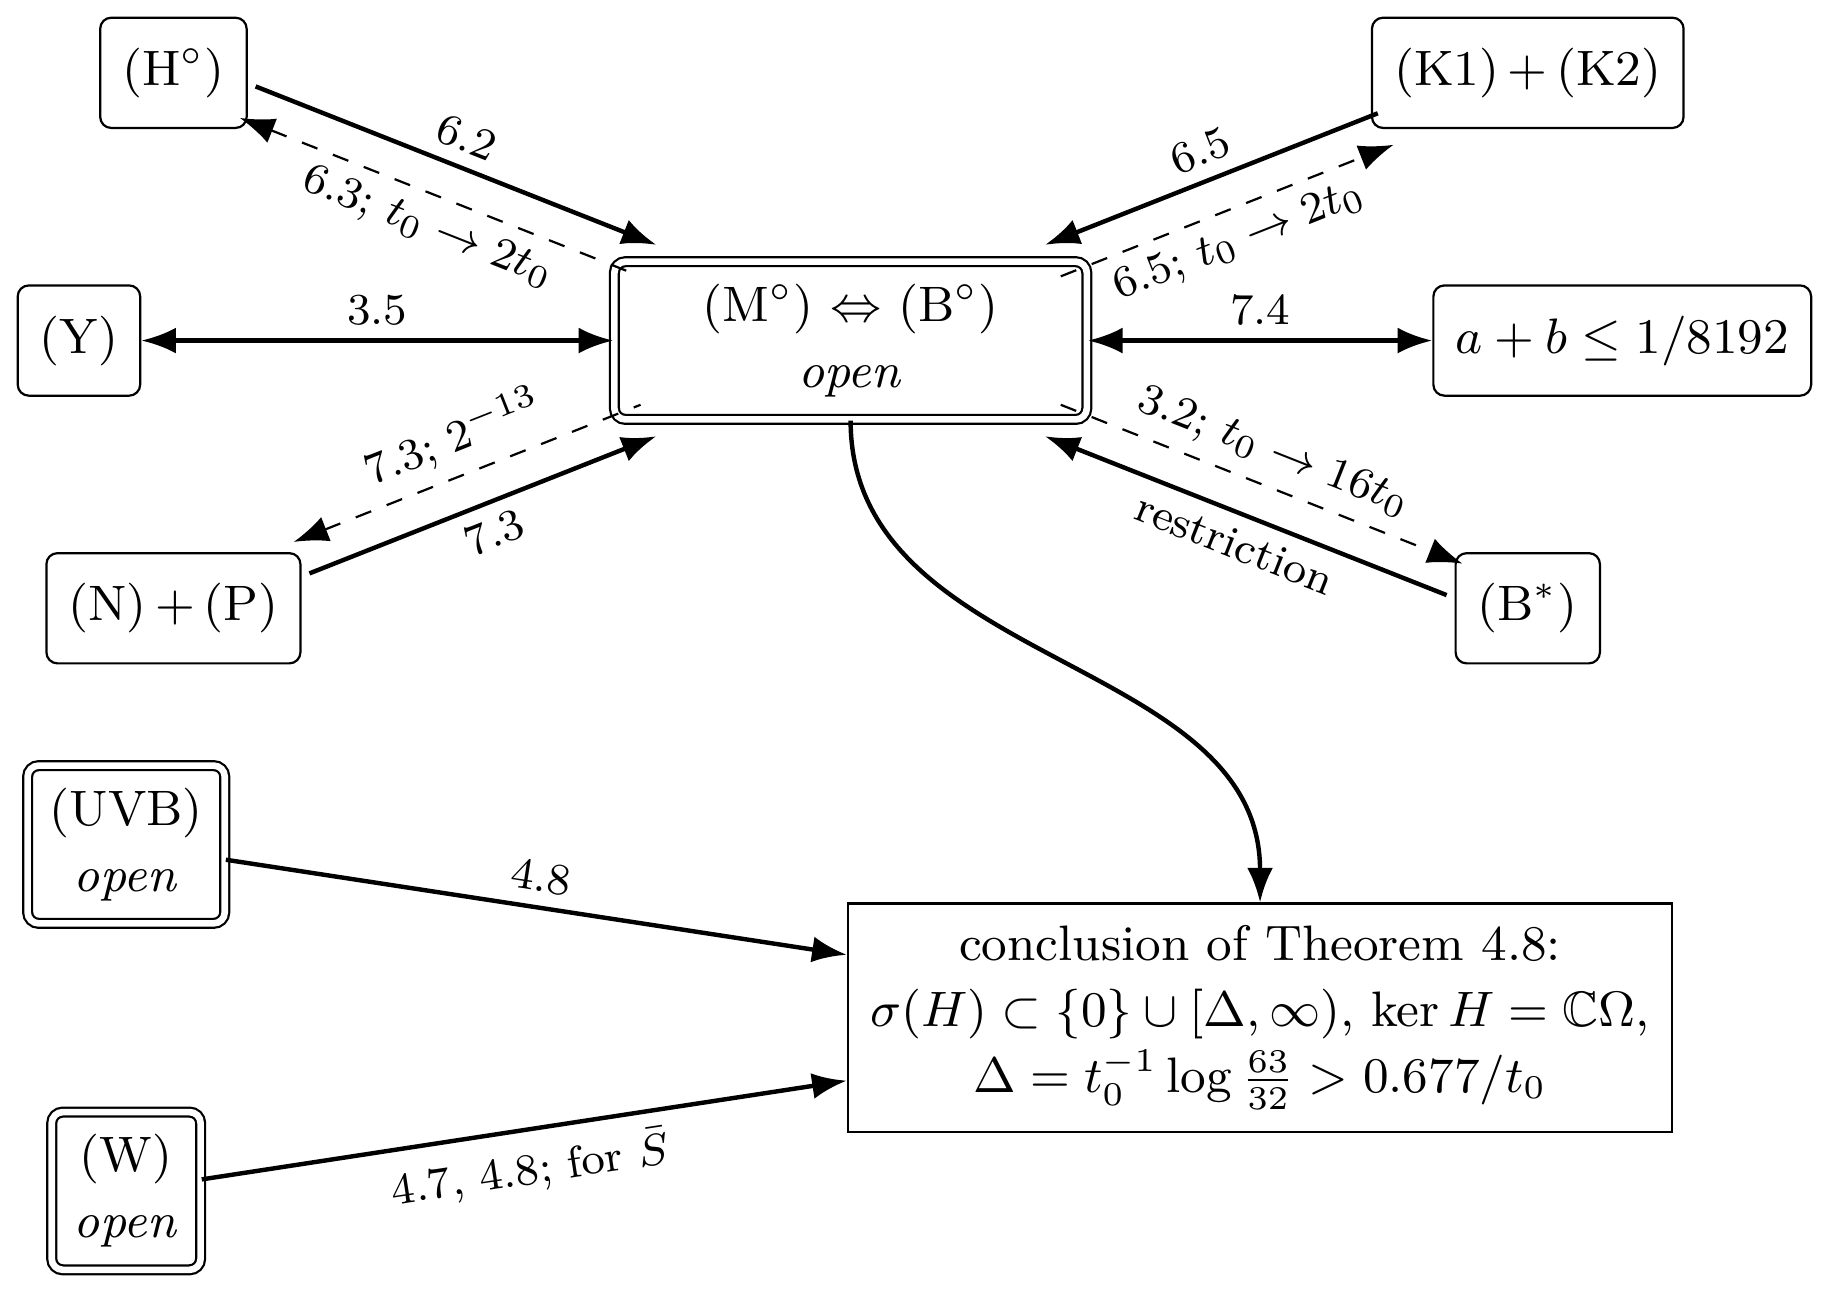
\includegraphics[width=329.2bp]{figures/fig01.png}
\caption{Reduction graph. Solid arrows are implications and double-headed arrows equivalences proved in this paper, labelled by the result that proves them; dashed arrows are converses, labelled by their loss ($\tzero$ multiplied by $2$ or $16$, or tolerance $2^{-13}$ in \hypN{} and \hypP). Arrows at the central node refer to \Bcirc{} at the same $\Tzero$, except the equivalence with \hypY{}, $\lim_{t\to\infty}y(t)=0$, which concerns the whole family; $a$, $b$ are as in \cref{thm:projected-split}. The equivalence $\Mcirc\Leftrightarrow\Bcirc$ holds along the family (\cref{thm:zero-one}); at a single $\Tzero$ only $\Mcirc\Rightarrow\Bcirc$ holds (\cref{lem:purity-conversion}). Every hypothesis node is unproved along the continuum tuning; the double frames mark the hypotheses of \cref{thm:main}. The conclusion at the bottom is conditional on \Mcirc{} and on \UVB, or on \hypW{} for the limit functional $\bar S$ of \hypW{} (\cref{prop:W-implies-UVB}).}
\label{fig:reduction}
\end{figure}

\Cref{fig:reduction} shows how \Mcirc{} is tied to the other forms of the open hypothesis proved in \cref{sec:ascent,sec:criteria,sec:centre}, and how it enters the continuum conclusion.

\subsection{The results in order}
\Cref{sec:psts} sets up positive symmetric torus systems with the exchange identity and the elongation inequality (\cref{lem:exchange,lem:elongation}). \Cref{sec:ascent} proves parts (i) and (ii) of Theorem~A, a variant with a gap on dyadic cubes (\cref{thm:dyadic-gap}), the zero--one law and the upward closure of the seed (\cref{thm:upward-closed}). \Cref{sec:continuum} proves part (iii); it also shows that under \hypW{} a nontrivial limit needs divergent normalisation of the insertions (\cref{thm:bounded-tokens}), and derives \UVB{} for the plaquette-energy insertion from an analyticity hypothesis \San{} that is not proved here (\cref{thm:San-UVB}).

\Cref{sec:constructed} applies part (iii) to the Wilson family of \cite{openaiym}: its ordered limit satisfies the convergence clause over its own lattice spacings (\cref{prop:index-sets,lem:oai-family}), so \Mcirc{} along its tuning, on which $\betaW$ grows like $\log(1/\aN)$, gives a gap of at least $\Delta$ for the unselected limit (\cref{thm:constructed-gap}), and an averaging argument over the phases transfers it to every phase (\cref{thm:constructed-phases}).

\Cref{sec:criteria} gives the hypercube form \Hcirc, which has no transfer matrix in its hypothesis, and the Casimir form \Kone+\Ktwo{} of the datum (\cref{thm:hypercube,thm:casimir-criterion}). \Cref{sec:centre} splits the datum along a finite subgroup of the centre into a centre-neutral part \hypN{} and an electric-flux part \hypP{} (\cref{thm:residue-split,thm:projected-split}), bounds the Polyakov-loop correlator under \Mcirc{} (\cref{prop:polyakov-bound}), and derives \hypP{} conditionally from a Hamiltonian area law with a count of flux states (\cref{thm:flux-count}); along the tuning it shows that \Mcirc{} is equivalent to a uniform gap and a bounded free energy in the centre-neutral sector together with a decay rate of 't~Hooft's vortex weight bounded below in physical units (\cref{thm:sector-criterion}), and that either rate may be replaced by a thermodynamic quantity tending to $0$ (\cref{thm:crossed-criteria}); each gap is then the exponential decay rate of the corresponding free energy, and the thresholds reduce to the critical value of the zero--one law (\cref{thm:decay-rates,cor:sharp-crossed}). \Cref{sec:ranges} proves the datum for $\tanh\betaW<1/18$ for every compact group, for $\betaW<2/9$ for $\SU(2)$, for $\betaW<N_c^2/48$ for $\SU(N_c)$, and in two dimensions (\cref{thm:strong-coupling,cor:certified-triples,thm:large-N,thm:two-dim}); these are strong-coupling statements and do not touch the continuum tuning.

\Cref{sec:necessary} proves necessary conditions on any proof: the gap of a fixed torus closes as the coupling grows, so the base scale must grow (\cref{thm:fixed-torus-gap,cor:base-scale}); the purity defect stays bounded away from $0$ on every fixed torus (\cref{thm:fixed-window,prop:flux-saturation,prop:flux-saturation-N}); the datum forces a spectral gap on the cube (\cref{prop:spectral-conditions}), cannot hold through a free-gluon count (\cref{prop:no-stefan-boltzmann,thm:free-gluon,thm:pair}), cannot hold for $\SU(N_c)$ and $\SU(N_c)/\Z_{N_c}$ at the same coupling (\cref{thm:exclusivity}), forces blocked fields to be disordered at the scale of the box (\cref{thm:box-disorder}), and requires a vortex rate that fails once the coupling grows like $N^{3+\delta}$ and fails for the heat-kernel $\U(1)$ theory at a logarithmic coupling (\cref{cor:fast-vortex,prop:abelian-vortex}); for $C=\{\pm1\}$ and a vanishing neutral free energy, the datum is equivalent to the vanishing of the averaged overlap defect of two slices, one of them flipped by the centre, at every ratio above $\frac12$ of their time separation to half the side of the box (\cref{thm:averaged-overlap,thm:overlap-criteria}). \Cref{sec:obstructions} proves obstructions: a decoupled gapped sector destroys \Mcirc{} while preserving reflection positivity and every link expectation (\cref{thm:hidden-sector}); data independent of $\beta$ cannot suffice (\cref{cor:beta-independent}); abelian theories violate the datum (\cref{thm:abelian}); Griffiths--Ginibre positivity fails for $\SU(2)$ (\cref{thm:pseudoreality}); finitely many finite-rank certificates do not suffice (\cref{thm:finite-rank-obstruction}); and stability, lattice reflection positivity and hypercubic invariance imply neither $O(4)$ invariance nor clustering (\cref{thm:non-implication}). \Cref{sec:identities} proves three exact identities (\cref{prop:thermal-response,prop:winding,thm:heat-kernel}), \cref{sec:ms} collects the thermal-purity results, including the stability of certified data under approximation (\cref{ms:prop:intervals}), an ascent lemma with errors (\cref{ms:lem:noisy-ascent}) and a gapless generalized free field with the ultraviolet trace coefficient of the free gluon (\cref{ms:prop:GFF}), with proofs in \cref{app:ms-proofs}, and \cref{sec:wall} lists the equivalent forms of the open datum and the requirements on any proof (\cref{tab:wall,fig:wall}). The constants and finite computations are certified in \cref{app:certificates}, and \cref{app:verification} lists their machine checks in Lean~4 \cite{demoura2021,mathlib2020} and Julia \cite{bezanson2017}.

\subsection{Relation to the first paper}
Theorem~A of \cite{bhattacharjee2026first} proves the lattice mass gap at strong coupling for every compact simple group with explicit rates, and Theorem~F of \cite{bhattacharjee2026first} shows that \hypW{} together with the hypothesis \Bstar, the bound $\log\Zs{s}{T_0}\le\gamma\Vol{s}$ with $2\gamma(96T_0)^3\le1/20$ for all spatial tori with sides in $[2T_0,48T_0)$, gives a continuum mass gap $\Delta\ge0.172/\tzero$ and a unique vacuum. Theorem~A above needs the datum on one torus pair: restricted to the cube, \Bstar{} asks $\XT{\cube{T_0}}{T_0}\le1/4\,423\,680$, while \Bcirc{} asks $\XT{\cube{T_0}}{T_0}\le\xconstinl$ and nothing on other shapes. The hypothesis \Bstar{} at $\Tzero$ implies \Bcirc{} at $\Tzero$, and \Bcirc{} at $\Tzero$ implies \Bstar{} at $16\Tzero$ (\cref{thm:ascent,cor:window-datum}). Theorem~A above replaces \hypW{} by \UVB{} and the constant $0.172$ by $0.677$. Results of \cite{bhattacharjee2026first} used in proofs are either restated with proofs in \cref{app:first-paper} or cited by exact number at the point of use. The cited results include the identification with the phase form of \hypW{} (Theorem~F(iii) of \cite{bhattacharjee2026first}, \cref{cor:phase-form}), which no other result of this paper uses, and the sharp Kantorovich modulus $1/4$ of the von Mises--Fisher family on $\SU(2)$ (Theorem~A1 of \cite{bhattacharjee2026first}), which gives the $\SU(2)$ constant in \cref{thm:strong-coupling}. Published theorems of other authors are quoted at their point of use with their hypotheses checked.

\subsection{Related work}
At strong coupling Osterwalder and Seiler proved confinement and a mass gap by convergent expansions \cite{osterwalder1978}; Seiler's monograph \cite{seiler1982} sets out this framework, and Cao, Nissim and Sheffield \cite{cao2025expanded} enlarge the range of couplings with an area law. In a finite volume at weak coupling, Ba{\l}aban's renormalisation group for four-dimensional lattice gauge theories \cite{balaban1987,balaban1988a,balaban1988b,balaban1989a,balaban1989b} controls the effective actions under the condition that all effective coupling constants stay small; its published output is a bound on the effective densities. Brydges \cite{brydges2009} gives lectures on the renormalisation group, Dimock \cite{dimock2013} an expository account of the method for the scalar $\varphi^4$ model in three dimensions, and Magnen, Rivasseau and S\'en\'eor \cite{magnen1993} treat four-dimensional $\SU(2)$ theory with an infrared cutoff in a regularised axial gauge. None of these results is used in a proof below. The centre grading of \cref{sec:centre} is 't~Hooft's decomposition into electric and magnetic flux sectors through twisted boundary conditions \cite{thooft1979}; Tomboulis and Yaffe \cite{tomboulis1985} bounded Wilson loops by vortex free energies, Kanazawa \cite{kanazawa2009} extended their inequality to $\SU(N)$ lattice gauge theories, and Borgs and Seiler \cite{borgs1983} studied lattice Yang--Mills theory at nonzero temperature in connection with confinement. L\"uscher \cite{luscher1983} and van Baal and Koller \cite{koller1987} computed the low-lying spectrum of Yang--Mills theory on small tori. On the probabilistic side, Chatterjee \cite{chatterjee2021} proved that unbroken centre symmetry implies confinement, and Adhikari and Cao \cite{adhikari2025} proved exponential decay of correlations for finite gauge groups at weak coupling; Chatterjee \cite{chatterjee2019} surveys the problem for probabilists, and \cite{chatterjee2016} computes the leading term of the lattice free energy as the lattice spacing tends to zero. These are statements at a fixed lattice spacing; the datum \Mcirc{} concerns the coupling and the scale of the continuum tuning.

For every compact simple group, the Lean~4 development \cite{openaiym} constructs a Wilson family whose ordered continuum limit is a mixture of phases, with a selected phase that reconstructs a nontrivial Wightman theory with a unique vacuum; the construction was assessed in \cite{ymgroup2026}, the mass gap and the uniqueness of the infinite-volume limit are outside its statement, and \cref{sec:constructed} connects it with the datum. In two dimensions, Piazza and Shen \cite{piazza2026} proved a log-Sobolev inequality for the $\SU(N)$ Wilson measure at every fixed inverse coupling with a constant uniform in the volume, and Bringmann, Cao, Hairer and Zhao \cite{bringmann2026} constructed the two-dimensional non-abelian Yang--Mills--Higgs measure by stochastic quantisation; \cref{thm:two-dim} below concerns the same dimension by a different route. In four dimensions, Mihajlovic \cite{mihajlovic2026} gives finite-volume spectral bounds for $\SU(2)$ and criteria for transferring them to a continuum limit, and records that a four-dimensional construction with a positive spectral bound is not obtained there. The weak-coupling side of the present paper, the tuning $\beta\to\infty$ along which the datum must be checked, is not reached by any of these results.
\section{Positive symmetric torus systems}\label{sec:psts}

The $\beta$-free results of \cref{sec:ascent,sec:criteria}, and the reductions in the later sections, are statements about one abstract class of partition functions on four-dimensional tori. This section defines the class, shows that it contains Wilson lattice gauge theory for every compact gauge group and every $\beta\ge0$, and every theory with a positive-definite class weight, and proves the elementary facts about the class that the later sections use.

\subsection{Tori, systems and the datum}

For $n=(n_1,n_2,n_3,n_4)\in\Z^4$ with all $n_\mu\ge3$ let $\Lambda(n)=\prod_{\mu=1}^4\Z/n_\mu\Z$ and $|n|=n_1n_2n_3n_4$. A \emph{spatial torus} is a triple $s=(s_1,s_2,s_3)$ of integers $s_j\ge3$, with volume $\Vol{s}=s_1s_2s_3$. We write $(s,M)$ for $(s_1,s_2,s_3,M)$ and call its last entry time; $L^3$ stands for $(L,L,L)$ and $L^4$ for $(L^3,L)$, so that $\cube{T}$ is the spatial cube of side $2T$.

A \emph{positive symmetric torus system} (\PSTS) is a function $n\mapsto Z(n)$ on $\{n\in\Z^4:n_\mu\ge3\}$ with the following two properties.
\begin{enumerate}[label=(P\arabic*),leftmargin=3em]
\item $Z(n)\ge1$, and $Z(\pi n)=Z(n)$ for every permutation $\pi$ of the four entries of $n$.
\item For every spatial torus $s$ there is a nonzero self-adjoint Hilbert--Schmidt operator $\TT_s\ge0$ on a separable Hilbert space $\Kspace_s$ such that $\Zpart{s}{M}=\Tr\TT_s^M$ for all $M\ge3$.
\end{enumerate}
The system is \emph{simple} if the largest eigenvalue of every $\TT_s$ is simple. Simplicity is not part of the definition: \cref{lem:simplicity-not-needed} shows that the argument of \cref{sec:ascent} does not use it and that it follows from the datum on large cubes.

Let $\lzero(s)=\norm{\TT_s}>0$; it is an eigenvalue of finite multiplicity, and $E_0(s)=-\log\lzero(s)$. The operator $R_s=\TT_s/\lzero(s)$ has eigenvalues $1=r_0(s)\ge r_1(s)\ge r_2(s)\ge\dots\ge0$, listed with multiplicity, and $\sum_ir_i(s)^2<\infty$. Thus $r_1(s)=1$ exactly when $\lzero(s)$ is degenerate, and $-\log r_1(s)$ is the spectral gap of $\TT_s$ in lattice units. For $T\ge2$ the operator $R_s^T$ is trace class, and we set
\begin{equation}\label{eq:normalised}
\Zs{s}{T}=\Tr R_s^T=\sum_{i\ge0}r_i(s)^T,\qquad \XT{s}{T}=\log\Zs{s}{T},\qquad \Dexc{s}{T}=\Zs{s}{T}-1 .
\end{equation}
For $T\ge3$ one has $\Zs{s}{T}=\Zpart{s}{T}/\lzero(s)^T$, and the purity defect is
\begin{equation}\label{eq:psi-def}
\psiT{s}{T}=2\log\Zpart{s}{T}-\log\Zpart{s}{2T}=2\XT{s}{T}-\XT{s}{2T}.
\end{equation}
Multiplying $Z(n)$ by $e^{a|n|}$, $a\in\R$, replaces $\TT_s$ by $e^{a\Vol{s}}\TT_s$ and changes neither $R_s$ nor any of the quantities in \eqref{eq:normalised} and \eqref{eq:psi-def}.

\smallskip
\noindent\emph{The datum.} Let $\Tzero\ge3$ be an integer. The system satisfies \Mcirc{} at $\Tzero$ if
\begin{equation}\label{eq:datum-M}
\psiT{\cube{T_0}}{T_0}\le\dconst,\qquad\text{equivalently}\qquad \Zpart{\cube{T_0}}{T_0}^2\le e^{\dconstinl}\,Z\bigl((2T_0)^4\bigr),
\end{equation}
and it satisfies \Bcirc{} at $\Tzero$ if
\begin{equation}\label{eq:datum-B}
\XT{\cube{T_0}}{T_0}\le\xconst .
\end{equation}
By \cref{lem:purity-conversion}, \Mcirc{} at $T_0$ implies \Bcirc{} at $T_0$, which in turn implies $\psiT{\cube{T_0}}{T_0}\le1/4096$. For the continuum family of \cref{def:continuum-family} we say that \Mcirc{} holds \emph{along the tuning} with $\tzero>0$ if for every sufficiently large $p$ there is $N_0(p)$ such that for every $N\ge N_0(p)$ of the family the Wilson system at coupling $\betaNp$ satisfies \Mcirc{} at some integer $\Tzero$ with $3\le\Tzero\le N\tzero$; the same convention is used for \Bcirc{}. The ranges in which it is proved lie at strong coupling or in two dimensions (\cref{sec:ranges}).

\subsection{Wilson theory and positive-definite class weights}

Let $G\subset\U(N_c)$ be a closed subgroup, hence a compact Lie group, with normalised Haar measure $\dd g$.\footnote{We write $N_c$ for the size of the matrices because $N=1/\aN$ denotes the inverse lattice spacing of the continuum family in \cref{def:continuum-family}.} A configuration on $\Lambda(n)$ assigns $U_{(x,\mu)}\in G$ to the link from $x$ to $x+e_\mu$. The plaquette at $x$ in the $(\mu,\nu)$-plane carries $Q_p=U_{(x,\mu)}U_{(x+e_\mu,\nu)}U_{(x+e_\nu,\mu)}^*U_{(x,\nu)}^*$, and $\ReTr Q_p$ depends neither on the base point nor on the orientation of $p$. For $\beta\ge0$ the Wilson weight \cite{wilson1974} and partition function are
\begin{equation}\label{eq:wilson-weight}
W_n(U)=\exp\Bigl(N_c\beta\sum_p\ReTr Q_p\Bigr),\qquad Z(n)=\int W_n(U)\prod_{(x,\mu)}\dd U_{(x,\mu)},
\end{equation}
where $p$ runs over the $6|n|$ unoriented plaquettes; $\betaW=N_c^2\beta$ is the usual Wilson coupling, and $\betaW=4\beta$ for $\SU(2)$.

Write $n=(s,M)$, let $\Lambda_s=\prod_{j=1}^3\Z/s_j\Z$, and let $E_s$ be the set of the $3\Vol{s}$ links of $\Lambda_s$. At time $t\in\Z/M\Z$ the spatial links form $Q^{(t)}\in G^{E_s}$, and the temporal links from $t$ to $t+1$ form $U^{(t)}=(U_x)_{x\in\Lambda_s}\in G^{\Lambda_s}$. Let $S_s(Q)$ be the sum of $\ReTr Q_p$ over the $3\Vol{s}$ plaquettes of $\Lambda_s$ and
\[
S_0(Q,U,Q')=\sum_{x\in\Lambda_s}\sum_{i=1}^3\ReTr\bigl(Q_{(x,i)}U_{x+e_i}Q'^{*}_{(x,i)}U_x^*\bigr),
\]
so that $\sum_p\ReTr Q_p=\sum_t\bigl[S_s(Q^{(t)})+S_0(Q^{(t)},U^{(t)},Q^{(t+1)})\bigr]$. On $\Kspace=L^2(G^{E_s})$ let $\TT_s$ be the integral operator with kernel
\begin{equation}\label{eq:transfer-kernel}
\TT_s(Q,Q')=\int_{G^{\Lambda_s}}\exp\Bigl(N_c\beta\bigl[\tfrac12S_s(Q)+\tfrac12S_s(Q')+S_0(Q,U,Q')\bigr]\Bigr)\prod_{x\in\Lambda_s}\dd U_x .
\end{equation}
Gauge transformations $U\in G^{\Lambda_s}$ act on $G^{E_s}$ by $(U\cdot Q)_{(x,i)}=U_xQ_{(x,i)}U_{x+e_i}^*$ and preserve Haar measure; $\Pi=\int R_U\dd U$, with $(R_Uf)(Q)=f(U^{-1}\cdot Q)$, is the orthogonal projection onto gauge-invariant functions. Let $D$ be multiplication by $e^{N_c\beta S_s/2}$ (this operator is unrelated to the excess $\Dexc{s}{T}$ of \eqref{eq:normalised}, which always carries its two arguments), and let $K$ be the operator with kernel $K(Q,Q')=\exp\bigl(N_c\beta\sum_{e\in E_s}\ip{Q_e}{Q'_e}_{\R}\bigr)$, where $\ip{A}{B}_{\R}=\ReTr(AB^*)$. For $c$ in the centre of $G$ and $j\in\{1,2,3\}$ let $\zeta_j^c$ multiply $Q_{(x,j)}$ by $c$ for every $x$ with $x_j=0$, leaving the other links unchanged, and let $(z_j^cf)(Q)=f(\zeta_j^cQ)$.

\begin{lemma}[{(i)--(iii): \cite[Lemma~11(i),(ii),(vii)]{bhattacharjee2026first}, \cite{osterwalder1978,luscher1977,creutz1977}; (iv): centre symmetry \cite{thooft1979}}]\label{lem:transfer-matrix}
Let $G\subset\U(N_c)$ be closed, $\beta\ge0$, and $s$ a spatial torus.
\begin{enumerate}[label=(\roman*)]
\item The kernel \eqref{eq:transfer-kernel} is continuous, strictly positive and symmetric. $\TT_s$ is self-adjoint and Hilbert--Schmidt, $\TT_s=D\Pi K\Pi D$ with $K\ge0$, and hence $\TT_s\ge0$.
\item $\lzero(s)=\norm{\TT_s}$ is a simple eigenvalue whose eigenvector $\Omegazero$ can be chosen continuous and strictly positive. Every eigenvector with a nonzero eigenvalue is gauge invariant.
\item $\Zpart{s}{M}=\Tr\TT_s^M$ for $M\ge3$, $Z(n)\ge1$, and $Z$ is symmetric in $n_1,\dots,n_4$. Thus Wilson theory is a simple \PSTS{}.
\item For $c$ central and $j\le3$, $z_j^c$ is unitary and commutes with $\TT_s$ and with every $R_U$, and $z_j^c\Omegazero=\Omegazero$.
\end{enumerate}
\end{lemma}

\begin{proof}
(i) The integrand of \eqref{eq:transfer-kernel} is continuous and strictly positive on a compact space, so the kernel is continuous, strictly positive and bounded, and $\TT_s$ is Hilbert--Schmidt. From $\ReTr A=\ReTr A^*$ and cyclicity, $S_0(Q',U,Q)=S_0(Q,U^*,Q')$ with $U^*=(U_x^*)_x$; inversion preserves Haar measure, so the real kernel is symmetric and $\TT_s$ is self-adjoint. Next, $S_0(Q,U,Q')=\sum_e\ip{Q_e}{(U\cdot Q')_e}_{\R}$, so
\[
\TT_s(Q,Q')=e^{N_c\beta S_s(Q)/2}\Bigl[\int K(Q,U\cdot Q')\dd U\Bigr]e^{N_c\beta S_s(Q')/2},
\]
and the substitution $Q''=U\cdot Q'$ identifies the bracket with the kernel of $K\Pi$. Since $\ip{U_xAU_y^*}{U_xBU_y^*}_{\R}=\ip{A}{B}_{\R}$, $K$ commutes with every $R_U$ and with $\Pi$, so $K\Pi=\Pi K\Pi$; $S_s$ is gauge invariant, so $D$ commutes with $\Pi$. Hence $\TT_s=D\Pi K\Pi D=(\Pi D)^*K(\Pi D)$. To see $K\ge0$, identify $M_{N_c}(\C)$ with $\R^{2N_c^2}$ through the real and imaginary parts of the entries; then $\ip{A}{B}_{\R}$ is the Euclidean inner product. Let $\Phi(Q)\in\R^d$, $d=2N_c^2|E_s|$, collect the coordinates of all $Q_e$, and $\kappa=N_c\beta$. Then $K(Q,Q')=\sum_{k\ge0}\frac{\kappa^k}{k!}\ip{\Phi(Q)^{\otimes k}}{\Phi(Q')^{\otimes k}}$, uniformly on $G^{E_s}\times G^{E_s}$, and for $f\in\Kspace$
\[
\ip{f}{Kf}=\sum_{k\ge0}\frac{\kappa^k}{k!}\,\Bigl\lVert\int f(Q)\,\Phi(Q)^{\otimes k}\dd Q\Bigr\rVert^2\ge0,
\]
the norm being the Euclidean norm on $(\R^d)^{\otimes k}\otimes\C$. So $\ip{f}{\TT_sf}=\ip{\Pi Df}{K\Pi Df}\ge0$, and $\TT_s\ne0$ because its kernel is positive.

(ii) An eigenvector $h$ with eigenvalue $\lambda\ne0$ equals $\lambda^{-1}\TT_sh$, so it is continuous, and it lies in the range of $\Pi$ because $\TT_s=\Pi(DKD)\Pi$. Since $\TT_s\ge0$ is compact, $\lzero=\norm{\TT_s}$ is the maximum of $\ip{h}{\TT_sh}$ over unit vectors, and a unit vector $g$ attains it only if $\norm{(\lzero-\TT_s)^{1/2}g}=0$, that is, only if $\TT_sg=\lzero g$. Let $h$ be a unit eigenvector for $\lzero$. Then $\ip{\abs{h}}{\TT_s\abs{h}}\ge\abs{\ip{h}{\TT_sh}}=\lzero$, so $\TT_s\abs{h}=\lzero\abs{h}$, and for every $Q$
\[
\lzero\abs{h(Q)}=\int\TT_s(Q,Q')\abs{h(Q')}\dd Q'>0,\qquad \lzero\abs{h(Q)}=\Bigl\lvert\int\TT_s(Q,Q')h(Q')\dd Q'\Bigr\rvert .
\]
Equality in the triangle inequality, with a continuous strictly positive weight and a measure of full support, forces $h=e^{i\theta}\abs{h}$ for a constant $\theta$. So every eigenvector for $\lzero$ is a constant multiple of a strictly positive continuous function. Two such functions are never orthogonal, hence $\lzero$ is simple; put $\Omegazero=\abs{h}$. The argument is that of Jentzsch \cite{jentzsch1912}.

(iii) Integrating first over the temporal links, each of which occurs in one factor $S_0(Q^{(t)},U^{(t)},Q^{(t+1)})$, and splitting each $S_s(Q^{(t)})$ into two halves gives
\[
\Zpart{s}{M}=\int\prod_{t\in\Z/M\Z}\TT_s(Q^{(t)},Q^{(t+1)})\prod_t\dd Q^{(t)} .
\]
The kernel of $\TT_s^{M-1}$ is the iterated integral, and $\Tr(AB)=\iint A(Q,Q')B(Q',Q)\dd Q\dd Q'$ for Hilbert--Schmidt operators $A,B$; hence $\Zpart{s}{M}=\Tr\TT_s^M$. A permutation of the axes maps links to links and plaquettes to plaquettes, possibly reversing orientation, which leaves $\ReTr Q_p$ unchanged, and it preserves the product Haar measure; so $Z(\pi n)=Z(n)$. By Jensen's inequality $Z(n)\ge\exp\bigl(N_c\beta\sum_p\int\ReTr Q_p\prod\dd U\bigr)$. The four links of $p$ are distinct because $n_\mu\ge3$, and for fixed values of the other three, $Q_p$ is $U_{(x,\mu)}$ times a fixed element of $G$; so $Q_p$ is Haar distributed and $\int\ReTr Q_p=\ReTr P_G$, where $P_G=\int_Gg\dd g$ is the orthogonal projection of $\C^{N_c}$ onto the $G$-invariant vectors. Thus $\int\ReTr Q_p=\rank P_G\ge0$ and $Z(n)\ge1$.

(iv) $\zeta_j^c$ preserves Haar measure, so $z_j^c$ is unitary. A spatial plaquette in a $(j,k)$-plane contains the two $j$-links $(x,j)$ and $(x+e_k,j)$, which have the same $j$-coordinate; either both or neither are multiplied by $c$, and in the first case $Q_p$ becomes
\[
cU_{(x,j)}U_{(x+e_j,k)}U^*_{(x+e_k,j)}c^*U^*_{(x,k)}=Q_p,
\]
since $c$ is central and unitary. The plaquettes in the plane of the two other spatial directions contain no $j$-link. In $S_0$ the terms with $i=j$ and $x_j=0$ become
\[
\ReTr\bigl(cQ_{(x,j)}U_{x+e_j}Q'^*_{(x,j)}c^*U_x^*\bigr)=\ReTr\bigl(Q_{(x,j)}U_{x+e_j}Q'^*_{(x,j)}U_x^*\bigr),
\]
equal to the old terms, and all other terms are unchanged. Hence $\TT_s(\zeta_j^cQ,\zeta_j^cQ')=\TT_s(Q,Q')$, and the measure-preserving substitution $Q'\mapsto\zeta_j^cQ'$ gives $z_j^c\TT_s=\TT_sz_j^c$. As $\zeta_j^c(U\cdot Q)=U\cdot\zeta_j^cQ$, $z_j^c$ commutes with every $R_U$. Finally $z_j^c\Omegazero$ is a strictly positive eigenvector for $\lzero$ with the norm of $\Omegazero$, so $z_j^c\Omegazero=\Omegazero$ by (ii).
\end{proof}

The same holds for every plaquette weight of positive type. Let $\Fclass(G)$ be the set of continuous class functions $f\colon G\to(0,\infty)$ with $f_\lambda=\int_Gf(g)\overline{\chi_\lambda(g)}\dd g\ge0$ for every irreducible unitary representation $\lambda$ of $G$, of character $\chi_\lambda$ and dimension $d_\lambda$; these are the positive-definite class weights. On $L^2(G)$ let $(C_f\varphi)(g)=\int_Gf(gh^{-1})\varphi(h)\dd h$.

\begin{proposition}\label{prop:class-weight-psts}
Let $f\in\Fclass(G)$. Then $f(g^{-1})=f(g)$, and
\[
Z_f(n)=\bigl(\min\nolimits_Gf\bigr)^{-6|n|}\int\prod_pf(Q_p)\prod_{(x,\mu)}\dd U_{(x,\mu)}
\]
is a simple \PSTS{}; the prefactor does not change its normalised quantities. Statements (i)--(iv) of \cref{lem:transfer-matrix} hold with $\exp(N_c\beta\ReTr\,\cdot\,)$ replaced by $f$, $D$ by multiplication by $\prod_pf(Q_p)^{1/2}$ over the plaquettes of $\Lambda_s$, and $K$ by $\bigotimes_{e\in E_s}C_f\ge0$. The class $\Fclass(G)$ contains the Wilson weight $g\mapsto\exp(N_c\beta\ReTr g)$ for every $\beta\ge0$, and for $G=\U(1)$ it contains the heat-kernel weight $p_t(\varphi)=\sum_{k\in\Z}e^{-tk^2/2}e^{ik\varphi}$, $t>0$, which is a constant multiple of the Villain weight $\sum_{m\in\Z}e^{-(\varphi-2\pi m)^2/(2t)}$.
\end{proposition}

\begin{proof}
The characters form an orthonormal basis of the square-integrable class functions, so $f=\sum_\lambda f_\lambda\chi_\lambda$ in $L^2(G)$, and since $f$ and the $f_\lambda$ are real, $f(g)=\overline{f(g)}=\sum_\lambda f_\lambda\chi_\lambda(g^{-1})=f(g^{-1})$, first in $L^2$ and then pointwise by continuity. As $f$ is also a class function, $f(Q_p)$ depends neither on the base point nor on the orientation of $p$. Replacing $f$ by $f/\min f$ multiplies the integral by $(\min f)^{-6|n|}$, which does not change the normalised quantities, and makes the integrand at least $1$; so $Z_f\ge1$, and we may assume $f\ge1$.

The proof of \cref{lem:transfer-matrix} applies once two facts are checked (cf.\ \cite[proof of Proposition~A5]{bhattacharjee2026first}, where the transfer matrix of a general class-function weight is written in the same form). First, the temporal factor is $f(Q_eU_{x+e_i}Q'^*_eU_x^*)=f\bigl(Q_e(U\cdot Q')_e^*\bigr)$, so the transfer kernel is $D_f(Q)\bigl[\int K_f(Q,U\cdot Q')\dd U\bigr]D_f(Q')$ with $D_f=\prod_pf(Q_p)^{1/2}$ and $K_f(Q,Q')=\prod_ef(Q_eQ'^*_e)$, the kernel of $\bigotimes_eC_f$. Because $f$ is a class function, $K_f$ is invariant under simultaneous gauge transformations and under $\zeta_j^c$, and because $f(g^{-1})=f(g)$ it is symmetric. Second, $C_f\ge0$: by the Peter--Weyl theorem the matrix coefficients $D^\lambda_{ab}$ of a complete set of irreducible representations form an orthogonal basis of $L^2(G)$, and Schur orthogonality gives $\chi_\mu*D^\lambda_{ab}=\delta_{\mu\lambda}D^\lambda_{ab}/d_\lambda$. Convolution with $D^\lambda_{ab}$ is continuous on $L^2(G)$, so $C_fD^\lambda_{ab}=f*D^\lambda_{ab}=(f_\lambda/d_\lambda)D^\lambda_{ab}$. Thus $C_f$ is diagonal in an orthogonal basis with eigenvalues $f_\lambda/d_\lambda\ge0$, so $C_f\ge0$ and $\bigotimes_eC_f\ge0$. Continuity and strict positivity of the kernel, the trace formula, the symmetry under permutations of the axes, simplicity and the statements on $z_j^c$ then follow as before.

For the Wilson weight let $\chi=\Tr$ be the character of the defining representation $V=\C^{N_c}$ of $G$ and $\kappa=N_c\beta\ge0$. Uniformly on $G$,
\[
e^{\kappa\ReTr g}=e^{\kappa(\chi(g)+\overline{\chi(g)})/2}=\sum_{a,b\ge0}\frac{(\kappa/2)^{a+b}}{a!\,b!}\,\chi(g)^a\,\overline{\chi(g)}^{\,b}.
\]
Each $\chi^a\bar\chi^b$ is the character of $V^{\otimes a}\otimes\bar V^{\otimes b}$, so its coefficient against $\chi_\lambda$ is the multiplicity of $\lambda$ in that representation, a nonnegative integer; hence every $f_\lambda\ge0$, and the weight is a continuous positive class function. For $\U(1)$ the characters are $e^{ik\varphi}$ and the coefficients of $p_t$ are $e^{-tk^2/2}>0$. Poisson summation gives $p_t(\varphi)=(2\pi/t)^{1/2}\sum_{m\in\Z}e^{-(\varphi-2\pi m)^2/(2t)}>0$, which is also the relation with the Villain weight.\footnote{For a general compact Lie group the heat-kernel weight has the coefficients $d_\lambda e^{-tc_\lambda/2}\ge0$, $c_\lambda$ the Casimir eigenvalue, so it belongs to $\Fclass(G)$ as soon as it is strictly positive. Only the case $\U(1)$ is used in this paper.}
\end{proof}

The following elementary bounds hold in every \PSTS{}.

\begin{lemma}[{\cite[Lemmas~15, 22 and 25]{bhattacharjee2026first}}]\label{lem:E1-E3}
Let $Z$ be a \PSTS{} and $s$ a spatial torus.
\begin{enumerate}[label=(E\arabic*),leftmargin=3em]
\item $\lzero(s)=\lim_{M\to\infty}\Zpart{s}{M}^{1/M}\ge1$, so $E_0(s)\le0$; $\lzero(s)$ and $\Zs{s}{M}$, $M\ge3$, are invariant under permutations of $s_1,s_2,s_3$.
\item $1\le\Zs{s}{M}\le\Zs{s}{2}<\infty$, and $M\mapsto\Zs{s}{M}$ is nonincreasing on $M\ge2$. For $M',M''\ge2$, $\Dexc{s}{M'+M''}\le\Dexc{s}{M'}\Dexc{s}{M''}$. If $r_1(s)\le e^{-\delta}$ with $\delta\ge0$, then $\Dexc{s}{M}\le e^{-\delta(M-M')}\Dexc{s}{M'}$ for $M\ge M'\ge2$.
\item For $T\ge3$ let $p_i=r_i(s)^T/\Zs{s}{T}$. Then $e^{-\psiT{s}{T}}=\sum_ip_i^2$, $p_0\ge p_i$ for all $i$, and
\begin{equation}\label{eq:X-psi}
\XT{s}{T}\le\psiT{s}{T}\le2\,\XT{s}{T}.
\end{equation}
The constants $1$ and $2$ cannot be improved.
\end{enumerate}
\end{lemma}

\begin{proof}
(E1) By (P2), $\Zpart{s}{M}=\sum_i\lambda_i^M$ over the eigenvalues $\lambda_i\ge0$ of $\TT_s$, with multiplicity. For $M\ge3$, $\lzero^M\le\Zpart{s}{M}\le\lzero^{M-2}\sum_i\lambda_i^2$, so $\Zpart{s}{M}^{1/M}\to\lzero(s)$, and $\lzero(s)\ge1$ because $Z\ge1$. By (P1), $\Zpart{s}{M}$ is invariant under permutations of $s$ at fixed $M$, hence so are $\lzero(s)$ and $\Zs{s}{M}=\Zpart{s}{M}/\lzero(s)^M$.

(E2) $\Zs{s}{M}=\sum_ir_i^M$ with $r_0=1$ and $0\le r_i\le1$ gives the first two claims. Next, $\Dexc{s}{M'+M''}=\sum_{i\ge1}r_i^{M'}r_i^{M''}\le\sum_{i\ge1}r_i^{M'}\sum_{k\ge1}r_k^{M''}$, the omitted cross terms being nonnegative. If $r_i\le e^{-\delta}$ for $i\ge1$, then $\Dexc{s}{M}=\sum_{i\ge1}r_i^{M'}r_i^{M-M'}\le e^{-\delta(M-M')}\Dexc{s}{M'}$.

(E3) By \eqref{eq:psi-def}, $e^{-\psiT{s}{T}}=\Zs{s}{2T}/\Zs{s}{T}^2=\sum_ip_i^2$, and $p_0=1/\Zs{s}{T}\ge p_i$ since $r_i\le1$. Hence $p_0^2\le\sum_ip_i^2\le p_0\sum_ip_i=p_0=e^{-\XT{s}{T}}$, which is \eqref{eq:X-psi}. For sharpness take $Z(n)=1+q\rho^{|n|}$ with an integer $q\ge1$ and $0<\rho<1$. It is a \PSTS{} with $\TT_s=\mathrm{diag}(1,\rho^{\Vol{s}},\dots,\rho^{\Vol{s}})$ on $\C^{1+q}$. With $a=\rho^{\Vol{s}T}$ one has $\XT{s}{T}=\log(1+qa)$ and $\psiT{s}{T}=2\log(1+qa)-\log(1+qa^2)$. As $\rho\uparrow1$ at fixed $q$ both tend to $\log(1+q)$, so $\psi/X\to1$; as $\rho\downarrow0$ with $q=1$, $\psi/X\to2$.
\end{proof}

\subsection{Exchange of directions and elongation}

Permutation symmetry lets one read the same torus with a spatial direction as time (\cref{fig:exchange}). For fixed transverse sides this turns the thermal trace of a long box into that of a short box, at the price of a free energy per unit length. The next lemma restates the cited results for an arbitrary \PSTS{}, with the same proof.

\begin{lemma}[{exchange of directions; \cite[Lemma~24(i) and Proposition~21(i)]{bhattacharjee2026first}}]\label{lem:exchange}
Let $Z$ be a \PSTS{}, fix integers $b,c\ge3$, and put $g(\ell)=\log\lzero(\ell,b,c)$ for $\ell\ge3$.
\begin{enumerate}[label=(\alph*)]
\item The limit $\bar e=\lim_{M\to\infty}g(M)/M$ exists and equals $\inf_{\ell\ge3}g(\ell)/\ell\in[0,g(3)/3]$. The function $\zeta(\ell)=g(\ell)-\ell\bar e$ satisfies $\zeta(\ell)=\lim_{M\to\infty}M^{-1}\log\Zs{(M,b,c)}{\ell}$, and it is nonnegative and nonincreasing on $\ell\ge3$.
\item For all integers $m,T\ge3$,
\begin{equation}\label{eq:exchange}
\log\Zs{(m,b,c)}{T}=m\,\zeta(T)-T\,\zeta(m)+\log\Zs{(T,b,c)}{m}.
\end{equation}
\item For every integer $T\ge3$, $\log\Zs{(2T,b,c)}{T}=\log\Zs{(T,b,c)}{2T}+T\delta_T$ with $\delta_T=2\zeta(T)-\zeta(2T)\in[\zeta(T),2\zeta(T)]$.
\end{enumerate}
By (E1) the same holds with the varying side in any of the three spatial positions.
\end{lemma}

\begin{proof}
By (P1), $Z((\ell,b,c),M)=Z((M,b,c),\ell)$ for $\ell,M\ge3$, that is,
\begin{equation}\label{eq:exchange-basic}
M\,g(\ell)+\log\Zs{(\ell,b,c)}{M}=\ell\,g(M)+\log\Zs{(M,b,c)}{\ell}.
\end{equation}
Divide by $\ell M$. Since $\log\Zs{(M,b,c)}{\ell}\ge0$ and $0\le\log\Zs{(\ell,b,c)}{M}\le\log\Zs{(\ell,b,c)}{2}<\infty$ by (E2), $g(M)/M\le g(\ell)/\ell+\log\Zs{(\ell,b,c)}{2}/(\ell M)$. Hence $\limsup_Mg(M)/M\le\inf_\ell g(\ell)/\ell\le\liminf_Mg(M)/M$, which gives $\bar e$ and the formula for it; $\bar e\ge0$ because $g\ge0$ by (E1). Dividing \eqref{eq:exchange-basic} by $M$ and letting $M\to\infty$ gives $g(\ell)=\ell\bar e+\lim_MM^{-1}\log\Zs{(M,b,c)}{\ell}$, the formula for $\zeta$. Then $\zeta\ge0$ since $\Zs{(M,b,c)}{\ell}\ge1$, and $\zeta$ is nonincreasing because $\ell\mapsto\Zs{(M,b,c)}{\ell}$ is, by (E2). Substituting $g(\ell)=\zeta(\ell)+\ell\bar e$ and $g(M)=\zeta(M)+M\bar e$ in \eqref{eq:exchange-basic}, the terms $\ell M\bar e$ cancel, and renaming $(M,\ell)$ as $(m,T)$ gives \eqref{eq:exchange}. Part (c) is \eqref{eq:exchange} at $m=2T$, and $\zeta(T)\le\delta_T\le2\zeta(T)$ follows from $0\le\zeta(2T)\le\zeta(T)$.
\end{proof}

\begin{figure}[htbp]
\centering
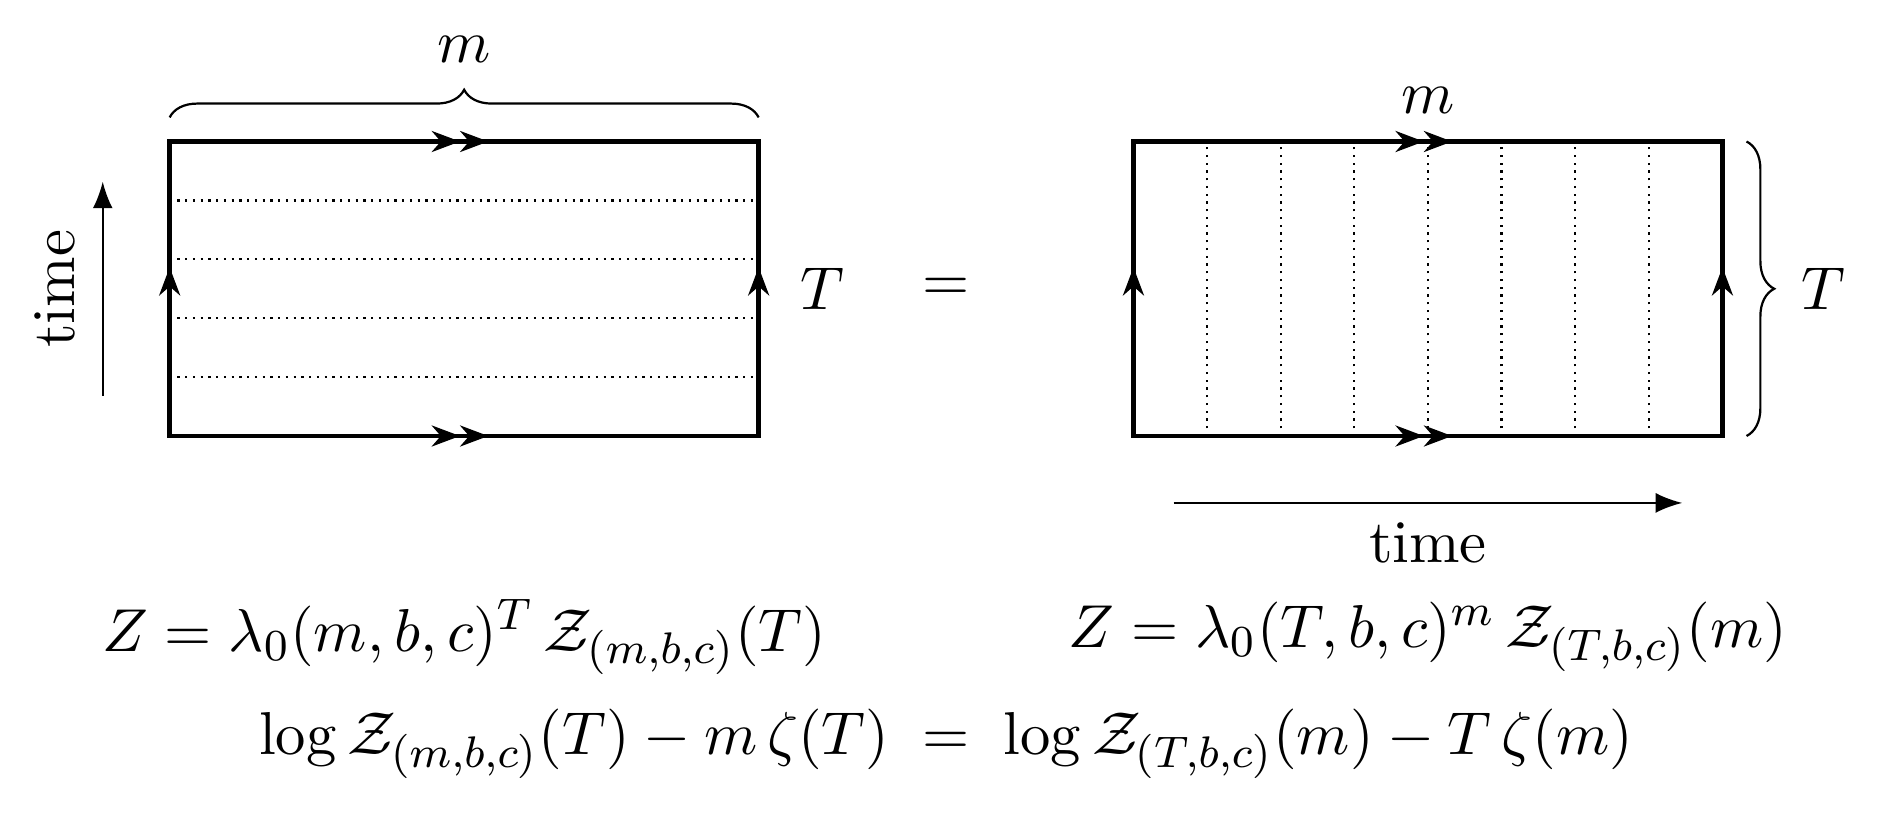
\includegraphics[width=338.7bp]{figures/fig02.png}
\caption{Exchange of directions (\cref{lem:exchange}): the torus $(m,b,c)\times T$ projected onto its first and fourth directions, with the directions of sides $b,c$ suppressed; arrows mark the periodic identifications. Left: time along the side $T$, the dotted slices are copies of the spatial torus $(m,b,c)$. Right: time along the side $m$, the slices are copies of $(T,b,c)$. Both readings compute the same $Z$; $\zeta(\ell)$ is the free energy per unit length of a long side when the other sides are $\ell,b,c$. \Cref{lem:elongation} uses that the right-hand trace does not increase with $m$.}
\label{fig:exchange}
\end{figure}

Since $\zeta(m)\ge0$ and the last term of \eqref{eq:exchange} does not increase with $m$, one side of a box can be made long at a cost proportional to its length.

\begin{lemma}[elongation]\label{lem:elongation}
Let $Z$ be a \PSTS{}, $b,c\ge3$, and let $m\ge m_0>T\ge3$ be integers. Put $L_0=\log\Zs{(m_0,b,c)}{T}$ and $Y_0=\log\Zs{(T,b,c)}{m_0}$. Then $0\le Y_0\le L_0$, $(m_0-T)\,\zeta(T)\le L_0-Y_0$, and
\begin{equation}\label{eq:elongation}
\log\Zs{(m,b,c)}{T}\le\frac{m}{m_0-T}\,(L_0-Y_0)+Y_0\le\frac{m}{m_0-T}\,\log\Zs{(m_0,b,c)}{T}.
\end{equation}
Consequently $\psiT{(m,b,c)}{T}\le\frac{2m}{m_0-T}\,\psiT{(m_0,b,c)}{T}$.
\end{lemma}

\begin{proof}
By \eqref{eq:exchange} at $m_0$, $L_0-Y_0=m_0\zeta(T)-T\zeta(m_0)\ge(m_0-T)\zeta(T)\ge0$, because $0\le\zeta(m_0)\le\zeta(T)$; and $Y_0\ge0$ by (E2). By \eqref{eq:exchange} at $m$, with $\zeta(m)\ge0$ and $\Zs{(T,b,c)}{m}\le\Zs{(T,b,c)}{m_0}$ from (E2),
\[
\log\Zs{(m,b,c)}{T}\le m\,\zeta(T)+Y_0\le\frac{m}{m_0-T}(L_0-Y_0)+Y_0 .
\]
As $m/(m_0-T)\ge1$, the right-hand side is at most $\frac{m}{m_0-T}L_0$. The last claim follows from \eqref{eq:X-psi}: $\psiT{(m,b,c)}{T}\le2\log\Zs{(m,b,c)}{T}\le\frac{2m}{m_0-T}L_0\le\frac{2m}{m_0-T}\psiT{(m_0,b,c)}{T}$.
\end{proof}

\subsection{Simplicity, purity conversion and decimation}

\begin{lemma}[simplicity is not needed]\label{lem:simplicity-not-needed}
\begin{enumerate}[label=(\roman*)]
\item The proofs of \cref{lem:E1-E3,lem:exchange,lem:elongation,lem:purity-conversion} and of \cref{thm:cube-control,thm:ascent,thm:dyadic-gap,thm:zero-one} do not use simplicity of $\lzero$; these results hold for every \PSTS{}, simple or not.
\item If a \PSTS{} satisfies \Bcirc{} at $T_0$, in particular if it satisfies \Mcirc{} at $T_0$, then $\lzero(t)$ is simple for every spatial torus $t$ whose sides all lie in one interval $[2T_i,4T_i)$, $T_i=2^iT_0$, $i\ge0$. This includes every cube $n^3$ with $n\ge2T_0$.
\end{enumerate}
\end{lemma}

\begin{proof}
(i) (E1) uses (P1), (P2) and $Z\ge1$, but not simplicity, (E2) only that $0\le r_i\le1$, (E3) and \cref{lem:purity-conversion} only that $p_0=1/\Zs{s}{T}\ge p_i$, whatever the multiplicity of $r_0=1$, and \cref{lem:exchange,lem:elongation} only (P1), (E1) and (E2). The proofs of \cref{thm:cube-control,thm:ascent,thm:dyadic-gap,thm:zero-one} use the system only through (P1), (E1)--(E3) and \cref{lem:exchange,lem:elongation,lem:purity-conversion}.

(ii) By (i), \cref{thm:ascent}(b) applies and gives $r_1(t)\le(32/63)^{1/T_0}<1=r_0(t)$, so $\lzero(t)$ is simple. Every integer $n\ge2T_0$ lies in $[2T_i,4T_i)$ for the $i\ge0$ with $2^{i+1}T_0\le n<2^{i+2}T_0$. Under \Mcirc{}, \cref{lem:purity-conversion} gives \Bcirc{}.
\end{proof}

For Wilson theory simplicity is part of \cref{lem:transfer-matrix}. Part (i) is what lets \cref{thm:ascent} apply to the twist-summed system $\bar Z$ of \cref{thm:exclusivity}, whose transfer matrices are direct sums and need not have a simple top eigenvalue.

\begin{lemma}[purity conversion]\label{lem:purity-conversion}
Let $Z$ be a \PSTS{}, $s$ a spatial torus, $T\ge3$ and $0<x\le1/8$. If $\psiT{s}{T}\le2x-3x^2$, then $\XT{s}{T}\le x$. In particular \Mcirc{} at $T_0$ implies \Bcirc{} at $T_0$, and \Bcirc{} at $T_0$ implies $\psiT{\cube{T_0}}{T_0}\le1/4096$.
\end{lemma}

\begin{proof}
Let $P=e^{-\psiT{s}{T}}=\sum_ip_i^2$ and $q=p_0=e^{-\XT{s}{T}}$, with $p_i$ as in (E3). Then $P\le q$ by (E3), and $P\le q^2+\bigl(\sum_{i\ge1}p_i\bigr)^2=h(q)$ with $h(y)=y^2+(1-y)^2$. Since $\psiT{s}{T}\le2x\le1/4$, $q\ge P\ge1-\psiT{s}{T}\ge3/4$. Suppose $\XT{s}{T}>x$, that is, $q<e^{-x}$. Now $e^{-x}\le q_U=1-x+\frac12x^2\le1$ and $h$ is strictly increasing on $[\frac12,1]$, so
\[
P\le h(q)<h(q_U)=1-2x+3x^2-2x^3+\tfrac12x^4\le1-2x+3x^2 .
\]
On the other hand $P=e^{-\psiT{s}{T}}\ge1-\psiT{s}{T}\ge1-2x+3x^2$, a contradiction. For $x=\xconstinl$, $2x-3x^2=16381/2^{26}$, and $\dconstinl\le16381/2^{26}$ because $16381\cdot4097=67\,112\,957\ge2^{26}=67\,108\,864$. So \Mcirc{} at $T_0$ implies \Bcirc{} at $T_0$.\footnote{The converse fails at the same $T_0$. For the \PSTS{} $Z(n)=1+\rho^{|n|}$ with $\rho^{8T_0^4}=a=e^{\xconstinl}-1$ one has $\XT{\cube{T_0}}{T_0}=\xconstinl$ and $\psiT{\cube{T_0}}{T_0}=1/4096-\log(1+a^2)>\dconstinl$, since $a=e^{1/8192}-1<1/8191$ (from $e^y-1\le y/(1-y)$ for $0\le y<1$), so $\log(1+a^2)\le a^2<1/8191^2<1/(4096\cdot4097)$.} The last claim is \eqref{eq:X-psi}.
\end{proof}

The sharp form of this conversion is \cref{ms:thm:sharp}; the integer comparison is among the certificates of \cref{app:certificates}.

Decimation keeps the sublattice of mesh $b$ in all four directions at once, at the level of partition functions. Let $b\ge1$ be an integer. The \emph{coarse-window datum} \CW{} at $b$ is
\begin{equation}\label{eq:CW}
Z(bs',3b)^2\le\exp\Bigl(\frac{\Vol{s'}}{161\cdot144^3}\Bigr)\,Z(bs',6b)\qquad\text{for all }s'\in\{6,\dots,143\}^3,
\end{equation}
where $161\cdot144^3=480\,743\,424$.

\begin{theorem}[decimation]\label{thm:decimation}
Let $Z$ be a \PSTS{} and $b\ge1$ an integer.
\begin{enumerate}[label=(\alph*)]
\item $Z^{[b]}(n)=Z(bn)$ is a \PSTS{} with $\TT^{[b]}_{s'}=\TT_{bs'}^b$ and $\lzero^{[b]}(s')=\lzero(bs')^b$. For $T'\ge2$, $\Zc^{[b]}_{s'}(T')=\Zs{bs'}{bT'}$; for $T'\ge3$, $\psi^{[b]}_{s'}(T')=\psiT{bs'}{bT'}$; and $r^{[b]}_1(s')=r_1(bs')^b$. If $Z$ is simple, so is $Z^{[b]}$. For $T'\ge3$, \Mcirc{} \textup{(}resp.\ \Bcirc{}\textup{)} for $Z^{[b]}$ at $T'$ is the same statement as \Mcirc{} \textup{(}resp.\ \Bcirc{}\textup{)} for $Z$ at $bT'$.
\item Suppose $Z(n)=\int_{\mathcal{C}(n)}W_n\dd U$ for nonnegative integrable weights $W_n$ on the configuration spaces $\mathcal{C}(n)$ of $\Lambda(n)$, as in \eqref{eq:wilson-weight} and \cref{prop:class-weight-psts}. Let $c>0$, and for each $n$ let $P_n$ be a Markov kernel from $\mathcal{C}(bn)$ to $\mathcal{C}(n)$. The blocked measures $\mu'_n(A)=c^{|n|}\int_{\mathcal{C}(bn)}W_{bn}(U)P_n(U,A)\dd U$ have total masses $Z'(n)=c^{|n|}Z(bn)$. For every $c>0$ the normalised quantities of $Z'$ are those of $Z^{[b]}$, with $\TT'_{s'}=c^{\Vol{s'}}\TT_{bs'}^b$; if $c\ge1$, $Z'$ is a \PSTS{}, while for $c<1$ the bound $Z'\ge1$ can fail.
\item \CW{} at $b$ implies \Mcirc{} at $T_0=3b$. \CW{} is the window condition \eqref{ms:eq:rational-condition} at $T_0=3b$ restricted to the shapes of $\Wwin_{3b}$ divisible by $b$, and the same condition for $Z^{[b]}$ at $T_0=3$. Consequently, if for every sufficiently large $p$ and every $N\ge N_0(p)$ the system at $\betaNp$ satisfies \CW{} at some $b$ with $3b\le N\tzero$, then \Mcirc{} holds along the tuning with the same $\tzero$.
\end{enumerate}
\end{theorem}

\begin{proof}
(a) If $n$ has sides $\ge3$, then $bn$ has sides $\ge3b\ge3$, so $Z^{[b]}$ is defined, and it satisfies (P1) because $Z$ does. For a spatial torus $s'$ and $M\ge3$, $Z^{[b]}(s',M)=Z(bs',bM)=\Tr\TT_{bs'}^{bM}=\Tr(\TT_{bs'}^b)^M$, and $\TT_{bs'}^b$ is a nonzero self-adjoint Hilbert--Schmidt operator $\ge0$; this is (P2). The eigenvalues of $\TT_{bs'}^b$ are the $b$-th powers of those of $\TT_{bs'}$, with the same multiplicities. This gives $\lzero^{[b]}(s')=\lzero(bs')^b$, $R^{[b]}_{s'}=R_{bs'}^b$, $r_1^{[b]}(s')=r_1(bs')^b$ and the statement on simplicity, and $\Zc^{[b]}_{s'}(T')=\Tr R_{bs'}^{bT'}=\Zs{bs'}{bT'}$; the identity for $\psi$ follows from \eqref{eq:psi-def}. For the datum take $s'=(2T')^3$ and note $b(2T')=2(bT')$.

(b) Since $P_n(U,\mathcal{C}(n))=1$, Tonelli's theorem gives $Z'(n)=\mu'_n(\mathcal{C}(n))=c^{|n|}\int W_{bn}\dd U=c^{|n|}Z(bn)$. As $c^{|(s',M)|}=(c^{\Vol{s'}})^M$, the operators $c^{\Vol{s'}}\TT_{bs'}^b$ satisfy the trace formula of (P2) for $Z'$, and they have the same normalisation $R^{[b]}_{s'}$ as in (a). Permutation symmetry is inherited, and $Z'\ge Z^{[b]}\ge1$ when $c\ge1$. For $c<1$, $Z'(n)=c^{|n|}Z(bn)<1$ whenever $Z(bn)<c^{-|n|}$, for instance for the trivial system $Z\equiv1$.

(c) The instance $s'=(6,6,6)$ of \eqref{eq:CW} reads $\psiT{(6b)^3}{3b}\le216/480\,743\,424=1/2\,225\,664<\dconstinl$, which is \Mcirc{} at $T_0=3b$. The window of \eqref{ms:eq:rational-condition} at $T_0=3b$ is $\Wwin_{3b}=\{s:6b\le s_j<144b\}$, and $\Vol{bs'}/(161(48\cdot3b)^3)=\Vol{s'}/(161\cdot144^3)$, so \CW{} is that condition on the shapes $s=bs'\in\Wwin_{3b}$; by (a) it is the same condition for $Z^{[b]}$ on $\Wwin_3$. The statement along the tuning follows because $3\le3b\le N\tzero$.
\end{proof}

Condition \CW{} at $b$ is sufficient for \Mcirc{} at $3b$ and is not implied by it. For the \PSTS{} $Z(n)=1+\rho^{|n|}$, $0<\rho<1$, of the proof of \cref{lem:E1-E3}, $\psiT{(6b)^3}{3b}=2\log(1+a)-\log(1+a^2)$ with $a=\rho^{648b^4}$, which runs continuously from $0$ to $\log2$ as $\rho$ runs over $(0,1)$; for the $\rho$ with $\psiT{(6b)^3}{3b}=\dconstinl$ the system satisfies \Mcirc{} at $T_0=3b$ and violates the instance $s'=(6,6,6)$ of \eqref{eq:CW}, which requires $\psiT{(6b)^3}{3b}\le1/2\,225\,664$. A witness $T_0$ of \Mcirc{} need not be divisible by $3$. At $T_0=3b$, \Mcirc{} gives $\XT{(6b)^3}{3b}\le\xconstinl$ by \cref{lem:purity-conversion}, then $\XT{bs'}{3b}\le\Vol{s'}/(27\cdot8192)$ for $s'\in\{6,\dots,143\}^3$ by the cube form of \cref{thm:cube-control}, and $\psiT{bs'}{3b}\le\Vol{s'}/110\,592$ by \eqref{eq:X-psi}. The bound required in \eqref{eq:CW} is smaller by the factor $480\,743\,424/110\,592=4347=161\cdot27$. In part~(b) the blockings act on each finite torus separately.\footnote{A fixed-point action, defined by one translation-invariant action on $\Z^4$ and restricted to tori, is not a blocking in the sense of (b), and (b) makes no statement about it.} Part~(a) is used in \cref{thm:upward-closed}.
\section{One cube controls all larger boxes; the ascent; the zero--one law}\label{sec:ascent}

Throughout this section $Z$ is a \PSTS{}. Nothing below uses simplicity of $\lzero$, and no coupling enters. For \cref{thm:cube-control,thm:ascent,thm:dyadic-gap,thm:zero-one} this is \cref{lem:simplicity-not-needed}(i). \Cref{cor:window-datum} uses the system only through \cref{thm:cube-control}, \cref{lem:purity-conversion} and \eqref{eq:X-psi}, and \cref{thm:upward-closed} uses in addition \cref{lem:E1-E3}, \cref{thm:ascent,thm:zero-one} and \cref{thm:decimation}(a),(b), whose proofs use only (P1), (P2) and $Z\ge1$; none of these needs simplicity. For an integer $T\ge3$ we write
\[
X(T)=\XT{\cube{T}}{T}
\]
for the free energy of the spatial cube of side $2T$ at time $T$; thus \Bcirc{} at $T_0$ is $X(T_0)\le\xconstinl$. When $T_0\ge3$ is fixed, $T_i=2^iT_0$ and $c_0=\cube{T_0}$. From \cref{lem:E1-E3} we use that $\Zs{s}{T}$ is invariant under permutations of $s$ and nonincreasing in $T\ge2$, that for $M',M''\ge2$ and $M\ge M'\ge2$
\begin{equation}\label{eq:gap-step}
\Dexc{s}{M'+M''}\le\Dexc{s}{M'}\,\Dexc{s}{M''},\qquad \Dexc{s}{M}\le r_1(s)^{M-M'}\,\Dexc{s}{M'},
\end{equation}
and that $\XT{s}{T}\le\psiT{s}{T}\le2\XT{s}{T}$ by \eqref{eq:X-psi}. The second bound in \eqref{eq:gap-step} is proved as the last claim of (E2): $\Dexc{s}{M}=\sum_{i\ge1}r_i^{M'}r_i^{M-M'}\le r_1^{M-M'}\Dexc{s}{M'}$. Also $r_1(s)^T\le\Dexc{s}{T}$, since $r_1(s)^T$ is one of the terms of $\Dexc{s}{T}=\sum_{i\ge1}r_i(s)^T$, and $\XT{s}{T}=\log(1+\Dexc{s}{T})\le\Dexc{s}{T}$.

The results of this section carry the datum from one scale to all larger ones. None of them produces it.

\subsection{One cube controls all larger boxes}

\begin{theorem}[one box controls all larger boxes]\label{thm:cube-control}
Let $T\ge3$, and let $a=(a_1,a_2,a_3)$ and $t=(t_1,t_2,t_3)$ be spatial tori with $t_j\ge a_j>T$ for $j=1,2,3$. Then
\begin{equation}\label{eq:box-control}
\log\Zs{t}{T}\le\prod_{j=1}^3\frac{t_j}{a_j-T}\cdot\log\Zs{a}{T}.
\end{equation}
In particular every spatial torus $t$ with all sides at least $2T$ satisfies
\begin{equation}\label{eq:cube-control}
\log\Zs{t}{T}\le\frac{\Vol{t}}{T^3}\,X(T).
\end{equation}
\end{theorem}

\begin{proof}
By \cref{lem:elongation} with $(m,m_0,b,c)=(t_1,a_1,t_2,t_3)$, $\log\Zs{(t_1,t_2,t_3)}{T}\le\frac{t_1}{a_1-T}\log\Zs{(a_1,t_2,t_3)}{T}$. By (E1), $\Zs{(a_1,t_2,t_3)}{T}=\Zs{(t_2,a_1,t_3)}{T}$, and the lemma with $(m,m_0,b,c)=(t_2,a_2,a_1,t_3)$ gives the factor $t_2/(a_2-T)$ and the box $(a_2,a_1,t_3)$. A third application, with $(m,m_0,b,c)=(t_3,a_3,a_1,a_2)$ after a permutation, gives the factor $t_3/(a_3-T)$ and a permutation of $a$. All sides that occur are at least $T+1\ge4$, all factors are at least $1$ and all logarithms are nonnegative, so the three bounds compose to \eqref{eq:box-control}. For $a=(2T,2T,2T)$ the product is $\prod_jt_j/T=\Vol{t}/T^3$.
\end{proof}

By \eqref{eq:X-psi}, \eqref{eq:cube-control} implies $\psiT{t}{T}\le2\Vol{t}T^{-3}\psiT{\cube{T}}{T}$, an inequality among four partition functions. The first paper reached large boxes in two other ways. The halving inequality \cite[Proposition~13]{bhattacharjee2026first} bounds a box through eight smaller tori at the price of a Casimir defect, and \cite[Proposition~26]{bhattacharjee2026first} bounds $\log\Zs{t}{T}$ by a multiple of the largest density $\log\Zs{s}{T}/\Vol{s}$ over all shapes $s$ with sides in $[2T,2P)$, $P>12T$. \Cref{thm:cube-control} needs one box and no defect. Its proof rests on the fact that the trace of the crossed box $(T,b,c)$ in \eqref{eq:exchange} does not increase with its time $m$ (\cref{fig:exchange}), so that one side can be lengthened without cutting the torus.

Let $\Wwin_{T_0}=\{s:2T_0\le s_j<48T_0,\ j=1,2,3\}$. The hypothesis \Bstar{} of \cite[Theorem~7]{bhattacharjee2026first} at $T_0$ reads
\begin{equation}\label{eq:Bstar}
\log\Zs{s}{T_0}\le\gamma\,\Vol{s}\quad\text{for every }s\in\Wwin_{T_0},\qquad\text{where}\quad y_0=2\gamma(96T_0)^3\le\frac1{20}.
\end{equation}
Under \Bstar{}, Theorem~7 of \cite{bhattacharjee2026first} gives $r_1\le u_0^{1/T_0}$ with $u_0=16.83\,y_0\le0.8415$ on every torus whose sides lie in one interval $[2T_i,96T_i)$, and $\Zs{n^3}{n}-1\le1.9\cdot10^{-11}u_0^{n/(2T_0)}$ for every cube of side $n\ge2T_0$; Theorem~F there derives from \Bstar{} and \hypW{} a continuum gap $\Delta\ge0.172/\tzero$. The window condition \eqref{ms:eq:rational-condition}, that is $\psiT{s}{T_0}\le\Vol{s}/(161(48T_0)^3)$ on $\Wwin_{T_0}$, implies \Bstar{} (\cref{ms:cor:rational}). The cube alone gives both.

\begin{corollary}[the window data from one cube]\label{cor:window-datum}
Let $T_0\ge3$.
\begin{enumerate}[label=(\alph*)]
\item If $X(T_0)\le\gamma T_0^3$, then $\log\Zs{s}{T_0}\le\gamma\Vol{s}$ for every $s$ with all sides at least $2T_0$. In particular $X(T_0)\le1/35\,389\,440=1/(40\cdot96^3)$ implies \Bstar{} at $T_0$ with $y_0=1/20$.
\item If $\psiT{c_0}{T_0}\le1/17\,805\,313$, then $\psiT{s}{T_0}\le\Vol{s}/(161(48T_0)^3)$ for every $s$ with all sides at least $2T_0$. In particular \eqref{ms:eq:rational-condition} holds on all of $\Wwin_{T_0}$.
\item For $T\ge3$ let $\bar X(T)=\sup\{T^3\XT{s}{T}/\Vol{s}:\text{all sides of }s\text{ are at least }2T\}$. Then $X(T)/8\le\bar X(T)\le X(T)$.
\end{enumerate}
\end{corollary}

\begin{proof}
(a) By \eqref{eq:cube-control}, $\log\Zs{s}{T_0}\le\Vol{s}T_0^{-3}X(T_0)\le\gamma\Vol{s}$. With $\gamma=1/(40(96T_0)^3)$ one has $X(T_0)\le\gamma T_0^3$ exactly when $X(T_0)\le1/(40\cdot96^3)=1/35\,389\,440$, and then $y_0=2\gamma(96T_0)^3=1/20$.

(b) Put $A=17\,805\,312=161\cdot48^3$ and $x=1/(2A)=1/(322\cdot48^3)\le1/8$. Then
\[
2x-3x^2-\frac1{A+1}=\frac1A-\frac1{A+1}-\frac3{4A^2}=\frac{A-3}{4A^2(A+1)}>0,
\]
so $\psiT{c_0}{T_0}\le2x-3x^2$, and \cref{lem:purity-conversion} gives $X(T_0)\le x$. By \eqref{eq:X-psi} and \eqref{eq:cube-control}, $\psiT{s}{T_0}\le2\XT{s}{T_0}\le2x\Vol{s}/T_0^3=\Vol{s}/(161(48T_0)^3)$.

(c) The cube $s=\cube{T}$ gives $T^3X(T)/(8T^3)=X(T)/8\le\bar X(T)$, and \eqref{eq:cube-control} gives $\bar X(T)\le X(T)$.
\end{proof}

At the shape $c_0$ the window condition \eqref{ms:eq:rational-condition} asks $\psiT{c_0}{T_0}\le8/(161\cdot48^3)=1/2\,225\,664$. Part~(b) asks $\psiT{c_0}{T_0}\le1/17\,805\,313$ at that shape, slightly less than one eighth of this, and nothing at any other shape. Part~(c) says that, up to the factor $8$, the largest free-energy density over all shapes with sides at least $2T$ is the single number $X(T)$.

\subsection{The ascent}

Feeding \eqref{eq:cube-control} into the doubling $\Dexc{s}{2T}\le\Dexc{s}{T}^2$ gives a recursion with volume factor $64$, and no window is needed. Put
\[
f(x)=(e^{64x}-1)^2,\qquad u=\frac{32}{63},\qquad \theta=\frac{127}{126}.
\]

\begin{theorem}[ascent from one cube]\label{thm:ascent}
Let $T_0\ge3$, $T_i=2^iT_0$, and suppose \Bcirc{} at $T_0$, that is $X(T_0)\le\xconstinl$. Put $x_0=\xconstinl$, $x_{i+1}=f(x_i)$ and $v_i=e^{64x_i}-1$. Then the following hold.
\begin{enumerate}[label=(\alph*)]
\item $X(T_i)\le x_i$ and $v_i\le u^{2^i}/64$ for every $i\ge0$, and every spatial torus $t$ with all sides at least $2T_i$ satisfies $\log\Zs{t}{T_i}\le x_i\Vol{t}/T_i^3$.
\item If all sides of $t$ lie in $[2T_i,4T_i)$ for some $i\ge0$, in particular if $t=n^3$ with $n\ge2T_0$, then $r_1(t)\le u^{1/T_0}$. So $\lzero(t)$ is simple and the spectral gap $-\log r_1(t)$ is at least $T_0^{-1}\log\frac{63}{32}>0.677/T_0$.
\item Every cube of side $n\ge2T_0$ satisfies $\Zs{n^3}{n}-1\le u^{n/(2T_0)}/4096$.
\end{enumerate}
Moreover \Bcirc{} at $T_0$ follows from \Mcirc{} at $T_0$, that is from $\Zpart{c_0}{T_0}^2\le e^{\dconstinl}\Zpart{c_0}{2T_0}$, and also from $16\log Z(n^\circ)-\log Z(2n^\circ)\le1/1024$ with $n^\circ=(2T_0,2T_0,2T_0,T_0)$.
\end{theorem}

\begin{proof}
(a) We prove $X(T_i)\le x_i$ by induction on $i$; given it, the last claim of (a) is \eqref{eq:cube-control} at $T=T_i$. The case $i=0$ is \Bcirc{}. Let $s=(4T_i,4T_i,4T_i)=\cube{T_{i+1}}$. Its sides are at least $2T_i$ and $\Vol{s}/T_i^3=64$, so $\log\Zs{s}{T_i}\le64x_i$ and $\Dexc{s}{T_i}\le e^{64x_i}-1=v_i$. By \eqref{eq:gap-step},
\[
X(T_{i+1})=\log\Zs{s}{2T_i}\le\Dexc{s}{2T_i}\le\Dexc{s}{T_i}^2\le v_i^2=x_{i+1}.
\]
For the numbers we show $v_i\le\theta^{-1}u^{2^i}/64$, which is stronger than the claim. We use $e^y-1\le y/(1-y)$ for $0\le y<1$. For $i=0$, $v_0=e^{1/128}-1\le1/127=\theta^{-1}u/64$. Suppose $v_i\le\theta^{-1}u^{2^i}/64$; then $v_i\le1/127$, and $y=64x_{i+1}=64v_i^2\le64/16\,129<1/252$, because $64\cdot252=16\,128$. Hence
\[
v_{i+1}=e^y-1\le\frac{252}{251}\,y\le\theta\cdot64v_i^2\le\theta\cdot64\,\theta^{-2}\frac{u^{2^{i+1}}}{4096}=\theta^{-1}\frac{u^{2^{i+1}}}{64},
\]
using $252/251\le127/126$, that is $252\cdot126=31\,752\le31\,877=251\cdot127$.

(b) Since every side of $t$ is less than $4T_i$, $\Vol{t}<64T_i^3$, and (a) gives $\log\Zs{t}{T_i}\le64x_i$. Hence $r_1(t)^{T_i}\le\Dexc{t}{T_i}\le v_i\le u^{2^i}$ and $r_1(t)\le u^{2^i/T_i}=u^{1/T_0}<1=r_0(t)$, so $\lzero(t)$ is simple. For a cube of side $n\ge2T_0$ let $i$ be the largest index with $2T_i\le n$; then $n<4T_i$. The bound $\log\frac{63}{32}>0.677$ is among the certificates of \cref{app:certificates}.

(c) With this $i$ and $t=n^3$, the monotonicity in the time, $n\ge2T_i$, \eqref{eq:gap-step} and the proof of (b) give
\[
\Dexc{t}{n}\le\Dexc{t}{2T_i}\le\Dexc{t}{T_i}^2\le v_i^2\le\frac{u^{2^{i+1}}}{4096}\le\frac{u^{n/(2T_0)}}{4096},
\]
because $n/(2T_0)<4T_i/(2T_0)=2^{i+1}$ and $u<1$.

For the last sentence, \Mcirc{} at $T_0$ implies \Bcirc{} at $T_0$ by \cref{lem:purity-conversion}, since $\dconstinl\le2x-3x^2$ at $x=\xconstinl$. By \cref{lem:telescoping}, $16\log Z(n^\circ)-\log Z(2n^\circ)$ is the sum of $8\psiT{c_0}{T_0}$ and three nonnegative terms, so it is at least $8\psiT{c_0}{T_0}\ge8X(T_0)$ by \eqref{eq:X-psi}.
\end{proof}

\Cref{fig:ascent}(a) shows the recursion $x_{i+1}=f(x_i)$. It contracts below the positive fixed point $x_c\in(1/4160,1/4159)$ of $f$ (\cref{thm:zero-one}); the value $\xconstinl$ is chosen for the numbers in (a). Part~(b) of \cref{fig:ascent} compares $f$ with the lower bound that any step valid in every \PSTS{} must satisfy (\cref{thm:universal-step}).

\begin{figure}[htbp]
\centering
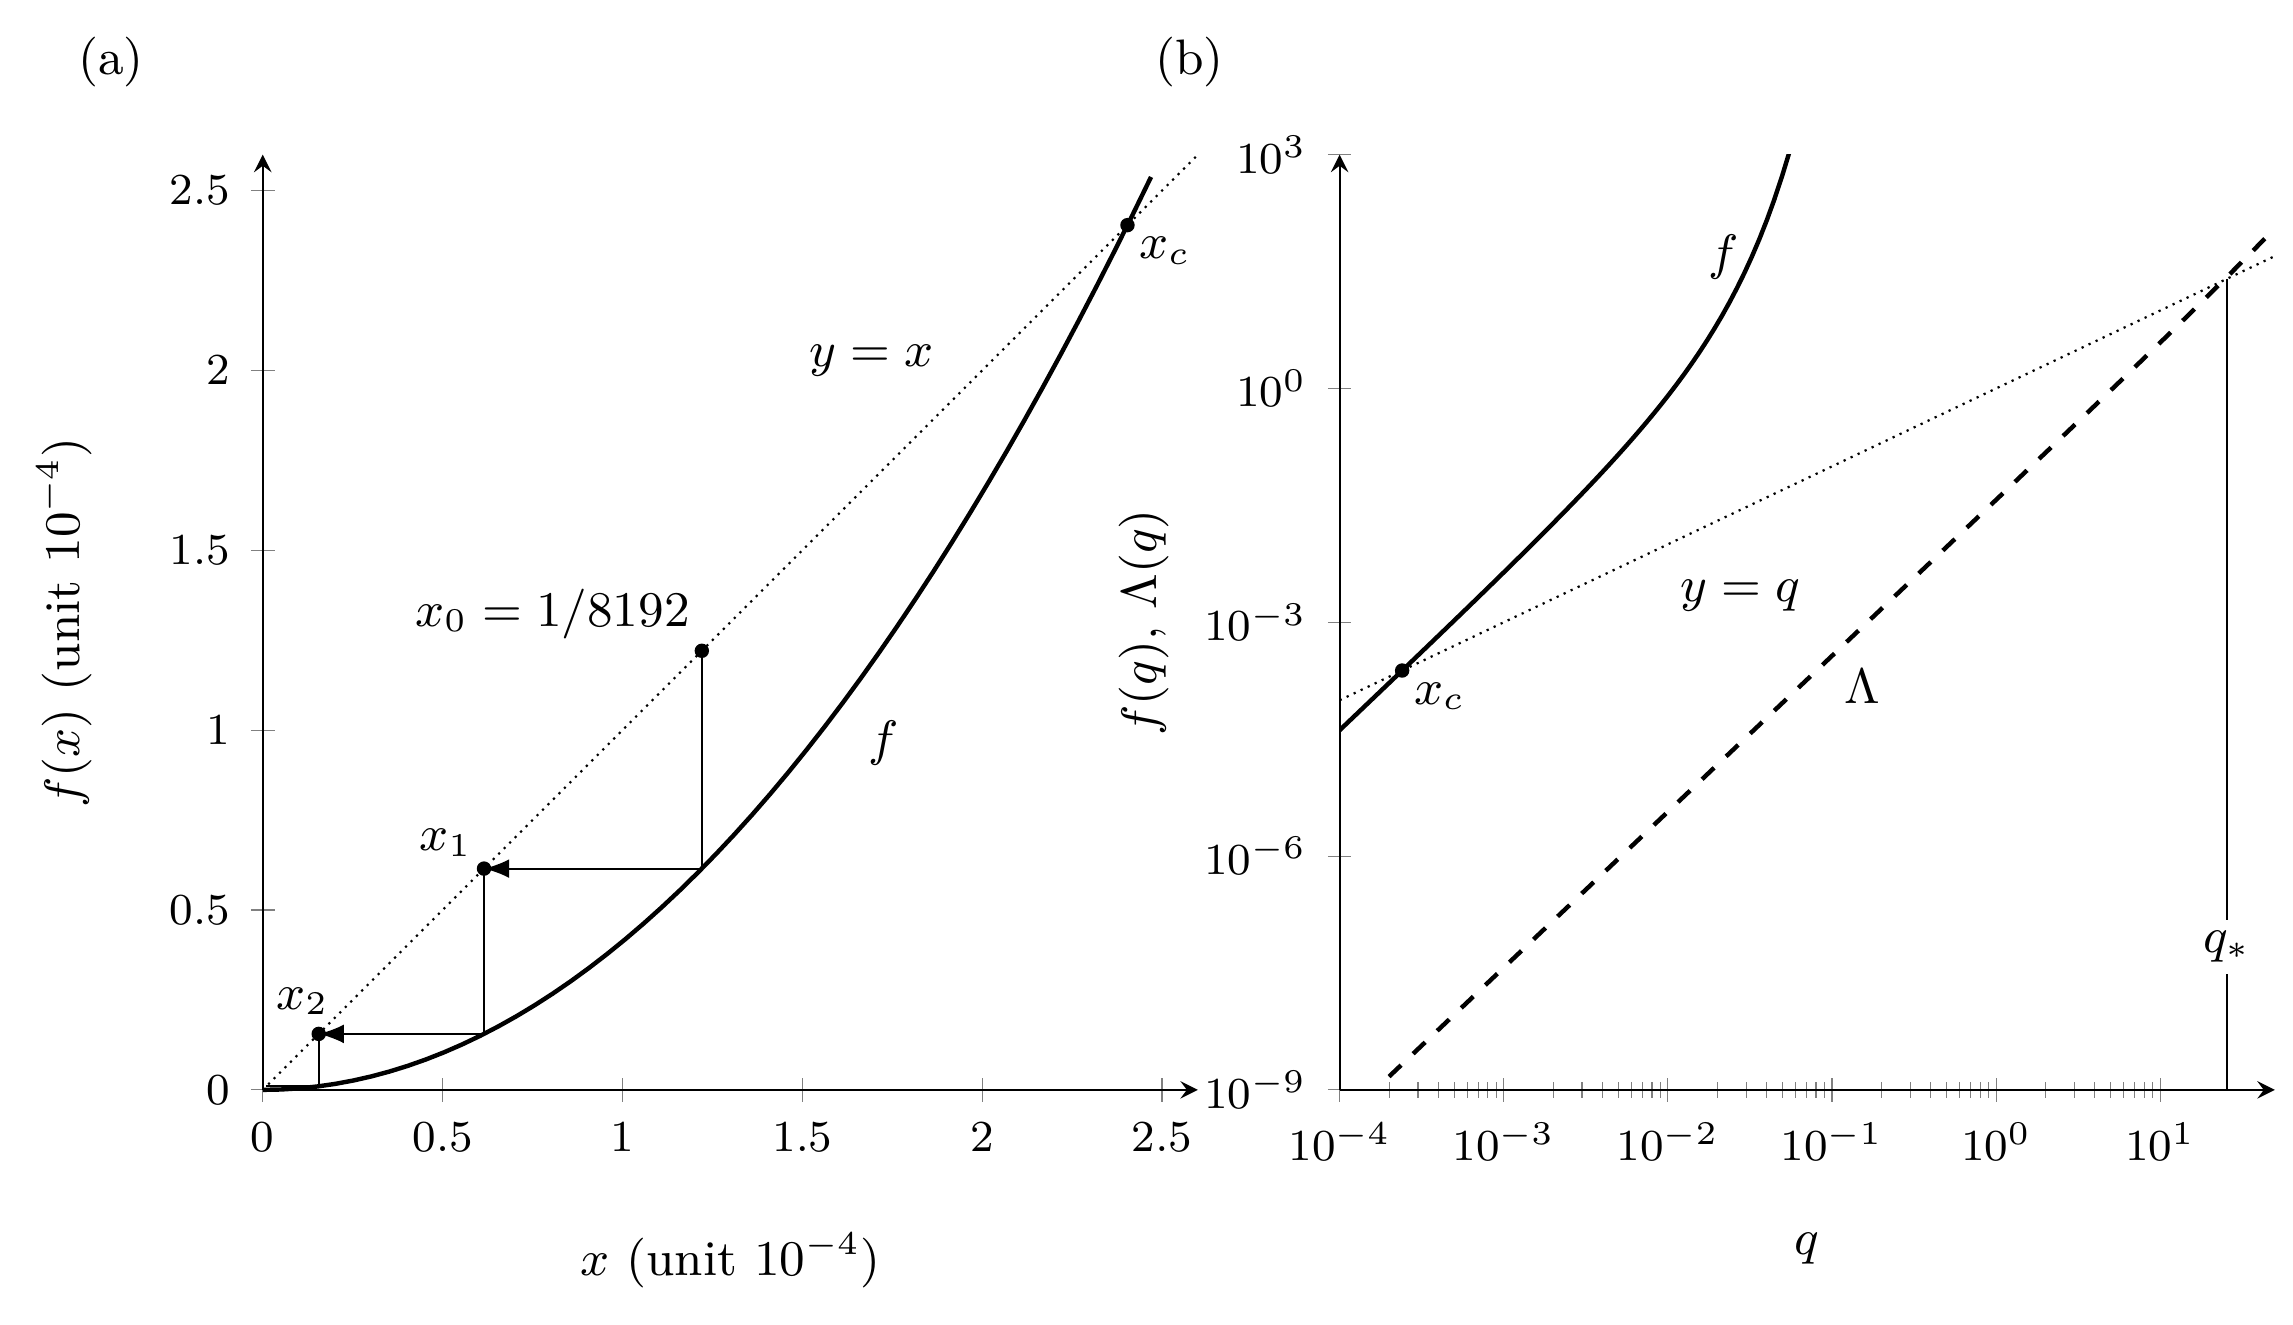
\includegraphics[width=412.7bp]{figures/fig03.png}
\caption{The ascent map $f(x)=(e^{64x}-1)^2$. (a)~Linear axes in units of $10^{-4}$: the graph of $f$, the diagonal (dotted) and the cobweb of the first iterates from $x_0=\xconstinl$; every start below the fixed point $x_c\in(1/4160,1/4159)$ is driven to $0$ (\cref{thm:ascent,thm:zero-one}). (b)~Logarithmic axes: $f$ (solid), the lower bound $\Lambda$ of \cref{thm:universal-step} for any step $X(T_{k+1})\le\Phi(X(T_k))$ valid in every \PSTS{} at $T_0=3$ (dashed), and the diagonal (dotted). Every such step satisfies $\Phi(q)\ge q$ for $q\ge q_*=216\log\frac98$, so none contracts there.}
\label{fig:ascent}
\end{figure}

\noindent\emph{Remark.} (i) \Bstar{} at $T_0$ implies \Bcirc{} at $T_0$: the cube $c_0$ lies in $\Wwin_{T_0}$, so $X(T_0)\le8\gamma T_0^3=4y_0/96^3\le1/(5\cdot96^3)=1/4\,423\,680$. Conversely, \Bcirc{} at $T_0$ implies \Bstar{} at $16T_0=T_4$: by \cref{thm:ascent}(a), $X(T_4)\le x_4=v_3^2\le u^{16}/4096$, and $u^{16}<2\cdot10^{-5}<1/8640$, so $X(T_4)<1/(4096\cdot8640)=1/35\,389\,440$, and \cref{cor:window-datum}(a) applies at $T_4$. (ii) For cubes of side $n\ge2T_0$, \Bcirc{} therefore gives the conclusions (b) and (c) of \cite[Theorem~7]{bhattacharjee2026first} with $u_0$ replaced by $32/63$, so the gap constant $0.172$ becomes $0.677$, and with the prefactor $1.9\cdot10^{-11}$ replaced by $1/4096$. (iii) The window condition \eqref{ms:eq:rational-condition} implies \Mcirc{} at $T_0$, because at $s=c_0$ it reads $\psiT{c_0}{T_0}\le1/2\,225\,664\le\dconstinl$. The tolerance of \Mcirc{} is more than $543$ times larger, and \Mcirc{} involves one torus pair instead of all shapes of $\Wwin_{T_0}$.\footnote{The argument of \cite[Theorem~7]{bhattacharjee2026first} with $96$, $24$, $13\,824$ replaced by $80$, $20$, $8000$, using \cite[Proposition~26]{bhattacharjee2026first} at $P=20T$, accepts on the window $\{s:2T_0\le s_j<40T_0\}$ the coefficient $\Vol{s}/(13\,510\,000\,T_0^3)$ in place of $\Vol{s}/(161(48T_0)^3)$, an allowance $1.318$ times larger, with the gap constant $\log(80724/80645)<10^{-3}$. At the cube it asks $\psiT{c_0}{T_0}\le1/1\,688\,750$. This variant is not proved or used here.}

A gap on the dyadic cubes allows a much larger tolerance at the base scale. The gap must then also be assumed on the target cube, which in general is not dyadic.

\begin{theorem}[gap on dyadic cubes and one cube]\label{thm:dyadic-gap}
Let $T_0\ge3$, $T_i=2^iT_0$, $\delta>0$ and $\xi>0$, and suppose:
\begin{enumerate}[label=(\roman*)]
\item $r_1\le e^{-\delta}$ on the cubes $\cube{T_i}$ for every $i\ge1$;
\item $X(T_0)\le\xi$ and $\vartheta:=e^{-\delta T_0}(e^{64\xi}-1)/\xi\le1$.
\end{enumerate}
Then for every $i\ge0$
\[
X(T_i)\le\xi\,\vartheta^{\,i}e^{-\delta(T_i-(i+1)T_0)}\le\xi,
\]
and $\log\Zs{t}{T_i}\le X(T_i)\Vol{t}/T_i^3$ for every spatial torus $t$ with all sides at least $2T_i$.
If moreover a cube $n^3$ with $2T_i\le n<4T_i$ for some $i\ge0$ satisfies $r_1(n^3)\le e^{-\delta}$, then $\Zs{n^3}{n}-1\le e^{-\delta n/2}(e^{64\xi}-1)$. For $\xi=1/10$ the condition $\vartheta\le1$ reads $\delta T_0\ge\log(10(e^{6.4}-1))$, which holds if $\delta T_0\ge8.71$. In particular, the gap $r_1\le e^{-\delta}$ on the cubes $\cube{T_i}$, $i\ge1$, and on the target cube $n^3$, $n\ge2T_0$, together with $X(T_0)\le1/10$ and $\delta T_0\ge8.71$, gives $\Zs{n^3}{n}-1\le e^{-\delta n/2}(e^{6.4}-1)$.
\end{theorem}

\begin{proof}
Induction on $i$, the case $i=0$ being (ii). Let $s=\cube{T_{i+1}}=(4T_i)^3$. By \eqref{eq:cube-control}, $\Dexc{s}{T_i}\le e^{64X(T_i)}-1$, and by \eqref{eq:gap-step} with the gap on $s$, $X(T_{i+1})\le\Dexc{s}{2T_i}\le e^{-\delta T_i}\Dexc{s}{T_i}$. The function $x\mapsto(e^{64x}-1)/x$ is increasing on $(0,\infty)$ and $X(T_i)\le\xi$, so
\[
X(T_{i+1})\le e^{-\delta T_i}\,\frac{e^{64\xi}-1}{\xi}\,X(T_i)=\vartheta\,e^{-\delta(T_i-T_0)}X(T_i)\le X(T_i),
\]
and $\sum_{j<i}(T_j-T_0)=T_i-(i+1)T_0\ge0$ gives the displayed bound. The bound on $\log\Zs{t}{T_i}$ is \eqref{eq:cube-control}. For the cube, $n^3/T_i^3<64$, so $\Dexc{n^3}{T_i}\le e^{64X(T_i)}-1\le e^{64\xi}-1$ by \eqref{eq:cube-control}; $n-T_i\ge n/2$ because $n\ge2T_i$; and \eqref{eq:gap-step} with the gap on $n^3$ gives $\Dexc{n^3}{n}\le e^{-\delta(n-T_i)}\Dexc{n^3}{T_i}\le e^{-\delta n/2}(e^{64\xi}-1)$. Finally $10(e^{6.4}-1)<6008.5<e^{8.71}$.
\end{proof}

For a continuum family (\cref{def:continuum-family}) with $\delta=\Delta/N$ and $n=N\Lp$ the last bound reads $\Zc_{N,p}-1\le e^{-\Delta\Lp/2}(e^{6.4}-1)$, where $\Zc_{N,p}=\Zs{(N\Lp)^3}{N\Lp}$ at the coupling $\betaNp$, as in \cref{thm:main}. The first paper \cite[Theorem~6]{bhattacharjee2026first} obtained the same type of bound from the gap on all tori of aspect ratio less than $24$ with sides in $[2T_i,48T_i)$ and a density bound on the whole window, under $\Delta\tzero\ge\log(16(e-1))$. \Cref{thm:dyadic-gap} replaces these by the gap on the dyadic cubes and on the target cube and by one number $X(T_0)\le1/10$, at the price of the stronger condition $\delta T_0\ge8.71$. Without any gap hypothesis, \cref{thm:ascent} needs $\xconstinl$ in place of $1/10$.

\subsection{The zero--one law}

Two one-step bounds hold in every \PSTS{}: for integers $T'\ge T\ge3$,
\begin{equation}\label{eq:one-step}
X(T')\le8\Bigl(\frac{T'}{T}\Bigr)^3X(T),\qquad X(2T)\le f\bigl(X(T)\bigr).
\end{equation}
For the first, the cube $\cube{T'}$ has sides at least $2T$, so \eqref{eq:cube-control} gives $\log\Zs{\cube{T'}}{T}\le8(T'/T)^3X(T)$, and $\Zs{\cube{T'}}{T'}\le\Zs{\cube{T'}}{T}$ because $T'\ge T$. The second is the induction step in the proof of \cref{thm:ascent}(a) with $X(T)$ in place of $x_i$: for $s=(4T)^3$, $\Dexc{s}{T}\le e^{64X(T)}-1$, and $X(2T)=\log\Zs{s}{2T}\le\Dexc{s}{2T}\le\Dexc{s}{T}^2$.

Let $(Z_{N,p})$ be a family of \PSTS{} indexed by integers $N,p\ge1$,\footnote{$N$ may run through an infinite set of positive integers, such as the arithmetic progression of \cref{def:continuum-family}; the proofs below are pointwise in $(N,p)$ and do not change.} and let $X_{N,p}(T)$ be $X(T)$ computed in $Z_{N,p}$. As in \cref{sec:psts}, \Mcirc{} holds \emph{along the family} with $\tzero>0$ if for every sufficiently large $p$ there is $N_0(p)$ such that for every $N\ge N_0(p)$ the system $Z_{N,p}$ satisfies \Mcirc{} at some integer $T_0$ with $3\le T_0\le N\tzero$; the same convention is used for \Bcirc{}. For the continuum family of \cref{def:continuum-family}, $Z_{N,p}$ is the Wilson system at $\betaNp$, and this is \Mcirc{} along the tuning. The cube datum involves no $\Lp$; if $Z_{N,p}$ does not depend on $p$, the quantifier over $p$ is void. For $t>0$ put
\[
y(t)=\limsup_{p\to\infty}\,\limsup_{N\to\infty}\,X_{N,p}(\lfloor Nt\rfloor)\in[0,\infty],
\]
the free energy of the cube of physical side $2t$ at the temperature $1/t$, measured along the family.

\begin{theorem}[zero--one law]\label{thm:zero-one}
The map $f$ has exactly one fixed point $x_c$ in $(0,\infty)$, and $x_c\in(1/4160,1/4159)$; moreover $f(x)<x$ on $(0,x_c)$ and $f(x)>x$ on $(x_c,\infty)$.
\begin{enumerate}[label=(\alph*)]
\item In every \PSTS{}, if $X(T_0)\le\xconstinl$ for an integer $T_0\ge3$, then $X(T)<u^{T/(2T_0)}/64$ for every integer $T\ge T_0$.
\item For every $c\in(0,x_c)$ there is an integer $i_0(c)\ge0$ with $f^{i_0(c)}(c)\le\xconstinl$. In every \PSTS{}, if $X(T_1)\le c$ for an integer $T_1\ge3$, then $X(2^{i_0(c)}T_1)\le\xconstinl$, and hence $X(T)<u^{T/(2^{i_0(c)+1}T_1)}/64$ for every integer $T\ge2^{i_0(c)}T_1$.
\item For a family $(Z_{N,p})$ as above, exactly one of the following holds:
\begin{enumerate}[label=(\Roman*)]
\item $y(t)\ge x_c$ for every $t>0$;
\item there is $\tzero>0$ such that $y(t)\le u^{t/(2t_0)}/64=e^{-\Delta t/2}/64$ for every $t>\tzero$, where $\Delta=\tzero^{-1}\log\frac{63}{32}$.
\end{enumerate}
The following are equivalent: \textup{(II)}; \Mcirc{} along the family; \Bcirc{} along the family; $\lim_{t\to\infty}y(t)=0$; $y(t_1)<x_c$ for some $t_1>0$. If \Mcirc{} or \Bcirc{} holds along the family with $\tzero$, then \textup{(II)} holds with the same $\tzero$. In particular, if $y(t)\to0$ then $t^ay(t)\to0$ for every $a>0$: $y$ cannot tend to $0$ at only a power-law rate.
\end{enumerate}
\end{theorem}

\begin{proof}
The functions $x\mapsto(e^{64x}-1)/x$ and $x\mapsto e^{64x}-1$ are positive and strictly increasing on $(0,\infty)$, and the second tends to $0$ as $x\downarrow0$. So $f(x)/x$, their product, increases strictly from $0$ to $\infty$. Hence $f$ has one positive fixed point $x_c$, with $f(x)<x$ below it and $f(x)>x$ above it. The comparisons $f(1/4160)<1/4160$ and $f(1/4159)>1/4159$ are certificates of \cref{app:certificates}.

(a) Let $T_i=2^iT_0$ and $x_i$, $v_i$ be as in \cref{thm:ascent}. By the second bound of \eqref{eq:one-step}, the monotonicity of $f$ and induction, $X(T_i)\le x_i$. Further $64x_0=1/128\le1/126=u/64$, and for $i\ge1$, $64x_i=64v_{i-1}^2\le64(u^{2^{i-1}}/64)^2=u^{2^i}/64$ by \cref{thm:ascent}(a). So
\begin{equation}\label{eq:envelope}
64x_i\le\frac{u^{2^i}}{64}\qquad(i\ge0).
\end{equation}
For $T\in[T_i,T_{i+1})$ the first bound of \eqref{eq:one-step} gives $X(T)\le8(T/T_i)^3X(T_i)\le64x_i\le u^{2^i}/64$, and $u^{2^i}<u^{T/(2T_0)}$ because $T/(2T_0)<2^i$ and $u<1$.

(b) Since $f$ is increasing and $f(x)<x$ on $(0,x_c)$, the iterates $f^i(c)$ decrease and stay positive. Their limit is a fixed point of $f$ in $[0,c]$, hence $0$, so $i_0(c)$ is well defined. By the second bound of \eqref{eq:one-step}, the monotonicity of $f$ and induction, $X(2^iT_1)\le f^i(c)$; in particular $X(2^{i_0(c)}T_1)\le\xconstinl$. The last claim is (a) with $T_0=2^{i_0(c)}T_1$.

(c) We prove the cycle \Mcirc{} $\Rightarrow$ \Bcirc{} $\Rightarrow$ (II) $\Rightarrow$ $\lim y=0$ $\Rightarrow$ \Mcirc{}, keeping $\tzero$ in the first two steps, and the implications $\lim y=0\Rightarrow y(t_1)<x_c$ for some $t_1$ $\Rightarrow$ \Bcirc{}.

\Mcirc{} along the family with $\tzero$ implies \Bcirc{} with the same $\tzero$, by \cref{lem:purity-conversion}.

Suppose \Bcirc{} along the family with $\tzero$. For all large $p$ and $N\ge N_0(p)$ there is $T_0\le N\tzero$ with $X_{N,p}(T_0)\le\xconstinl$. Let $t>\tzero$. If $N\ge1/(t-\tzero)$, then $\lfloor Nt\rfloor\ge Nt-1\ge N\tzero\ge T_0$, and by (a)
\[
X_{N,p}(\lfloor Nt\rfloor)<\frac{u^{\lfloor Nt\rfloor/(2T_0)}}{64}\le\frac{u^{(Nt-1)/(2N\tzero)}}{64}.
\]
Letting $N\to\infty$ and then $p\to\infty$ gives $y(t)\le u^{t/(2\tzero)}/64$, which is (II) with the same $\tzero$; and $u^{t/(2t_0)}=e^{-\Delta t/2}$.

(II) implies $\lim_{t\to\infty}y(t)=0$, which implies $y(t_1)<x_c$ for some $t_1$.

Suppose $\lim_{t\to\infty}y(t)=0$, and choose $t_1$ with $y(t_1)<1/8194$. There is $p_0$ such that $\limsup_NX_{N,p}(\lfloor Nt_1\rfloor)<1/8194$ for $p\ge p_0$, and then $N_0(p)$ such that $X_{N,p}(\lfloor Nt_1\rfloor)<1/8194$ and $\lfloor Nt_1\rfloor\ge3$ for $N\ge N_0(p)$. By \eqref{eq:X-psi}, $T_0=\lfloor Nt_1\rfloor\le Nt_1$ satisfies $\psiT{\cube{T_0}}{T_0}\le2X_{N,p}(T_0)<2/8194=\dconstinl$. This is \Mcirc{} along the family with $\tzero=t_1$.

Suppose $y(t_1)<x_c$, and choose $c$ with $y(t_1)<c<x_c$. As in the previous step, for $p\ge p_0$ and $N\ge N_0(p)$ the integer $T_1=\lfloor Nt_1\rfloor\ge3$ satisfies $X_{N,p}(T_1)<c$. By (b), $X_{N,p}(2^{i_0(c)}T_1)\le\xconstinl$ with $3\le2^{i_0(c)}T_1\le N2^{i_0(c)}t_1$. This is \Bcirc{} along the family with $\tzero=2^{i_0(c)}t_1$.

So the five statements are equivalent. Alternative (I) is the negation of the last of them, so exactly one of (I) and (II) holds. If $y(t)\to0$, then (II) holds, and $y(t)\le e^{-\Delta t/2}/64$ for $t>\tzero$ gives $t^ay(t)\to0$.
\end{proof}

\noindent\emph{Remark.} Both alternatives occur among families of \PSTS{}. For $0<q<1$ the function $Z(n)=1+q^{|n|}$ is a \PSTS{} with $\TT_s=\mathrm{diag}(1,q^{\Vol{s}})$ (\cref{prop:gapless-sector}), so $\Zs{s}{T}=1+q^{\Vol{s}T}$ and $X(T)=\log(1+q^{8T^4})$. A fixed $q$ gives $X(\lfloor Nt\rfloor)\to0$, hence $y\equiv0$ and alternative (II). The choice $q_N=e^{-N^{-5}}$ gives $X_N(\lfloor Nt\rfloor)=\log\bigl(1+e^{-8\lfloor Nt\rfloor^4/N^5}\bigr)\to\log2$, because $\lfloor Nt\rfloor^4/N^5\le t^4/N$; so $y\equiv\log2>x_c$ and alternative (I) holds. No property of these systems beyond (P1) and (P2) is claimed. For the Wilson theory along the continuum tuning it is not known which alternative holds.

\subsection{Upward closure and decimation}

The ascent also shows that the set of scales at which the datum holds is closed upwards, up to a factor $8$, and decimation identifies the datum at $T_0=3b$ with the smallest cube of a coarser system.

\begin{theorem}[upward closure and decimation]\label{thm:upward-closed}
Let $Z$ be a \PSTS{}, $T_0\ge3$, $T_i=2^iT_0$, and let $x_i$ be as in \cref{thm:ascent}.
\begin{enumerate}[label=(\alph*)]
\item If $X(T_0)\le\xconstinl$, in particular if $Z$ satisfies \Mcirc{} at $T_0$, then $X(T)\le64x_i$ for every $i\ge0$ and every integer $T\in[T_i,2T_i)$. The sequence $(x_i)$ decreases, $64x_0=1/128$, and
\[
64x_1\le3.968\cdot10^{-3},\qquad64x_2\le1.0157\cdot10^{-3},\qquad64x_3\le6.6164\cdot10^{-5}.
\]
Consequently every integer $T\ge8T_0$ satisfies $X(T)\le6.6164\cdot10^{-5}<\xconstinl$ and $\psiT{\cube{T}}{T}\le1.3233\cdot10^{-4}<\dconstinl$: $Z$ satisfies \Mcirc{} and \Bcirc{} at every integer $T\ge8T_0$.
\item Let $b\ge1$ and let $Z^{[b]}$ be the decimated system of \cref{thm:decimation}, with $X^{[b]}_{s'}(T')=\log\Zc^{[b]}_{s'}(T')$. For every $k\ge0$, $X(T_k)=X^{[2^k]}_{\cube{T_0}}(T_0)$, and if $b$ divides $T_0$ with $T_0/b\ge3$, then $X(T_k)=X^{[b]}_{(2T_k/b)^3}(T_k/b)$. For $T_0=3b$:
\[
\text{\Mcirc{} at }T_0\iff\psi^{[b]}_{6^3}(3)\le\dconstinl,\qquad\text{\Bcirc{} at }T_0\iff X^{[b]}_{6^3}(3)\le\xconstinl,
\]
and $\psi^{[b]}_{6^3}(3)\le\dconstinl\Rightarrow X^{[b]}_{6^3}(3)\le\xconstinl\Rightarrow\psi^{[b]}_{6^3}(3)\le1/4096$. If $X^{[b]}_{6^3}(3)\le\xconstinl$, then in $Z$ every cube of side $n\ge6b$, divisible by $b$ or not, has $r_1(n^3)\le u^{1/(3b)}$ and $\Zs{n^3}{n}-1\le u^{n/(6b)}/4096$. For every blocked system $c^{|n|}Z(bn)$ of \cref{thm:decimation}(b) the quantities $X^{[b]}$ and $\psi^{[b]}$ are unchanged.
\item A family $(Z_{N,p})$ as in \cref{thm:zero-one} satisfies \Bcirc{} along the family if and only if there is $t_1>0$ such that for every sufficiently large $p$ and every $N\ge N_0(p)$ some integer $b$ with $1\le b\le Nt_1$ has $X^{[b]}_{6^3}(3)\le\xconstinl$ in $Z_{N,p}^{[b]}$. By \cref{thm:zero-one}(c) this is also equivalent to \Mcirc{} along the family.
\end{enumerate}
\end{theorem}

\begin{proof}
(a) Let $T\in[T_i,2T_i)$ and $t=\cube{T}$. All sides of $t$ are at least $2T_i$ and $\Vol{t}/T_i^3=8T^3/T_i^3<64$. By \cref{thm:ascent}(a), $\log\Zs{t}{T_i}\le64x_i$, and $\Zs{t}{T}\le\Zs{t}{T_i}$ since $T\ge T_i$; so $X(T)\le64x_i$. Since $0<x_0<x_c$ and $f$ is increasing with $0<f(x)<x$ on $(0,x_c)$ (\cref{thm:zero-one}), $(x_i)$ decreases. For the numbers we use $e^y-1\le y+y^2$ for $0\le y\le1$, which holds because $\sum_{k\ge2}y^k/k!\le(e-2)y^2$; then $64x_{i+1}=64(e^{64x_i}-1)^2\le64(y_i+y_i^2)^2$ whenever $64x_i\le y_i\le1$. From $y_0=1/128$, $64x_1\le64(129/16\,384)^2=16\,641/4\,194\,304<3.968\cdot10^{-3}$. From $y_1=3.968\cdot10^{-3}$, $64x_2\le1.0157\cdot10^{-3}$, and from $y_2=1.0157\cdot10^{-3}$, $64x_3\le6.6164\cdot10^{-5}$; both are exact rational comparisons. If $T\ge8T_0$, then $T\in[T_i,2T_i)$ with $i\ge3$, so $X(T)\le64x_i\le64x_3\le6.6164\cdot10^{-5}<\xconstinl$, and $\psiT{\cube{T}}{T}\le2X(T)\le1.3233\cdot10^{-4}<\dconstinl$ by \eqref{eq:X-psi}.

(b) By \cref{thm:decimation}(a), $\Zc^{[b]}_{s'}(T')=\Zs{bs'}{bT'}$ for $T'\ge2$ and $\psi^{[b]}_{s'}(T')=\psiT{bs'}{bT'}$ for $T'\ge3$. With $b=2^k$, $s'=\cube{T_0}$ and $T'=T_0$ this gives $X^{[2^k]}_{\cube{T_0}}(T_0)=X(T_k)$. If $b$ divides $T_0$ and $T_0/b\ge3$, the cube $(2T_k/b)^3$ at time $T_k/b$ lies in the domain of $Z^{[b]}$, and $s'=(2T_k/b)^3$, $T'=T_k/b$ give the second identity. For $T_0=3b$, $s'=6^3$ and $T'=3$ give $\psi^{[b]}_{6^3}(3)=\psiT{c_0}{T_0}$ and $X^{[b]}_{6^3}(3)=X(T_0)$, which are the two equivalences; the chain of implications is \cref{lem:purity-conversion} and \eqref{eq:X-psi}. If $X(3b)\le\xconstinl$, \cref{thm:ascent}(b),(c) applied to $Z$ at $T_0=3b$ give the bounds on every cube of side $n\ge6b$; through $Z^{[b]}$ one reaches only sides divisible by $b$. By \cref{thm:decimation}(b) the multiplier $c^{|n|}$ of an exact blocking does not change $\Zc$ or $\psi$, so the blocked system has the same normalised quantities as $Z^{[b]}$. This is the identity of \cref{ms:prop:RG-defect} with vanishing remainder.

(c) Suppose \Bcirc{} along the family with $\tzero$: for all large $p$ and $N\ge N_0(p)$ some $3\le T_0\le N\tzero$ has $X_{N,p}(T_0)\le\xconstinl$. Let $b=\lceil8T_0/3\rceil$, so $8T_0\le3b\le8T_0+2$. By (a), $X_{N,p}(3b)\le\xconstinl$, which by (b) is $X^{[b]}_{6^3}(3)\le\xconstinl$; and $b\le(8N\tzero+2)/3\le3N\tzero$ because $N\tzero\ge T_0\ge3$. So the condition holds with $t_1=3\tzero$. Conversely, if $1\le b\le Nt_1$ and $X^{[b]}_{6^3}(3)\le\xconstinl$, then $T_0=3b$ satisfies $3\le T_0\le3Nt_1$ and $X_{N,p}(T_0)\le\xconstinl$ by (b); this is \Bcirc{} along the family with $\tzero=3t_1$.
\end{proof}

The factor $8$ in (a) cannot be removed by this argument: $64x_0=1/128$, $64x_1\ge1/256$ and $64x_2\ge1/1024$, all larger than $\xconstinl$, so the bound gives nothing below $\xconstinl$ at the scales $T$ with $T_0<T<8T_0$. In (b) the two forms of the datum cannot be identified at one scale. For $0<r<1$ the product of rings $Z(n)=\prod_{\mu=1}^4(1+r^{n_\mu})^{|n|/n_\mu}$ is a \PSTS{} with $\Zs{s}{T}=(1+r^T)^{\Vol{s}}$ (\cref{thm:universal-step}(a) with $m=1$). At $T_0=3$, $b=1$ and $\rho=r^3=1/1\,769\,473$, one has $X(3)=216\log(1+\rho)\le216\rho<216/1\,769\,472=\xconstinl$, while $\psiT{6^3}{3}=432\log(1+\rho)-216\log(1+\rho^2)\ge432\rho(1-\rho)>\dconstinl$. The bound $\psiT{6^3}{3}\ge432\rho(1-\rho)$ uses $\log(1+\rho)\ge\rho-\rho^2/2$ and $\log(1+\rho^2)\le\rho^2$, and $432\rho(1-\rho)>\dconstinl$ is $4097\cdot432\cdot1\,769\,472>1\,769\,473^2$, which holds because $4097\cdot432=1\,769\,904$.
\section{The continuum conclusion from one cube}\label{sec:continuum}

The lattice theorems of \cref{sec:ascent} concern one Wilson system at a time. This section passes to continuum limits along a continuum family in the sense of the first paper \cite{bhattacharjee2026first}: the mesh tends to zero first and the physical side of a symmetric torus tends to infinity second. On the family we assume either the uniform ultraviolet bound \UVB{} on separated smears or the hypothesis \hypW{} of the first paper; in the main theorem only the convergence clauses of \hypW{} are used. The main result, \cref{thm:main}, shows that \Mcirc{} along the tuning gives every limit a spectral gap of at least $\Delta=\tzero^{-1}\log\frac{63}{32}$ above a unique vacuum.

\subsection{Continuum families and the two hypotheses}

For integers $L,M\ge3$ let $\Lambda_{L,M}=\Lambda(n)$ with $n=(L^3,M)$, and let $\mu_{L,M}$ be the Wilson probability measure $W_n(U)\prod\dd U/Z(n)$ of \eqref{eq:wilson-weight} on it, at the coupling under consideration. We write $x^0$ for the time coordinate of a site or of a point of $\R^4$, $e_0$ for the unit vector in the time direction, and $(x,0)$ for the temporal link from $x$ to $x+e_0$.

\begin{definition}[{continuum family; \cite[Definition~3]{bhattacharjee2026first}}]\label{def:continuum-family}
Fix a closed subgroup $G\subset\U(N_c)$. A \emph{continuum family} consists of lattice spacings $\aN=1/N$, $N\in\Nat$, physical sides $\Lp\in\Nat$ with $\Lp\to\infty$, couplings $\betaNp\ge0$, a countable set $V$ of \emph{tokens}, and, for all $N$, $p$ and $v\in V$, a complex function $\Phi^{N,p}_v(x,Q)$ of a site $x$ of $\Lambda_{N\Lp,M}$ and a configuration $Q$, given for every $M$ by the same formula, such that:
\begin{enumerate}[label=(F\arabic*),leftmargin=3em]
\item $\Phi^{N,p}_v(x,\cdot)$ is continuous, gauge invariant, and depends only on the links in $x+R_v$ for a finite set $R_v\subset\Z^4$ independent of $N$ and $p$;
\item $\Phi^{N,p}_v(x+y,Q)=\Phi^{N,p}_v(x,\tau_{-y}Q)$ for every site $y$, where $(\tau_yQ)_{(x,\mu)}=Q_{(x-y,\mu)}$;
\item there is an involution $v\mapsto v^\vartheta$ of $V$ with $\Phi^{N,p}_{v^\vartheta}(x,Q)=\overline{\Phi^{N,p}_v(\vartheta x,\vartheta Q)}$, where $\vartheta$ reverses the time coordinate and acts on configurations by $(\vartheta Q)_{(x,j)}=Q_{(\vartheta x,j)}$ for spatial links and $(\vartheta Q)_{(x,0)}=Q_{(\vartheta x-e_0,0)}^{-1}$ for temporal links.
\end{enumerate}
\end{definition}

The insertions may carry renormalisation constants depending on $N$; no bound on $\sup\abs{\Phi^{N,p}_v}$ uniform in $N$ is assumed. The map $\vartheta$ preserves $\mu_{L,M}$ for all $L,M$, because it maps plaquettes to plaquettes up to inversion and preserves Haar measure.

For $m\ge1$ let $D_m\subset(\R^4)^m$ be the open set of $m$-tuples of pairwise distinct points. For compact $K\subset D_m$ let $C^\infty_c(K)$ be the space of smooth complex functions with support in $K$, with the norms $\norm{t}_{C^k}=\max_{\abs{\alpha}\le k}\sup\abs{\partial^\alpha t}$, which increase with $k$ and make $C^\infty_c(K)$ a Fr\'echet space. A \emph{cluster} is a pair $(v,t)$ with $v\in V^m$ and $t\in C^\infty_c(D_m)$. For a cluster supported in the box $\bigl((-\Lp/2,\Lp/2)^3\times(-M/2N,M/2N)\bigr)^m$ the lattice smear on $\Lambda_{N\Lp,M}$ is
\begin{equation}\label{eq:cont-smear}
S_{N,p,M}(v,t)=\aN^{4m}\sum_{x_1,\dots,x_m}t(\aN x_1,\dots,\aN x_m)\,\mu_{N\Lp,M}\Bigl(\prod_{i=1}^m\Phi^{N,p}_{v_i}(x_i,\cdot)\Bigr),
\end{equation}
the sum running over sites, with $\aN x$ read in the box. We write $\mu_{N\Lp}=\mu_{N\Lp,N\Lp}$ for the symmetric torus and $S_{N,p}=S_{N,p,N\Lp}$. In physical units
\begin{equation}\label{eq:physical-units}
\aN=\frac1N,\qquad N\Lp\cdot\aN=\Lp,\qquad \Tzero\aN\le\tzero\quad\text{when}\quad3\le\Tzero\le N\tzero ,
\end{equation}
so the symmetric torus has physical side $\Lp$ in all four directions and carries the coupling $\betaNp$, and \Mcirc{} along the tuning with $\tzero$ (\cref{sec:psts}) is a statement about the Wilson system at $\betaNp$ on a cube of physical side $2\Tzero\aN\le2\tzero$ at inverse temperature $\Tzero\aN\le\tzero$.

\begin{definition}[{hypothesis \hypW; quoted from \cite[Definition~4]{bhattacharjee2026first} with the notation adapted}]\label{def:W}
A continuum family satisfies \hypW{} if there are a compact metric space $X$ of phases with a Borel probability measure $\nu$ of full support, and for every $\chi\in X$ and every cluster a number $S^\chi(v,t)=\int tS^\chi_v$ with $S^\chi_v$ a smooth function on $D_m$, continuous in $\chi$ at every point of $D_m$, such that for every cluster
\[
\lim_{p\to\infty}\lim_{N\to\infty}S_{N,p,N\Lp}(v,t)=\int_XS^\chi(v,t)\dd\nu(\chi),
\]
with $\chi\mapsto S^\chi(v,t)$ $\nu$-integrable, the inner limit along $N$ in an arithmetic progression and the outer along a sequence of $p$, and for every $\chi$ outside a $\nu$-null set the functions $S^\chi_v$ are the Schwinger functions of a Wightman theory with a unique vacuum, in the sense of \cite[Section~7.5 and Lemma~13]{bhattacharjee2026first}, in which the field of $v^\vartheta$ is the adjoint of the field of $v$.
\end{definition}

We call the progression $\mathcal P$ and the sequence $(p_j)$ those of \hypW{} and write $\bar S(v,t)=\int_XS^\chi(v,t)\dd\nu(\chi)$. The \emph{convergence clauses} of \hypW{} are the displayed iterated limit and the integrability of $\chi\mapsto S^\chi(v,t)$.

\begin{definition}[uniform ultraviolet bound]\label{def:UVB}
A continuum family satisfies \UVB{} if for every $m\ge1$, every $v\in V^m$ and every compact $K\subset D_m$ there are $k\in\Nat$, $C<\infty$, $p_K$ and $N_K(p)$ such that
\[
\abs{S_{N,p}(v,t)}\le C\norm{t}_{C^k}\qquad\text{for all }t\in C^\infty_c(K),\ p\ge p_K,\ N\ge N_K(p).
\]
\end{definition}

\begin{remark}
If $\abs{\Phi^{N,p}_v}\le C_v$ for all $N,p,x,Q$ and every $v$, then \UVB{} holds with $k=0$ and $C=\prod_iC_{v_i}\abs{K_1}$, where $K_1$ is the sup-norm $1$-neighbourhood of $K$: the cubes $\aN x+[0,\aN)^{4m}$ over the tuples $x$ with $\aN x\in K$ are disjoint and lie in $K_1$, so $\aN^{4m}\#\{x:\aN x\in K\}\le\abs{K_1}$.
\end{remark}

\emph{Clusters as an algebra.} For a cluster $c=(v,t)$ let $F_c=\aN^{4m}\sum_xt(\aN x)\prod_i\Phi^{N,p}_{v_i}(x_i,\cdot)$, so that $S_{N,p,M}(c)=\mu_{N\Lp,M}(F_c)$. Let $\mathcal A$ be the space of finite formal linear combinations of clusters and of the empty cluster $\emptyset$, with $F_\emptyset=1$; the map $A\mapsto F_A$ and all smears are extended linearly. For $h\in\R^4$ let $\tau_hc=(v,t(\cdot-h))$, every point being translated by $h$, and $\tau_\sigma=\tau_{\sigma e_0}$. The reflected cluster is $c^\vartheta=(v^\vartheta,\Theta t)$ with $(\Theta t)(x_1,\dots,x_m)=\overline{t(\vartheta x_1,\dots,\vartheta x_m)}$, extended antilinearly to $\mathcal A$; by (F3), $F_{c^\vartheta}=\vartheta\overline{F_c}$, where $(\vartheta F)(Q)=F(\vartheta Q)$. Two clusters have the product cluster $cc'=(vv',t\otimes t')$ when $t\otimes t'$ is supported in $D_{m+m'}$, and $F_{cc'}=F_cF_{c'}$. Let $\mathcal A_+^{\delta,\omega}$ be the span of $\emptyset$ and of the clusters all of whose times lie in $(\delta,\omega)$, and $\mathcal A_+=\bigcup_{0<\delta<\omega}\mathcal A_+^{\delta,\omega}$. For $A,B\in\mathcal A_+$ and $\sigma\ge0$ the product $A^\vartheta\tau_\sigma B$ is defined, because the times of $A^\vartheta$ are negative and those of $\tau_\sigma B$ positive. For $h=\aN y$ with $y\in\Z^4$, (F2) gives $F_{\tau_hc}=\tau_yF_c$ with $(\tau_yF)(Q)=F(\tau_{-y}Q)$; we write $\tau_s=\tau_{se_0}$ for integers $s$.

Let $W_4$ be the group of signed permutations of the four coordinates. It acts on the sites of the symmetric torus $\Lambda_{N\Lp,N\Lp}$ and on configurations, by pulling back along the induced map of links, a link traversed against its orientation carrying the inverse variable, as $\vartheta\in W_4$ does in (F3). It preserves $\mu_{N\Lp}$ and maps the box $(-\Lp/2,\Lp/2)^4$ onto itself.

\subsection{Slab operators}

Fix $L\ge3$ and $\beta\ge0$, let $\TT=\TT_{L^3}$ on $\Kspace$, $\lzero$ and $\Omegazero$ be as in \cref{lem:transfer-matrix}, and let $R=\TT/\lzero$. A \emph{function of the slab} $[a,b]$, for integers $a\le b$, is a function of the spatial links at the times $a,\dots,b$ and of the temporal links from time $t$ to $t+1$ for $a\le t<b$. Let
\[
\mathfrak w(Q,U,Q')=\exp\Bigl(N_c\beta\bigl[\tfrac12S_s(Q)+\tfrac12S_s(Q')+S_0(Q,U,Q')\bigr]\Bigr)
\]
be the integrand of \eqref{eq:transfer-kernel}. For a bounded measurable function $F$ of the slab $[0,w]$ with $w\ge1$ the \emph{slab operator} $\hat F$ on $\Kspace$ has the kernel
\[
\hat F(Q_0,Q_w)=\int F(Q_0,U^{(0)},Q_1,\dots,U^{(w-1)},Q_w)\prod_{t=0}^{w-1}\mathfrak w(Q_t,U^{(t)},Q_{t+1})\prod_{t=1}^{w-1}\dd Q_t\prod_{t=0}^{w-1}\dd U^{(t)},
\]
and for $w=0$ the operator $\hat F$ is multiplication by $F$. Since $\mathfrak w>0$ and $F=1$ gives the kernel of $\TT^w$, we have $\abs{\hat F(Q,Q')}\le\norm{F}_\infty\TT^w(Q,Q')$; so $\hat F$ is Hilbert--Schmidt for $w\ge1$ and bounded for $w=0$.

\begin{lemma}[{\cite[Lemmas~11(iii)--(v), 12 and 14]{bhattacharjee2026first}}]\label{lem:gap-decay}
Let $F$ and $H$ be bounded measurable functions of the slabs $[0,w]$ and $[0,w']$, and let $M\ge3$.
\begin{enumerate}[label=(\alph*),leftmargin=2.2em]
\item \emph{Slab traces.} For $s\ge w$, $M\ge s+w'$ and $w+w'<M$,
\[
\mu_{L,M}(F\,\tau_sH)=\frac{\Tr(\hat F\TT^{s-w}\hat H\TT^{M-s-w'})}{\Tr\TT^M}.
\]
The function $\vartheta\bar F$ is a function of the slab $[-w,0]$, and for $s\ge0$ and $M\ge s+w+w'$
\[
\mu_{L,M}(\vartheta\bar F\,\tau_sH)=\frac{\Tr(\hat F^*\TT^s\hat H\TT^{M-s-w-w'})}{\Tr\TT^M}.
\]
The limit $\mu^0_L(F)=\lim_{M\to\infty}\mu_{L,M}(F)$ exists, and with $\Psi_F=\lzero^{-w}\hat F\Omegazero$,
\[
\mu^0_L(\vartheta\bar F\,\tau_sH)=\ip{\Psi_F}{R^s\Psi_H},\qquad \mu^0_L(H)=\ip{\Omegazero}{\Psi_H}\qquad(s\ge0).
\]
\item \emph{Gap to decay.} Suppose that every eigenvalue $\lambda\ne\lzero$ of $\TT$ satisfies $\lambda\le e^{-\gamma}\lzero$. Put $\Psi'_F=\Psi_F-\ip{\Omegazero}{\Psi_F}\Omegazero$ and $C_F(s)=\mu^0_L(\vartheta\bar F\,\tau_sF)-\abs{\mu^0_L(F)}^2=\ip{\Psi'_F}{R^s\Psi'_F}\ge0$. Then for all integers $s\ge s_1\ge0$
\[
\bigl\lvert\mu^0_L(\vartheta\bar F\,\tau_sH)-\overline{\mu^0_L(F)}\,\mu^0_L(H)\bigr\rvert\le e^{-\gamma(s-s_1)}\sqrt{C_F(s_1)\,C_H(s_1)} .
\]
\item \emph{Thermal discrepancy.} If $M\ge2w+2$, then $C_M(F)=\mu_{L,M}(\vartheta\bar F\,F)-\abs{\mu_{L,M}(F)}^2\ge0$, and
\[
\abs{\mu_{L,M}(F)-\mu^0_L(F)}^2\le\bigl(\Zs{L^3}{M}-1\bigr)\,C_M(F),\qquad \mu^0_L(\vartheta\bar F\,F)\le\Zs{L^3}{M}\,\mu_{L,M}(\vartheta\bar F\,F).
\]
\end{enumerate}
\end{lemma}

\begin{proof}
(a) By \cref{sec:psts}, $\sum_p\ReTr Q_p=\sum_t\bigl[S_s(Q^{(t)})+S_0(Q^{(t)},U^{(t)},Q^{(t+1)})\bigr]$; splitting each $S_s(Q^{(t)})$ into two halves writes the Wilson weight of $\Lambda_{L,M}$ as $\prod_{t\in\Z/M\Z}\mathfrak w(Q^{(t)},U^{(t)},Q^{(t+1)})$. Integrating the interior slices and the temporal links of the slab $[0,w]$ against $F$ gives $\hat F(Q_0,Q_w)$, those of $[s,s+w']$ against $\tau_sH$ give $\hat H(Q_s,Q_{s+w'})$, the remaining $s-w$ and $M-s-w'$ factors give the kernels of $\TT^{s-w}$ and $\TT^{M-s-w'}$, and the integral over the remaining slices is the trace of the composition; for $s=w$ the shared slice is the variable of the composition $\hat F\hat H$. The operator is trace class, since it contains at least two Hilbert--Schmidt factors when $M\ge3$. Dividing by $Z(n)=\Tr\TT^M$ (\cref{lem:transfer-matrix}) gives the first formula. Under $\vartheta$ the temporal link from $t$ to $t+1$ becomes the link from $-t$ to $-t-1$ traversed backwards, which is the inversion in (F3); since $S_0(Q',U,Q)=S_0(Q,U^*,Q')$ (proof of \cref{lem:transfer-matrix}(i)) and inversion preserves Haar measure, $\vartheta\bar F$ is a function of $[-w,0]$ whose translate $\tau_w(\vartheta\bar F)$ to $[0,w]$ has the kernel $\overline{\hat F(Q_w,Q_0)}=\hat F^*(Q_0,Q_w)$. Translation invariance of $\mu_{L,M}$ by $w$ steps and the first formula, applied with $s+w\ge w$, give the second. For the limit, $\lzero$ is simple and the other eigenvalues of $R$ lie in $[0,1)$ and accumulate only at $0$, so $R=P_0+S'$ with $P_0$ the projection on $\Omegazero$, $P_0S'=S'P_0=0$ and $\norm{S'}<1$. As $R^2$ is trace class, $\norm{S'^k}_1\le\norm{S'^2}_1\norm{S'}^{k-2}\to0$, hence $\Tr R^M\to1$ and $\Tr(BR^{M-c})\to\ip{\Omegazero}{B\Omegazero}$ for every bounded $B$ and fixed $c$. Applied to the first formula with $F=1$, $w=0$, $s=0$, and to the second with $B=\lzero^{-s-w-w'}\hat F^*\TT^s\hat H$, this gives $\mu^0_L(H)=\lzero^{-w'}\ip{\Omegazero}{\hat H\Omegazero}=\ip{\Omegazero}{\Psi_H}$ and $\mu^0_L(\vartheta\bar F\,\tau_sH)=\lzero^{-w-w'}\ip{\Omegazero}{\hat F^*R^s\hat H\Omegazero}=\ip{\Psi_F}{R^s\Psi_H}$.

(b) By (a), $\mu^0_L(\vartheta\bar F\,\tau_sH)=\ip{\Psi_F}{R^s\Psi_H}$. Since $R\Omegazero=\Omegazero$, $R$ is self-adjoint and $\Psi'_F,\Psi'_H\perp\Omegazero$, the cross terms vanish and $\ip{\Psi_F}{R^s\Psi_H}=\ip{\Psi'_F}{R^s\Psi'_H}+\overline{\ip{\Omegazero}{\Psi_F}}\ip{\Omegazero}{\Psi_H}$, and $\ip{\Omegazero}{\Psi_F}=\mu^0_L(F)$. The same computation with $H=F$ gives the formula for $C_F(s)$, which is nonnegative because $R\ge0$ (\cref{lem:transfer-matrix}(i)). So $R^{s_1/2}$ is defined, $R^s=R^{s_1/2}R^{s-s_1}R^{s_1/2}$, and $\Omegazero^\perp$ is invariant under $R$ with $\norm{R|_{\Omegazero^\perp}}\le e^{-\gamma}$. The Cauchy--Schwarz inequality gives $\abs{\ip{\Psi'_F}{R^s\Psi'_H}}\le e^{-\gamma(s-s_1)}\norm{R^{s_1/2}\Psi'_F}\norm{R^{s_1/2}\Psi'_H}$, and $\norm{R^{s_1/2}\Psi'_F}^2=C_F(s_1)$.

(c) Let $(\varphi_i)_{i\ge0}$ be an orthonormal basis of $\Kspace$ with $\varphi_0=\Omegazero$, $R\varphi_i=r_i\varphi_i$, $r_0=1$ and $0\le r_i<1$ for $i\ge1$ (the eigenvectors for nonzero eigenvalues completed by a basis of $\ker\TT$). Then $\Zs{L^3}{M}=\sum_ir_i^M=1+\varepsilon$ with $\varepsilon=\sum_{i\ge1}r_i^M\ge0$. Put $X=\lzero^{-w}\hat F$, a bounded operator, and $X_{ii}=\ip{\varphi_i}{X\varphi_i}$; the operators $XR^{M-w}$ and $X^*XR^{M-2w}$ are trace class because $M-2w\ge2$. Part (a) with $H=1$, $w'=0$, $s=w$, and with $H=F$, $s=0$, together with the limit formulas, gives
\begin{equation}\label{eq:thermal-sums}
\begin{gathered}
\Zs{L^3}{M}\,\mu_{L,M}(F)=\sum_ir_i^{M-w}X_{ii},\qquad \mu^0_L(F)=X_{00},\\
\Zs{L^3}{M}\,\mu_{L,M}(\vartheta\bar F\,F)=\sum_ir_i^{M-2w}\norm{X\varphi_i}^2 .
\end{gathered}
\end{equation}
The term $i=0$ of the last sum is $\norm{X\Omegazero}^2=\mu^0_L(\vartheta\bar F\,F)$, and all terms are nonnegative; this is the second inequality. Let $c=X_{00}$ and $F'=F-c$. The constant $c$ on the slab $[0,w]$ has the operator $c\TT^w$, so $X'=\lzero^{-w}\hat F'=X-cR^w$ and $X'_{00}=0$, while $D=\mu_{L,M}(F)-\mu^0_L(F)=\mu_{L,M}(F')$. By \eqref{eq:thermal-sums} for $F'$, the Cauchy--Schwarz inequality over $i\ge1$ with $r_i^{M-w}=r_i^{M/2}r_i^{M/2-w}$, and $\abs{X'_{ii}}\le\norm{X'\varphi_i}$,
\[
\Zs{L^3}{M}\abs{D}\le\varepsilon^{1/2}\Bigl(\sum_{i\ge1}r_i^{M-2w}\norm{X'\varphi_i}^2\Bigr)^{1/2}\le\varepsilon^{1/2}\bigl(\Zs{L^3}{M}\,\mu_{L,M}(\vartheta\bar F'F')\bigr)^{1/2}.
\]
Since $\mu_{L,M}$ is $\vartheta$-invariant, $\mu_{L,M}(\vartheta\bar F)=\overline{\mu_{L,M}(F)}$, and expanding, $\mu_{L,M}(\vartheta\bar F'F')=\mu_{L,M}(\vartheta\bar FF)-2\operatorname{Re}\bigl(\bar c\,\mu_{L,M}(F)\bigr)+\abs{c}^2=C_M(F)+\abs{D}^2$. Hence $\abs{D}^2\le\frac{\varepsilon}{1+\varepsilon}(C_M(F)+\abs{D}^2)$, that is $\abs{D}^2\le\varepsilon\,C_M(F)$. Finally $C_M(F)=\mu_{L,M}(\vartheta\bar F''F'')$ with $F''=F-\mu_{L,M}(F)$, by the same expansion, and \eqref{eq:thermal-sums} for $F''$ shows that it is nonnegative.\footnote{The bound in (c) is sharp: for $R=\operatorname{diag}(1,r)$ on $\C^2$, $w=0$ and $X=\operatorname{diag}(x_0,x_1)$ the proof gives $D=r^M(x_1-x_0)/(1+r^M)$ and $C_M=r^M\abs{x_1-x_0}^2/(1+r^M)^2$, so $\abs{D}^2=(\Zc-1)C_M$. The bound uses no gap and no bound on $F$ beyond boundedness at fixed $N$; renormalisation constants of the insertions cancel between the two sides.}
\end{proof}

\subsection{Limits of the family}

\begin{theorem}[soft limit]\label{thm:soft-limit}
Let a continuum family satisfy \UVB. There are an infinite set $\mathcal N\subset\Nat$ and a sequence $p_j\to\infty$ such that for every $A\in\mathcal A$ the limits $S_{p_j}(A)=\lim_{N\in\mathcal N}S_{N,p_j}(A)$, for all $j\ge j(A)$, and $S(A)=\lim_jS_{p_j}(A)$ exist. We call a functional $S$ obtained in this way, along any infinite $\mathcal N$ and any sequence $p_j\to\infty$ for which these limits exist, a \emph{limit} of the family. Every limit has the following properties.
\begin{enumerate}[label=(\alph*),leftmargin=2.2em]
\item $t\mapsto S(v,t)$ is linear, satisfies the bound of \UVB, and is symmetric under permutations of the insertions.
\item $S(\tau_hA)=S(A)$ for every $h\in\R^4$ and $A\in\mathcal A$.
\item $S(A^\vartheta)=\overline{S(A)}$ for $A\in\mathcal A$, and $S(A^\vartheta A)\ge0$ for $A\in\mathcal A_+$.
\item For integers $\omega\ge1$ and $\sigma\ge0$, $0<\delta<\omega/2$ and $A\in\mathcal A_+^{\delta,\omega-\delta}$,
\[
0\le S(A^\vartheta\tau_\sigma A)\le S(A^\vartheta A)+S\bigl((\tau_{2\omega}A^\vartheta)A\bigr).
\]
\item There are a Hilbert space $\Hilb$, a linear map $A\mapsto[A]$ of $\mathcal A_+$ onto a dense subspace, the unit vector $\Omega=[\emptyset]$, and a self-adjoint operator $H\ge0$ with $H\Omega=0$, such that
\[
\ip{[A]}{e^{-\sigma H}[B]}=S(A^\vartheta\tau_\sigma B)\qquad\text{for all }A,B\in\mathcal A_+,\ \sigma\ge0 .
\]
\item If every token is real valued, satisfies $\Phi^{N,p}_v(Rx,RQ)=\Phi^{N,p}_v(x,Q)$ for all $R\in W_4$, and $v^\vartheta=v$, then $S(v,t\circ R^{-1})=S(v,t)$ for every $R\in W_4$, and $S$ is reflection positive for each of the four coordinate reflections.
\end{enumerate}
\end{theorem}

\begin{proof}
\emph{Extraction.} The set $V^m$ is countable, $D_m$ is the union of compacts $K_1\subset K_2\subset\cdots$, and $C^\infty_c(K_j)$ is a separable Fr\'echet space; fix countable sets $\mathcal E_j\subset C^\infty_c(K_j)$ dense in every norm $\norm{\cdot}_{C^k}$. For each $p$ and each $(v,j)$ with $p\ge p_{K_j}$ the sequences $N\mapsto S_{N,p}(v,t)$, $t\in\mathcal E_j$, are bounded by \UVB, and there are countably many quadruples $(p,v,j,t)$; a diagonal argument gives an infinite $\mathcal N$ along which all of them converge. If $t\in C^\infty_c(K_j)$ and $t'\in\mathcal E_j$ satisfy $\norm{t-t'}_{C^k}<\varepsilon$, then $\abs{S_{N,p}(v,t)-S_{N',p}(v,t)}\le2C\varepsilon+\abs{S_{N,p}(v,t')-S_{N',p}(v,t')}$, so the limit $S_p(v,t)$ along $\mathcal N$ exists for all $t\in C^\infty_c(K_j)$ and satisfies the same bound. The numbers $S_p(v,t)$, $t\in\mathcal E_j$, are bounded uniformly in $p\ge p_{K_j}$, and a second diagonal argument followed by the same approximation gives $(p_j)$. Property (a) follows, since lattice functions commute.

(b) Let $y_N\in\Z^4$ with $\aN y_N\to h$. By (F2) and the translation invariance of $\mu_{N\Lp}$, $S_{N,p}(v,t(\cdot-\aN y_N))=S_{N,p}(v,t)$ for $p$ so large that both supports lie in the box. The functions $t(\cdot-\aN y_N)-t(\cdot-h)$ are supported in a fixed compact $K'\subset D_m$ and tend to $0$ in every norm $\norm{\cdot}_{C^k}$, so \UVB{} on $K'$ gives $S_{N,p}(v,t(\cdot-h))-S_{N,p}(v,t)\to0$ as $N\to\infty$, uniformly in large $p$.

(c) Since $\vartheta$ preserves $\mu_{N\Lp}$, $S_{N,p}(A^\vartheta)=\mu_{N\Lp}(\vartheta\overline{F_A})=\overline{S_{N,p}(A)}$. Let $A\in\mathcal A_+^{\delta,\omega}$ and let $\rho$ be an integer such that for every insertion of $A$ the links of $x+R_{v_i}$ lie in the slab $[x^0-\rho,x^0+\rho]$. For $N\ge(\rho+1)/\delta$ every site $x$ with $\aN x^0\in(\delta,\omega)$ has $x^0-\rho\ge1$ and $x^0+\rho\le\lceil\omega N\rceil-1+\rho$, so $F=F_A$ is a function of the slab $[0,w]$ with $w=\lceil\omega N\rceil+\rho$; it is bounded by (F1). For $M=N\Lp\ge2w$, \cref{lem:gap-decay}(a) with $H=F$ and $s=0$ gives $\mu_{N\Lp}(\vartheta\bar F\,F)=\Tr(\TT^{(M-2w)/2}\hat F^*\hat F\,\TT^{(M-2w)/2})/\Tr\TT^M\ge0$, since $\TT\ge0$. Pass to the limit.

(d) Let $w=\omega N$, $M=N\Lp\ge2w$ and $n=M-2w$. For $N\ge(\rho+1)/\delta$, $F=F_A$ is a function of the slab $[0,w]$, because $\delta N<x^0<(\omega-\delta)N$ gives $x^0-\rho\ge1$ and $x^0+\rho\le w-1$. Let $(\varphi_i)$ be an orthonormal eigenbasis of $\TT$ with eigenvalues $\lambda_i\ge0$. By \cref{lem:gap-decay}(a), for integers $0\le s\le n$,
\[
g(s):=\mu_{N\Lp}(\vartheta\bar F\,\tau_sF)=\frac{1}{\Tr\TT^M}\sum_{i,j}\lambda_i^s\lambda_j^{n-s}\abs{\ip{\varphi_i}{\hat F\varphi_j}}^2\ge0,
\]
the double sum converging because $\hat F$ is Hilbert--Schmidt. The weighted arithmetic--geometric mean inequality gives $\lambda_i^s\lambda_j^{n-s}\le\frac sn\lambda_i^n+\frac{n-s}n\lambda_j^n\le\lambda_i^n+\lambda_j^n$, hence $g(s)\le g(n)+g(0)$. Here $g(0)=S_{N,p}(A^\vartheta A)$. In $g(n)$ the function $\tau_nF=\tau_{-2w}F$ lives on the slab $[-2w,-w]$; translating by $2w$ gives $g(n)=\mu_{N\Lp}\bigl(\tau_{2w}(\vartheta\bar F)\,F\bigr)$, and $\tau_{2w}\vartheta$ is the reflection in the time plane $w=\omega N$, so $g(n)=S_{N,p}((\tau_{2\omega}A^\vartheta)A)$, the smear of a product of clusters with times in $(\omega+\delta,2\omega-\delta)$ and $(\delta,\omega-\delta)$. Take $s=\sigma N$ with $\sigma\le\Lp-2\omega$, for which $g(s)=S_{N,p}(A^\vartheta\tau_\sigma A)$, and pass to the limit.

(e) On $\mathcal A_+$ put $\ip{A}{B}=S(A^\vartheta B)$. By (a) and (c) this is a positive semidefinite Hermitian form, since $(A^\vartheta B)^\vartheta$ and $B^\vartheta A$ differ by a permutation of the insertions. For $\sigma\ge0$ let $T_\sigma A=\tau_\sigma A$. By (b), $\ip{A}{T_\sigma B}=S(A^\vartheta\tau_\sigma B)=S((\tau_{-\sigma}A^\vartheta)B)=\ip{T_\sigma A}{B}$, and $T_\sigma T_{\sigma'}=T_{\sigma+\sigma'}$. By the Cauchy--Schwarz inequality $\norm{T_\sigma A}^2=\ip{A}{T_{2\sigma}A}\le\norm{A}\norm{T_{2\sigma}A}$, and by iteration $\norm{T_\sigma A}\le\norm{A}^{1-2^{-k}}\norm{T_{2^k\sigma}A}^{2^{-k}}$. Every $A\in\mathcal A_+$ lies in some $\mathcal A_+^{\delta,\omega-\delta}$ with integer $\omega$. For an integer $q\ge1$, (d) gives $\norm{T_{2^kq}A}^2=S(A^\vartheta\tau_{2^{k+1}q}A)\le S(A^\vartheta A)+S((\tau_{2\omega}A^\vartheta)A)$ independently of $k$, so $\norm{T_qA}\le\norm{A}$. For real $\sigma>0$ write $2^k\sigma=q_k+r_k$ with $q_k\in\Nat$ and $r_k\in[0,1)$; then $\norm{T_{2^k\sigma}A}\le\norm{T_{r_k}A}\le\sup_{r\in[0,1]}S(A^\vartheta\tau_{2r}A)^{1/2}<\infty$, by the bound in (a) on a fixed compact, and so $\norm{T_\sigma A}\le\norm{A}$. Hence $T_\sigma$ passes to the quotient by the null space and extends to a symmetric contraction $T_\sigma$ of the completion $\Hilb$; let $[A]$ be the class of $A$ and $\Omega=[\emptyset]$, so that $\norm{\Omega}^2=S(\emptyset)=1$ and $T_\sigma\Omega=\Omega$. The function $\sigma\mapsto\ip{[A]}{T_\sigma[B]}=S(A^\vartheta\tau_\sigma B)$ is continuous by the bound in (a), so $T_\sigma$ is weakly continuous on a dense set, hence on $\Hilb$ because $\norm{T_\sigma}\le1$, and $\norm{T_\sigma\psi-\psi}^2\le2\norm{\psi}^2-2\operatorname{Re}\ip{\psi}{T_\sigma\psi}\to0$ as $\sigma\downarrow0$. Now $T_\sigma=T_{\sigma/2}^2\ge0$, and uniqueness of positive roots gives $T_\sigma=T_1^\sigma$ for rational $\sigma\ge0$, hence for real $\sigma$ by continuity. If $T_1\psi=0$, then $\norm{T_{1/2}\psi}^2=\ip{\psi}{T_1\psi}=0$, and inductively $T_{2^{-k}}\psi=0$, so $\psi=\lim_kT_{2^{-k}}\psi=0$. Thus $H=-\log T_1$ is self-adjoint and nonnegative, $T_\sigma=e^{-\sigma H}$, and $H\Omega=0$.

(f) For $R\in W_4$ and $p$ so large that $t$ and $t\circ R^{-1}$ are supported in the box, the substitution $x=Rx'$, the invariance $\Phi_v(Rx',Q)=\Phi_v(x',R^{-1}Q)$ and the invariance of $\mu_{N\Lp}$ give $S_{N,p}(v,t\circ R^{-1})=S_{N,p}(v,t)$ exactly; pass to the limit. A coordinate reflection $\vartheta_\nu$ equals $P\vartheta P^{-1}$ for a coordinate permutation $P\in W_4$, so for $A$ whose $\nu$-th coordinates lie in $(\delta,\omega)$ the cluster $A'$ obtained by composing the test functions with $P$ lies in $\mathcal A_+^{\delta,\omega}$, and $S(A^{\vartheta_\nu}A)=S(A'^\vartheta A')\ge0$ by (c).
\end{proof}

\Cref{thm:soft-limit} is the Osterwalder--Schrader construction \cite{osterwalder1973} (see also \cite{glimm1987}) of the Hilbert space and the Hamiltonian, applied to subsequential limits of the torus smears. It does not give $O(4)$ invariance, smooth kernels, a unique vacuum, or $\Hilb\ne\C\Omega$. By the remark after \cref{def:UVB} it applies to bounded tokens at every tuning; by \cref{thm:bounded-tokens} the limits of bounded tokens are never nontrivial instances of \hypW{} with finite-multiplet covariant unique-vacuum phases. Under \hypW{} the uniform bound \UVB{} is replaced by the following consequence of the convergence clauses.

\begin{proposition}\label{prop:W-implies-UVB}
Let a continuum family satisfy \hypW, with progression $\mathcal P$ and sequence $(p_j)$, and let $S_{p_j}(A)=\lim_{N\in\mathcal P}S_{N,p_j}(A)$, so that $\bar S(A)=\lim_jS_{p_j}(A)$. Let $m\ge1$, $v\in V^m$ and $K\subset D_m$ compact.
\begin{enumerate}[label=(\alph*),leftmargin=2.2em]
\item For every large $j$ there are $k_j$ and $C_j$ with $\abs{S_{N,p_j}(v,t)}\le C_j\norm{t}_{C^{k_j}}$ for all $N\in\mathcal P$ and $t\in C^\infty_c(K)$.
\item There are $k$ and $C$ with $\abs{S_{p_j}(v,t)}\le C\norm{t}_{C^k}$ for all large $j$ and $t\in C^\infty_c(K)$; in particular $\abs{\bar S(v,t)}\le C\norm{t}_{C^k}$.
\item $\bar S$ is a limit of the family along $\mathcal P$ and $(p_j)$, and it has the properties (a)--(f) of \cref{thm:soft-limit}.
\end{enumerate}
\end{proposition}

\begin{proof}
(a) Let $j$ be so large that $K$ lies in the box for $p=p_j$. Each functional $t\mapsto S_{N,p_j}(v,t)$ is continuous on $C^\infty_c(K)$, being bounded by $\norm{t}_{C^0}$ times a finite sum of expectations of bounded functions. By \hypW{} these functionals converge pointwise as $N\to\infty$ in $\mathcal P$, so they are pointwise bounded, and by the Banach--Steinhaus theorem on the Fr\'echet space $C^\infty_c(K)$ they are equicontinuous. As the norms $\norm{\cdot}_{C^k}$ increase with $k$ and define the topology, there are $k_j$ and $\eta>0$ with $\abs{S_{N,p_j}(v,t)}\le1$ whenever $\norm{t}_{C^{k_j}}\le\eta$; this is (a) with $C_j=1/\eta$. (b) By (a) each $S_{p_j}(v,\cdot)$ is continuous on $C^\infty_c(K)$, and by \hypW{} these functionals converge pointwise as $j\to\infty$; the Banach--Steinhaus theorem again gives (b). (c) The limits defining $\bar S$ exist by \hypW. In the proof of \cref{thm:soft-limit}, \UVB{} enters only in the bound of (a), in (b) through a bound on $S_{N,p}(v,\cdot)$ on a compact set uniform in $N$ at fixed $p$, and in (e) through the bound of (a) on a compact set; parts (a) and (b) of the proposition supply these. The other steps use only the limits.
\end{proof}

Parts (a) and (b) bound the iterated limit and its approximants with orders that may depend on $p$; \UVB{} itself, with constants uniform in $N$ and $p$, is not asserted.

\subsection{The main theorem}

The next theorem is the form of \cite[Theorem~F]{bhattacharjee2026first} that the chain of \cref{sec:ascent} proves; the proof of its part (iii) follows \cite[Proposition~4 and Corollary~2]{bhattacharjee2026first}, applied on the Osterwalder--Schrader space of a subsequential limit.

\begin{theorem}[the continuum conclusion]\label{thm:main}
Let a continuum family satisfy \UVB{} or \hypW, let \Mcirc{} hold along the tuning with $\tzero>0$, and put
\[
\Delta=\frac{1}{\tzero}\log\frac{63}{32},\qquad\text{so that}\qquad\Delta>\frac{0.677}{\tzero}
\]
(\cref{app:certificates}). Let $\Zc_{N,p}=\Zs{(N\Lp)^3}{N\Lp}$ at the coupling $\betaNp$, and let $N_0(p)$ be as in the definition of \Mcirc{} along the tuning.
\begin{enumerate}[label=(\roman*),leftmargin=2.2em]
\item For every sufficiently large $p$ with $\Lp\ge2\tzero$ and every $N\ge N_0(p)$, $\Zc_{N,p}-1\le e^{-\Delta\Lp/2}/4096$.
\item For the same $p$ and $N$, every eigenvalue $\lambda\ne\lzero$ of the transfer matrix $\TT_{(N\Lp)^3}$ of the cylinder of spatial side $N\Lp$ satisfies $0\le\lambda\le e^{-\Delta/N}\lzero$.
\item Under \UVB{} every limit $S$ of the family (\cref{thm:soft-limit}), and under \hypW{} the functional $\bar S$ (\cref{prop:W-implies-UVB}), satisfies, with $(\Hilb,\Omega,H)$ as in \cref{thm:soft-limit}(e),
\[
\sigma(H)\subset\{0\}\cup[\Delta,\infty),\qquad\ker H=\C\Omega .
\]
\end{enumerate}
\end{theorem}

Parts (i) and (ii) are statements at fixed $(N,p)$ and use neither \UVB{} nor \hypW. Part (iii) says something only about a nontrivial limit, $\Hilb\ne\C\Omega$; nontriviality is not proved, and for a nontrivial instance of \hypW{} it requires tokens with divergent normalisation (\cref{thm:bounded-tokens}). Under \UVB{} the growth condition of the Osterwalder--Schrader reconstruction theorem \cite{osterwalder1975}, which would turn the limit into a Wightman theory, is not proved, and neither is $O(4)$ invariance. Of \hypW{} only the convergence clauses enter: no phase decomposition, no continuity in the phase, no full support and no Wightman property is used. The hypotheses \textup{(U)}, \textup{(D$_\ell$)}, the slab hypothesis \textup{(M)} and \textup{(G24)} of \cite{bhattacharjee2026first} are not assumed. The one-cube datum \Mcirc{} is not proved at any weak coupling along the continuum tuning, and \UVB{} is not proved for any token with divergent normalisation.

\begin{proof}
Let $p$ be so large that \Mcirc{} holds at some integer $3\le\Tzero\le N\tzero$ for all $N\ge N_0(p)$, and let $\Lp\ge2\tzero$. By \cref{lem:purity-conversion}, \Bcirc{} holds at $\Tzero$. Put $n=N\Lp$ and $u=\frac{32}{63}$; then $n\ge2N\tzero\ge2\Tzero$, and $u^{\Lp/(2\tzero)}=e^{-\Delta\Lp/2}$, $u^{1/(N\tzero)}=e^{-\Delta/N}$.

(i) By \cref{thm:ascent}(c), $\Zc_{N,p}-1=\Zs{n^3}{n}-1\le u^{n/(2\Tzero)}/4096$, and $u^{n/(2\Tzero)}\le u^{\Lp/(2\tzero)}$ because $n/(2\Tzero)\ge N\Lp/(2N\tzero)$ and $u<1$.

(ii) By \cref{thm:ascent}(b) for the cube of side $n$, $r_1(n^3)\le u^{1/\Tzero}\le u^{1/(N\tzero)}=e^{-\Delta/N}$. By \cref{lem:transfer-matrix}, $\lzero$ is simple and all eigenvalues are nonnegative, so every eigenvalue $\lambda\ne\lzero$ satisfies $0\le\lambda\le r_1\lzero$.

(iii) Let $S$ be a limit along $\mathcal N$ and $(p_j)$. Under \hypW, $S=\bar S$ with $\mathcal N=\mathcal P$, and by \cref{prop:W-implies-UVB}(c) everything below applies verbatim. Let $A,B\in\mathcal A_+^{\delta,\omega}$ and let $\sigma\ge\sigma_1\ge1$ be integers. Let $L=N\Lp$, write $\mu^0=\mu^0_L$ for the zero-temperature state of the cylinder of spatial side $L$ at $\betaNp$ (\cref{lem:gap-decay}(a)), for $C\in\mathcal A$ let $S^0_{N,p}(C)=\mu^0(F_C)=\lim_MS_{N,p,M}(C)$, and for $A\in\mathcal A_+$ let $S^{0,c}_{N,p}(A;\sigma)=S^0_{N,p}(A^\vartheta\tau_\sigma A)-\abs{S^0_{N,p}(A)}^2$. Let $\rho$ be an integer such that for every insertion of $A$, $B$, $A^\vartheta$ and $B^\vartheta$ the links of $x+R_{v_i}$ lie in the slab $[x^0-\rho,x^0+\rho]$. For $N\ge(\rho+1)/\delta$, as in the proof of \cref{thm:soft-limit}(c), $F=F_A$ and $F'=F_B$ are bounded functions of the slab $[0,w]$, $w=\lceil\omega N\rceil+\rho$, and $\vartheta\bar F\,\tau_{\sigma N}F'=F_{A^\vartheta\tau_\sigma B}$. By (ii), the hypothesis of \cref{lem:gap-decay}(b) holds with $\gamma=\Delta/N$; with $s=\sigma N$ and $s_1=\sigma_1N$ it gives
\begin{equation}\label{eq:main-decay}
\bigl\lvert S^0_{N,p}(A^\vartheta\tau_\sigma B)-\overline{S^0_{N,p}(A)}\,S^0_{N,p}(B)\bigr\rvert\le e^{-\Delta(\sigma-\sigma_1)}\sqrt{S^{0,c}_{N,p}(A;\sigma_1)\,S^{0,c}_{N,p}(B;\sigma_1)} ,
\end{equation}
where $S^{0,c}_{N,p}(A;\sigma_1)=C_F(\sigma_1N)\ge0$ and likewise for $B$. Every quantity in \eqref{eq:main-decay} is a zero-temperature smear of an element of $\mathcal C=\{A^\vartheta\tau_\sigma B,\,A,\,B,\,A^\vartheta\tau_{\sigma_1}A,\,B^\vartheta\tau_{\sigma_1}B\}$.

\emph{From the torus to the cylinder.} Let $C\in\mathcal C$ have all times in $(-T,T)$, let $\sigma_0=\lceil T\rceil+1$ and $C_0=\tau_{\sigma_0}C$, whose times lie in $(1,\omega')$ with $\omega'=2T+2$. Let $p$ be so large that $\Lp>4T+6$ and that $C$, $C_0$ and $C_0^\vartheta$ are supported in the box. Since $\sigma_0N\in\Z$, translation by $\sigma_0N$ time steps is a bijection of the sites, and (F2) with the translation invariance of $\mu_{N\Lp,M}$ and of $\mu^0$ gives $S_{N,p}(C_0)=S_{N,p}(C)$ and $S^0_{N,p}(C_0)=S^0_{N,p}(C)$. For $N\ge\rho+1$ with $N\Lp\ge2(\lceil\omega'N\rceil+\rho)+2$, which holds for large $N$ because $\Lp>2\omega'$, the function $G=F_{C_0}$ is bounded and depends on the slab $[0,\lceil\omega'N\rceil+\rho]$, and $\mu_{N\Lp}(\vartheta\bar GG)=S_{N,p}(C_0^\vartheta C_0)$, the product being defined because reflected and original times differ by at least $2$. \Cref{lem:gap-decay}(c) with $L=M=N\Lp$ gives
\begin{equation}\label{eq:main-thermal}
\abs{S_{N,p}(C)-S^0_{N,p}(C)}^2\le(\Zc_{N,p}-1)\bigl(S_{N,p}(C_0^\vartheta C_0)-\abs{S_{N,p}(C)}^2\bigr),
\end{equation}
with a nonnegative bracket. Along $\mathcal N$ the bracket converges to $S_{p_j}(C_0^\vartheta C_0)-\abs{S_{p_j}(C)}^2$ for $p=p_j$, and this converges as $j\to\infty$ to a finite number. By (i), $\Zc_{N,p_j}-1\le e^{-\Delta L_{p_j}/2}/4096$ uniformly in $N\ge N_0(p_j)$. Hence
\begin{multline*}
\eta_j(C):=\limsup_{N\in\mathcal N}\abs{S^0_{N,p_j}(C)-S(C)}\\
\le\Bigl(\frac{e^{-\Delta L_{p_j}/2}}{4096}\Bigr)^{1/2}\bigl(S_{p_j}(C_0^\vartheta C_0)-\abs{S_{p_j}(C)}^2\bigr)^{1/2}+\abs{S_{p_j}(C)-S(C)}\longrightarrow0 .
\end{multline*}

\emph{Passing \eqref{eq:main-decay} to the limit.} Write $x_{N}(C)=S^0_{N,p_j}(C)$ and $x(C)=S(C)$, and let $\mathsf a_N$, $\mathsf b_N$, $\mathsf c_N$ be the left side of \eqref{eq:main-decay} without the modulus and the two factors under the root, and $\mathsf a$, $\mathsf b$, $\mathsf c$ the same expressions in $x$. Since $\abs{yy'-zz'}\le\abs{y-z}\abs{y'}+\abs{z}\abs{y'-z'}$ and $\limsup_N\abs{x_N(C)}\le\abs{x(C)}+\eta_j(C)$, there are $\eta'_j\to0$, built from the $\eta_j(C)$ and $\abs{x(C)}$, $C\in\mathcal C$, with $\limsup_{N\in\mathcal N}\abs{\mathsf a_N-\mathsf a}\le\eta'_j$, and likewise for $\mathsf b$ and $\mathsf c$. As $\mathsf b_N,\mathsf c_N\ge0$, we get $\mathsf b,\mathsf c\ge-\eta'_j$ for all large $j$, so $\mathsf b,\mathsf c\ge0$, and
\[
\abs{\mathsf a}\le\limsup_N\abs{\mathsf a-\mathsf a_N}+e^{-\Delta(\sigma-\sigma_1)}\limsup_N\sqrt{\mathsf b_N\mathsf c_N}\le\eta'_j+e^{-\Delta(\sigma-\sigma_1)}\sqrt{(\mathsf b+\eta'_j)(\mathsf c+\eta'_j)} .
\]
Letting $j\to\infty$,
\begin{equation}\label{eq:main-limit}
\bigl\lvert S(A^\vartheta\tau_\sigma B)-\overline{S(A)}\,S(B)\bigr\rvert\le e^{-\Delta(\sigma-\sigma_1)}\sqrt{S^c(A;\sigma_1)\,S^c(B;\sigma_1)},
\end{equation}
where $S^c(A;\sigma)=S(A^\vartheta\tau_\sigma A)-\abs{S(A)}^2\ge0$.

\emph{Spectral step.} In $\Hilb$ let $\psi'=[A]-S(A)\Omega$. By \cref{thm:soft-limit}(b),(c),(e), $\ip{\Omega}{[A]}=S(A)$, $\ip{[A]}{\Omega}=\overline{S(A)}$ and $e^{-\sigma H}\Omega=\Omega$, so $\ip{\psi'}{e^{-\sigma H}\psi'}=S^c(A;\sigma)$. With $B=A$ and $\sigma_1=1$, \eqref{eq:main-limit} gives $\ip{\psi'}{e^{-\sigma H}\psi'}\le e^{-\Delta(\sigma-1)}S^c(A;1)\le e^{-\Delta(\sigma-1)}\norm{\psi'}^2$ for all integers $\sigma\ge1$. Let $\kappa$ be the spectral measure of $H$ at $\psi'$ and $0<\eta<\Delta$. Then $e^{-\sigma(\Delta-\eta)}\kappa([0,\Delta-\eta])\le\int e^{-\sigma\lambda}\dd\kappa(\lambda)\le e^{-\Delta(\sigma-1)}\norm{\psi'}^2$, so $\kappa([0,\Delta-\eta])\le e^{\Delta}\norm{\psi'}^2e^{-\eta\sigma}\to0$ as $\sigma\to\infty$. Hence $\kappa([0,\Delta))=0$ and $E_H([0,\Delta))[A]=S(A)\Omega$ for every $A\in\mathcal A_+$. The vectors $[A]$ are dense, so the range of $E_H([0,\Delta))$ lies in $\C\Omega$, and it contains $\Omega$ because $H\Omega=0$. Thus $E_H([0,\Delta))$ is the projection onto $\C\Omega$, which is the assertion.
\end{proof}

Under the full hypothesis \hypW{} the first paper identifies the spectral statement with the Wightman theory of \hypW. That identification uses its Lemma~13 and the phase analysis of its Section~7.6, and no other result of this paper uses it; we quote it.

\begin{corollary}[{cf.\ \cite[Theorem~F(iii)]{bhattacharjee2026first}}]\label{cor:phase-form}
Let $G$ be compact and simple, as in \cite[Section~7]{bhattacharjee2026first}, let a continuum family satisfy \hypW, and let \Mcirc{} hold along the tuning with $\tzero$. Then $S^\chi$ does not depend on $\chi$, and the Wightman theory of \hypW{} has $\sigma(H)\subset\{0\}\cup[\Delta,\infty)$ with $0$ a simple eigenvalue, where $\Delta=\tzero^{-1}\log\frac{63}{32}$.
\end{corollary}

\begin{proof}[Proof summary]
In \cite{bhattacharjee2026first}, Theorem~F(iii) is derived from its parts (i), (ii) and hypothesis \hypW: (ii) is the gap of the cylinder transfer matrix that enters the decay inequality numbered (9) there, in Step~1 of its Section~7.6, through its Lemma~12 with the factor $e^{-\Delta(\sigma-\sigma_1)}$; (i), the decay of $\Zc_{N,p}-1$ to $0$ uniformly in $N$, and its Proposition~4 give, under \hypW, the weak order of limits (Uw); its Corollary~2 derives the limit inequality numbered (10) there from (9) and (Uw); and Steps~3 and~4 of its Section~7.6 use only (10) and \hypW. \Cref{thm:main}(i),(ii) supply (i) and (ii) with the present $\Delta$, and the argument applies unchanged; the corollary is that argument with \Mcirc{} in place of the hypothesis (B*) used there, so that its gap $\log(1/(16.83y_0))/t_0$ becomes the present $\Delta$.
\end{proof}

\subsection{Two complements}

The first complement says that a token whose insertion stays bounded in $L^2$ of the lattice measure cannot produce a nontrivial instance of \hypW. A Wightman theory is understood as in \cite[Section~7.5]{bhattacharjee2026first}: a unitary representation $U$ of the covering of the Poincar\'e group with energy--momentum in the closed forward cone $\bar V_+$, a unique invariant unit vector $\Omega$, and operator-valued tempered distributions $\Phi_v$ on a common dense invariant domain containing $\Omega$, covariant under $U$, with $\Omega$ cyclic for the polynomials in the fields and $\Phi_{v^\vartheta}(f)=\Phi_v(\bar f)^*$ on the domain; $S_{u}$ denotes the Schwinger functions, as in \cite[Lemma~13]{bhattacharjee2026first}. Points of $\R^4$ are written $(x^0,\vec x)$, and $p\cdot x=p^0x^0-\vec p\cdot\vec x$.

\begin{theorem}[bounded tokens give constant fields]\label{thm:bounded-tokens}
\begin{enumerate}[label=(\Alph*),leftmargin=2.2em]
\item Let $(\Hilb,\Omega,U,\{\Phi_v\})$ be a Wightman theory whose fields commute at spacelike separation, and let $\Phi_v$ belong to a finite set of fields transforming among themselves under a finite-dimensional representation $\mathcal D$ of $SL(2,\C)$. If
\[
\liminf_{\tau\downarrow0}S_{v^\vartheta v}\bigl((-\tau,\vec0),(\tau,\vec0)\bigr)<\infty,
\]
then $\Phi_v(f)=c\int f\dd x\cdot\mathbf 1$ on the domain, for a constant $c$.
\item Let a continuum family satisfy \hypW{} with phases as in \textup{(A)}, and let
\[
b_v=\liminf_p\liminf_N\mu_{N\Lp}\bigl(\abs{\Phi^{N,p}_v(0,\cdot)}^2\bigr)<\infty
\]
along the progression and the sequence of \hypW. Then for every $\chi$ outside a $\nu$-null set the field of $v$ in the phase $\chi$ is $c_\chi\int f\dd x\cdot\mathbf 1$.
\end{enumerate}
\end{theorem}

\begin{proof}
(A) \emph{Step 1.} By the Bochner--Schwartz theorem and the spectrum condition there is a positive tempered measure $\mu_{vv}$ on $\bar V_+$ with $\ip{\Phi_v(f)\Omega}{\Phi_v(g)\Omega}=\int\overline{\tilde f}\,\tilde g\dd\mu_{vv}$, $\tilde f(p)=\int f(x)e^{ip\cdot x}\dd x$. Since $\Phi_{v^\vartheta}(f)=\Phi_v(\bar f)^*$, the two-point distribution $\ip{\Omega}{\Phi_{v^\vartheta}(x_1)\Phi_v(x_2)\Omega}$ equals $\int e^{ip\cdot(x_2-x_1)}\dd\mu_{vv}(p)$, its continuation to $\operatorname{Im}(\zeta_2-\zeta_1)\in V_+$ is the Laplace transform, and by the definition of the Schwinger functions $S_{v^\vartheta v}((-\tau,\vec0),(\tau,\vec0))=\int e^{-2\tau p^0}\dd\mu_{vv}(p)$. By monotone convergence $\mu_{vv}(\R^4)<\infty$.

\emph{Step 2: $\mu_{vv}$ is Lorentz invariant.} Let $\mu_{jk}$ be the complex measures of the multiplet, $\ip{\Phi_j(f)\Omega}{\Phi_k(g)\Omega}=\int\overline{\tilde f}\tilde g\dd\mu_{jk}$. Covariance, $U(\Lambda)\Omega=\Omega$ and $\widetilde{f\circ\Lambda^{-1}}=\tilde f\circ\Lambda^{-1}$ give $\mu_{jk}=\sum_{j'k'}\overline{\mathcal D_{jj'}(a^{-1})}\mathcal D_{kk'}(a^{-1})\,(\Lambda^{-1})_*\mu_{j'k'}$ for $a\in SL(2,\C)$ with image $\Lambda$ in the Lorentz group. The matrix $\overline{\mathcal D}\otimes\mathcal D$ is invertible, so every push-forward $\Lambda_*\mu_{vv}$ lies in the finite-dimensional span of the $\mu_{jk}$. Let $E$ be the span of the $\Lambda_*\mu_{vv}$. Its elements are finite complex measures, and push-forward is a representation $\pi$ of $SL(2,\C)$ on $E$ by isometries of the total variation norm; its image is a bounded subgroup of $GL(E)$, so every $\pi(g)$ is diagonalisable with eigenvalues of modulus $1$. Such a representation is trivial. Indeed, with $u(s)=\begin{psmallmatrix}1&s\\0&1\end{psmallmatrix}$, conjugation by $\operatorname{diag}(\alpha,\alpha^{-1})$ maps $u(s)$ to $u(\alpha^2s)$, so all $u(s)$, $s\ne0$, are conjugate, and $u(1)=u(1/q)^q$. Hence the eigenvalues of $g=\pi(u(1))$, with multiplicity, are those of $\pi(u(1/q))$ and also their $q$-th powers, so their multiset is invariant under $\lambda\mapsto\lambda^q$ for every $q\ge1$. An eigenvalue that is not a root of unity would produce infinitely many eigenvalues; if all are roots of unity, a common order $q$ maps all of them to $1$. So $g=1$; the same holds for the lower unipotent matrices, and the unipotent matrices generate $SL(2,\C)$. Hence $\Lambda_*\mu_{vv}=\mu_{vv}$.

\emph{Step 3: $\mu_{vv}=c_0\delta_0$.} Let $\Lambda_\eta$ be the boost with $p_\pm=p^0\pm p^1\mapsto e^{\pm\eta}p_\pm$. The sets $\Lambda_k W$, $k\in\Z$, $W=\{1\le p_+<e\}$, are disjoint with union $\{p_+>0\}$ and have equal finite measure, so $\mu_{vv}\{p_+>0\}=0$; likewise $\mu_{vv}\{p_->0\}=0$. On $\bar V_+$, $p_+=p_-=0$ forces $p=0$.

\emph{Step 4.} Thus $\norm{\Phi_v(f)\Omega}^2=c_0\abs{\int f}^2$. Fix $f_0$ with $\int f_0=1$ and put $\xi=\Phi_v(f_0)\Omega$; then $\Phi_v(f)\Omega=(\int f)\xi$ and $U(b)\xi=\xi$ for every translation $b$. For each $k$, $g\mapsto\ip{\xi}{\Phi_k(g)\Omega}$ is a translation-invariant tempered distribution, hence equal to $c_k\int g$. Therefore $\ip{\xi}{U(\Lambda)\xi}=\sum_kc_k\mathcal D_{vk}(a^{-1})$ lies in the finite-dimensional, translation-invariant space $\mathcal F$ spanned by the matrix entries of $\mathcal D$. The antilinear map $\zeta\mapsto\ip{\zeta}{U(\cdot)\xi}$ sends the span of the $U(\Lambda')\xi$ injectively into $\mathcal F$, so this span is finite-dimensional; it carries a unitary representation of $SL(2,\C)$, which is trivial by Step~2. So $\xi$ is Poincar\'e invariant, and $\xi=c\,\Omega$ by uniqueness of the vacuum.

\emph{Step 5.} Let $f$ have compact support and $R=\Phi_v(f)-c\int f$, so that $R\Omega=0$. For a polynomial $P$ in fields smeared in a fixed open set spacelike to $\operatorname{supp}f$, commutativity at spacelike separation gives $RP\Omega=PR\Omega=0$, and such vectors $P\Omega$ are dense by the Reeh--Schlieder theorem. For $\psi$ in the domain, $\ip{(\Phi_{v^\vartheta}(\bar f)-\bar c\int\bar f)\psi}{P\Omega}=\ip{\psi}{RP\Omega}=0$, so $\Phi_{v^\vartheta}(\bar f)=\bar c\int\bar f$ on the domain, and taking matrix elements, $\Phi_v(f)=c\int f$ on the domain. Temperedness extends this to all $f$ in the Schwartz space.

(B) Let $t\ge0$ be smooth, supported in a small ball about $(\tau_0,\vec0)$ with $\tau_0>0$, with $\int t=1$, and let $c=(v,t)$. By the Cauchy--Schwarz inequality, the invariance of $\mu=\mu_{N\Lp}$ under $\vartheta$, Minkowski's inequality, (F2) and translation invariance,
\[
S_{N,p}(c^\vartheta c)=\mu(\vartheta\overline{F_c}\,F_c)\le\mu(\abs{F_c}^2)\le\Bigl(\aN^4\sum_x\abs{t(\aN x)}\Bigr)^2\mu\bigl(\abs{\Phi^{N,p}_v(0,\cdot)}^2\bigr).
\]
The Riemann sum tends to $1$, so \hypW{} gives $\int_XS^\chi(c^\vartheta c)\dd\nu\le b_v$. For $\chi$ outside a null set, $S^\chi(c^\vartheta c)=\norm{\psi_\chi(v,t)}^2\ge0$ by \cite[Lemma~13(ii)]{bhattacharjee2026first}. Let $t=t_k$ concentrate at $(\tau_0,\vec0)$. The kernels are continuous on $D_2$, so $S^\chi(c_k^\vartheta c_k)\to S^\chi_{v^\vartheta v}((-\tau_0,\vec0),(\tau_0,\vec0))$, which is continuous in $\chi$ by \hypW, and Fatou's lemma gives $\int_XS^\chi_{v^\vartheta v}((-\tau_0,\vec0),(\tau_0,\vec0))\dd\nu\le b_v$. By Step~1 the integrand equals $\int e^{-2\tau_0p^0}\dd\mu^\chi_{vv}$ for $\chi$ outside a null set, and it increases as $\tau_0\downarrow0$. Monotone convergence gives $\int_X\mu^\chi_{vv}(\R^4)\dd\nu\le b_v$, so the hypothesis of (A) holds for $\chi$ outside a null set.
\end{proof}

Part (A) is a form of the classical fact that a covariant field defined at a point is a multiple of the identity. Part (B) applies in particular to every token with $\sup_{N,p,x,Q}\abs{\Phi^{N,p}_v}<\infty$. So the limits of bounded tokens, which exist at every tuning by the remark after \cref{def:UVB} and by \cref{thm:soft-limit}, cannot be a nontrivial instance of \hypW{} with finite-multiplet covariant unique-vacuum phases, and a nontrivial phase needs a token with $b_v=\infty$.\footnote{Without Lorentz covariance the conclusion fails: $S(x_1,x_2)=\prod_{\mu}e^{-\abs{x_1^\mu-x_2^\mu}}$ is the covariance of a Gaussian field that is bounded at coinciding points, hypercubic invariant, reflection positive in each coordinate direction, and not constant.}

The second complement is a conditional theorem for the centred plaquette energy. For a site $x$ let
\[
E_x=\frac14\sum_{p\ni x}\Bigl(1-\frac{1}{N_c}\ReTr Q_p\Bigr)\in[0,12],
\]
the sum over the $24$ plaquettes containing $x$, so that $\sum_xE_x=\sum_p(1-N_c^{-1}\ReTr Q_p)$. For a function $b$ of the sites with complex values let $Z[b]=\int\exp(-\sum_xb(x)E_x)\prod\dd U$. With $\betaW=N_c^2\betaNp$ one has $\exp(-\betaW\sum_xE_x)=e^{-6\abs{n}\betaW}W_n(U)$, so $\mu_{N\Lp}$ is the normalised measure of $Z[\betaW\mathbf 1]$ on the symmetric torus. The token is
\begin{equation}\label{eq:energy-token}
\Psi^{N,p}(x,Q)=\aN^{-4}\bigl(E_x(Q)-c_{N,p}\bigr),\qquad c_{N,p}=\mu_{N\Lp}(E_0),
\end{equation}
with the same constant for every $M$. It is real valued and gauge invariant, it has a finite stencil, it satisfies (F2), and $\Psi^{N,p}(Rx,RQ)=\Psi^{N,p}(x,Q)$ for every $R\in W_4$, because $W_4$ permutes the plaquettes through a site and $\ReTr$ is invariant under inversion and conjugation; so $V=\{\Psi\}$ with $\Psi^\vartheta=\Psi$ satisfies (F1)--(F3). For $g\in C^\infty_c(\R^4;\C)$ supported in the box let $\Psi(g)=\aN^4\sum_xg(\aN x)\Psi^{N,p}(x)$. Then
\begin{equation}\label{eq:energy-generating}
\mu_{N\Lp}\bigl(e^{\Psi(g)}\bigr)=e^{-c_{N,p}\sum_xg(\aN x)}\,\frac{Z[\betaW-g(\aN\,\cdot)]}{Z[\betaW]} .
\end{equation}
Let $B_R$ be the open ball of radius $R$ about $0$ in $\R^4$, and $\bar{\mathbb D}^m$ the closed unit polydisc.

\begin{hypothesis}[\San]
There are $r\in(0,\frac12]$ and $k_0\in\Nat$, and for every $m\ge2$ and $R>0$ constants $C_m(R)$, $p_R$ and $N_R(p)$, with $\Lp>2R$ for $p\ge p_R$, such that for $p\ge p_R$, $N\ge N_R(p)$ and all $g_1,\dots,g_m\in C^\infty_c(B_R;\C)$ with pairwise disjoint supports and $\norm{g_i}_{C^{k_0}}\le r$, the function
\[
\Xi(\epsilon)=\frac{Z\bigl[\betaW-\sum_i\epsilon_ig_i(\aN\,\cdot)\bigr]\;Z[\betaW]^{m-1}}{\prod_{i=1}^mZ\bigl[\betaW-\epsilon_ig_i(\aN\,\cdot)\bigr]},\qquad\epsilon\in\bar{\mathbb D}^m,
\]
has no zeros or poles on $\bar{\mathbb D}^m$, and its analytic logarithm with $\log\Xi(0)=0$ satisfies $\abs{\log\Xi(\epsilon)}\le C_m(R)$ there.
\end{hypothesis}

The following is a conditional theorem. Its hypothesis \San{} is not proved here; it is not weaker than \Mcirc{} in any sense proved here.\footnote{In the hypothesis with $Z[\betaW(1-\sum_i\epsilon_ig_i)]$ in place of $Z[\betaW-\sum_i\epsilon_ig_i]$, Step~1 of the proof below, applied to $\betaW\Psi$, bounds every cumulant of order $j\ge2$ of separated smears of $\Psi$ by $C_j(R)r^{-j}\betaW^{-j}\prod_i\norm{g_i}_{C^{k_0}}$; with Steps~2 and~3 every smear $S_{N,p}(v,t)$ is then at most $C(K)\betaW^{-m}\norm{t}_{C^{4m+mk_0+1}}$, so every limit of $\Psi$ vanishes on $D_m$, $m\ge1$, if $\betaNp\to\infty$ as $N\to\infty$. That form of the hypothesis is not used.}

\begin{theorem}[conditional: \San{} gives \UVB]\label{thm:San-UVB}
Assume \San. Then the continuum family with the single token $\Psi$ of \eqref{eq:energy-token} satisfies \UVB{} with $k=4m+mk_0+1$: for every $m\ge1$ and compact $K\subset D_m$ there are $C(K)$, $p_K$ and $N_K(p)$ with $\abs{S_{N,p}(v,t)}\le C(K)\norm{t}_{C^{4m+mk_0+1}}$ for all $t\in C^\infty_c(K)$, $p\ge p_K$ and $N\ge N_K(p)$, where $v=(\Psi,\dots,\Psi)$. Consequently the family has limits, every limit is $W_4$ invariant and reflection positive for each coordinate reflection (\cref{thm:soft-limit}), and if \Mcirc{} holds along the tuning with $\tzero$, every limit satisfies $\sigma(H)\subset\{0\}\cup[\Delta,\infty)$ and $\ker H=\C\Omega$ (\cref{thm:main}).
\end{theorem}

\begin{proof}
\emph{Step 1: cumulants of separated smears.} For bounded complex random variables, $\kappa(X_1,\dots,X_j)=\partial_{\epsilon_1}\cdots\partial_{\epsilon_j}\log\mu(e^{\sum_i\epsilon_iX_i})|_{\epsilon=0}$, the generating function being entire and equal to $1$ at $0$. Let $j\ge2$ and let $g_1,\dots,g_j\in C^\infty_c(B_R;\C)$ have pairwise disjoint supports and $\norm{g_i}_{C^{k_0}}\le r$. By \eqref{eq:energy-generating}, near $\epsilon=0$,
\[
\log\mu_{N\Lp}\bigl(e^{\sum_i\epsilon_i\Psi(g_i)}\bigr)=-c_{N,p}\sum_i\epsilon_i\sum_xg_i(\aN x)+\log Z\bigl[\betaW-\textstyle\sum_i\epsilon_ig_i(\aN\,\cdot)\bigr]-\log Z[\betaW].
\]
The mixed derivative in all $j$ variables annihilates the linear term and every function of a single $\epsilon_i$, so $\kappa(\Psi(g_1),\dots,\Psi(g_j))=\partial_{\epsilon_1}\cdots\partial_{\epsilon_j}\log\Xi(0)$. By \San{} and compactness, $\Xi$ is holomorphic and zero-free on a neighbourhood of $\bar{\mathbb D}^j$, so $\log\Xi$ is holomorphic there and bounded by $C_j(R)$ on $\bar{\mathbb D}^j$. Cauchy's formula $\partial_1\cdots\partial_j\log\Xi(0)=(2\pi i)^{-j}\oint\log\Xi(\epsilon)\prod_i\epsilon_i^{-2}\dd\epsilon_i$ over $\abs{\epsilon_i}=1$ gives $\abs{\kappa}\le C_j(R)$. Cumulants are multilinear over $\C$; applying this to $rg_i/\norm{g_i}_{C^{k_0}}$,
\[
\abs{\kappa(\Psi(g_1),\dots,\Psi(g_j))}\le C_j(R)\,r^{-j}\prod_{i=1}^j\norm{g_i}_{C^{k_0}}
\]
for all disjointly supported $g_i\in C^\infty_c(B_R;\C)$.

\emph{Step 2: moments.} By translation invariance $\mu_{N\Lp}(E_x)=c_{N,p}$ for every $x$, so $\mu_{N\Lp}(\Psi(g))=0$. The moment--cumulant formula, a polynomial identity valid for bounded complex random variables, gives $\mu_{N\Lp}(\prod_{i=1}^m\Psi(g_i))=\sum_\pi\prod_{B\in\pi}\kappa(\Psi(g_i):i\in B)$ over the set partitions $\pi$ of $\{1,\dots,m\}$ without singletons. Hence, for disjointly supported $g_i\in C^\infty_c(B_R;\C)$,
\[
\Bigl\lvert\mu_{N\Lp}\Bigl(\prod_{i=1}^m\Psi(g_i)\Bigr)\Bigr\rvert\le C'_m(R)\prod_{i=1}^m\norm{g_i}_{C^{k_0}},\qquad C'_m(R)=\sum_\pi\prod_{B\in\pi}C_{\abs{B}}(R)\,r^{-\abs{B}},
\]
and for $m=1$ the smear vanishes.

\emph{Step 3: from products to $C^\infty_c(K)$.} Let $m\ge2$ and $\delta=\frac13\min_{x\in K}\min_{i\ne j}\abs{x_i-x_j}_\infty>0$. For $y\in K$ the cubes $y_i+(-\delta,\delta)^4$ are pairwise disjoint, and the boxes $Q_y=\prod_i(y_i+(-\delta,\delta)^4)$ cover $K$. Take a finite subcover $Q_{y^\alpha}$, a partition $\chi_\alpha\in C^\infty_c(Q_{y^\alpha})$ with $\sum_\alpha\chi_\alpha=1$ near $K$, and $R$ with $B_R\supset\bigcup_{\alpha,i}(y^\alpha_i+[-\delta,\delta]^4)$. Fix $\alpha$, write $y=y^\alpha$ and $u=t\chi_\alpha\in C^\infty_c(Q_y)$, and choose $\tilde\chi_i\in C^\infty_c(y_i+(-\delta,\delta)^4)$ equal to $1$ on the $i$-th projection of $\operatorname{supp}\chi_\alpha$. The $2\delta$-periodisation of $u$ is smooth, and its Fourier coefficients
\[
\hat u_q=(2\delta)^{-4m}\int_{Q_y}u(x)\,e^{-i\pi q\cdot(x-y)/\delta}\dd x,\qquad q\in\Z^{4m},
\]
satisfy, after $s$ integrations by parts in a coordinate $l$ with $\abs{q_l}=\abs{q}_\infty\ge1$, $\abs{\hat u_q}\le(\delta/\pi)^s\abs{q}_\infty^{-s}\norm{u}_{C^s}$; hence $\abs{\hat u_q}\le c_s(1+\abs{q}_\infty)^{-s}\norm{u}_{C^s}$ for all $q$, with $c_s=\max(1,(2\delta/\pi)^s)$. For $s>4m$ the Fourier series converges absolutely and uniformly, and for all $x\in(\R^4)^m$
\[
u(x)=\sum_q\hat u_q\prod_{i=1}^mg_{q,i}(x_i),\qquad g_{q,i}(z)=\tilde\chi_i(z)\,e^{i\pi q_i\cdot(z-y_i)/\delta}\quad(q=(q_1,\dots,q_m),\ q_i\in\Z^4),
\]
since both sides agree on $Q_y$, where $\prod_i\tilde\chi_i(x_i)=1$ on $\operatorname{supp}u$ and the periodisation equals $u$, and both vanish off $Q_y$. For fixed $q$ the functions $g_{q,i}$, $i=1,\dots,m$, have disjoint supports in $B_R$, and by the Leibniz rule $\norm{g_{q,i}}_{C^{k_0}}\le c'(1+\abs{q_i}_\infty)^{k_0}$ with $c'$ depending only on $\tilde\chi$, $\delta$ and $k_0$. The lattice sum is finite, so $S_{N,p}(v,u)=\sum_q\hat u_q\,\mu_{N\Lp}(\prod_i\Psi(g_{q,i}))$, and by Step~2
\[
\abs{S_{N,p}(v,u)}\le C'_m(R)\,(c')^m\,c_s\,\norm{u}_{C^s}\sum_{q\in\Z^{4m}}(1+\abs{q}_\infty)^{mk_0-s}.
\]
With $d=4m$, the number of $q\in\Z^d$ with $\abs{q}_\infty=l\ge1$ is $(2l+1)^d-(2l-1)^d\le2d(2l+1)^{d-1}$, so the series converges for $s>4m+mk_0$, in particular for $s=4m+mk_0+1$. Finally $\norm{t\chi_\alpha}_{C^s}\le2^s\norm{\chi_\alpha}_{C^s}\norm{t}_{C^s}$; summing over $\alpha$ gives the bound, with $p_K=p_R$ and $N_K(p)=N_R(p)$.

The consequences follow from \cref{thm:soft-limit}, including (f), and \cref{thm:main}.
\end{proof}

\begin{remark}
The hypothesis is stated for $\Xi$ rather than for $Z$ because local terms cancel in $\Xi$. Let $P$ be a function of the values of the perturbation $h$ on a stencil of lattice sup-diameter $\rho$ with $P(0)=0$, and let $g_1,\dots,g_m$ have supports at mutual sup-distance greater than $\rho\aN$. At each site $x$ at most one $g_i$ is nonzero on $\aN(x+\text{stencil})$, so
\[
\sum_xP\Bigl(\bigl(\textstyle\sum_i\epsilon_ig_i\bigr)(\aN(x+\cdot))\Bigr)=\sum_i\sum_xP\bigl(\epsilon_ig_i(\aN(x+\cdot))\bigr).
\]
Every local functional of the perturbation is therefore a sum of functions of one $\epsilon_i$ each and does not enter $\log\Xi$; an example is the coincident-point part $\frac12\sum_xh(\aN x)^2\Var_\mu(E_x)$ of the second-order term of $\log Z[\betaW-h]$, which is bounded by $18\sum_x\abs{h(\aN x)}^2$, of size $\aN^{-4}\int\abs{h}^2$, since $E_x\in[0,12]$.
\end{remark}
\section{The constructed Wilson family at weak coupling}\label{sec:constructed}

For every compact simple gauge group a Lean~4 development \cite{openaiym} constructs one Wilson lattice family whose ordered continuum limit, mesh first and volume second, is a mixture of phases over a compact metric space with a probability measure of full support, the selected phase reconstructing a nontrivial Wightman theory with a unique vacuum. The mass gap is not part of that statement. Together with the strong-coupling gap of \cite[Theorem~A]{bhattacharjee2026first} and the certified seeds of \cref{sec:ranges}, the family places the open part of the problem at one inequality along one weak-coupling tuning. This section shows that the family satisfies the hypotheses of \cref{thm:main} that concern convergence, so that \Mcirc{} along its tuning, which is a weak-coupling tuning, gives a gap of at least $\Delta=\tzero^{-1}\log\frac{63}{32}$ for the unselected limit (\cref{thm:constructed-gap}) and for every phase, in particular for the selected Wightman theory (\cref{thm:constructed-phases}). The construction was rebuilt, audited and assessed in \cite{ymgroup2026}, which states that it gives a Wightman theory as a scaling limit of Wilson lattice gauge theory and does not prove uniqueness of the infinite-volume limit or a mass gap. We use the statements of \cite{openaiym,ymgroup2026} as stated there and do not re-verify their proofs. \Mcirc{} along this tuning is not proved.

\subsection{Index sets}
Let $\mathcal P$ be an infinite set of positive integers. A \emph{continuum family over $\mathcal P$} is defined as in \cref{def:continuum-family} with $N\in\mathcal P$ in place of $N\in\Nat$, and \Mcirc{} along its tuning is defined by the convention of \cref{sec:ascent} with $N\in\mathcal P$. The \emph{convergence clause} over $\mathcal P$ asks that for every cluster $(v,t)$ the iterated limit
\begin{equation}\label{eq:conv-clause}
\bar S(v,t)=\lim_{j\to\infty}\lim_{N\in\mathcal P}S_{N,p_j,N\Lp}(v,t)
\end{equation}
exists along a sequence $p_j\to\infty$.

\begin{proposition}[index sets]\label{prop:index-sets}
\Cref{thm:soft-limit}, \cref{prop:W-implies-UVB} and \cref{thm:main} hold for continuum families over $\mathcal P$, with \UVB{} or with the convergence clause over $\mathcal P$ in place of \hypW, the limits being taken along subsets of $\mathcal P$. The countability of $V$ is used only in the extraction step of \cref{thm:soft-limit} under \UVB.
\end{proposition}

\begin{proof}
In these proofs $N$ enters as the number of lattice sites per unit length: through $\aN=1/N$, through the integrality of $\sigma N$, $\omega N$ and $\sigma_0N$ for integers $\sigma,\omega,\sigma_0$, and through limits along infinite sets of $N$. None of these uses more than $N\in\Nat$. Of \hypW{} the proof of \cref{thm:main}(iii) uses the existence of the iterated limits, through \cref{prop:W-implies-UVB}, whose proof applies the Banach--Steinhaus theorem to one pair $(v,K)$ at a time; the integrability in \hypW{} serves only to define $\bar S$ as an integral over the phases.
\end{proof}

\subsection{The family}
We recall what \cite{openaiym} states about the family; the names in parentheses are those of the Lean source. The gauge group is a closed subgroup $G\subset\U(N_c)$ whose Lie algebra is simple. There are odd integers $b_k\ge3$, nondecreasing and unbounded in $k$ with $\log b_k=o(\sum_{j<k}\log b_j)$ (\texttt{Fits}, \texttt{Gentle}), and integers $P_p$, divisible by $4$ and strictly increasing in $p$ (\texttt{period}); the $m$-th lattice has $D_m=\prod_{k<m}b_k$ sites per unit length (\texttt{denominator}) and the symmetric torus of side $P_pD_m$ carries the measure proportional to $\exp\bigl(-\beta_{m,p}\sum_p(1-\ReTr Q_p/N_c)\bigr)\prod\dd U$, that is the Wilson measure \eqref{eq:wilson-weight} with Wilson coupling $\betaW=\beta_{m,p}$. The coupling runs logarithmically (\texttt{WilsonRegularity.running}): there is $\kappa>0$ with
\[
\frac{\beta_{m,p}}{\log D_m}\longrightarrow\kappa\qquad(m\to\infty),\ \text{uniformly in }p ,
\]
so $\betaW\to\infty$ along the tuning. The slope is not a free parameter: $\kappa=11C_A/(24\pi^2)$ (\texttt{slopeConstant}, \texttt{b0\_normalizes}), where $C_A$ is the adjoint Casimir for the inner product $\langle X,Y\rangle=-N_c^{-1}\ReTr XY$; for $\SU(N_c)$, $C_A=2N_c^2$ and $\kappa=11N_c^2/(12\pi^2)$, the one-loop asymptotic-freedom slope of the Wilson coupling (checks L18, J15 of \cref{app:verification}). The couplings come from a renormalisation history whose coupling at the unit scale is one fixed number for all $(m,p)$ (\texttt{Selected.reaches}). The tokens are pairs $(d,v)$ with $d\in\Nat$ and $v$ in a finite-dimensional complex space $E_d$; the insertion $\Phi_{(d,v)}^{m,p}(x,U)$ is a polynomial in the entries and the conjugate entries of the link variables on a fixed finite stencil around $x$, with coefficients depending on $(m,p)$, and is linear in $v$ (\texttt{SectionData.places}, \texttt{evalC}); it is continuous, gauge invariant and depends only on the links of $x+R_d$ for a finite $R_d\subset\Z^4$ independent of $(m,p)$ (\texttt{WilsonRegularity}). Moreover:
\begin{enumerate}[label=(O\arabic*),leftmargin=3em]
\item for all $m,p$, sites $x,b$ and configurations $U$, $\Phi^{m,p}_{(d,v)}(x,\tau_{-b}U)=\Phi^{m,p}_{(d,v)}(x+b,U)$ (\texttt{Family.translation});
\item there is $r(d)$ such that for $m\ge r(d)$, every signed permutation $s$ of the coordinates and all $x$, $U$, $\Phi^{m,p}_{(d,A_sv)}(sx,U)=\Phi^{m,p}_{(d,v)}(x,s^*U)$, where $A_s$ is a linear action of the signed permutations on $E_d$ and $s^*U$ is the pull-back of $U$ along the induced map of links, a link traversed against its orientation carrying the inverse variable (\texttt{Family.rotated}, \texttt{pull});
\item for $m\ge r(d)$, $\Phi^{m,p}_{(d,\bar v)}=\overline{\Phi^{m,p}_{(d,v)}}$ for a conjugation $v\mapsto\bar v$ of $E_d$ (\texttt{Family.reality}).
\end{enumerate}

\begin{figure}[htbp]
\centering
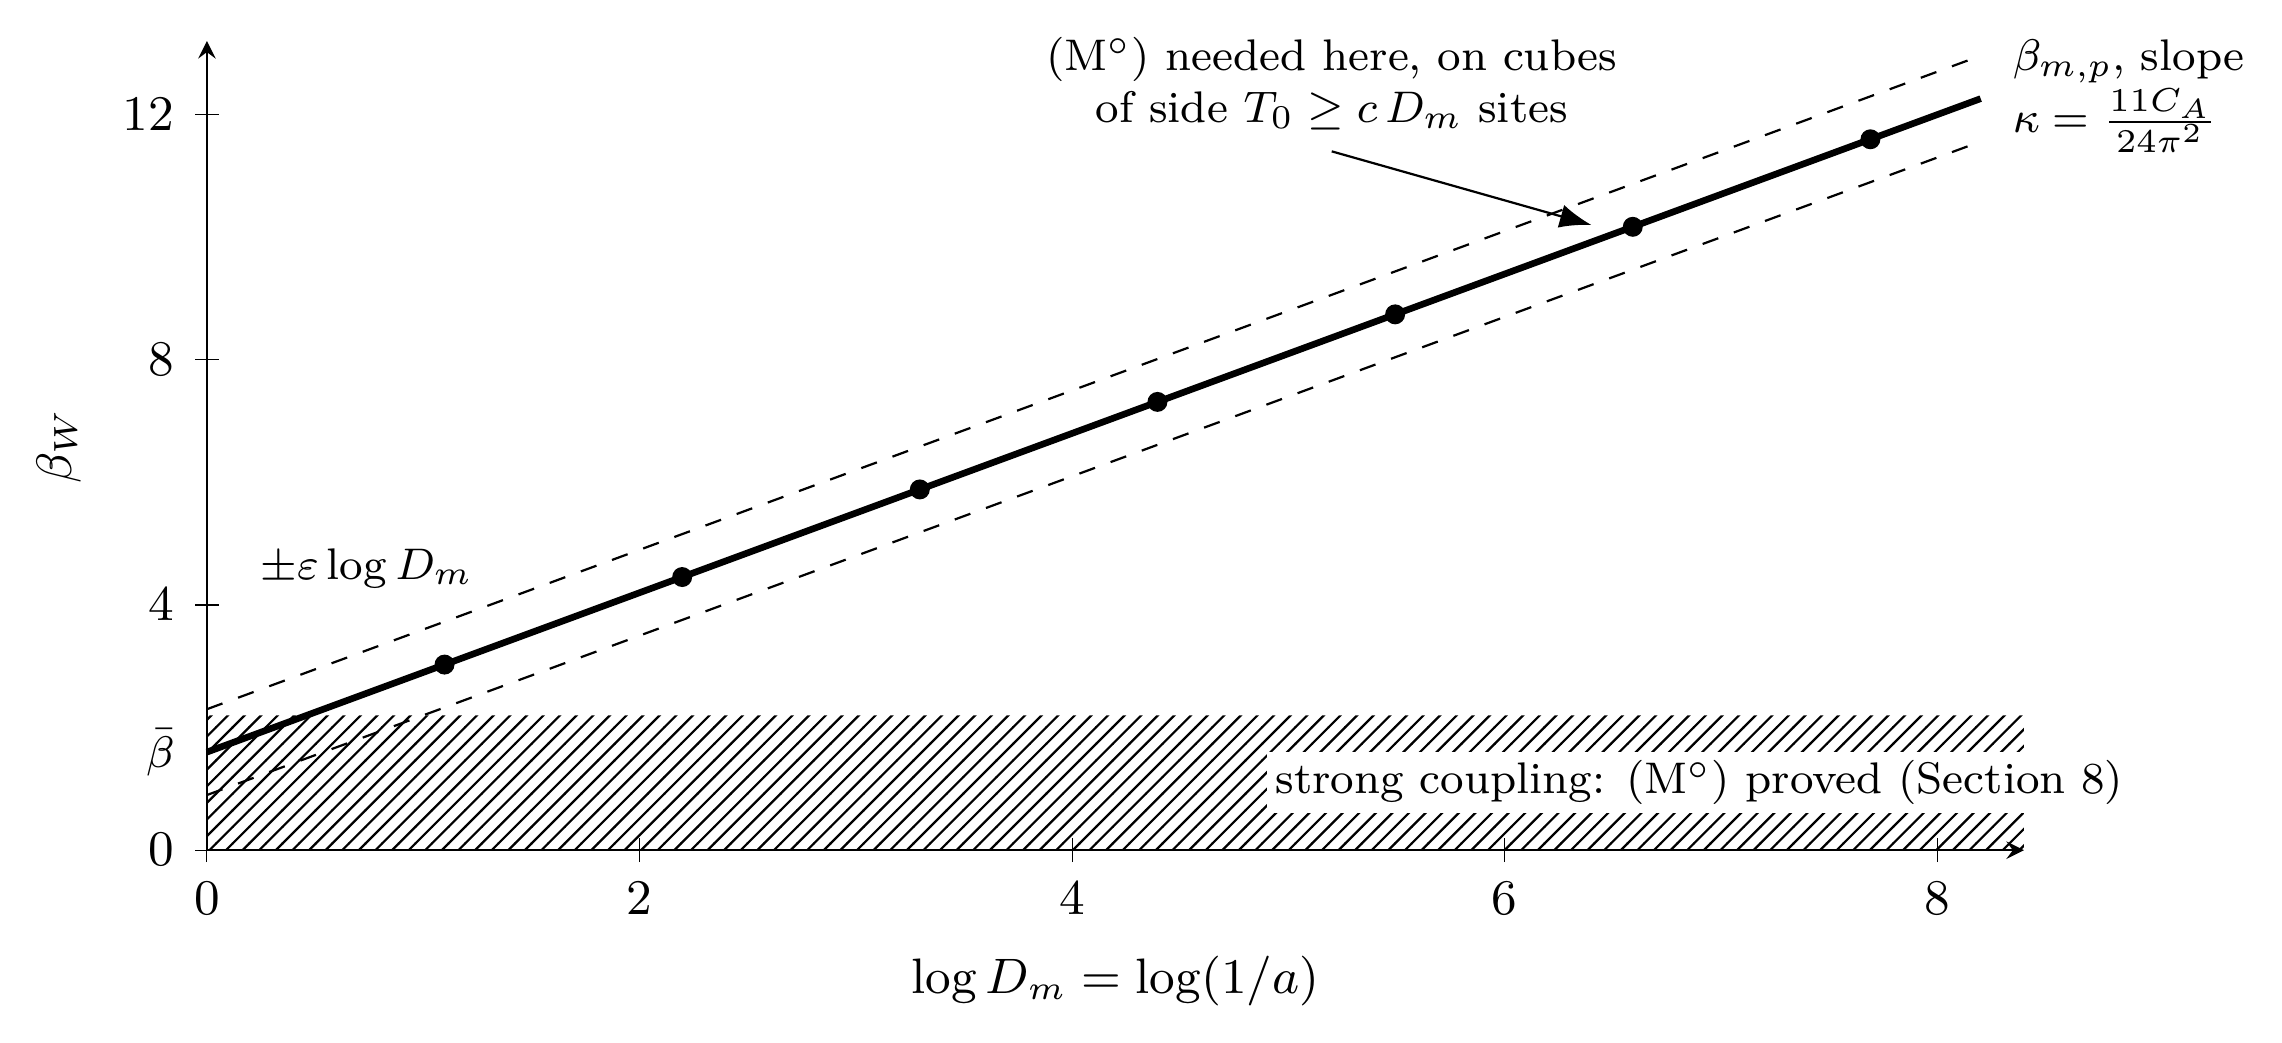
\includegraphics[width=410.6bp]{figures/fig04.png}
\caption{The tuning of the constructed family, drawn schematically. The coupling grows like $\kappa\log D_m$ with the asymptotic-freedom slope $\kappa=11C_A/(24\pi^2)$; the dots are the meshes $1/D_m$, the dashed lines the window $\pm\varepsilon\log D_m$ of the uniform limit. \Mcirc{} is proved only in the hatched strong-coupling strip; along the tuning it is needed on cubes whose side in lattice units grows at least in proportion to $D_m$ (\cref{prop:constructed-nontrivial}).}
\label{fig:tuning}
\end{figure}

The continuum limit (\texttt{Hierarchy.Properties}) consists of: functions $S^\chi_u$ and $S^\star_u$ on $D_n$, for $u$ an $n$-tuple of tokens and $\chi$ in a compact metric space $X$, smooth on $D_n$ (\texttt{smooth}); a Borel probability measure $\nu$ on $X$ of full support (\texttt{normalized}, \texttt{fullSupport}); continuity of $\chi\mapsto S^\chi_u(x)$ for every $x\in D_n$ (\texttt{characterContinuity}); the mixture identity
\begin{equation}\label{eq:oai-mixture}
S^\star_u(x)=\int_XS^\chi_u(x)\dd\nu(\chi)\qquad(x\in D_n)
\end{equation}
(\texttt{mixture}); the ordered limit (\texttt{Converges}): for every $n$, $u$ and test function $t\in C^\infty_c(D_n)$, along a strictly increasing sequence $(p_j)$,
\begin{equation}\label{eq:oai-limit}
\lim_{j\to\infty}\lim_{m\to\infty}S_{m,p_j}(u,t)=\int t\,S^\star_u ,
\end{equation}
where $S_{m,p}(u,t)$ is the lattice smear \eqref{eq:cont-smear} on the torus of side $P_pD_m$ with mesh $1/D_m$, the inner limit existing for every $p$ for which the support of $t$ lies in the box of side $P_p$; and, for one $\chi_*\in X$, a Wightman theory with a unique vacuum, generated by the fields of the tokens, whose Schwinger functions are the $S^{\chi_*}_u$ (\texttt{Reconstructed}, \texttt{root}). We write $S^\star$ for the unselected limit.

\begin{lemma}[the family as a continuum family]\label{lem:oai-family}
Put $\mathcal P=\{D_m:m\ge0\}$ and, for $N=D_m$, $\Lp=P_p$ and $\betaNp=\beta_{m,p}/N_c^2$. Let $V$ be the set of pairs $(w,\epsilon)$ with $w$ a token and $\epsilon\in\{0,1\}$, with $(w,\epsilon)^\vartheta=(w,1-\epsilon)$. For every $M\ge3$ and every site $x$ of $\Lambda_{N\Lp,M}$ let $\Phi^{N,p}_{(w,0)}(x,Q)$ be the polynomial of $\Phi^{m,p}_w$ evaluated on the links of $\Lambda_{N\Lp,M}$ obtained from the stencil around $x$ by reduction modulo the periods, and $\Phi^{N,p}_{(w,1)}(x,Q)=\overline{\Phi^{N,p}_{(w,0)}(\vartheta x,\vartheta Q)}$. Then:
\begin{enumerate}[label=(\alph*),leftmargin=2.2em]
\item these data form a continuum family over $\mathcal P$;
\item on the symmetric torus, $M=N\Lp$, $\Phi^{N,p}_{(w,0)}$ is the insertion of $w$ in \cite{openaiym}, and for $w=(d,v)$ and $m\ge r(d)$, $\Phi^{N,p}_{(w,1)}$ is the insertion of the token $w^\natural=(d,\overline{A_\vartheta v})$;
\item the convergence clause over $\mathcal P$ holds along the sequence $(p_j)$ of \eqref{eq:oai-limit}, and for a cluster $(u,t)$ the limit \eqref{eq:conv-clause} equals $\int t\,S^\star_{u'}$, where $u'$ replaces every $(w,0)$ by $w$ and every $(w,1)$ by $w^\natural$.
\end{enumerate}
\end{lemma}

\begin{proof}
(a) Continuity, gauge invariance and locality are inherited from the polynomial on the stencil; reduction modulo the periods maps a gauge transformation of $\Lambda_{N\Lp,M}$ to a gauge transformation of the stencil, under which the polynomial is invariant because it is invariant under all gauge transformations of a torus on which the stencil embeds. This gives (F1) with $R_{(w,\epsilon)}$ the stencil and its reflection. By (O1) the polynomial at $x$ is the polynomial at $0$ applied to $\tau_{-x}Q$, which is (F2) for $\epsilon=0$; for $\epsilon=1$, $\vartheta\tau_{-y}=\tau_{-\vartheta y}\vartheta$ on sites and configurations gives $\Phi_{(w,1)}(x+y,Q)=\overline{\Phi_{(w,0)}(\vartheta x,\tau_{-\vartheta y}\vartheta Q)}=\Phi_{(w,1)}(x,\tau_{-y}Q)$. (F3) holds by construction, since $\vartheta$ is an involution of sites and configurations. (b) The first claim is the definition. For the second, (O2) with $s=\vartheta$ and (O3) give $\Phi_{w^\natural}(\vartheta x,U)=\overline{\Phi_{(d,A_\vartheta v)}(\vartheta x,U)}=\overline{\Phi_w(x,\vartheta^*U)}$, and $\vartheta^*U$ is the configuration $\vartheta U$ of (F3), since the time-reversed temporal link from $\vartheta x$ is the link $(\vartheta x-e_0,0)$ traversed backwards. Replacing $x$ by $\vartheta x$ gives the claim. (c) For a cluster $(u,t)$ the smears $S_{N,p}(u,t)$ and $S_{m,p}(u',t)$ coincide once $m\ge r(d)$ for every token of $u$, by (b). Since $m\mapsto D_m$ is strictly increasing, the inner limit of \eqref{eq:oai-limit} along $m$ is a limit along $N\in\mathcal P$, and \eqref{eq:oai-limit} gives the rest.
\end{proof}

\begin{theorem}[the unselected limit]\label{thm:constructed-gap}
For the family of \cite{openaiym}, let \Mcirc{} hold along the tuning $\betaW=\beta_{m,p}$ with $\tzero>0$. Then the functional $S^\star(u,t)=\int t\,S^\star_{u'}$ of \cref{lem:oai-family}(c) satisfies the conclusions of \cref{thm:soft-limit}(a)--(e), and its Hamiltonian satisfies
\[
\sigma(H)\subset\{0\}\cup[\Delta,\infty),\qquad\ker H=\C\Omega,\qquad\Delta=\frac1\tzero\log\frac{63}{32} .
\]
\end{theorem}

\begin{proof}
By \cref{lem:oai-family} the family is a continuum family over $\mathcal P$ with the convergence clause over $\mathcal P$, and $S^\star$ is the functional $\bar S$ of \eqref{eq:conv-clause}. \Cref{prop:index-sets} and \cref{thm:main}(iii) give the claim.
\end{proof}

\subsection{The phases}
The second theorem needs every phase, not only the selected one, to be a Wightman theory \cite{wightman1956,streater2000}:
\begin{enumerate}[label=(R),leftmargin=3em]
\item for every $\chi\in X$ the functions $S^\chi_u$ are the Schwinger functions of a Wightman theory with a unique vacuum, generated by the fields of the tokens, in which the field of $w^\natural$ is the adjoint of the time-reflected field of $w$, in the sense of \cite[Section~7.5 and Lemma~13]{bhattacharjee2026first}.
\end{enumerate}
For $\chi=\chi_*$ this is part of the public statement of \cite{openaiym}. For every $\chi$ it is the reconstruction theorem for the component theories, \cite[Theorem~6.1]{ymgroup2026}, which lists vacuum uniqueness, adjoints and cyclicity among the proved properties of every phase (in the source, \texttt{constructed}, clause \texttt{view\_axioms}). The same assessment observes that clustering of the mixed limit would identify all the phases \cite[Section~6.2]{ymgroup2026}; \cref{thm:constructed-gap} supplies that clustering from \Mcirc, and the proof below carries out the identification pointwise.

\begin{theorem}[every phase]\label{thm:constructed-phases}
Under the hypotheses of \cref{thm:constructed-gap} and (R), $S^\chi_u=S^\star_u$ on $D_n$ for every $\chi\in X$ and every $u$, and the Hamiltonian of the Wightman theory of every phase, in particular of the selected phase $\chi_*$, has spectrum in $\{0\}\cup[\Delta,\infty)$ with $0$ a simple eigenvalue.
\end{theorem}

\begin{proof}
Fix an $n$-tuple $u$ of tokens of $V$ and a point $x\in D_n$ with all times positive. For $\sigma\ge0$ let $(\vartheta x,x+\sigma e_0)\in D_{2n}$ be the configuration with the points $\vartheta x_i$ carrying $u_i^\vartheta$ and the points $x_i+\sigma e_0$ carrying $u_i$, and put $k^\chi(\sigma)=S^\chi(\vartheta x,x+\sigma e_0)$ and $k^\star(\sigma)=S^\star(\vartheta x,x+\sigma e_0)$, the tokens being read through $u\mapsto u'$. The points are separated because the times of $\vartheta x$ are negative and those of $x+\sigma e_0$ positive. Let $f_k\ge0$ be smooth, supported in the ball of radius $1/k$ about $x$, with $\int f_k=1$, and let $A_k=(u,f_k)\in\mathcal A_+$ for large $k$.

\emph{Each phase.} By (R) and the Osterwalder--Schrader correspondence \cite{osterwalder1973} (\cite[Lemma~13]{bhattacharjee2026first}), the phase $\chi$ has a Hilbert space with vacuum $\Omega_\chi$, a Hamiltonian $H_\chi\ge0$ and vectors $[A]_\chi$ for $A\in\mathcal A_+$ with $S^\chi(A^\vartheta\tau_\sigma A)=\ip{[A]_\chi}{e^{-\sigma H_\chi}[A]_\chi}$ and $S^\chi(A)=\ip{\Omega_\chi}{[A]_\chi}$, where $S^\chi(A)$ is the smear of the $S^\chi_u$. By the spectral theorem $\sigma\mapsto S^\chi(A_k^\vartheta\tau_\sigma A_k)$ is nonincreasing and at least $\abs{S^\chi(A_k)}^2$. The test function of $A_k^\vartheta\tau_\sigma A_k$ concentrates at $(\vartheta x,x+\sigma e_0)$ and $S^\chi$ is continuous there, so letting $k\to\infty$: $k^\chi$ is nonincreasing on $[0,\infty)$ and $k^\chi(\sigma)\ge\abs{S^\chi_u(x)}^2\ge0$.

\emph{The unselected limit.} By \cref{thm:constructed-gap} and \eqref{eq:main-limit} with $B=A=A_k$ and $\sigma_1=1$, $\abs{S^\star(A_k^\vartheta\tau_\sigma A_k)-\abs{S^\star(A_k)}^2}\le e^{-\Delta(\sigma-1)}\bigl(S^\star(A_k^\vartheta\tau_1A_k)-\abs{S^\star(A_k)}^2\bigr)$ for integers $\sigma\ge1$. As $S^\star_{u'}$ is smooth on $D$, letting $k\to\infty$ gives $\abs{k^\star(\sigma)-\abs{S^\star_u(x)}^2}\le e^{-\Delta(\sigma-1)}k^\star(1)$, so $k^\star(\sigma)\to\abs{S^\star_u(x)}^2$.

\emph{Comparison.} By \eqref{eq:oai-mixture}, $k^\star(\sigma)=\int k^\chi(\sigma)\dd\nu$ and $S^\star_u(x)=\int S^\chi_u(x)\dd\nu$. The continuous function $\chi\mapsto k^\chi(0)$ on the compact space $X$ is bounded, and $0\le k^\chi(\sigma)\le k^\chi(0)$; by dominated convergence $\int\lim_\sigma k^\chi(\sigma)\dd\nu=\lim_\sigma k^\star(\sigma)=\abs{S^\star_u(x)}^2$. Hence
\[
\int_X\abs{S^\chi_u(x)}^2\dd\nu(\chi)\le\Bigl\lvert\int_XS^\chi_u(x)\dd\nu(\chi)\Bigr\rvert^2 ,
\]
and since $\nu$ is a probability measure, $\int\abs{S^\chi_u(x)-S^\star_u(x)}^2\dd\nu=\int\abs{S^\chi_u(x)}^2\dd\nu-\abs{S^\star_u(x)}^2\le0$. So $S^\chi_u(x)=S^\star_u(x)$ for $\nu$-almost every $\chi$. The set of $\chi$ where they differ is open, by continuity in $\chi$, and $\nu$-null, hence empty because $\nu$ has full support. Every $u$ in the sense of \cite{openaiym} is $u'$ for some $u\in V^n$, the functions $S^\chi_u$ are invariant under time translations by (R), and $S^\star_u$ by \cref{thm:soft-limit}(b) and continuity; translating in time gives $S^\chi_u=S^\star_u$ on all of $D_n$.

\emph{Spectrum.} The smears of $S^\chi$ and of $S^\star$ therefore agree on $\mathcal A$, so the reconstructions of \cref{thm:soft-limit}(e) coincide and \cref{thm:constructed-gap} applies to every phase. By the Osterwalder--Schrader correspondence for a Wightman theory generated by the fields of the tokens, the reconstructed Hilbert space and Hamiltonian are those of the Wightman theory of the phase.
\end{proof}

The gap given by \cref{thm:constructed-gap} is not that of a trivial theory, and the datum cannot hold at arbitrarily small physical scale along this tuning. Let $v_0$ be the label of the trace $\sum_\mu T_{\mu\mu}$ of the stress tensor of \cite[Section~7.1]{ymgroup2026}; it is fixed by field conjugation, $v_0^\natural=v_0$. For $r>0$ and $\chi\in X$ put $K^\chi(r)=S^\chi_{v_0v_0}(-\frac r2e_0,\frac r2e_0)$ and $s^\chi=S^\chi_{v_0}$, a constant by translation invariance, and define $K^\star$, $s^\star$ in the same way from $S^\star$.

\begin{proposition}[the gap is not vacuous]\label{prop:constructed-nontrivial}
Assume \textup{(R)}.
\begin{enumerate}[label=\textup{(\alph*)},leftmargin=*]
\item There is $r_0>0$ such that $K^\star(r)>\abs{s^\star}^2$ for $0<r<r_0$.
\item Let \Mcirc{} hold along the tuning with $\tzero$, and let $H$ be the Hamiltonian of \cref{thm:constructed-gap}. Then $\Omega^\perp\ne\{0\}$, $\Delta_\star=\inf\sigma(H|_{\Omega^\perp})$ is finite, and
\[
\tzero\ge\frac{1}{\Delta_\star}\log\frac{63}{32}.
\]
In particular \Mcirc{} does not hold along the tuning for every $\tzero>0$, and on the $m$-th lattice its cube has side $2T_0\ge2D_m\Delta_\star^{-1}\log\frac{63}{32}$ with $\log D_m=(\kappa^{-1}+o(1))\,\beta_{m,p}$, exponentially large in the Wilson coupling.
\end{enumerate}
\end{proposition}

\begin{proof}
(a) The step \emph{Each phase} of the proof of \cref{thm:constructed-phases}, applied to $u=(v_0)$ at $x=\frac r2e_0$ with $\sigma=0$, uses only (R) and gives $g(\chi)=K^\chi(r)-\abs{s^\chi}^2\ge0$ for every $\chi$. The function $g$ is continuous on $X$ (\texttt{characterContinuity}). In the selected phase the centred trace is $\Theta=v_0-s^{\chi_*}$, so that $S^{\chi_*}_{\Theta\Theta}(-\frac r2e_0,\frac r2e_0)=g(\chi_*)$, and by \cite[Theorem~7.1]{ymgroup2026}, $r^8\log^2(1/r)\,g(\chi_*)\to3\dim_\R\mathfrak g/\pi^4>0$ as $r\downarrow0$. Fix $r_0$ with $g(\chi_*)>0$ for $0<r<r_0$ and such an $r$. Then $g>g(\chi_*)/2$ on an open neighbourhood $U$ of $\chi_*$, and $\nu(U)>0$ because $\nu$ has full support, so $\int g\dd\nu>0$. By \eqref{eq:oai-mixture} and the Cauchy--Schwarz inequality $\abs{\int s^\chi\dd\nu}^2\le\int\abs{s^\chi}^2\dd\nu$,
\[
K^\star(r)-\abs{s^\star}^2=\int K^\chi(r)\dd\nu-\Bigl|\int s^\chi\dd\nu\Bigr|^2\ge\int g\dd\nu>0 .
\]
(b) Let $A_k=(v_0,f_k)$ with $f_k$ concentrating at $\frac r2e_0$ as in the proof of \cref{thm:constructed-phases}, and $[A_k]$ its vector in the Hilbert space of $S^\star$. If $\Omega^\perp=\{0\}$, then $\norm{[A_k]}^2=\abs{\ip{\Omega}{[A_k]}}^2$, that is $S^\star(A_k^\vartheta A_k)=\abs{S^\star(A_k)}^2$, and letting $k\to\infty$ gives $K^\star(r)=\abs{s^\star}^2$, against (a). So $\Omega^\perp\ne\{0\}$ and $\Delta_\star<\infty$. By \cref{thm:constructed-gap}, $\sigma(H|_{\Omega^\perp})\subset[\Delta,\infty)$ with $\Delta=\tzero^{-1}\log\frac{63}{32}$, so $\Delta_\star\ge\Delta$. The datum at physical scale $\tzero$ on the $m$-th lattice is the datum at $T_0=\lfloor\tzero D_m\rfloor$, and $\beta_{m,p}/\log D_m\to\kappa$.
\end{proof}

The same argument bounds every faster rate of decorrelation along the tuning. Write $\Zc_{N,p}$ as in \cref{thm:main}, at $N=D_m$ and the coupling $\beta_{m,p}$.

\begin{proposition}[no faster decorrelation]\label{prop:constructed-rate}
Assume \textup{(R)}, let $(p_j)$ be the sequence of \eqref{eq:oai-limit} and $\delta_{m,p}>0$, and suppose:
\begin{enumerate}[label=\textup{(\alph*)},leftmargin=*]
\item \emph{thermal control}: $\lim_{j\to\infty}\limsup_{m\to\infty}\bigl(\Zc_{D_m,p_j}-1\bigr)=0$;
\item \emph{gap}: for every large $j$ and $m$, every eigenvalue $\lambda\ne\lzero$ of the transfer matrix $\TT_{(D_mP_{p_j})^3}$ at $\beta_{m,p_j}$ satisfies $\lambda\le e^{-\delta_{m,p_j}}\lzero$.
\end{enumerate}
Then it is not true that $D_m\delta_{m,p_j}\to\infty$ as $m\to\infty$ for every large $j$. In particular, together with \textup{(a)}, neither a bound $\delta_{m,p}\ge c\,e^{-\beta_{m,p}/\kappa_1}$ with $\kappa_1>\kappa$ nor a bound $\delta_{m,p}\ge c\,\beta_{m,p}^{-k}$, with constants $c,k>0$, holds for all large $m$ and $p$.
\end{proposition}

\begin{proof}
Suppose that $D_m\delta_{m,p_j}\to\infty$ for every large $j$. Fix $A\in\mathcal A_+^{\delta,\omega}$ and an integer $\sigma\ge2$, and repeat the proof of \cref{thm:main}(iii) with $B=A$, $\sigma_1=1$, $N=D_m$ and $S=S^\star$ (\cref{lem:oai-family}(c)), with two changes. \Cref{lem:gap-decay}(b) is applied with $\gamma=\delta_{m,p_j}$, which (b) allows, so that the factor $e^{-\Delta(\sigma-1)}$ in \eqref{eq:main-decay} becomes $e^{-(\sigma-1)D_m\delta_{m,p_j}}$; and (a) replaces \cref{thm:main}(i) in the step from the torus to the cylinder, which still gives $\eta_j(C)\to0$. The factors under the root in \eqref{eq:main-decay} have limits superior over $m$ at most $\mathsf b+\eta'_j$ and $\mathsf c+\eta'_j$, so the limit superior over $m$ of the right side is $0$, and the passage to the limit gives $\abs{S^\star(A^\vartheta\tau_\sigma A)-\abs{S^\star(A)}^2}\le\eta'_j\to0$. Hence $S^\star(A^\vartheta\tau_\sigma A)=\abs{S^\star(A)}^2$.

Take $A_k=(v_0,f_k)$ with $f_k$ concentrating at $te_0$, $t>0$. As in the proof of \cref{prop:constructed-nontrivial}, letting $k\to\infty$ gives $K^\star(2t+\sigma)=\abs{s^\star}^2$, and the step \emph{Each phase} gives $g(\chi)=K^\chi(2t+\sigma)-\abs{s^\chi}^2\ge0$. By \eqref{eq:oai-mixture} and the Cauchy--Schwarz inequality, $\int g\dd\nu=K^\star(2t+\sigma)-\int\abs{s^\chi}^2\dd\nu\le K^\star(2t+\sigma)-\abs{s^\star}^2=0$, so $g=0$ $\nu$-almost everywhere, and everywhere because $g$ is continuous and $\nu$ has full support. For $\chi=\chi_*$ this says that $r\mapsto S^{\chi_*}_{\Theta\Theta}(-\frac r2e_0,\frac r2e_0)$ vanishes for every $r>2$. The Schwinger functions of a Wightman theory are real-analytic at noncoinciding points, as restrictions of the analytic continuations of its Wightman functions \cite{osterwalder1973}, so this function vanishes for every $r>0$, against \cite[Theorem~7.1]{ymgroup2026}.

For the rates, $\beta_{m,p}/\log D_m\to\kappa$ uniformly in $p$ gives $\beta_{m,p}\le(\kappa+\varepsilon)\log D_m$ for large $m$ and every $p$. With $0<\varepsilon<\kappa_1-\kappa$ this yields $D_m e^{-\beta_{m,p}/\kappa_1}\ge D_m^{1-(\kappa+\varepsilon)/\kappa_1}\to\infty$, and $D_m\beta_{m,p}^{-k}\ge D_m\bigl((\kappa+\varepsilon)\log D_m\bigr)^{-k}\to\infty$.
\end{proof}

Under \Mcirc{}, \cref{thm:main}(i),(ii) give (a) and (b) with $\delta_{m,p}=\Delta/D_m$, so $D_m\delta_{m,p}=\Delta$ stays bounded: \Mcirc{} sits exactly at the borderline rate allowed by \cref{prop:constructed-rate}, and no lattice gap estimate that is uniform in the volume and decays more slowly than $1/D_m$ can be combined with thermal control along this tuning.

By \cref{prop:constructed-nontrivial}, \Mcirc{} along this tuning would give the gap of a theory whose stress-trace two-point function does not factorise, and the side of its cube must grow, in lattice units, at least in proportion to $D_m$.

The tuning of \cite{openaiym} has $\betaW\sim\kappa\log(1/\aN)\to\infty$, so \Mcirc{} along it is a weak-coupling statement; the strong-coupling ranges of \cref{sec:ranges} do not reach it. Granted the statements of \cite{openaiym,ymgroup2026}, \cref{thm:constructed-phases} reduces the four-dimensional mass gap for every compact connected simple gauge group to \Mcirc{} along this single tuning. \Mcirc{} along this tuning is not proved. The nontriviality test of \cite{openaiym} is a short-distance coefficient $3\dim_\R\mathfrak g/\pi^4$ of the two-point function of the trace of the stress tensor together with the exclusion of finite sums of mass-shell kernels, which by \cite{ymgroup2026} does not exclude every description by composites of Gaussian fields; by \cref{ms:prop:GFF} a positive local field with the same coefficient and continuous spectral weight down to zero has no gap, so the test does not by itself bear on the gap.

\emph{Connectedness.} The class of \cite{openaiym} contains disconnected groups. For a closed $G_0\subset\U(m_0)$ with simple Lie algebra and $k\ge1$, the group $G'=\{\operatorname{diag}(g,h\mathbf 1_k):g\in G_0,\ h=\pm1\}\subset\U(m_0+k)$ is isomorphic to $G_0\times\{\pm1\}$ and has the Lie algebra of $G_0$. Since $\ReTr\operatorname{diag}(g,h\mathbf 1_k)=\ReTr g+kh$ and the Haar measure of $G'$ is the product of the Haar measures of the factors, the Wilson measure of $G'$ at coupling $\betaW$ is, on every torus, the product of the Wilson measure of $G_0$ at coupling $\betaW m_0/(m_0+k)$ and the $\Z/2$ measure with weight $\exp\bigl(\frac{\betaW k}{m_0+k}\sum_ph_p\bigr)$. Logarithms of partition functions, and so $\psiT{\cube{T_0}}{T_0}=2\XT{\cube{T_0}}{T_0}-\XT{\cube{T_0}}{2T_0}$, are therefore sums of the two contributions, while insertions supported on the $G_0$ block have the same moments as for $G_0$. The $G_0$ contribution is nonnegative, since $\Tr R^{2T}\le(\Tr R^T)^2$, and the $\Z/2$ contribution exceeds $2.07$ on every cube $\cube{T_0}\times T_0$, $T_0\ge3$, once $\beta'=\betaW k/(m_0+k)\ge4$ (\cref{lem:z2-violation} below). So \Mcirc{} fails along every tuning of $G'$ with $\betaW\to\infty$. Hence \Mcirc{} is not determined by the continuum correlators of the tokens alone: a proof of it must use that $G$ is connected, and \cref{thm:constructed-gap,thm:constructed-phases} have content only for connected $G$.

\begin{figure}[htbp]
\centering
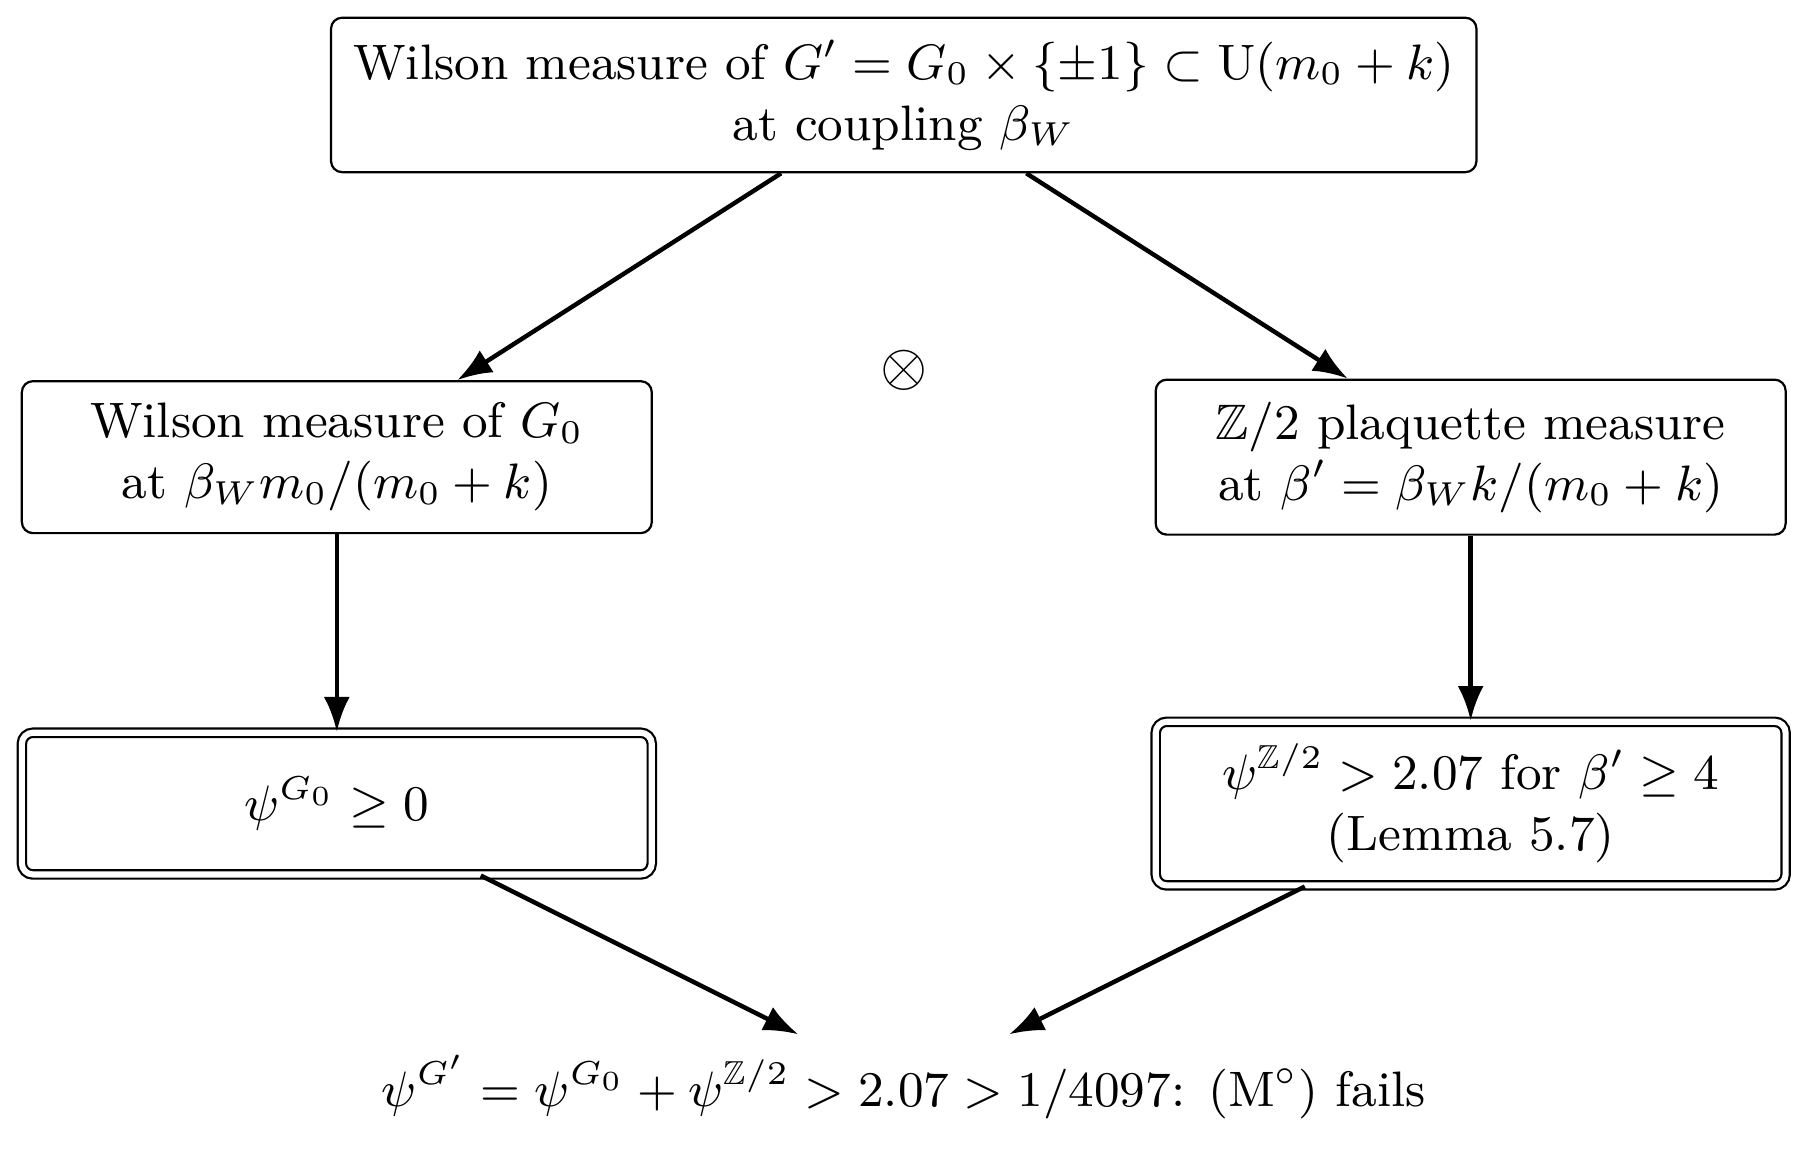
\includegraphics[width=325.4bp]{figures/fig05.png}
\caption{Why a proof of \Mcirc{} must use connectedness. The Wilson measure of $G_0\times\{\pm1\}$ factorises, the logarithms of partition functions add, and the $\Z/2$ factor alone violates \Mcirc{} on every cube once $\beta'\ge4$.}
\label{fig:factor}
\end{figure}

\begin{lemma}\label{lem:z2-violation}
For the $\Z/2$ gauge theory with weight $\exp(\beta'\sum_ph_p)$, $\beta'\ge4$, and every integer $T\ge3$, the torus $\cube T\times T$ has $\XT{\cube T}{T}\ge\log8-7\Gamma>2.07$ and $\psiT{\cube T}{T}\ge\XT{\cube T}{T}$, where $\Gamma\le48T^4e^{-2\beta'}q^{2T^2-1}/(1-q)\le2.3\cdot10^{-15}$ and $q=400e^{-2\beta'}$.
\end{lemma}

\begin{proof}
Write $\Z/2$ additively and, for a $2$-cochain $\eta$, let $Z(\eta)$ be the partition function with every plaquette variable multiplied by $(-1)^{\eta_p}$. The map $\sigma\mapsto d\sigma+\eta$ from $1$-cochains is $\abs{\ker d}$-to-one onto $\eta+\operatorname{im}d$, and $\sum_p(-1)^{e_p}=\abs P-2\abs e$, so for a cocycle $\eta$, $Z(\eta)=e^{\beta'\abs P}\abs{\ker d}\,\Phi([\eta])$ with $\Phi(c)=\sum_{e\in c}e^{-2\beta'\abs e}$, a function of the class $c\in H^2(\Lambda;\Z/2)\cong(\Z/2)^6$. Its basis is given by the stacks $S_{\mu\nu}$ of $(\mu,\nu)$-plaquettes with $x_\mu=L_\mu-1$, $x_\nu=L_\nu-1$, which pair with the coordinate $2$-tori $\Pi_{\rho\sigma}(y)$ as $\delta_{\{\mu\nu\},\{\rho\sigma\}}$.

\emph{Step 1: $\Phi(c)\le\Phi(0)$.} With time in direction $\tau$, a stack $S_{j\tau}$ inserts into the transfer matrix the flip $z_j$ of all $j$-links on the hyperplane $x_j=L_j-1$, while the stacks $S_{ij}$, $i,j\ne\tau$, change the signs of spatial plaquettes in every slice. The flips commute with the gauge projection and with the twisted transfer matrix $A\ge0$ of the spatial stacks, so $\abs{\Tr(z^cA^{L_\tau})}\le\Tr A^{L_\tau}$ and $Z(\eta)\le Z(\eta_{\mathrm{sp}})$, where $\eta_{\mathrm{sp}}$ keeps the spatial stacks. Applying this with $\tau=4,3,2$ in turn removes all six stacks.

\emph{Step 2: a nontrivial class costs area.} Call two plaquettes adjacent when they are faces of a common $3$-cube; each plaquette has at most $20$ neighbours. The adjacency components of a cocycle are cocycles, since the faces of one $3$-cube in $e$ are pairwise adjacent. If $c\ne0$, every $e\in c$ has a component $C$ with $[C]\ne0$, and choosing the first such $C$ in a fixed order makes $e\mapsto(C,e\setminus C)$ injective, so by Step~1 $\Phi(c)\le\Gamma\Phi(0)$ with $\Gamma=\sum e^{-2\beta'\abs C}$ over connected cocycles with $[C]\ne0$. Such a $C$ meets every one of the disjoint tori $\Pi_{\mu\nu}(y)$ for some $\mu<\nu$, so $\abs C\ge2T^2$ on $\cube T\times T$. A connected set of $n$ plaquettes through a given one is the vertex set of a closed walk of $2(n-1)$ steps along a spanning tree, so there are at most $20^{2(n-1)}$ of them\footnote{A spanning tree of the connected set, traversed once in each direction, is a closed walk of $2(n-1)$ steps on a graph of degree at most $20$, and it determines the set.}, and with $48T^4$ plaquettes $\Gamma\le48T^4e^{-2\beta'}q^{2T^2-1}/(1-q)$, which is decreasing in $\beta'$ and in $T\ge3$ and at most $2.3\cdot10^{-15}$ at $\beta'=4$, $T=3$.

\emph{Step 3.} With time in direction $4$ let $P_0$ be the average of the eight flips $z^k$. Then $w_0=\Tr(P_0R^T)/\Tr R^T=\frac18\sum_kZ(k)/Z(0)\le(1+7\Gamma)/8$, where $Z(k)$ carries the twist $\sum_jk_jS_{j4}$. The transfer matrix has positive entries in the configuration basis, so its Perron vector $\Omega$ is fixed by the gauge transformations and by the flips, and $\Tr(P_0R^T)\ge\ip{\Omega}{R^T\Omega}=1$. Hence $\Zc=\Tr R^T\ge1/w_0$ and $X\ge\log8-\log(1+7\Gamma)\ge\log8-7\Gamma>2.07$, since $\log8>2.075$. Finally $\Tr R^{2T}\le\Tr R^T$ because the spectrum of $R$ lies in $[0,1]$, so $\psi=2X(T)-X(2T)\ge X(T)$.
\end{proof}

\begin{figure}[htbp]
\centering
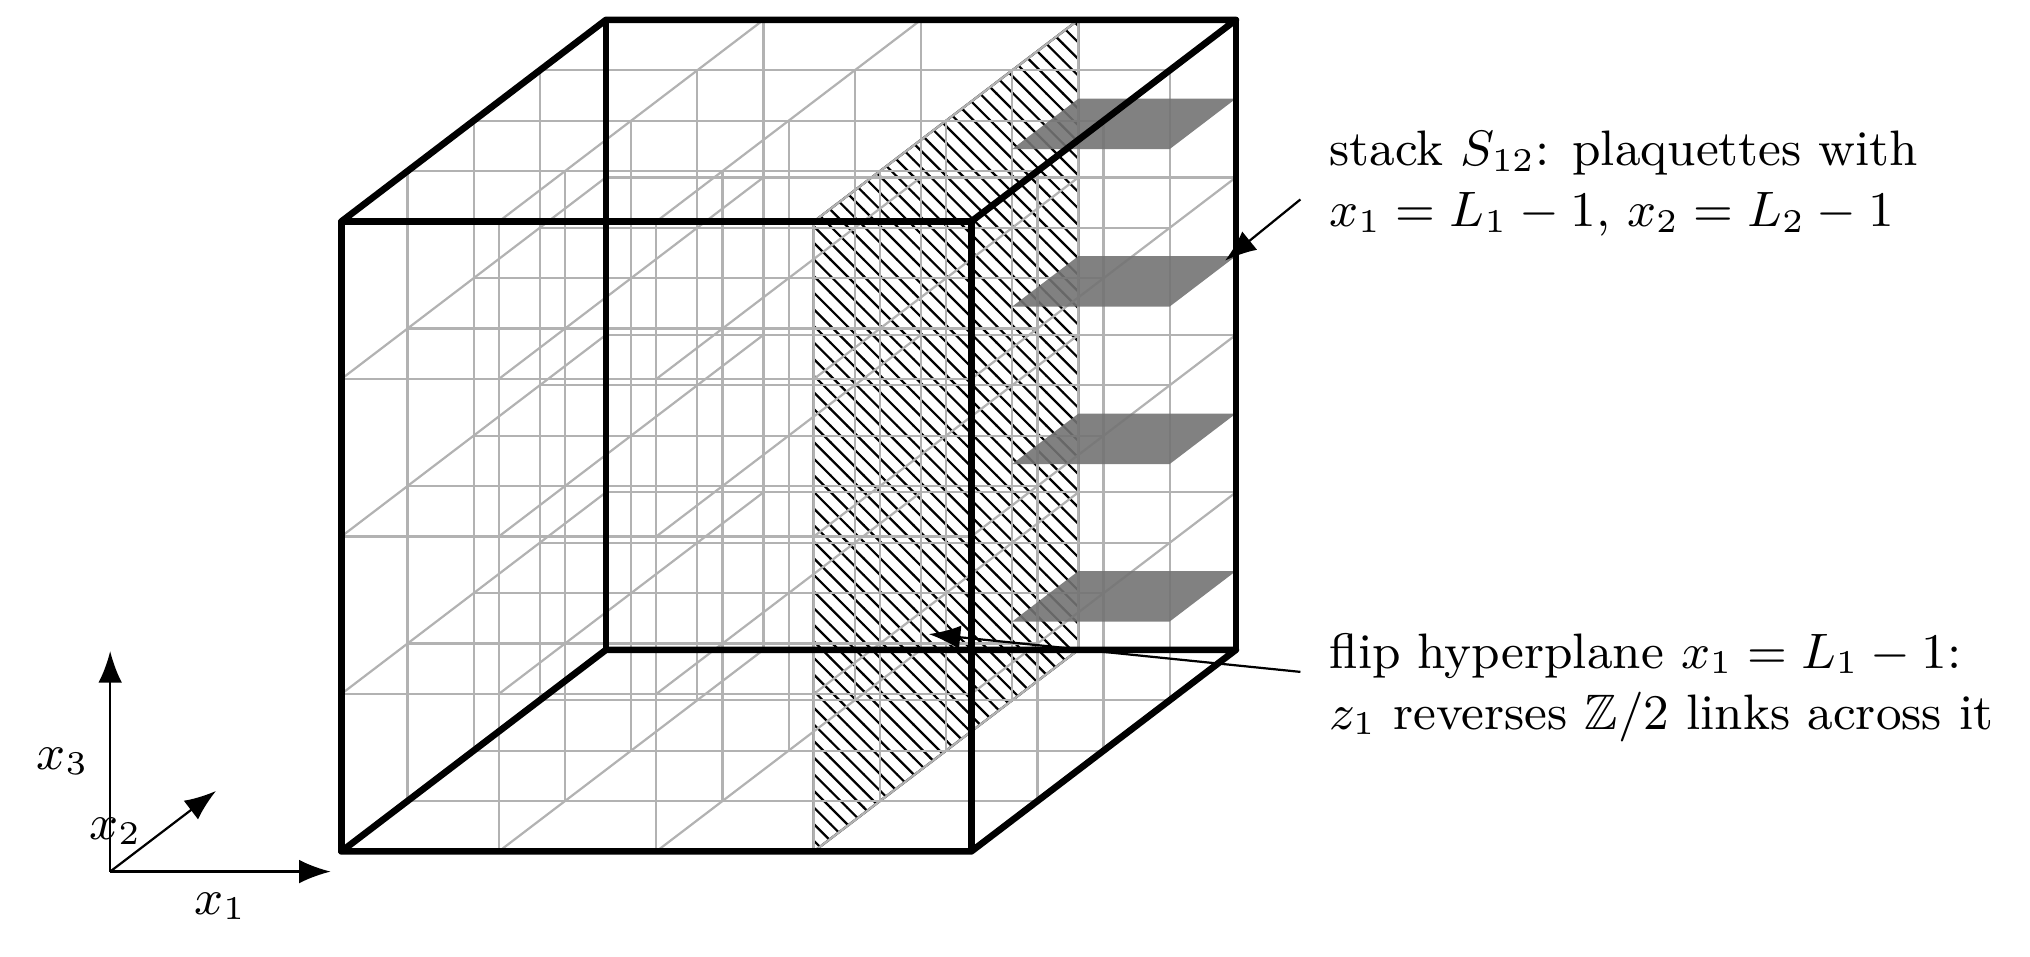
\includegraphics[width=365.4bp]{figures/fig06.png}
\caption{The objects in the proof of \cref{lem:z2-violation}, on a spatial slice of the torus: one stack $S_{12}$ of plaquettes (shaded) whose $\Z/2$ flux carries the nontrivial cohomology class, and one flip hyperplane (hatched), across which the flip $z_1$ reverses the signs of the links.}
\label{fig:stacks}
\end{figure}

\subsection{A step-scaling deduction}
The strong-coupling datum of \cref{sec:ranges} holds on cubes of fixed size at couplings $\betaW\le1/5$ ($\SU(2)$) or $\betaW\le1/20$ (every compact $G$). The datum along a tuning would follow if the defect could be carried up the tuning by one joint move, the lattice scale multiplied by $b$ and the coupling raised by $\kappa\log b$.\footnote{This is the lattice form of a step-scaling function: the same physical box is compared at two lattice spacings whose couplings differ by the one-loop shift. Nonperturbative step-scaling functions of this kind are the standard tool of lattice computations of the running coupling, where they are measured, not proved.} The next three statements make this precise, show that the move cannot start at coupling $0$, and show that it is tied to the asymptotic-freedom slope and to connectedness of $G$.

\begin{proposition}[strict positivity of the defect]\label{prop:psi-positive}
Let $G\subset\U(d)$ be compact, $G\ne\{1\}$, $s$ a spatial torus with all sides at least $3$ and $T\ge1$. Then $\psiT sT=0$ at $\betaW=0$ and $\psiT sT>0$ for every $\betaW>0$.
\end{proposition}

\begin{proof}
By \cref{lem:transfer-matrix}(i), $\Zpart sM=\Tr\TT_s^M$ with $\TT_s=D\Pi K\Pi D$, $D$ multiplication by a strictly positive gauge-invariant function, $\Pi$ the gauge projection and $K$ the product over spatial links of kernels $\exp(c\ReTr UV^*)$, $c>0$ proportional to $\betaW$. Expanding the exponential, $\ip f{Kf}=\sum_kc^kQ_k(f)/k!$ with every $Q_k(f)\ge0$, since each $(\ReTr UV^*)^k$ is a sum of kernels $\phi(U)\overline{\phi(V)}$ over monomials in the entries; $\ip f{Kf}=0$ forces $f$ to be orthogonal to every polynomial in the entries and their conjugates, hence $f=0$ by the Stone--Weierstrass theorem. So $\ip f{\TT_sf}=\ip{Df}{K\,Df}>0$ for $0\ne f\in\operatorname{Ran}\Pi$. The range of $\Pi$ contains the constants and $U\mapsto\ReTr Q_p(U)$ for a spatial plaquette $p$, which is not constant: $\ReTr g=d$ only for $g=1$, and $Q_p=g\ne1$ when $g$ sits on one link of $p$. So $\TT_s$ has at least two positive eigenvalues $\lzero\ge\lambda_1\ge\dots>0$ on $\operatorname{Ran}\Pi$. With $r_i=\lambda_i/\lzero$ and $a=\sum_{i\ge1}r_i^T>0$, $\Zs sT=1+a$ and $\Zs s{2T}=1+\sum_{i\ge1}r_i^{2T}\le1+a^2$, so $\psiT sT\ge\log\bigl((1+a)^2/(1+a^2)\bigr)>0$. At $\betaW=0$, $K$ is a multiple of the projection onto functions constant in the temporal links, $\TT_s$ has one nonzero eigenvalue on $\operatorname{Ran}\Pi$ and $\psiT sT=0$.
\end{proof}

For $\kappa>0$, $0<\beta_1<\beta_2$ and an integer $T_1\ge3$, let $\mathrm{MON}_\kappa[\beta_1,\beta_2;T_1]$ be the statement: for every $\beta\in[\beta_1,\beta_2]$ and every odd $b\ge3$,\footnote{Odd factors are those by which the lattices of \cite{openaiym} are blocked: their meshes are $1/D_m$ with $D_m=\prod_{k<m}b_k$ and odd $b_k\ge3$.}
\begin{equation}\label{eq:MON}
\psiT{\cube{bT_1}}{bT_1}\Big|_{\betaW=\beta+\kappa\log b}\le\psiT{\cube{T_1}}{T_1}\Big|_{\betaW=\beta} .
\end{equation}
By \cref{prop:psi-positive} and continuity of $\psi$ in $\betaW$ on a finite torus, \eqref{eq:MON} fails for seeds $\beta$ close to $0$, so $\beta_1>0$ is necessary: the move compares a nonzero strong-coupling defect with a weak-coupling one, and is not a monotonicity in $\betaW$.

\begin{proposition}[step scaling gives the datum]\label{prop:step-scaling}
Let $G=\SU(2)$, $0<\beta_1<1/5$, $\kappa>0$, and assume $\mathrm{MON}_\kappa[\beta_1,1/5;342]$. Let a tuning satisfy $\beta_{N,p}\to\infty$ and $\beta_{N,p}\le\kappa\log N+C$ for all large $N$, uniformly in $p$. Then \Mcirc{} holds along the tuning with
\[
\tzero=342\,e^{(C-\beta_1)/\kappa} .
\]
The same holds for every compact $G$ with $1/5$ replaced by $1/20$ and $342$ by $316$.
\end{proposition}

\begin{proof}
Fix $0<\delta\le1/5-\beta_1$ and put $x=e^{(\betaNp-\beta_1)/\kappa}$; for large $N$, $x(1-e^{-\delta/\kappa})\ge4$. Let $q$ be the largest odd integer at most $x$. Then $q\ge x-2\ge xe^{-\delta/\kappa}+2$, so $q\ge3$ and $xe^{-\delta/\kappa}\le q\le x$, and $\beta'=\betaNp-\kappa\log q$ satisfies $\beta_1\le\beta'\le\beta_1+\delta\le1/5$. By \cref{cor:certified-triples}(a) and the $\SU(2)$ triple $(1/5,23/20,342)$ of \cref{tab:certified-triples}, $\psi_{(2\cdot342)^3}(342)\le1/2225664$ at coupling $\beta'$. \eqref{eq:MON} with $\beta=\beta'$ and $b=q$ gives $\psi_{(2\cdot342q)^3}(342q)\le1/2225664<\dconstinl$ at coupling $\beta'+\kappa\log q=\betaNp$, that is \Mcirc{} at $\Tzero=342q$, and $3\le\Tzero\le342x\le342\,e^{(C-\beta_1)/\kappa}N$. For general $G$ use the triple $(1/20,7/6,316)$.
\end{proof}

\begin{figure}[htbp]
\centering
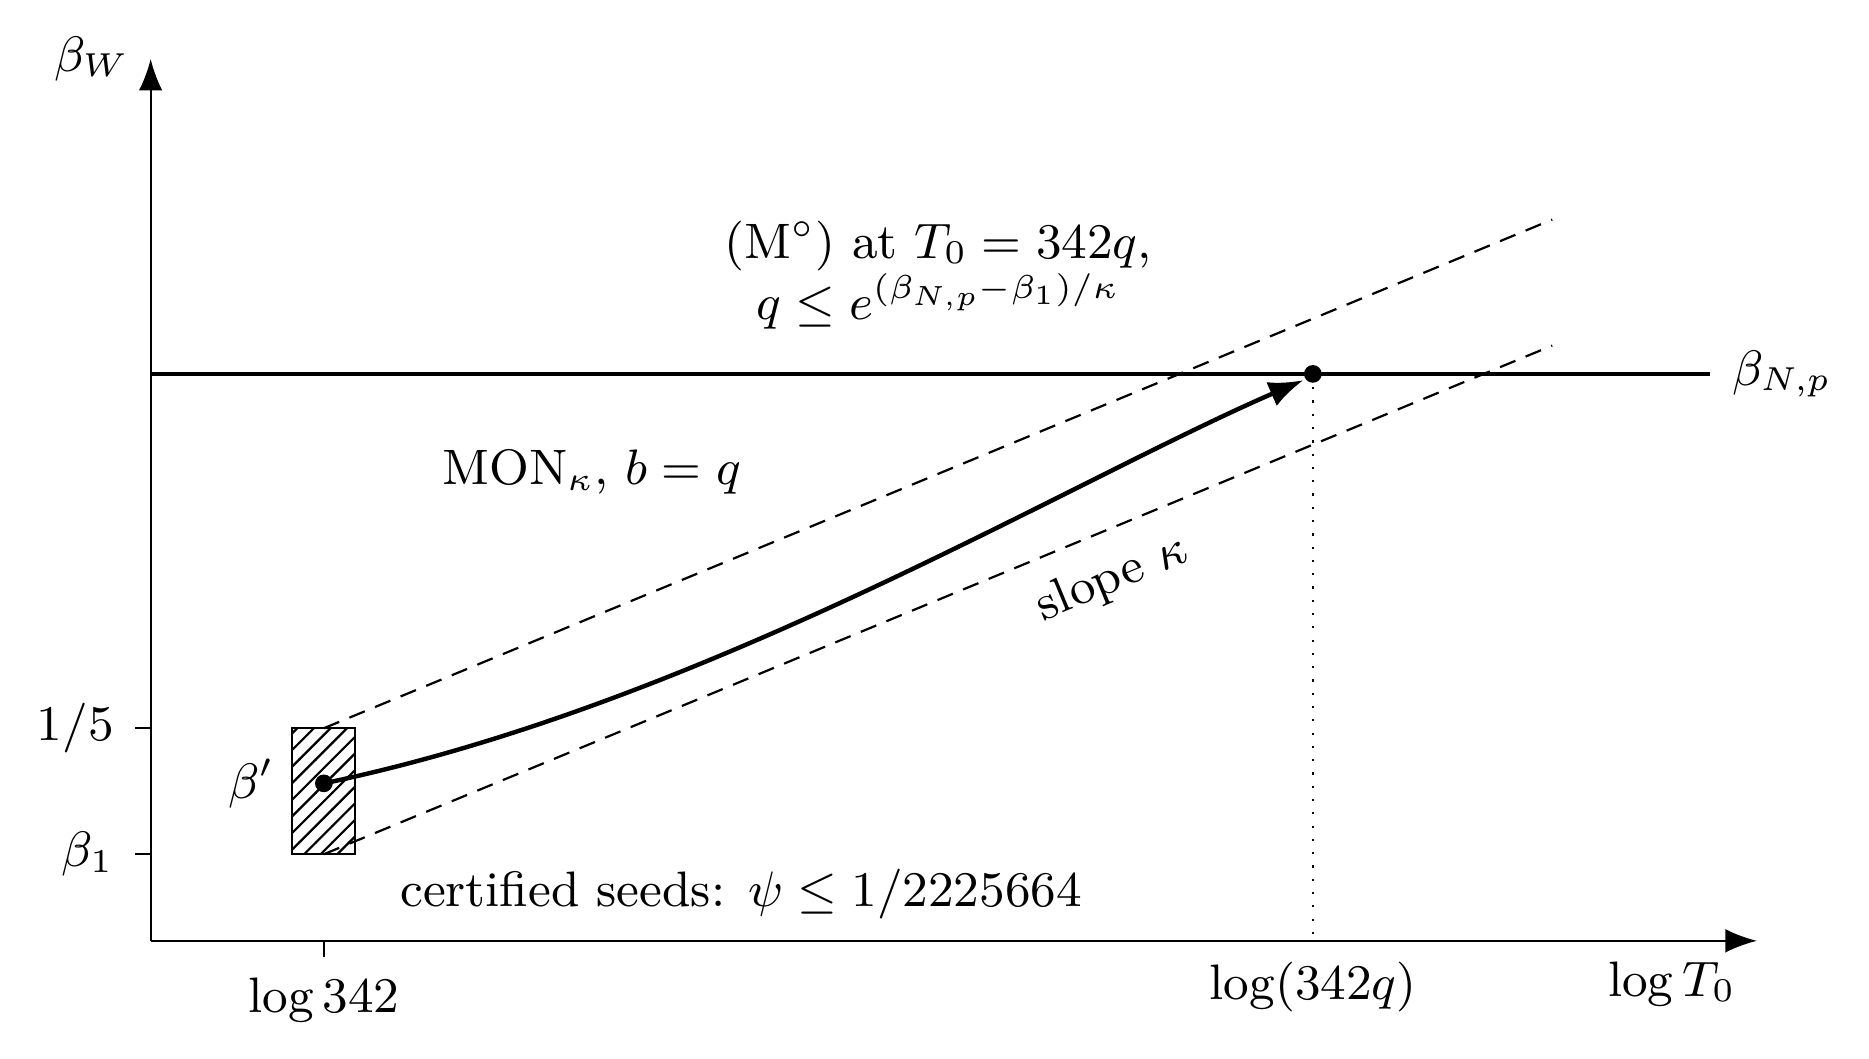
\includegraphics[width=336.2bp]{figures/fig07.png}
\caption{The move of \cref{prop:step-scaling}, schematically. A certified seed at coupling $\beta'\in[\beta_1,1/5]$ on the cube of side $342$ is carried by one application of $\mathrm{MON}_\kappa$ with $b=q$ to the cube of side $342q$ at coupling $\beta'+\kappa\log q=\betaNp$. The odd integer $q$ is chosen so that the line of slope $\kappa$ through the seed band meets the tuning coupling.}
\label{fig:staircase}
\end{figure}

At $\kappa=\kappa_{\mathrm{AF}}=11C_A/(24\pi^2)$ the rate is linear in $N$, the borderline rate of \cref{prop:constructed-rate}. For the family of \cite{openaiym}, $\beta_{m,p}/\log D_m\to\kappa$ uniformly in $p$ gives, from $\mathrm{MON}_\kappa$ and the same proof, the datum at some $\Tzero\le C_\varepsilon D_m^{1+\varepsilon}$ for every $\varepsilon>0$; the linear rate needs in addition $\beta_{m,p}\le\kappa\log D_m+C$, which holds if the per-step drifts of its renormalisation history are summable; the development does not establish this.\footnote{In \cite{openaiym} the coupling after $m$ block steps from the unit scale differs from $\bar\beta+\kappa\log D_m$ by the sum of the per-step drifts $\delta_k=\beta_{k+1}-\beta_k-\kappa\log b_k$, and $\abs{\delta_k}\le\log b_k/J(k+1)^2$ (\texttt{Transfer}, \texttt{Fits.driftSmall}). This bound is not summable: \texttt{Fits.logCost}, with \texttt{columns\_ge}, forces $\log b_k>J(k+1)^2\log2$, so each bound exceeds $\log2$, and the block factors $b_k$ are nondecreasing and unbounded (\texttt{sameFactor}, \texttt{monotoneL}, \texttt{deep}), with $\log b_k/\log D_k\to0$ (\texttt{Gentle}). The statements of the development give $\sum_{k<m}\delta_k=o(\log D_m)$ (\texttt{Running}) and are consistent with bounded and with unbounded drift. Two-loop running at fixed unit-scale coupling predicts $\sum_{k<m}\delta_k=\frac{51}{121}\kappa\log\log D_m+O(1)$, which is unbounded; see \cref{rem:step-general}(ii).} The slope cannot be taken larger, and the group cannot be disconnected:

\begin{proposition}[rigidity of the step]\label{prop:step-rigidity}
\begin{enumerate}[label=\textup{(\alph*)},leftmargin=*]
\item Let $G=\SU(N_c)$ and assume \textup{(R)}. For every $\kappa'>\kappa_{\mathrm{AF}}$ and every seed interval $[\beta_1,\beta_2]\subset(0,1/20]$, $\mathrm{MON}_{\kappa'}[\beta_1,\beta_2;316]$ is false.
\item Let $G'=G_0\times\{\pm1\}\subset\U(m_0+k)$ with $G_0\ne\{1\}$, as in the paragraph on connectedness. For every $\kappa>0$, every $[\beta_1,\beta_2]\subset(0,1/20]$ and every $T_1\ge316$, $\mathrm{MON}_\kappa[\beta_1,\beta_2;T_1]$ is false for $G'$.
\end{enumerate}
\end{proposition}

\begin{proof}
(a) Choose $\varepsilon'>0$ with $\kappa_{\mathrm{AF}}+\varepsilon'<\kappa'$. For large $m$, $(\kappa_{\mathrm{AF}}-\varepsilon')\log D_m\le\beta_{m,p}\le(\kappa_{\mathrm{AF}}+\varepsilon')\log D_m$ uniformly in $p$, and the proof of \cref{prop:step-scaling} with $\kappa'$ in place of $\kappa$ gives \Mcirc{} at some $\Tzero\le316\,e^{-\beta_1/\kappa'}D_m^{(\kappa_{\mathrm{AF}}+\varepsilon')/\kappa'}$. The exponent is less than $1$, so \Mcirc{} holds along the tuning for every $\tzero>0$, against \cref{prop:constructed-nontrivial}(b).
(b) By the factorisation in the paragraph on connectedness, $\psi^{G'}=\psi^{G_0}+\psi^{\Z/2}$ with both terms nonnegative (\cref{prop:psi-positive}). At every seed the right side of \eqref{eq:MON} is at most $1/2225664$ by \cref{cor:certified-triples}, which applies to every compact group. For odd $b$ so large that $(\beta_1+\kappa\log b)k/(m_0+k)\ge4$, \cref{lem:z2-violation} makes the left side larger than $2.07$.
\end{proof}

\begin{remark}[other steps, the drift, and the reach of the seeds]\label{rem:step-general}
(i) The proof of \cref{prop:step-scaling} uses only that $h(b)=\kappa\log b$ is continuous, strictly increasing and unbounded with $h(b+2)-h(b)\to0$. For every such $h$, let $\mathrm{MON}^h$ be \eqref{eq:MON} with $\kappa\log b$ replaced by $h(b)$. Then $\mathrm{MON}^h[\beta_1,1/5;342]$ and a tuning with $\betaNp\to\infty$ and $\betaNp\le\beta_1+h(tN)$ for large $N$, uniformly in $p$, give \Mcirc{} with $\tzero=342\,t$: take for $q$ the largest odd integer with $h(q)\le\betaNp-\beta_1$, so that $\beta'=\betaNp-h(q)$ lies in $[\beta_1,\beta_1+h(q+2)-h(q)]$, which is contained in $[\beta_1,1/5]$ for large $N$ because $q\to\infty$, and $q\le tN$ because $h$ is increasing. For the two-loop step $h_2(b)=\kappa_{\mathrm{AF}}\log b+\frac{51}{121}\kappa_{\mathrm{AF}}\log\log b$ (the ratio $b_1/(2b_0^2)=51/121$ of the first two coefficients of the beta function is the same for every simple gauge group) this covers tunings with $\betaNp\le\kappa_{\mathrm{AF}}\log N+\frac{51}{121}\kappa_{\mathrm{AF}}\log\log N+C$, and the proof of \cref{prop:step-rigidity}(a) excludes every $h$ with $h(b)\ge\kappa'\log b$ for large $b$ and some $\kappa'>\kappa_{\mathrm{AF}}$.

(ii) Let $G=\SU(N_c)$, assume \textup{(R)}, let \Mcirc{} hold along the tuning of \cite{openaiym} and suppose its drift is bounded, $\beta_{m,p}\le\kappa_{\mathrm{AF}}\log D_m+C$. Then there are no $c,k>0$ such that, for all large $m$ and $p$, every eigenvalue $\lambda\ne\lzero$ of $\TT_{(D_mP_p)^3}$ at $\beta_{m,p}$ satisfies $\lambda\le\exp(-c\,\beta_{m,p}^ke^{-\beta_{m,p}/\kappa_{\mathrm{AF}}})\lzero$. Indeed \Mcirc{} gives hypothesis (a) of \cref{prop:constructed-rate}, the eigenvalue bound gives (b) with $\delta_{m,p}=c\,\beta_{m,p}^ke^{-\beta_{m,p}/\kappa_{\mathrm{AF}}}$, and $D_m\delta_{m,p}\ge c\,e^{-C/\kappa_{\mathrm{AF}}}\beta_{m,p}^k\to\infty$. Two-loop scaling predicts lattice gaps of exactly this form with $k=51/121$ on large tori. If that prediction holds, the drift of \cite{openaiym} is unbounded, $\mathrm{MON}_{\kappa_{\mathrm{AF}}}$ gives the datum only at $\Tzero$ of order $D_m(\log D_m)^{51/121}$, and the hypothesis that matches the construction is $\mathrm{MON}^{h_2}$. Two-loop running of the bare coupling at fixed unit-scale coupling predicts this unbounded drift, $\frac{51}{121}\kappa_{\mathrm{AF}}\log\log D_m+O(1)$, without assuming \Mcirc; the statements of \cite{openaiym} are consistent with it and with bounded drift, and determine neither.

(iii) For $\SU(2)$, $\kappa_{\mathrm{AF}}\log3>0.408$, so the left side of every instance of $\mathrm{MON}_{\kappa_{\mathrm{AF}}}$ sits at $\betaW>0.408$, beyond the range $\betaW<2/9$ in which the method of \cref{cor:certified-triples}(b) gives the datum. No instance is decided, in either direction, by the strong-coupling estimates of this paper.\footnote{A model computation, with the leading strong-coupling mass at the seed and the published $\SU(2)$ glueball masses \cite{teper1998} on the left side, suggests that $\mathrm{MON}_{\kappa_{\mathrm{AF}}}$ holds on $[0.005,1/5]$ with margins of thousands of nats, the seed defect at $\betaW=1/5$ being of order $e^{-4000}$. The same data suggest that \eqref{eq:MON} with seeds near $\betaW\approx2.3$ fails, because asymptotic scaling is violated in the crossover. So $\mathrm{MON}_{\kappa_{\mathrm{AF}}}$ is not a monotonicity valid at every coupling; on the certified seeds it would rest on the size of the strong-coupling margin. None of this is a proof.}
\end{remark}

\begin{remark}[inside the construction]\label{rem:oai-internals}
The renormalisation history of \cite{openaiym} represents the Wilson partition function on the symmetric torus of side $P_pD_m$ at coupling $\beta_{m,p}$ exactly by an effective density on the unit lattice at the fixed coupling $\bar\beta$ (\texttt{partition\_eq}, \texttt{reaches}), with per-site bounds independent of $m$ and $p$. This does not bound $\psi$. The tori of \Mcirc{} are not symmetric tori of side $P_pD_m$ once $p$ is large; blocking by Markov kernels leaves $\psi$ unchanged (\cref{thm:decimation}(b)); and per-site bounds give errors of order $\tzero^4$ on the cube, where \Mcirc{} asks for $\dconstinl$. The estimates are also blind to connectedness: the gauge groups of the development carry no connectedness condition, so all of them hold for $G_0\times\{\pm1\}$, where \Mcirc{} fails by \cref{lem:z2-violation}. By \cref{thm:decimation}(a), \Mcirc{} along the tuning with an integer $\tzero\ge3$ is the statement that the decimated systems $Z^{[D_m]}$ satisfy $\psi_{(2\tzero)^3}(\tzero)\le\dconstinl$ uniformly in $m$: a bound on one cube of fixed size, uniform over a sequence of effective unit-lattice theories at the fixed coupling $\bar\beta$. Neither \cite{openaiym} nor the first paper proves it.
\end{remark}

So a proof of $\mathrm{MON}_{\kappa_{\mathrm{AF}}}$ on a certified seed interval would give \Mcirc{} along any tuning bounded by $\kappa_{\mathrm{AF}}\log N+C$, at the borderline rate; it is a nonperturbative step-scaling bound across the crossover from strong to weak coupling, it must use connectedness and a simple Lie algebra, and it is not proved here.\footnote{Under two-loop scaling of the correlation length, $\xi\propto\beta^{-51/121}e^{\beta/\kappa_{\mathrm{AF}}}$ for $\SU(2)$, and a scaling form $\psi=F(T/\xi)$ with $F$ nonincreasing, \eqref{eq:MON} at $\kappa_{\mathrm{AF}}$ holds in the scaling region with the margin $(1+\kappa_{\mathrm{AF}}\log b/\beta)^{51/121}$ and fails for larger slopes. The seeds lie outside the scaling region, so this heuristic does not bear on the strong-coupling end of the move.}

For groups that are connected but not simply connected, such as $\mathrm{SO}(3)$, the lattice state space carries magnetic flux sectors, which are expected to be nearly degenerate in a box at weak coupling, so that \Mcirc{} is expected to fail as well; \cref{thm:exclusivity} proves the analogous statement for the twist-summed $\SU(N)/\Z_N$ system. For such groups the reduction is then vacuous, and its content concerns simply connected groups such as $\SU(N_c)$.

\Cref{fig:clay} collects where each requirement of the Clay problem \cite{jaffe2006} stands for the constructed family.

\begin{figure}[htbp]
\centering
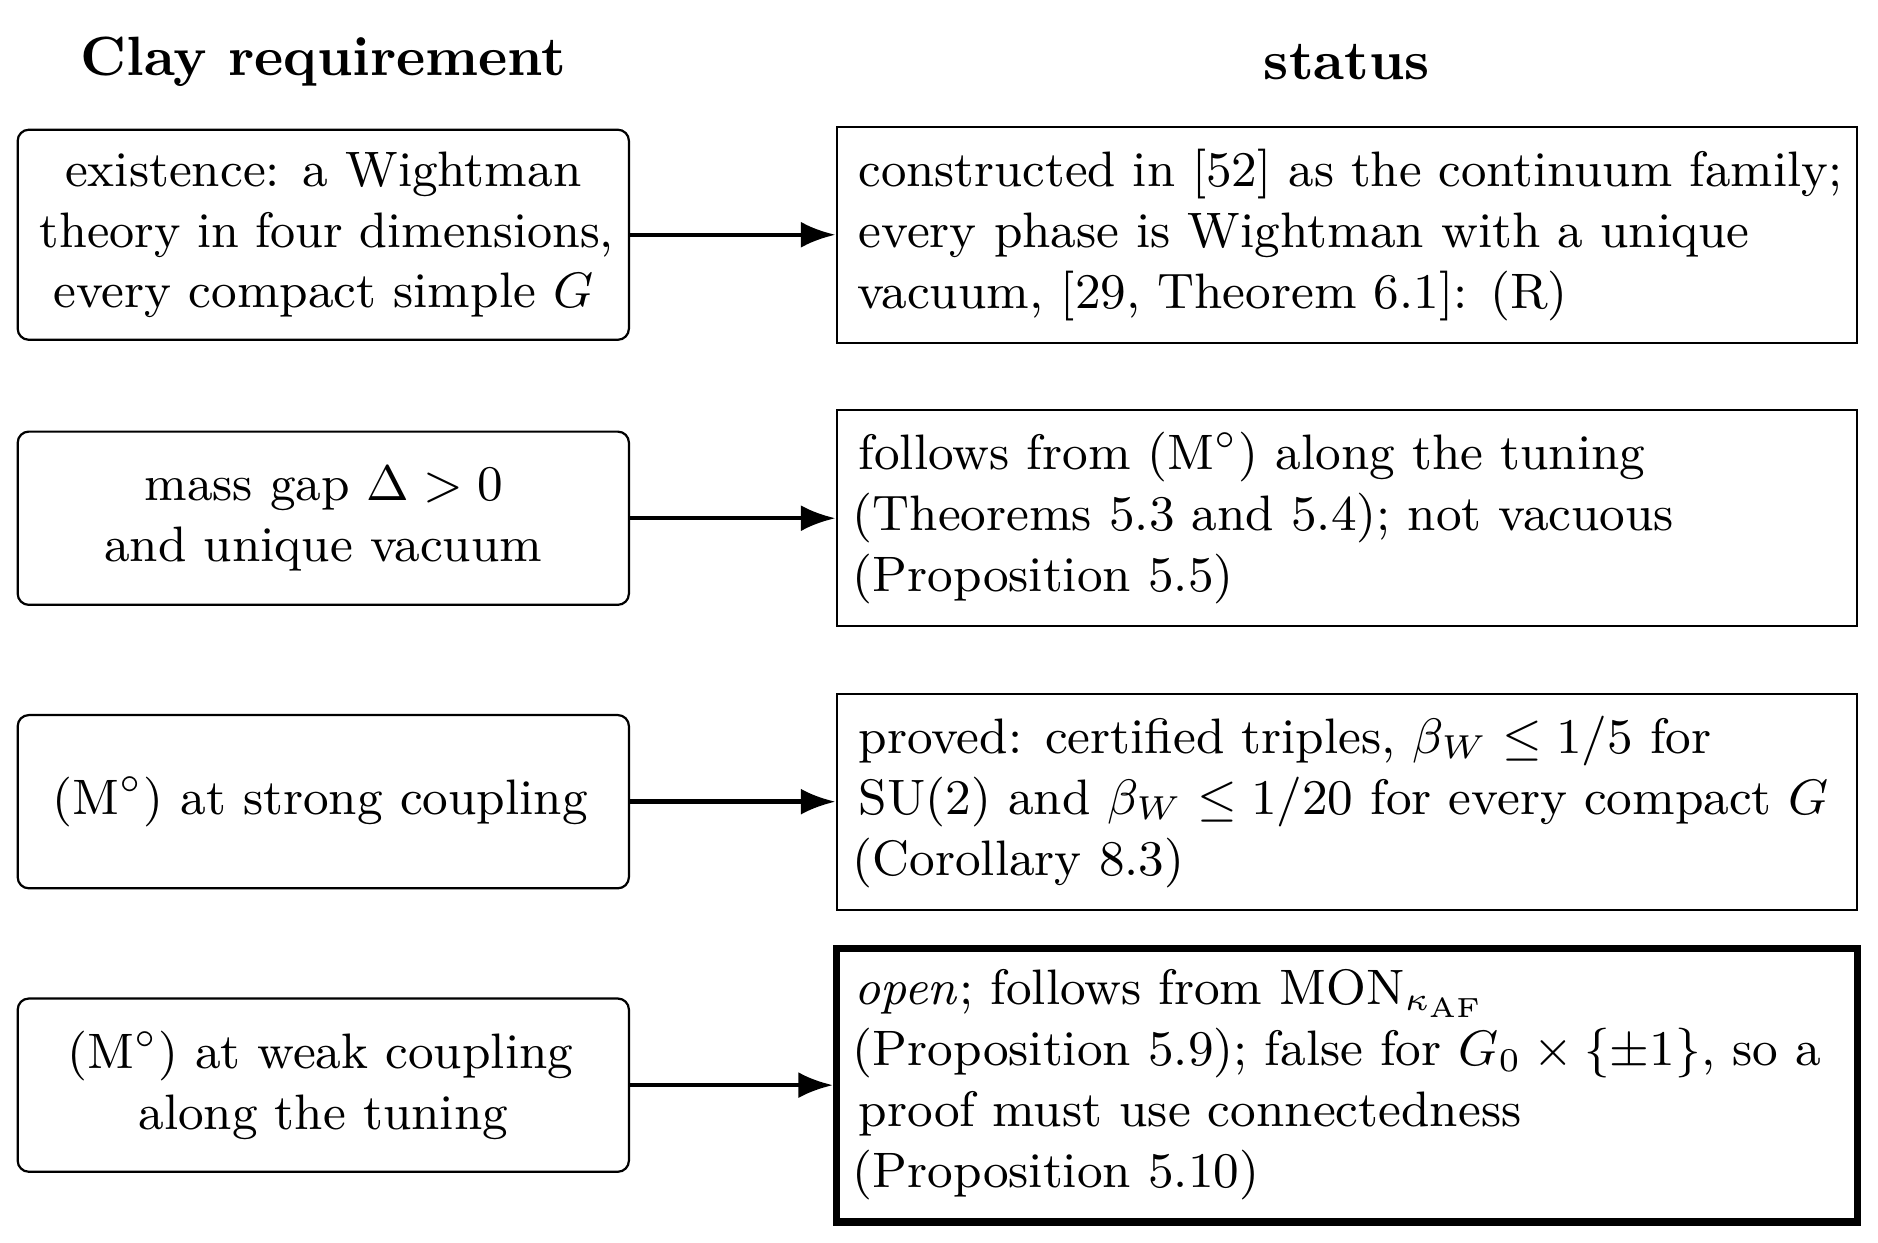
\includegraphics[width=337.9bp]{figures/fig08.png}
\caption{The Clay requirements for the constructed family. Thin boxes state what is proved, in \cite{openaiym,ymgroup2026} or here; the thick box is the one estimate that remains open, and with it the mass gap.}
\label{fig:clay}
\end{figure}
\section{Equivalent single-statement criteria}\label{sec:criteria}

The datum \Mcirc{} compares the partition functions of the tori $\cube{T_0}\times T_0$ and $(2T_0)^4$. This section gives two other forms of it, each a single statement at one scale. The hypercube form \Hcirc{} compares the hypercubes $T_0^4$ and $(2T_0)^4$ and involves no transfer matrix and no vacuum energy (\cref{thm:hypercube}). The Casimir form \Kone+\Ktwo{} puts the tight tolerance on a zero-temperature quantity, the Casimir defect of a cube, and requires only the tolerance $1/300$ for the thermal trace of one hypercube (\cref{thm:casimir-criterion}). Each form implies \Mcirc{} at the same scale, and \Mcirc{} implies each form at twice the scale (\cref{prop:hypercube-converse,thm:casimir-criterion}). As conditions on a continuum family they are therefore equivalent to \Mcirc, with $\tzero$ doubled in one direction: they are reformulations, not weakenings. The tools are the telescoping of the doubling defect (\cref{lem:telescoping}) and a chain of three exchanges of directions that ends in one cold cube (\cref{prop:casimir-chain}).

Throughout, $Z$ is a \PSTS{}. The proofs use (P1), \cref{lem:E1-E3,lem:exchange,lem:purity-conversion} and \cref{thm:cube-control}, so by \cref{lem:simplicity-not-needed} simplicity of $\lzero$ is not used. As in \cref{sec:ascent}, $X(T)=\XT{\cube{T}}{T}$ for integers $T\ge3$, so that \Bcirc{} at $T_0$ reads $X(T_0)\le\xconstinl$. For $n\in\Z^4$ with all $n_\mu\ge3$ let $2n=(2n_1,2n_2,2n_3,2n_4)$, and for integers $T\ge3$ put
\begin{equation}\label{eq:criteria-notation}
\begin{gathered}
\delta(n)=16\log Z(n)-\log Z(2n),\qquad \delta_{\mathrm{hyp}}(T)=\delta(T^4)=16\log Z(T^4)-\log Z\bigl((2T)^4\bigr),\\
X_{\mathrm{hyp}}(T)=\XT{T^3}{T},\qquad \kappa(\cube{T})=E_0(\cube{T})-8E_0(T^3).
\end{gathered}
\end{equation}
Since $\Zs{s}{M}=\Zpart{s}{M}/\lzero(s)^M$ for $M\ge3$,
\begin{equation}\label{eq:logZ-split}
\log\Zpart{s}{M}=-M\,E_0(s)+\XT{s}{M}\qquad(M\ge3).
\end{equation}
The defect $\kappa(\cube{T})$ is the vacuum energy of the cube of side $2T$ minus the vacuum energies of its eight halves; the extensive parts cancel, and in physical units it is a Casimir energy \cite[Proposition~13]{bhattacharjee2026first}. With the free-energy density $f(L)=L^{-4}\log Z(L^4)$ of the hypercube of side $L$, $\delta_{\mathrm{hyp}}(T)=16T^4[f(T)-f(2T)]$.

\subsection{The hypercube form}

\begin{lemma}[{telescoping; \cite[proof of Proposition~16(ii)]{bhattacharjee2026first}}]\label{lem:telescoping}
For every $n\in\Z^4$ with all $n_\mu\ge3$,
\begin{equation}\label{eq:telescoping}
\delta(n)=8\,\psiT{(n_1,n_2,n_3)}{n_4}+4\,\psiT{(n_1,n_2,2n_4)}{n_3}+2\,\psiT{(n_1,2n_3,2n_4)}{n_2}+\psiT{(2n_2,2n_3,2n_4)}{n_1},
\end{equation}
and each purity defect $\psiT{s}{T}$ on the right satisfies $0\le\XT{s}{T}\le\psiT{s}{T}\le2\XT{s}{T}$.
\end{lemma}

\begin{proof}
Let $F=\log Z$, $n^{(0)}=n$, $n^{(1)}=(n_1,n_2,n_3,2n_4)$, $n^{(2)}=(n_1,n_2,2n_3,2n_4)$, $n^{(3)}=(n_1,2n_2,2n_3,2n_4)$ and $n^{(4)}=2n$. For $j=0,1,2,3$ the torus $n^{(j+1)}$ arises from $n^{(j)}$ by doubling the side in the direction $\mu=4-j$, which has length $n_\mu$. Let $u_j$ be the spatial torus formed by the other three sides of $n^{(j)}$:
\[
u_0=(n_1,n_2,n_3),\qquad u_1=(n_1,n_2,2n_4),\qquad u_2=(n_1,2n_3,2n_4),\qquad u_3=(2n_2,2n_3,2n_4).
\]
By (P1), $Z(n^{(j)})=\Zpart{u_j}{n_\mu}$ and $Z(n^{(j+1)})=\Zpart{u_j}{2n_\mu}$, so by \eqref{eq:psi-def}
\[
2F(n^{(j)})-F(n^{(j+1)})=\psiT{u_j}{n_{4-j}}\qquad(j=0,1,2,3).
\]
Multiplying the $j$-th identity by $2^{3-j}$ and adding,
\[
\sum_{j=0}^{3}2^{3-j}\bigl[2F(n^{(j)})-F(n^{(j+1)})\bigr]=\sum_{j=0}^{3}2^{4-j}F(n^{(j)})-\sum_{j=1}^{4}2^{4-j}F(n^{(j)})=16F(n)-F(2n),
\]
which is \eqref{eq:telescoping}. The bounds are \eqref{eq:X-psi} together with $\Zc\ge1$ from (E2).
\end{proof}

The first paper keeps only the first term of \eqref{eq:telescoping}, as a lower bound for $\delta(n)$; this is also how \cref{thm:ascent} uses the lemma, at $n^\circ=(2T_0,2T_0,2T_0,T_0)$, where the first term is $8\psiT{\cube{T_0}}{T_0}$. At the hypercube $n=T_0^4$ the last term is $\psiT{\cube{T_0}}{T_0}$ itself (\cref{fig:telescoping}).

\begin{figure}[htbp]
\centering
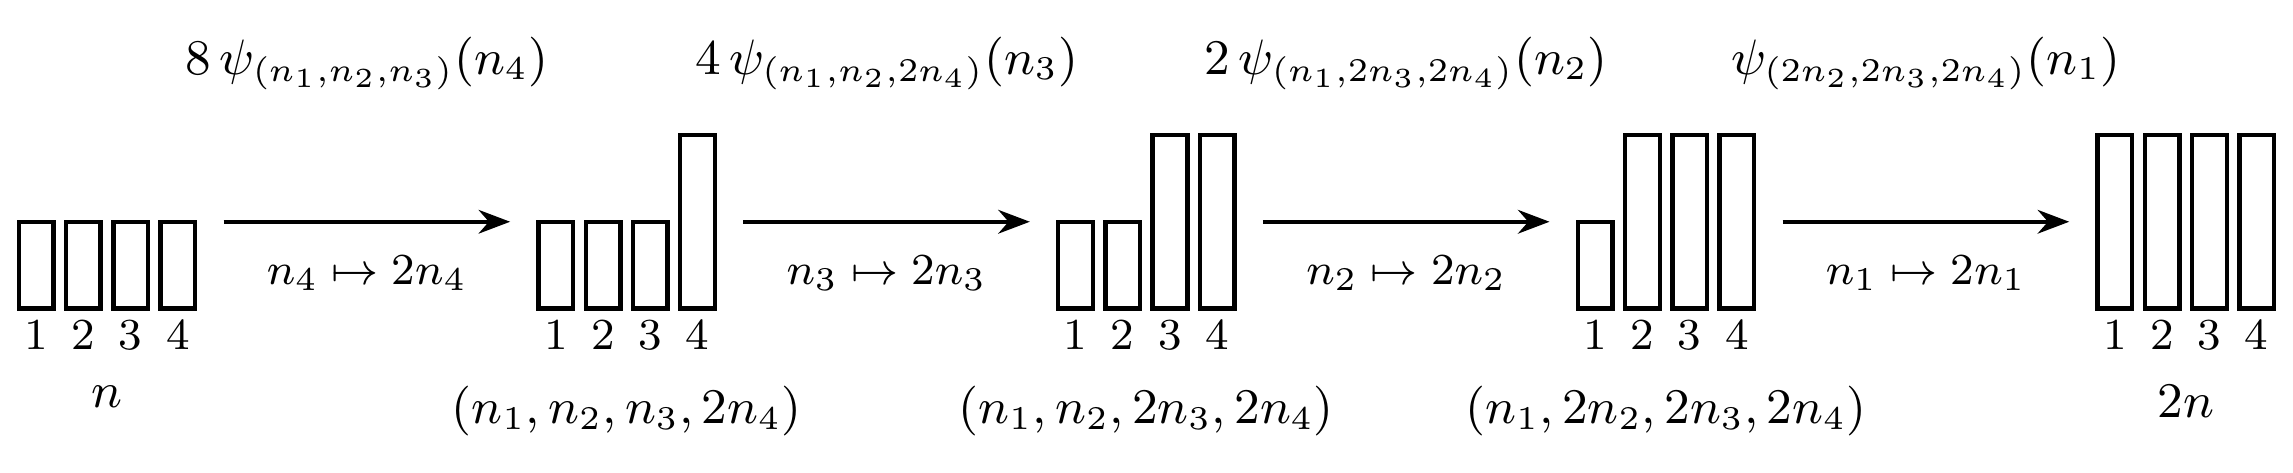
\includegraphics[width=412.7bp]{figures/fig09.png}
\caption{Hypercube telescoping (\cref{lem:telescoping}). Each torus is drawn as four columns, one for each of the directions $1,2,3,4$; a tall column is a doubled side. Each arrow doubles one side, and the purity defect attached to it reads the doubled direction as time and the other three sides as the spatial torus. With the weights $8,4,2,1$ the four terms add up to $\delta(n)=16\log Z(n)-\log Z(2n)$. At the hypercube $n=T_0^4$ the last term is $\psiT{\cube{T_0}}{T_0}$, the quantity bounded in \Mcirc{} (\cref{thm:hypercube}).}
\label{fig:telescoping}
\end{figure}

Let $T_0\ge3$ be an integer. The system satisfies \Hcirc{} at $T_0$ if
\begin{equation}\label{eq:datum-H}
\delta_{\mathrm{hyp}}(T_0)=16\log Z(T_0^4)-\log Z\bigl((2T_0)^4\bigr)\le\dconst,
\end{equation}
that is, $Z(T_0^4)^{16}\le e^{\dconstinl}Z((2T_0)^4)$.
For a continuum family we use the convention of \cref{sec:psts}: \Hcirc{} holds \emph{along the tuning} with $\tzero>0$ if for every sufficiently large $p$ there is $N_0(p)$ such that for every $N\ge N_0(p)$ the Wilson system at $\betaNp$ satisfies \Hcirc{} at some integer $T_0$ with $3\le T_0\le N\tzero$. The conditions \Kone+\Ktwo{} below are taken along the tuning in the same way, both at one integer $L$ with $3\le L\le N\tzero$, and so is \textup{(K$^\circ$)}, at one integer $T_0$ with $3\le T_0\le N\tzero$.

\begin{theorem}[hypercube criterion]\label{thm:hypercube}
Let $T_0\ge3$. If $Z$ satisfies \Hcirc{} at $T_0$, then
\[
\XT{\cube{T_0}}{T_0}\le\psiT{\cube{T_0}}{T_0}\le\delta_{\mathrm{hyp}}(T_0)\le\dconst ,
\]
so $Z$ satisfies \Mcirc{} at $T_0$, and by \cref{lem:purity-conversion} also \Bcirc{} at $T_0$. If a continuum family satisfies \Hcirc{} along the tuning with $\tzero$, then it satisfies \Mcirc{} along the tuning with the same $\tzero$; if it satisfies moreover \UVB{} or \hypW, the conclusions \textup{(i)}--\textup{(iii)} of \cref{thm:main} hold with $\Delta=\tzero^{-1}\log\frac{63}{32}>0.677/\tzero$.
\end{theorem}

\begin{proof}
\Cref{lem:telescoping} at $n=T_0^4$ has $2n=(2T_0)^4$, and its last term is $\psiT{(2T_0,2T_0,2T_0)}{T_0}=\psiT{\cube{T_0}}{T_0}$. The other three terms are nonnegative, so $\psiT{\cube{T_0}}{T_0}\le\delta_{\mathrm{hyp}}(T_0)\le\dconstinl$, which is \Mcirc{} at $T_0$; the first inequality of the display is \eqref{eq:X-psi}. Along the tuning the witness $T_0$ does not change, so \Mcirc{} holds along the tuning with $\tzero$, and \cref{thm:main} applies with this $\tzero$.
\end{proof}

\Hcirc{} is a statement about the free-energy densities of two hypercubic tori, $16T_0^4[f(T_0)-f(2T_0)]\le\dconstinl$. It is symmetric in the four directions and contains no transfer matrix, vacuum energy or thermal trace. The last sentence of \cref{thm:ascent} uses the coefficient-$8$ term of \eqref{eq:telescoping} at $n^\circ$ and needs the tolerance $1/1024$ there; \cref{thm:hypercube} uses the coefficient-$1$ term at the hypercube.

\begin{proposition}[converse]\label{prop:hypercube-converse}
Let $T_0\ge3$, and suppose that $Z$ satisfies \Bcirc{} at $T_0$. Then
\begin{equation}\label{eq:hypercube-converse}
\delta_{\mathrm{hyp}}(2T_0)\le\frac{16}{8191^2}+\frac{8}{511^2}+\frac{4}{255^2}+\frac{2}{127^2}<2.17\cdot10^{-4}<\dconst ,
\end{equation}
so $Z$ satisfies \Hcirc{} at $2T_0$. Consequently, a continuum family that satisfies \Mcirc{} along the tuning with $\tzero$ satisfies \Hcirc{} along the tuning with $2\tzero$, and a family satisfies \Hcirc{} along the tuning for some $\tzero>0$ if and only if it satisfies \Mcirc{} along the tuning for some $\tzero>0$.
\end{proposition}

\begin{proof}
Put $L=2T_0$ and $x_0=\xconstinl$. \Cref{lem:telescoping} at $n=L^4$ gives
\[
\delta_{\mathrm{hyp}}(L)=8\,\psiT{t_1}{L}+4\,\psiT{t_2}{L}+2\,\psiT{t_3}{L}+\psiT{t_4}{L},
\]
with $t_1=(L,L,L)$, $t_2=(L,L,2L)$, $t_3=(L,2L,2L)$ and $t_4=(2L,2L,2L)$. All sides of these tori are at least $2T_0$, and $\Vol{t_j}/T_0^3=k_j$ with $(k_1,k_2,k_3,k_4)=(8,16,32,64)$. For $t_1=\cube{T_0}$, $\log\Zs{t_1}{T_0}=X(T_0)\le x_0$ by \Bcirc{}; for $j=2,3,4$, \eqref{eq:cube-control} gives $\log\Zs{t_j}{T_0}\le k_jX(T_0)\le k_jx_0$. By $e^y-1\le y/(1-y)$ for $0\le y<1$, which follows from $e^{-y}\ge1-y$,
\[
\Dexc{t_1}{T_0}\le e^{x_0}-1\le\frac1{8191},\qquad \Dexc{t_j}{T_0}\le e^{k_jx_0}-1\le\frac{k_j}{8192-k_j}\qquad(j=2,3,4),
\]
and $k_j/(8192-k_j)$ equals $1/511$, $1/255$, $1/127$ for $j=2,3,4$. By \eqref{eq:X-psi}, $\log(1+y)\le y$ and (E2) with $M'=M''=T_0$,
\[
\psiT{t_j}{2T_0}\le2\,\XT{t_j}{2T_0}\le2\,\Dexc{t_j}{2T_0}\le2\,\Dexc{t_j}{T_0}^2\qquad(j=1,2,3,4).
\]
Summing with the weights $8,4,2,1$ gives the first inequality of \eqref{eq:hypercube-converse}. The sum is less than $2.1640\cdot10^{-4}$, and $\dconstinl>2.4408\cdot10^{-4}$ (\cref{app:certificates}).

If \Mcirc{} holds along the tuning with $\tzero$, then for all large $p$ and $N\ge N_0(p)$ some integer $3\le T_0\le N\tzero$ satisfies \Mcirc, hence \Bcirc{} by \cref{lem:purity-conversion}, hence \Hcirc{} at $2T_0$, and $3\le2T_0\le N\cdot2\tzero$. With \cref{thm:hypercube} this gives the equivalence.
\end{proof}

At one scale \Hcirc{} is stronger than \Mcirc, because $\psiT{\cube{T_0}}{T_0}\le\delta_{\mathrm{hyp}}(T_0)$; the converse is paid for by doubling the scale. The factor between the two can be $4$. In the product of rings $Z(n)=\prod_{\mu=1}^4(1+r^{n_\mu})^{|n|/n_\mu}$, $0<r<1$, described after \cref{thm:upward-closed}, $\log Z(T^4)=4T^3\log(1+r^T)$ and $\Zs{s}{T}=(1+r^T)^{\Vol{s}}$, so
\[
\delta_{\mathrm{hyp}}(T)=64T^3\log(1+r^T)-32T^3\log(1+r^{2T})=4\,\psiT{\cube{T}}{T}\qquad(T\ge3),
\]
and \Hcirc{} at $T_0$ is the condition $\psiT{\cube{T_0}}{T_0}\le1/16\,388$.

\subsection{The Casimir form}

The second form separates the datum into a vacuum-energy part and a thermal part. It rests on three exchanges of directions, each of which halves one side of the cube $\cube{T}$ and doubles the time.

\begin{proposition}[cold-cube chain and Casimir identity]\label{prop:casimir-chain}
Let $T\ge3$, and put
\begin{align*}
b_1&=T\bigl[E_0(\cube{T})-2E_0(T,2T,2T)\bigr], & b_2&=T\bigl[E_0(T,2T,2T)-2E_0(T,T,2T)\bigr],\\
b_3&=T\bigl[E_0(T,T,2T)-2E_0(T^3)\bigr].
\end{align*}
\begin{enumerate}[label=(\alph*)]
\item $b_1,b_2,b_3\ge0$ and $b_1+2b_2+4b_3=T\kappa(\cube{T})$; in particular $\kappa(\cube{T})\ge0$ (this is also \cite[Proposition~13]{bhattacharjee2026first}).
\item $X(T)\le b_1+b_2+b_3+\XT{T^3}{2T}\le T\kappa(\cube{T})+\XT{T^3}{2T}$.
\item $\delta_{\mathrm{hyp}}(T)=2T\kappa(\cube{T})+16X_{\mathrm{hyp}}(T)-X_{\mathrm{hyp}}(2T)$.
\item $X(T)\le\delta_{\mathrm{hyp}}(T)-14X_{\mathrm{hyp}}(T)$.
\end{enumerate}
\end{proposition}

\begin{proof}
Let $b,c\ge3$. In \cref{lem:exchange}, $g(\ell)=\log\lzero(\ell,b,c)=-E_0(\ell,b,c)$ and $\zeta(\ell)=g(\ell)-\ell\bar e$, so $\delta_T=2\zeta(T)-\zeta(2T)=2g(T)-g(2T)=E_0(2T,b,c)-2E_0(T,b,c)$. Part (c) of that lemma therefore reads
\begin{equation}\label{eq:doubling-step}
\begin{gathered}
\log\Zs{(2T,b,c)}{T}=\log\Zs{(T,b,c)}{2T}+T\bigl[E_0(2T,b,c)-2E_0(T,b,c)\bigr],\\
E_0(2T,b,c)-2E_0(T,b,c)\ge\zeta(T)\ge0 .
\end{gathered}
\end{equation}
The inequality is the doubling case of the superadditivity of $\ell\mapsto E_0(\ell,b,c)$ \cite[Lemma~28(ii)]{bhattacharjee2026first}. By (E1), $E_0(s)$ and $\Zs{s}{M}$, $M\ge3$, are invariant under permutations of the sides of $s$; by (E2), $\Zs{s}{M}$ is nonincreasing in $M$.

(a) Since $E_0(T,2T,2T)=E_0(2T,T,2T)$ and $E_0(T,T,2T)=E_0(2T,T,T)$, the numbers $b_1$, $b_2$, $b_3$ are $T[E_0(2T,b,c)-2E_0(T,b,c)]$ for $(b,c)=(2T,2T)$, $(T,2T)$ and $(T,T)$ respectively, so they are nonnegative by \eqref{eq:doubling-step}. The sum $b_1+2b_2+4b_3$ telescopes to $T[E_0(\cube{T})-8E_0(T^3)]=T\kappa(\cube{T})$.

(b) The three equalities below are \eqref{eq:doubling-step} with $(b,c)=(2T,2T)$, $(T,2T)$ and $(T,T)$, and each inequality permutes the sides and lowers the time from $2T$ to $T$:
\begin{align*}
X(T)=\log\Zs{(2T,2T,2T)}{T}&=b_1+\log\Zs{(T,2T,2T)}{2T}\le b_1+\log\Zs{(2T,T,2T)}{T}\\
&=b_1+b_2+\log\Zs{(T,T,2T)}{2T}\le b_1+b_2+\log\Zs{(2T,T,T)}{T}\\
&=b_1+b_2+b_3+\XT{T^3}{2T}.
\end{align*}
The second inequality of (b) follows from $b_2\le2b_2$, $b_3\le4b_3$ and (a).

(c) By \eqref{eq:logZ-split} with $(s,M)=(T^3,T)$ and with $(s,M)=(\cube{T},2T)$,
\[
16\log Z(T^4)-\log Z\bigl((2T)^4\bigr)=16X_{\mathrm{hyp}}(T)-16T\,E_0(T^3)-X_{\mathrm{hyp}}(2T)+2T\,E_0(\cube{T}),
\]
which is (c).

(d) By (b) and the monotonicity in time, $X(T)\le T\kappa(\cube{T})+X_{\mathrm{hyp}}(T)$. By (c), $T\kappa(\cube{T})=\frac12\bigl[\delta_{\mathrm{hyp}}(T)-16X_{\mathrm{hyp}}(T)+X_{\mathrm{hyp}}(2T)\bigr]$, and $X_{\mathrm{hyp}}(2T)=\XT{\cube{T}}{2T}\le\XT{\cube{T}}{T}=X(T)$. Hence $X(T)\le\frac12\delta_{\mathrm{hyp}}(T)-7X_{\mathrm{hyp}}(T)+\frac12X(T)$, and since $X(T)$ is finite this is (d).
\end{proof}

The halving inequality \cite[Proposition~13]{bhattacharjee2026first} compares the cube of side $2T$ with its eight halves at times $M'$, $M''$ with $M'+M''=T$, and leaves the remainder $\sum_s\Dexc{s}{M'}\Dexc{s}{M''}$ over eight copies $s$ of $T^3$. In (b) the exchanges convert side length into time, and the remainder is the free energy $\XT{T^3}{2T}$ of one cube $T^3$ at the time $2T$, which by $\log(1+y)\le y$ and (E2) is at most $\Dexc{T^3}{T}^2$. Part (d) shows that the hypercube defect dominates $X(T)$ with the correction $-14X_{\mathrm{hyp}}(T)\le0$; in particular $\delta_{\mathrm{hyp}}(T_0)\le\xconstinl$ gives \Bcirc{} at $T_0$ directly.

Let $L\ge3$ be an integer. The system satisfies \Kone{} and \Ktwo{} at $L$ if
\begin{equation}\label{eq:datum-K}
\begin{aligned}
&\Kone\qquad L\,\kappa(\cube{L})=L\bigl[E_0(\cube{L})-8E_0(L^3)\bigr]\le\frac{11}{10^5},\\
&\Ktwo\qquad X_{\mathrm{hyp}}(L)=\XT{L^3}{L}\le\frac1{300}.
\end{aligned}
\end{equation}
\Kone{} concerns vacuum energies only, and \Ktwo{} is the thermal trace of the hypercube $L^4$ at aspect ratio one, with a tolerance more than $27$ times that of \Bcirc. The system satisfies \textup{(K$^\circ$)} at $T_0\ge3$ if $T_0\kappa(\cube{T_0})+\XT{T_0^3}{2T_0}\le\xconstinl$.

\begin{theorem}[Casimir criterion]\label{thm:casimir-criterion}
Let $Z$ be a \PSTS{}.
\begin{enumerate}[label=(\alph*)]
\item If $Z$ satisfies \Kone{} and \Ktwo{} at an integer $L\ge3$, then
\[
X(L)\le\frac{11}{10^5}+\frac1{299^2}\le1.21186\cdot10^{-4}<\xconst,\qquad \psiT{\cube{L}}{L}\le2X(L)<\dconst ,
\]
so $Z$ satisfies \Bcirc{} and \Mcirc{} at $L$.
\item If $Z$ satisfies \Bcirc{} at $T_0\ge3$, then $L=2T_0$ satisfies
\[
L\,\kappa(\cube{L})\le\frac1{127^2}+\frac2{255^2}+\frac4{511^2}<1.081\cdot10^{-4},\qquad X_{\mathrm{hyp}}(L)\le\frac1{8191^2},
\]
so $Z$ satisfies \Kone{} and \Ktwo{} at $2T_0$.
\item If $Z$ satisfies \textup{(K$^\circ$)} at $T_0\ge3$, then it satisfies \Bcirc{} at $T_0$. If $Z$ satisfies \Bcirc{} at $T_0\ge3$, then $L=2T_0$ satisfies $L\kappa(\cube{L})+\XT{L^3}{2L}<1.081\cdot10^{-4}+8191^{-4}<\xconstinl$, so \textup{(K$^\circ$)} holds at $2T_0$.
\item If a continuum family satisfies \Kone{} and \Ktwo{} along the tuning with $\tzero$, then it satisfies \Mcirc{} along the tuning with the same $\tzero$; if it satisfies moreover \UVB{} or \hypW, the conclusions \textup{(i)}--\textup{(iii)} of \cref{thm:main} hold with $\Delta=\tzero^{-1}\log\frac{63}{32}>0.677/\tzero$. If the family satisfies \Mcirc{} along the tuning with $\tzero$, then it satisfies \Kone{} and \Ktwo{} along the tuning with $2\tzero$.
\end{enumerate}
\end{theorem}

\begin{proof}
(a) By \cref{prop:casimir-chain}(b) at $T=L$, $X(L)\le L\kappa(\cube{L})+\XT{L^3}{2L}$. By $\log(1+y)\le y$ and (E2), $\XT{L^3}{2L}\le\Dexc{L^3}{2L}\le\Dexc{L^3}{L}^2$, and by \Ktwo{} and $e^y-1\le y/(1-y)$, $\Dexc{L^3}{L}=e^{X_{\mathrm{hyp}}(L)}-1\le e^{1/300}-1\le1/299$. With \Kone,
\[
X(L)\le\frac{11}{10^5}+\frac1{299^2}=\frac{1\,083\,411}{8\,940\,100\,000}.
\]
This is at most $1.21186\cdot10^{-4}$ and less than $\xconstinl$, because $8192\cdot1\,083\,411=8\,875\,302\,912<8\,940\,100\,000$. By \eqref{eq:X-psi}, $\psiT{\cube{L}}{L}\le2X(L)\le1\,083\,411/4\,470\,050\,000<\dconstinl$, because $4097\cdot1\,083\,411=4\,438\,734\,867<4\,470\,050\,000$.

(b) Let $L=2T_0$. By \cref{prop:casimir-chain}(a) at $T=L$, $L\kappa(\cube{L})=b_1+2b_2+4b_3$. By \eqref{eq:doubling-step}, the permutation invariance of $\Zc$ and $\Zc\ge1$,
\begin{gather*}
b_1=\log\Zs{(2L,2L,2L)}{L}-\log\Zs{(L,2L,2L)}{2L}\le\log\Zs{(2L,2L,2L)}{L},\\
b_2=\log\Zs{(2L,L,2L)}{L}-\log\Zs{(L,L,2L)}{2L}\le\log\Zs{(L,2L,2L)}{L},\\
b_3=\log\Zs{(2L,L,L)}{L}-\log\Zs{(L,L,L)}{2L}\le\log\Zs{(L,L,2L)}{L}.
\end{gather*}
These are the tori $t_4$, $t_3$, $t_2$ of the proof of \cref{prop:hypercube-converse} at the time $L=2T_0$, and as there $\log\Zs{t_j}{2T_0}\le\Dexc{t_j}{2T_0}\le\Dexc{t_j}{T_0}^2$ with $\Dexc{t_4}{T_0}\le1/127$, $\Dexc{t_3}{T_0}\le1/255$, $\Dexc{t_2}{T_0}\le1/511$. Hence $b_1\le1/127^2$, $b_2\le1/255^2$, $b_3\le1/511^2$, and
\[
L\kappa(\cube{L})\le\frac1{127^2}+\frac2{255^2}+\frac4{511^2}<1.0808\cdot10^{-4}<\frac{11}{10^5}.
\]
Finally $X_{\mathrm{hyp}}(L)=\XT{\cube{T_0}}{2T_0}\le\Dexc{\cube{T_0}}{2T_0}\le\Dexc{\cube{T_0}}{T_0}^2\le(e^{x_0}-1)^2\le8191^{-2}<1/300$, with $x_0=\xconstinl$.

(c) The first claim is \cref{prop:casimir-chain}(b) at $T=T_0$. For the second, (b) gives $L\kappa(\cube{L})<1.0808\cdot10^{-4}$, and $\log(1+y)\le y$ and (E2), applied twice, give $\XT{L^3}{2L}=\XT{\cube{T_0}}{4T_0}\le\Dexc{\cube{T_0}}{4T_0}\le\Dexc{\cube{T_0}}{T_0}^4\le8191^{-4}$. The sum is less than $1.0809\cdot10^{-4}<\xconstinl$.

(d) The witness $L$, $3\le L\le N\tzero$, satisfies \Mcirc{} by (a), so \Mcirc{} holds along the tuning with $\tzero$ and \cref{thm:main} applies. Conversely, a witness $T_0\le N\tzero$ of \Mcirc{} satisfies \Bcirc{} by \cref{lem:purity-conversion}, and by (b) the integer $2T_0$, with $3\le2T_0\le N\cdot2\tzero$, satisfies \Kone{} and \Ktwo.
\end{proof}

\Kone{} alone does not imply \Mcirc{} in the class of all \PSTS{}. For $0<q<1$ the system $Z(n)=1+q^{|n|}$ has $\TT_s=\mathrm{diag}(1,q^{\Vol{s}})$ (\cref{prop:gapless-sector}), so $\lzero(s)=1$ and $E_0\equiv0$ for every $s$; thus $\kappa\equiv0$ and \Kone{} holds at every $L\ge3$. With $q_N=e^{-N^{-5}}$ the family is in alternative (I) of \cref{thm:zero-one}, as shown in the remark after that theorem, so \Mcirc{} fails along it for every $\tzero$. Whether \Ktwo{}, with some fixed tolerance, implies \Mcirc{} in every \PSTS{} is not decided here; by \cref{prop:casimir-chain}(b), what \Ktwo{} lacks for \Bcirc{} at the same scale is the Casimir term $L\kappa(\cube{L})$.

\smallskip
\noindent\emph{Remark.} Each of \Hcirc, \Kone+\Ktwo{} and \textup{(K$^\circ$)} at a scale implies \Bcirc{} at that scale, the first two even \Mcirc, and \Bcirc{} at $T_0$ implies each of them at $2T_0$. As conditions on a family, each is therefore equivalent to \Mcirc{} up to the replacement of $\tzero$ by $2\tzero$ (for \textup{(K$^\circ$)} via \Bcirc{} at $T_0$ $\Rightarrow$ \Hcirc{} at $2T_0$ $\Rightarrow$ \Mcirc{} at $2T_0$, \cref{prop:hypercube-converse,thm:hypercube}), and none of them defines a larger class of theories. What changes is the quantity that carries the smallness: in \Hcirc{} it is a difference of two hypercubic free energies, in \Kone{} the zero-temperature Casimir defect of a cube of physical side at most $2\tzero$, while the thermal part \Ktwo{} needs only the tolerance $1/300$. Since each criterion implies \Bcirc{} at the same scale, the necessary conditions on \Bcirc{} in \cref{sec:necessary}, such as the spectral conditions of \cref{prop:spectral-conditions} and the growth of the base scale in \cref{cor:base-scale}(c), apply to each of them at that scale. All the criteria are Euclidean statements about the partition function.\footnote{A Hamiltonian form is not needed for the Clay statement and is not used in this paper. Let $H_{\mathrm{KS}}=\frac{g^2}{2}\sum_eE_e^2+\frac{2}{g^2}\sum_p(N_c-\ReTr Q_p)$ be the Kogut--Susskind Hamiltonian \cite{kogut1975} on the gauge-invariant functions of the spatial links of the cube $\cube{T_0}$, where $E_e^2$ is the quadratic Casimir operator acting on the variable of the link $e$, and let $\varepsilon_0\le\varepsilon_1\le\dots$ be its eigenvalues counted with multiplicity and $\Delta_{\mathrm{KS}}=\varepsilon_1-\varepsilon_0$. The condition $\log\Tr e^{-T_0(H_{\mathrm{KS}}-\varepsilon_0)}\le\xconstinl$ gives $1+e^{-T_0\Delta_{\mathrm{KS}}}\le e^{\xconstinl}$, hence $T_0\Delta_{\mathrm{KS}}\ge-\log(e^{\xconstinl}-1)>9.0108>9.01$ (\cref{app:certificates}). No relation between the gap of the isotropic Wilson transfer matrix and the Kogut--Susskind gap is proved in either direction.\label{fn:kogut-susskind}} Neither \Hcirc{} nor \Kone+\Ktwo{} is proved along the continuum tuning; every continuum statement of this section is conditional on \UVB{} or \hypW{} and on the criterion assumed.
\section{Centre grading: electric-flux residue, rotation identity, projected split}\label{sec:centre}

The centre of the gauge group grades the space of a time slice into electric-flux sectors \cite{thooft1979}. In \cite{bhattacharjee2026first} the centre flips of the links crossing one coordinate plane enter the upper bound on the gap of a fixed torus (\cref{lem:fp-slice,thm:fp-fixed-size}); here the same flips grade the datum itself. This section splits the free energy of the datum along the grading into a centre-neutral part and an electric-flux residue (\cref{thm:residue-split}); on the cube of the datum the residue is one flux weight on a crossed box (\cref{fig:rotation}). The split holds for every finite symmetry group of the transfer matrix (\cref{thm:projected-split}), and neither part controls the other (\cref{prop:no-residue-control}). \Cref{prop:polyakov-bound,thm:magnetic-P,thm:flux-count,cor:neutral-threshold} relate the residue conditions \hypN{} and \hypP{} of \eqref{eq:cg-NP} to Polyakov loops, magnetic flux energies, flux states and neutral excitations. Neither \hypN{} nor \hypP{} is proved at any weak coupling along the continuum tuning.

\subsection{Centre operators and twisted partition functions}

Throughout this section $G\subset\U(N_c)$ is closed, $f\in\Fclass(G)$, and $Z$ is the system of \cref{prop:class-weight-psts}; Wilson theory is the case $f(g)=\exp(N_c\beta\ReTr g)$. The prefactor $(\min f)^{-6|n|}$ changes no normalised quantity and no ratio below, and we omit it: $Z(n)=\int\prod_pf(Q_p)\prod_{(x,\mu)}\dd U_{(x,\mu)}$. The transfer matrix $\TT_s$ on $\Kspace_s=L^2(G^{E_s})$ has the kernel
\begin{equation}\label{eq:cg-kernel}
\TT_s(Q,Q')=\int_{G^{\Lambda_s}}\prod_pf(Q_p)^{1/2}f(Q'_p)^{1/2}\prod_{x\in\Lambda_s}\prod_{i=1}^3f\bigl(Q_{(x,i)}U_{x+e_i}Q'^*_{(x,i)}U_x^*\bigr)\prod_{x}\dd U_x ,
\end{equation}
$p$ running over the plaquettes of $\Lambda_s$, and \cref{lem:transfer-matrix}\textup{(i)--(iv)} hold for it.

Let $C$ be a finite subgroup of the centre of $G$, for instance $C=\{\omega^a\}\cong\Z_{N_c}$, $\omega=e^{2\pi i/N_c}$, for $G=\SU(N_c)$. Elements $k=(k_1,k_2,k_3)\in C^3$ are written multiplicatively, characters $e=(e_1,e_2,e_3)\in\widehat C^{\,3}$ additively with $0$ the trivial character, and $e(k)=\prod_je_j(k_j)$; for $\kappa\in C$, $\kappa_{(j)}\in C^3$ has $\kappa$ in place $j$ and $1$ elsewhere. For $\SU(N_c)$ we write $k$ and $e$ additively in $\Z_{N_c}^3$, so that $e(k)=\omega^{e\cdot k}$. With the operators $z_j^c$ of \cref{sec:psts} put $\zeta^k=\zeta_1^{k_1}\zeta_2^{k_2}\zeta_3^{k_3}$, $(z^kh)(Q)=h(\zeta^kQ)$, and for $T\ge3$
\begin{equation}\label{eq:cg-sectors}
P_e=\abs{C}^{-3}\sum_{k\in C^3}\overline{e(k)}\,z^k,\qquad Z_s(T;k)=\Tr(z^k\TT_s^T),\qquad Z^e_s(T)=\Tr(P_e\TT_s^T),
\end{equation}
$\Kspace^e_s=P_e\Kspace_s$, $w_e(s,T)=Z^e_s(T)/\Zpart{s}{T}$ and $\Zc^e_s(T)=\Tr(P_eR_s^T)$. These are 't Hooft's twisted partition functions and electric-flux weights \cite{thooft1979}.

\emph{Twisted integrals.} For $1\le\mu<\nu\le4$ and $(a,b)\in\Z/n_\mu\Z\times\Z/n_\nu\Z$ the \emph{stack} $\Sigma_{\mu\nu}(a,b)$ is the set of $(\mu,\nu)$-plaquettes whose base point $x$ has $x_\mu=a$ and $x_\nu=b$, with $Q_p$ oriented as in \cref{sec:psts}, $\mu$ before $\nu$; it contains one plaquette for each point of the transverse two-torus. For $\gamma=(\gamma_{\mu\nu})_{\mu<\nu}\in C^6$ and a choice of one stack in each plane, let $\eta_p=\gamma_{\mu\nu}$ on the chosen $(\mu,\nu)$-stack and $\eta_p=1$ on all other plaquettes, and
\begin{equation}\label{eq:cg-twisted}
Z(n;\gamma)=\int\prod_pf(\eta_pQ_p)\prod_{(x,\mu)}\dd U_{(x,\mu)} .
\end{equation}
As $f$ is a class function and $\eta_p$ is central, $f(\eta_pQ_p)$ does not depend on the base point of $p$; reversing the orientation of $p$ replaces it by $f(\eta_p^{-1}Q_p)$, since $f(g^{-1})=f(g)$. For $m=(m_{ab})_{1\le a<b\le3}\in C^3$ let $\eta^{(m)}_p=m_{ab}$ for the plaquettes $p$ of $\Lambda_s$ in the $(a,b)$-plane with base point $x_a=x_b=0$ and $\eta^{(m)}_p=1$ otherwise, and let $\TT_s^{(m)}$ be the operator with kernel \eqref{eq:cg-kernel} in which $f(Q_p)^{1/2}f(Q'_p)^{1/2}$ is replaced by $f(\eta^{(m)}_pQ_p)^{1/2}f(\eta^{(m)}_pQ'_p)^{1/2}$; thus $\TT_s^{(1)}=\TT_s$.

\begin{lemma}[centre operators and twists]\label{lem:centre-operators}
Let $s$ be a spatial torus and $T\ge3$.
\begin{enumerate}[label=\textup{(\alph*)},leftmargin=*]
\item $k\mapsto z^k$ is a unitary representation of $C^3$ on $\Kspace_s$ which commutes with $\TT_s$ and with every $R_U$. The $P_e$ are orthogonal projections commuting with $\TT_s$ and every $R_U$, $P_eP_{e'}=0$ for $e\ne e'$, $\sum_eP_e=1$ and $z^k=\sum_ee(k)P_e$. Moreover $\Omegazero\in\Kspace^0_s$, $Z^e_s(T)\ge0$ and $Z^0_s(T)\ge\lzero(s)^T$.
\item For $m\in C^3$, $\TT^{(m)}_s=D_m\Pi K\Pi D_m\ge0$, where $D_m$ is multiplication by $\prod_pf(\eta^{(m)}_pQ_p)^{1/2}$ and $K=\bigotimes_eC_f$; \cref{lem:transfer-matrix}\textup{(i),(ii)} hold for $\TT^{(m)}_s$, and it commutes with every $z^k$ and every $R_U$. For $k\in C^3$ and $M\ge3$
\begin{equation}\label{eq:cg-trace}
\Tr\bigl(z^k(\TT^{(m)}_s)^M\bigr)=Z\bigl((s,M);\gamma\bigr),\qquad \gamma_{j4}=k_j,\quad\gamma_{ab}=m_{ab}\ \ (a<b\le3),
\end{equation}
with the stacks $\Sigma_{j4}(0,M-1)$ and $\Sigma_{ab}(0,0)$. Every $Z(n;\gamma)$ is independent of the choice of the stacks.
\item $Z_s(T;k)$ is the integral \eqref{eq:cg-twisted} on $(s,T)$ with $\gamma_{j4}=k_j$ and $\gamma=1$ on the spatial planes. It is real, $0<Z_s(T;k)=Z_s(T;k^{-1})\le\Zpart{s}{T}$, and
\begin{equation}\label{eq:cg-duality}
Z_s(T;k)=\sum_ee(k)\,Z^e_s(T),\qquad Z^e_s(T)=\abs{C}^{-3}\sum_k\overline{e(k)}\,Z_s(T;k).
\end{equation}
\item Let $i\ne j$ in $\{1,2,3\}$ and $\kappa\in C$, let $s^{(i)}$ be $s$ with $s_i$ replaced by $T$, and let $\TT_\kappa=\TT^{(m)}_{s^{(i)}}$ with $m_{ab}=\kappa$ for $\{a,b\}=\{i,j\}$ and $m_{ab}=1$ for the two other planes. Then $Z_s(T;\kappa_{(j)})=\Tr\TT_\kappa^{s_i}$ and $\lzero(\TT_\kappa)\le\lzero(s^{(i)})$.
\end{enumerate}
\end{lemma}

\begin{proof}
(a) The maps $\zeta_j^c$ preserve Haar measure, $\zeta_j^c\zeta_j^{c'}=\zeta_j^{cc'}$, and $\zeta_j^c$, $\zeta_{j'}^{c'}$ act on disjoint sets of links for $j\ne j'$; so $k\mapsto z^k$ is a unitary representation, and it commutes with $\TT_s$ and every $R_U$ by \cref{lem:transfer-matrix}\textup{(iv)} and \cref{prop:class-weight-psts}. The statements on the $P_e$ are the orthogonality relations of the characters of $C^3$. Since $z^k\Omegazero=\Omegazero$ (\cref{lem:transfer-matrix}\textup{(iv)} and \cref{prop:class-weight-psts}), $P_0\Omegazero=\Omegazero$. Finally $Z^e_s(T)=\Tr(P_e\TT_s^TP_e)\ge0$, and $Z^0_s(T)\ge\ip{\Omegazero}{\TT_s^T\Omegazero}=\lzero^T$ for $\norm{\Omegazero}=1$.

(b) A gauge transformation conjugates $Q_p$ by the value of $U$ at the base point of $p$, and $\eta^{(m)}_p$ is central, so $D_m$ is gauge invariant. A spatial plaquette contains either no link moved by $\zeta_j^c$ or two such links, which enter with opposite orientation; so $D_m$ is invariant under every $\zeta_j^c$. The proofs of \cref{lem:transfer-matrix}\textup{(i),(ii)} and \cref{prop:class-weight-psts} therefore apply with $D_m$ in place of $D$. Since $R_U$ commutes with $D_m$ and $K$, and $R_U\Pi=\Pi R_U=\Pi$, $\TT^{(m)}_s$ commutes with $R_U$; since $z_j^c$ commutes with $D_m$, with $K$ and with $\Pi$ (as $\zeta_j^c(U\cdot Q)=U\cdot\zeta_j^cQ$), it commutes with $\TT^{(m)}_s$.

The kernel of $\TT^{(m)}_sz^k$ is $\TT^{(m)}_s(Q,\zeta^{k^{-1}}Q')$, so, as in the proof of \cref{lem:transfer-matrix}\textup{(iii)}, $\Tr(z^k(\TT^{(m)}_s)^M)=\Tr\bigl((\TT^{(m)}_s)^{M-1}\,\TT^{(m)}_sz^k\bigr)$ is the integral over $Q^{(0)},\dots,Q^{(M-1)}$ and the temporal links of the product of the twisted factors of \eqref{eq:cg-kernel}, with $Q^{(M)}$ replaced by $\zeta^{k^{-1}}Q^{(0)}$. The half factors of the spatial plaquettes combine to $\prod_t\prod_pf(\eta^{(m)}_pQ^{(t)}_p)$, and $\zeta^{k^{-1}}$ does not change $Q^{(0)}_p$; these are the spatial factors of \eqref{eq:cg-twisted} with the stacks $\Sigma_{ab}(0,0)$. In the temporal factors between the times $M-1$ and $0$ with $i=j$ and $x_j=0$ one has $(\zeta^{k^{-1}}Q^{(0)})^*_{(x,j)}=Q^{(0)*}_{(x,j)}k_j$, and the factor becomes $f(k_jQ_p)$, where $p$ is the $(j,4)$-plaquette with base point $(x,M-1)$, in the orientation of \cref{sec:psts}. This proves \eqref{eq:cg-trace}.

To move a stack, let $\mu<\nu$ and $c\in C$, and substitute $U_{(x,\mu)}\mapsto cU_{(x,\mu)}$ for all $x$ with $x_\mu=a$, $x_\nu=b+1$; this preserves Haar measure. Plaquettes outside the $(\mu,\nu)$-plane contain none or two of these links, with opposite orientation, and do not change; in the $(\mu,\nu)$-plane $Q_p$ becomes $cQ_p$ on $\Sigma_{\mu\nu}(a,b+1)$, where the link is the first link of $p$, and $c^{-1}Q_p$ on $\Sigma_{\mu\nu}(a,b)$, where it is the third. With $c=\gamma_{\mu\nu}$ the twist moves from $\Sigma_{\mu\nu}(a,b)$ to $\Sigma_{\mu\nu}(a,b+1)$. Likewise $U_{(x,\nu)}\mapsto\gamma_{\mu\nu}^{-1}U_{(x,\nu)}$ for $x_\mu=a+1$, $x_\nu=b$, the second link of $\Sigma_{\mu\nu}(a,b)$ and the fourth of $\Sigma_{\mu\nu}(a+1,b)$, moves it to $\Sigma_{\mu\nu}(a+1,b)$.

(c) The first statement is \eqref{eq:cg-trace} with $m=1$ and $M=T$. The integrand of \eqref{eq:cg-twisted} is strictly positive, so $Z_s(T;k)>0$. By (a), $Z_s(T;k)=\sum_ee(k)Z^e_s(T)$ with $Z^e_s(T)\ge0$, which gives $Z_s(T;k)\le\sum_eZ^e_s(T)=\Zpart{s}{T}$; the second formula of \eqref{eq:cg-duality} follows by character orthogonality. Finally $Z_s(T;k^{-1})=\Tr((z^k)^*\TT_s^T)=\overline{\Tr(\TT_s^Tz^k)}=\overline{Z_s(T;k)}=Z_s(T;k)$.

(d) By (c), $Z_s(T;\kappa_{(j)})=Z((s,T);\gamma)$ with $\gamma_{j4}=\kappa$ and all other entries $1$. The transposition of the axes $i$ and $4$ preserves the product Haar measure, maps the torus $(s,T)$ to $(s^{(i)},s_i)$ and the $(j,4)$-plaquettes to the $(j,i)$-plaquettes with $j$ before $i$; if $i<j$ this is the inverse of the orientation of \cref{sec:psts}, and $f(\kappa Q^{-1})=f(\kappa^{-1}Q)$. By (b), $Z_s(T;\kappa_{(j)})=\Tr\TT_{\kappa^{\pm1}}^{s_i}$, and since $Z_s(T;\kappa_{(j)})=Z_s(T;\kappa^{-1}_{(j)})$ by (c), $Z_s(T;\kappa_{(j)})=\Tr\TT_\kappa^{s_i}$. For $M\ge3$ let $s_M$ be $s$ with $s_i$ replaced by $M$; then $s_M^{(i)}=s^{(i)}$, so by (c) and (P1)
\[
\Tr\TT_\kappa^M=Z_{s_M}(T;\kappa_{(j)})\le Z\bigl((s_M,T)\bigr)=Z\bigl((s^{(i)},M)\bigr)=\Tr\TT_{s^{(i)}}^M .
\]
Taking $M$-th roots and letting $M\to\infty$ as in (E1) gives $\lzero(\TT_\kappa)\le\lzero(s^{(i)})$.
\end{proof}

Since the untwisted measure is invariant under permutations of the axes, \cref{lem:centre-operators} holds with any axis as time; a permutation carries $\gamma$ to the image planes and inverts it on the planes whose orientation it reverses.

\begin{proposition}[the neutral sector dominates]\label{prop:sector-zero}
Let $s$ be a spatial torus and $T\ge3$, and write $w_e=w_e(s,T)$, $Z(k)=Z_s(T;k)$ and $Z=\Zpart{s}{T}$. For every $e\in\widehat C^{\,3}$
\[
w_0-w_e=\abs{C}^{-3}\sum_{k\in C^3}\bigl(1-\operatorname{Re}e(k)\bigr)\frac{Z(k)}{Z},
\]
so that $w_0>w_e$ for $e\ne0$; and $\abs{C}^3w_0=\sum_kZ(k)/Z\ge1$, with strict inequality if $C\ne\{1\}$. For $\SU(2)$ and $C=\{\pm1\}$, $w_0-w_e=\frac14\sum_{k:\,e\cdot k\text{ odd}}Z(k)/Z$.
\end{proposition}

\begin{proof}
By \eqref{eq:cg-duality}, $w_e=\abs{C}^{-3}\sum_k\overline{e(k)}Z(k)/Z$. It is real and the $Z(k)$ are real, so $w_e=\abs{C}^{-3}\sum_k\operatorname{Re}e(k)\,Z(k)/Z$, while $w_0=\abs{C}^{-3}\sum_kZ(k)/Z$. Subtracting gives the identity. If $e\ne0$, some $k$ has $e(k)\ne1$, hence $\operatorname{Re}e(k)<1$ as $\abs{e(k)}=1$, and $Z(k)>0$ by \cref{lem:centre-operators}\textup{(c)}. The term $k=1$ of $\sum_kZ(k)/Z$ is $1$ and the others are positive. For $\SU(2)$, $e(k)=(-1)^{e\cdot k}$ and $\abs{C}^3=8$.
\end{proof}

\subsection{The residue split and the rotation identity}

For a spatial torus $s$ and $T\ge3$ let
\[
\Zc^0_s(T)=\Tr(P_0R_s^T)=w_0(s,T)\,\Zs{s}{T},\qquad \varphi_s(T)=\log\frac1{w_0(s,T)}
\]
be the neutral thermal trace and the flux residue, and for $e$ with $w_e(s,T)>0$ let $\psi^e_s(T)=2\log\Zc^e_s(T)-\log\Zc^e_s(2T)$ be the purity defect of the sector $e$. The weight of nonzero flux in direction $j$ is $W_j(s,T)=\sum_{e:\,e_j\ne0}w_e(s,T)$. Character orthogonality in the $j$-th coordinate gives $\sum_{e:\,e_j=0}P_e=\abs{C}^{-1}\sum_{\kappa\in C}z_j^\kappa$, hence
\begin{equation}\label{eq:cg-Wj}
1-W_j(s,T)=\frac1{\abs{C}}\sum_{\kappa\in C}\frac{Z_s(T;\kappa_{(j)})}{\Zpart{s}{T}} .
\end{equation}
The \emph{crossed box} of the cube $\cube T$ is $s_\times(T)=(T,2T,2T)$, and $W^{\mathrm P}_*(T)=W_1(s_\times(T),2T)$. The two residue conditions at $T$ are
\begin{equation}\label{eq:cg-NP}
\hypN\quad\log\Zc^0_{\cube T}(T)\le2^{-14},\qquad\qquad \hypP\quad W^{\mathrm P}_*(T)\le\frac1{49155}.
\end{equation}
Along the tuning they are understood with the convention of \cref{sec:psts} for \Mcirc{} and \Bcirc.

\begin{theorem}[residue split]\label{thm:residue-split}
Let $s$ be a spatial torus and $T\ge3$; in \textup{(a)--(e)} the arguments $(s,T)$ are omitted, and $Z(k)=Z_s(T;k)$, $Z=\Zpart{s}{T}$.
\begin{enumerate}[label=\textup{(\alph*)},leftmargin=*]
\item $\log\Zc=\log\Zc^0+\varphi$, with $\log\Zc^0\ge0$ and $0\le\varphi\le3\log\abs{C}$; the last inequality is strict if $C\ne\{1\}$.
\item $e^{-\psi}=\sum_{e:\,w_e>0}w_e^2\,e^{-\psi^e}\le\sum_ew_e^2=\abs{C}^{-3}\sum_k\bigl(Z(k)/Z\bigr)^2\le w_0$.
\item $\varphi\le\psi\le2\varphi+\psi^0$.
\item \textup{(rotation identity)} For $j\in\{1,2,3\}$ let $s^{(j)}$ be $s$ with $s_j$ replaced by $T$. Then $W_j(s,T)=W_j(s^{(j)},s_j)$.
\item $\max_jW_j\le1-w_0\le\sum_jW_j$.
\item On the cube, $W_j(\cube T,T)=W^{\mathrm P}_*(T)$ for $j=1,2,3$, and
\[
-\log\bigl(1-W^{\mathrm P}_*(T)\bigr)\le\varphi_{\cube T}(T)\le-\log\bigl(1-3W^{\mathrm P}_*(T)\bigr),
\]
the right-hand side being $+\infty$ if $3W^{\mathrm P}_*(T)\ge1$.
\item If \hypN{} and \hypP{} hold at $T_0$, then \Bcirc{} holds at $T_0$. Conversely, \Bcirc{} at $T_0$, in particular \Mcirc{} at $T_0$, implies $\log\Zc^0_{\cube{T_0}}(T_0)\le2^{-13}$ and $W^{\mathrm P}_*(T_0)\le1-e^{-2^{-13}}<2^{-13}$.
\end{enumerate}
\end{theorem}

\begin{proof}
(a) $w_0>0$ by \cref{lem:centre-operators}\textup{(a)}, and $\Zc^0=w_0\Zc$ gives the identity. Since $\Omegazero\in\Kspace^0_s$, $\Zc^0\ge\ip{\Omegazero}{R_s^T\Omegazero}=1$. From $w_0\le\sum_ew_e=1$ and $\abs{C}^3w_0\ge1$ (\cref{prop:sector-zero}), $0\le\varphi\le3\log\abs{C}$, strictly if $C\ne\{1\}$.

(b) The $P_e$ commute with $R=R_s\ge0$, so $\Zc(2T)=\sum_e\Zc^e(2T)$. If $w_e>0$ then $\Zc^e(2T)=w_e^2\,\Zc(T)^2e^{-\psi^e}$; if $w_e=0$ then $P_eR^T\ge0$ has trace $0$, so $P_eR^T=0$ and $\Zc^e(2T)=0$. Division by $\Zc(T)^2$ and $e^{-\psi}=\Zc(2T)/\Zc(T)^2$ give the identity. For $A=P_eR\ge0$ with eigenvalues $a_i$, $\Tr A^{2T}=\sum_ia_i^{2T}\le(\sum_ia_i^T)^2$, so $e^{-\psi^e}\le1$. Parseval's identity for the group $C^3$, applied to $w_e=\abs{C}^{-3}\sum_k\overline{e(k)}Z(k)/Z$, gives $\sum_ew_e^2=\abs{C}^{-3}\sum_k(Z(k)/Z)^2$, and $w_e\le w_0$ (\cref{prop:sector-zero}) gives $\sum_ew_e^2\le w_0\sum_ew_e=w_0$.

(c) By (b), $e^{-\psi}\le w_0=e^{-\varphi}$ and $e^{-\psi}\ge w_0^2e^{-\psi^0}=e^{-2\varphi-\psi^0}$.

(d) By \eqref{eq:cg-Wj} and \cref{lem:centre-operators}\textup{(c)}, $1-W_j(s,T)=\abs{C}^{-1}\sum_\kappa Z((s,T);\gamma^\kappa)/Z((s,T))$ with $\gamma^\kappa_{j4}=\kappa$ and all other entries $1$. The transposition of the axes $j$ and $4$ preserves Haar measure, maps $(s,T)$ to $(s^{(j)},s_j)$, and reverses the orientation of the $(j,4)$-plane: $U_{(x,j)}U_{(x+e_j,4)}U^*_{(x+e_4,j)}U^*_{(x,4)}$ becomes the inverse of the plaquette of the image torus at $x$. So $Z((s,T);\gamma^\kappa)=Z((s^{(j)},s_j);\gamma^{\kappa^{-1}})$, $Z((s,T))=Z((s^{(j)},s_j))$, and summing over $\kappa$ gives the claim.

(e) $\{e\ne0\}=\bigcup_j\{e:e_j\ne0\}$, and $1-w_0=\sum_{e\ne0}w_e$.

(f) On $s=\cube T$ the transposition of the spatial axes $1$ and $j$ maps $(s,T)$ to itself and the $(1,4)$-plaquettes onto the $(j,4)$-plaquettes with the same orientation, so $Z_s(T;\kappa_{(1)})=Z_s(T;\kappa_{(j)})$ and $W_1=W_j$ by \eqref{eq:cg-Wj}. By (d) with $j=1$, $W_1(\cube T,T)=W_1(s_\times(T),2T)=W^{\mathrm P}_*(T)$. Now (e) gives $W^{\mathrm P}_*\le1-w_0\le3W^{\mathrm P}_*$, which is the claim since $\varphi=-\log w_0$.

(g) By (a) and (f), $\XT{\cube{T_0}}{T_0}=\log\Zc^0+\varphi\le2^{-14}-\log(1-3/49155)$. As $3/49155=1/16385$, $-\log(1-1/16385)=\log(1+2^{-14})\le2^{-14}$, so $\XT{\cube{T_0}}{T_0}\le2^{-13}=\xconstinl$. Conversely both terms in (a) are nonnegative, so \Bcirc{} gives $\log\Zc^0\le2^{-13}$ and $\varphi\le2^{-13}$, hence $-\log(1-W^{\mathrm P}_*)\le2^{-13}$ by (f). \Mcirc{} implies \Bcirc{} by \cref{lem:purity-conversion}.
\end{proof}

Part (d) is the reading of 't Hooft's twisted partition functions after a Euclidean rotation \cite{thooft1979}: the twist on the $(j,4)$-plane measures the electric flux in direction $j$ when the side $T$ is time, and the electric flux along the circle of length $T$ when direction $j$ is time (\cref{fig:rotation}). Condition \hypP{} is a finite-volume confinement condition in the sense of 't Hooft, and for even $T_0$ it implies an area law for Wilson loops in the twist planes.\footnote{For $G=\SU(N_c)$ with the Wilson action and even $T_0$: let $\Gamma$ be a rectangle in a $(j,4)$-plane of the torus $\cube{T_0}\times T_0$ with sides $l_j=2T_0/2^p$ and $l_4=T_0/2^q$, $p,q\ge1$ integers, and area $A=l_jl_4$, and let $W_\varrho(\Gamma)=d_\varrho^{-1}\chi_\varrho(U_\Gamma)$ be the normalised Wilson loop of an irreducible representation $\varrho$ on which the centre acts nontrivially. Kanazawa's extension \cite[Theorem~2, eq.~(27)]{kanazawa2009} of the inequality of Tomboulis and Yaffe \cite{tomboulis1985}, applied with a twist stack that links $\Gamma$ once (\cref{lem:centre-operators}\textup{(b)}) and with \cref{thm:residue-split}\textup{(f)}, gives $\abs{\langle W_\varrho(\Gamma)\rangle}\le2(W^{\mathrm P}_*)^{A/(2T_0^2)}\le2\cdot49155^{-A/(2T_0^2)}$ under \hypP: a string tension $\sigma_*=\log(49155)/(2T_0^2)\in(5.40,5.41)/T_0^2$ in lattice units, and $\sigma_*/\aN^2\ge5.40/t_0^2$ in physical units, $\aN=1/N$, when $T_0\le Nt_0$. For $A=T_0^2/2$ the bound is $2\cdot49155^{-1/4}\in(0.1342,0.1344)$. The condition $T_0=2^ql_4$ with $q\ge1$ requires $T_0$ to be even; for odd $T_0$ the statement is empty. Under \Bcirc{}, in particular under \Mcirc{}, \cref{thm:residue-split}\textup{(g)} gives $W^{\mathrm P}_*<2^{-13}$, and the bound holds with $8192$ in place of $49155$.\label{fn:area-law}}

\begin{figure}[htbp]
\centering
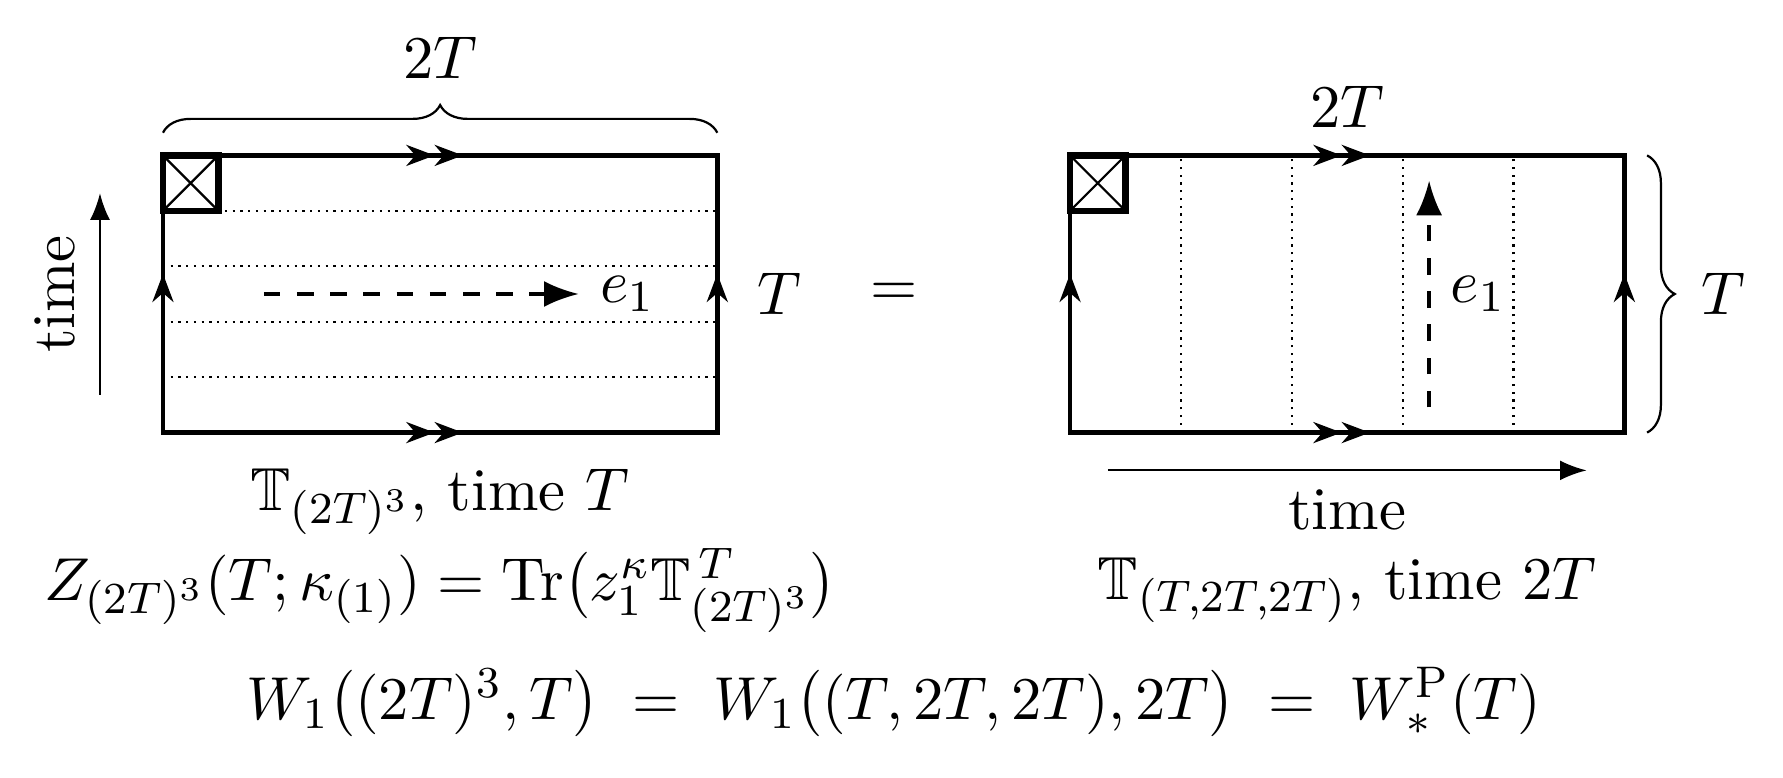
\includegraphics[width=320.8bp]{figures/fig10.png}
\caption{Rotation identity (\cref{thm:residue-split}\textup{(d),(f)}): the torus $\cube T\times T$ projected onto its first and fourth directions, with the two other directions suppressed; arrows mark the periodic identifications. The marked plaquette belongs to the stack $\Sigma_{14}$ that carries the twist $\kappa$. Left: time along the side $T$; Fourier transformation in $\kappa$ measures the electric flux $e_1$ along the side $2T$. Right: the same integral with direction $1$ as time, on the crossed box $(T,2T,2T)$ at time $2T$; the same Fourier transformation now measures the flux through the circle of length $T$. \Cref{thm:magnetic-P,thm:flux-count} read this integral once more, with direction $2$ as time.}
\label{fig:rotation}
\end{figure}

Part (g) restates \Bcirc{} through the two residues, with the tolerances $2^{-14}$ and $1/49155$ changed to $2^{-13}$; it proves neither \hypN{} nor \hypP. Since \Bcirc{} is the hypothesis of \cref{thm:ascent} and the proof of \cref{thm:main} uses \Mcirc{} only through \Bcirc{} (\cref{lem:purity-conversion}), the conclusions of \cref{thm:main} also hold with \Mcirc{} along the tuning replaced by \hypN{} and \hypP{} along the tuning. For $\SU(2)$ on a fixed lattice the flux residue tends to its ceiling $3\log2$ as $\beta\to\infty$ (\cref{prop:flux-saturation}), whereas (g) needs it below $2^{-13}$; so $T_0$ has to grow with $\beta$.

\subsection{Projected traces}

The split of \cref{thm:residue-split}\textup{(a)} uses only a finite group of symmetries of the transfer matrix that fixes the ground state.

\begin{theorem}[projected split]\label{thm:projected-split}
Let $\TT\ne0$ be a self-adjoint Hilbert--Schmidt operator $\TT\ge0$ on $L^2(X,\mu)$, $\mu$ $\sigma$-finite, with a kernel $\TT(x,y)\ge0$ and a simple largest eigenvalue $\lzero=\norm{\TT}$ whose unit eigenvector $\Omegazero$ is strictly positive outside a null set. Let $H$ be a finite group of operators $Uh=h\circ\sigma_U$ commuting with $\TT$, where $\sigma_U$ is a bijection of $X$ such that $\sigma_U$ and $\sigma_U^{-1}$ preserve $\mu$. For $T\ge2$ put $R=\TT/\lzero$, $\Zc=\Tr R^T$, $Z=\Tr\TT^T$, $Z_U=\Tr(U\TT^T)$, $P_H=\abs{H}^{-1}\sum_{U\in H}U$ and $Z_H=\Tr(P_H\TT^T)$.
\begin{enumerate}[label=\textup{(\roman*)},leftmargin=*]
\item $P_H$ is the orthogonal projection onto the $H$-invariant vectors, and $0\le Z_U\le Z$ for $U\in H$.
\item $Z/\abs{H}\le Z_H\le Z$.
\item $P_H\Omegazero=\Omegazero$.
\item $\Zc=\Tr(P_HR^T)\cdot Z/Z_H$, where $\Tr(P_HR^T)\ge1$ and $1\le Z/Z_H\le\abs{H}$.
\item The bound $\abs{H}$ cannot be improved: for $X=H$ with counting measure, $(U_gh)(x)=h(g^{-1}x)$, and $\TT_\varepsilon=(1-\varepsilon)1+\varepsilon J$ with $0<\varepsilon\le1$ and $J$ the orthogonal projection onto the constants, $Z/Z_H=1+(\abs{H}-1)(1-\varepsilon)^T$, which tends to $\abs{H}$ as $\varepsilon\to0$.
\end{enumerate}
\end{theorem}

\begin{proof}
(i) $H$ is a group of unitaries, so $UP_H=P_H$ for $U\in H$ and $P_H^*=P_H=P_H^2$. The kernel of $U\TT$ is $\TT(\sigma_Ux,y)\ge0$ and the kernel $t_{T-1}$ of $\TT^{T-1}$ is nonnegative, so $Z_U=\Tr\bigl((U\TT)\TT^{T-1}\bigr)=\iint\TT(\sigma_Ux,y)\,t_{T-1}(y,x)\dd\mu(y)\dd\mu(x)\ge0$. In an orthonormal eigenbasis $(\phi_i)$ of $\TT$ with eigenvalues $\lambda_i$, $Z_U=\sum_i\lambda_i^T\ip{\phi_i}{U\phi_i}$ and $\abs{\ip{\phi_i}{U\phi_i}}\le1$, so $Z_U\le Z$.

(ii) $Z_H=\abs{H}^{-1}\sum_UZ_U$, the term $U=1$ equals $Z$ and the others lie in $[0,Z]$.

(iii) $U\Omegazero=\Omegazero\circ\sigma_U$ is a unit eigenvector for $\lzero$, strictly positive outside a null set. By simplicity $U\Omegazero=c\,\Omegazero$ with $\abs{c}=1$ and $c=\ip{\Omegazero}{U\Omegazero}>0$, so $c=1$.

(iv) $\Tr(P_HR^T)=Z_H/\lzero^T$ and $\Zc=Z/\lzero^T$. By (iii), $\Tr(P_HR^T)=\Tr(P_HR^TP_H)\ge\ip{\Omegazero}{R^T\Omegazero}=1$, and the bounds on $Z/Z_H$ are (ii).

(v) $\TT_\varepsilon$ has the kernel $(1-\varepsilon)\delta_{xy}+\varepsilon/\abs{H}\ge0$ and commutes with every $U_g$. Its eigenvalues are $1$ on the constants, simple since $\varepsilon>0$, with a positive eigenvector, and $1-\varepsilon$ with multiplicity $\abs{H}-1$; so $Z=1+(\abs{H}-1)(1-\varepsilon)^T$. The left regular action is transitive, so the invariant functions are the constants, $P_H=J$ and $Z_H=1$.
\end{proof}

With $1-\varepsilon=\rho^{\Vol{s}}$, $\TT_\varepsilon$ realises on $L^2(H)$ the transfer matrix of the \PSTS{} $Z(n)=1+(\abs{H}-1)\rho^{|n|}$ of the proof of \cref{lem:E1-E3}. For every $f\in\Fclass(G)$ the hypotheses hold, by \cref{prop:class-weight-psts}, for the centre operators $z^k$, composition operators by the Haar-preserving maps $\zeta^k$, for which $P_H=P_0$ and $Z/Z_H=e^{\varphi}$, so that (iv) is \cref{thm:residue-split}\textup{(a)}; and for the spatial translations of $\Lambda_s$, which commute with $\TT_s$ because \eqref{eq:cg-kernel} is translation invariant, and for which $P_H$ projects onto the states of zero momentum. In the centre case on the cube of the datum put
\begin{equation}\label{eq:cg-ab}
a=\log\Tr\bigl(P_0R_{\cube{T_0}}^{T_0}\bigr),\qquad b=-\log(1-W),\qquad W=\sum_{e\ne0}w_e(\cube{T_0},T_0).
\end{equation}
Then $a,b\ge0$, $b=\varphi_{\cube{T_0}}(T_0)$ and $\XT{\cube{T_0}}{T_0}=a+b$, so \Bcirc{} holds at $T_0$ if and only if $a+b\le\xconstinl$, and \Mcirc{} at $T_0$ implies $a+b\le\xconstinl$.

On the window of the first paper the same split gives a necessary and a sufficient condition for the rational condition \eqref{ms:eq:rational-condition}; we state it for $\SU(2)$.

\begin{proposition}[window split]\label{prop:window-split}
Let $G=\SU(2)$, $C=\{\pm1\}$, $T_0\ge3$ and $s\in\Wwin_{T_0}$. Write $\psi=\psiT{s}{T_0}$, $\psi^0=\psi^0_s(T_0)$, $W=1-w_0(s,T_0)$ and $x=\Vol{s}/(161(48T_0)^3)$. Then $x<1/161$, and:
\begin{enumerate}[label=\textup{(\alph*)},leftmargin=*]
\item if $\psi^0\le\Vol{s}/(322(48T_0)^3)$ and $W\le\Vol{s}/(645(48T_0)^3)$, then $\psi\le x$;
\item if $\psi\le x$, then $W\le x$ and $\psi^0\le2x$.
\end{enumerate}
Consequently the two conditions of \textup{(a)} for every $s\in\Wwin_{T_0}$ imply \eqref{ms:eq:rational-condition}, and \eqref{ms:eq:rational-condition} implies $W\le x$ and $\psi^0\le2x$ for every $s\in\Wwin_{T_0}$.
\end{proposition}

\begin{proof}
$x<1/161$ because $s_j<48T_0$. (a) The hypotheses read $\psi^0\le x/2$ and $W\le161x/645<1/645$. Hence $\varphi=-\log(1-W)\le W/(1-W)\le\frac{161x}{645}\cdot\frac{645}{644}=\frac x4$, and \cref{thm:residue-split}\textup{(c)} gives $\psi\le2\varphi+\psi^0\le x$. (b) By \cref{thm:residue-split}\textup{(c)}, $\varphi\le\psi\le x$, so $W=1-e^{-\varphi}\le x$. The largest eigenvalue of $R_s$ on $\Kspace^0_s$ is $1$, with eigenvector $\Omegazero$, so the argument of (E3) on $\Kspace^0_s$ gives $\psi^0\le2\log\Zc^0_s(T_0)$. By \cref{thm:residue-split}\textup{(a)} and \eqref{eq:X-psi}, $\log\Zc^0_s(T_0)\le\XT{s}{T_0}\le\psi$; so $\psi^0\le2\psi\le2x$.
\end{proof}

\subsection{What the two residues do not control}

\begin{proposition}[the residues are independent]\label{prop:no-residue-control}
\begin{enumerate}[label=\textup{(\alph*)},leftmargin=*]
\item Let $Z_A$ be the system of this section and $Z_B$ a \PSTS{} with transfer matrices $\TT^B_s$. Then $Z=Z_AZ_B$ is a \PSTS{} with $\TT_s=\TT^A_s\otimes\TT^B_s$, centre operators $z^k\otimes1$ and projections $P_e\otimes1$. Its twisted ratios $Z_s(T;k)/\Zpart{s}{T}$, hence $w_e$, $\varphi$, $W_j$ and $W^{\mathrm P}_*$, are those of $Z_A$, while $\Zc^0_s(T)=\Zc^{0,A}_s(T)\,\Zs{s}{T}^B$. For $f\equiv1$ \textup{(}Wilson theory at $\beta=0$\textup{)} and $Z_B(n)=1+q\,a^{|n|}$ with an integer $q\ge1$ and $0<a<1$, $W^{\mathrm P}_*(T)=0$ and $\log\Zc^0_{\cube T}(T)=\log(1+q\,a^{8T^4})$: \hypP{} holds at every $T$, \hypN{} fails at $T$ when $q\,a^{8T^4}>e^{2^{-14}}-1$, and no finite-valued function $g$ satisfies $\log\Zc^0_{\cube T}(T)\le g(W^{\mathrm P}_*(T))$ for all these systems.
\item Let $G=C=\{\pm1\}\subset\U(1)$ and $f(g)=e^{\beta g}$, the Wilson weight with $N_c=1$. For fixed $s$ and $T\ge3$, as $\beta\to\infty$: $\log\Zc^0_s(T)\to0$, $w_e(s,T)\to1/8$ for every $e$, $\varphi_s(T)\to\log8$ and $W_j(s,T)\to1/2$; in particular $W^{\mathrm P}_*(T)\to1/2$. There is no function $g$ continuous at $0$ with $g(0)=0$ such that $W^{\mathrm P}_*(T)\le g(\log\Zc^0_{\cube T}(T))$ for all systems of this section.
\end{enumerate}
\end{proposition}

\begin{proof}
(a) $\Tr\bigl((z^k\otimes1)(\TT^A_s\otimes\TT^B_s)^T\bigr)=Z^A_s(T;k)\,\Zpart{s}{T}_B$, so the ratios are those of $Z_A$, and $w_e$, $\varphi$, $W_j$, $W^{\mathrm P}_*$ are functions of the ratios by \eqref{eq:cg-duality} and \eqref{eq:cg-Wj}. With $R_s=R^A_s\otimes R^B_s$, $\Tr\bigl((P_0\otimes1)R_s^T\bigr)=\Tr(P_0(R^A_s)^T)\Tr((R^B_s)^T)$. For $f\equiv1$ every integral \eqref{eq:cg-twisted} equals $1$, so all ratios are $1$, $w_0=1$ and $W_j=0$, and $\TT^A_s$ is the projection onto the constants, so $\Zc^{0,A}=1$. The proof of \cref{lem:E1-E3} gives $\TT^B_s=\mathrm{diag}(1,a^{\Vol{s}},\dots,a^{\Vol{s}})$ and $\Zs{\cube T}{T}^B=1+q\,a^{8T^4}$, which is unbounded in $q$.

(b) Let $V=\Vol{s}$. The exponent in \eqref{eq:cg-kernel} is at most $6\beta V$, with equality exactly when $Q$ and $Q'$ are flat (all spatial plaquette variables equal $1$) and $Q'=U\cdot Q$; so $e^{-6\beta V}\TT_s\to F$ with $(Fh)(Q)=2^{-4V}\mathbf 1[Q\text{ flat}]\sum_Uh(U\cdot Q)$. On the connected torus $\Lambda_s$ the stabiliser of a configuration in the gauge group is $\{\pm1\}$, so all gauge orbits have $2^{V-1}$ elements, and $F$ is a positive multiple of the orthogonal projection $E$ onto the span of the indicator functions of the orbits of flat configurations. These $8$ orbits are labelled by the holonomies $h\in\{\pm1\}^3$ along the coordinate cycles; $z_j^{-1}$ multiplies the holonomy along cycle $j$ by $-1$, as that cycle contains exactly one $j$-link with $x_j=0$, and fixes the two others. So the $z^k$ act on the range of $E$ by the regular representation of $C^3$, and $\Tr(P_eE)=1$ for every $e$. As $\Kspace_s$ is finite-dimensional, $e^{-6\beta V}\lzero(s)$ tends to the nonzero eigenvalue of $F$, $R_s\to E$ and $\Tr(P_eR_s^T)\to1$. Hence $\Zc\to8$, $\Zc^0\to1$, $w_e\to1/8$, $\varphi\to\log8$ and $W_j\to1/2$. The case $s=s_\times(T)$ at time $2T$ gives $W^{\mathrm P}_*(T)\to\frac12$, and comparison with $s=\cube T$ at time $T$ gives the last claim.
\end{proof}

Both examples have positive transfer matrices and the centre grading of \cref{lem:centre-operators}. \Cref{prop:no-residue-control} says nothing about pure $\SU(N_c)$ theory; it shows that a bound of one residue by the other must use properties that these examples lack.

For a centre of scalars the flux residue bounds Polyakov loop correlators. On the torus $(s,T)$ let $L_y=U_{((y,0),4)}U_{((y,1),4)}\cdots U_{((y,T-1),4)}$ be the Polyakov loop at $y\in\Lambda_s$ and, for $j\in\{1,2,3\}$ and $0<r<s_j$,
\[
\Phi(r)=\Zpart{s}{T}^{-1}\int\overline{\Tr L_y}\,\Tr L_{y+re_j}\prod_pf(Q_p)\prod_{(x,\mu)}\dd U_{(x,\mu)},
\]
which does not depend on $y$. Put $\theta=r/s_j$, $u_a=\sum_{e:\,e_j=a}w_e(s,T)$ for $a\in\widehat C$, and $W=W_j(s,T)=\sum_{a\ne0}u_a$.

\begin{proposition}[Polyakov loops]\label{prop:polyakov-bound}
Suppose that every $c\in C$ is a scalar matrix, $c=\chi(c)1$, and $C\ne\{1\}$.
\begin{enumerate}[label=\textup{(\alph*)},leftmargin=*]
\item $0\le\Phi(r)\le N_c^2\sum_{a\in\widehat C}u_a^{1-\theta}u_{a+\chi}^{\theta}\le N_c^2\bigl(W^\theta+W^{1-\theta}+W\bigr)$.
\item If \Bcirc{} holds at $T_0$, in particular if \Mcirc{} holds at $T_0$, then on $\cube{T_0}\times T_0$
\[
\Phi(T_0)\le N_c^2\Bigl(\frac2{\sqrt{8192}}+\frac1{8192}\Bigr)<0.0223\,N_c^2 .
\]
\item The bound \textup{(a)} has no converse: for $G=C=\{\pm1,\pm i\}\subset\U(1)$ and $f(g)=\exp(\beta\operatorname{Re}g^2)$, $\beta\ge0$, one has $f\in\Fclass(G)$, $\Phi(r)=0$ for $0<r<s_j$, and $W_j(s,T)\ge\frac12-2^{4|n|-1}e^{-2\beta}$ with $|n|=\Vol{s}T$. So $W^{\mathrm P}_*\to\frac12$ as $\beta\to\infty$, while every correlator of fundamental Polyakov loops vanishes.
\end{enumerate}
\end{proposition}

\begin{proof}
(a) Read the torus with axis $j$ as time: let $\TT'$ be the transfer matrix of the torus $s^{(j)}$ of \cref{thm:residue-split}\textup{(d)}, $R'=\TT'/\lzero(s^{(j)})$ and $M'=s_j$. Then $L_y$ and $L_{y+re_j}$ lie in the time slices $0$ and $r$, as products of the $T$ links of a line in the new direction $j$. With $A$ the multiplication by the trace of this product, the iterated-kernel computation of \cref{lem:transfer-matrix}\textup{(iii)} with two insertions gives $\Phi(r)=\Tr(A^*R'^rAR'^{M'-r})/\Tr R'^{M'}$. As $R'$ is Hilbert--Schmidt and $M'\ge3$, $B=R'^{r/2}AR'^{(M'-r)/2}$ is Hilbert--Schmidt, and $\Tr(A^*R'^rAR'^{M'-r})=\norm{B}_2^2\ge0$ by cyclicity.

Let $z'^c_j$ be the centre operator of the new direction $j$ and $P'_a=\abs{C}^{-1}\sum_c\overline{a(c)}z'^c_j$, $a\in\widehat C$. The line contains exactly one link moved by $z'^c_j$, so $z'^c_jA=\chi(c)Az'^c_j$, hence $AP'_a=P'_{a+\chi}A$; the $P'_a$ are orthogonal projections commuting with $R'$, with $\sum_aP'_a=1$. By the proof of \cref{thm:residue-split}\textup{(d)} and \cref{lem:centre-operators}\textup{(c)}, $Z_{s^{(j)}}(s_j;\kappa_{(j)})=Z_s(T;\kappa_{(j)})$, so \eqref{eq:cg-duality} gives $\Tr(P'_aR'^{M'})/\Tr R'^{M'}=\abs{C}^{-1}\sum_\kappa\overline{a(\kappa)}Z_s(T;\kappa_{(j)})/\Zpart{s}{T}=u_a$. Now $B=\sum_aB_a$ with $B_a=P'_{a+\chi}R'^{r/2}AR'^{(M'-r)/2}P'_a$, and $B_a^*B_b=0$ for $a\ne b$, so $\norm{B}_2^2=\sum_a\norm{B_a}_2^2$. H\"older's inequality for Schatten norms with exponents $2M'/r$ and $2M'/(M'-r)$, and $\norm{A}\le N_c$, give
\[
\norm{B_a}_2^2\le N_c^2\bigl(\Tr P'_{a+\chi}R'^{M'}\bigr)^{\theta}\bigl(\Tr P'_aR'^{M'}\bigr)^{1-\theta},
\]
and division by $\Tr R'^{M'}$ gives the first bound. The character $\chi$ is injective, hence nonzero. The term $a=0$ is at most $u_\chi^\theta\le W^\theta$, the term $a=-\chi$ is at most $u_{-\chi}^{1-\theta}\le W^{1-\theta}$, and by Young's inequality the sum of the remaining terms is at most $\sum_{a\ne0,-\chi}(\theta u_{a+\chi}+(1-\theta)u_a)\le W$.

(b) By \cref{thm:residue-split}\textup{(f),(g)}, $W=W^{\mathrm P}_*(T_0)<2^{-13}$, and $\theta=T_0/(2T_0)=\frac12$; so (a) gives $\Phi(T_0)\le N_c^2(2W^{1/2}+W)$.

(c) $f(\pm1)=e^\beta$ and $f(\pm i)=e^{-\beta}$, so $f_0=\cosh\beta$, $f_2=\sinh\beta$ and $f_1=f_3=0$ for the characters $g\mapsto g^m$; thus $f\in\Fclass(G)$. As $(-Q)^2=Q^2$, multiplying the link $((y,0),4)$ by $-1$ preserves the weight and Haar measure, changes $L_y$ to $-L_y$ and leaves $L_{y+re_j}$ unchanged; so $\Phi(r)=-\Phi(r)=0$. Next, $f(\eta_pQ_p)=\exp(\beta\operatorname{Re}(\eta_p^2Q_p^2))$, $Q_p^2$ is the plaquette variable of $V=(U_\ell^2)_\ell\in\{\pm1\}^{\text{links}}$, and $U\mapsto U^2$ maps Haar measure onto Haar measure. So $Z_s(T;i_{(j)})=\int\prod_p\exp(\beta\varepsilon_pV_p)\dd V$ with $\varepsilon_p=-1$ on the stack and $1$ elsewhere, and $\Zpart{s}{T}$ is the same integral with $\varepsilon\equiv1$, which is at least $e^{6\beta|n|}2^{-4|n|}$, the configuration $V\equiv1$ having Haar measure $2^{-4|n|}$. Each $(j,4)$-plane two-torus contains one plaquette of the stack, and the product of $V_p$ over its plaquettes is $1$, every link lying on two of them; so $\varepsilon_pV_p=-1$ for some plaquette of it, $\sum_p\varepsilon_pV_p\le6|n|-2$, and $\alpha=Z_s(T;i_{(j)})/\Zpart{s}{T}\le2^{4|n|}e^{-2\beta}$. Also $Z_s(T;(-1)_{(j)})=\Zpart{s}{T}$ and $Z_s(T;(-i)_{(j)})=Z_s(T;i_{(j)})$. With the characters $a(\kappa)=\kappa^a$, \eqref{eq:cg-duality} gives $u_a=\frac14\bigl(1+(-1)^a+\alpha(i^{-a}+(-i)^{-a})\bigr)$, so $u_1=u_3=0$, $u_2=(1-\alpha)/2$ and $W_j=u_2\ge\frac12-2^{4|n|-1}e^{-2\beta}$.
\end{proof}

\subsection{The flux residue on the crossed box}

Fix $T_0\ge3$ and write $X_0=\XT{\cube{T_0}}{T_0}$, $s_\times=s_\times(T_0)=(T_0,2T_0,2T_0)$, $R_\times=R_{s_\times}$, $X'=\log\Tr R_\times^{2T_0}=\XT{s_\times}{2T_0}$ and $P_{\ne}=\sum_{e:\,e_1\ne0}P_e$ on $\Kspace_{s_\times}$, so that $W^{\mathrm P}_*=W^{\mathrm P}_*(T_0)=\Tr(P_{\ne}R_\times^{2T_0})/\Tr R_\times^{2T_0}$. Let $\zeta$ be the function of \cref{lem:exchange} for $b=c=2T_0$. Part (c) of that lemma with $T=T_0$ reads
\begin{equation}\label{eq:cg-crossed}
X_0=X'+T_0\delta,\qquad \delta=2\zeta(T_0)-\zeta(2T_0)\in[\zeta(T_0),2\zeta(T_0)],\qquad\text{hence }0\le X'\le X_0 .
\end{equation}
For $\kappa\in C$ let $\TT_\kappa$ be the operator of \cref{lem:centre-operators}\textup{(d)} for $s=s_\times$, $T=2T_0$, $j=1$ and $i=2$. As $s_2=2T_0$, $s^{(2)}=s_\times$, and $\TT_\kappa$ is $\TT_{s_\times}$ with the twist $\kappa$ on the $(1,2)$-plaquettes at $x_1=x_2=0$, a magnetic flux $\kappa$ through the $(1,2)$-planes. Let $\lambda_{0,\kappa}=\norm{\TT_\kappa}$, $D_\kappa(M)=\Tr(\TT_\kappa/\lambda_{0,\kappa})^M-1\ge0$, and
\[
\tau_\kappa=\log\frac{\lzero(s_\times)}{\lambda_{0,\kappa}},\quad \rho_\kappa=\frac{1+D_\kappa(2T_0)}{\Zs{s_\times}{2T_0}},\quad v_\kappa=1-\frac{Z_{s_\times}(2T_0;\kappa_{(1)})}{\Zpart{s_\times}{2T_0}},\quad F_v(\kappa)=-\log(1-v_\kappa),
\]
the magnetic flux energy per unit length, the excess ratio, the vortex weight and the vortex free energy.

\begin{theorem}[magnetic form of the flux condition]\label{thm:magnetic-P}
Let $T_0\ge3$ and $\kappa\in C$.
\begin{enumerate}[label=\textup{(\alph*)},leftmargin=*]
\item $1-v_\kappa=e^{-2T_0\tau_\kappa}\rho_\kappa$, so $F_v(\kappa)=2T_0\tau_\kappa-\log\rho_\kappa\ge0$; moreover $\tau_\kappa\ge0$ and $\rho_\kappa\ge e^{-X'}$.
\item $v_\kappa\le1-e^{-2T_0\tau_\kappa-X'}\le2T_0\tau_\kappa+X'\le2T_0\tau_\kappa+X_0-T_0\,\zeta(T_0)$.
\item $v_\kappa\le2W^{\mathrm P}_*$. If \hypP{} holds at $T_0$, then $v_\kappa\le2/49155$, $F_v(\kappa)\le2/49153$ and $2T_0\tau_\kappa\le\log(1+D_\kappa(2T_0))-X'+2/49153$.
\end{enumerate}
\end{theorem}

\begin{proof}
(a) By \cref{lem:centre-operators}\textup{(d)}, $Z_{s_\times}(2T_0;\kappa_{(1)})=\Tr\TT_\kappa^{2T_0}=\lambda_{0,\kappa}^{2T_0}(1+D_\kappa(2T_0))$, and $\Zpart{s_\times}{2T_0}=\lzero(s_\times)^{2T_0}e^{X'}$; dividing gives the identity. $\tau_\kappa\ge0$ by \cref{lem:centre-operators}\textup{(d)}, $\rho_\kappa\ge e^{-X'}$ as $D_\kappa\ge0$, and $F_v\ge0$ as $0<Z_{s_\times}(2T_0;\kappa_{(1)})\le\Zpart{s_\times}{2T_0}$. (b) By (a), $v_\kappa\le1-e^{-2T_0\tau_\kappa-X'}$; then use $1-e^{-y}\le y$ and \eqref{eq:cg-crossed}. (c) By \eqref{eq:cg-duality}, $1-v_\kappa=\sum_ee_1(\kappa)w_e$, which is real, so $v_\kappa=\sum_e(1-\operatorname{Re}e_1(\kappa))w_e\le2\sum_{e_1\ne0}w_e=2W^{\mathrm P}_*$. Under \hypP, $v_\kappa\le2/49155$ and $F_v\le\log\frac{49155}{49153}\le\frac2{49153}$, and $2T_0\tau_\kappa=\log\rho_\kappa+F_v=\log(1+D_\kappa(2T_0))-X'+F_v$.
\end{proof}

\begin{remark}
\hypP{} at $T_0$ already follows from $X'\le-\log(1-1/49155)$, in particular from $X_0\le1/49155$, because $W^{\mathrm P}_*\le1-e^{-X'}$ by \cref{thm:flux-count}\textup{(a)}. No bound on $\tau_\kappa$ is needed for this; part (c) is a necessary condition on the magnetic flux energy.
\end{remark}

The flux weight is also controlled by the spectrum of $R_\times$ on the sectors with $e_1\ne0$, the electric-flux states of the crossed box. Let $r_{\ne}=\norm{P_{\ne}R_\times}$, so that $-\log r_{\ne}$ is the lowest energy of a state with nonzero electric flux in direction $1$, and $\mathcal N_m=\Tr(P_{\ne}R_\times^m)$ for $2\le m\le2T_0$, a weighted count of these states. Part (b) of the next theorem is a conditional theorem. Its hypothesis, the Hamiltonian area law $r_{\ne}\le e^{-\sigma T_0}$ together with the count condition $\sigma T_0^2\ge\log49155+\log\mathcal N_{T_0}$, is not proved here; it is not weaker than \Mcirc{} in any sense proved here.

\begin{theorem}[flux count]\label{thm:flux-count}
Let $T_0\ge3$ and $2\le m\le2T_0$.
\begin{enumerate}[label=\textup{(\alph*)},leftmargin=*]
\item $W^{\mathrm P}_*\le\Tr(P_{\ne}R_\times^{2T_0})\le\mathcal N_m\,r_{\ne}^{2T_0-m}$, $\mathcal N_m\le\Zs{s_\times}{m}-1$, and $W^{\mathrm P}_*\le1-e^{-X'}\le X'$.
\item If $r_{\ne}\le e^{-\sigma T_0}$ with $\sigma\ge0$, then $W^{\mathrm P}_*\le\mathcal N_me^{-\sigma T_0(2T_0-m)}$, and \hypP{} holds at $T_0$ if $\sigma T_0^2\ge\log49155+\log\mathcal N_{T_0}$, where $\log49155\in(10.80,10.81)$ and $\mathcal N_{T_0}\le\Zs{s_\times}{T_0}-1$.
\item $r_{\ne}^{2T_0}\le W^{\mathrm P}_*e^{X'}$. If \hypP{} holds at $T_0$, then $-\log r_{\ne}\ge(\log49155-X')/(2T_0)>(10.80-X')/(2T_0)$.
\end{enumerate}
\end{theorem}

\begin{proof}
(a) $\Tr R_\times^{2T_0}\ge1$ gives the first inequality. $A=P_{\ne}R_\times\ge0$, since $P_{\ne}$ is a projection commuting with $R_\times$, and $\Tr(P_{\ne}R_\times^{2T_0})=\Tr(A^mA^{2T_0-m})\le\norm{A}^{2T_0-m}\Tr A^m$. Since $\Omegazero\in\Kspace^0$ and $P_0\le1-P_{\ne}$, $P_{\ne}\le1-\ip{\Omegazero}{\cdot\,}\Omegazero$, so $\mathcal N_m\le\Tr R_\times^m-1$. At $m=2T_0$ this gives $W^{\mathrm P}_*\le(\Tr R_\times^{2T_0}-1)/\Tr R_\times^{2T_0}=1-e^{-X'}\le X'$. (b) Insert $r_{\ne}\le e^{-\sigma T_0}$ in (a) and take $m=T_0$. (c) $r_{\ne}^{2T_0}=\norm{A}^{2T_0}\le\Tr A^{2T_0}=W^{\mathrm P}_*\Tr R_\times^{2T_0}=W^{\mathrm P}_*e^{X'}$; under \hypP{} take logarithms.
\end{proof}

\begin{remark}
Part (c) gives only $-\log r_{\ne}\ge(10.80-X')/(2T_0)$, a bound of order $1/T_0$, whereas the hypothesis of (b) is $-\log r_{\ne}\ge\sigma T_0$. At the threshold value of $\sigma$ in (b), the two conditions on $-\log r_{\ne}$ are $(\log49155+\log\mathcal N_{T_0})/T_0$ and $(\log49155-X')/(2T_0)$; they differ by the count $\mathcal N_{T_0}$ and a factor $2$.
\end{remark}

\subsection{The neutral residue}

\begin{corollary}[neutral threshold]\label{cor:neutral-threshold}
Suppose that \hypN{} holds at $T_0$, and let $e^{-E}$ be an eigenvalue of $R_{\cube{T_0}}$ on $\Kspace^0_{\cube{T_0}}\ominus\C\Omegazero$. Then
\[
T_0E\ge-\log\bigl(e^{2^{-14}}-1\bigr)\in(9.70403,\,9.70404),
\]
in particular $T_0E>9.7040$. For every $x>0$ at most $(e^{2^{-14}}-1)e^x$ of these eigenvalues, counted with multiplicity, satisfy $T_0E\le x$.
\end{corollary}

\begin{proof}
$R=R_{\cube{T_0}}$ commutes with $P_0$ and $\Omegazero\in\Kspace^0$, so $\Zc^0_{\cube{T_0}}(T_0)=1+\sum_ie^{-T_0E_i}$, the sum over the eigenvalues $e^{-E_i}$ of $R$ on $\Kspace^0\ominus\C\Omegazero$ with multiplicity. By \hypN, $\sum_ie^{-T_0E_i}\le e^{2^{-14}}-1$; each term is at most this sum, and the number of terms with $T_0E_i\le x$ is at most $e^x\sum_ie^{-T_0E_i}$.
\end{proof}

Under \Bcirc{} at $T_0$, \cref{prop:spectral-conditions} gives $T_0(E_1-E_0)\ge13\log2-2^{-13}>9.0107$ for all excitations; \hypN{} is a condition on the neutral sector alone and forces the larger threshold $9.7040$ there.

\subsection{The rate form of the datum}

The datum compares two partition functions on one cube. Along a family it is equivalent to three statements about quantities that are uniform in the volume: a gap of the centre-neutral sector, a decay rate of 't Hooft's vortex weight, and a bound on the neutral thermal free energy, all in physical units. Each of the three is independent of the other two among centre-graded \PSTS{} (\cref{prop:criterion-independence}), and none is proved at weak coupling along the continuum tuning.

Let $(Z_{N,p})$ be a family of \PSTS{} as in \cref{thm:zero-one}, write $r_1^{N,p}(s)$ for $r_1(s)$ computed in $Z_{N,p}$, and put, with $-\log0=+\infty$,
\[
\mathsf m(t)=\liminf_{p\to\infty}\,\liminf_{N\to\infty}\,N\bigl(-\log r_1^{N,p}(\cube{\lfloor Nt\rfloor})\bigr)\in[0,\infty],\qquad \mathsf m_\infty=\liminf_{t\to\infty}\mathsf m(t),
\]
the spectral gap of the cube of physical side $2t$, measured along the family in physical units. We use $e^{-\infty}=0$.

\begin{theorem}[gapped transport]\label{thm:gapped-transport}
Let $Z$ be a \PSTS{} and $T'\ge T\ge3$ integers. Then
\begin{equation}\label{eq:transport}
X(T')\le r_1\bigl(\cube{T'}\bigr)^{T'-T}\Bigl(\exp\Bigl(8\bigl(\tfrac{T'}{T}\bigr)^3X(T)\Bigr)-1\Bigr).
\end{equation}
\end{theorem}

\begin{proof}
Let $s=\cube{T'}$. Its sides are $2T'\ge2T$, so \eqref{eq:cube-control} gives $\log\Zs{s}{T}\le8(T'/T)^3X(T)$, that is $\Dexc{s}{T}\le\exp(8(T'/T)^3X(T))-1$. The second bound of \eqref{eq:gap-step} with $M=T'\ge M'=T\ge2$ gives $\Dexc{s}{T'}\le r_1(s)^{T'-T}\Dexc{s}{T}$, and $X(T')=\log(1+\Dexc{s}{T'})\le\Dexc{s}{T'}$.
\end{proof}

At $T'=2T$ the bound \eqref{eq:transport} replaces one factor $\Dexc{s}{T}$ of the one-step bound $X(2T)\le\Dexc{s}{T}^2$ of \eqref{eq:one-step} by $r_1(s)^T$.

\begin{theorem}[two-number criterion]\label{thm:two-number}
Let $(Z_{N,p})$ be a family as in \cref{thm:zero-one}, and $0<t_1<t_2$ with $y(t_1)<\infty$. Then
\begin{equation}\label{eq:two-number}
y(t_2)\le e^{-(t_2-t_1)\mathsf m(t_2)}\Bigl(e^{8(t_2/t_1)^3y(t_1)}-1\Bigr).
\end{equation}
\Mcirc{} holds along the family if and only if there are $0<t_1<t_2$ with $y(t_1)<\infty$ and right side of \eqref{eq:two-number} less than $1/8194$; in that case \Mcirc{} holds along the family with $\tzero=t_2$. If the right side is less than some $c\in(0,x_c)$, then \Bcirc{} holds along the family with $\tzero=2^{i_0(c)}t_2$ and \Mcirc{} with $\tzero=2^{i_0(c)+3}t_2$, where $i_0(c)$ is the integer of \cref{thm:zero-one}\textup{(b)}.
\end{theorem}

\begin{proof}
Fix $p$ with $Y_p(t_1):=\limsup_NX_{N,p}(\lfloor Nt_1\rfloor)<\infty$; since $y(t_1)<\infty$, this holds for all large $p$. For large $N$ the integers $T=\lfloor Nt_1\rfloor$ and $T'=\lfloor Nt_2\rfloor$ satisfy $T'\ge T\ge3$. Put $a_N=N(-\log r_1^{N,p}(\cube{T'}))\in[0,\infty]$, $b_N=(T'-T)/N$ and $c_N=8(T'/T)^3$, so that $b_N\to t_2-t_1>0$ and $c_N\to8(t_2/t_1)^3$. By \cref{thm:gapped-transport},
\[
X_{N,p}(T')\le e^{-b_Na_N}\bigl(e^{c_NX_{N,p}(T)}-1\bigr).
\]
Both factors are nonnegative, the first is at most $1$, and the second has finite limit superior $\le e^{8(t_2/t_1)^3Y_p(t_1)}-1$. Since $b_N\to t_2-t_1>0$, $\liminf_Nb_Na_N=(t_2-t_1)\liminf_Na_N$, and $\limsup_Ne^{-b_Na_N}=e^{-(t_2-t_1)m_p}$ with $m_p=\liminf_Na_N$. The limit superior of a product of nonnegative sequences with finite limits superior is at most the product of these, so
\[
Y_p(t_2)\le e^{-(t_2-t_1)m_p}\bigl(e^{8(t_2/t_1)^3Y_p(t_1)}-1\bigr)
\]
for all large $p$. Taking $\limsup_p$ in the same way, with $\mathsf m(t_2)=\liminf_pm_p$ and $y(t_1)=\limsup_pY_p(t_1)<\infty$, gives \eqref{eq:two-number}.

If the right side of \eqref{eq:two-number} is less than $1/8194$, then $y(t_2)<1/8194$. As in the proof of \cref{thm:zero-one}\textup{(c)}, there is $p_0$ with $\limsup_NX_{N,p}(\lfloor Nt_2\rfloor)<1/8194$ for $p\ge p_0$, and then $N_0(p)$ with $X_{N,p}(\lfloor Nt_2\rfloor)<1/8194$ and $\lfloor Nt_2\rfloor\ge3$ for $N\ge N_0(p)$; by \eqref{eq:X-psi}, $T_0=\lfloor Nt_2\rfloor\le Nt_2$ has $\psiT{\cube{T_0}}{T_0}\le2X_{N,p}(T_0)<\dconstinl$. This is \Mcirc{} along the family with $\tzero=t_2$. If the right side is less than $c<x_c$, then $y(t_2)<c$, and the last step of the proof of \cref{thm:zero-one}\textup{(c)} gives \Bcirc{} along the family with $\tzero=2^{i_0(c)}t_2$; \cref{thm:upward-closed}\textup{(a)} turns \Bcirc{} at $T_0\le N\tzero$ into \Mcirc{} at $8T_0\le8N\tzero$.

Conversely, suppose \Mcirc{} along the family with $\tzero$, and let $\Delta=\tzero^{-1}\log\frac{63}{32}$. By \cref{lem:purity-conversion}, \Bcirc{} holds along the family with $\tzero$. Let $t>\tzero$. For all large $p$ and $N\ge\max\{N_0(p),1/(t-\tzero)\}$ there is $T_0\le N\tzero$ with $X_{N,p}(T_0)\le\xconstinl$, and $\lfloor Nt\rfloor\ge Nt-1\ge N\tzero\ge T_0$; \cref{thm:ascent}\textup{(b)} on the cube of side $n=2\lfloor Nt\rfloor\ge2T_0$ gives $N(-\log r_1^{N,p}(\cube{\lfloor Nt\rfloor}))\ge N\log\frac{63}{32}/T_0\ge\Delta$. Hence $\mathsf m(t)\ge\Delta$ for $t>\tzero$. By \cref{thm:zero-one}\textup{(c)}, $y(t)\le e^{-\Delta t/2}/64\le1$ for $t>\tzero$. With $t_2=2t_1$ and $t_1>\tzero$ the right side of \eqref{eq:two-number} is at most $e^{-\Delta t_1}(e^{64y(t_1)}-1)\le e^{-\Delta t_1}(e-1)$, because $64y(t_1)\le e^{-\Delta t_1/2}\le1$; it is less than $1/8194$ for large $t_1$.
\end{proof}

\begin{corollary}[gap and Stefan--Boltzmann bound]\label{cor:gap-sb}
For a family as in \cref{thm:zero-one} the following are equivalent:
\begin{enumerate}[label=\textup{(\roman*)},leftmargin=*]
\item \Mcirc{} along the family;
\item $\mathsf m_\infty>0$ and $\liminf_{t\to\infty}y(t)/t<\mathsf m_\infty/54$;
\item $\mathsf m_\infty>0$ and $\liminf_{t\to\infty}y(t)<\infty$.
\end{enumerate}
If $\mathsf m(t)\ge\Delta>0$ and $y(t)\le K<\infty$ for all $t\ge t_*$, then \Mcirc{} holds along the family with every $\tzero>\max\{\frac32t_*,(81K+3\log8194)/\Delta\}$.
\end{corollary}

\begin{proof}
(i)$\Rightarrow$(iii): by the proof of \cref{thm:two-number}, \Mcirc{} with $\tzero$ gives $\mathsf m(t)\ge\tzero^{-1}\log\frac{63}{32}$ for $t>\tzero$, and $y(t)\to0$ by \cref{thm:zero-one}\textup{(c)}. (iii)$\Rightarrow$(ii): if $y(t_n)\le K'$ along $t_n\to\infty$, then $y(t_n)/t_n\to0<\mathsf m_\infty/54$. (ii)$\Rightarrow$(i): choose $\ell$ and $g$ with $\liminf_ty(t)/t<\ell$ and $54\ell<g<\mathsf m_\infty$. There are arbitrarily large $t_1$ with $y(t_1)<\ell t_1$ and $\mathsf m(\frac32t_1)\ge g$. With $t_2=\frac32t_1$ the right side of \eqref{eq:two-number} is at most
\[
\exp\Bigl(8\cdot\tfrac{27}8\,y(t_1)-\tfrac12t_1\mathsf m(t_2)\Bigr)\le\exp\bigl(-\tfrac12t_1(g-54\ell)\bigr),
\]
which is less than $1/8194$ for large such $t_1$; \cref{thm:two-number} gives (i). For the last claim take $t_1>\max\{t_*,2(27K+\log8194)/\Delta\}$ and $t_2=\frac32t_1$: the right side of \eqref{eq:two-number} is at most $e^{27K-\Delta t_1/2}<1/8194$, and \cref{thm:two-number} gives \Mcirc{} with $\tzero=t_2$.
\end{proof}

The factor $54$ is $\min_{k>1}8k^3/(k-1)$, attained at $k=\frac32$; it is the best constant that \eqref{eq:two-number} gives with $t_2=kt_1$. The round trip loses a bounded factor: \Mcirc{} with $\tzero$ gives $\Delta=\tzero^{-1}\log\frac{63}{32}$ and, for $t_*\downarrow\tzero$, $K\le(32/63)^{1/2}/64<0.011136$ by \cref{thm:zero-one}\textup{(c)}, and the last part of \cref{cor:gap-sb} returns \Mcirc{} with every $\tzero'>41.24\,\tzero$.

A positive gap alone does not give \Mcirc{}: for the rings of \cref{prop:gapless-sector}\textup{(c)}, $\mathsf m\equiv\Delta$ and $y\equiv\infty$, and \cref{thm:hidden-sector}\textup{(d)} attaches them to any gauge theory without changing a single law of its links. By \cref{cor:gap-sb} the only further input needed is a bound on the thermal free energy of cubes of fixed physical size, of any size.

\begin{remark}[a level count suffices]\label{rem:sb-count}
Let $n_{N,p}(\varepsilon;t)$ be the number of eigenvalues $r_i$, $i\ge1$, of $R_{\cube{\lfloor Nt\rfloor}}$ in $Z_{N,p}$, with multiplicity, with $N(-\log r_i)\le\varepsilon$. If $n_{N,p}(\varepsilon;t)\le Ce^{a\varepsilon}$ for all $\varepsilon\ge0$ with constants $C$ and $a<t$ independent of $N$ and $p$, then $y(t)\le\log(1+Ct/(t-a))$. Indeed, with $T=\lfloor Nt\rfloor$ and $\theta_N=T/N\to t$, $\Dexc{s}{T}=\sum_{i\ge1}e^{-\theta_N\varepsilon_i}=\int_0^\infty\theta_Ne^{-\theta_N\varepsilon}n(\varepsilon;t)\dd\varepsilon\le C\theta_N/(\theta_N-a)$ once $\theta_N>a$, where $\varepsilon_i=N(-\log r_i)$. A level count of this form with $a$ independent of $t$ thus gives \textup{(iii)} of \cref{cor:gap-sb} once a gap is known. \Cref{prop:no-stefan-boltzmann} compares level counts with the fixed constants that \Bcirc{} imposes on one cube; \cref{cor:gap-sb} needs only that some such count holds, with any constants.
\end{remark}

\medskip
From here on $Z_{N,p}$ is the system of this section for a closed $G\subset\U(N_c)$, a finite subgroup $C$ of its centre and $f_{N,p}\in\Fclass(G)$, or a product $Z_AZ_B$ of such a system with a \PSTS{} as in \cref{prop:no-residue-control}\textup{(a)}, with the projections $P_e\otimes1$. Everything below uses only \cref{lem:centre-operators}\textup{(a),(c),(d)}, \cref{prop:sector-zero} and \cref{thm:residue-split}\textup{(a)}, which hold for these products because their twist ratios are those of $Z_A$. For a spatial torus $s$ let $r_1^0(s)$ be the second largest eigenvalue, with multiplicity, of the restriction of $R_s$ to $\Kspace^0_s$, which contains $\Omegazero$ with eigenvalue $1$, and let
\[
r^{\mathrm{fl}}(s)=\norm{(1-P_0)R_s}=\max_{e\ne0}\norm{P_eR_s}
\]
be the largest eigenvalue on the sectors of nonzero electric flux; thus $-\log r^{\mathrm{fl}}(s)$ is the lowest flux energy, as in \cref{thm:flux-count} but for all $e\ne0$. For $M\ge3$ put
\[
\upsilon_s(M)=\max_{k\in C^3}\Bigl(1-\frac{Z_s(M;k)}{\Zpart{s}{M}}\Bigr),\qquad \upsilon^1_s(M)=\max_{j,\,\kappa}\Bigl(1-\frac{Z_s(M;\kappa_{(j)})}{\Zpart{s}{M}}\Bigr).
\]
Define $\mathsf m^0(t)$ and $\mathsf m^{\mathrm{fl}}(t)$ as $\mathsf m(t)$ with $r_1$ replaced by $r_1^0$ and by $r^{\mathrm{fl}}$, their limits inferior $\mathsf m^0_\infty$ and $\mathsf m^{\mathrm{fl}}_\infty$ as $t\to\infty$, and $y^0(t)=\limsup_p\limsup_N\log\Zc^0_{\cube T}(T)$ with $T=\lfloor Nt\rfloor$.

\begin{lemma}[vortex rate]\label{lem:vortex-rate}
Let $s$ be a spatial torus and $M\ge3$.
\begin{enumerate}[label=\textup{(\alph*)},leftmargin=*]
\item $r_1(s)=\max\{r_1^0(s),r^{\mathrm{fl}}(s)\}$.
\item With $w_e=w_e(s,M)$,
\begin{equation}\label{eq:vortex-sandwich}
\frac{r^{\mathrm{fl}}(s)^M}{\Zs{s}{2}}\le\max_{e\ne0}w_e\le\upsilon^1_s(M)\le\upsilon_s(M)\le2\bigl(\Zs{s}{2}-1\bigr)\,r^{\mathrm{fl}}(s)^{M-2}.
\end{equation}
Hence $\log r^{\mathrm{fl}}(s)=\lim_{M\to\infty}M^{-1}\log\upsilon_s(M)=\lim_{M\to\infty}M^{-1}\log\upsilon^1_s(M)$, all three being $-\infty$ if $r^{\mathrm{fl}}(s)=0$.
\item For $i\ne j$ and $\kappa\in C$, $1-Z_s(M;\kappa_{(j)})/\Zpart{s}{M}=1-\Tr\TT_\kappa^{s_i}/\Tr\TT_{s^{(i)}}^{s_i}$, where $s^{(i)}$ is $s$ with $s_i$ replaced by $M$ and $\TT_\kappa$ is the operator of \cref{lem:centre-operators}\textup{(d)}: a magnetic vortex weight, the twist $\kappa$ sitting on the $(i,j)$-plaquettes of the torus $(s^{(i)},s_i)$.
\end{enumerate}
\end{lemma}

\begin{proof}
(a) The $P_e$ are orthogonal projections commuting with $R_s$ with $\sum_eP_e=1$ (\cref{lem:centre-operators}\textup{(a)}), so the eigenvalues of $R_s$ with multiplicity are the union of those of its restrictions to the $\Kspace^e_s$. One copy of the eigenvalue $1$ belongs to $\Omegazero\in\Kspace^0_s$; the largest of the others is $\max\{r_1^0,r^{\mathrm{fl}}\}$.

(b) Write $Z(k)=Z_s(M;k)$, $Z=\Zpart{s}{M}$ and $\Zc^e=\Tr(P_eR_s^M)$. Since $P_eR_s\ge0$ has largest eigenvalue $\norm{P_eR_s}$, $\Zc^e\ge\norm{P_eR_s}^M$; and $\Zs{s}{M}\le\Zs{s}{2}$ by (E2). So $w_e=\Zc^e/\Zs{s}{M}\ge\norm{P_eR_s}^M/\Zs{s}{2}$, and the maximum over $e\ne0$ gives the first inequality. If $e\ne0$, choose $j$ with $e_j\ne0$; then $w_e\le W_j(s,M)=\abs{C}^{-1}\sum_\kappa(1-Z(\kappa_{(j)})/Z)\le\upsilon^1_s(M)$ by \eqref{eq:cg-Wj}, each term being nonnegative by \cref{lem:centre-operators}\textup{(c)}. The third inequality is trivial. For the last, \eqref{eq:cg-duality} and the reality of $Z(k)$ give $1-Z(k)/Z=\sum_e(1-\operatorname{Re}e(k))w_e\le2\sum_{e\ne0}w_e\le2\Tr\bigl((1-P_0)R_s^M\bigr)$, since $\Zs{s}{M}\ge1$. With $A=(1-P_0)R_s\ge0$, $\Tr A^M\le\norm{A}^{M-2}\Tr A^2$, and $\Tr A^2=\Zs{s}{2}-\Tr(P_0R_s^2)\le\Zs{s}{2}-1$ because $\ip{\Omegazero}{R_s^2\Omegazero}=1$. Taking $M$-th roots in \eqref{eq:vortex-sandwich} and letting $M\to\infty$ gives the limits, as $\Zs{s}{2}<\infty$.

(c) $Z_s(M;\kappa_{(j)})=\Tr\TT_\kappa^{s_i}$ is \cref{lem:centre-operators}\textup{(d)} with $T=M$, and $\Zpart{s}{M}=Z((s^{(i)},s_i))=\Tr\TT_{s^{(i)}}^{s_i}$ by (P1).
\end{proof}

For the crossed box at the fixed time $2T_0$ the inequalities of \eqref{eq:vortex-sandwich} for the flux in direction $1$ are \cref{thm:flux-count}\textup{(a),(c)}; the new point is the rate: $-\log r^{\mathrm{fl}}(s)$ is the exponential decay rate of the vortex weight $\upsilon^1_s(M)$ in the length $M$ of the torus transverse to $s$, with no count.

\begin{theorem}[sector criterion]\label{thm:sector-criterion}
For a family of systems of this section, $\mathsf m=\min\{\mathsf m^0,\mathsf m^{\mathrm{fl}}\}$ pointwise, $\mathsf m_\infty=\min\{\mathsf m^0_\infty,\mathsf m^{\mathrm{fl}}_\infty\}$, and $y^0\le y\le y^0+3\log\abs{C}$. \Mcirc{} holds along the family if and only if
\begin{enumerate}[leftmargin=*]
\item[\textup{(N$_\infty$)}] $\mathsf m^0_\infty>0$ and $\liminf_{t\to\infty}y^0(t)<\infty$ \textup{(}a uniform gap and a Stefan--Boltzmann bound in the neutral sector\textup{)}, and
\item[\textup{(V$_\infty$)}] $\mathsf m^{\mathrm{fl}}_\infty>0$, that is, by \cref{lem:vortex-rate},
\[
\liminf_{t\to\infty}\liminf_{p\to\infty}\liminf_{N\to\infty}\ N\Bigl(-\lim_{M\to\infty}\frac1M\log\upsilon^1_{\cube{\lfloor Nt\rfloor}}(M)\Bigr)>0
\]
\textup{(}the vortex weight decays at a rate bounded below in physical units\textup{)}.
\end{enumerate}
If $\mathsf m^0,\mathsf m^{\mathrm{fl}}\ge\Delta>0$ and $y^0\le K$ on $[t_*,\infty)$, then \Mcirc{} holds along the family with every $\tzero>\max\{\frac32t_*,(81K+243\log\abs{C}+3\log8194)/\Delta\}$.
\end{theorem}

\begin{proof}
By \cref{lem:vortex-rate}\textup{(a)}, $N(-\log r_1)=\min\{N(-\log r_1^0),N(-\log r^{\mathrm{fl}})\}$. For sequences in $[0,\infty]$, $\liminf\min\{a_n,b_n\}=\min\{\liminf a_n,\liminf b_n\}$: the left side is at most the right, and if $c$ is less than the right side then $a_n>c$ and $b_n>c$ eventually. Applying this to $\liminf_N$, $\liminf_p$ and $\liminf_t$ gives the first two identities. By \cref{thm:residue-split}\textup{(a)}, $\XT{\cube T}{T}=\log\Zc^0_{\cube T}(T)+\varphi_{\cube T}(T)$ with $0\le\varphi\le3\log\abs{C}$, and limits superior are monotone and subadditive; this gives $y^0\le y\le y^0+3\log\abs{C}$. Hence $\liminf_ty<\infty$ if and only if $\liminf_ty^0<\infty$, and $\mathsf m_\infty>0$ if and only if both $\mathsf m^0_\infty>0$ and $\mathsf m^{\mathrm{fl}}_\infty>0$; \cref{cor:gap-sb}\textup{(i)}$\Leftrightarrow$\textup{(iii)} gives the equivalence. The displayed form of \textup{(V$_\infty$)} is \cref{lem:vortex-rate}\textup{(b)} on $s=\cube{\lfloor Nt\rfloor}$. The last claim is the last claim of \cref{cor:gap-sb} with $K+3\log\abs{C}$ in place of $K$.
\end{proof}

By \cref{prop:sector-zero}, $\Zc^e\le\Zc^0$ for every $e$, so the thermal weight of the flux sectors never exceeds $\abs{C}^3-1$ times the neutral one; this is why \textup{(V$_\infty$)} needs no count, unlike the fixed-scale condition \hypP{} in \cref{thm:flux-count}\textup{(b)}. A Hamiltonian area law $-\log r^{\mathrm{fl}}(s)\ge\sigma\min_js_j$ with $\sigma=\sigma_{\mathrm{ph}}/N^2$ would give $\mathsf m^{\mathrm{fl}}(t)\ge2\sigma_{\mathrm{ph}}t$, which grows; \textup{(V$_\infty$)} asks only for a positive lower bound. \textup{(N$_\infty$)} and \textup{(V$_\infty$)} are the rate forms of \hypN{} and \hypP{} of \eqref{eq:cg-NP}.

\begin{proposition}[the three conditions are independent]\label{prop:criterion-independence}
Each of the conditions $\mathsf m^0_\infty>0$, $\liminf_ty^0(t)<\infty$ and \textup{(V$_\infty$)} can fail for a family of the systems considered here \textup{(}with $p$-independent $Z_{N,p}=Z_N$\textup{)} for which the other two hold:
\begin{enumerate}[label=\textup{(\alph*)},leftmargin=*]
\item $Z_N=Z_AZ_B$ with $Z_A$ the $\SU(N_c)$ system at $f\equiv1$, $C=\Z_{N_c}$, and $Z_B(n)=1+q_N^{\abs n}$, $q_N=e^{-N^{-5}}$ \textup{(}\cref{prop:gapless-sector}\textup{(b)}\textup{)}: $\mathsf m^{\mathrm{fl}}\equiv\infty$, $y^0\equiv y\equiv\log2$, $\mathsf m^0\equiv0$;
\item $G=C=\{\pm1\}\subset\U(1)$, $f(g)=e^{\beta_Ng}$ with $\beta_N$ large enough: $\mathsf m^0\equiv\infty$, $y^0\equiv0$, $y\equiv\log8$, $\mathsf m^{\mathrm{fl}}\equiv0$;
\item $Z_N=Z_AZ_{r_N}$ with $Z_A$ as in \textup{(a)} and the rings of \cref{prop:gapless-sector}\textup{(c)} at $r_N=e^{-\Delta/N}$, $\Delta>0$: $\mathsf m^0\equiv\Delta$, $\mathsf m^{\mathrm{fl}}\equiv\infty$, $y^0\equiv y\equiv\infty$.
\end{enumerate}
In each case \Mcirc{} fails along the family.
\end{proposition}

\begin{proof}
In (a) and (c), \cref{prop:no-residue-control}\textup{(a)} gives $\TT_s=\TT^A_s\otimes\TT^B_s$ with projections $P_e\otimes1$, and $R^A_s$ is the projection onto the constants, which lie in $\Kspace^{0,A}_s$. Hence $(1-P_0\otimes1)R_s=((1-P_0)R^A_s)\otimes R^B_s=0$, so $r^{\mathrm{fl}}\equiv0$ and $\mathsf m^{\mathrm{fl}}\equiv\infty$; the eigenvalues of $R_s$ on the neutral sector are those of $R^B_s$, and $\Zc^0_s(T)=\Zs{s}{T}^B$. (a) $R^B_s=\mathrm{diag}(1,q_N^{\Vol{s}})$, so for $T=\lfloor Nt\rfloor$, $N(-\log r_1^0(\cube T))=8T^3N^{-4}\le8t^3/N\to0$, and $\log\Zc^0_{\cube T}(T)=\log(1+e^{-8T^4N^{-5}})\to\log2$ since $T^4N^{-5}\le t^4/N$; also $\varphi=0$. (c) The spectrum of $R^{r_N}_s$ consists of powers of $r_N$ and contains $r_N$, so $N(-\log r_1^0)=\Delta$; and $\log\Zc^0_{\cube T}(T)=8T^3\log(1+r_N^T)\ge4T^3e^{-\Delta T/N}\ge4(Nt-1)^3e^{-\Delta t}\to\infty$. (b) By the proof of \cref{prop:no-residue-control}\textup{(b)}, for each fixed $s$, $R_s\to E$ as $\beta\to\infty$ on the finite-dimensional space $\Kspace_s$, where $E$ is a projection of rank $8$ commuting with the $P_e$ and $\Tr(P_eE)=1$ for every $e$. Hence, as $\beta\to\infty$, $r_1^0(s)\to0$ (the restriction of $E$ to $\Kspace^0_s$ has rank one and the eigenvalue $1$ of $R_s$ there is exact), $r^{\mathrm{fl}}(s)\to\norm{(1-P_0)E}=1$, $\Zc^0_s(T)\to1$ and $\varphi_s(T)\to\log8$ for $T\ge3$. For each $N$ choose $\beta_N$ such that, on the finitely many cubes $s=\cube T$ with $3\le T\le N^2$, $r_1^0(s)\le e^{-N^3}$, $r^{\mathrm{fl}}(s)\ge e^{-1/N^2}$, $\log\Zc^0_s(T)\le1/N$ and $\abs{\varphi_s(T)-\log8}\le1/N$. For $t>0$ and $N\ge t$ one has $\lfloor Nt\rfloor\le N^2$, so $N(-\log r_1^0)\ge N^4$, $N(-\log r^{\mathrm{fl}})\le1/N$, $\log\Zc^0\le1/N$ and $\abs{\XT{\cube T}{T}-\log8}\le2/N$ at $T=\lfloor Nt\rfloor\ge3$; this gives the four values. In every case one condition of \cref{thm:sector-criterion} fails, so \Mcirc{} fails along the family.
\end{proof}

Families (a) and (c) are products with decoupled sectors that do not see the centre, and family (b) has a disconnected gauge group; \cref{prop:criterion-independence} says nothing about pure $\SU(N_c)$ theory.

\begin{proposition}[no comparison of vortex weights with strong coupling]\label{prop:no-vortex-comparison}
Let $G=C=\{\pm1\}\subset\U(1)$ and $f(g)=e^{\beta g}$. Let $\beta_0\ge0$ be a coupling at which the system satisfies \Bcirc{} at some $T_0\ge3$, and $s=\cube{T_0}$. Then for every $k\ne0$
\[
1-\frac{Z_s(T_0;k)}{\Zpart{s}{T_0}}<\frac1{4095}\quad\text{at }\beta=\beta_0,\qquad 1-\frac{Z_s(T_0;k)}{\Zpart{s}{T_0}}\ge1-\Gamma\quad\text{at every }\beta\ge4,
\]
with $\Gamma\le2.3\cdot10^{-15}$ of \cref{lem:z2-violation}. Hence no inequality that bounds the vortex weight at weak coupling by its value at a strong coupling on the same torus, or asserts that the twist ratios do not decrease in $\beta$, holds for all class weights of this section; the same holds for $G_0\times\{\pm1\}$ whenever $C$ contains $(1,-1)$.
\end{proposition}

\begin{proof}
At $\beta_0$: the proof of \cref{prop:spectral-conditions}\textup{(iv)} uses only that $z^k$ is unitary, commutes with $\TT_s$ and fixes $\Omegazero$, and that $0<Z(k)\le Z$; these hold here by \cref{lem:centre-operators}, so $1-Z(k)/Z\le2(\Zc-1)<1/4095$. At $\beta\ge4$: Steps~2 and~3 of the proof of \cref{lem:z2-violation} give $Z(k)/Z\le\Gamma$ for the twist $\sum_jk_jS_{j4}$, whose class is nonzero, and by \cref{lem:centre-operators}\textup{(b)} the twisted integral does not depend on the choice of the stacks. The coupling $\beta_0=0$ qualifies, with $X\equiv0$. For $G_0\times\{\pm1\}$ with weight $f_0(g)e^{\beta\sigma}$ the system is the product of the $G_0$ system and the $\{\pm1\}$ system, and a twist by $(1,-1)$ acts on the second factor only (\cref{prop:no-residue-control}\textup{(a)}).
\end{proof}

The inequality of Tomboulis and Yaffe and its extension by Kanazawa \cite{tomboulis1985,kanazawa2009}, used in \cref{fn:area-law}, bound Wilson loops by vortex weights; they give an area law from \hypP{}, not \hypP{} from anything. Reflection positivity gives $Z_s(T;k)\le\Zpart{s}{T}$ (\cref{lem:centre-operators}\textup{(c)}), an upper bound on the twist ratio, and the chessboard bound of \cref{prop:chessboard}\textup{(b)} is extensive in the volume. A lower bound on $Z_s(T;k)/\Zpart{s}{T}$ at weak coupling, which \textup{(V$_\infty$)} and \hypP{} require, must therefore use a property that the $\{\pm1\}$ theory at $\beta\ge4$ lacks.

\begin{remark}[where the disconnected factor enters]\label{rem:neutral-connectedness}
Let $(Z^{G_0}_{N,p})$ be any family of systems of this section for $G_0$, and $(Z^{(b)}_N)$ the family of \cref{prop:criterion-independence}\textup{(b)}. The product $Z^{G_0}_{N,p}Z^{(b)}_N$ is the system of $G'=G_0\times\{\pm1\}$ with the class weight $f_{N,p}(g)e^{\beta_N\sigma}$, and, as in \cref{prop:no-residue-control}\textup{(a)}, $R_s=R^{G_0}_s\otimes R^{(b)}_s$, so its free energy is $X^{G_0}+X^{(b)}\ge X^{(b)}$ and $y'\ge\log8$ and \Mcirc{} fails along it. With $C'=C_0\times\{1\}$, $C_0$ a finite subgroup of the centre of $G_0$, all twist ratios, $r^{\mathrm{fl}}$ and $\mathsf m^{\mathrm{fl}}$ are those of $G_0$ (\cref{prop:no-residue-control}\textup{(a)}), and the failure sits in the neutral gap: the $7$ eigenvalues of $R^{(b)}_s$ near $1$ lie in the neutral sector of $C'$, so $\mathsf m^{0\prime}\equiv0$. With $C'=C_0\times\{\pm1\}$ they lie in the flux sectors and $\mathsf m^{\mathrm{fl}\prime}\equiv0$. A proof of \textup{(N$_\infty$)} for $\SU(N_c)$ must therefore use a property that $\SU(N_c)\times\{\pm1\}$ lacks, such as connectedness of the gauge group, as in \cref{lem:z2-violation}.
\end{remark}

Whether \textup{(N$_\infty$)} and \textup{(V$_\infty$)} hold for the Wilson theory along the continuum tuning is not known; by \cref{thm:sector-criterion} the two together are \Mcirc{}.

\subsection{Thresholds in rate form and crossed criteria}

The conditions \textup{(N$_\infty$)} and \textup{(V$_\infty$)} of \cref{thm:sector-criterion} each combine a rate with a thermodynamic bound. This subsection shows that either rate may be traded for a single thermodynamic number that tends to $0$: in the presence of \textup{(V$_\infty$)} the neutral gap follows from a small neutral free energy, and in the presence of \textup{(N$_\infty$)} the vortex rate follows from 't Hooft's flux weight on the cube tending to $0$, with no rate.

Let $h(x)=-\log(1-e^{-x})$ for $0<x<\infty$, $h(0)=\infty$ and $h(\infty)=0$. Then $h$ is a continuous strictly decreasing bijection of $[0,\infty]$ onto itself, $h\circ h$ is the identity, since $1-e^{-h(x)}=e^{-x}$,\footnote{Equivalently, the graph of $h$ is the curve $e^{-x}+e^{-y}=1$ in $[0,\infty]^2$, which is symmetric under $(x,y)\mapsto(y,x)$; it meets the diagonal at $x=y=\log2$.} and $h(x)\ge\log(1/x)$, since $1-e^{-x}\le x$. Moreover $x\mapsto h(x)-x=-\log(e^x-1)$ is continuous and strictly decreasing from $[0,\infty)$ onto $(-\infty,\infty]$. For a family of systems of this section put, with $T=\lfloor Nt\rfloor$,
\[
\bar\varphi(t)=\limsup_{p\to\infty}\,\limsup_{N\to\infty}\,\varphi_{\cube T}(T),\qquad \bar W(t)=\limsup_{p\to\infty}\,\limsup_{N\to\infty}\,W^{\mathrm P}_*(T),
\]
both computed in $Z_{N,p}$: the flux residue and the flux weight of the crossed box (\cref{thm:residue-split}) on the cube of physical side $2t$.

\begin{lemma}[thresholds in rate form]\label{lem:sector-thresholds}
\begin{enumerate}[label=\textup{(\alph*)},leftmargin=*]
\item Let $s$ be a spatial torus and $T\ge3$, and write $X^0=\log\Zc^0_s(T)$, $X=\XT{s}{T}$ and $\varphi=\varphi_s(T)$. Then
\[
T\bigl(-\log r_1^0(s)\bigr)\ge h(X^0)-X^0,\qquad T\bigl(-\log r^{\mathrm{fl}}(s)\bigr)\ge h(\varphi)-X .
\]
\item For a family of systems of this section, $t\,\mathsf m^0(t)\ge h(y^0(t))-y^0(t)$ for every $t>0$ with $y^0(t)<\infty$, and $t\,\mathsf m^{\mathrm{fl}}(t)\ge h(\bar\varphi(t))-y(t)$ for every $t>0$ with $y(t)<\infty$.
\item $\mathsf m^0_\infty\ge\liminf_{t\to\infty}t^{-1}\log\bigl(1/y^0(t)\bigr)$. If $y$ is bounded on some interval $[t_*,\infty)$, then $\mathsf m^{\mathrm{fl}}_\infty\ge\liminf_{t\to\infty}t^{-1}\log\bigl(1/\bar\varphi(t)\bigr)$.
\item $\max\{y^0,\bar\varphi\}\le y\le y^0+\bar\varphi$ and $-\log(1-\bar W)\le\bar\varphi\le-\log(1-3\bar W)$ pointwise, the right-hand side being $+\infty$ where $3\bar W\ge1$. In particular $\bar\varphi(t)\to0$ if and only if $\bar W(t)\to0$ as $t\to\infty$.
\end{enumerate}
\end{lemma}

\begin{proof}
(a) Let $R=R_s$. The restriction of $R\ge0$ to $\Kspace^0_s$ has the eigenvalues $1=r^0_0\ge r^0_1\ge r^0_2\ge\cdots$ with multiplicity, $r^0_0$ belonging to $\Omegazero$ (\cref{lem:centre-operators}\textup{(a)}), so $\Zc^0_s(T)=\Tr(P_0R^T)=\sum_{i\ge0}(r^0_i)^T\ge1+r_1^0(s)^T$, as in the proof of \cref{cor:neutral-threshold}. Hence $r_1^0(s)^T\le e^{X^0}-1=e^{X^0}(1-e^{-X^0})$, which is the first inequality; both sides are $+\infty$ if $X^0=0$. For $e\ne0$, $P_eR\ge0$ and $\norm{P_eR}^T\le\Tr\bigl((P_eR)^T\bigr)=\Zc^e_s(T)$. So, by \cref{thm:residue-split}\textup{(a)},
\[
r^{\mathrm{fl}}(s)^T=\max_{e\ne0}\norm{P_eR}^T\le\sum_{e\ne0}\Zc^e_s(T)=\Zs{s}{T}-\Zc^0_s(T)=\Zs{s}{T}\bigl(1-w_0(s,T)\bigr)=e^X\bigl(1-e^{-\varphi}\bigr),
\]
which is the second inequality.

(b) Let $g(x)=h(x)-x$ on $[0,\infty)$ and $g(\infty)=-\infty$; $g$ is continuous and strictly decreasing on $[0,\infty]$, so $\liminf g(a_n)=g(\limsup a_n)$ for every sequence in $[0,\infty]$. Fix $t$ and $p$, put $T=\lfloor Nt\rfloor$, and note $N/T\to1/t$. By (a), $N(-\log r_1^0(\cube T))\ge(N/T)\,g(\log\Zc^0_{\cube T}(T))$ in $Z_{N,p}$ for $T\ge3$. For sequences $c_N\to c\in(0,\infty)$ and $b_N\in(-\infty,\infty]$ one has $\liminf c_Nb_N=c\liminf b_N$, so $\liminf_NN(-\log r^0_1)\ge t^{-1}g(Y^0_p)$ with $Y^0_p=\limsup_N\log\Zc^0_{\cube T}(T)$. Taking $\liminf_p$ in the same way gives $\mathsf m^0(t)\ge t^{-1}g(y^0(t))$.

For the second claim let $y(t)<\infty$; then $Y_p=\limsup_NX_{N,p}(T)<\infty$ for all large $p$. For such $p$, (a) gives $N(-\log r^{\mathrm{fl}}(\cube T))\ge(N/T)\bigl(h(\varphi_{\cube T}(T))-X_{N,p}(T)\bigr)$, the bracket being bounded below for large $N$. Since $h$ is continuous and nonincreasing, $\liminf_Nh(a_N)=h(\limsup_Na_N)$, and $\liminf_N(a_N-b_N)\ge\liminf_Na_N-\limsup_Nb_N$ when $\limsup_Nb_N<\infty$. Hence $\liminf_NN(-\log r^{\mathrm{fl}})\ge t^{-1}(h(\Phi_p)-Y_p)$ with $\Phi_p=\limsup_N\varphi_{\cube T}(T)$, and taking $\liminf_p$ in the same way, with $\limsup_pY_p=y(t)<\infty$, gives $\mathsf m^{\mathrm{fl}}(t)\ge t^{-1}(h(\bar\varphi(t))-y(t))$.

(c) Let $\lambda$ be the first limit inferior. If $\lambda\le0$ there is nothing to prove, since $\mathsf m^0_\infty\ge0$. If $\lambda>0$, then $y^0(t)\le e^{-\lambda t/2}$ for large $t$, and by (b) and $h(x)\ge\log(1/x)$, $\mathsf m^0(t)\ge t^{-1}\bigl(\log(1/y^0(t))-y^0(t)\bigr)$; the limit inferior of the right side as $t\to\infty$ is $\lambda$. If $y\le K$ on $[t_*,\infty)$, then (b) gives $\mathsf m^{\mathrm{fl}}(t)\ge t^{-1}\bigl(\log(1/\bar\varphi(t))-K\bigr)$ for $t\ge t_*$, and $K/t\to0$.

(d) By \cref{thm:residue-split}\textup{(a)}, $\XT{\cube T}{T}=\log\Zc^0_{\cube T}(T)+\varphi_{\cube T}(T)$ with both terms nonnegative; limits superior are monotone and subadditive. By \cref{thm:residue-split}\textup{(f)}, $-\log(1-W^{\mathrm P}_*(T))\le\varphi_{\cube T}(T)\le-\log(1-3W^{\mathrm P}_*(T))$, and the functions $u\mapsto-\log(1-u)$ and $u\mapsto-\log(1-3u)$, the latter set to $+\infty$ on $[\frac13,1]$, are nondecreasing and continuous from $[0,1]$ to $[0,\infty]$, so they commute with limits superior. For the products of this section, $w_0$, $\varphi$ and $W^{\mathrm P}_*$ are those of the factor $Z_A$, to which \cref{thm:residue-split}\textup{(f)} applies. The last claim follows from $\bar W\le-\log(1-\bar W)\le\bar\varphi$.
\end{proof}

Part (a) is the rate form of \cref{cor:neutral-threshold} and of the first inequality of \eqref{eq:vortex-sandwich}. Without the transport of \cref{thm:two-number} it gives no uniform gap: the bound $t\,\mathsf m^0(t)\ge h(y^0(t))-y^0(t)$ is uniform in $t$ only if $y^0$ decays exponentially, as in (c).

\begin{theorem}[crossed criteria, \cref{fig:crossed}]\label{thm:crossed-criteria}
Let $\eta_C=\bigl(e\cdot8194^3\abs{C}^{243}\bigr)^{-1}$. For a family of systems of this section the following are equivalent:
\begin{enumerate}[label=\textup{(\alph*)},leftmargin=*]
\item \Mcirc{} along the family;
\item \textup{(V$_\infty$)} and $\limsup_{t\to\infty}y^0(t)<\eta_C$;
\item \textup{(N$_\infty$)} and $\lim_{t\to\infty}\bar W(t)=0$;
\item $\lim_{t\to\infty}y^0(t)=0$ and $\lim_{t\to\infty}\bar W(t)=0$.
\end{enumerate}
Moreover:
\begin{enumerate}[label=\textup{(\roman*)},leftmargin=*]
\item If $\mathsf m^{\mathrm{fl}}\ge\Delta>0$ and $y^0\le\eta_C$ on $[t_*,\infty)$, then \Mcirc{} holds along the family with every $\tzero>\max\{\frac32t_*,(81\eta_C+243\log\abs{C}+3\log8194)/\Delta\}$.
\item Let $\mathsf m^0\ge\Delta>0$ on $[t_*,\infty)$, and let $t_1\ge t_*$ and $K\ge0$ satisfy $y^0(t_1)\le K$, $\Delta t_1>2(27K_1+\log8194)$ and $\bar W(\frac32t_1)<\bigl(3\cdot8194^3e^{108K_1}\bigr)^{-1}$, where $K_1=K+3\log\abs{C}$. Then \Mcirc{} holds along the family with $\tzero=\frac32t_1$.
\end{enumerate}
\end{theorem}

\begin{proof}
Throughout, for $0<t_1<t_2=\frac32t_1$ with $y(t_1)<\infty$, the right side of \eqref{eq:two-number} is at most
\begin{equation}\label{eq:crossed-exponent}
\exp\Bigl(27\,y(t_1)-\tfrac12t_1\min\bigl\{\mathsf m^0(t_2),\mathsf m^{\mathrm{fl}}(t_2)\bigr\}\Bigr),
\end{equation}
because $8(t_2/t_1)^3=27$, $t_2-t_1=\frac12t_1$ and $\mathsf m=\min\{\mathsf m^0,\mathsf m^{\mathrm{fl}}\}$ (\cref{thm:sector-criterion}); by \cref{thm:two-number}, \Mcirc{} holds along the family with $\tzero=t_2$ as soon as \eqref{eq:crossed-exponent} is less than $1/8194$.

(i) Let $t_1>\max\{t_*,2(27(\eta_C+3\log\abs{C})+\log8194)/\Delta\}$ and $t_2=\frac32t_1$. By \cref{thm:sector-criterion}, $y(t_1)\le y^0(t_1)+3\log\abs{C}\le\eta_C+3\log\abs{C}$. Since $y^0(t_2)\le\eta_C$ and $x\mapsto h(x)-x$ is decreasing, \cref{lem:sector-thresholds}\textup{(b)} and $h(x)\ge\log(1/x)$ give
\begin{align*}
\tfrac12t_1\mathsf m^0(t_2)=\tfrac13t_2\mathsf m^0(t_2)&\ge\tfrac13\bigl(\log(1/\eta_C)-\eta_C\bigr)=\tfrac13\bigl(1-\eta_C\bigr)+\log8194+81\log\abs{C}\\
&>27\bigl(\eta_C+3\log\abs{C}\bigr)+\log8194,
\end{align*}
the last inequality because $82\eta_C<1$. Also $\frac12t_1\mathsf m^{\mathrm{fl}}(t_2)\ge\frac12\Delta t_1>27(\eta_C+3\log\abs{C})+\log8194$. So \eqref{eq:crossed-exponent} is less than $1/8194$, and \Mcirc{} holds with $\tzero=t_2$; as $t_1$ ranges over the stated interval, $t_2$ takes every value above $\max\{\frac32t_*,(81\eta_C+243\log\abs{C}+3\log8194)/\Delta\}$.

(ii) Let $t_2=\frac32t_1$ and $u=108K_1+3\log8194$. By \cref{thm:sector-criterion}, $y(t_1)\le K_1$. For large $N$ the integers $T=\lfloor Nt_1\rfloor$ and $T'=\lfloor Nt_2\rfloor$ satisfy $T'\ge T\ge3$ and $T'/T\to\frac32$, so the first bound of \eqref{eq:one-step}, taken to the limit as in the proof of \cref{thm:two-number}, gives $y(t_2)\le27y(t_1)\le27K_1$. Since $3\bar W(t_2)<e^{-u}<1$, \cref{lem:sector-thresholds}\textup{(d)} gives $\bar\varphi(t_2)\le-\log(1-3\bar W(t_2))<-\log(1-e^{-u})=h(u)$, hence $h(\bar\varphi(t_2))>h(h(u))=u$. By \cref{lem:sector-thresholds}\textup{(b)},
\[
\tfrac12t_1\mathsf m^{\mathrm{fl}}(t_2)=\tfrac13t_2\mathsf m^{\mathrm{fl}}(t_2)\ge\tfrac13\bigl(h(\bar\varphi(t_2))-27K_1\bigr)>\tfrac13(u-27K_1)=27K_1+\log8194,
\]
and $\frac12t_1\mathsf m^0(t_2)\ge\frac12\Delta t_1>27K_1+\log8194$. So \eqref{eq:crossed-exponent} is less than $1/8194$.

(a)$\Rightarrow$(b),(c),(d): \cref{thm:sector-criterion} gives \textup{(N$_\infty$)} and \textup{(V$_\infty$)}, and \cref{thm:zero-one}\textup{(c)} gives $y(t)\to0$, and \cref{lem:sector-thresholds}\textup{(d)} gives $y^0\le y$ and $\bar W\le\bar\varphi\le y$.

(b)$\Rightarrow$(a): choose $0<\Delta<\mathsf m^{\mathrm{fl}}_\infty$ and $t_*$ with $\mathsf m^{\mathrm{fl}}\ge\Delta$ and $y^0\le\eta_C$ on $[t_*,\infty)$, and apply (i).

(c)$\Rightarrow$(a): choose $0<\Delta<\mathsf m^0_\infty$ and $t_*$ with $\mathsf m^0\ge\Delta$ on $[t_*,\infty)$, and $K$ with $y^0(t)\le K$ for arbitrarily large $t$. Since $\bar W(t)\to0$, there is $t_1\ge t_*$ with $y^0(t_1)\le K$, $\Delta t_1>2(27K_1+\log8194)$ and $\bar W(\frac32t_1)<(3\cdot8194^3e^{108K_1})^{-1}$; apply (ii).

(d)$\Rightarrow$(a): by \cref{lem:sector-thresholds}\textup{(d)}, $\bar\varphi\le-\log(1-3\bar W)\to0$ and $y\le y^0+\bar\varphi\to0$, and \cref{thm:zero-one}\textup{(c)} gives \Mcirc{}.
\end{proof}

\begin{figure}[htbp]
\centering
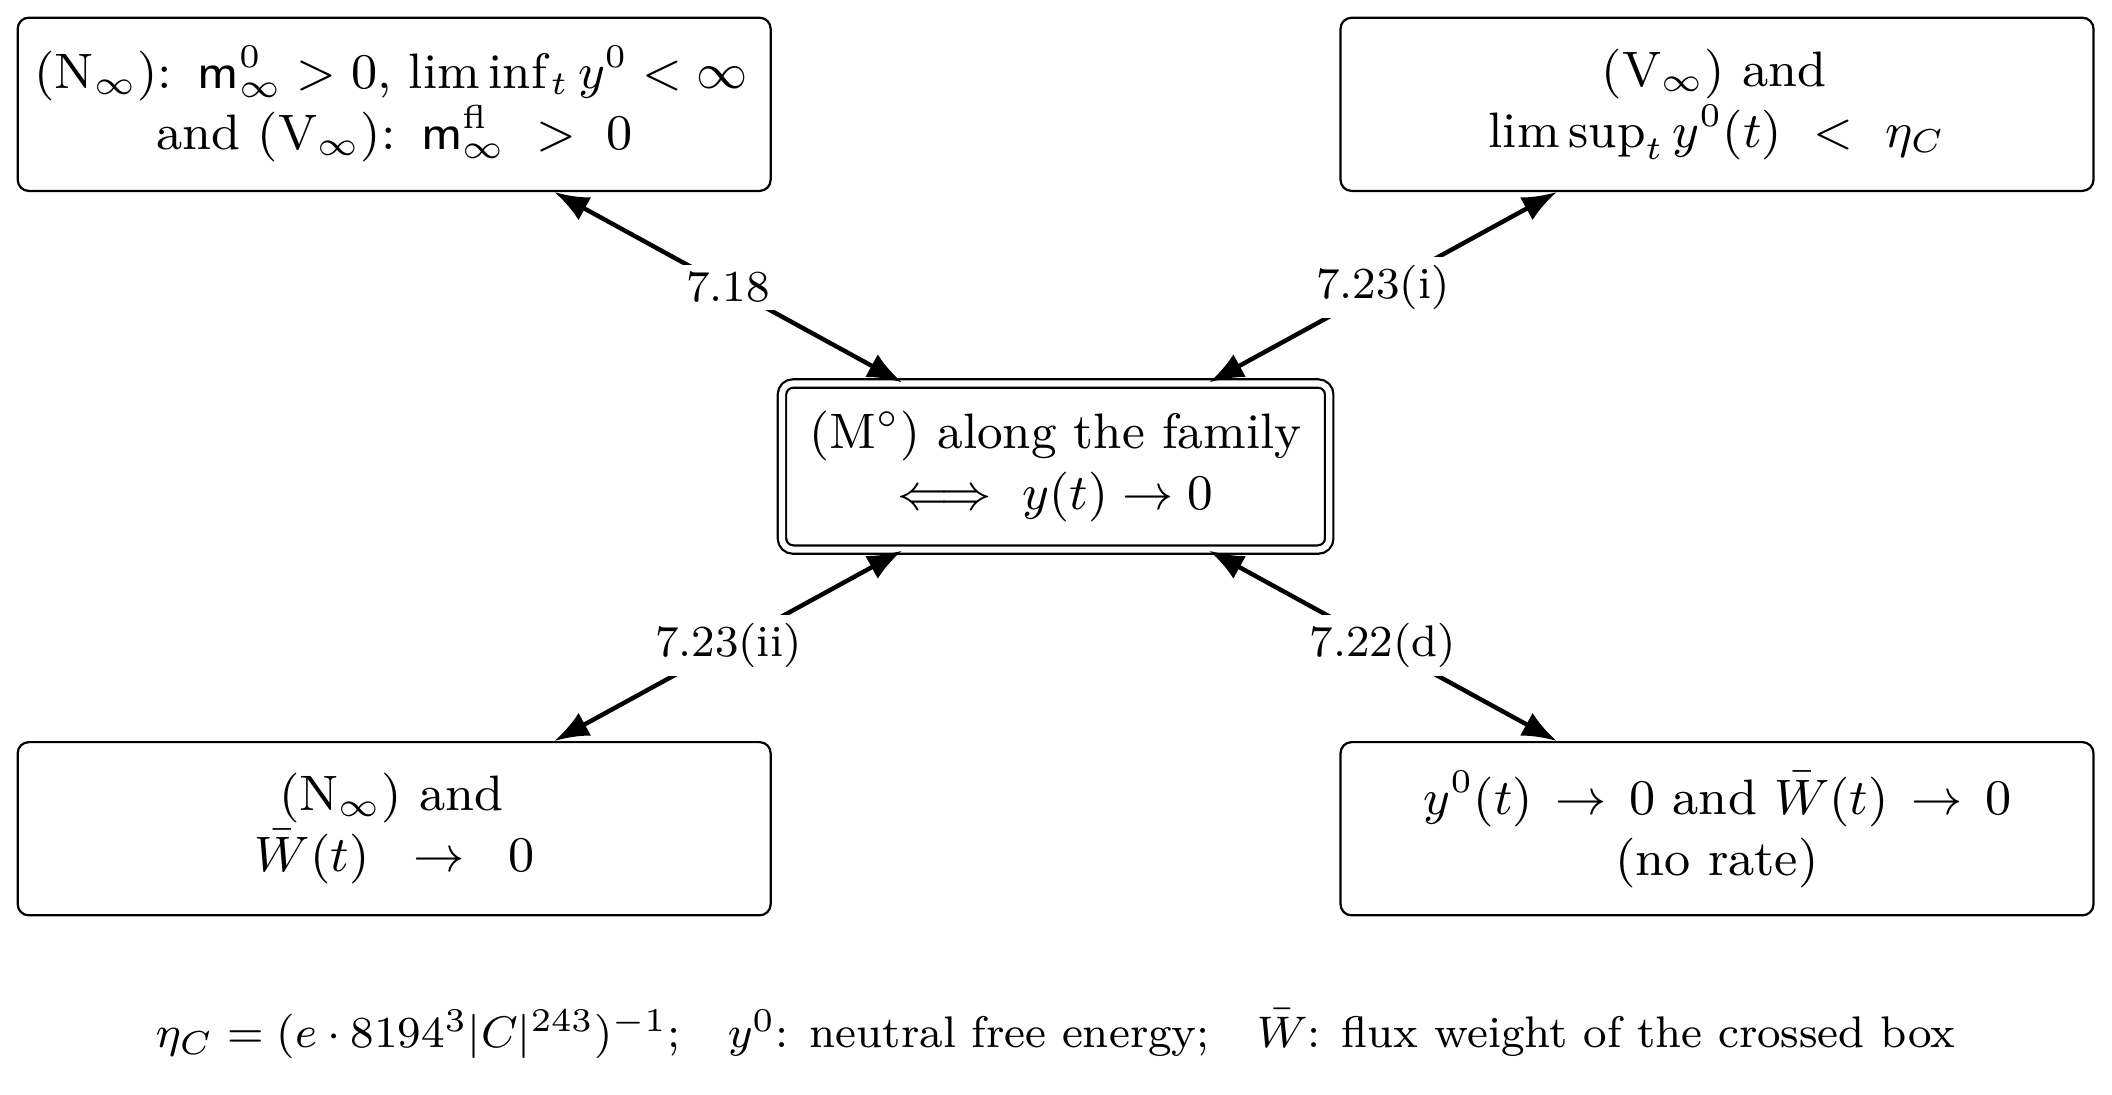
\includegraphics[width=380.0bp]{figures/fig11.png}
\caption{The four equivalent forms of \Mcirc{} along a family. The rate conditions are $\mathsf m^0_\infty>0$ for the centre-neutral sector and $\mathsf m^{\mathrm{fl}}_\infty>0$ for the flux sectors; either may be traded for a thermodynamic quantity tending to $0$, and the lower right form contains no rate. Labels are the results that prove the equivalences; the lower right one also uses \cref{thm:zero-one}\textup{(c)}. None of the five boxes is known for the Wilson theory along the continuum tuning.}
\label{fig:crossed}
\end{figure}

Under the equivalent conditions of \cref{thm:crossed-criteria}, $y^0$, $\bar\varphi$ and $\bar W$ are at most $y\le e^{-\Delta t/2}/64$ for large $t$ (\cref{thm:zero-one}\textup{(c)}), so in (b) the bound $\limsup_ty^0(t)<\eta_C$ may be replaced by $y^0(t)\to0$. Two consequences: in the presence of \textup{(V$_\infty$)}, condition \textup{(N$_\infty$)} is equivalent to $y^0(t)\to0$, a condition that mentions no gap; the factor $1/t_2$ in \cref{lem:sector-thresholds}\textup{(b)} is compensated by the length $\frac12t_1$ over which \eqref{eq:two-number} transports. In the presence of \textup{(N$_\infty$)}, condition \textup{(V$_\infty$)} is equivalent to $\bar W(t)\to0$: the weight of nonzero electric flux in direction $1$ on the crossed box $s_\times(\lfloor Nt\rfloor)$ at time $2\lfloor Nt\rfloor$ tends to $0$ in physical size, which is 't Hooft's criterion for confinement \cite{thooft1979} without a rate. The three families of \cref{prop:criterion-independence} are consistent with this: family (b) has $y^0\equiv0$ but $\bar\varphi\equiv\log8$ and fails \textup{(V$_\infty$)}; family (a) has $\bar W\equiv0$ but $y^0\equiv\log2$ and fails \textup{(N$_\infty$)}; family (c) has $y^0\equiv\infty$. None of the conditions (b)--(d) is known for the Wilson theory along the continuum tuning, and no attempt has been made to optimise $\eta_C$.

\begin{corollary}[a scale-invariant level count]\label{cor:sb-scale-invariant}
Let $n^0_{N,p}(\varepsilon;t)$ be the number of eigenvalues $r$ of $R_{\cube{\lfloor Nt\rfloor}}$ on $\Kspace^0\ominus\C\Omegazero$ in $Z_{N,p}$, with multiplicity, with $N(-\log r)\le\varepsilon$. If there are $K$ and $t_*$ such that $n^0_{N,p}(\varepsilon;t)\le\exp\bigl(K(\varepsilon t)^{3/4}\bigr)$ for all $\varepsilon\ge0$, all $t\ge t_*$ and all large $p$ and $N\ge N_0(p,t)$, then $y^0(t)\le\log\bigl(1+2e^{27K^4/32}\bigr)$ for every $t\ge t_*$. The same holds for the count $n_{N,p}(\varepsilon;t)$ of \cref{rem:sb-count} and $y$ in place of $n^0_{N,p}$ and $y^0$.
\end{corollary}

\begin{proof}
The function $x\mapsto Kx^{3/4}-\frac12x$ on $[0,\infty)$ attains its maximum $\frac{27}{32}K^4$ at $x=(3K/2)^4$, so $n^0_{N,p}(\varepsilon;t)\le Ce^{t\varepsilon/2}$ with $C=e^{27K^4/32}$. With $T=\lfloor Nt\rfloor$, $\theta_N=T/N$ and $\varepsilon_i=N(-\log r_i)$, the computation of \cref{rem:sb-count} applied to $\Zc^0_{\cube T}(T)-1=\sum_ie^{-\theta_N\varepsilon_i}$, the sum over the eigenvalues on $\Kspace^0\ominus\C\Omegazero$, gives $\Zc^0_{\cube T}(T)-1\le C\theta_N/(\theta_N-t/2)$ once $\theta_N>t/2$. As $\theta_N\to t$, $\limsup_N\log\Zc^0_{\cube T}(T)\le\log(1+2C)$. The second statement is \cref{rem:sb-count} with $a=t/2$.
\end{proof}

The count of \cref{cor:sb-scale-invariant} has the form of a Stefan--Boltzmann density of states in a box of side $2t$ with no scale,\footnote{For a gas of massless particles in a box of volume $V$ at temperature $\Theta$ the entropy and the energy scale as $S\propto V\Theta^3$ and $E\propto V\Theta^4$, so $S\propto V^{1/4}E^{3/4}$, and the number of states of energy at most $E$ is $\exp(O(V^{1/4}E^{3/4}))$. With $V\propto t^3$ and $E=\varepsilon$ in physical units this is $\exp(O((\varepsilon t)^{3/4}))$, the count of \cref{cor:sb-scale-invariant}; the exponent $\frac34$ is the one for which the bound on $y^0$ is independent of $t$.} and the bound on $y^0$ it gives does not depend on $t$; the free-gluon reference has the corresponding property $X_\Gharm(T)\le34(N_c^2-1)$ for all $T\ge3$ (\cref{thm:free-gluon}\textup{(b)}). Such a count gives the second half of \textup{(N$_\infty$)} but not $\limsup_ty^0(t)<\eta_C$.

\begin{remark}[bounds proportional to the volume]\label{rem:volume-bounds}
Suppose that $\mathsf m\ge\Delta>0$ and $y(t)\le bt^4$ on $[t_*,\infty)$, and put $\tau=(\Delta/(216b))^{1/3}$. If $\tau\ge t_*$ and $b<\Delta^4/(4096(\log8194)^3)$, then \Mcirc{} holds along the family with $\tzero=\frac32\tau$. Indeed, with $t_1=\tau$ and $t_2=\frac32\tau$ the exponent of \eqref{eq:crossed-exponent} is at most $27b\tau^4-\frac12\Delta\tau=-\frac38\Delta\tau$, since $216b\tau^3=\Delta$, and $\frac38\Delta\tau>\log8194$ is equivalent to $b<\Delta^4/(4096(\log8194)^3)$. A bound of the form $y(t)\le bt^4$ is what a bound per unit of physical four-volume on the cube gives. Through \eqref{eq:crossed-exponent} it yields \Mcirc{} only if its constant is small compared with $\Delta^4$, at the scale $\tau$ of a fixed multiple of the inverse gap: this is a condition in the infrared, and it is not implied by finiteness of $y(t)$ at each $t$. A bound per site of the lattice of mesh $1/N$ gives a constant $b$ that grows at least like $N^4$; the per-site bounds at the unit scale described in \cref{rem:oai-internals} hold on symmetric tori, not on the cubes, and would give errors of order $t^4$ if they held there.
\end{remark}

\subsection{Gaps as decay rates and single-scale reductions}

The conditions of \cref{thm:sector-criterion} pair a gap with a bound on a free energy. This subsection shows that, once the relevant free energy is bounded on a half-line, each gap is exactly the exponential decay rate of the corresponding free energy, and it replaces the thresholds of \cref{thm:crossed-criteria} by thresholds that do not depend on $K$ or $\abs{C}$ and are imposed at a single scale. For $u:(0,\infty)\to[0,\infty]$ put
\[
\lambda[u]=\liminf_{t\to\infty}\,t^{-1}\log\bigl(1/u(t)\bigr)\in[-\infty,\infty],\qquad \log(1/0)=\infty,\quad \log(1/\infty)=-\infty .
\]

\begin{lemma}[sector transport]\label{lem:sector-transport}
\begin{enumerate}[label=\textup{(\alph*)},leftmargin=*]
\item Let $T'\ge T\ge3$ be integers and $s$ a spatial torus with all sides at least $2T$. Then
\begin{equation}\label{eq:sector-transport}
\begin{aligned}
\log\Zc^0_s(T')&\le\Zc^0_s(T')-1\le r_1^0(s)^{T'-T}\bigl(\Zc^0_s(T)-1\bigr),\\
\varphi_s(T')&\le\Zs{s}{T'}-\Zc^0_s(T')\le r^{\mathrm{fl}}(s)^{T'-T}\bigl(\Zs{s}{T}-\Zc^0_s(T)\bigr),
\end{aligned}
\end{equation}
and $\bigl(\Zc^0_s(T)-1\bigr)+\bigl(\Zs{s}{T}-\Zc^0_s(T)\bigr)=\Dexc{s}{T}\le\exp\bigl(\Vol{s}T^{-3}X(T)\bigr)-1$.
\item For a family of systems of this section and $0<t_1<t_2$ with $y(t_1)<\infty$,
\[
y^0(t_2)\le e^{-(t_2-t_1)\mathsf m^0(t_2)}\Bigl(e^{8(t_2/t_1)^3y(t_1)}-1\Bigr),\qquad \bar\varphi(t_2)\le e^{-(t_2-t_1)\mathsf m^{\mathrm{fl}}(t_2)}\Bigl(e^{8(t_2/t_1)^3y(t_1)}-1\Bigr).
\]
\end{enumerate}
\end{lemma}

\begin{proof}
(a) Let $R=R_s$. As in the proof of \cref{lem:sector-thresholds}\textup{(a)}, the restriction of $R$ to $\Kspace^0_s$ has the eigenvalues $1=r^0_0\ge r^0_1\ge r^0_2\ge\cdots\ge0$ with multiplicity, $r^0_0$ belonging to $\Omegazero$, and $\Zc^0_s(M)-1=\sum_{i\ge1}(r^0_i)^M$ for $M\ge1$. Each $r^0_i$ with $i\ge1$ is at most $r^0_1=r_1^0(s)$, so
\[
\Zc^0_s(T')-1=\sum_{i\ge1}(r^0_i)^{T}(r^0_i)^{T'-T}\le r_1^0(s)^{T'-T}\bigl(\Zc^0_s(T)-1\bigr),
\]
and $\log\Zc^0_s(T')\le\Zc^0_s(T')-1$. The operators $P_eR\ge0$, $e\ne0$, act on the mutually orthogonal spaces $\Kspace^e_s$, and by \cref{thm:residue-split}\textup{(a)} $\Zs{s}{M}-\Zc^0_s(M)=\sum_{e\ne0}\Tr\bigl((P_eR)^M\bigr)=\sum_ja_j^M$, where the $a_j$ are the eigenvalues of the $P_eR$, $e\ne0$, with multiplicity. Each $a_j$ is at most $\max_{e\ne0}\norm{P_eR}=r^{\mathrm{fl}}(s)$, which gives the second chain except its first inequality. For that, $\Zc^0_s(T')\ge1$ (\cref{thm:residue-split}\textup{(a)}) gives
\[
\varphi_s(T')=\log\frac{\Zs{s}{T'}}{\Zc^0_s(T')}=\log\Bigl(1+\frac{\Zs{s}{T'}-\Zc^0_s(T')}{\Zc^0_s(T')}\Bigr)\le\Zs{s}{T'}-\Zc^0_s(T').
\]
The identity in the last claim is the definition of $\Dexc{s}{T}=\Zs{s}{T}-1$, and the bound is \eqref{eq:cube-control}.

(b) Fix $p$ with $Y_p(t_1)=\limsup_NX_{N,p}(\lfloor Nt_1\rfloor)<\infty$, and let $T=\lfloor Nt_1\rfloor$, $T'=\lfloor Nt_2\rfloor$, $b_N=(T'-T)/N$ and $c_N=8(T'/T)^3$ as in the proof of \cref{thm:two-number}. The cube $s=\cube{T'}$ has sides $2T'\ge2T$ and $\Vol{s}T^{-3}=c_N$, so (a) gives
\[
\log\Zc^0_{\cube{T'}}(T')\le e^{-b_Na^0_N}\bigl(e^{c_NX_{N,p}(T)}-1\bigr),\qquad \varphi_{\cube{T'}}(T')\le e^{-b_Na^{\mathrm{fl}}_N}\bigl(e^{c_NX_{N,p}(T)}-1\bigr),
\]
with $a^0_N=N(-\log r_1^0(\cube{T'}))$ and $a^{\mathrm{fl}}_N=N(-\log r^{\mathrm{fl}}(\cube{T'}))$. These are the bound of \cref{thm:gapped-transport} used in the proof of \cref{thm:two-number}, with $a^0_N$ and $a^{\mathrm{fl}}_N$ in place of $a_N=N(-\log r_1(\cube{T'}))$, and the passage to the limits $N\to\infty$ and $p\to\infty$ in that proof applies without change.
\end{proof}

\begin{lemma}[neutral bootstrap]\label{lem:neutral-bootstrap}
For a family of systems of this section let $\Delta>0$ and $t_*>0$ satisfy $\mathsf m^0\ge\Delta$ on $[t_*,\infty)$, let $K\ge1$ and $K_1=K+3\log\abs{C}$, and let $t_a\ge t_*$ satisfy $y^0(t_a)\le K$ and $\Delta t_a\ge216K_1$. Then $y^0(t)\le K$ for every $t\ge4t_a$, and $y^0(t)<\exp(27K_1-\Delta t/3)$ for every $t\ge6t_a$.
\end{lemma}

\begin{proof}
Let $G=\{t\ge t_a:y^0(t)\le K\}$. If $t\in G$ and $t_2\in[2t,3t]$, then $y(t)\le y^0(t)+3\log\abs{C}\le K_1$ (\cref{thm:sector-criterion}), $t_2-t\ge t$, $8(t_2/t)^3\le216$ and $t_2\ge t_*$, so \cref{lem:sector-transport}\textup{(b)} gives
\[
y^0(t_2)\le e^{-t\Delta}\bigl(e^{216K_1}-1\bigr)<e^{216K_1-t_a\Delta}\le1\le K .
\]
Hence $[2t,3t]\subset G$ for every $t\in G$. Since $t_a\in G$, induction gives $[2^jt_a,3^jt_a]\subset G$ for $j\ge1$. For $j\ge2$ one has $2^{j+1}\le3^j$, so these intervals overlap, and their union over $j\ge2$ is $[4t_a,\infty)$. For $t\ge6t_a$ put $t_1=\frac23t\ge4t_a$; then $y(t_1)\le K_1$, $t-t_1=\frac13t$ and $8(t/t_1)^3=27$, and \cref{lem:sector-transport}\textup{(b)} gives $y^0(t)\le e^{-\Delta t/3}(e^{27K_1}-1)<e^{27K_1-\Delta t/3}$.
\end{proof}

\begin{theorem}[gaps as decay rates]\label{thm:decay-rates}
\begin{enumerate}[label=\textup{(\alph*)},leftmargin=*]
\item For a family as in \cref{thm:zero-one} with $\liminf_ty(t)<\infty$, $\mathsf m_\infty=\max\{\lambda[y],0\}$.
\end{enumerate}
For a family of systems of this section:
\begin{enumerate}[label=\textup{(\alph*)},leftmargin=*,resume]
\item If $\liminf_ty^0(t)<\infty$, then $\mathsf m^0_\infty=\max\{\lambda[y^0],0\}$, and if $\mathsf m^0_\infty>0$ then $y^0$ is bounded on some interval $[t_*,\infty)$.
\item $\lambda[\bar W]=\lambda[\bar\varphi]\ge0$. If $y^0$ is bounded on some interval $[t_*,\infty)$, then $\mathsf m^{\mathrm{fl}}_\infty=\lambda[\bar\varphi]$.
\item \textup{(N$_\infty$)} holds if and only if $\lambda[y^0]>0$, and then $\mathsf m^0_\infty=\lambda[y^0]$.
\end{enumerate}
\end{theorem}

\begin{proof}
We first show, in each of (a)--(c), that the gap is at most the rate whenever the gap is positive; the converse inequalities follow from the thresholds.

(a) By the opening of \cref{sec:ascent}, $r_1(s)^T\le\Dexc{s}{T}=e^{\XT{s}{T}}\bigl(1-e^{-\XT{s}{T}}\bigr)$, so $T(-\log r_1(s))\ge h(\XT{s}{T})-\XT{s}{T}$, with $h$ as in \cref{lem:sector-thresholds}. This is the first inequality of \cref{lem:sector-thresholds}\textup{(a)} with $\XT{s}{T}$, $r_1$ in place of $\log\Zc^0_s(T)$, $r_1^0$, and the proofs of \cref{lem:sector-thresholds}\textup{(b),(c)} use nothing else; they give $\mathsf m_\infty\ge\lambda[y]$, so $\mathsf m_\infty\ge\max\{\lambda[y],0\}$. Suppose $\mathsf m_\infty>0$. By \cref{cor:gap-sb}, \Mcirc{} holds along the family, and by \cref{thm:zero-one}\textup{(c)} there is $t_*'$ with $y\le1$ on $[t_*',\infty)$. Let $0<\Delta<\mathsf m_\infty$ and $t_*$ with $\mathsf m\ge\Delta$ on $[t_*,\infty)$, and let $k\ge2$ be an integer. For $t\ge\max\{t_*,kt_*'\}$, \eqref{eq:two-number} with $t_1=t/k$ and $t_2=t$ gives $y(t)\le e^{-(1-1/k)\Delta t}(e^{8k^3}-1)$, so $\lambda[y]\ge(1-1/k)\Delta$. Letting $k\to\infty$ and $\Delta\uparrow\mathsf m_\infty$ gives $\lambda[y]\ge\mathsf m_\infty$. Hence $\mathsf m_\infty=\max\{\lambda[y],0\}$ in both cases.

(b) \Cref{lem:sector-thresholds}\textup{(c)} gives $\mathsf m^0_\infty\ge\max\{\lambda[y^0],0\}$. Suppose $\mathsf m^0_\infty>0$, and let $0<\Delta<\mathsf m^0_\infty$ and $t_*$ with $\mathsf m^0\ge\Delta$ on $[t_*,\infty)$. Choose $K\ge1$ with $y^0(t)\le K$ for arbitrarily large $t$, and $t_a\ge\max\{t_*,216K_1/\Delta\}$ with $y^0(t_a)\le K$, where $K_1=K+3\log\abs{C}$. By \cref{lem:neutral-bootstrap}, $y^0\le K$ on $[4t_a,\infty)$; in particular $y^0$ is bounded on a half-line, and $y\le K_1$ there by \cref{thm:sector-criterion}. For an integer $k\ge2$ and $t\ge\max\{t_*,4kt_a\}$, \cref{lem:sector-transport}\textup{(b)} with $t_1=t/k$ and $t_2=t$ gives $y^0(t)\le e^{-(1-1/k)\Delta t}(e^{8k^3K_1}-1)$, so $\lambda[y^0]\ge(1-1/k)\Delta$, and as in (a) $\lambda[y^0]\ge\mathsf m^0_\infty$.

(c) By \cref{lem:sector-thresholds}\textup{(d)}, $\bar W\le-\log(1-\bar W)\le\bar\varphi$, so $\lambda[\bar W]\ge\lambda[\bar\varphi]$; and $\bar\varphi\le3\log\abs{C}$ by \cref{thm:residue-split}\textup{(a)}, so $\lambda[\bar\varphi]\ge0$. If $\lambda[\bar W]>0$, then $\bar W(t)\to0$, and for large $t$, $3\bar W(t)\le\frac12$ and $\bar\varphi(t)\le-\log(1-3\bar W(t))\le6\bar W(t)$, because $-\log(1-x)\le2x$ on $[0,\frac12]$ by convexity; hence $\lambda[\bar\varphi]\ge\lambda[\bar W]$. If $\lambda[\bar W]=0$, then $0\le\lambda[\bar\varphi]\le\lambda[\bar W]=0$. This proves the first claim. Let now $y^0\le K$ on $[t_*,\infty)$; then $y\le K_1=K+3\log\abs{C}$ there by \cref{thm:sector-criterion}, and \cref{lem:sector-thresholds}\textup{(c)} gives $\mathsf m^{\mathrm{fl}}_\infty\ge\lambda[\bar\varphi]$. If $\mathsf m^{\mathrm{fl}}_\infty>0$, let $0<\Delta<\mathsf m^{\mathrm{fl}}_\infty$ and $t_{**}\ge t_*$ with $\mathsf m^{\mathrm{fl}}\ge\Delta$ on $[t_{**},\infty)$; for an integer $k\ge2$ and $t\ge kt_{**}$, \cref{lem:sector-transport}\textup{(b)} with $t_1=t/k$ gives $\bar\varphi(t)\le e^{-(1-1/k)\Delta t}(e^{8k^3K_1}-1)$, and as in (a) $\lambda[\bar\varphi]\ge\mathsf m^{\mathrm{fl}}_\infty$. If $\mathsf m^{\mathrm{fl}}_\infty=0$, then $0\le\lambda[\bar\varphi]\le\mathsf m^{\mathrm{fl}}_\infty=0$.

(d) If \textup{(N$_\infty$)} holds, (b) gives $\lambda[y^0]=\mathsf m^0_\infty>0$. If $\lambda[y^0]>0$, then $y^0(t)\to0$, so $\liminf_ty^0(t)<\infty$, and (b) gives $\mathsf m^0_\infty=\lambda[y^0]>0$.
\end{proof}

Part (d) shows that the two halves of \textup{(N$_\infty$)} are one statement: the neutral free energy of the cube of physical side $2t$ decays exponentially in $t$, and its rate is the neutral gap. Without the bound on $y^0$ the identities fail: for the rings of \cref{prop:criterion-independence}\textup{(c)}, $\mathsf m^0\equiv\Delta$ while $y^0\equiv\infty$ and $\lambda[y^0]=-\infty$. By (a), \cref{thm:zero-one}\textup{(c)} and \cref{cor:gap-sb}, along a family with $\liminf_ty(t)<\infty$ the free energy $y$ decays at the exact rate $\mathsf m_\infty$ under \Mcirc{}, and $\lambda[y]\le0$ otherwise.

\begin{corollary}[sharp crossed criteria]\label{cor:sharp-crossed}
For a family of systems of this section let $c_*=\frac13\bigl(1-e^{-x_c}\bigr)$; then $c_*>8\cdot10^{-5}$.
\begin{enumerate}[label=\textup{(\roman*)},leftmargin=*]
\item \Mcirc{} holds along the family if and only if \textup{(V$_\infty$)} holds and $\limsup_{t\to\infty}y^0(t)<x_c$. If \textup{(V$_\infty$)} holds and $y^0$ is bounded on some interval $[t_*,\infty)$, then \Mcirc{} holds along the family if and only if $\liminf_{t\to\infty}y^0(t)<x_c$.
\item \Mcirc{} holds along the family if and only if \textup{(N$_\infty$)} holds and $\liminf_{t\to\infty}\bar W(t)<c_*$, and if and only if \textup{(N$_\infty$)} holds and $\liminf_{t\to\infty}\bar\varphi(t)<x_c$. Under \Mcirc{}, $\lambda[\bar W]=\lambda[\bar\varphi]=\mathsf m^{\mathrm{fl}}_\infty>0$.
\item Let $t_1>0$, $\Delta>0$, $K\ge0$ and $K_1=K+3\log\abs{C}$ satisfy $y^0(\frac23t_1)\le K$ and $\Delta t_1\ge3(27K_1+\log16388)$. If $\mathsf m^{\mathrm{fl}}(t_1)\ge\Delta$ and $y^0(t_1)<1/16388$, or if $\mathsf m^0(t_1)\ge\Delta$ and $\bar W(t_1)<1/49167$, then \Mcirc{} holds along the family with $\tzero=t_1$.
\end{enumerate}
\end{corollary}

\begin{proof}
Since $1-e^{-x}\ge x-\frac12x^2$ for $x\ge0$ and $x_c>1/4160$ (\cref{thm:zero-one}), $3c_*\ge\frac1{4160}-\frac1{2\cdot4160^2}=\frac{8319}{34611200}$, and $8319\cdot12500=103987500>3\cdot34611200$, so $c_*>1/12500$.

(i) If \Mcirc{} holds, \cref{thm:sector-criterion} gives \textup{(V$_\infty$)} and \cref{thm:zero-one}\textup{(c)} gives $y^0\le y\to0$. If $\limsup_ty^0(t)<x_c$, then $y^0$ is bounded on a half-line and $\liminf_ty^0(t)<x_c$, so the first claim follows from the second. For the second, \cref{thm:decay-rates}\textup{(c)} gives $\lambda[\bar\varphi]=\mathsf m^{\mathrm{fl}}_\infty>0$, so $\bar\varphi(t)\to0$. By \cref{lem:sector-thresholds}\textup{(d)}, $y\le y^0+\bar\varphi$, so $\liminf_ty(t)\le\liminf_ty^0(t)+\lim_t\bar\varphi(t)=\liminf_ty^0(t)$. If this is less than $x_c$, then $y(t)<x_c$ for some $t$, and \cref{thm:zero-one}\textup{(c)} gives \Mcirc{}. Conversely \Mcirc{} gives $y^0\to0$.

(ii) If \Mcirc{} holds, \cref{thm:sector-criterion} gives \textup{(N$_\infty$)} and \cref{lem:sector-thresholds}\textup{(d)} and \cref{thm:zero-one}\textup{(c)} give $\bar W\le\bar\varphi\le y\to0$. Suppose \textup{(N$_\infty$)}. By \cref{thm:decay-rates}\textup{(d)}, $\lambda[y^0]>0$, so $y^0(t)\to0$, and $\liminf_ty(t)\le\lim_ty^0(t)+\liminf_t\bar\varphi(t)=\liminf_t\bar\varphi(t)$. If $\liminf_t\bar\varphi(t)<x_c$, then $y(t)<x_c$ for some $t$ and \Mcirc{} holds by \cref{thm:zero-one}\textup{(c)}. If $\bar W(t_n)\le c'<c_*$ along a sequence $t_n\to\infty$, then by \cref{lem:sector-thresholds}\textup{(d)} $\bar\varphi(t_n)\le-\log(1-3c')<-\log(1-3c_*)=x_c$, so $\liminf_t\bar\varphi(t)<x_c$. Under \Mcirc{}, $y^0\to0$ is bounded on a half-line and $\mathsf m^{\mathrm{fl}}_\infty>0$ by \cref{thm:sector-criterion}, and \cref{thm:decay-rates}\textup{(c)} gives the rates.

(iii) Put $t'=\frac23t_1$. By \cref{thm:sector-criterion}, $y(t')\le y^0(t')+3\log\abs{C}\le K_1$, and $t_1-t'=\frac13t_1$ and $8(t_1/t')^3=27$. In the first case \cref{lem:sector-transport}\textup{(b)} gives
\[
\bar\varphi(t_1)\le e^{-\Delta t_1/3}\bigl(e^{27K_1}-1\bigr)<e^{27K_1-\Delta t_1/3}\le\tfrac1{16388}.
\]
In the second case it gives $y^0(t_1)<1/16388$ in the same way, and since $3/49167=1/16389$, \cref{lem:sector-thresholds}\textup{(d)} gives $\bar\varphi(t_1)\le-\log(1-3\bar W(t_1))<-\log\bigl(1-\frac1{16389}\bigr)=\log\bigl(1+\frac1{16388}\bigr)\le\frac1{16388}$. In both cases $y(t_1)\le y^0(t_1)+\bar\varphi(t_1)<\frac2{16388}=\frac1{8194}$ by \cref{lem:sector-thresholds}\textup{(d)}. As in the proof of \cref{thm:two-number}, $y(t_1)<1/8194$ gives \Mcirc{} along the family with $\tzero=t_1$.
\end{proof}

In (i) and (ii) the constant $\eta_C$ of \cref{thm:crossed-criteria} is replaced by the critical value $x_c$ of \cref{thm:zero-one}, which depends neither on $\abs{C}$ nor on any rate, and the limit superior by a limit inferior. The criteria have the form of dichotomies. Under \textup{(N$_\infty$)}, either 't Hooft's flux weight on the crossed box satisfies $\liminf_t\bar W(t)\ge c_*$, or it tends to $0$ exponentially, at the rate $\mathsf m^{\mathrm{fl}}_\infty$, and \Mcirc{} holds; no intermediate behaviour of $\bar W$ is possible. Under \textup{(V$_\infty$)}, with $y^0$ bounded on a half-line, either $y^0(t)\ge x_c-\bar\varphi(t)$ for all $t>0$, with $\bar\varphi(t)\to0$, or $y^0$ tends to $0$ exponentially. Part (iii) needs one value of a gap, one bound on $y^0$ at the scale $\frac23t_1$, and one small number at the scale $t_1$. In its second case the small number is the flux weight $\bar W(t_1)$, a ratio of twisted to untwisted partition functions on one cube, and the threshold $1/49167$ does not depend on $K$, unlike the threshold $(3\cdot8194^3e^{108K_1})^{-1}$ of \cref{thm:crossed-criteria}\textup{(ii)}. None of the hypotheses of \cref{cor:sharp-crossed} is known for the Wilson theory along the continuum tuning.

The flux weight need not decrease with the size of the cube, so the smallness of $\bar W(t_1)$ in (iii) cannot be read off from its value at a smaller scale.

\begin{proposition}[the flux weight is not monotone]\label{prop:flux-nonmonotone}
Let $G=C=\{\pm1\}\subset\U(1)$ and $f(g)=e^{10g}$. Then $W^{\mathrm P}_*(3)<W^{\mathrm P}_*(6)$. Hence no inequality $W^{\mathrm P}_*(T')\le W^{\mathrm P}_*(T)$ for integers $T'\ge T\ge3$ holds for all systems of this section.
\end{proposition}

\begin{proof}
Let $s=\cube T$ and $\rho_T=Z_s(T;(-1)_{(1)})/\Zpart{s}{T}$. By \cref{thm:residue-split}\textup{(f)}, \eqref{eq:cg-Wj} and \cref{lem:centre-operators}\textup{(c)}, as in the proof of \cref{thm:residue-split}\textup{(d)}, $1-W^{\mathrm P}_*(T)=1-W_1(s,T)=\frac12(1+\rho_T)$, so $W^{\mathrm P}_*(T)=\frac12(1-\rho_T)$, and it suffices to show $\rho_6<\rho_3$. In the notation of the proof of \cref{lem:z2-violation}, with $\beta'=10$ and the torus $\cube T\times T$, $\rho_T=\Phi(c_T)/\Phi(0)$, where $c_T\ne0$ is the class of the stack $S_{14}$, and by \cref{lem:centre-operators}\textup{(b)} the twisted integral does not depend on the stack.

\emph{Upper bound at $T=6$.} Step~2 of that proof gives $\rho_6\le48\cdot6^4e^{-20}q^{71}/(1-q)$ with $q=400e^{-20}$; with $\log q=\log400-20<-14.0085$ this gives $\log\rho_6<-1003.5$.

\emph{Lower bound at $T=3$.} The torus $\cube3\times3$ has sides $(6,6,6,3)$ and $6\cdot648=3888$ plaquettes. For $0\le a\le5$ and $0\le b\le2$ let $S(a,b)$ be the set of the $36$ plaquettes of the $(1,4)$-plane with $x_1=a$ and $x_4=b$. If $\sigma$ is the indicator of the $1$-links $(x,1)$ with $x_1=a$, $x_4=b+1$, then a $(1,\nu)$-plaquette with $\nu\in\{2,3\}$ contains two or none of these links, and a $(1,4)$-plaquette with base point $y$ contains exactly one of them if and only if $y_1=a$ and $y_4\in\{b,b+1\}$; so $d\sigma=S(a,b)+S(a,b+1)$. Likewise the indicator of the $4$-links $(x,4)$ with $x_1=a+1$, $x_4=b$ has coboundary $S(a,b)+S(a+1,b)$. Hence the $18$ distinct sets $S(a,b)$ are cocycles in the class $c_3$ of $S_{14}=S(5,2)$, and $\Phi(c_3)\ge18e^{-20\cdot36}=18e^{-720}$. For the upper bound on $\Phi(0)$, every cocycle $e$ is the disjoint union of its adjacency components, which are distinct nonempty connected cocycles (Step~2 of the proof of \cref{lem:z2-violation}), and $e$ determines them. So
\[
\Phi(0)\le\sum_ee^{-20\abs e}\le\prod_{D}\bigl(1+e^{-20\abs{D}}\bigr)\le\exp\Bigl(\sum_{D}e^{-20\abs{D}}\Bigr),
\]
the sum over all cocycles $e$ and the products and sums over nonempty connected cocycles $D$. With at most $3888\cdot20^{2(n-1)}$ connected sets of $n$ plaquettes, $\sum_{D}e^{-20\abs{D}}\le3888e^{-20}/(1-q)<10^{-5}$. Hence $\log\rho_3\ge\log18-720-10^{-5}>-717.12$.

So $\log\rho_6<-1003.5<-717.12<\log\rho_3$, and $W^{\mathrm P}_*(3)<W^{\mathrm P}_*(6)$.
\end{proof}

The difference is of order $e^{-717}$, and both values lie within $2.3\cdot10^{-15}$ of $\frac12=1-1/\abs{C}$ by \cref{lem:z2-violation}. In this system $\rho_T$ is at most the bound of Step~2 of that proof, which tends to $0$ as $T\to\infty$, so the flux weight tends to its ceiling $\frac12$ as the cube grows. A monotonicity of $T\mapsto W^{\mathrm P}_*(T)$ along the continuum tuning would therefore have to use a property that this system lacks, as in \cref{prop:no-vortex-comparison}.

\begin{remark}[the flux weight and the tokens]\label{rem:token-flux}
Let $G_0\subset\U(m_0)$ be closed with simple Lie algebra and $-\mathbf 1_{m_0}\in G_0$, let $k\ge1$, and let $G'=\{\operatorname{diag}(g,h\mathbf 1_k)\}\subset\U(m_0+k)$ be the group of the paragraph on connectedness in \cref{sec:constructed}, with the Wilson weight at coupling $\betaW$ and $C'=\{\pm\mathbf 1_{m_0+k}\}$. If $\beta'=\betaW k/(m_0+k)\ge4$, then $W'^{\mathrm P}_*(T)\ge\frac12(1-\Gamma)>\frac12-1.2\cdot10^{-15}$ for every $T\ge3$, with $\Gamma$ of \cref{lem:z2-violation}. Indeed $-\mathbf 1_{m_0+k}=\operatorname{diag}(-\mathbf 1_{m_0},-\mathbf 1_k)$, and the factorisation of the Wilson measure in that paragraph applies to the integrand of \eqref{eq:cg-twisted}, so the twist ratio of $G'$ on $\cube T\times T$ is the product $\rho_{G_0}\rho_{\Z/2}$ of the twist ratios of the $G_0$ system at coupling $\betaW m_0/(m_0+k)$ with $C_0=\{\pm\mathbf 1_{m_0}\}$ and of the $\Z/2$ system at $\beta'$. By \cref{lem:centre-operators}\textup{(c)}, $0<\rho_{G_0}\le1$, and Steps~2 and~3 of the proof of \cref{lem:z2-violation} give $\rho_{\Z/2}\le\Gamma$, as in the proof of \cref{prop:no-vortex-comparison}; and $W'^{\mathrm P}_*=\frac12(1-\rho_{G_0}\rho_{\Z/2})$ as in the proof of \cref{prop:flux-nonmonotone}. So along every tuning of $G'$ with $\betaW\to\infty$, $\bar W'(t)\ge\frac12(1-\Gamma)$ for every $t>0$, while insertions supported on the $G_0$ block have the same moments as for $G_0$. Condition $\bar W(t)\to0$ of \cref{thm:crossed-criteria}\textup{(d)} is therefore not determined by the correlators of the tokens: for $G_0=\SU(2)$, whose centre element $-\mathbf 1_2$ acts on the first block as $-\mathbf 1_{m_0+k}$ does, a proof of it must use connectedness of the gauge group.
\end{remark}
\section{Proved ranges of the datum: strong coupling, large $N_c$, two dimensions}\label{sec:ranges}

This section proves the datum at strong coupling for every compact group, for $\SU(N_c)$ at $\beta=\betaW/N_c^2<1/48$, a coupling range uniform in $N_c$ (with $T_*=O(\log N_c)$), and for two-dimensional $\SU(2)$ at every coupling. These are strong-coupling statements and do not touch the continuum tuning. The first two proofs compare the tori of time extents $T$ and $2T$ by a Dobrushin-type contraction and integrate the response in the coupling; the third is exact. \Cref{fig:datum-map} places the ranges in the $(\betaW,\Tzero)$-plane together with the lower bound on the base scale of \cref{sec:necessary}.

\paragraph{Setting}
$G\subset\U(d)$ is a compact group with normalised Haar measure, $s=(s_1,s_2,s_3)$ a spatial torus with all sides at least $3$, $V=\Vol{s}$, and for an integer $t\ge3$, $\Lambda_t=(\Z/s_1)\times(\Z/s_2)\times(\Z/s_3)\times(\Z/t)$ has links $E_t$ and plaquettes $P_t$, $\abs{P_t}=6Vt$. The Wilson measure $\mu_{s,t}=\mu_{s,t;\betaW}$ on $G^{E_t}$ has density
\begin{equation}\label{eq:ranges-weight}
\Zpart{s}{t}^{-1}\exp\Bigl(\frac{\betaW}{d}\sum_{p\in P_t}\ReTr U_p\Bigr)
\end{equation}
with respect to Haar measure; for $G=\SU(N_c)$ this is \eqref{eq:wilson-weight} with $\beta=\betaW/N_c^2$. Then $\psiT{s}{T}=2\log\Zpart{s}{T}-\log\Zpart{s}{2T}\ge0$ by \cref{lem:transfer-matrix,lem:E1-E3}; a factor $c^{Vt}$ in $\Zpart{s}{t}$ cancels in $\psi$.

Two distinct links are \emph{partners} if they lie in a common plaquette. As all sides of $\Lambda_t$ are at least $3$, every link lies in six plaquettes, has $18$ partners and shares exactly one plaquette with each. A spatial link at time $\tau$ has \emph{time coordinate} $\tau$, a temporal link from $\tau$ to $\tau+1$ has time coordinate $\tau+\frac12$ (on $\R/t\Z$). A spatial link has $12$, $4$, $2$ partners at time distance $0$, $\frac12$, $1$; a temporal link has $6$ and $12$ at distance $0$ and $\frac12$. A temporal plaquette has \emph{base} $\tau$ if its sites lie at times $\tau,\tau+1$. The \emph{orientation} of a plaquette is its coordinate plane. Translations preserve $\mu_{s,t}$ and act transitively on the plaquettes of each orientation $o$, so $w_t(o;u)=\mu_{s,t;u}(d^{-1}\ReTr U_p)$, $p$ of orientation $o$, is well defined. Since $\partial_u\log\Zpart{s}{t}=Vt\sum_ow_t(o;u)$ and $\psi=0$ at $u=0$,
\begin{equation}\label{eq:ranges-response}
\psiT{s}{T}\big|_{\betaW}=2VT\int_0^{\betaW}\sum_{o}\bigl(w_T(o;u)-w_{2T}(o;u)\bigr)\dd u ,
\end{equation}
the response formula of \cref{ms:prop:response}. The ranges below are proved for the \emph{window inequality}
\begin{equation}\label{eq:ranges-window}
\psiT{s}{T}\le\frac{\Vol{s}}{161\,(48T)^3}.
\end{equation}
On $\Wwin_{T}$ it is \eqref{ms:eq:rational-condition} at $\Tzero=T$. At $s=\cube{T}$ it reads $\psiT{\cube{T}}{T}\le1/2225664<\dconstinl$, so it implies \eqref{eq:datum-M} at $\Tzero=T$, hence \eqref{eq:datum-B} by \cref{lem:purity-conversion}, and \cref{thm:ascent} applies.

\subsection{A weighted Dobrushin comparison}

Let $S$ be finite and, for $x\in S$, let $X_x$ be a compact metric space with a Borel probability measure $\lambda_x$ and a bounded Borel metric $\varrho_x$ (which need not induce the topology; the discrete metric is allowed). On $\Omega=\prod_xX_x$, $\lambda=\bigotimes_x\lambda_x$, let $\omega^{x\to\xi}$ be $\omega$ with $x$-coordinate replaced by $\xi$. A probability measure $\mu$ with continuous density $e^H/\int e^H\dd\lambda$ has the single-site conditional laws
\begin{equation}\label{eq:dob-conditional}
\gamma^\mu_x(\dd\xi\,|\,\omega)=e^{H(\omega^{x\to\xi})}\lambda_x(\dd\xi)\Big/\textstyle\int e^{H(\omega^{x\to\xi'})}\lambda_x(\dd\xi').
\end{equation}
For probability measures $\gamma,\gamma'$ on $X_x$ let $W_x(\gamma,\gamma')$ be the supremum of $\abs{\gamma(g)-\gamma'(g)}$ over bounded Borel $g$ with $\abs{g(\xi)-g(\xi')}\le\varrho_x(\xi,\xi')$; it is at most the Kantorovich distance and equals $\TV$ for the discrete metric. For bounded Borel $f$ on $\Omega$ let $\delta_x(f)=\sup\abs{f(\omega)-f(\omega')}/\varrho_x(\omega_x,\omega'_x)$ over pairs $\omega\neq\omega'$ that differ only at $x$.

\begin{lemma}[weighted Dobrushin comparison]\label{lem:dobrushin}
Let $\mu,\nu$ be probability measures on $\Omega$ with strictly positive continuous densities with respect to $\lambda$. Put
\[
C_{xy}=\sup\frac{W_x\bigl(\gamma^\mu_x(\cdot|\omega),\gamma^\mu_x(\cdot|\omega')\bigr)}{\varrho_y(\omega_y,\omega'_y)}\ (y\neq x),\qquad C_{xx}=0,\qquad
b_x=\sup_\omega W_x\bigl(\gamma^\mu_x(\cdot|\omega),\gamma^\nu_x(\cdot|\omega)\bigr),
\]
the first supremum over pairs that differ only at $y$, and suppose that $\rho:S\to(0,\infty)$ and $\theta\in[0,1)$ satisfy
\begin{equation}\label{eq:dob-hyp}
\textstyle\sum_{y}C_{xy}\,\rho_y\le\theta\rho_x\quad\text{and}\quad b_x\le\rho_x\qquad(x\in S).
\end{equation}
Let $x_1,x_2,\dots$ run through $S$ cyclically, $\tau_xf(\omega)=\int f(\omega^{x\to\xi})\,\gamma^\mu_x(\dd\xi|\omega)$, $f_0=f$, $f_k=\tau_{x_k}f_{k-1}$. If $f$ is bounded Borel and every $\delta_x(f)$ is finite, then $f_k\to\mu(f)$ uniformly and
\begin{equation}\label{eq:dob-conclusion}
\abs{\nu(f)-\mu(f)}\le\sum_{k\ge1}b_{x_k}\,\delta_{x_k}(f_{k-1})\le\frac{1}{1-\theta}\sum_{x\in S}\rho_x\,\delta_x(f).
\end{equation}
\end{lemma}

This is the weighted form of Dobrushin's comparison theorem \cite{dobrushin1970,follmer1982,kunsch1982}; we include the proof.

\begin{proof}
Let $\tau^\nu_x$ be $\tau_x$ with $\gamma^\nu_x$ in place of $\gamma^\mu_x$; both map bounded Borel functions to bounded Borel functions. (1) $\mu(\tau_xg)=\mu(g)$ and $\nu(\tau^\nu_xg)=\nu(g)$, by Fubini's theorem and \eqref{eq:dob-conditional}. (2) $\abs{\nu(g)-\nu(\tau_xg)}=\abs{\nu(\tau^\nu_xg-\tau_xg)}\le b_x\delta_x(g)$, since $\xi\mapsto g(\omega^{x\to\xi})$ has Lipschitz constant $\delta_x(g)$ for $\varrho_x$. (3) $\delta_x(\tau_xg)=0$ and, for $y\neq x$, $\delta_y(\tau_xg)\le\delta_y(g)+C_{xy}\delta_x(g)$: for $\omega,\omega'$ that differ only at $y$,
\[
\tau_xg(\omega)-\tau_xg(\omega')=\int\bigl[g(\omega^{x\to\xi})-g(\omega'^{x\to\xi})\bigr]\gamma^\mu_x(\dd\xi|\omega)+\int g(\omega'^{x\to\xi})\bigl[\gamma^\mu_x(\dd\xi|\omega)-\gamma^\mu_x(\dd\xi|\omega')\bigr],
\]
and the two terms are at most $\delta_y(g)\varrho_y(\omega_y,\omega'_y)$ and $\delta_x(g)C_{xy}\varrho_y(\omega_y,\omega'_y)$.

Put $\varepsilon_k=\delta_{x_k}(f_{k-1})$ and $\Phi_k=\sum_y\rho_y\delta_y(f_k)$; $\Phi_0<\infty$ because $S$ is finite and every $\delta_y(f)$ is finite, and $\Phi_k<\infty$ follows inductively from the next inequality. By (3) and \eqref{eq:dob-hyp}, $\Phi_k\le\Phi_{k-1}-\rho_{x_k}\varepsilon_k+\varepsilon_k\sum_yC_{x_ky}\rho_y\le\Phi_{k-1}-(1-\theta)\rho_{x_k}\varepsilon_k$, so
\begin{equation}\label{eq:dob-sum}
\textstyle\sum_{k\ge1}\rho_{x_k}\varepsilon_k\le\Phi_0/(1-\theta)<\infty
\end{equation}
and $\varepsilon_k\to0$, since $\min\rho>0$. Each $C_{xy}\le\theta\rho_x/\rho_y$ is finite; let $\bar C=\max C_{xy}$ and $m=\abs S$. In the $n$-th sweep, $\delta_y=0$ right after $y$ is updated, and at each later step $k$ of the sweep $\delta_y$ grows by at most $C_{x_ky}\varepsilon_k$; so $\delta_y(f_{nm})\le\bar C\sum_{k=(n-1)m+1}^{nm}\varepsilon_k\to0$ for every $y$. Hence $\osc(f_{nm})\le\sum_y\delta_y(f_{nm})\sup\varrho_y\to0$. As $\tau_xg$ averages values of $g$, $\osc(f_k)$ is nonincreasing, so $\osc(f_k)\to0$, and since $\mu(f_k)=\mu(f)$ by (1), $\sup\abs{f_k-\mu(f)}\le\osc(f_k)\to0$. Finally (2) gives $\abs{\nu(f)-\nu(f_K)}\le\sum_{k\le K}b_{x_k}\varepsilon_k$, and $\nu(f_K)\to\mu(f)$; this is the first inequality of \eqref{eq:dob-conclusion}, and the second follows from $b\le\rho$ and \eqref{eq:dob-sum}.
\end{proof}

\subsection{Strong coupling for every compact group}

\begin{theorem}[strong coupling]\label{thm:strong-coupling}
Let $G\subset\U(d)$ be a compact group, let every side of $s$ be at least $3$, $T\ge3$ and $\betaW\ge0$. Put $c(\betaW)=\tanh\betaW$ for general $G$ and $c(\betaW)=\betaW/4$ for $G=\SU(2)$. For $z\ge1$ let $\kappa(z)=\max\{12+4z+2z^2,\ 6+12z\}$, and suppose that $\theta:=c(\betaW)\kappa(z)<1$. Then
\begin{equation}\label{eq:sc-bound}
0\le\psiT{s}{T}\le\frac{96\,\betaW\,T\,\Vol{s}}{1-\theta}\,z^{\,1-2\lfloor T/2\rfloor}.
\end{equation}
\end{theorem}

\begin{proof}
Fix $u\in[0,\betaW]$ and an orientation $o$, and write $c=c(u)$; as $c$ is nondecreasing, $c\,\kappa(z)\le\theta$.

\emph{Step 1: two measures.} Let $\mu=\mu_{s,2T;u}$, and let $\nu$ be the law of two independent copies of $\mu_{s,T;u}$ placed on $G^{E_{2T}}$: copy~1 on the links with time coordinate in $[0,T)$, copy~2 on those in $[T,2T)$, a link with time coordinate $\tau$ carrying the link of $\Lambda_T$ in the same position with time coordinate $\tau\bmod T$. Then $\nu$ has a density of the form \eqref{eq:ranges-weight} for the plaquette set obtained from $P_{2T}$ by rewiring the temporal plaquettes of bases $T-1$ and $2T-1$, whose far spatial link is taken at time $0$ instead of $T$, respectively at time $T$ instead of $0$. Let $B_t$ be the temporal links with time coordinate $T-\frac12$ or $2T-\frac12$, and $B_s$ the spatial links at times $T-1,T,2T-1,0$. Outside $B_t\cup B_s$ the conditional laws under $\mu$ and $\nu$ agree; a link of $B_s$ has exactly one of its six plaquette terms replaced by another one, a link of $B_t$ all six. Let $t_0=\lfloor(T-2)/2\rfloor$ and let $p$ be a plaquette of orientation $o$ whose links have time coordinates in $[t_0,t_0+1]$. As $t_0\le T-2$, $p$ lies in copy~1 and is not rewired, so $f=d^{-1}\ReTr U_p$ has $\nu(f)=w_T(o;u)$ and $\mu(f)=w_{2T}(o;u)$.

\emph{Step 2: coefficients, general $G$.} Use the discrete metric, so $W=\TV$, and put $D=1$. If two probability densities are proportional to $e^{\varphi}$ and $e^{\varphi+g}$, their ratio $\ell$ has mean one under the first and values in $[m,M]$ with $m\le1\le M$, $M/m\le K:=e^{\osc g}$; as $t\mapsto(t-1)_+$ lies below its chord on $[m,M]$ and the chord bound increases in $M$,
\[
\TV=\int(\ell-1)_+\le\frac{(M-1)(1-m)}{M-m}\le\max_{0<m'\le1}\frac{(Km'-1)(1-m')}{(K-1)m'}=\frac{\sqrt K-1}{\sqrt K+1},
\]
which is $\tanh(\osc g/4)$; this is the chord argument of \cref{ms:lem:tv}. Changing a partner $y$ of $x$ changes one of the six plaquette terms of the conditional density of $U_x$, by a function with values in $[-2u,2u]$; so $C_{xy}\le\tanh u=c$, and $C_{xy}=0$ for non-partners. Likewise $b_y\le c$ on $B_s$, $b_y\le1$ on $B_t$, $b_y=0$ elsewhere, and $\delta_x(f)\le2$ on the links of $p$.

\emph{Step 3: coefficients, $\SU(2)$.} Identify $\SU(2)$ with the unit sphere $S^3\subset\mathbb H\cong\R^4$, so $\frac12\ReTr(UV)=\ip{U}{\bar V}$, with the chordal metric (diameter $D=2$). The conditional law of $U_x$ is $\nu_b(\dd U)\propto e^{\ip{U}{b}}\dd U$ with $b=u\sum_{p\ni x}\bar S_p$, $S_p$ the staple of $x$ in $p$. Moving a partner by chordal distance $\delta$ moves one staple by $\delta$ (multiplication by unit quaternions and conjugation are isometries) and $b$ by $u\delta$. By the sharp bound of the first paper,
\begin{equation}\label{eq:sc-quarter}
\abs{\nu_b(g)-\nu_{b'}(g)}\le\tfrac14\abs{b-b'}\qquad\text{for $g$ $1$-Lipschitz for the chordal metric}
\end{equation}
\cite[Thm.~A1]{bhattacharjee2026first}.\footnote{Its proof extends $g$ harmonically to the ball, writes $\nu_b(g)-\nu_{b'}(g)$ by Green's formula as a pairing in a negative Sobolev norm, and expands in zonal and transverse Bessel series; the transverse part is controlled through nonnegative power-series coefficients, the zonal part by a Riccati comparison. The constant $\frac14$ is optimal.} Hence $C_{xy}\le u/4=c$, $b_y\le\frac14\cdot2u=cD$ on $B_s$, $b_y\le D$ on $B_t$, and $\delta_x(f)\le1$, as $f=\ip{U_x}{\bar S_p}$.

In both cases $C_{xy}\le c$ for partners, $C_{xy}=0$ otherwise, $b\le cD$ on $B_s$, $b\le D$ on $B_t$, $b=0$ elsewhere, and $D\delta_x(f)\le2$ on the four links of $p$, $\delta_x(f)=0$ elsewhere.

\emph{Step 4: weights.} Let $\operatorname{dist}(x)$ be the distance on $\R/2T\Z$ from the time coordinate of $x$ to $\{T-\frac12,2T-\frac12\}$, and $\rho_x=D\,z^{-2\operatorname{dist}(x)}$. A partner $y$ at time distance $\Delta$ from $x$ has $\rho_y\le z^{2\Delta}\rho_x$, so by the partner counts $\sum_yC_{xy}\rho_y\le c\,(12+4z+2z^2)\rho_x$ for spatial and $\le c\,(6+12z)\rho_x$ for temporal $x$, that is $\sum_yC_{xy}\rho_y\le\theta\rho_x$. On $B_t$, $\rho=D\ge b$; on $B_s$, $\rho=D/z\ge cD\ge b$, since $12cz<1$. Thus \eqref{eq:dob-hyp} holds.

\emph{Step 5.} The links of $p$ have time coordinates in $[t_0,t_0+1]\subset[0,T-1]$, so $2\operatorname{dist}\ge\min\{2t_0+1,2T-3-2t_0\}=2\lfloor T/2\rfloor-1$ for both parities of $T$. \Cref{lem:dobrushin} gives $\abs{w_T(o;u)-w_{2T}(o;u)}\le(1-\theta)^{-1}\sum_{x\in p}\rho_x\delta_x(f)\le8z^{1-2\lfloor T/2\rfloor}/(1-\theta)$. Inserting this into \eqref{eq:ranges-response}, with six orientations, gives \eqref{eq:sc-bound}.
\end{proof}

The bound on $\psiT{s}{T}/\Vol{s}$ is uniform in $s$, since the seam enters only through the weights.

\begin{corollary}[certified triples and the count]\label{cor:certified-triples}
Let $G$, $c$, $\kappa$ be as in \cref{thm:strong-coupling}.
\begin{enumerate}[label=\textup{(\alph*)},leftmargin=*]
\item Let $\betaW>0$, $z\ge1$, $\theta=c(\betaW)\kappa(z)<1$, $L=(1-\theta)/(96\cdot161\cdot48^3\,\betaW z)$, and let $T_*\ge4$ be even with $(1+2/T_*)^2\le z$ and $(T_*+1)^4\le L\,z^{T_*}$. Then \eqref{eq:ranges-window} holds at every coupling in $[0,\betaW]$, for every $T\ge T_*$ and every $s$ with sides at least $3$. In particular $\psiT{\cube{\Tzero}}{\Tzero}\le1/2225664$, and \eqref{eq:datum-M} and \eqref{eq:datum-B} hold, for every $\Tzero\ge T_*$.
\item The triples of \cref{tab:certified-triples} satisfy the hypotheses of \textup{(a)}. If $0<\tanh\bar\beta<1/18$ (general $G$) or $0<\bar\beta<2/9$ ($\SU(2)$), there are $z>1$ and an even $T_*$ for which \textup{(a)} applies at $\betaW=\bar\beta$.
\item Under \textup{(a)}, at every coupling in $[0,\betaW]$, every cubic spatial torus of side $n\ge2T_*$ has $r_1\le(32/63)^{1/T_*}$ and $0\le\Zs{n^3}{n}-1\le(32/63)^{n/(2T_*)}/4096$. Every family of couplings $\betaNp\in[0,\bar\beta]$, $\bar\beta$ as in \textup{(b)}, satisfies hypothesis \textup{(Z)} of the first paper \cite{bhattacharjee2026first}, $\lim_p\limsup_N\abs{\Zs{N\Lp}{N\Lp}-1}=0$.
\end{enumerate}
\end{corollary}

\begin{proof}
(a) By \eqref{eq:sc-bound}, \eqref{eq:ranges-window} holds once $T^4z^{-2\lfloor T/2\rfloor}\le L$. For $T\in\{T_*,T_*+1\}$ the left side is at most $(T_*+1)^4z^{-T_*}\le L$, and $T\mapsto T+2$ multiplies it by $((T+2)/T)^4z^{-2}\le1$. Replacing $\betaW$ by a smaller coupling increases $L$, and $\psi=0$ at coupling $0$. The rest is the case $s=\cube{\Tzero}$ of the setting.
(b) For the table the two inequalities were checked in exact rational arithmetic, with $\tanh\betaW=(e^{2\betaW}-1)/(e^{2\betaW}+1)$ bounded above through a rational upper bound for $e^{2\betaW}$ (\cref{app:certificates}). In general, $\kappa(1)=18$ and $18c(\bar\beta)<1$ give $z>1$ with $c(\bar\beta)\kappa(z)<1$, hence $L>0$; as $(1+2/T)^2\to1$ and $(T+1)^4z^{-T}\to0$, every large even $T$ serves as $T_*$.
(c) By (a), \eqref{eq:datum-B} holds at $\Tzero=T_*$, and \cref{thm:ascent}\,(b),(c) give the bounds, since the sides of a cube of side $n\ge2T_*$ lie in one interval $[2^{i+1}T_*,2^{i+2}T_*)$; $\Zs{n^3}{n}\ge1$ by \cref{lem:E1-E3}. By (b) one pair $(z,T_*)$ serves all couplings in $[0,\bar\beta]$, so for fixed $p$, $0\le\Zs{N\Lp}{N\Lp}-1\le(32/63)^{N\Lp/(2T_*)}/4096\to0$ as $N\to\infty$.
\end{proof}

\begin{table}[htbp]
\centering
\begin{tabular}{@{}cccc@{\qquad}cccc@{}}
\toprule
\multicolumn{4}{c}{general compact $G$, $c=\tanh\betaW$} & \multicolumn{4}{c}{$G=\SU(2)$, $c=\betaW/4$}\\
\cmidrule(r){1-4}\cmidrule(l){5-8}
$\betaW$ & $z$ & $T_*$ & $\theta\le$ & $\betaW$ & $z$ & $T_*$ & $\theta$\\
\midrule
$1/1000$ & $15$ & $12$ & $0.5220$ & $1/10$ & $27/10$ & $40$ & $0.96$\\
$1/100$ & $5$ & $20$ & $0.8200$ & $3/20$ & $5/3$ & $82$ & $0.975$\\
$1/50$ & $3$ & $32$ & $0.8399$ & $1/5$ & $23/20$ & $342$ & $0.99$\\
$1/25$ & $3/2$ & $100$ & $0.9595$ & $11/50$ & $203/200$ & $4188$ & $0.9999$\\
$1/20$ & $7/6$ & $316$ & $0.9992$ & & & & \\
$11/200$ & $203/200$ & $3914$ & $0.998893$ & & & & \\
\bottomrule
\end{tabular}
\caption{Certified triples for \cref{cor:certified-triples}\,(a); $T_*$ is the least even integer satisfying both inequalities of (a). For general $G$ the last column bounds $\theta=\tanh(\betaW)\kappa(z)$ from above; for $\SU(2)$, $\theta=\betaW\kappa(z)/4$ is exact. Checked in exact rational arithmetic (\cref{app:certificates}).}
\label{tab:certified-triples}
\end{table}

For the single cube $T_*$ is not optimal: \eqref{eq:ranges-window} at $s=\cube{T}$ is stronger than \eqref{eq:datum-M} by the factor $2225664/4097>543$. The ranges in (b) are the limit of the method, since $\kappa(z)\ge\kappa(1)=18$.\footnote{For $\SU(2)$, $18\betaW/4=1$ is the threshold the first paper records for the single-link Dobrushin argument without gauge fixing \cite[\S4]{bhattacharjee2026first}. Its Theorem~A gives a transfer-matrix gap of the infinite-volume lattice state for $\SU(N_c)$ with $\beta<1/29$ (in general $N\abs{\beta}<2\kappa_G/29$), and for $\SU(2)$ with $\betaW<1/3$ \cite[Thm.~A]{bhattacharjee2026first}; that statement concerns another object and does not give the torus datum.} Part (c) extends hypothesis (Z) from the polymer range $\betaW\le5.62\cdot10^{-3}$ of \cite[Prop.~11]{bhattacharjee2026first}. Its families have bounded coupling; they are not continuum tunings, and (c) says nothing about the continuum limit.

\subsection{Large $N_c$}

For $\SU(N_c)$ the range of \cref{thm:strong-coupling} does not grow with $N_c$. A curvature bound for the single-link conditional law, in place of the total-variation coefficient, gives a range in the 't~Hooft coupling $\beta=\betaW/N_c^2$ uniform in $N_c$. Here $G\subset\U(d)$ is a compact connected Lie group with Lie algebra $\mathfrak g\subset\mathfrak u(d)$ and bi-invariant metric $\ip{X}{Y}=-\Tr(XY)$, $\abs{X}$ the Frobenius norm; $D_G$ is its diameter and $\kappa_G>0$ a lower bound for its Ricci curvature. Geodesics are $t\mapsto Ue^{tX}$. Put $b=\betaW/d$ and $a_p=d^{-1}\ReTr U_p$. For $F\in C^1(G^{E})$, $\nabla_iF$ is the gradient in the link $i$ (left-invariant derivatives $\partial_{i,X}F$) and $\delta_i(F)=\sup\abs{\nabla_iF}$.

\begin{theorem}[finite-size bound and the large-$N_c$ range]\label{thm:large-N}
Let $G\subset\U(d)$ be a compact connected Lie group with Ricci curvature at least $\kappa_G>0$ and diameter $D_G$, let $24\betaW<d\,\kappa_G$, let every side of $s$ be at least $3$ and $T\ge5$, and put $\alpha=18b/(\kappa_G-6b)<1$ and $h=\lfloor(T-3)/2\rfloor$.
\begin{enumerate}[label=\textup{(\alph*)},leftmargin=*]
\item For every orientation $o$, $\abs{w_{2T}(o)-w_T(o)}\le4D_G\,d^{-1/2}\alpha^{h}$.
\item $0\le\psiT{s}{T}\le48\,D_G\,d^{-1/2}\,\betaW\,T\,\Vol{s}\,\alpha^{h}/(h+1)$.
\item Let $G=\SU(N_c)$, $N_c\ge2$, $\beta=\betaW/N_c^2<1/48$. Then $\alpha=36\beta/(1-12\beta)$, the bound in \textup{(a)} is less than $19.87\,\alpha^h$, and $\psiT{s}{T}\le239\,N_c^2\beta\,T\,\Vol{s}\,\alpha^h/(h+1)$. The window inequality \eqref{eq:ranges-window} holds, at this and every smaller coupling, whenever
\begin{equation}\label{eq:ln-K0}
K_0\,N_c^2\beta\,T^4\alpha^{h}\le h+1,\qquad K_0=239\cdot161\cdot48^3=4\,255\,469\,568,
\end{equation}
in particular for every integer $T\ge T_*(\beta,N_c)$, where $\ell=\log(1/\alpha)$ and
\begin{equation}\label{eq:ln-Tstar}
T_*(\beta,N_c)=8+\frac4\ell\max\Bigl\{0,\ \log\bigl(4K_0N_c^2\beta\bigr)+3\log\frac{12}{e\ell}\Bigr\}.
\end{equation}
\end{enumerate}
\end{theorem}

The least integers $T_*$ for which \eqref{eq:ln-K0} holds at every $T\ge T_*$ are listed below; they were checked in exact rational arithmetic for $T<6000$ (\cref{app:certificates}), and \eqref{eq:ln-Tstar} is below $601$ in each case.
\begin{center}\small
\begin{tabular}{@{}lcccc@{\qquad}lcccc@{}}
\toprule
$\beta$ & $1/480$ & $1/192$ & $1/96$ & $1/64$ & $\beta$ & $1/480$ & $1/192$ & $1/96$ & $1/64$\\
$\alpha$ & $1/13$ & $1/5$ & $3/7$ & $9/13$ & $\alpha$ & $1/13$ & $1/5$ & $3/7$ & $9/13$\\
\midrule
$N_c=2$ & $25$ & $41$ & $81$ & $199$ & $N_c=10$ & $29$ & $45$ & $89$ & $219$\\
$N_c=3$ & $27$ & $43$ & $83$ & $205$ & $N_c=10^6$ & $47$ & $77$ & $147$ & $351$\\
\bottomrule
\end{tabular}
\end{center}

\begin{proof}
\emph{Step 1.} For $i\in p$, $a_p=d^{-1}\ReTr(AU_iB)$ with $A,B\in\U(d)$ (use $\ReTr M=\ReTr M^*$ if $p$ runs through $i$ backwards), and $\abs{\Tr(WX)}\le\norm{X}_1\le\sqrt d\,\abs X$ for unitary $W$, $\norm{\cdot}_1$ the trace norm. Hence
\begin{equation}\label{eq:ln-grad}
\delta_i(a_p)\le d^{-1/2}.
\end{equation}

\emph{Step 2: one link.} Let $K=\kappa_G-6b>0$. Given the other links, $U_e$ has law $\nu_x(\dd U)\propto e^{-V_x(U)}\dd U$, $V_x(U)=-b\sum_{p\ni e}\ReTr(US_p)$, with six staples $S_p\in G$ made of partners of $e$. As $\frac{\dd^2}{\dd t^2}\ReTr(Ue^{tX}S)=\ReTr(Ue^{tX}X^2S)$ and $\abs{\Tr(WX^2)}\le\norm{X^2}_1=\abs{X}^2$, we have $\abs{\Hess V_x}\le6b$ and $\mathrm{Ric}+\Hess V_x\ge K$.

(i) $\Var_{\nu_x}(g)\le K^{-1}\int\abs{\nabla g}^2\dd\nu_x$ for $g\in C^1(G)$. The operator $L=\Delta-\ip{\nabla V_x}{\nabla\,\cdot}$ is elliptic and symmetric in $L^2(\nu_x)$ with $\int gLg\dd\nu_x=-\int\abs{\nabla g}^2\dd\nu_x$, and its kernel consists of the constants. Let $Lu=-\lambda u$ with $\lambda$ the least nonzero eigenvalue. Bochner's formula with the drift terms gives $\frac12L\abs{\nabla u}^2=\abs{\Hess u}^2+\ip{\nabla u}{\nabla Lu}+(\mathrm{Ric}+\Hess V_x)(\nabla u,\nabla u)$; integrating against $\nu_x$ yields $0\ge(K-\lambda)\int\abs{\nabla u}^2\dd\nu_x$ with $\int\abs{\nabla u}^2\dd\nu_x=\lambda\int u^2\dd\nu_x>0$. So $\lambda\ge K$. Since $G$ is compact, $-L$ has discrete spectrum $0=\lambda_0<\lambda_1\le\lambda_2\le\dots$ with the constants as kernel and $\lambda_1=\lambda$, and expanding $g-\nu_x(g)$ in eigenfunctions gives $\Var_{\nu_x}(g)\le\lambda_1^{-1}\int g(-L)g\dd\nu_x=\lambda_1^{-1}\int\abs{\nabla g}^2\dd\nu_x$.

(ii) For $F\in C^1(G^E)$ let $\mu_eF(x)=\int F(U,x_{\neq e})\,\nu_x(\dd U)$. Then $\delta_e(\mu_eF)=0$, $\delta_j(\mu_eF)\le\delta_j(F)$ for $j\neq e$ not a partner of $e$, and
\begin{equation}\label{eq:ln-oneLink}
\delta_j(\mu_eF)\le\delta_j(F)+c_1\,\delta_e(F),\qquad c_1=\frac{b}{\kappa_G-6b},\qquad j\text{ a partner of }e.
\end{equation}
Indeed, for $\abs Y=1$, $\partial_{j,Y}(\mu_eF)=\nu_x(\partial_{j,Y}F)-\mathrm{Cov}_{\nu_x}(F(\cdot,x),\partial_{j,Y}V_x)$. The link $x_j$ enters one staple, so $\partial_{j,Y}V_x(U)=\mp b\ReTr(UM_1YM_2)$ with $M_1,M_2$ unitary, whose $U$-gradient has norm at most $b$ by the Cauchy--Schwarz inequality for the Frobenius product; by (i), $\abs{\mathrm{Cov}}\le K^{-1}\delta_e(F)b$. This is the constant of \cite[Lemma~34(ii)]{bhattacharjee2026first}, obtained there in Kantorovich form.

\emph{Step 3: the slab.} The window $J=\{-h-1,\dots,h+1\}$ has $2h+3\le T$ elements and injects into $\Z/t$, $t\in\{T,2T\}$. Let $B^+$ be the links of $s\times J\subset s\times\Z$ (spatial links at times in $J$, temporal links between consecutive elements of $J$; if $2h+3=T$, the link of $\Lambda_T$ from $h+1$ to $-h-1$ is excluded), $B\subset B^+$ the links with both end points at times in $[-h,h]$, and $\partial B=B^+\setminus B$. A plaquette meeting $B$ has its four links in $B^+$, and these plaquettes and their incidences are the same in $\Lambda_T$ and $\Lambda_{2T}$. So under $\mu_{s,T}$ and under $\mu_{s,2T}$ the conditional law of $x_B$ given the other links is the same kernel $\gamma_B(\cdot|\omega)\propto\exp(b\sum_{p\cap B\neq\emptyset}\ReTr U_p)$, depending only on $\omega=x_{\partial B}$. For $i\in B$ let $n(i)\ge1$ be the least length of a chain of successive partners from $i$ to a link outside $B$, and $n=0$ on $\partial B$; partners $i\in B$, $j$ satisfy $j\in B^+$ and $n(j)\ge n(i)-1$. End points of partners lie within time distance one, and links of $\partial B$ reach time $\pm(h+1)$, so
\begin{equation}\label{eq:ln-depth}
n(i)\ge h\qquad\text{for every link $i$ with both end points at times in $\{0,1\}$.}
\end{equation}

\emph{Step 4: contraction.} Let $\alpha=18c_1<1$. We show that for $F\in C^1(G^{B^+})$ depending on $x_B$ only and $g(\omega)=\gamma_B(F|\omega)$,
\begin{equation}\label{eq:ln-contraction}
\sup_{\omega,\omega'}\abs{g(\omega)-g(\omega')}\le D_G\sum_{i\in B}\delta_i(F)\,\alpha^{n(i)}.
\end{equation}
For $i\in B$ let $\mu_i$ be the conditional expectation of Step~2, and for a row vector $v\ge0$ on $B^+$ let $(vP_i)_i=0$, $(vP_i)_j=v_j+c_1v_i$ for partners $j$ of $i$, $(vP_i)_j=v_j$ otherwise. $P_i$ is linear and monotone, and \eqref{eq:ln-oneLink} reads $\delta(\mu_iF)\le\delta(F)P_i$. With $B=\{i_1,\dots,i_m\}$, $\mathsf T=\mu_{i_m}\circ\dots\circ\mu_{i_1}$ and $\mathsf P=P_{i_1}\cdots P_{i_m}$, $\delta(\mathsf T^kF)\le\delta(F)\mathsf P^k$.
(a) $\sum_j(vP_i)_j=\sum_jv_j-(1-\alpha)v_i$. A unit vector on $\partial B$ is fixed by every $P_i$; a unit vector $\mathbf 1_k$, $k\in B$, is unchanged by the factors before $P_k$, has mass $\alpha$ after it, and later factors do not increase mass. So $\sum_{i\in B}(v\mathsf P)_i\le\alpha\sum_{i\in B}v_i$ and $\sum_{i\in B}\delta_i(\mathsf T^kF)\le\alpha^k\sum_{i\in B}\delta_i(F)$.
(b) For $S_w(v)=\sum_{j\in B^+}v_j\alpha^{n(j)}$ and $i\in B$, $S_w(vP_i)-S_w(v)=v_i(c_1\sum_{j\sim i}\alpha^{n(j)}-\alpha^{n(i)})\le v_i(18c_1\alpha^{n(i)-1}-\alpha^{n(i)})=0$. Hence $\sum_{j\in\partial B}\delta_j(\mathsf T^kF)\le S_w(\delta(F)\mathsf P^k)\le S_w(\delta(F))=\sum_{i\in B}\delta_i(F)\alpha^{n(i)}$, as $F$ does not depend on $x_{\partial B}$.
(c) $\gamma_B(\cdot|\omega)$ is invariant under each $\mu_i$, so $\gamma_B(\mathsf T^kF|\omega)=g(\omega)$, while by (a) the oscillation of $\mathsf T^kF(\cdot,\omega)$ in $x_B$ is at most $D_G\alpha^k\sum_{i\in B}\delta_i(F)$ (move one coordinate at a time along geodesics). So $\mathsf T^kF(x_B,\omega)\to g(\omega)$ uniformly, and $\abs{\mathsf T^kF(x_B,\omega)-\mathsf T^kF(x_B,\omega')}\le D_G\sum_{j\in\partial B}\delta_j(\mathsf T^kF)$ is bounded by (b). Let $k\to\infty$.

\emph{Step 5: \textup{(a)}.} By translation invariance let $p$ be spatial at time $0$ or temporal with base $0$; as $h\ge1$, $p\subset B$, and $\mu_{s,t}(a_p)=\int\gamma_B(a_p|\omega)\,\mu_{s,t}(\dd\omega)$ for $t=T,2T$. Apply \eqref{eq:ln-contraction} with \eqref{eq:ln-grad}, \eqref{eq:ln-depth} and the four links of $p$.

\emph{Step 6: \textup{(b)}.} At coupling $u\le\betaW$, (a) holds with $\alpha(u)=18u/(d\kappa_G-6u)\le(u/\betaW)\alpha$, since $\alpha(u)/u$ increases. By \eqref{eq:ranges-response}, $\psiT{s}{T}\le2VT\cdot6\cdot4D_Gd^{-1/2}\alpha^h\int_0^{\betaW}(u/\betaW)^h\dd u$, which is (b).

\emph{Step 7: $\SU(N_c)$.} For a bi-invariant metric $\mathrm{Ric}=-\frac14B$, and $B(X,Y)=2N_c\Tr(XY)$ on $\mathfrak{su}(N_c)$, so $\kappa_G=N_c/2$ \cite[footnote~2]{bhattacharjee2026first}; with $d=N_c$, $b=N_c\beta$, the hypothesis reads $\beta<1/48$ and $\alpha=36\beta/(1-12\beta)$. Next, $D_G\le\pi\sqrt{5N_c/2}$. By bi-invariance it suffices to bound the distance from $1$ to $g$, which is at most $\abs X$ whenever $e^X=g$. Write $g=W\operatorname{diag}(e^{i\varphi_k})W^*$ with $\varphi_k\in(-\pi,\pi]$, $\sum_k\varphi_k=2\pi m$, $\abs m\le N_c/2$. If $m>0$, at least $2m$ angles are positive; subtracting $2\pi$ from the $m$ largest gives angles $\varphi'_k$ with sum $0$, $m$ of them in $(-2\pi,-\pi]$ and the rest in $(-\pi,\pi]$, so $X=W\,i\operatorname{diag}(\varphi'_k)W^*\in\mathfrak{su}(N_c)$ has $e^X=g$ and $\abs X^2\le\pi^2(N_c+3m)\le\frac52\pi^2N_c$; $m<0$ is symmetric. Hence $4D_Gd^{-1/2}\le4\pi\sqrt{5/2}<19.87$ and $48D_Gd^{-1/2}\betaW\le48\pi\sqrt{5/2}\,N_c^2\beta<239\,N_c^2\beta$, and since $161\cdot48^3=17805312$, \eqref{eq:ln-K0} gives \eqref{eq:ranges-window}. Its left side increases in $\beta$. For \eqref{eq:ln-Tstar}: $h\ge(T-4)/2$, $h+1\ge(T-2)/2$ and $T/(T-2)\le2$ reduce \eqref{eq:ln-K0} to $4K_0N_c^2\beta\,T^3\alpha^{(T-4)/2}\le1$, and with $\log T\le T\ell/12+\log(12/\ell)-1$ the logarithm of the left side is at most $\log(4K_0N_c^2\beta)+3\log\frac{12}{e\ell}+2\ell-T\ell/4\le0$ for $T\ge T_*(\beta,N_c)$.
\end{proof}

At every coupling of (c) and every $\Tzero\ge T_*(\beta,N_c)$, \cref{thm:ascent} gives $r_1\le(32/63)^{1/\Tzero}$ and $\Zs{n^3}{n}-1\le(32/63)^{n/(2\Tzero)}/4096$ on every cube of side $n\ge2\Tzero$. For $N_c\ge3$ the range exceeds that of \cref{thm:strong-coupling}; for $N_c=2$ it is smaller ($1/12<2/9$). Relative to the first paper the count statement is new for $5.62\cdot10^{-3}<\betaW<N_c^2/48$; the lattice gap at these couplings is not, as \cite[Thm.~A]{bhattacharjee2026first} covers $\beta<1/29$. For $\SU(3)$ the first paper proves its block condition $\mathrm{BP}(n,\varpi)$, a different hypothesis that does not give the torus datum, for $0\le\betaW\le0.45$ \cite[Thm.~C(i), Thm.~10(ii)]{bhattacharjee2026first}; what \cref{thm:large-N} adds is the datum on a range uniform in $N_c$, with $T_*=O(\log N_c)$.\footnote{The range $\beta<1/48$ is that of \cite{shen2023}, who prove a log-Sobolev inequality and a mass gap for the infinite-volume lattice measure for $\beta<1/(16(n-1))$ in $n$ dimensions; the torus datum is not considered there. Cao, Nissim and Sheffield \cite{cao2025dynamical} give a dynamical proof of the area law at strong coupling.} The rate $\alpha$ and the bound $19.87\,\alpha^h$ are uniform in $N_c$, but the datum is of order $N_c^0$ and the proof loses $N_c^2$. A bound $N_c^2\sup_{u\le\betaW}\abs{w_{2T}(o;u)-w_T(o;u)}\le C(\beta)q(\beta)^T$, $q<1$, uniform in $N_c$ and $s$, would make $T_*$ independent of $N_c$; it is not proved. \Cref{prop:unfolding} writes the shift as an exact mixed second derivative.

\begin{proposition}[unfolding identity]\label{prop:unfolding}
Let $G\subset\U(d)$ be a compact connected Lie group, $b\ge0$, $T\ge3$, sides of $s$ at least $3$, $X_t=G^{E_t}$. Let $\pi:E_{2T}\to E_T$ be the twofold covering, $\iota:X_T\to X_{2T}$, $(\iota x)_{\tilde e}=x_{\pi\tilde e}$, and $\iota^*F=F\circ\iota$. Let $S_t=\sum_{p\in P_t}\ReTr U_p$, $L^{(t)}=\sum_{e\in E_t}(\Delta_e+b\ip{\nabla_eS_t}{\nabla_e\,\cdot})$ the Langevin generator of $\mu_{s,t}$, $P^{(t)}_\sigma=e^{\sigma L^{(t)}}$, and for $e\in E_T$ with lifts $\tilde e_1,\tilde e_2$ let $\Gamma_eF=\sum_aX_a^{\tilde e_1}X_a^{\tilde e_2}F$, with $(X_a)$ an orthonormal basis of $\mathfrak g$ acting as left-invariant fields at the two lifts. Then for $f\in C^\infty(X_{2T})$
\begin{equation}\label{eq:unfolding}
\mu_{s,2T}(f)-\mu_{s,T}(\iota^*f)=-2\lim_{t\to\infty}\int_0^{t}\mu_{s,T}\Bigl(\iota^*\sum_{e\in E_T}\Gamma_e\,P^{(2T)}_\sigma f\Bigr)\dd\sigma .
\end{equation}
For $f=a_p$ with $p$ of orientation $o$ the left side is $w_{2T}(o)-w_T(o)$.
\end{proposition}

\begin{proof}
The derivative of $\iota^*F$ along $X$ at $e$ is $\iota^*((X^{\tilde e_1}+X^{\tilde e_2})F)$, so $\Delta_e\iota^*F=\iota^*(\Delta_{\tilde e_1}+\Delta_{\tilde e_2}+2\Gamma_e)F$. As $T\ge3$, the plaquettes through $\tilde e_i$ project bijectively onto those through $e$ and do not contain the other lift, so $(X_a^{\tilde e_i}S_{2T})\circ\iota=X_a^eS_T$ and $L^{(T)}\iota^*F=\iota^*L^{(2T)}F+2\iota^*\sum_e\Gamma_eF$. Since $L^{(t)}F=e^{-bS_t}\sum_e\operatorname{div}_e(e^{bS_t}\nabla_eF)$, $\mu_{s,t}(L^{(t)}F)=0$, and with $F=P^{(2T)}_\sigma f$,
\[
\tfrac{\dd}{\dd\sigma}\mu_{s,T}(\iota^*P^{(2T)}_\sigma f)=\mu_{s,T}(\iota^*L^{(2T)}P^{(2T)}_\sigma f)=-2\mu_{s,T}\bigl(\iota^*\textstyle\sum_e\Gamma_eP^{(2T)}_\sigma f\bigr).
\]
Integrate over $[0,t]$. As $X_{2T}$ is compact and connected, $L^{(2T)}$ has a spectral gap in $L^2(\mu_{s,2T})$ and $P^{(2T)}_1$ maps $L^2$ boundedly into $C(X_{2T})$, so $P^{(2T)}_tf\to\mu_{s,2T}(f)$ uniformly. For $f=a_p$, $\iota^*a_p=a_{\pi p}$.
\end{proof}

The identity holds at every coupling. The bound of order $N_c^{-2}$ described above is a bound on its right side, uniform in $s$; the single-link argument of \cref{thm:large-N} does not use gauge invariance and does not give it.

\begin{figure}[htbp]
\centering
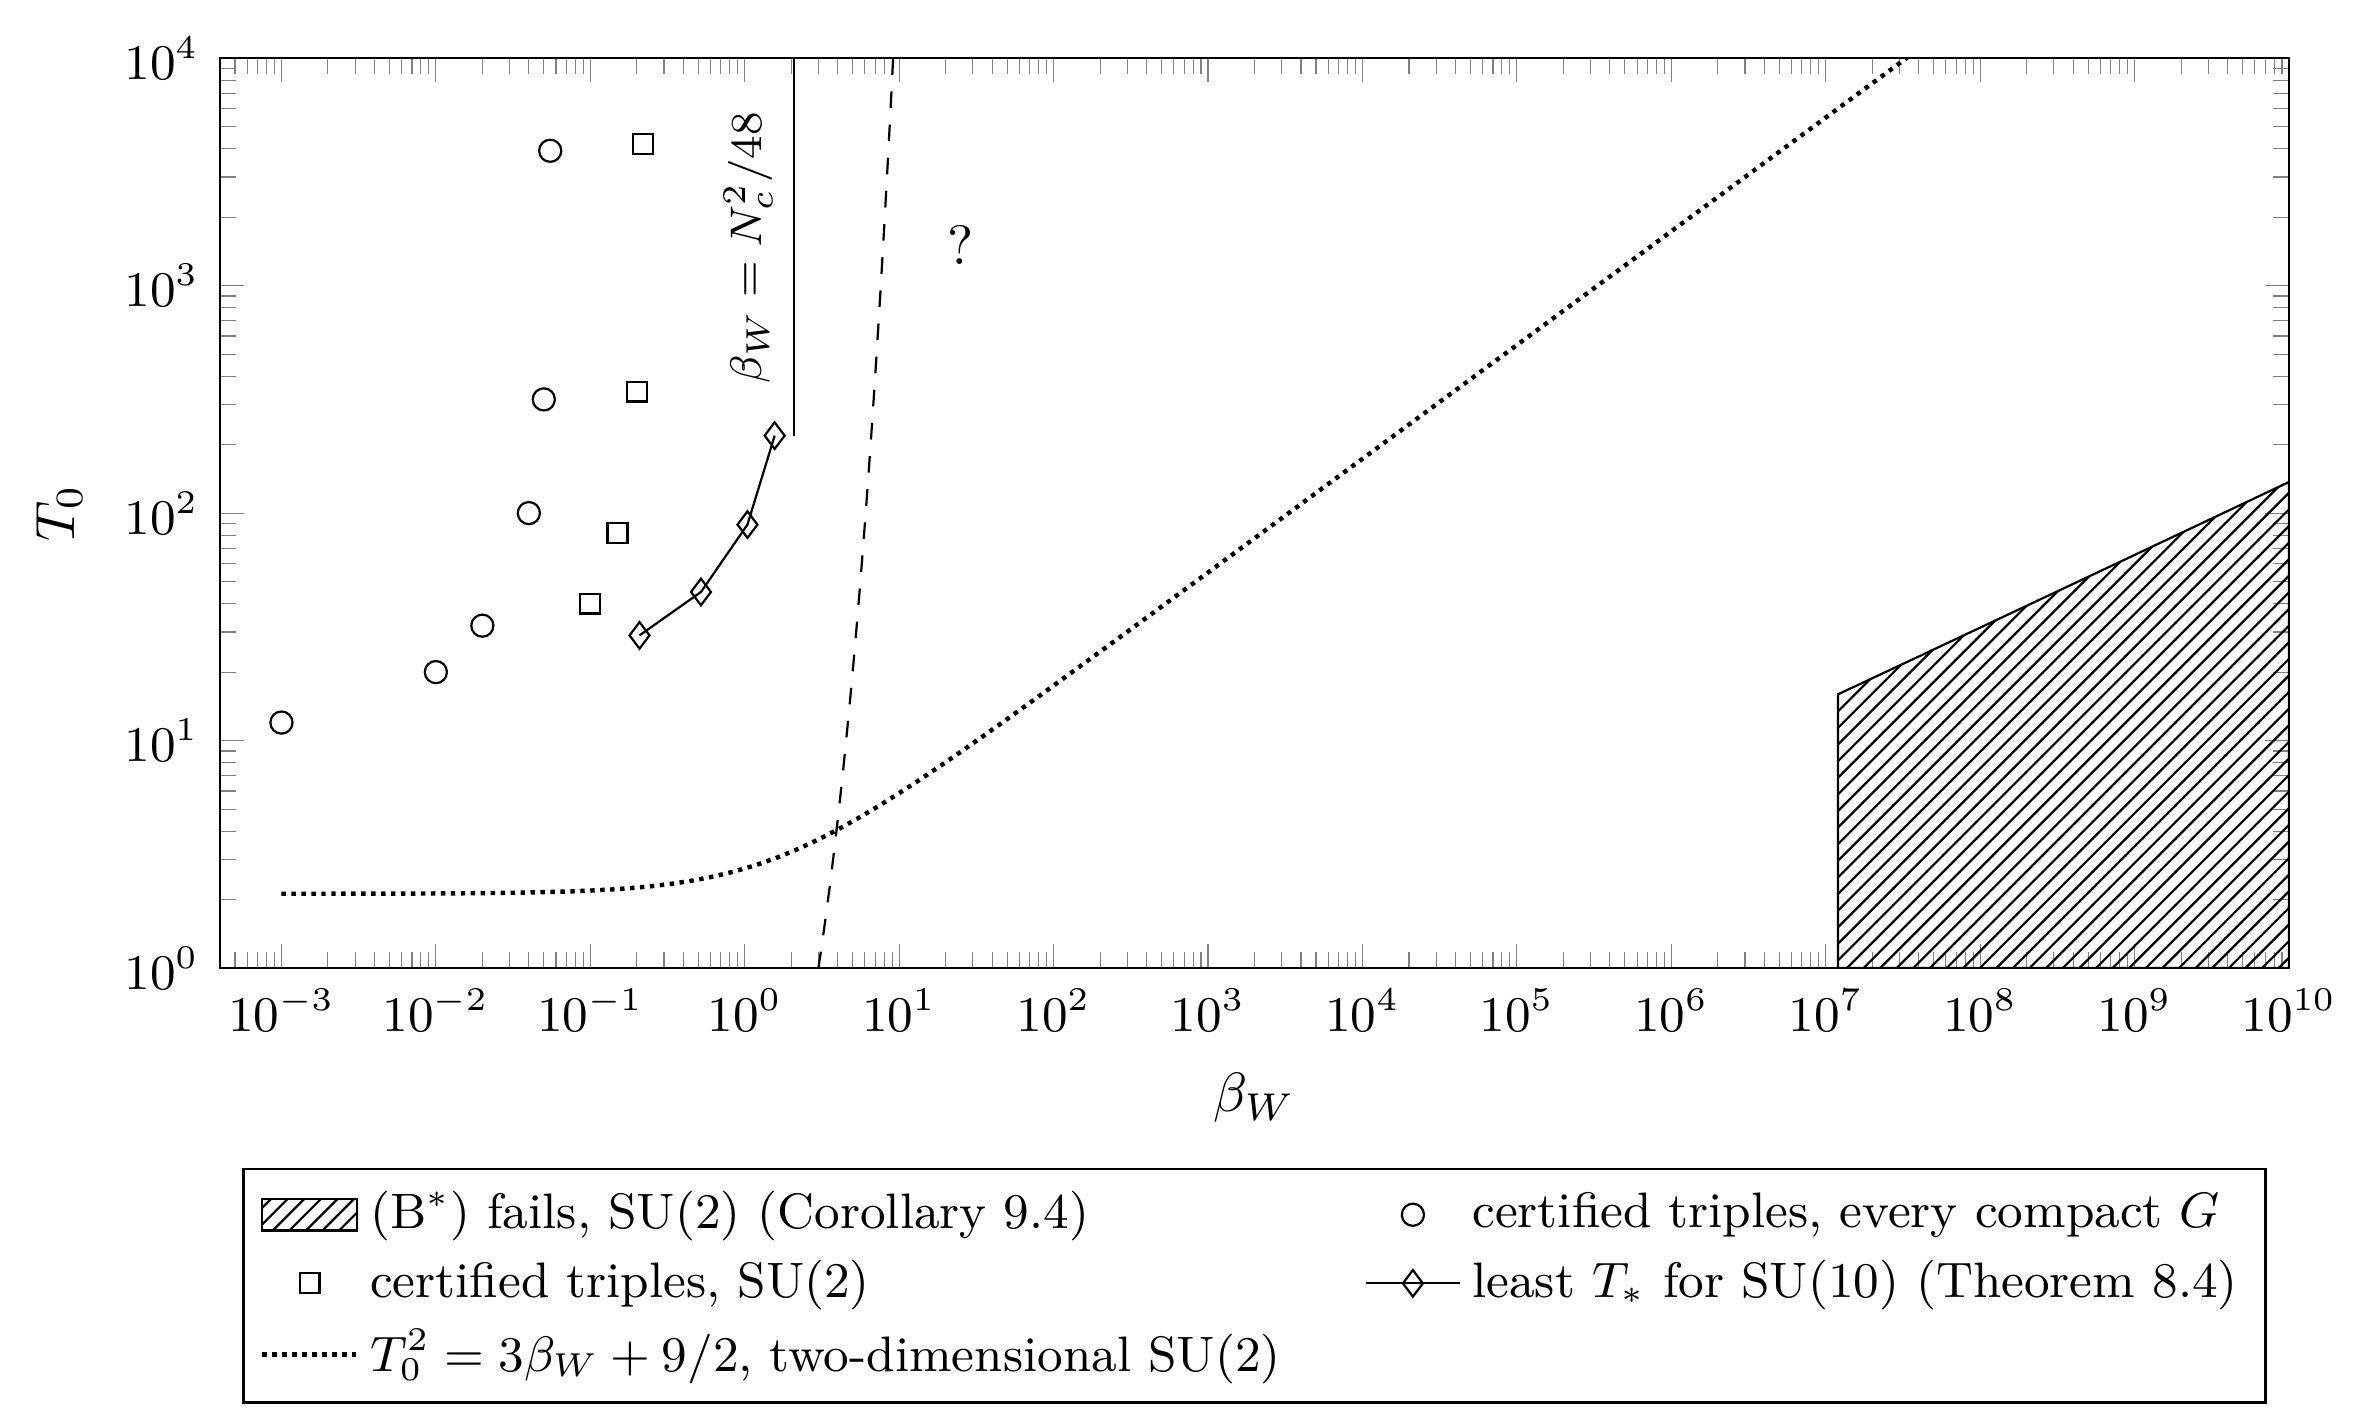
\includegraphics[width=427.2bp]{figures/fig12.png}
\caption{Where the datum is proved and where its window form \Bstar{} is excluded. Circles and squares: the certified triples $(\betaW,T_*)$ of \cref{tab:certified-triples}; at each the window inequality holds for every $\Tzero\ge T_*$ and every smaller coupling. Diamonds: the least $T_*$ of \cref{thm:large-N}\,(c) for $\SU(10)$; the vertical line is the end $\betaW=N_c^2/48$ of its range. Hatched: \Bstar{} fails for $\SU(2)$ by \cref{cor:base-scale}, drawn where that corollary applies ($\beta=\betaW/4\ge3\cdot10^6$). Dotted: the sufficient condition of \cref{thm:two-dim}\,(iv) for two-dimensional $\SU(2)$, a different theory. Dashed, schematic: the continuum tuning, along which the datum is not proved.}
\label{fig:datum-map}
\end{figure}

\subsection{Two dimensions}

Let $L,T\ge2$ be integers. The two-dimensional $\SU(2)$ Wilson theory on $(\Z/L)\times(\Z/T)$ has plaquette weight $f(U_p)$, $f(U)=\exp(\frac{\betaW}2\Tr U)=e^{\betaW\cos\vartheta}$, where $e^{\pm i\vartheta}$ are the eigenvalues of $U$; let $\Zpart{L}{T}$ be its partition function and $\psiT{L}{T}=2\log\Zpart{L}{T}-\log\Zpart{L}{2T}$. For an integer $\Tzero\ge3$ the two-dimensional datum\footnote{In dimension $n$ the threshold $\Vol{s}/(161(48\Tzero)^{n-1})$ is the only power of $\Tzero$ invariant under $(s,\Tzero)\mapsto(\lambda s,\lambda\Tzero)$, as a tuning with $\Tzero\simeq\tzero/a$ requires; for $n=4$ it is \eqref{ms:eq:rational-condition}. In two dimensions the window may be replaced by all $L\ge2\Tzero$, because $L=2\Tzero$ is binding (part (iv) below).} is
\begin{equation}\label{eq:2d-datum}
(\mathrm D_2)\qquad \psiT{L}{\Tzero}\le\frac{L}{161\cdot48\,\Tzero}\qquad\text{for every integer }L\ge2\Tzero .
\end{equation}
For $n\ge0$ let $I_n(x)=\frac1\pi\int_0^\pi e^{x\cos\vartheta}\cos n\vartheta\dd\vartheta$. Expanding the exponential and integrating by parts give
\begin{equation}\label{eq:2d-bessel}
I_n(x)=\sum_{j\ge0}\frac{(x/2)^{n+2j}}{j!\,(n+j)!},\qquad I_{n-1}-I_{n+1}=\frac{2n}{x}I_n,\qquad I_n'=\tfrac12(I_{n-1}+I_{n+1}).
\end{equation}
Put $\rho_n=I_n(\betaW)/I_1(\betaW)$, $\zeta(A)=\sum_{n\ge1}\rho_n^A$ and $\psi(A)=2\log\zeta(A)-\log\zeta(2A)$ for $A>0$, and
\[
h_-=\operatorname{arsinh}\frac{3}{2\betaW},\qquad h_+=\log\frac{3+\sqrt{4\betaW^2+25}}{2\betaW}.
\]

\begin{theorem}[two-dimensional $\SU(2)$ at every coupling]\label{thm:two-dim}
Let $\betaW>0$.
\begin{enumerate}[label=\textup{(\roman*)},leftmargin=*]
\item For all integers $L,T\ge2$, $\Zpart{L}{T}=\sum_{n\ge1}\bigl(2I_n(\betaW)/\betaW\bigr)^{LT}$ and $\psiT{L}{T}=\psi(LT)$.
\item For integers $\nu\ge0$ and $x>0$, $r_\nu=I_{\nu+1}/I_\nu$ satisfies
\begin{equation}\label{eq:2d-ratio}
\frac{x}{\nu+\frac12+\sqrt{(\nu+\frac32)^2+x^2}}<r_\nu(x)<\frac{x}{\nu+\frac12+\sqrt{(\nu+\frac12)^2+x^2}}=e^{-\operatorname{arsinh}\frac{\nu+1/2}{x}}.
\end{equation}
\item $\psi>0$ on $(0,\infty)$, and $\psi$ is strictly decreasing.
\item Let $\Tzero\ge3$. $(\mathrm D_2)$ holds if and only if $\psi(2\Tzero^2)\le1/3864$, and the set of integers $\Tzero\ge3$ at which it holds is $\{\Tzero\ge T_c(\betaW)\}$ for an integer $T_c(\betaW)\ge3$. It holds if $2\Tzero^2h_-\ge\log7729$, in particular if $\Tzero^2\ge3\betaW+\frac92$. It fails at $L=2\Tzero$ if $2\Tzero^2h_+\le\log7700$, in particular if $\Tzero^2\bigl(\frac3\betaW+\frac{25}{4\betaW^2}\bigr)\le8.948$.
\item Let $a\to0$ with $\betaW=4/(g^2a^2)$, $g>0$, and let $L,\Tzero$ be integers with $aL\to\ell>0$, $a\Tzero\to\tau>0$. Then $\psiT{L}{\Tzero}\to\psi_{\mathrm{cont}}(g^2\ell\tau)$, where $\psi_{\mathrm{cont}}(x)=2\log\Theta(x)-\log\Theta(2x)$ and $\Theta(x)=\sum_{n\ge1}e^{-(n^2-1)x/8}$. The function $\psi_{\mathrm{cont}}$ is strictly decreasing, and $\psi_{\mathrm{cont}}(2\kappa_c)=1/3864$ defines a unique $\kappa_c\in(11.936,11.937)$. For $\tzero>0$ and all sufficiently small $a$, $(\mathrm D_2)$ holds at $\Tzero=\lfloor\tzero/a\rfloor$ if $g^2\tzero^2>\kappa_c$, and fails at every integer $\Tzero\in[3,\tzero/a]$ if $g^2\tzero^2<\kappa_c$. The string tension $\sigma=-\log\rho_2$ satisfies $a^{-2}\sigma\to\sigma_{\mathrm{ph}}=\frac38g^2$, and $\tau_c=\sqrt{\kappa_c}/g$ satisfies $\tau_c\sqrt{\sigma_{\mathrm{ph}}}\in(2.1156,2.1158)$.
\end{enumerate}
\end{theorem}

\begin{proof}
(i) Let $\chi_n(U)=\sin n\vartheta/\sin\vartheta$ be the character of dimension $n$; by Weyl's formula, with Bessel functions evaluated at $\betaW$,
\[
c_n:=\int f\chi_n\dd U=\frac2\pi\int_0^\pi e^{\betaW\cos\vartheta}\sin n\vartheta\,\sin\vartheta\dd\vartheta=I_{n-1}-I_{n+1}=\frac{2n}{\betaW}I_n>0 .
\]
By \eqref{eq:2d-bessel}, $\sum_nnc_n<\infty$, so $f=\sum_nc_n\chi_n$ uniformly, and $\int\chi_m(W)\chi_n(W^{-1}Y)\dd W=\delta_{mn}\chi_n(Y)/n$ gives $\int f(W)\chi_n(W^{-1}Y)\dd W=(c_n/n)\chi_n(Y)$. The transfer operator on $L^2(\SU(2)^L)$, the spatial links $Q_1,\dots,Q_L$ of a slice, has kernel $K_L(Q,Q')=\int\prod_xf(Q_xU_{x+1}Q_x'^{*}U_x^{*})\prod_x\dd U_x$ ($U_{L+1}=U_1$), and $\Zpart{L}{T}=\Tr K_L^T$. For $\psi_n(Q)=\chi_n(Q_1\cdots Q_L)$, the Haar-preserving substitution $W_x=Q_xU_{x+1}Q_x'^*U_x^*$ telescopes the product, $Q'_1\cdots Q'_L=U_1^*(W_1^*Q_1)\cdots(W_L^*Q_L)U_1$, and $L$ convolutions give $K_L\psi_n=(c_n/n)^L\psi_n$. The $\psi_n$ are orthonormal. The kernel is gauge invariant in $Q$ and in $Q'$ (substitute $U_x\mapsto U_xg_x$), so $K_L$ vanishes on the orthogonal complement of the gauge-invariant functions; these are class functions of $Q_1\cdots Q_L$ (gauge to $(1,\dots,1,Q_1\cdots Q_L)$) and lie in the closed span of the $\psi_n$ by the Peter--Weyl theorem. Taking traces gives $\Zpart{L}{T}$; the factor $(2I_1/\betaW)^{LT}$ cancels in $\psi$.

(ii) By \eqref{eq:2d-bessel}, $I_\nu'=I_{\nu+1}+\frac\nu xI_\nu$ and $I_{\nu+1}'=I_\nu-\frac{\nu+1}{x}I_{\nu+1}$, so $r=r_\nu$ solves $r'=\Phi(x,r):=1-\frac{2c}{x}r-r^2$, $c=\nu+\frac12$, and $r=\frac{x}{2(\nu+1)}-\frac{x^3}{8(\nu+1)^2(\nu+2)}+O(x^5)$. For $c'\ge c$ and $w=x/(c+\Sigma)$, $\Sigma=\sqrt{c'^2+x^2}$, a direct computation gives
\[
\Phi(x,w)=\frac{c'^2-c^2}{(c+\Sigma)^2},\qquad w'=\frac{c+c'^2/\Sigma}{(c+\Sigma)^2}.
\]
\emph{Upper bound}, $c'=c$: $\Phi(x,w)=0<w'$ and $w-r=x(\frac1{2\nu+1}-\frac1{2\nu+2})+O(x^3)>0$ near $0$. At $x_1=\inf\{r\ge w\}$, if finite, $r=w$ and $(r-w)'\ge0$, whereas $(r-w)'(x_1)=-w'(x_1)<0$. \emph{Lower bound}, $c'=\nu+\frac32$: $c'^2-c^2-c=c'$, so $\Phi(x,w)-w'=c'(1-c'/\Sigma)/(c+\Sigma)^2>0$, and $w=\frac{x}{2(\nu+1)}-\frac{x^3}{8c'(\nu+1)^2}+O(x^5)$ gives $r-w>0$ near $0$ as $c'<\nu+2$; at $x_1=\inf\{r\le w\}$, if finite, $(r-w)'\le0$, a contradiction. The last identity in \eqref{eq:2d-ratio} is $\operatorname{arsinh}y=\log(y+\sqrt{1+y^2})$.

\emph{Consequences.} At $\nu=1$, $h_-<\sigma<h_+$. The upper bounds decrease in $\nu$, so $\rho_n=\prod_{k=1}^{n-1}r_k(\betaW)\le e^{-(n-1)h_-}$, with strict inequality for $n\ge2$. From $\operatorname{arsinh}y\ge y-y^3/6$, $\sqrt{1+v}\le1+v/2$, $\log(1+v)\le v$ and $\sum_{k=1}^{n-1}(k+\frac12)=\frac{n^2-1}2$,
\begin{equation}\label{eq:2d-rhon}
\Bigl\lvert-\log\rho_n-\frac{n^2-1}{2\betaW}\Bigr\rvert\le\sum_{k=1}^{n-1}\Bigl[\frac{(k+\frac32)^2}{2\betaW^2}+\frac{(k+\frac12)^3}{6\betaW^3}\Bigr],\qquad h_+\le\frac{3}{2\betaW}+\frac{25}{8\betaW^2}.
\end{equation}

(iii) Let $\sigma_n=-\log\rho_n$ ($\sigma_1=0<\sigma_2$) and $\langle\cdot\rangle_A$ the mean under the weights $\rho_n^A/\zeta(A)$. Termwise differentiation is justified by $\rho_n\le e^{-(n-1)h_-}$, and $\frac{\dd}{\dd A}\log\zeta=-\langle\sigma\rangle_A$, $\frac{\dd}{\dd A}\langle\sigma\rangle_A=-\Var_A(\sigma)<0$, so $\psi'(A)=2(\langle\sigma\rangle_{2A}-\langle\sigma\rangle_A)<0$. Positivity is $\zeta(2A)<\zeta(A)^2$.

(iv) $\psiT{L}{\Tzero}=\psi(L\Tzero)$ decreases in $L$ and the threshold increases, so $L=2\Tzero$ is binding, with threshold $2/7728=1/3864$. The condition is upward closed in $\Tzero$ by (iii) and holds for large $\Tzero$, since $\psi(A)\le2\log\zeta(A)\to0$. \emph{Sufficiency}: with $A=2\Tzero^2$, $\psi(A)\le2\log\zeta(A)\le2(\zeta(A)-1)<2(e^{Ah_-}-1)^{-1}\le2/7728$ if $e^{Ah_-}\ge7729$; and $h_-\ge3/\sqrt{4\betaW^2+9}\ge3/(2\betaW+3)$ (from $\operatorname{arsinh}y\ge y/\sqrt{1+y^2}$), so $\Tzero^2\ge\frac32(2\betaW+3)$ gives $2\Tzero^2h_-\ge9$, and $e^9>7729$. \emph{Failure}: let $\varepsilon=\zeta(A)-1>e^{-Ah_+}$; then $\zeta(2A)-1\le\varepsilon^2$ and $\zeta(2A)\le\zeta(A)$, so $\psi(A)\ge\log\zeta(A)\ge\log2$ if $\varepsilon\ge1$, and $\psi(A)\ge\phi(\varepsilon)=2\log(1+\varepsilon)-\log(1+\varepsilon^2)$ if $\varepsilon\le1$. On $[0,1]$, $\phi$ increases ($\phi'=2(1-\varepsilon)/((1+\varepsilon)(1+\varepsilon^2))$) and $\phi(\varepsilon)\ge2\varepsilon-2\varepsilon^2$. If $Ah_+\le\log7700$, then $\varepsilon>1/7700$ and $\psi(A)>\min\{\log2,\,2/7700-2/7700^2\}>1/3864$, as $15398\cdot3864=59497872>7700^2$. The explicit form uses \eqref{eq:2d-rhon} and $\log7700>8.948$.

(v) Let $A=L\Tzero$, $x=g^2\ell\tau$ and $y=3/(2\betaW)=\frac38g^2a^2$. Then $A/(2\betaW)\to x/8$ and $A/\betaW^2\to0$, so $A\sigma_n\to(n^2-1)x/8$ by \eqref{eq:2d-rhon}; and $\rho_n^A\le e^{-(n-1)Ah_-}$ with $Ah_-\ge A(y-y^3/6)\to3x/8>0$, so dominated convergence gives $\zeta(A)\to\Theta(x)$, $\zeta(2A)\to\Theta(2x)$. The argument of (iii) with $\sigma_n=(n^2-1)/8$ shows that $\psi_{\mathrm{cont}}$ is strictly decreasing. Exact rational arithmetic with Taylor remainders and $1+e^{-3x/8}\le\Theta(x)\le1+e^{-3x/8}+e^{-x}/(1-e^{-x/2})$, which uses $(n^2-1)/8\ge(n-1)/2$ for $n\ge3$, gives $\psi_{\mathrm{cont}}(23.872)>1/3864>\psi_{\mathrm{cont}}(23.874)$ (\cref{app:certificates}); hence $2\kappa_c\in(23.872,23.874)$. For $3\le\Tzero\le\lfloor\tzero/a\rfloor$, (iii) gives $\psi(2\Tzero^2)\ge\psi(2\lfloor\tzero/a\rfloor^2)$, and the limit with $L=2\lfloor\tzero/a\rfloor$ gives $\psi(2\lfloor\tzero/a\rfloor^2)\to\psi_{\mathrm{cont}}(2g^2\tzero^2)$, below $1/3864$ if $g^2\tzero^2>\kappa_c$ and above it if $g^2\tzero^2<\kappa_c$; (iv) gives both statements. Finally $h_-<\sigma<h_+$ with $a^{-2}h_-\ge a^{-2}(y-y^3/6)\to\frac38g^2$ and, by \eqref{eq:2d-rhon}, $a^{-2}h_+\to\frac38g^2$; and $\sqrt{3\kappa_c/8}\in(2.1156,2.1158)$.
\end{proof}

At finite $a$ the boundary case $g^2\tzero^2=\kappa_c$ is not decided. Explicit criteria follow from (iv) and $\operatorname{arsinh}y\ge y-y^3/6$: with $\tau=a\Tzero$, $(\mathrm D_2)$ holds at $\Tzero$ if $\frac34g^2\tau^2(1-\frac3{128}g^4a^4)\ge8.953$ $(>\log7729)$ and fails if $\tau^2(\frac34g^2+\frac{25}{64}g^4a^2)\le8.948$; so for small $a$ it holds at $\lfloor\tzero/a\rfloor$ when $g^2\tzero^2>11.9374$ and fails at every integer $\Tzero\in[3,\tzero/a]$ when $g^2\tzero^2<11.9306$, a bracket around $\kappa_c$. The ratio bounds (ii) are classical \cite{amos1974,segura2011}. Part (i) is the case $G=\SU(2)$ of \cite[Prop.~A5(i)]{bhattacharjee2026first}, and \eqref{eq:2d-rhon} is a variant of the bounds of \cite[Prop.~A5(ii)]{bhattacharjee2026first}; parts (ii)--(v) and the threshold $1/3864$ are not in the first paper, which bounds the two-dimensional pressure with an implicit constant \cite[Prop.~25]{bhattacharjee2026first}. The two-dimensional theory has no propagating gluons, and \cref{thm:two-dim} has no bearing on the four-dimensional datum, which forces a gap on the box of side $2\Tzero$ in three and four dimensions (\cref{prop:finite-volume-gap}).
\section{Necessary conditions on any proof}\label{sec:necessary}

This section lists what every proof of \Mcirc{} has to accomplish. Each statement is a proved theorem about the Wilson theory or about every \PSTS; none of them proves \Mcirc.

The statements fall into three groups. On a fixed torus the gap of the Wilson transfer matrix tends to zero as the coupling grows (\cref{thm:fixed-torus-gap,thm:SUN-gap}). Hence the base scale grows at least like $(\beta/\log\beta)^{1/3}$ (\cref{cor:base-scale}), no fixed window and no expansion that is uniform in the volume carries the datum (\cref{thm:fixed-window}), and the flux residue saturates (\cref{prop:flux-saturation}). On the cube of the datum, \Mcirc{} forces a gap $T(E_1-E_0)>9.01$ and nearly free twists (\cref{prop:spectral-conditions}). The free-gluon reference $\Gharm$ violates these conditions by a factor that does not depend on the scale, in every real symmetry sector, and the passage to $\SU(N)/\Z_N$ does not remove the obstruction (\cref{prop:no-stefan-boltzmann,thm:free-gluon,thm:pair,thm:exclusivity}). Finally, the window datum forces a large gap in a small box in every dimension (\cref{prop:finite-volume-gap}), while a gap bounded below in lattice units, or a spatially finite correlation length together with one rotation, forces a trivial continuum limit (\cref{prop:lattice-unit-triviality,thm:rotation-triviality}).

\medskip\noindent\textit{Conventions.} For a \PSTS{} and $T\ge2$, \Bcirc{} at $T$ means $\XT{\cube{T}}{T}\le\xconst$ (\cref{eq:datum-B}). By \cref{lem:purity-conversion}, \Mcirc{} at $T$ implies \Bcirc{} at $T$, so every consequence of \Bcirc{} proved below is a necessary condition for \Mcirc. The window datum \cref{ms:eq:rational-condition} at $T_0$ reads $\psiT{s}{T_0}\le\Vol{s}/(161(48T_0)^3)$ for all $s\in\Wwin_{T_0}=\{s:2T_0\le s_j<48T_0\}$.

For $G=\SU(N)$ the Wilson weight is $\exp(b\sum_p\ReTr Q_p)$ with $b=N\beta$ and $\betaW=Nb$, and $A_p=N-\ReTr Q_p=\frac12\norm{Q_p-1}_F^2$. For $\SU(2)$ we write $c=b=2\beta$, so that $\betaW=4\beta=2c$, and
\[
\varepsilon(c)=\frac{12(\log c+5.42)}{c}.
\]
For a spatial torus $t=(\ell_1,\ell_2,\ell_3)$ let $\mu_{t,M}$ be the Wilson measure on $t\times\Z_M$, $\mu^0_t=\lim_M\mu_{t,M}$ its slice limit, $R=\TT_t/\lzero$ and $r_1(t)=\lambda_1/\lzero$ (\cref{lem:transfer-matrix}). Eigenvectors of $\TT_t$ with nonzero eigenvalue are gauge invariant \cite[Lemma~11(i)]{bhattacharjee2026first}, so $R\le r_1$ on $\Omegazero^\perp$. For bounded functions $F,G$ of the slice at time $0$ one has $\ip{F\Omegazero}{R^sG\Omegazero}=\mu^0_t(\bar F\,\tau_sG)$, with $\tau_s$ the time translation, and bounds on $\mu_{t,M}$ that are uniform in $M$ pass to $\mu^0_t$ \cite[Lemma~11(v)]{bhattacharjee2026first}. With time-translation invariance this gives the Dirichlet identity
\[
\ip{F\Omegazero}{(1-R)F\Omegazero}=\tfrac12\,\mu^0_t\bigl(\abs{F-\tau_1F}^2\bigr),
\]
valid also for complex $F$ because the left side is real \cite[Theorem~8, Step~4]{bhattacharjee2026first}.

\subsection{Three holonomies and the gap on a fixed torus}

\begin{lemma}[Lemma W]\label{lem:lemma-W}
For $P=(P_1,P_2,P_3)\in\SU(2)^3$ put
\begin{multline*}
\Phi(P)=\frac14\sum_{i=1}^3(\Tr P_i)^2+\frac16\sum_{i<j}\bigl[(\Tr P_iP_j)^2+(\Tr P_iP_j^{-1})^2\bigr]\\
+\frac18\bigl[(\Tr P_1P_2P_3)^2+(\Tr P_1^{-1}P_2^{-1}P_3^{-1})^2\bigr].
\end{multline*}
Then $\Phi\ge1$ on $\SU(2)^3$. Equality holds at $(i\sigma_1,i\sigma_2,i\sigma_3)$, at $(1,i\sigma_1,i\sigma_2)$, and at $(in_1\cdot\sigma,in_2\cdot\sigma,in_3\cdot\sigma)$ for coplanar unit vectors $n_1,n_2,n_3$ at mutual angles $2\pi/3$, and along the curve $(\cos\theta+i\sin\theta\,\sigma_3,i\sigma_1,i\sigma_2)$, which joins the second configuration to a permutation of the first; \cref{app:lemma-W} describes the whole equality set.
\end{lemma}

The eleven words of $\Phi$ are the charged words of \cref{fig:holonomies}: each has an odd exponent sum in at least one holonomy.

\begin{proof}
Write $P_k=a_k+ib_k\cdot\sigma$ with $a_k\in\R$, $b_k\in\R^3$, $a_k^2+\abs{b_k}^2=1$, and put $g_{ij}=b_i\cdot b_j$, $A=\sum_ka_k^2$, $S=\sum_{i<j}g_{ij}^2$, $s=a_1a_2a_3-a_1g_{23}-a_2g_{13}-a_3g_{12}$ and $d=\det(b_1,b_2,b_3)$. From $(iu\cdot\sigma)(iv\cdot\sigma)=-u\cdot v-i(u\times v)\cdot\sigma$ one obtains (\cref{app:lemma-W})
\begin{gather*}
\Tr P_k=2a_k,\qquad\Tr P_iP_j^{\pm1}=2(a_ia_j\mp g_{ij}),\\
\Tr P_1P_2P_3=2(s+d),\qquad\Tr P_3P_2P_1=2(s-d),
\end{gather*}
and $\Tr P_1^{-1}P_2^{-1}P_3^{-1}=\Tr P_3P_2P_1$ because traces in $\SU(2)$ are real. Summing the squares with the weights of $\Phi$,
\[
\Phi=A+\tfrac43\sum_{i<j}a_i^2a_j^2+\tfrac43S+s^2+d^2\ \ge\ A+\tfrac43S+\det\mathsf{Gr},
\]
where $\mathsf{Gr}$ is the Gram matrix of $b_1,b_2,b_3$, so that $d^2=\det\mathsf{Gr}$. With $p_k=\abs{b_k}^2=1-a_k^2\in[0,1]$,
\[
\det\mathsf{Gr}=p_1p_2p_3+2g_{12}g_{13}g_{23}-p_1g_{23}^2-p_2g_{13}^2-p_3g_{12}^2\ \ge\ 1-A-\kappa(S),
\]
where $\kappa(S)=S+2(S/3)^{3/2}$, by $\prod_k(1-a_k^2)\ge1-A$, by $\abs{g_{12}g_{13}g_{23}}\le(S/3)^{3/2}$ (arithmetic and geometric means) and by $p_k\le1$. The function $\kappa$ is increasing and $\kappa(3/4)=1$. Hence $\Phi\ge h:=A+\frac43S+\max\{0,1-A-\kappa(S)\}$. If $S\ge3/4$ then $h\ge\frac43S\ge1$. If $A+\kappa(S)\le1$ then $S\le3/4$ and $h=1+\frac S3-2(\frac S3)^{3/2}$. If $A+\kappa(S)>1$ and $S<3/4$ then $h\ge A+\frac43S>1-\kappa(S)+\frac43S$, the same expression. For $0\le S\le3/4$ one has $(S/3)^{1/2}\le\frac12$, so $1+\frac S3\bigl(1-2(S/3)^{1/2}\bigr)\ge1$. At the three configurations of the statement $(A,S,s,d)$ equals $(0,0,0,\pm1)$, $(1,0,0,0)$ and $(0,\frac34,0,0)$, and $\Phi=1$ there.
\end{proof}

Three holonomies are needed. At $(P_1,P_2)=(i\sigma_1,i\sigma_2)$ the generated group is the quaternion group, and every word that is odd in $P_1$ or in $P_2$ is mapped to some $\pm i\sigma_k$ and is traceless. So the charged traces of two holonomies have common zeros; this is why \cite[Theorem~8]{bhattacharjee2026first} needs the flatness condition $(\ell_1\ell_2)^2\varepsilon(c)<3$. The third holonomy removes it.

\begin{theorem}[the gap on a fixed torus tends to zero]\label{thm:fixed-torus-gap}
Let $G=\SU(2)$ and $c=2\beta\ge\frac1{32}$. Every spatial torus $t=(\ell_1,\ell_2,\ell_3)$ with all sides $\ge3$ satisfies
\[
1-r_1(t)\le\varepsilon(c)\Bigl[\tfrac12\sum_i\ell_i^2+\tfrac23\sum_{i<j}(\ell_i+\ell_j)^2+\tfrac12(\ell_1+\ell_2+\ell_3)^2\Bigr]\le\tfrac{14}{3}\,(\ell_1^2+\ell_2^2+\ell_3^2)\,\varepsilon(c).
\]
On the cube of side $\ell$ this reads $1-r_1\le14\,\ell^2\varepsilon(c)$.
\end{theorem}

\begin{proof}
\emph{Energy.} By \cite[Theorem~8, Step~1]{bhattacharjee2026first} (restated in \cref{app:first-paper}), $\mu^0_t(A_p)\le\varepsilon(c)$ for every plaquette $p$ of $t\times\Z$.

\emph{Charged words.} In the slice at time $0$ let $P_j$ be the ordered product of the links from the origin once around direction $j$. For each of the eleven words $W$ of \cref{lem:lemma-W} put $F_W=\Tr W(P_1,P_2,P_3)$; it is real, continuous and gauge invariant, being the trace of a closed loop at the origin. The centre flip $z_j$, which replaces $Q_{(x,j)}$ by $-Q_{(x,j)}$ on all links in direction $j$ with $x_j=0$, at all times, preserves Haar measure and every plaquette variable, since a plaquette contains none or two flipped links; so it preserves $\mu_{t,M}$ and $\mu^0_t$ \cite[Theorem~8, Step~2]{bhattacharjee2026first}. It maps $P_j\mapsto-P_j$ and fixes $P_i$ for $i\ne j$. Every letter that occurs in one of the eleven words occurs exactly once, so $z_jF_W=-F_W$ for some $j$; hence $\mu^0_t(F_W)=0$ and $F_W\Omegazero\perp\Omegazero$.

\emph{Dirichlet form.} The loop of $W$ has $m_W$ steps: $m_W=\ell_i$ for $P_i$, $m_W=\ell_i+\ell_j$ for $P_iP_j^{\pm1}$, and $m_W=\ell_1+\ell_2+\ell_3$ for the two triple words. Let $e_1,\dots,e_m$ be its links at time $0$, $e'_1,\dots,e'_m$ the corresponding links at time $1$, $x_0=0,x_1,\dots,x_m=0$ its sites and $u_x$ the temporal link at $x$. Put $X=e_1\cdots e_m$, $Y=u_{x_0}e'_1\cdots e'_mu_{x_0}^{-1}$ and
\[
X_k=e_1\cdots e_k\,u_{x_k}\,e'_{k+1}\cdots e'_m\,u_{x_0}^{-1},\qquad0\le k\le m.
\]
Then $X_0=Y$, $X_m=X$ and $X_k-X_{k-1}=V_k(Q_k-1)V'_k$ with $V_k,V'_k$ unitary and $Q_k=e_ku_{x_k}e_k'^{-1}u_{x_{k-1}}^{-1}$ the temporal plaquette of step $k$. Hence $\norm{X-Y}_F\le\sum_k\norm{Q_k-1}_F$. Since $F_W-\tau_1F_W=\Tr X-\Tr Y$, the bound $\abs{\Tr X-\Tr Y}\le\sqrt2\norm{X-Y}_F$ and Cauchy--Schwarz give
\[
(F_W-\tau_1F_W)^2\le2m_W\sum_k\norm{Q_k-1}_F^2=4m_W\sum_kA_{Q_k},
\]
and the Dirichlet identity gives $\ip{F_W\Omegazero}{(1-R)F_W\Omegazero}\le2m_W^2\varepsilon(c)$.

\emph{Combination.} Since $R\le r_1$ on $\Omegazero^\perp$ and $\norm{F_W\Omegazero}^2=\mu^0_t(F_W^2)$, the weights $w_W\in\{\frac14,\frac16,\frac18\}$ of $\Phi$ give
\[
(1-r_1)\,\mu^0_t(\Phi(P_1,P_2,P_3))\le\sum_Ww_W\ip{F_W\Omegazero}{(1-R)F_W\Omegazero}\le2\varepsilon(c)\sum_Ww_Wm_W^2 .
\]
By \cref{lem:lemma-W} the left factor $\mu^0_t(\Phi)$ is at least $1$, and $2\sum_Ww_Wm_W^2$ is the bracket in the statement. Finally $(\ell_i+\ell_j)^2\le2(\ell_i^2+\ell_j^2)$ and $(\sum_i\ell_i)^2\le3\sum_i\ell_i^2$ give the constant $\frac12+\frac23\cdot4+\frac32=\frac{14}3$; on cubes the bracket equals $14\ell^2$.
\end{proof}

For comparison, \cite[Theorem~8]{bhattacharjee2026first} gives $1-r_1\le2(\ell_1+\ell_2)^2\varepsilon(c)/(1-(\ell_1\ell_2)^2\varepsilon(c)/3)$, and only while $(\ell_1\ell_2)^2\varepsilon(c)<3$. \Cref{thm:fixed-torus-gap} holds on every torus with sides $\ge3$.

For $\SU(N)$ put $n=N^2-1$, let $\omega_n$ be the volume of the unit ball of $\R^n$, let $\operatorname{vol}(\SU(N))$ be the Riemannian volume for the metric $\norm{X}_F$ on $\mathfrak{su}(N)$, and
\[
c_N=\frac{0.94^n\,\omega_n}{\operatorname{vol}(\SU(N))},\qquad\varepsilon_N(b)=\frac2b\Bigl[6+4\log\frac1{c_N}+2n\log(8b)\Bigr].
\]
For a word $W$ in $P_1^{\pm1},P_2^{\pm1},P_3^{\pm1}$ let $n(W)\in\Z^3$ be its exponent-sum vector, $\abs W$ its length, and $m_W(t)=\sum\ell_{j}$, the sum over the letters of $W$ with $j$ the direction of the letter.

\begin{theorem}[$\SU(N)$]\label{thm:SUN-gap}
Let $G=\SU(N)$, $N\ge2$, $t$ a spatial torus with sides $\ell_i\ge3$, and $\varepsilon\ge\sup_p\mu^0_t(A_p)$.
\begin{enumerate}[label=\textup{(\alph*)},leftmargin=*]
\item For $b\ge\frac12$ one may take $\varepsilon=\varepsilon_N(b)$. For $\SU(2)$, $\varepsilon_2(b)\le\frac{12}b(\log b+4.931)$.
\item There are a finite set $\mathcal W$ of words with $n(W)\not\equiv0\pmod N$ and a constant $\gamma_N>0$ such that
\[
1-r_1(t)\le\frac N{\gamma_N}\,\varepsilon\sum_{W\in\mathcal W}m_W(t)^2\le K_N\,\ell_{\max}^2\,\varepsilon,\qquad K_N=\frac N{\gamma_N}\sum_{W\in\mathcal W}\abs W^2 .
\]
\item There is $\kappa_N\in(0,2\sqrt N\sin(\pi/N)]$, and $\kappa_2=\sqrt2$ is admissible, such that $2(\ell_1\ell_2)^2\varepsilon<\kappa_N^2$ implies
\[
1-r_1(t)\le\frac{2(N-1)(N^2-1)(\ell_1+\ell_2)^2\,\varepsilon}{N\bigl(1-2(\ell_1\ell_2)^2\varepsilon/\kappa_N^2\bigr)} .
\]
\end{enumerate}
\end{theorem}

\begin{proof}
(a) Fix a periodic four-dimensional lattice with $\abs\Lambda$ sites, $4\abs\Lambda$ links and $6\abs\Lambda$ plaquettes, let $A=\sum_pA_p$ and $\tilde Z(b)=\int e^{-bA}\prod_e\dd Q_e\le1$ with Haar probability measure, so that the Wilson mean of $A$ is $\mathbb E_b[A]=-(\log\tilde Z)'(b)$. This mean is nonincreasing in $b$, since $(\log\tilde Z)''=\Var_b(A)\ge0$; hence
\[
\tfrac b2\,\mathbb E_b[A]\le\int_{b/2}^b\mathbb E_{b'}[A]\dd b'=\log\tilde Z(b/2)-\log\tilde Z(b)\le-\log\tilde Z(b).
\]
If $\norm{Q_e-1}_F\le r$ on every link, then $\norm{Q_p-1}_F\le4r$ and $A_p\le8r^2$. Take $r^2=1/(8b)$; then $A_p\le1/b$, and $r\le\frac12$ because $b\ge\frac12$. The chord ball $\{\norm{Q-1}_F\le r\}$ contains $\exp\{X\in\mathfrak{su}(N):\norm X_F\le r\}$, because $\norm{e^X-1}_F\le\norm X_F$. In exponential coordinates the Haar density is $\operatorname{vol}(\SU(N))^{-1}\prod_{\alpha>0}\bigl(\sin(\alpha(X)/2)/(\alpha(X)/2)\bigr)^2$; since $\abs{\alpha(X)}\le2\norm X_F$ and $\sin y/y\ge1-y^2/6$, each factor is at least $(1-0.58^2/6)^2>0.94^2$ for $\norm X_F\le0.58$, and there are $N(N-1)/2\le n/2$ positive roots. As $\exp$ is injective on $\norm X_F<\pi$, the ball has Haar measure at least $c_Nr^n$. Restricting the integral to the product of these balls,
\[
\tilde Z(b)\ge e^{-6\abs\Lambda}\bigl(c_Nr^n\bigr)^{4\abs\Lambda},\qquad\mathbb E_b[A]\le\frac2b\,\abs\Lambda\Bigl[6+4\log\frac1{c_N}+2n\log(8b)\Bigr]=\abs\Lambda\,\varepsilon_N(b).
\]
The $\abs\Lambda$ translates of a plaquette have equal expectation and $A_p\ge0$, so $\mathbb E_b[A_p]\le\varepsilon_N(b)$ on every lattice, and the bound passes to $\mu^0_t$. For $\SU(2)$, $\operatorname{vol}(\SU(2))=4\sqrt2\pi^2$ and $\omega_3=4\pi/3$ give $1/c_2<16.05$, and $1+\frac23\log16.05+\log8<4.931$.

(b) First, the charged traces have no common zero. Suppose $\Tr W(P)=0$ for every word with $n(W)\not\equiv0\pmod N$, and let $\omega=e^{2\pi i/N}$. The unitary representations $\rho(x_i)=P_i$ and $\rho_j(x_i)=\omega^{\delta_{ij}}P_i$ of the free group on three generators then have equal traces, since $\Tr\rho_j(W)=\omega^{n_j(W)}\Tr\rho(W)$; two unitary representations with equal traces are equivalent, so there are $g_j$ with $g_jP_jg_j^{-1}=\omega P_j$ and $g_jP_ig_j^{-1}=P_i$ for $i\ne j$. The spectrum of $P_1$ is invariant under multiplication by $\omega$, hence is one orbit with $N$ distinct eigenvalues, and $g_1$ is a weighted cyclic shift of the eigenvectors with $N$ distinct eigenvalues. Its centraliser is commutative and contains $P_2,P_3$; so $P_2P_3=P_3P_2$, and likewise all $P_i$ commute. Their joint spectrum, $N$ points with multiplicity, is invariant under the free action of $\Z_N^3$ by phases, whose orbits have $N^3>N$ points, a contradiction. By compactness of $\SU(N)^3$ a finite family $\mathcal W$ of charged words has no common zero, and $\Phi_{\mathcal W}=\sum_{W\in\mathcal W}\abs{\Tr W}^2$ has a positive minimum $\gamma_N$ (the details are in \cref{app:lemma-W}). Now repeat the proof of \cref{thm:fixed-torus-gap} with $F=\operatorname{Re}\Tr W$ and $F=\operatorname{Im}\Tr W$. The map $z_j\colon Q_{(x,j)}\mapsto\omega Q_{(x,j)}$ on the links in direction $j$ with $x_j=0$ preserves the measure, since a plaquette contains none of these links or two with opposite orientations, and multiplies $\Tr W$ by $\omega^{n_j(W)}$; so $\mu^0_t(\Tr W)=0$. The Dirichlet forms of the real and imaginary parts sum to $\frac12\mu^0_t\abs{\Tr X-\Tr Y}^2\le\frac N2\mu^0_t\bigl((\sum_k\norm{Q_k-1}_F)^2\bigr)\le Nm_W^2\varepsilon$, by $\abs{\Tr Z}\le\sqrt N\norm Z_F$ and $\norm{Q-1}_F^2=2A_Q$, and their second moments sum to $\mu^0_t\abs{\Tr W}^2$. Hence $(1-r_1)\gamma_N\le(1-r_1)\mu^0_t(\Phi_{\mathcal W})\le N\varepsilon\sum_Wm_W^2$, and $m_W\le\abs W\ell_{\max}$.

(c) \emph{Trial functions.} Let $P_1,P_2$ be the slice-$0$ loops through the origin in directions $1,2$, and for $m\in\mathcal M=\{m\in\Z^2:0<\max_i\abs{m_i}\le N-1\}$ put $F_m=\Tr(P_1^{m_1}P_2^{m_2})$. The centre maps $z_1,z_2$ multiply $F_m$ by $\omega^{m_1}$ and $\omega^{m_2}$, and some $m_i\notin N\Z$, so $F_m\Omegazero\perp\Omegazero$. For weights $w_m\ge0$,
\[
1-r_1\le\frac{\sum_mw_m\ip{F_m\Omegazero}{(1-R)F_m\Omegazero}}{\sum_mw_m\,\mu^0_t(\abs{F_m}^2)} .
\]
\emph{Fej\'er weights.} Take $w_m=a_{m_1}a_{m_2}$ with $a_k=(1-\abs k/N)_+$, so that $\sum_{m\in\Z^2}w_m=N^2$ and $\sum_{\mathcal M}w_m=N^2-1$. Since $\abs{\Tr X}^2=\Tr_{M_N}(\operatorname{Ad}X)$,
\[
Q:=\sum_{m\in\Z^2}w_m\abs{\Tr(P_1^{m_1}P_2^{m_2})}^2=\Tr_{M_N}\bigl(\mathbb F(\operatorname{Ad}P_1)\,\mathbb F(\operatorname{Ad}P_2)\bigr),\qquad\mathbb F(e^{i\theta})=\sum_ka_ke^{ik\theta}\ge0,
\]
a trace of a product of two positive operators, so $Q\ge0$. If $P_1P_2=P_2P_1$, both $\operatorname{Ad}P_i$ fix the $N$ diagonal matrix units, on which $\mathbb F=N$, so $Q\ge N^3$. Hence $Q'=Q-N^2=\sum_{\mathcal M}w_m\abs{F_m}^2$ is $\ge0$, and $\ge N^2(N-1)$ when $P_1,P_2$ commute.

\emph{Compactness.} The set $\{(A,B)\in\SU(N)^2:Q'\le N^2(N-1)/2\}$ is compact and disjoint from the commuting pairs, on which $k(A,B)=\norm{ABA^{-1}B^{-1}-1}_F$ vanishes. So $\kappa_N=\min k$ over it is positive, and $k<\kappa_N$ implies $Q'>N^2(N-1)/2$. The clock and shift matrices (times a phase if $N$ is even) lie in this set, since $\Tr(C^{m_1}S^{m_2})=0$ on $\mathcal M$, and their commutator is a scalar $\omega^{\pm1}$; hence $\kappa_N\le\sqrt N\abs{\omega-1}=2\sqrt N\sin(\pi/N)$. For $\SU(2)$ write $x=\Tr A$, $y=\Tr B$, $z=\Tr AB$, $w=\Tr AB^{-1}$; then $Q'=x^2+y^2+\frac12(z^2+w^2)$. Fricke's bound $x^2+y^2+z^2\ge3-\eta$, $\eta=2-\Tr ABA^{-1}B^{-1}$ \cite[Theorem~8, Step~3]{bhattacharjee2026first}, applies to $(A,B)$ and to $(A,B^{-1})$, whose commutators have the same trace; so $Q'\ge3-\eta=3-\frac12\norm{ABA^{-1}B^{-1}-1}_F^2$, and $k<\sqrt2$ gives $Q'>2$.

\emph{Denominator.} $K=P_1P_2P_1^{-1}P_2^{-1}$ is the boundary holonomy of the sheet of the $\ell_1\ell_2$ plaquettes of the $(1,2)$-plane through the origin, so $\norm{K-1}_F\le\sum_{\text{sheet}}\norm{U_p-1}_F$ \cite[Theorem~8, Step~3]{bhattacharjee2026first}. Then $\norm{K-1}_F^2\le2\ell_1\ell_2\sum_{\text{sheet}}A_p$ and $\mu^0_t\norm{K-1}_F^2\le2(\ell_1\ell_2)^2\varepsilon$. By Chebyshev's inequality and $Q'\ge0$, $\mu^0_t(Q')\ge\frac12N^2(N-1)\bigl(1-2(\ell_1\ell_2)^2\varepsilon/\kappa_N^2\bigr)$.

\emph{Numerator.} The loop of $F_m$ has $M_m=\abs{m_1}\ell_1+\abs{m_2}\ell_2\le(N-1)(\ell_1+\ell_2)$ steps, and the strip interpolation of the proof of \cref{thm:fixed-torus-gap} gives $\abs{F_m-\tau_1F_m}^2\le N(\sum_k\norm{Q_k-1}_F)^2\le2NM_m\sum_kA_{Q_k}$, so $\frac12\mu^0_t\abs{F_m-\tau_1F_m}^2\le NM_m^2\varepsilon$. Summing with the weights, the numerator is at most $N(N-1)^2(N^2-1)(\ell_1+\ell_2)^2\varepsilon$. Dividing by the denominator gives the claim.
\end{proof}

For $N=2$ the bound $Q'\ge3-\eta$ used directly, without Chebyshev's inequality, reproduces \cite[Theorem~8]{bhattacharjee2026first}.

\subsection{The base scale, fixed windows and the flux residue}

\begin{corollary}[the base scale grows]\label{cor:base-scale}
\leavevmode
\begin{enumerate}[label=\textup{(\alph*)},leftmargin=*]
\item Let $G=\SU(2)$. If \Bstar{} \textup{(}\cref{eq:Bstar}\textup{)} holds at $T_0\ge3$ with $c=2\beta\ge\frac1{32}$, then $56\,T_0^2\varepsilon(2\beta)\ge\min\{0.632,\,9.6/T_0\}$. Hence $T_0\ge\min\{(0.632/(56\varepsilon))^{1/2},(9.6/(56\varepsilon))^{1/3}\}$ with $\varepsilon=\varepsilon(2\beta)$.
\item If moreover $\beta\ge3\cdot10^6$, then
\[
T_0^3\ge\frac{\beta}{35(\log2\beta+5.42)} .
\]
\item Let $G=\SU(2)$. If \Bcirc{} holds at $T_0\ge4$ and coupling $\betaW\ge\frac1{16}$, then $T_0^4\,\varepsilon(\betaW/2)>3/32$.
\item For $G=\SU(2)$ let $\mathcal B(T)$ be the set of $\betaW\ge0$ at which $\XT{\cube T}{T}\le\xconst$, and $B(T)=\sup\{\betaW:[0,\betaW]\subset\mathcal B(T)\}$. Then $\liminf_{T\to\infty}B(T)\ge2/9$, and $B(T)\le256\,T^4\bigl(2\log(128T^4)+5.42\bigr)$ for $T\ge4$.
\item Let $G=\SU(N)$. If \Bstar{} holds at $T_0\ge3$ and $b\ge\frac12$, then $4K_NT_0^2\varepsilon_N(b)\ge\min\{0.632,9.6/T_0\}$, with $K_N$ as in \cref{thm:SUN-gap}(b). Hence $T_0^3\ge2.4/(K_N\varepsilon_N(b))$ whenever $\varepsilon_N(b)<0.632^3/(4K_N\cdot9.6^2)$, and there are $a_N>0$ and $b_N\ge1$ such that $T_0^3\ge a_Nb/(1+\log b)$ for all $b\ge b_N$.
\end{enumerate}
\end{corollary}

\begin{proof}
(a) The cube $\cube{T_0}$ lies in $\Wwin_{T_0}$, and \Bstar{} with $2\gamma(96T_0)^3\le\frac1{20}$ gives $\log\Zs{\cube{T_0}}{T_0}\le8\gamma T_0^3\le1/(5\cdot96^3)$. So $r_1^{T_0}\le D:=e^{1/(5\cdot96^3)}-1\le2.2606\cdot10^{-7}$, with $\log(1/D)\ge15.3024$, and by concavity $1-r_1\ge1-e^{-15.30/T_0}\ge(1-e^{-1})\min\{1,15.30/T_0\}\ge\min\{0.632,9.6/T_0\}$ \cite[proof of Corollary~6]{bhattacharjee2026first}. \Cref{thm:fixed-torus-gap} on the cube of side $2T_0$ gives $1-r_1\le56T_0^2\varepsilon(2\beta)$. The bound on $T_0$ follows by distinguishing which term attains the minimum.

(b) $\varepsilon(2\beta)=6(\log2\beta+5.42)/\beta$ is decreasing for $2\beta\ge\frac1{32}$, and $\varepsilon(6\cdot10^6)\le4.2055\cdot10^{-5}<\varepsilon_0:=0.632^3/(56\cdot9.6^2)=4.8913\cdot10^{-5}$. If $T_0\le\tau:=9.6/0.632$, the minimum in (a) is $0.632$ and $T_0^2\ge0.632/(56\varepsilon)>0.632/(56\varepsilon_0)=\tau^2$, which is impossible. So $T_0>\tau$, $56T_0^2\varepsilon\ge9.6/T_0$, and $9.6/(56\cdot6)=1/35$.

(c) By \cref{prop:spectral-conditions}(iii) below, $r_1\le e^{-x}$ on $\cube{T_0}$ with $x=(13\log2-2^{-13})/T_0\ge9.0107/T_0$, so $1-r_1\ge0.632\min\{1,x\}$. Suppose $T_0^4\varepsilon\le3/32$, $\varepsilon=\varepsilon(\betaW/2)$. Then $c=\betaW/2\ge\frac1{32}$, the sides are $\ge3$ and $(2T_0\cdot2T_0)^2\varepsilon\le\frac32<3$, so \cite[Theorem~8]{bhattacharjee2026first} with $\ell_1=\ell_2=2T_0$ gives $1-r_1\le2(4T_0)^2\varepsilon/(1-\frac12)=64T_0^2\varepsilon$. If $T_0\ge10$ then $x<1$ and $5.69/T_0\le0.632x\le64T_0^2\varepsilon$, so $T_0^3\varepsilon\ge0.0889$, whereas $T_0^3\varepsilon\le3/(32T_0)\le0.0094$. If $4\le T_0\le9$ then $x>1$ and $1-r_1\ge0.632$, whereas $64T_0^2\varepsilon\le6/T_0^2\le0.375$. Both cases are impossible.\footnote{With \cref{thm:fixed-torus-gap} in place of \cite[Theorem~8]{bhattacharjee2026first} the same argument gives $56\,T_0^2\varepsilon(\betaW/2)\ge0.632\min\{1,9.0107/T_0\}$ under \Bcirc{} at $T_0\ge3$ and $\betaW\ge\frac1{16}$, the one-cube analogue of (a).}

(d) Let $\betaW<2/9$. Since $\kappa(z)=\max\{12+4z+2z^2,6+12z\}$ is continuous with $\kappa(1)=18$, there is $z>1$ with $\theta=\frac{\betaW}4\kappa(z)<1$, and \cref{thm:strong-coupling} bounds $\psiT{\cube T}{T}$ at every coupling in $[0,\betaW]$ by a quantity that tends to $0$ as $T\to\infty$; by \cref{lem:purity-conversion}, $[0,\betaW]\subset\mathcal B(T)$ for all large $T$. Explicitly, \cref{cor:certified-triples} gives $\psiT{\cube T}{T}\le8/17805312<\dconstinl$ at all couplings in $[0,\betaW]$ for $T\ge T_*$, with $T_*=40,82,342,4188$ at $\betaW=\frac1{10},\frac3{20},\frac15,\frac{11}{50}$. For the upper bound, $\varepsilon$ is decreasing on $[\frac1{32},\infty)$ since $\varepsilon'(c)=12(1-\log c-5.42)/c^2<0$ for $c>e^{-4.42}$. Put $L=\log(128T^4)\ge\log32768>10.39$, $C=128T^4(2L+5.42)$ and $f(c)=c-128T^4(\log c+5.42)$. Then $f$ is increasing for $c>128T^4$ and $f(C)=128T^4(L-\log(2L+5.42))>0$, so $\varepsilon(c)<3/(32T^4)$ for all $c\ge C$, and (c) excludes $\betaW\in\mathcal B(T)$ for all $\betaW=2c\ge2C=256T^4(2L+5.42)$.

(e) The first step of (a) is independent of the group, and \cref{thm:SUN-gap}(a),(b) on the cube of side $2T_0$ give $1-r_1\le4K_NT_0^2\varepsilon_N(b)$. The argument of (b) with $56$ replaced by $4K_N$ gives the second claim. For $b\ge1$, $\varepsilon_N(b)\le C_N(1+\log b)/b$ with $C_N=2\max\{\abs{6+4\log(1/c_N)+2n\log8},2n\}$; take $a_N=2.4/(K_NC_N)$ and $b_N\ge1$ such that $\varepsilon_N(b)<0.632^3/(4K_N\cdot9.6^2)$ for $b\ge b_N$.
\end{proof}

In particular, under the hypotheses of (b), $T_0\ge(\beta/(35(\log2\beta+5.42)))^{1/3}$ is proved; the physically expected $T_0\ge e^{c\beta}$ is not proved.\footnote{Here $c>0$ stands for a constant. The expectation comes from asymptotic freedom: a fixed physical time $\tzero$ corresponds to $T_0\asymp\tzero\Lambda\,(b_0g^2)^{-b_1/(2b_0^2)}e^{1/(2b_0g^2)}$. It is heuristic and is used nowhere in this paper.}
The exponent $1/3$ improves the exponent $1/4$ of \cite[Corollary~6]{bhattacharjee2026first}; part (c) is the one-cube form of that corollary.

Call $\psi$ \emph{uniformly controlled to order $K$} on a set $\mathcal S$ of pairs $(s,T)$ with $T\ge3$ and $s\in\Wwin_T$ if, with $g^2=1/b$, there are reals $a_k(s,T)$, $0\le k\le K$, and constants $M,C,g_1>0$ such that $\sum_{k\ge1}\abs{a_k(s,T)}\le M$ and $\abs{\psiT{s}{T}-\sum_{k\le K}a_k(s,T)g^{2k}}\le Cg^{2K+2}$ for all $(s,T)\in\mathcal S$ and $0<g\le g_1$.

\begin{theorem}[fixed windows]\label{thm:fixed-window}
\leavevmode
\begin{enumerate}[label=\textup{(\alph*)},leftmargin=*]
\item Let $G=\SU(2)$ and $c\ge\frac1{32}$. For every spatial torus $t$ with sides $\ge3$ and every $T\ge2$,
\[
\psiT{t}{T}\ge\log\Bigl(1+\bigl(1-\tfrac{14}3\textstyle\sum_j\ell_j^2\,\varepsilon(c)\bigr)_+^T\Bigr).
\]
\item Let $G=\SU(2)$ and $c=2\beta\ge\frac1{32}$. The window datum \cref{ms:eq:rational-condition} fails at every $(s,T)$ with $T\ge3$, $s\in\Wwin_T$ and $T\sum_js_j^2\le\beta/(56(\log2\beta+5.42))$.
\item Let $G=\SU(N)$, $T\ge2$, and fix $s$ with sides $\ge3$. Then $\liminf_{b\to\infty}\psiT{s}{T}\ge\log2$; if $T\ge3$ and $s\in\Wwin_T$, the window datum fails at $(s,T)$ whenever $b\ge\frac12$ and $2TK_Ns_{\max}^2\varepsilon_N(b)\le1$.
\item \textup{(Consequence of (c).)} Let $G=\SU(N)$. If $\psi$ is uniformly controlled to order $K$ on $\mathcal S$, then $a_0(s,T)\ge\log2$ on $\mathcal S$, and the window datum fails at every $(s,T)\in\mathcal S$ for every $g\le\min\{g_1,1\}$ with $Mg^2+Cg^{2K+2}<\log2-\frac1{161}$. Consequently, if the window datum holds at $(s_n,T_n)$ at couplings $g_n\to0$, no infinite subfamily of these windows is uniformly controlled to any order.
\end{enumerate}
\end{theorem}

\begin{proof}
(a) $\psiT{t}{T}\ge\XT{t}{T}=\log\Zs{t}{T}\ge\log(1+r_1^T)$, and $r_1\ge(1-\frac{14}3\sum_j\ell_j^2\varepsilon(c))_+$ by \cref{thm:fixed-torus-gap}. (b) Put $x=\frac{14}3\sum_js_j^2\varepsilon(2\beta)$; since $3/(28\varepsilon(2\beta))=\beta/(56(\log2\beta+5.42))$, the hypothesis gives $x\le1/(2T)$. Bernoulli's inequality gives $(1-x)^T\ge1-Tx\ge\frac12$, so $\psiT{s}{T}\ge\log\frac32>\frac1{161}>\Vol s/(161(48T)^3)$. (c) By \cref{thm:SUN-gap}(a),(b), applied for $b\ge\frac12$, $1-r_1\le K_Ns_{\max}^2\varepsilon_N(b)\to0$ as $b\to\infty$, so $\log(1+r_1^T)\to\log2$; when $K_Ns_{\max}^2\varepsilon_N(b)\le1/(2T)$ the argument of (b) applies. (d) At fixed $(s,T)$ the control gives $a_0=\lim_{g\to0}\psiT{s}{T}\ge\log2$ by (c). Then $\psiT{s}{T}\ge a_0-\sum_{k\ge1}\abs{a_k}g^{2k}-Cg^{2K+2}\ge\log2-Mg^2-Cg^{2K+2}>\frac1{161}>\Vol s/(161(48T)^3)$. The last statement is the contrapositive at $g=g_n$.
\end{proof}

The obstruction is non-uniformity in the volume: at fixed volume the zeroth order of every expansion is the tree-level value, at which $r_1=1$, so $\psi\ge\log2$, at least a factor $161\log2$ above the threshold of the datum (compare the excluded region of \cref{fig:datum-map}). Part (b) makes the excluded region explicit: $T\sum_js_j^2\lesssim\beta/\log\beta$.

For $\SU(2)$ and $k\in\{0,1\}^3$ let $Z(k)=\Tr(z^k\TT_s^T)$ be the twisted partition functions of \cref{lem:centre-operators}, $w_e=\Tr(P_e\TT_s^T)/Z$ the flux weights and $\varphi_s(T)=\log(1/w_0)$ the flux residue of \cref{thm:residue-split}. Twist eaters and small-volume flux energies are classical in the continuum \cite{thooft1979,thooft1981,koller1987,luscher1983}; the following is a lattice bound.

\begin{proposition}[the flux residue saturates on a fixed torus]\label{prop:flux-saturation}
Let $G=\SU(2)$, $\Lambda=s\times\Z_T$ a periodic lattice with all sides $\ge2$, and $k\in\{0,1\}^3\setminus\{0\}$. There are $C,b_0>0$, depending on $\Lambda$, such that
\[
0<Z(k)/Z\le C\,b^{-3/2}\qquad(b\ge b_0).
\]
Consequently $w_e=\frac18+O(b^{-3/2})$ for every $e$, $\varphi_s(T)=\log8-O(b^{-3/2})$, $\psiT{s}{T}\ge\log8-O(b^{-3/2})$ and $\log\Zs{s}{T}\ge\log8-O(b^{-3/2})$.
\end{proposition}

\begin{proof}
Put $S(U)=\sum_p(1-\frac12\Tr U_p)\ge0$ and $S^k(U)=\sum_p(1-\frac12\eta_p\Tr U_p)\ge0$, where $\eta_p=-1$ exactly on the twist stack, the $(j,0)$-plaquettes with $k_j=1$, $x_j=s_j-1$, $x_0=T-1$. Then $Z(k)/Z=\int e^{-2bS^k}\dd U/\int e^{-2bS}\dd U$ with Haar probability measure on $\SU(2)^E$, $\abs E=4\abs V$ \textup{(}\cref{lem:centre-operators}\textup{)}; put $\lambda=2b$. Positivity is part of \cref{lem:centre-operators}.

\emph{Lower bound on $Z$.} For $\theta$ in a small closed ball $\Theta\subset(0,\pi)^4$ let $A(\theta)_{x,\mu}=\exp(i\theta_\mu\sigma_3/n_\mu)$, $n_\mu$ the side in direction $\mu$; it is flat with holonomies $e^{i\theta_\mu\sigma_3}\ne\pm1$, and its stabiliser in the gauge group $\SU(2)^V$ is the constant $\U(1)$: if $g\cdot A(\theta)=A(\theta)$, then $g_x$ commutes with the holonomies $e^{i\theta_\mu\sigma_3}\ne\pm1$ at $x$, so $g_x$ is diagonal, and $g_{x+\hat\mu}=A(\theta)_{x,\mu}^{-1}g_xA(\theta)_{x,\mu}=g_x$, so $g$ is a constant element of $\U(1)$. Since $\Tr e^{i\theta_\mu\sigma_3}$ determines $\theta_\mu\in(0,\pi)$, the map $(g,\theta)\mapsto g\cdot A(\theta)$ embeds $(\SU(2)^V/\U(1))\times\Theta$ as a compact submanifold $F_0$ of dimension $3\abs V+3$ on which $S$ vanishes. So $S\le C_1\operatorname{dist}(\cdot,F_0)^2$ on a tube, and the tube of radius $\lambda^{-1/2}$ gives $\int e^{-\lambda S}\ge c\,\lambda^{-(9\abs V-3)/2}$.

\emph{Twisted-flat set.} $F^k=\{S^k=0\}=\{U_p=\eta_p\mathbf1\ \forall p\}$ is nonempty: $U_{x,j}=i\sigma_1$ if $k_j=1$ and $x_j=s_j-1$, $U_{x,0}=i\sigma_3$ if $x_0=T-1$, all other links $\mathbf1$, is a twist eater. At $U\in F^k$ the Hessian of $S^k$ is $\frac12\abs{\delta^1_VX}^2$, where $\delta^\bullet_V$ is the lattice covariant complex of the flat $\mathrm{SO}(3)$ connection $V=\operatorname{Ad}U$, and the tangent space of the gauge orbit is the image of $\delta^0_V$. Both $H^0(V)$ and $H^1(V)$ vanish (\cref{app:morse-bott}): a covariantly constant section would reduce $U$ to an abelian connection, whose plaquette product over a $(j,0)$ coordinate $2$-torus with $k_j=1$ equals $1$, while exactly one plaquette of that $2$-torus lies on the stack; and a Fourier decomposition after diagonalising the commuting seam holonomies reduces $H^1$ to Koszul complexes, which are exact unless a covariantly constant section exists.

\emph{Morse--Bott bound \cite{bott1954}.} So every gauge orbit in $F^k$ has dimension $3\abs V$ and the Hessian of $S^k$ is positive definite transverse to it. The orbits are therefore open in the compact set $F^k$, which is a finite union of orbits, and off a union of tubes $S^k\ge c'>0$. Integration in normal coordinates (codimension $9\abs V$) gives $\int e^{-\lambda S^k}\le C\lambda^{-9\abs V/2}+e^{-\lambda c'}$. Dividing by the lower bound gives $Z(k)/Z\le C\lambda^{-3/2}$.

\emph{Consequences.} $w_e=\frac18\sum_k(-1)^{e\cdot k}Z(k)/Z$ with $Z(0)=Z$, so $w_0=\frac18+O(b^{-3/2})$ and $\varphi=\log(1/w_0)=\log8-O(b^{-3/2})$. By \cref{thm:residue-split}, $\varphi\le\psi$ and $\varphi\le\log\Zc$.
\end{proof}

\begin{proposition}[flux saturation for $\SU(N)$]\label{prop:flux-saturation-N}
Let $G=\SU(N)$, $N\ge2$, $\Lambda=s\times\Z_T$ a periodic lattice with all sides $\ge2$, and $Z(k)=Z_s(T;k)$ for $k\in\Z_N^3$. If $\gcd(k_1,k_2,k_3,N)=1$, there are $C,b_0>0$, depending on $\Lambda$ and $N$, with $0<Z(k)/Z\le C\,b^{-3(N-1)/2}$ for $b\ge b_0$. Consequently, with $J_3(N)=\#\{k\in\Z_N^3:\gcd(k_1,k_2,k_3,N)=1\}=N^3\prod_{p\mid N}(1-p^{-3})$,
\[
\liminf_{\betaW\to\infty}\psiT sT\ \ge\ \liminf_{\betaW\to\infty}\varphi_s(T)\ \ge\ \log\frac{N^3}{N^3-J_3(N)},
\]
and the same bound holds for $\log\Zs sT$. The right side is $3\log N$ for prime $N$ and exceeds $1.744$ for every $N$.
\end{proposition}

\begin{proof}
The proof of \cref{prop:flux-saturation} and \cref{app:morse-bott} goes through with three changes. \emph{Lower bound on $Z$.} Let $\mathfrak t$ be the diagonal traceless matrices and $\Theta\subset\mathfrak t^4$ a small closed ball about a point at which every $e^{i\theta_\mu}$ has $N$ distinct eigenvalues, chosen disjoint from its images under the Weyl group, and let $A(\theta)_{x,\mu}=\exp(i\theta_\mu/n_\mu)$. If $g\cdot A(\theta)=g'\cdot A(\theta')$, the holonomies at the origin are simultaneously conjugate, so $\theta'$ is a Weyl image of $\theta$ and $\theta'=\theta$; then $g'^{-1}g$ stabilises $A(\theta)$ and is constant with values in the maximal torus. So $(\SU(N)^V/\mathbb T)\times\Theta$ embeds as a compact submanifold of dimension $\abs V(N^2-1)+3(N-1)$ on which $S=0$, and the tube argument gives $\int e^{-\lambda S}\ge c\lambda^{-(3\abs V(N^2-1)-3(N-1))/2}$. \emph{Irreducibility.} At a zero of $S^k$ the holonomies satisfy $[P_i,P_j]=1$ for spatial $i,j$ and $P_jP_0P_j^{-1}=\omega^{k_j}P_0$, $\omega=e^{2\pi i/N}$, up to the orientation convention. With integers $a_j$ such that $\sum_ja_jk_j\equiv1\pmod N$, $Q=P_1^{a_1}P_2^{a_2}P_3^{a_3}$ satisfies $QP_0Q^{-1}=\omega P_0$, so $P_0$ has $N$ distinct eigenvalues forming one orbit of multiplication by $\omega$, and $Q$ permutes its eigenlines cyclically; a matrix commuting with $P_0$ and $Q$ is scalar. Hence the stabiliser of every point of the twisted-flat set is the centre, its gauge orbits have dimension $\abs V(N^2-1)$, and $H^0=0$. The connection $\operatorname{Ad}U$ is a flat $\mathrm{PSU}(N)$ connection with commuting holonomies $\operatorname{Ad}P_\mu$; the cohomology of the lattice covariant complex is the cohomology of $\Z^4$ with coefficients in $\mathfrak{sl}_N$, which splits into joint eigenlines of the $\operatorname{Ad}P_\mu$. On a line with a nontrivial character the Koszul complex is exact, and the line of trivial character is the commutant of all $P_\mu$ in $\mathfrak{sl}_N$, which is $0$. So $H^1=0$, and the Morse--Bott bound gives $\int e^{-\lambda S^k}\le C\lambda^{-3\abs V(N^2-1)/2}+e^{-\lambda c'}$ (only the second term if the twisted-flat set is empty). \emph{Consequences.} By \cref{lem:centre-operators}(c) and \cref{thm:residue-split}(a), $w_0=N^{-3}\sum_kZ(k)/Z$ with $Z(0)=Z$ and $0<Z(k)\le Z$; the $J_3(N)$ coprime $k$ contribute $o(1)$, so $w_0\le(N^3-J_3(N))/N^3+o(1)$, and $\varphi=\log(1/w_0)\le\psi$, $\varphi\le\log\Zc$ by \cref{thm:residue-split}(a),(c). A tuple $k$ with $\gcd(k,N)>1$ has all entries divisible by some prime $p\mid N$, so $N^3-J_3(N)\le N^3\sum_{p\mid N}p^{-3}\le N^3\sum_pp^{-3}<e^{-1.744}N^3$ (\cref{app:verification}, J17).
\end{proof}

For $\SU(2)$ the flux residue thus reaches the ceiling $3\log2$ at fixed lattice size, and for every $\SU(N)$ it exceeds $1.744$, whereas \Mcirc{} needs it below $\xconstinl$ (\cref{thm:residue-split}); so $T_0$ must grow with $b$.

\subsection{The spectrum on one cube and the free-gluon reference}

\begin{proposition}[spectral conditions]\label{prop:spectral-conditions}
Let $T\ge3$, $s=\cube T$, and let $r_i=e^{-(E_i-E_0)}$, $i\ge0$, be the eigenvalues of $R$ in decreasing order with multiplicity. If a \PSTS{} satisfies \Bcirc{} at $T$, then:
\begin{enumerate}[label=\textup{(\roman*)},leftmargin=*]
\item $\sum_{i\ge1}r_i^T\le2^{-13}(1+2^{-13})<1/8191$;
\item $\#\{i\ge1:E_i-E_0\le E\}<e^{TE}/8191$ for every $E>0$;
\item $T(E_1-E_0)\ge13\log2-2^{-13}>9.0107$.
\end{enumerate}
If the \PSTS{} is the $\SU(N)$ Wilson theory, then moreover:
\begin{enumerate}[label=\textup{(\roman*)},leftmargin=*,resume]
\item $0\le1-Z(k)/Z\le2(\Zc-1)<1/4095$ for every $k\in\Z_N^3\setminus\{0\}$, with $Z(k)=\Tr(z^k\TT_s^T)$;
\item with $\Zc_e=\Tr(P_eR^T)\ge0$ one has $\Zc=\sum_e\Zc_e$, $\Zc_0-1<1/8191$, $\sum_{e\ne0}\Zc_e<1/8191$, and the lowest energy $E_e$ of every sector $e\ne0$ satisfies $T(E_e-E_0)>9.0107$.
\end{enumerate}
\end{proposition}

\begin{proof}
(i) $\Zc-1\le e^{2^{-13}}-1\le2^{-13}+2^{-26}$, and $8191\cdot8193=8192^2-1$. (ii) Markov's inequality: $\#\{i\ge1:r_i^T\ge e^{-TE}\}\le e^{TE}\sum_{i\ge1}r_i^T$. (iii) is (i) for $i=1$: $T(E_1-E_0)\ge\log(2^{13}/(1+2^{-13}))\ge13\log2-2^{-13}$. (iv) By \cref{lem:centre-operators}, $z^k$ is unitary, commutes with $\TT_s$ and fixes $\Omegazero$, and $0<Z(k)\le Z$. In an orthonormal eigenbasis $\psi_i$ of $\TT_s$ with $z^k\psi_i=\sigma_i\psi_i$, $\sigma_0=1$, one has $Z-Z(k)=\sum_{i\ge1}(1-\operatorname{Re}\sigma_i)\lambda_i^T\le2(Z-\lzero^T)$, so $1-Z(k)/Z\le2(1-\Zc^{-1})\le2(\Zc-1)\le2^{-12}(1+2^{-13})<1/4095$. (v) The $P_e$ are orthogonal projections commuting with $\TT_s$, and $\Omegazero\in\operatorname{Ran}P_0$, so $\Zc_0\ge1$, $\sum_{e\ne0}\Zc_e\le\Zc-1$ and $e^{-T(E_e-E_0)}\le\Zc_e\le\Zc-1$.
\end{proof}

For $\SU(2)$, at fixed lattice size and $b\to\infty$, $Z(k)/Z\to0$ for $k\in\{0,1\}^3\setminus\{0\}$ by \cref{prop:flux-saturation}, while (iv) needs $Z(k)/Z>1-1/4095$. A proof of \Mcirc{} must therefore empty the spectrum below $9.01/T_0$ on the box $\cube{T_0}$ and make every twist free to within $1/4095$.

For the harmonic reference $\Gharm$ of \cref{app:harmonic} on a spatial torus $s$, each $n\in\prod_j\Z_{s_j}\setminus\{0\}$ carries $2(N^2-1)$ oscillators (two polarisations, $N^2-1$ colours) of frequency $\omega_n$, $4\sinh^2(\omega_n/2)=\sum_j4\sin^2(\pi n_j/s_j)$. Equivalently, $\mathfrak h=\mathfrak h_\R\otimes\C$ with $\mathfrak h_\R$ the real space of transverse $\mathfrak{su}(N)$-valued lattice fields with the zero mode removed, $\omega=2\operatorname{arsinh}(\frac12\sqrt{-\Delta_\perp})$, and $R_\Gharm=\Gamma(e^{-\omega})$ on the bosonic Fock space. Then $X_\Gharm(s,T)=\sum-\log(1-e^{-T\omega})$ and $\psi_\Gharm(s,T)=\sum2\operatorname{artanh}e^{-T\omega}$, the sums over the oscillators; we write $X_\Gharm(T)$, $\psi_\Gharm(T)$ for $s=\cube T$.

\begin{proposition}[no Stefan--Boltzmann count]\label{prop:no-stefan-boltzmann}
Let $T\ge3$ and let $N_{\mathrm{harm}}(E)$ be the number of zero-momentum, colour-singlet eigenstates of $R_\Gharm$ on $\cube T$ with energy at most $E$. Then $N_{\mathrm{harm}}(2\pi/T)\ge13$: the vacuum and twelve two-gluon singlets. Their contribution to the thermal trace at time $T$ exceeds $1$ by at least $12e^{-2\pi}>0.0223>2^{-13}$. A bound on the number of levels below $E$ that also holds for the spectrum of $\Gharm$ therefore allows twelve excited levels at $E\le2\pi/T<9.0107/T$, which \Bcirc{} at $T$ excludes by \cref{prop:spectral-conditions}(ii),(iii). If \Bcirc{} holds at $T$, the gap on $\cube T$ exceeds the two-gluon threshold $2\pi/T$ by a factor of at least $9.01/(2\pi)>1.43$.
\end{proposition}

\begin{proof}
For $n=\pm e_j$, $\omega_1=2\operatorname{arsinh}(\sin\frac\pi{2T})\le2\sin\frac\pi{2T}\le\pi/T$. Let $a^\dagger_{k,\lambda,a}$ create the oscillator of momentum $k$, polarisation $\lambda\in\{1,2\}$ and colour $a$, in a real orthonormal basis of $\mathfrak{su}(N)$. For $k=\frac\pi Te_j$, $j=1,2,3$, and $(\lambda,\lambda')\in\{1,2\}^2$ the vectors $\sum_aa^\dagger_{k,\lambda,a}a^\dagger_{-k,\lambda',a}\Omega$ are twelve mutually orthogonal nonzero states; they have zero momentum, are invariant under the adjoint action, which is real orthogonal on the colour index, and have energy $2\omega_1\le2\pi/T$. Each contributes $e^{-2T\omega_1}\ge e^{-2\pi}>1.86\cdot10^{-3}$ to the trace at time $T$.
\end{proof}

\begin{figure}[htbp]
\centering
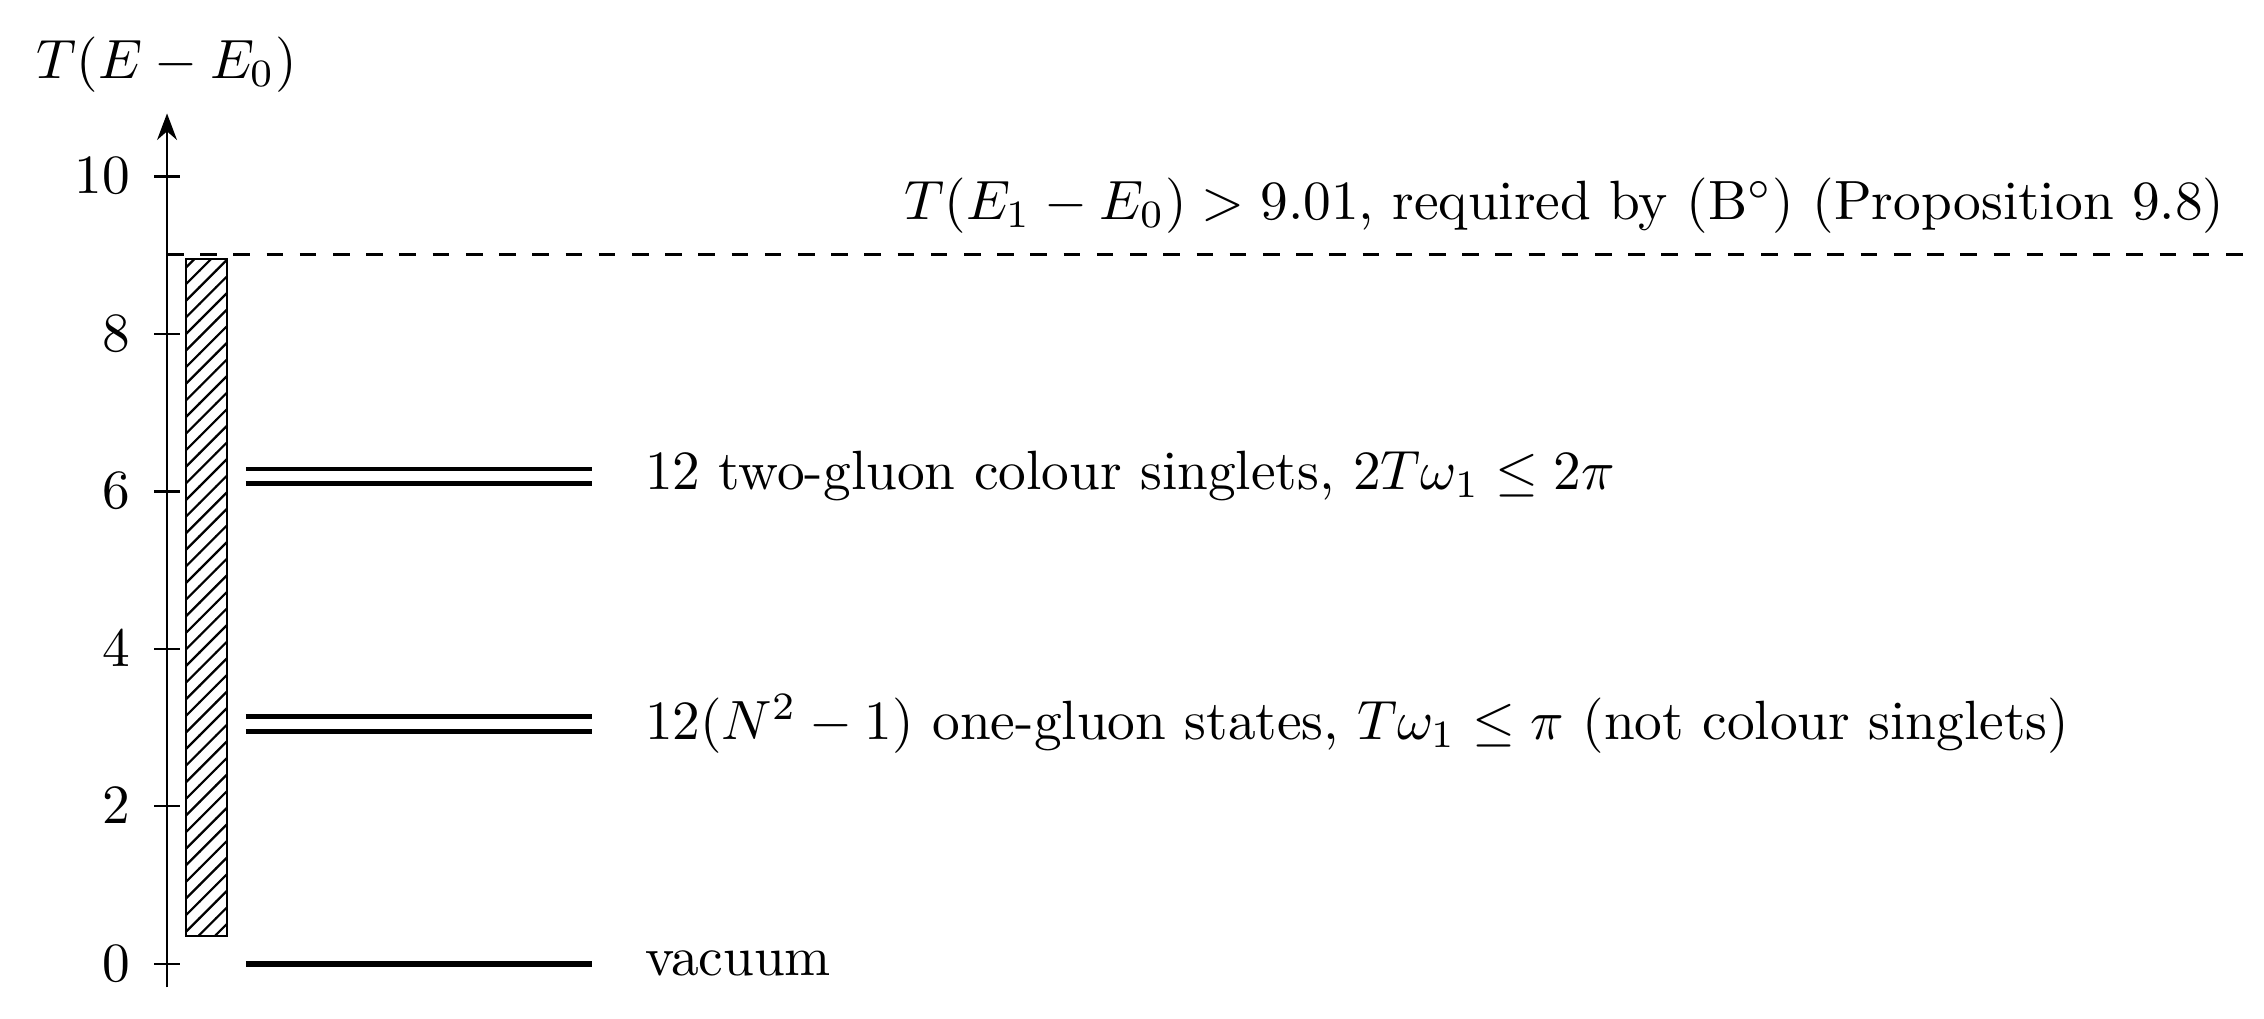
\includegraphics[width=407.4bp]{figures/fig13.png}
\caption{Energy levels of the harmonic reference $\Gharm$ on the cube $\cube T$, in units of $1/T$, against the threshold that \Bcirc{} imposes on every excited level (\cref{prop:no-stefan-boltzmann,thm:free-gluon}). The hatched strip marks the energies at which \Bcirc{} allows no level.}
\label{fig:levels}
\end{figure}

\Cref{fig:levels} shows the comparison. The next theorem makes it quantitative and shows that the violation does not depend on the scale.

\begin{theorem}[anatomy of the free-gluon violation]\label{thm:free-gluon}
Let $T\ge3$.
\begin{enumerate}[label=\textup{(\alph*)},leftmargin=*]
\item $X_\Gharm(T)\ge12(N^2-1)e^{-\pi}>0.518(N^2-1)$ and $\psi_\Gharm(T)\ge24(N^2-1)e^{-\pi}$; hence $X_\Gharm(T)\ge4248(N^2-1)/8192$ and $\psi_\Gharm(T)\ge4249(N^2-1)/4097$.
\item $X_\Gharm(T)\le34(N^2-1)$ for every $T\ge3$.
\item For every \PSTS{} satisfying \Bcirc{} at $T_0$, every eigenvalue $r_i=e^{-E_i}$, $i\ge1$, of $R$ on $\cube{T_0}$ satisfies $T_0E_i\ge-\log(e^{1/8192}-1)>9.0108$, and $\#\{i\ge1:T_0E_i\le x\}\le(e^{1/8192}-1)e^x$ for all $x$. The reference $\Gharm$ has $12(N^2-1)$ eigenvalues with $T_0E\le\pi$, each exceeding the largest value of $r^{T_0}$ allowed by \Bcirc{} by a factor greater than $e^{9.0108-\pi}>353$.
\item $X_\Gharm(T)\to2(N^2-1)\sum_{n\in\Z^3\setminus0}-\log(1-e^{-\pi\abs n})$ as $T\to\infty$.
\item For every \PSTS{} satisfying \Bcirc{} at $T_0$ and every $n\ge2T_0$, every eigenvalue $r=e^{-E}\ne r_0$ of $R$ on $(n,n,n)$ satisfies $nE\ge\log4096+\frac n{2T_0}\log\frac{63}{32}>8.317>2\pi$, whereas $\Gharm$ has $n\omega_1\le2\pi$ on every cube.
\item Let $k>1$ with $kT\in\Nat$ and $c_k=(2k/(k-1))^3$. Then $X_\Gharm((kT)^3,T)\ge12(N^2-1)\bigl(-\log(1-e^{-2\pi/k})\bigr)\ge972(N^2-1)c_k^{-2}$, while $(e^{c_kx}-1)^2\ge x$ for all $x\ge c_k^{-2}$. For $k=2$ the map $x\mapsto(e^{c_kx}-1)^2$ is the recursion of \cref{thm:ascent}.
\end{enumerate}
\end{theorem}

\begin{proof}
(a) For the six $n=\pm e_j$, $\sinh(\omega/2)=\sin(\pi/L)\le\pi/L$ with $L=2T$, and $\operatorname{arsinh}y\le y$, so $T\omega\le\pi$. Use $-\log(1-q)\ge q$ and $2\operatorname{artanh}q\ge2q$ on these $12(N^2-1)$ oscillators; all other terms are $\ge0$. Then $12e^{-\pi}>0.51856>4248/8192$ and $24e^{-\pi}>1.03713>4249/4097$.

(b) Take representatives $\abs{n_j}\le L/2$. By $\sin y\ge2y/\pi$ on $[0,\pi/2]$, $\sinh(\omega/2)\ge2\abs n/L$, and $2\abs n/L\le\sqrt3$. Since $\operatorname{arsinh}$ is concave, $\operatorname{arsinh}y\ge y\log(2+\sqrt3)/\sqrt3\ge0.76y$ on $[0,\sqrt3]$; hence $T\omega\ge1.52\abs n\ge b\abs n_1$ with $b=1.52/\sqrt3$. As $\abs n\ge1$, $q=e^{-T\omega}\le e^{-1.52}$ and $-\log(1-q)\le q/(1-e^{-1.52})$. The map from $n$ to its representative is injective into $\Z^3$, so
\[
X_\Gharm(T)\le\frac{2(N^2-1)}{1-e^{-1.52}}\Bigl[\Bigl(\frac{1+e^{-b}}{1-e^{-b}}\Bigr)^3-1\Bigr]\le33.88\,(N^2-1).
\]
(c) $r_i^{T_0}\le\Dexc{\cube{T_0}}{T_0}\le e^{1/8192}-1$, and $\Dexc{\cube{T_0}}{T_0}=\sum_{i\ge1}r_i^{T_0}\ge e^{-x}\#\{i\ge1:T_0E_i\le x\}$. The one-particle states $a^\dagger(f)\Omega$ with $f$ in the lowest shell, of dimension $12(N^2-1)$, have eigenvalue $e^{-\omega_1}$ with $T_0\omega_1\le\pi$ by (a). Finally $-\log(e^{1/8192}-1)>9.01085$ and $e^{9.0108-\pi}>353.9$.

(d) For fixed $n$, $L\sinh(\omega_n/2)\to\pi\abs n$, so $T\omega_n\to\pi\abs n$; dominated convergence applies with the summable majorant $e^{-b\abs n_1}/(1-e^{-1.52})$ of (b).

(e) By \cref{thm:ascent}(c), which applies to every \PSTS{} by \cref{lem:simplicity-not-needed}, $r^n\le\Dexc{n}{n}\le(32/63)^{n/(2T_0)}/4096$; and $12\log2>8.317>2\pi$. For $\Gharm$, $2\sinh(\omega_1/2)=2\sin(\pi/n)$ gives $n\omega_1\le2\pi$.

(f) The lowest shell on side $kT$ has $T\omega\le2\pi/k$ and $12(N^2-1)$ oscillators, which gives the first inequality. The second is $f(k):=-\log(1-e^{-2\pi/k})(2k/(k-1))^6\ge81$, and $972=12\cdot81$. For $k\le1.25$ the second factor is at least $10^6$ and the first at least $-\log(1-e^{-2\pi})>1.8\cdot10^{-3}$; for $k\ge20$ the second factor is at least $64$ and the first is increasing in $k$, with value $>1.31$ at $k=20$; on $[1.25,20]$ a grid of step $1/500$, with the two monotone factors evaluated at opposite ends of each cell, gives $f\ge81$ (\cref{app:certificates}). Finally $(e^{c_kx}-1)^2\ge(c_kx)^2\ge x$ for $x\ge c_k^{-2}$.
\end{proof}

By (b) the count is uniform in $T$, and by (d) the defect is a number of order $N^2-1$ independent of the scale: $8192\,X_\Gharm(T)\in[4248,\,34\cdot8192]\,(N^2-1)$ for all $T\ge3$. So no choice of $T_0$ helps, and $\Gharm$ fails the datum only through the gap. By (f), at the free-gluon value the majorant $(e^{c_kx}-1)^2$ does not contract for any aspect ratio $k$ of the base box; for $k=2$ it is the recursion of \cref{thm:ascent}.\footnote{Part (f) concerns the majorant $(e^{c_kx}-1)^2$ only; it is not a statement about every method of proof.}

\begin{theorem}[pair theorem]\label{thm:pair}
Let $\mathfrak h$ be a complex Hilbert space with an antiunitary involution $J$, and $\omega\ge0$ a self-adjoint operator on $\mathfrak h$ with discrete spectrum, $[\omega,J]=0$ and $\Tr\Gamma(e^{-T\omega})<\infty$. Let $H$ be a compact group acting on $\mathfrak h$ by unitaries $V_g$ that commute with $\omega$ and $J$, and $P_H$ the projection onto the $\Gamma(V)$-invariant vectors of the bosonic Fock space. For an eigenvalue $\omega_*$ of $\omega$ let $(e_i)$ be an orthonormal basis of $J$-fixed vectors of $E_*=\ker(\omega-\omega_*)$, and $\Phi_*=\sum_ia^\dagger(e_i)^2\Omega$. Then $\Phi_*\ne0$ is $H$-invariant, $\Gamma(e^{-\omega})\Phi_*=e^{-2\omega_*}\Phi_*$, and
\[
\Tr\bigl(P_H\Gamma(e^{-T\omega})\bigr)\ge1+\sum_{\omega_*\in\operatorname{spec}\omega}e^{-2T\omega_*}.
\]
For $\Gharm$ on $\cube{T_0}$, every group $H$ of real orthogonal maps of $\mathfrak h_\R$ commuting with $\omega$ satisfies the hypotheses, with $J$ the complex conjugation. This includes lattice translations, the cubic group and reflections acting on vector fields, charge conjugation $A\mapsto-A^{\mathsf T}$, and $\operatorname{Ad}(g)$, $g\in\SU(N)$. Each such $H$ gives
\[
\log\Tr\bigl(P_HR_\Gharm^{T_0}\bigr)\ge\log(1+e^{-2\pi})>\tfrac{15}{8192}.
\]
The centre of $\SU(N)$ acts trivially on adjoint fields, so the projection onto the centre-neutral sector leaves $X_\Gharm$ unchanged.
\end{theorem}

\begin{proof}
$J$ preserves $E_*$, and $E_*^\R=\{f\in E_*:Jf=f\}$ is a real form on which $\ip fg=\overline{\ip{Jf}{Jg}}=\overline{\ip fg}$ is real; so an orthonormal basis $(e_i)$ of $E_*^\R$ is an orthonormal basis of $E_*$, and $E_*$ is finite dimensional because $\Tr\Gamma(e^{-T\omega})<\infty$. Since $V_g$ preserves $E_*$ and commutes with $J$, $V_ge_i=\sum_jO_{ji}e_j$ with $O$ real orthogonal, and
\[
\Gamma(V_g)\Phi_*=\sum_{j,l}(OO^{\mathsf T})_{jl}\,a^\dagger(e_j)a^\dagger(e_l)\Omega=\Phi_*.
\]
The vectors $a^\dagger(e_i)^2\Omega$ are mutually orthogonal with norm $\sqrt2$, and $\Gamma(e^{-\omega})a^\dagger(e_i)^2\Omega=e^{-2\omega_*}a^\dagger(e_i)^2\Omega$. The vectors $\Omega$ and $\Phi_*/\norm{\Phi_*}$, one for each distinct $\omega_*$, are orthonormal eigenvectors in $\operatorname{Ran}P_H$, which commutes with $\Gamma(e^{-T\omega})$; the trace of $P_H\Gamma(e^{-T\omega})P_H\ge0$ is at least the sum of its diagonal entries on them. For $\Gharm$, $\omega$ is a real function of the real symmetric operator $-\Delta_\perp$, the listed maps are real orthogonal and commute with $-\Delta_\perp$, and the lowest shell has $T_0\omega_*\le\pi$ (\cref{thm:free-gluon}(a)). Finally $\log(1+y)\ge y-y^2/2>15/8192$ for $y=e^{-2\pi}$.
\end{proof}

The statement covers real symmetries only. By \cref{thm:pair} with the translations, the zero-momentum trace of $\Gharm$ still exceeds the bound $\xconstinl$ by a factor greater than $15$.

For $G=\SU(N)$, $\omega=e^{2\pi i/N}$, a four-torus $n=(n_1,\dots,n_4)$ and $\nu\in\Lambda^2\Z_N^4$, let $Z(n;\nu)$ be the Wilson integral with $Q_p$ replaced by $\omega^{\nu_{\mu\nu}}Q_p$ on one stack of $(\mu\nu)$-plaquettes in each plane. By \cref{lem:centre-operators} it does not depend on the stacks, and in the picture with time axis $\kappa$, writing $k\in\Z_N^3$ for the components $\nu_{j\kappa}$ and $m\in\Z_N^3$ for the three others, $Z(n;\nu)=\Tr\bigl(\TT^{(m)\,n_\kappa}z^k\bigr)$, where the twisted transfer matrix $\TT^{(m)}\ge0$ is Hilbert--Schmidt and commutes with $z^k$. Each $Z(n;\nu)$ is at least $1$, by Jensen's inequality, since each twisted plaquette variable is Haar distributed once one of its links is integrated.

\begin{theorem}[$\SU(N)/\Z_N$ exclusivity]\label{thm:exclusivity}
Let $G=\SU(N)$, $\beta\ge0$, all sides $\ge3$, and $\bar Z(n)=N^{-3}\sum_{\nu\in\Lambda^2\Z_N^4}Z(n;\nu)$, the sum over all $N^6$ twists.
\begin{enumerate}[label=\textup{(\roman*)},leftmargin=*]
\item $\bar Z$ is a \PSTS{} in the sense of \cref{lem:simplicity-not-needed}, with $\bar\TT_s=\bigoplus_{m\in\Z_N^3}P_0\TT_s^{(m)}P_0$ and $\bar\lambda_0=\lzero$; the block $m=0$ is the centre-neutral sector of $\SU(N)$.
\item $Z(n;\nu)\le Z(n;0)$ for all $\nu$; hence $N^3\le\bar Z\le N^3Z$.
\item On hypercubes $n^4$ let $D_n=\Dexc{n}{n}=D_n^0+D_n^{\ne}$ for $\SU(N)$, with $D_n^{\ne}=\sum_{e\ne0}\Zc_e$ the charged part, and $W_n=1-\Zc_0/\Zc$. Then
\[
\bar\Zc_n(n)\ge(q_N-4W_n)(1+D_n)=q_N(1+D_n^0)-(4-q_N)D_n^{\ne},\qquad q_N=\frac{4N^3-6N+3}{N^3}\ge\frac{23}8 .
\]
\item If $\bar Z$ satisfies \Bcirc{} at $T_0$, then $D_n^{\ne}>1.666$ and $W_n>0.468$ for every $n\ge2T_0$: the electric-flux sectors of $\SU(N)$ are far from suppressed. If $\SU(N)$ satisfies \Bcirc{} at $T_0'$, then $\bar\Zc_n(n)>2.874$ for every $n\ge2T_0'$, and $\bar Z$ satisfies \Bcirc{} at no $T_0$. The two data are mutually exclusive.
\end{enumerate}
\end{theorem}

\begin{proof}
(ii) For $A\ge0$ trace class and $U$ unitary commuting with $A$, $\abs{\Tr(AU)}\le\Tr A$. Apply this three times: picture $4$ deletes $\nu_{14},\nu_{24},\nu_{34}$; picture $1$ then deletes $\nu_{12},\nu_{13}$, the remaining spatial twist being $(\nu_{23},0,0)$ with $\TT^{(m')}_1\ge0$ (\cref{lem:centre-operators} in picture $1$); picture $2$ deletes $\nu_{23}$. Each $Z(n;\nu)$ is real and at least $1$, which gives the lower bound $N^{-3}N^6$.

(i) An axis permutation maps $\Lambda^2\Z_N^4$ bijectively to itself, and $Z(\pi n;\pi\nu)=Z(n;\nu)$ by hypercubic invariance; $\bar Z\ge1$. In picture $4$, with $P_0=N^{-3}\sum_kz^k$ commuting with $\TT^{(m)}$,
\[
N^{-3}\sum_\nu Z(s,M;\nu)=\sum_m\Tr\bigl(\TT^{(m)M}P_0\bigr)=\sum_m\Tr\bigl((P_0\TT^{(m)}P_0)^M\bigr),
\]
and $\bar\TT_s\ge0$ is Hilbert--Schmidt. Since $\Omegazero\in P_0\Kspace$, $\bar\lambda_0\ge\lzero$; by (ii), $\Tr\TT^{(m)M}=Z(s,M;(m,0))\le\Zpart sM$ for all $M$, so the top eigenvalue of every block is at most $\lzero$.

(iii) Let $S_\kappa=\{\nu:\nu_{\mu\nu}=0$ unless $\kappa\in\{\mu,\nu\}\}$, so $\abs{S_\kappa}=N^3$. In picture $\kappa$ the twists in $S_\kappa$ are purely temporal, so $\sum_{\nu\in S_\kappa}Z(n;\nu)=\sum_k\Tr(\TT_\kappa^nz^k)=N^3\Tr(P_0\TT_\kappa^n)=N^3(1-W_n)Z(n)$; on the hypercube the four pictures are related by symmetry and share $W_n$. The pairwise intersections $S_\kappa\cap S_\lambda$ consist of the $N$ twists in the plane $\kappa\lambda$ and have sum at most $NZ$ by (ii); the four triple intersections and the quadruple intersection are $\{0\}$, with sum $Z$. Since all terms are nonnegative, inclusion and exclusion give
\[
\bar Z(n)\ge N^{-3}\bigl[4N^3(1-W_n)-6N+4-1\bigr]Z(n)=(q_N-4W_n)Z(n).
\]
Divide by $\lzero^n=\bar\lambda_0^n$ and use $W_n(1+D_n)=\Zc-\Zc_0=D_n^{\ne}$. Finally $q_N=4-6/N^2+3/N^3$ increases in $N$ and $q_2=23/8$.

(iv) By (i), \cref{lem:simplicity-not-needed} and \cref{thm:ascent}(c), \Bcirc{} for $\bar Z$ at $T_0$ gives $\bar\Zc_n(n)\le\frac{4097}{4096}$ for $n\ge2T_0$. Then $q_N-(4-q_N)D_n^{\ne}\le\bar\Zc_n(n)\le\frac{4097}{4096}$ gives $D_n^{\ne}\ge(q_N-\frac{4097}{4096})/(4-q_N)$, which increases in $N$ and is $>1.666$ at $N=2$. Likewise $q_N-4W_n\le\max\{0,(q_N-4W_n)(1+D_n)\}\le\frac{4097}{4096}$ gives $W_n\ge(q_N-\frac{4097}{4096})/4>0.468$. Conversely, \Bcirc{} for $\SU(N)$ at $T_0'$ gives $D_n\le1/4096$ for $n\ge2T_0'$ by \cref{thm:ascent}(c), so $\bar\Zc_n(n)\ge q_N-(4-q_N)/4096\ge\frac{23}8-\frac98\cdot\frac1{4096}>2.874>\frac{4097}{4096}$. For $n\ge\max\{2T_0,2T_0'\}$ this contradicts \Bcirc{} for $\bar Z$ at any $T_0$.
\end{proof}

\subsection{Finite-volume gaps and triviality}

For $d\in\{2,3,4\}$, $T_0\ge3$ and a spatial torus $s=(s_1,\dots,s_{d-1})$ in the window $2T_0\le s_j<48T_0$, put $\theta_s=\Vol s/(161(48T_0)^{d-1})$, $\Vol s=\prod_js_j$. The datum $(\mathrm D_d)$ at $s$ is $\psiT{s}{T_0}\le\theta_s$; for $d=4$ it is \cref{ms:eq:rational-condition}. Let $\varrho(p)=(1-\sqrt{2p-1})/(1+\sqrt{2p-1})$ for $p\in(\frac12,1]$, the sharp function of \cref{ms:thm:sharp}. The Gaussian reference in dimension $d$ carries $(d-2)(N^2-1)$ oscillators of frequency $\omega_p$, $4\sinh^2(\omega_p/2)=\sum_j4\sin^2(p_j/2)$, for each nonzero $p\in\prod_j\frac{2\pi}{s_j}\Z_{s_j}$; for $d=4$ it is $\Gharm$. Its purity defect is $\psi_{\mathrm{ref}}=(d-2)(N^2-1)\sum_{p\ne0}2\operatorname{artanh}e^{-T_0\omega_p}$.

\begin{proposition}[the datum forces a finite-volume gap in every dimension]\label{prop:finite-volume-gap}
\leavevmode
\begin{enumerate}[label=\textup{(\alph*)},leftmargin=*]
\item If $(\mathrm D_d)$ holds at $s$ for the $d$-dimensional Wilson theory of a compact group, then $\delta(s)=-\log(\lambda_1/\lzero)$ satisfies $\delta(s)\ge T_0^{-1}\log\bigl(1/\varrho(e^{-\theta_s})\bigr)$. On the smallest box $s=(2T_0)^{d-1}$, with $\ell=2T_0$, this reads $\delta\ell\ge30.6$ for $d=4$, $\delta\ell\ge24.2$ for $d=3$ and $\delta\ell\ge17.9$ for $d=2$.
\item For every $s$ in the window, $\psi_{\mathrm{ref}}\ge X_d(N^2-1)\theta_s$ with $X_4=125000$ and $X_3=4300$; for $d=2$, $\psi_{\mathrm{ref}}=0$.
\end{enumerate}
\end{proposition}

\begin{proof}
(a) The datum gives the purity $Z(s,2T_0)/Z(s,T_0)^2=e^{-\psiT{s}{T_0}}\ge e^{-\theta_s}>\frac12$, and \cref{ms:thm:sharp} gives $(\lambda_1/\lzero)^{T_0}\le\varrho(e^{-\theta_s})$, since $\varrho$ is decreasing. On the smallest box $\theta=1/(161\cdot24^{d-1})$, which is $1/2225664$, $1/92736$ and $1/3864$ for $d=4,3,2$. For $0\le\theta\le\sqrt2-1$, $\sqrt{2e^{-\theta}-1}\ge\sqrt{1-2\theta}\ge1-\theta-\theta^2$, hence $\varrho\le(\theta+\theta^2)/(2-\theta-\theta^2)$, and $1/\varrho>e^{15.3},e^{12.1},e^{8.95}$ respectively; multiply by $2$.

(b) For $d=2$ there are no oscillators. Otherwise use $2\operatorname{artanh}q\ge2q$ and $\omega_p\le\abs p$, which follows from $\operatorname{arsinh}y\le y$ and $\abs{\sin y}\le\abs y$. Put $m_j=\lfloor s_j/(2T_0)\rfloor\ge1$ and keep only the modes $p_j=2\pi n_j/s_j$ with $\abs{n_j}\le m_j$, $n\ne0$; they are distinct, since $m_j\le s_j/6<s_j/2$, and satisfy $T_0\abs p\le\pi\sqrt{d-1}$. With $x=s_j/(2T_0)\ge1$ one has $2\lfloor x\rfloor+1\ge\frac32x$, and the product of the $2m_j+1$ is at least $3^{d-1}$, so the number of kept modes is at least $(1-3^{1-d})(\frac34)^{d-1}\Vol s/T_0^{d-1}$. For $d=4$ this gives $\psi_{\mathrm{ref}}\ge\frac{13}8(N^2-1)e^{-\pi\sqrt3}\Vol s/T_0^3$, and $\frac{13}8\cdot17805312\,e^{-\pi\sqrt3}\ge125381$. For $d=3$ it gives $\psi_{\mathrm{ref}}\ge(N^2-1)e^{-\pi\sqrt2}\Vol s/T_0^2$, and $370944\,e^{-\pi\sqrt2}\ge4363$.
\end{proof}

The Gaussian reference has $\delta\ell\le2\pi$, since its lowest mode has $2\sinh(\omega/2)=2\sin(\pi/\ell)$. In two dimensions there are no transverse modes, (b) is void, and the datum holds (\cref{thm:two-dim}).

A \emph{Hamiltonian continuum limit} is given by the following data: for $k\in\Nat$ a Hilbert space $\Hilb_k$, a unit vector $\Omega_k$ and a self-adjoint $H_k\ge0$ with $H_k\Omega_k=0$ and $\sigma(H_k)\cap(0,\delta_k)=\emptyset$, $\delta_k\in[0,\infty]$; spacings $a_k\to0$; a complex vector space $\mathcal T$ with linear maps $\psi_k\colon\mathcal T\to\Hilb_k$; a set $D\subset[0,\infty)$, dense in $[0,\infty)$, containing $0$ and a sequence $\tau_n\downarrow0$; and a limit $(\Hilb,\Omega,H,\psi)$, with $H\ge0$ self-adjoint, $H\Omega=0$ and $\psi\colon\mathcal T\to\Hilb$ linear with dense range, such that for all $f,f'\in\mathcal T$ and $\tau\in D$
\[
\ip{\psi(f)}{e^{-\tau H}\psi(f')}=\lim_k\ip{\psi_k(f)}{e^{-\tau H_k/a_k}\psi_k(f')},\qquad\ip\Omega{\psi(f)}=\lim_k\ip{\Omega_k}{\psi_k(f)}.
\]
This is \cite[Lemma~A32]{bhattacharjee2026first} (restated in \cref{app:first-paper}) with the transfer matrix $T_k^{\tau/a_k}$ replaced by $e^{-\tau H_k/a_k}$; the proof is the same, and we give it.

\begin{proposition}[gaps in lattice units are triviality statements]\label{prop:lattice-unit-triviality}
\leavevmode
\begin{enumerate}[label=\textup{(\alph*)},leftmargin=*]
\item Let $\bar E=\limsup_k\delta_k/a_k\in[0,\infty]$. Then $\ip\varphi{e^{-\tau H}\varphi}\le e^{-\bar E\tau}\norm\varphi^2$ for $\varphi\in\Omega^\perp$ and $\tau\ge0$, so $\sigma(H|_{\Omega^\perp})\subset[\bar E,\infty)$, and $\Omega^\perp=\{0\}$ if $\bar E=\infty$. In particular, if $\liminf_k\delta_k>0$, then $\Hilb=\C\Omega$; and a nontrivial limit requires $\delta_k=O(a_k)$, so $\delta_k\to0$.
\item If $\delta_k\ge c\,g_k^{2m}$ for some $c>0$ and $m\ge0$, and $g_k^{-2}\le C\log(1/a_k)$ for large $k$, then $\delta_k/a_k\to\infty$ and the limit is trivial.
\end{enumerate}
\end{proposition}

\begin{proof}
(a) Fix $f\in\mathcal T$ and put $\varphi_k=\psi_k(f)-\ip{\Omega_k}{\psi_k(f)}\Omega_k\perp\Omega_k$ and $\varphi=\psi(f)-\ip\Omega{\psi(f)}\Omega\in\Omega^\perp$. Since $e^{-\tau H_k/a_k}$ is self-adjoint, fixes $\Omega_k$ and preserves $\Omega_k^\perp$, the spectral theorem and $\sigma(H_k)\cap(0,\delta_k)=\emptyset$ give $\ip{\varphi_k}{e^{-\tau H_k/a_k}\varphi_k}\le e^{-\tau\delta_k/a_k}\norm{\varphi_k}^2$. The left side equals $\ip{\psi_k(f)}{e^{-\tau H_k/a_k}\psi_k(f)}-\abs{\ip{\Omega_k}{\psi_k(f)}}^2$, which converges for $\tau\in D$ to $\ip{\psi(f)}{e^{-\tau H}\psi(f)}-\abs{\ip\Omega{\psi(f)}}^2=\ip\varphi{e^{-\tau H}\varphi}$; the case $\tau=0$ gives $\norm{\varphi_k}^2\to\norm\varphi^2$. Along a subsequence with $\delta_k/a_k\to\bar E$ the right side converges to $e^{-\bar E\tau}\norm\varphi^2$ (to $0$ if $\bar E=\infty$ and $\tau>0$). So the bound holds for $\tau\in D$ on the projection of $\psi(\mathcal T)$ to $\Omega^\perp$, which is dense in $\Omega^\perp$; by continuity in $\varphi$ it holds on $\Omega^\perp$, and by strong continuity of the semigroup and density of $D$ for all $\tau\ge0$. If $\bar E=\infty$, then $\ip\varphi{e^{-\tau_nH}\varphi}=0$ along $\tau_n\downarrow0$, and strong continuity at $0$ gives $\varphi=0$. If $\bar E<\infty$ and the spectral measure $\mu_\varphi$ of some $\varphi\in\Omega^\perp$ had $\mu_\varphi([0,\bar E-\eta])=c>0$, then $\ip\varphi{e^{-\tau H}\varphi}\ge ce^{-(\bar E-\eta)\tau}>e^{-\bar E\tau}\norm\varphi^2$ for large $\tau$; so $\sigma(H|_{\Omega^\perp})\subset[\bar E,\infty)$. If $\liminf\delta_k>0$, then $\bar E=\infty$ because $a_k\to0$; if $\Omega^\perp\ne\{0\}$, then $\bar E<\infty$, so $\delta_k\le(\bar E+1)a_k$ for large $k$.

(b) $\delta_k/a_k\ge c\,a_k^{-1}(C\log(1/a_k))^{-m}\to\infty$; apply (a).
\end{proof}

Every asymptotic-freedom tuning $g^{-2}=2b_0\log(1/(a\Lambda))+O(\log\log(1/a))$ satisfies the hypothesis of (b). Along such tunings a nontrivial limit forces the lattice-unit gap to be $o(g_k^{2m})$ for every $m$: smaller than every power of the coupling. A lattice gap is not necessary for a continuum gap, but the upper bound $\delta_k=O(a_k)$ is necessary for nontriviality.

The last result concerns limits that are trivial for a different reason. A \emph{cluster} $F$ is a fixed-stencil gauge-invariant insertion with a test function on pairwise distinct points, as in \cite[Definition~3]{bhattacharjee2026first}, and $S(F)=\lim_kS_k(F)$ is the limit of its lattice smears, assumed to exist for all clusters and to be continuous under translations of the test function; both are part of \hypW. With $\vartheta_0$ the time reflection, $S(\vartheta_0\bar F)=\overline{S(F)}$, and the time-zero Osterwalder--Schrader form $\ip FG_0=S(\vartheta_0\bar F\cdot G)$ for clusters supported in $\{x_0>0\}$ defines $\Hilb$ by completion. For $j\in\{1,2,3\}$, $\vartheta_j$ is the reflection $x_j\mapsto-x_j$ and $\ip FG_j=S(\vartheta_j\bar F\cdot G)$ for clusters supported in $\{x_j>0\}$.

\begin{theorem}[a spatially finite correlation length and one rotation give a trivial limit]\label{thm:rotation-triviality}
\leavevmode
\begin{enumerate}[label=\textup{(\alph*)},leftmargin=*]
\item Let $j\in\{1,2,3\}$ and $R\in\mathrm O(4)$ with $Re_0=\pm e_j$. Suppose $R$ acts on clusters multiplicatively, commuting with complex conjugation and with $R\vartheta_0=\vartheta_jR$, and that $S(RF)=S(F)$ for all clusters. Suppose further that either
\begin{enumerate}[label=\textup{(a\arabic*)},leftmargin=*]
\item $S(FG)=S(F)S(G)$ whenever the supports of $F$ and $G$ are separated by a hyperplane $\{x_j=\mathrm{const}\}$; or
\item $Re_0=e_j$, the lattice states are reflection positive in direction $j$, and their gaps $m^{(j)}_k$ and spacings $a^{(j)}_k$ in direction $j$ satisfy $\limsup_km^{(j)}_k/a^{(j)}_k=\infty$.
\end{enumerate}
Then $\ip FG_0=\overline{S(F)}S(G)$ for all clusters $F,G$ supported in $\{x_0>0\}$, and $\Hilb=\C\Omega$.
\item Let $f\colon[0,\infty)\to\R$ be continuous with $\abs f\le f(0)$, $f(\tau)=f(0)-o(\tau)$ as $\tau\downarrow0$, and $\sum_{a,b}d_ad_bf(\tau_a+\tau_b)\ge0$ for all finite families $\tau_a>0$, $d_a\in\R$. Then $f\equiv f(0)$.
\item Let $X(\tau)$, $\tau\in\R$, be a real second-order process with covariance $\mathbb E[X(\tau)X(\tau')]=f(\abs{\tau-\tau'})$, $f$ continuous and $\tau\mapsto f(\abs\tau)$ differentiable at $0$. If the covariance is reflection positive, $\sum_{a,b}d_ad_b\,\mathbb E[X(-\tau_a)X(\tau_b)]\ge0$ for all $\tau_a>0$ and $d_a\in\R$, then $X(\tau)=X(0)$ with probability one, for every $\tau$.
\end{enumerate}
\end{theorem}

\begin{proof}
(a) Let $F,G$ be supported in $\{x_0>0\}$. Under (a1): $R$ maps $\{x_0<0\}$ and $\{x_0>0\}$ to the two sides of $\{x_j=0\}$, so $R(\vartheta_0\bar F)$ and $RG$ are separated by that hyperplane, and
\[
\ip FG_0=S\bigl(R(\vartheta_0\bar F)\cdot RG\bigr)=S\bigl(R\vartheta_0\bar F\bigr)\,S(RG)=S(\vartheta_0\bar F)\,S(G)=\overline{S(F)}\,S(G).
\]
Under (a2): $RF,RG$ are supported in $\{x_j>0\}$ and $R(\vartheta_0\bar F)=\vartheta_j\overline{RF}$. \Cref{prop:lattice-unit-triviality}(a), or \cite[Lemma~A32]{bhattacharjee2026first}, applied in direction $j$ shows that the direction-$j$ reconstruction is one-dimensional, so $\ip{RF}{RG}_j=\overline{S(RF)}S(RG)$, the vacuum class pairing with the class of a cluster $H$ to $S(H)$. Hence $\ip FG_0=S(\vartheta_j\overline{RF}\cdot RG)=\overline{S(RF)}S(RG)=\overline{S(F)}S(G)$. In both cases the form $\ip\cdot\cdot_0$ has rank at most one, so $\Hilb=\C\Omega$.

(b) One point gives $f\ge0$ on $(0,\infty)$, and two points give $f(\frac{u+v}2)^2\le f(u)f(v)$ for $u,v>0$. If $f(u)=0$ for some $u>0$, then $f(s+\frac u2)^2\le f(2s)f(u)=0$ for all $s>0$, so $f=0$ on $(u/2,\infty)$; by iteration and continuity $f\equiv0$. Otherwise $\log f$ is continuous and midpoint convex on $(0,\infty)$, hence convex, so $f$ is convex on $[0,\infty)$. For $0<h<\tau$, $(f(h)-f(0))/h\le(f(\tau)-f(0))/\tau$, and letting $h\downarrow0$ gives $f(\tau)\ge f(0)$; with $f\le f(0)$, equality holds.

(c) $\abs f\le f(0)$ by Cauchy--Schwarz, and $f(\tau)=f(0)+o(\tau)$ because an even function differentiable at $0$ has derivative $0$ there. Reflection positivity is the hypothesis of (b) with $\mathbb E[X(-\tau_a)X(\tau_b)]=f(\tau_a+\tau_b)$, so $f\equiv f(0)$ and $\mathbb E(X(\tau)-X(0))^2=2f(0)-2f(\tau)=0$.
\end{proof}

Part (a) covers anisotropic tunings with a temporal gap that is finite in physical units and a spatial correlation length bounded in lattice units, which \cref{prop:lattice-unit-triviality} alone does not reach. Bounded tokens give c-number limit fields under \hypW{} (\cref{thm:bounded-tokens}); by (c), a reflection-positive field that is regular at coinciding times does not depend on time.\footnote{Suppose a gradient-flowed observable at fixed flow time, such as the flowed action density, had a continuum limit as a translation- and reflection-invariant second-order random field that is mean-square differentiable in $x_0$. By (c) its correlation functions would be reflection positive only if the field did not depend on $x_0$. The differentiability hypothesis is heuristic (it is what the flow is designed to provide), and this reading is not part of any theorem.}

\subsection{Blocked fields at the scale of the box}\label{sec:box-disorder}

Throughout this subsection $T_0=qb\ge3$ with integers $q,b\ge1$, $t=\cube{T_0}$, and $\mu^0_t$, $R$, $r_1=r_1(t)$ and $\Omegazero$ are as in the conventions of this section. Functions of a slab, slab operators $\hat F$, $\Psi_F=\lzero^{-w}\hat F\Omegazero$, the time reflection $\vartheta$ and the time translations $\tau_s$ are those of \cref{lem:gap-decay}, on the spatial torus $t$; \cref{lem:gap-decay}(a) holds on every spatial torus by the proof of \cref{lem:fp-slice}(a). The \emph{coarse torus} is $\bar t=(\Z/2q\Z)^3$, with sites $\bar\Lambda$ and links $\bar E$. For $c$ in the centre of $G$ and $j\le3$, $\hat\zeta^c_j$ is the fine centre flip of \cref{lem:fp-slice}(b) and $\bar\zeta^c_j$ multiplies the coarse links $(y,j)$ with $y_j=0$ by $c$.

\begin{definition}[blockings]\label{def:blocking}
Let $0\le w\le b$. A \emph{blocking} of block size $b$ and depth $w$ is a measurable map $U\mapsto\bar Q^{(0)}(U)\in G^{\bar E}$ which is a function of the slab $[0,w]$ and satisfies
\begin{enumerate}[label=\textup{(B\arabic*)},leftmargin=*]
\item \emph{centre covariance:} $\bar Q^{(0)}\circ\hat\zeta^c_j=\bar\zeta^c_j\,\bar Q^{(0)}$ almost everywhere, for every $j\le3$ and every $c$ in the centre of $G$.
\end{enumerate}
The \emph{coarse slices} are $\bar Q^{(n)}=\tau_{nb}\bar Q^{(0)}$, $n\in\Z$, functions of the slabs $[nb,nb+w]$. Let $\bar P_j(n)$ be the ordered product of the $2q$ links of $\bar Q^{(n)}$ from the origin once around direction $j$, and for a word $W$ in $P_1^{\pm1},P_2^{\pm1},P_3^{\pm1}$ let $F_W(n)=\Tr W(\bar P_1(n),\bar P_2(n),\bar P_3(n))=\tau_{nb}F_W(0)$. The blocking is a \emph{slice blocking} if $w=0$, and it is \emph{reflection covariant} if
\begin{enumerate}[label=\textup{(B\arabic*)},leftmargin=*,resume]
\item $\vartheta F_W(0)=\tau_{-w}F_W(0)$ for every word $W$, that is, each $F_W(0)$ is invariant under the reflection of the slab $[0,w]$ in its midpoint.
\end{enumerate}
A \emph{temporal completion} is an arbitrary measurable choice of $\bar U^{(n)}(U)\in G^{\bar\Lambda}$, $n\in\{-1,0\}$; no locality, covariance or other condition is imposed. For $e=(y,j)\in\bar E$ and $n\in\{-1,0\}$ the \emph{coarse temporal plaquette} is $\bar Q_{e,n}=\bar Q^{(n)}_{(y,j)}\bar U^{(n)}_{y+e_j}\bigl(\bar Q^{(n+1)}_{(y,j)}\bigr)^*\bigl(\bar U^{(n)}_y\bigr)^*$, and
\[
\delta(\bar Q,\bar U)=\max_{n\in\{-1,0\}}\ \sup_{e\in\bar E}\ \mu^0_t\bigl(\tfrac12\norm{\bar Q_{e,n}-1}_F^2\bigr),\qquad \delta_*(\bar Q)=\inf_{\bar U}\delta(\bar Q,\bar U).
\]
\end{definition}

Every slice blocking is reflection covariant, since $\vartheta$ fixes the spatial links at time $0$. Gauge covariance of $\bar Q^{(0)}$ is natural but is not used below. The quantity $\delta_*$ depends only on the coarse slices: it measures how far the coarse spatial fields at times $-b$, $0$ and $b$ are from each other modulo coarse gauge transformations.

\begin{theorem}[disorder at the scale of the box]\label{thm:box-disorder}
Let $G=\SU(2)$, $\beta\ge0$, let $\bar Q$ be a blocking of block size $b$ on $t=\cube{T_0}$, $T_0=qb\ge3$, let $\bar U$ be a temporal completion and $\delta=\delta(\bar Q,\bar U)$.
\begin{enumerate}[label=\textup{(\alph*)},leftmargin=*]
\item If $\bar Q$ is a slice blocking, then $1-r_1^b\le56\,q^2\delta$.
\item If $\bar Q$ is reflection covariant, then $r_1^b\ge1-224\,q^2\delta$.
\item Consequently $r_1^{T_0}\ge(1-56q^2\delta)_+^q\ge1-56q^3\delta$ in case \textup{(a)}, and $r_1^{T_0}\ge(1-224q^2\delta)_+^q\ge1-224q^3\delta\ge1-56q^2(q+1)^2\delta$ in case \textup{(b)}.
\item If \Bcirc{} holds at $T_0$, in particular if \Mcirc{} does, then with $x_q=9.0107/q$
\[
56\,q^2\,\delta_*(\bar Q)\ge1-e^{-x_q}\ge0.632\min\{1,x_q\}\quad\text{in case (a)},\qquad 224\,q^2\,\delta_*(\bar Q)\ge1-e^{-x_q}\quad\text{in case (b)}.
\]
For $q=1$ this reads $\delta_*\ge1/56.01$, respectively $\delta_*\ge1/224.03$.
\item For $G=\SU(N_c)$, with the words $\mathcal W$ and the constants $\gamma_{N_c}$ and $K_{N_c}$ of \cref{thm:SUN-gap}\textup{(b)}, parts \textup{(a)--(d)} hold with $56$ replaced by $4K_{N_c}$ and $224$ by $16K_{N_c}$.
\end{enumerate}
\end{theorem}

\begin{proof}
\emph{Charged words.} Let $W$ be one of the eleven words of \cref{lem:lemma-W}, with weight $w_W$ and $m_W$ steps on $\bar t$; thus $m_W=2q$, $4q$ or $6q$, and $\sum_Ww_Wm_W^2=28q^2$ by the computation of the bracket in \cref{thm:fixed-torus-gap} with $\ell=2q$. The function $F_W(n)$ is real, bounded by $2$, and a function of the slab $[nb,nb+w]$. The loop of $\bar P_j(n)$ contains exactly one coarse link $(y,j)$ with $y_j=0$, and the loops of $\bar P_i(n)$, $i\ne j$, contain no link in direction $j$; since $\hat\zeta^{-1}_j$ commutes with $\tau_{nb}$, \textup{(B1)} gives $\bar P_j(n)\circ\hat\zeta^{-1}_j=-\bar P_j(n)$ and $\bar P_i(n)\circ\hat\zeta^{-1}_j=\bar P_i(n)$. Every letter of $W$ occurs once, so $F_W(n)\circ\hat\zeta^{-1}_j=-F_W(n)$ for some $j$, and $\mu^0_t(F_W(n))=0$ by \cref{lem:fp-slice}(b). By \cref{lem:lemma-W}, $\sum_Ww_WF_W(n)^2=\Phi(\bar P(n))\ge1$ pointwise.

\emph{Strip interpolation.} Let $n<n'$ in $\{-1,0,1\}$. Repeating the interpolation in the proof of \cref{thm:fixed-torus-gap} with the coarse links of the slices $p$ and $p+1$ in place of $e_k$, $e'_k$ and with $\bar U^{(p)}$ in place of the temporal links, for $p=n,\dots,n'-1$, gives pointwise
\[
\abs{F_W(n)-F_W(n')}\le\sqrt2\sum_{p=n}^{n'-1}\sum_{k=1}^{m_W}\norm{Q_{k,p}-1}_F ,
\]
where $Q_{k,p}$ is $\bar Q_{e,p}$ for the $k$-th link $e$ of the loop, or a conjugate of $\bar Q_{e,p}^*$ if the loop traverses $e$ backwards; in both cases $\norm{Q_{k,p}-1}_F=\norm{\bar Q_{e,p}-1}_F$. The algebraic identity used there holds for arbitrary group elements on the links of the strip. By Cauchy--Schwarz and $\norm{Q-1}_F^2=2A_Q$,
\begin{equation}\label{eq:box-strip}
\tfrac12\,\mu^0_t\bigl((F_W(n)-F_W(n'))^2\bigr)\le2\,(n'-n)^2m_W^2\,\delta .
\end{equation}

(a) Here $F_W(0)$ is a bounded slice function and $F_W(1)=\tau_bF_W(0)$. By \cref{eq:fp-slice} and $\tau_b$-invariance, $\ip{F_W(0)\Omegazero}{(1-R^b)F_W(0)\Omegazero}=\frac12\mu^0_t((F_W(0)-F_W(1))^2)\le2m_W^2\delta$. Since $F_W(0)\Omegazero\perp\Omegazero$ and $0\le R^b\le r_1^b$ on $\Omegazero^\perp$ (\cref{lem:transfer-matrix}(i), \cref{lem:fp-slice}(d)), $(1-r_1^b)\mu^0_t(F_W(0)^2)\le2m_W^2\delta$. Multiplying by $w_W$ and summing, $(1-r_1^b)\,\mu^0_t(\Phi(\bar P(0)))\le56q^2\delta$, and $\mu^0_t(\Phi)\ge1$.

(b) Put $a=b-w\ge0$ and $\Psi_W=\Psi_{F_W(0)}$, for the slab $[0,w]$. By \textup{(B2)}, $F_W(-1)=\tau_{-b}F_W(0)=\tau_{-a}\vartheta F_W(0)$. Translation invariance of $\mu^0_t$ and \cref{lem:gap-decay}(a) give, for integers $s\ge0$,
\[
C_W(s):=\mu^0_t\bigl(F_W(-1)\,F_W(s)\bigr)=\mu^0_t\bigl(\vartheta F_W(0)\,\tau_{sb+a}F_W(0)\bigr)=\ip{\Psi_W}{R^{sb+a}\Psi_W},
\]
and $\ip{\Omegazero}{\Psi_W}=\mu^0_t(F_W(0))=0$. The subspace $\Omegazero^\perp$ is invariant and $0\le R\le r_1$ there, so $\lambda^{b+a}\le r_1^b\lambda^a$ on the spectrum gives $0\le C_W(1)\le r_1^bC_W(0)$, with $C_W(0)\ge0$. By Cauchy--Schwarz and $\tau_b$-invariance, $C_W(0)\le\mu^0_t(F_W(0)^2)$; and since $\mu^0_t(F_W(\pm1)^2)=\mu^0_t(F_W(0)^2)$, \eqref{eq:box-strip} with $n'-n=2$ gives $C_W(1)=\mu^0_t(F_W(0)^2)-\frac12\mu^0_t((F_W(-1)-F_W(1))^2)\ge\mu^0_t(F_W(0)^2)-8m_W^2\delta$. With $S=\mu^0_t(\Phi(\bar P(0)))\ge1$, the weighted sums give
\[
r_1^b\,S\ \ge\ r_1^b\sum_Ww_WC_W(0)\ \ge\ \sum_Ww_WC_W(1)\ \ge\ S-224q^2\delta ,
\]
and dividing by $S$ gives (b).

(c) $r_1^{T_0}=(r_1^b)^q$, and $(1-y)_+^q\ge1-qy$ for $y\ge0$; finally $4q\le(q+1)^2$.

(d) By \cref{prop:spectral-conditions}(iii), \Bcirc{} at $T_0$ gives $r_1^{T_0}\le e^{-9.0107}$, so $r_1^b\le e^{-x_q}$, and (a), (b) give the bounds for every temporal completion, hence for $\delta_*$. The bound $1-e^{-x}\ge(1-e^{-1})\min\{1,x\}$ is concavity, as in \cref{cor:base-scale}(a). For $q=1$, $1-e^{-9.0107}>0.99987$, $56/0.99987<56.01$ and $224/0.99987<224.03$.

(e) Use $F=\operatorname{Re}\Tr W(\bar P(n))$ and $F=\operatorname{Im}\Tr W(\bar P(n))$ for $W\in\mathcal W$. With $c=e^{2\pi i/N_c}$, \textup{(B1)} multiplies $\Tr W(\bar P(n))$ by $c^{n_j(W)}$ under $\hat\zeta^c_j$, and $n_j(W)\not\equiv0\pmod{N_c}$ for some $j$, so both parts have mean $0$ by \cref{lem:fp-slice}(b); pointwise $\sum_{W\in\mathcal W}\abs{\Tr W}^2\ge\gamma_{N_c}$. By $\abs{\Tr Z}\le\sqrt{N_c}\norm Z_F$ the two strip bounds sum to $\frac12\mu^0_t\abs{\Tr W(\bar P(n))-\Tr W(\bar P(n'))}^2\le N_c(n'-n)^2m_W^2\delta$, and $m_W\le2q\abs W$. Steps (a) and (b) then give $(1-r_1^b)\gamma_{N_c}\le4q^2N_c\sum_W\abs W^2\delta$ and $r_1^b\ge1-16q^2N_c\sum_W\abs W^2\delta/\gamma_{N_c}$, which are the claims with $K_{N_c}=(N_c/\gamma_{N_c})\sum_W\abs W^2$; (c) and (d) follow as before.
\end{proof}

\emph{Examples.} (i) With $b=1$, $\bar Q^{(0)}$ the fine slice at time $0$ and the fine temporal links as completion, $\delta\le\varepsilon(c)$ for $c\ge\frac1{32}$ (proof of \cref{thm:fixed-torus-gap}), and \cref{thm:box-disorder}(d) is the footnote to \cref{cor:base-scale}(c). (ii) Straight-line decimation, $\bar Q^{(0)}_{(y,j)}$ the product of the $b$ fine links of time $0$ from $by$ in direction $j$, is a slice blocking; the coarse loops are the fine loops. (iii) Spatial smearing followed by decimation, for instance the three-dimensional Wilson flow of the time-$0$ slice for a fixed flow time, is a slice blocking: the flow is the gradient flow of $S_s$ for the bi-invariant metric, and $\zeta^c_j$ is an isometry preserving $S_s$ (proof of \cref{lem:transfer-matrix}(iv)), so the flow commutes with $\zeta^c_j$. (iv) Block averaging in the time slab $[0,b-1]$ has depth $w=b-1$, and \textup{(B2)} asks that it be equivariant under the reflection of that slab in its midpoint. Smearing by the four-dimensional heat kernel or Wilson flow is not a blocking: the smeared slice depends on all times, so the slab condition fails.

The theorem is a necessary condition on \Mcirc{}, not evidence for or against it. It has content only for blockings whose coarse slices can be shown to be close to each other modulo coarse gauge transformations. In example (ii) the coarse links are products of $b$ unsmeared links, and $\delta_*$ is not expected to be small when $b$ grows along the tuning; the bound is then empty. For smeared slices, as in (iii), $\delta_*$ is expected to be of the order of the squared running coupling at the smearing scale; this expectation is not proved.

\begin{hypothesis}[\textup{(BF$_\gamma$)}; not proved]\label{hyp:BF}
Let $\gamma>0$ and $\delta_{\mathrm{BF}}\colon(0,\infty)\to[0,\infty)$ with $\delta_{\mathrm{BF}}(\gamma)\to0$ as $\gamma\to0$. For each $N$ of the continuum family and each integer $b\ge1$ let $\Gamma_\gamma(N,b)$ be the statement that all effective couplings of Ba{\l}aban's renormalisation-group flow \cite{balaban1987,balaban1988a,balaban1988b,balaban1989a,balaban1989b} for the Wilson theory at the coupling of the family, from the lattice spacing $\aN$ up to the scale $b\aN$, lie in $(0,\gamma]$; it is monotone, $\Gamma_\gamma(N,b)\Rightarrow\Gamma_\gamma(N,b')$ for $b'\le b$. The family satisfies \textup{(BF$_\gamma$)} if whenever $\Gamma_\gamma(N,b)$ holds and $q\ge1$, $qb\ge3$, there are a reflection-covariant blocking $\bar Q$ of block size $b$ on $\cube{qb}$ and a temporal completion with $\delta(\bar Q,\bar U)\le\delta_{\mathrm{BF}}(\gamma)$.
\end{hypothesis}

\begin{corollary}[\textup{(BF$_\gamma$)} excludes the datum below the scale of small coupling]\label{cor:BF-datum}
Assume \textup{(BF$_\gamma$)}. If $\Gamma_\gamma(N,b)$ holds, $q\ge1$, $qb\ge3$ and $224\,q^2\,\delta_{\mathrm{BF}}(\gamma)<1-e^{-9.0107/q}$, then \Bcirc{}, and hence \Mcirc{}, fails at $T_0=qb$. In particular, if $224\,\delta_{\mathrm{BF}}(\gamma)<0.99987$ and $\Gamma_\gamma(N,\lfloor N\tzero\rfloor)$ holds for all sufficiently large $p$ and $N$, then \Mcirc{} does not hold along the tuning with $\tzero$. If \textup{(BF$_\gamma$)} holds with slice blockings, $224$ may be replaced by $56$.
\end{corollary}

\begin{proof}
The first statement is \cref{thm:box-disorder}(d) for the blocking of \textup{(BF$_\gamma$)}, read contrapositively. For the second take $q=1$: by monotonicity $\Gamma_\gamma(N,T_0)$ holds for every integer $3\le T_0\le N\tzero$, so \Mcirc{} fails at every such $T_0$, for all sufficiently large $p$ and $N$.
\end{proof}

Hypothesis \textup{(BF$_\gamma$)} is a small-field-dominance statement for the vacuum state of the cube at the last renormalisation-group scale, together with the covariance \textup{(B1)}, \textup{(B2)} of the averaging operation; neither is contained in the published statements of \cite{balaban1989a,balaban1989b}. Since $\mu^0_t$ is the infinite-time state, \textup{(BF$_\gamma$)} also needs bounds that are uniform in the time extent of the torus (\cref{lem:fp-slice}(a)). The corollary therefore says only that a proof of \Mcirc{} along the tuning with $\tzero$ must be posed at a box scale at which \textup{(BF$_\gamma$)}-type control has ended.

\subsection{What the vortex rate requires}\label{sec:vortex-requires}

Condition \textup{(V$_\infty$)} of \cref{thm:sector-criterion} asks for a lower bound, uniform in the cutoff, on the lowest electric-flux energy $-\log r^{\mathrm{fl}}$ of cubes of fixed physical side, measured in physical units. This subsection collects what can be said about it for the Wilson theory. The upper bounds on the gap proved in this section are bounds on the flux energy (\cref{prop:flux-form}). Hence \textup{(V$_\infty$)} fails along every $\SU(N_c)$ Wilson family with $b_{N,p}\ge N^{3+\delta}$ for some $\delta>0$, while for $\SU(2)$ it holds at every fixed Wilson coupling $\betaW<2/9$ (\cref{cor:fast-vortex}); and under \textup{(BF$_\gamma$)} the flux energy of a box on which the coupling is small is at most of order $\delta_{\mathrm{BF}}(\gamma)/t$ in physical units (\cref{cor:BF-vortex}). The quantity $1-r^{\mathrm{fl}}$ is the Poincar\'e constant of the slice-limit measure on centre-charged functions and, for $\SU(2)$, is comparable with an isoperimetric constant of that measure (\cref{thm:charged-poincare}). Connectedness of the gauge group together with a logarithmic growth of the coupling, $1/t_N\ge(48(1+\delta)/\pi^2)\log N$, does not give \textup{(V$_\infty$)}: the heat-kernel $\U(1)$ theory with any nontrivial finite $C$ violates it (\cref{prop:abelian-vortex}). None of these statements proves \textup{(V$_\infty$)} along the continuum tuning.

Throughout, the systems are those of \cref{sec:centre}, $r^{\mathrm{fl}}(s)=\norm{(1-P_0)R_s}$ and $\mathsf m^{\mathrm{fl}}$ are as defined before \cref{lem:vortex-rate}, and for the Wilson theory $\mu^0_s$ is the slice limit of the conventions of this section on the spatial torus $s$.

\begin{proposition}[the gap bounds are flux bounds]\label{prop:flux-form}
Let $G=\SU(N_c)$ with the Wilson weight and $C=\Z_{N_c}$. The bounds of \cref{thm:fixed-torus-gap}, of \cref{thm:SUN-gap}\textup{(b),(c)} and of \cref{thm:box-disorder}\textup{(a)--(c),(e)} hold with $r_1$ replaced by $r^{\mathrm{fl}}$ of the same spatial torus. In particular, for every spatial torus $s$ with sides $\ell_i\ge3$,
\begin{gather*}
1-r^{\mathrm{fl}}(s)\le\tfrac{14}3\bigl(\ell_1^2+\ell_2^2+\ell_3^2\bigr)\varepsilon(c)\quad(N_c=2,\ c=2\beta\ge\tfrac1{32}),\\
1-r^{\mathrm{fl}}(s)\le K_{N_c}\,\ell_{\max}^2\,\varepsilon_{N_c}(b)\quad(b\ge\tfrac12).
\end{gather*}
\end{proposition}

\begin{proof}
Let $\Kspace^{\ne}=(1-P_0)\Kspace_s=\bigoplus_{e\ne0}\Kspace^e_s$. By \cref{lem:centre-operators}\textup{(a)} it is invariant under $R=R_s$, and $R$ restricted to it is nonnegative with norm $r^{\mathrm{fl}}(s)$; so $\ip h{R^{m+a}h}\le r^{\mathrm{fl}}(s)^m\ip h{R^ah}$ for $h\in\Kspace^{\ne}$ and integers $m,a\ge0$, by the spectral theorem. The proofs of the three theorems use the spectrum of $R$ only through the inequality $\ip h{R^{m+a}h}\le r_1^m\ip h{R^ah}$ for $h\perp\Omegazero$, applied to the vectors $h=F\Omegazero$ with $F$ a charged trace, respectively to $h=\Psi_W$. It therefore suffices to show that these vectors lie in $\Kspace^{\ne}$.

For a slice function $F$ and $k\in C^3$, $z^k(F\Omegazero)=(F\circ\zeta^k)\,\Omegazero$, since $z^k$ acts by composition and fixes $\Omegazero$ (\cref{lem:transfer-matrix}\textup{(iv)}). If $F\circ\zeta^k=e(k)F$ for all $k$, with a character $e\ne0$, then $F\Omegazero\in\Kspace^e_s\subset\Kspace^{\ne}$. In \cref{thm:fixed-torus-gap} each letter of a word $W$ occurs once, so $F_W\circ\zeta^k=(-1)^{n(W)\cdot k}F_W$ with $n(W)\not\equiv0\pmod2$. In \cref{thm:SUN-gap}\textup{(b)}, $\Tr W(P)\circ\zeta^k=\omega^{n(W)\cdot k}\Tr W(P)$ with $n(W)\not\equiv0\pmod{N_c}$, and $\operatorname{Re}\Tr W$, $\operatorname{Im}\Tr W$ are combinations of $\Tr W$ and $\overline{\Tr W}$, whose characters $\pm n(W)$ are both nonzero. In \cref{thm:SUN-gap}\textup{(c)}, $F_m\circ\zeta^k=\omega^{m_1k_1+m_2k_2}F_m$ with some $m_i\notin N_c\Z$. In \cref{thm:box-disorder}, \textup{(B1)} for every $j$ gives $F_W(0)\circ\hat\zeta^c_j=c^{n_j(W)}F_W(0)$, which settles case \textup{(a)}. In case \textup{(b)}, $F=F_W(0)$ is a function of the slab $[0,w]$ with $F\circ\hat\zeta^k=e(k)F$, $e\ne0$, and $\Psi_W=\lzero^{-w}\hat F\Omegazero$. The map $\hat\zeta^k$ acts on all slices of the slab and preserves every plaquette variable (proof of \cref{lem:fp-slice}\textup{(b)}), so the integrand $\mathfrak w$ of the slab kernel satisfies $\mathfrak w(\zeta^kQ,U,\zeta^kQ')=\mathfrak w(Q,U,Q')$, and the substitution $Q_t\mapsto\zeta^kQ_t$ of the interior slices, which preserves Haar measure, gives $\hat F(\zeta^kQ_0,\zeta^kQ_w)=e(k)\hat F(Q_0,Q_w)$. Hence $z^k\hat F=e(k)\hat Fz^k$, and $z^k\Psi_W=e(k)\Psi_W$, so $\Psi_W\in\Kspace^{\ne}$. In \cref{thm:box-disorder}\textup{(e)} the functions are $\operatorname{Re}\Tr W$ and $\operatorname{Im}\Tr W$, combinations of $\Tr W$ and $\overline{\Tr W}$, whose characters $\pm n(W)$ are nonzero; as $F\mapsto F\Omegazero$ and $F\mapsto\Psi_F$ are linear, the two arguments above give vectors in $\Kspace^{e}\oplus\Kspace^{-e}\subset\Kspace^{\ne}$. The displayed bounds are \cref{thm:fixed-torus-gap} and \cref{thm:SUN-gap}\textup{(a),(b)} in this form.
\end{proof}

Since $r^{\mathrm{fl}}\le r_1$ (\cref{lem:vortex-rate}\textup{(a)}), \cref{prop:flux-form} strengthens the three theorems: the eigenvalue of $R$ near $1$ that they exhibit on a fixed torus at weak coupling, and on a box whose coarse slices are close, lies in the sectors of nonzero electric flux. They give no upper bound on $1-r_1^0$.

\begin{corollary}[fast families]\label{cor:fast-vortex}
Let $Z_{N,p}$ be the $\SU(N_c)$ Wilson system at the coupling $b_{N,p}\ge\frac12$, $b=N_c\beta$, with $C=\Z_{N_c}$, and put $\Lambda_*=\liminf_{p\to\infty}\liminf_{N\to\infty}N^3\varepsilon_{N_c}(b_{N,p})\in[0,\infty]$. Then
\[
\mathsf m^{\mathrm{fl}}(t)\le4K_{N_c}\Lambda_*\,t^2\qquad(t>0),
\]
and for $N_c=2$ with $2\beta_{N,p}\ge\frac1{32}$ also $\mathsf m^{\mathrm{fl}}(t)\le56\,t^2\liminf_p\liminf_NN^3\varepsilon(2\beta_{N,p})$. If $\Lambda_*=0$, in particular if there is $\delta>0$ such that for all large $p$ one has $b_{N,p}\ge N^{3+\delta}$ for all large $N$, then $\mathsf m^{\mathrm{fl}}\equiv0$, and \textup{(V$_\infty$)} and \Mcirc{} fail along the family. For $G=\SU(2)$ and the $p$-independent family at a constant Wilson coupling $\betaW<2/9$, to which the assumption $b_{N,p}\ge\frac12$ does not apply, \Mcirc{} and \textup{(V$_\infty$)} hold along the family.
\end{corollary}

\begin{proof}
First, for $r_N\in[0,1]$, $a_N=N(-\log r_N)$ and $b_N=N(1-r_N)$ one has $\liminf_Na_N=\liminf_Nb_N$. Indeed $b_N\le a_N$; and for $A>0$, $1-e^{-x}\ge x-x^2/2$ gives $b_N=N(1-e^{-a_N/N})\ge\min\{a_N,A\}(1-A/(2N))$, so $\liminf b_N\ge\min\{\liminf a_N,A\}$ for every $A$. Hence $\mathsf m^{\mathrm{fl}}(t)=\liminf_p\liminf_NN(1-r^{\mathrm{fl}}_{N,p}(\cube{\lfloor Nt\rfloor}))$.

Fix $t$ and $p$ with $\Lambda_p=\liminf_NN^3\varepsilon_{N_c}(b_{N,p})<\infty$. For $T=\lfloor Nt\rfloor\ge2$ the cube $\cube T$ has sides $2T\le2Nt$, and \cref{prop:flux-form} gives $N(1-r^{\mathrm{fl}})\le N\cdot4K_{N_c}T^2\varepsilon_{N_c}(b_{N,p})\le4K_{N_c}t^2N^3\varepsilon_{N_c}(b_{N,p})$. Taking $\liminf_N$ and then $\liminf_p$ gives the first bound; for $\SU(2)$ the first bound of \cref{prop:flux-form} on the cube of side $2T$ reads $1-r^{\mathrm{fl}}(\cube T)\le\tfrac{14}{3}\cdot3(2T)^2\varepsilon(2\beta)=56T^2\varepsilon(2\beta)$, and the same computation gives the $\SU(2)$ bound. For $b\ge1$, $\varepsilon_{N_c}(b)\le C'_{N_c}(1+\log b)/b$ (proof of \cref{cor:base-scale}\textup{(e)}), and $(1+\log b)/b$ decreases for $b\ge1$; so $b_{N,p}\ge N^{3+\delta}$ gives $N^3\varepsilon_{N_c}(b_{N,p})\le C'_{N_c}(1+(3+\delta)\log N)N^{-\delta}\to0$. If $\Lambda_*=0$ then $\mathsf m^{\mathrm{fl}}\equiv0$, so \textup{(V$_\infty$)} fails, and \Mcirc{} fails by \cref{thm:sector-criterion}. For the last claim, \cref{cor:base-scale}\textup{(d)} gives an integer $T_*\ge3$ with \Bcirc{} at $T_*$ for the coupling $\betaW$, and \cref{thm:upward-closed}\textup{(a)} gives \Mcirc{} at $8T_*$, which is at most $N\tzero$ for every $\tzero>0$ once $N$ is large; so \Mcirc{} holds along the family, and \textup{(V$_\infty$)} holds by \cref{thm:sector-criterion}.
\end{proof}

So \textup{(V$_\infty$)} for the Wilson action is a statement about the rate at which the coupling grows with the cutoff: it holds at fixed strong coupling and fails once $b_{N,p}\ge N^{3+\delta}$. Along the continuum tuning, $b_{N,p}$ grows like a multiple of $\log N$ and $\Lambda_*=\infty$, so \cref{cor:fast-vortex} says nothing there. A proof of \textup{(V$_\infty$)} along the tuning must use an upper bound on the growth of the coupling.

\begin{corollary}[small-field control bounds the vortex rate]\label{cor:BF-vortex}
Let $G=\SU(2)$, assume \textup{(BF$_\gamma$)} for the continuum family with $224\,\delta_{\mathrm{BF}}(\gamma)<1$, and let $t>0$ be such that $\Gamma_\gamma(N,\lfloor Nt\rfloor)$ holds for all sufficiently large $p$ and $N$. Then
\[
\mathsf m^{\mathrm{fl}}(t)\le-\frac1t\log\bigl(1-224\,\delta_{\mathrm{BF}}(\gamma)\bigr).
\]
Consequently, if $\mathsf m^{\mathrm{fl}}\ge\Delta>0$ on $[t_*,\infty)$, then for every $t\ge t_*$ with $t\Delta>-\log(1-224\,\delta_{\mathrm{BF}}(\gamma))$ it is not true that $\Gamma_\gamma(N,\lfloor Nt\rfloor)$ holds for all sufficiently large $p$ and $N$. With slice blockings $224$ may be replaced by $56$, and, for $\SU(N_c)$ under \textup{(BF$_\gamma$)} for the $\SU(N_c)$ continuum family, by $16K_{N_c}$, respectively $4K_{N_c}$.
\end{corollary}

\begin{proof}
For large $p$ and $N$ put $T=\lfloor Nt\rfloor\ge3$. By \textup{(BF$_\gamma$)} with $b=T$ and $q=1$ there are a reflection-covariant blocking of block size $T$ on $\cube T$ and a temporal completion with $\delta\le\delta_{\mathrm{BF}}(\gamma)$, and \cref{thm:box-disorder}\textup{(c)} in the form of \cref{prop:flux-form} gives $r^{\mathrm{fl}}(\cube T)^T\ge1-224\,\delta_{\mathrm{BF}}(\gamma)$. Hence $N(-\log r^{\mathrm{fl}})\le(N/\lfloor Nt\rfloor)(-\log(1-224\,\delta_{\mathrm{BF}}(\gamma)))$, whose limit is the stated bound. The second statement is the contrapositive. The variants follow from \cref{thm:box-disorder}\textup{(a),(e)}.
\end{proof}

The bound of \cref{cor:BF-vortex} is of the order of the squared running coupling divided by the physical size of the box, the perturbative order of a flux energy, and it tends to $0$ as $t\to\infty$. So \textup{(V$_\infty$)} and \textup{(BF$_\gamma$)} together force the small-field control to end at a finite physical scale, of order $\delta_{\mathrm{BF}}(\gamma)/\mathsf m^{\mathrm{fl}}_\infty$; this is compatible with \textup{(V$_\infty$)}, which concerns $t\to\infty$ only.

For a system of \cref{sec:centre} and a spatial torus $s$ let $R_s(Q,Q')=\TT_s(Q,Q')/\lzero(s)$ be the kernel of $R_s$, continuous, strictly positive and symmetric, and $\Omegazero>0$ the normalised ground state (\cref{lem:transfer-matrix}\textup{(i),(ii)}, \cref{prop:class-weight-psts}). With Haar measure $\dd Q$ on $G^{E_s}$ put
\begin{gather*}
\pi_s(\dd Q)=\Omegazero(Q)^2\dd Q,\qquad \nu_s(\dd Q\,\dd Q')=\Omegazero(Q)R_s(Q,Q')\Omegazero(Q')\dd Q\,\dd Q',\\
\mathcal E_s(F)=\tfrac12\int\abs{F(Q)-F(Q')}^2\nu_s(\dd Q\,\dd Q')
\end{gather*}
for bounded measurable $F$. Since $R_s\Omegazero=\Omegazero$, $\nu_s$ is a symmetric probability measure with both marginals $\pi_s$; for the Wilson theory $\int F(Q)H(Q')\,\nu_s=\mu^0_s(F\,\tau_1H)$ by \eqref{eq:fp-slice}, so $\nu_s$ is the joint law of two consecutive slices in the slice limit, and $\mathcal E_s(F)=\frac12\mu^0_s(\abs{F-\tau_1F}^2)$. Call $A\subset G^{E_s}$ \emph{$e$-free}, for a nonzero character $e$ of $C^3$ with values $\pm1$, if it is measurable, $\zeta^kA=A$ for every $k$ with $e(k)=1$, $A\cap\zeta^{k_0}A=\emptyset$ for one (hence every) $k_0$ with $e(k_0)=-1$, and $\pi_s(A)>0$.

\begin{theorem}[charged Poincar\'e constant]\label{thm:charged-poincare}
Let $s$ be a spatial torus.
\begin{enumerate}[label=\textup{(\alph*)},leftmargin=*]
\item For every character $e$ of $C^3$,
\[
1-\norm{P_eR_s}=\inf\Bigl\{\frac{\mathcal E_s(F)}{\pi_s(\abs F^2)}:F\text{ bounded measurable},\ F\circ\zeta^k=e(k)F\ \forall k\in C^3,\ \pi_s(\abs F^2)>0\Bigr\},
\]
and $1-r^{\mathrm{fl}}(s)$ is the same infimum over the bounded $F\ne0$ with $\sum_{k\in C^3}F\circ\zeta^k=0$.
\item If $e\ne0$ takes only the values $\pm1$, let $h_e(s)=\inf_A\nu_s(A\times A^c)/\pi_s(A)$, the infimum over the $e$-free sets $A$. Then
\begin{equation}\label{eq:charged-cheeger}
\tfrac12h_e(s)^2\le1-\norm{P_eR_s}\le2h_e(s).
\end{equation}
\item Let $G=\SU(2)$ with the Wilson weight, $C=\{\pm1\}$, and $h(s)=\min_{e\ne0}h_e(s)$. Then $\frac12h(s)^2\le1-r^{\mathrm{fl}}(s)\le2h(s)$; for every $j$ and the holonomy $P_j$ of the slice once around direction $j$ from the origin,
\[
1-r^{\mathrm{fl}}(s)\le2\,\mu^0_s\bigl(\Tr P_j\cdot\tau_1\Tr P_j<0\bigr);
\]
and with $h_{N,p}$ computed in $Z_{N,p}$ and $T=\lfloor Nt\rfloor$,
\[
\tfrac12\liminf_{t\to\infty}\liminf_{p\to\infty}\liminf_{N\to\infty}Nh_{N,p}(\cube T)^2\le\mathsf m^{\mathrm{fl}}_\infty\le2\liminf_{t\to\infty}\liminf_{p\to\infty}\liminf_{N\to\infty}Nh_{N,p}(\cube T).
\]
\end{enumerate}
\end{theorem}

\begin{proof}
(a) The map $F\mapsto F\Omegazero$ is unitary from $L^2(\pi_s)$ onto $\Kspace_s$. As $\zeta^k$ preserves Haar measure and $\Omegazero\circ\zeta^k=\Omegazero$, $z^k(F\Omegazero)=(F\circ\zeta^k)\Omegazero$, and $F\mapsto F\circ\zeta^k$ is unitary on $L^2(\pi_s)$; so the map carries $\{F:F\circ\zeta^k=e(k)F\ \forall k\}$ onto $\Kspace^e_s$, and the bounded elements of the former, obtained by applying $\abs{C}^{-3}\sum_k\overline{e(k)}F\circ\zeta^k$ to bounded approximants, are dense in it. The space $\Kspace^e_s$ is invariant under $R_s$ and $R_s$ is nonnegative there, so $1-\norm{P_eR_s}=\inf\ip h{(1-R_s)h}/\norm h^2$ over $0\ne h\in\Kspace^e_s$, and the quadratic form is continuous, so the infimum may be taken over the dense set. For $h=F\Omegazero$, $\norm h^2=\pi_s(\abs F^2)$ and $\ip h{R_sh}=\int\overline{F(Q)}F(Q')\nu_s$; since $\nu_s$ is symmetric with marginals $\pi_s$, $\ip h{(1-R_s)h}=\mathcal E_s(F)$. The statement on $r^{\mathrm{fl}}$ follows in the same way with $\Kspace^{\ne}=\bigoplus_{e\ne0}\Kspace^e_s$, on which $R_s\ge0$ has norm $r^{\mathrm{fl}}(s)$; the condition $\sum_kF\circ\zeta^k=0$ is $P_0(F\Omegazero)=0$.

(b) Write $\sigma=\zeta^{k_0}$ with $e(k_0)=-1$ and $H=\ker e$. The kernel $R_s$ is invariant under the simultaneous action of $\zeta^k$ on both arguments, since $z^k$ commutes with $R_s$, $\zeta^k$ preserves Haar measure and the kernel is continuous; so $\nu_s$ and $\pi_s$ are invariant under $\zeta^k$. As $\sigma^2=\zeta^{2k_0}$ and $e(2k_0)=1$, $\sigma A=\sigma^{-1}A$ for $H$-invariant $A$.

\emph{Upper bound.} For an $e$-free $A$ let $\chi=1_A-1_{\sigma A}$. Then $\chi\circ\zeta^k=\chi$ for $k\in H$ and $\chi\circ\sigma=1_{\sigma^{-1}A}-1_{\sigma^{-1}\sigma A}=-\chi$, so $\chi\circ\zeta^k=e(k)\chi$ for every $k$; $\pi_s(\chi^2)=2\pi_s(A)$; and $\abs{\chi(Q)-\chi(Q')}^2\le2\abs{1_A(Q)-1_A(Q')}^2+2\abs{1_{\sigma A}(Q)-1_{\sigma A}(Q')}^2$ gives $\mathcal E_s(\chi)\le2\nu_s(A\times A^c)+2\nu_s(\sigma A\times(\sigma A)^c)=4\nu_s(A\times A^c)$, by symmetry and $\sigma$-invariance of $\nu_s$. Part (a) gives $1-\norm{P_eR_s}\le2\nu_s(A\times A^c)/\pi_s(A)$.

\emph{Lower bound.} As $e$ is real, the real and imaginary parts of an admissible $F$ in (a) are admissible, and $\mathcal E_s$, $\pi_s(\abs\cdot^2)$ are additive over them; so let $F$ be real, admissible and nonzero. Then $F\circ\sigma=-F$, and $F_-=\max\{-F,0\}=F_+\circ\sigma$ with $F_+=\max\{F,0\}\ne0$. From $(a-b)^2\ge(a_+-b_+)^2+(a_--b_-)^2$ for reals, $\mathcal E_s(F)\ge\mathcal E_s(F_+)+\mathcal E_s(F_+\circ\sigma)=2\mathcal E_s(F_+)$, and $\pi_s(F^2)=2\pi_s(F_+^2)$. For $u\ge0$ the set $A_u=\{F>\sqrt u\}$ is $H$-invariant and $\sigma A_u=\{F<-\sqrt u\}$ is disjoint from it, so $\nu_s(A_u\times A_u^c)\ge h_e\pi_s(A_u)$, trivially if $\pi_s(A_u)=0$. With $g=F_+$, the identity $\abs{g(Q)^2-g(Q')^2}=\int_0^\infty\abs{1_{A_u}(Q)-1_{A_u}(Q')}\dd u$, Fubini's theorem and the symmetry of $\nu_s$ give
\[
\int\abs{g(Q)^2-g(Q')^2}\nu_s=2\int_0^\infty\nu_s(A_u\times A_u^c)\dd u\ge2h_e\,\pi_s(g^2),
\]
while by the Cauchy--Schwarz inequality and the marginals the left side is at most $(2\mathcal E_s(g))^{1/2}(2\int(g(Q)^2+g(Q')^2)\nu_s)^{1/2}=(8\mathcal E_s(g)\pi_s(g^2))^{1/2}$. Hence $\mathcal E_s(g)\ge\frac12h_e^2\pi_s(g^2)$ and $\mathcal E_s(F)/\pi_s(F^2)\ge\mathcal E_s(F_+)/\pi_s(F_+^2)\ge\frac12h_e^2$; part (a) gives the lower bound.

(c) For $C=\{\pm1\}$ every character takes the values $\pm1$, and $r^{\mathrm{fl}}(s)=\max_{e\ne0}\norm{P_eR_s}$, so \eqref{eq:charged-cheeger} gives the first claim. Let $e^{(j)}(k)=(-1)^{k_j}$ and $A=\{\Tr P_j>0\}$. The loop of $P_j$ contains exactly one link $(x,j)$ with $x_j=0$ and no link in another direction, so $\zeta^k$ fixes $P_j$ if $k_j=0$ and maps it to $-P_j$ if $k_j=1$; hence $\sigma A=\{\Tr P_j<0\}$ and $A$ is $e^{(j)}$-free. The set $\{\Tr P_j=0\}$ is Haar-null, by Fubini's theorem in one link of the loop, and $\pi_s$ has a density; so $\pi_s(A)=\frac12$, $\nu_s(A\times A^c)=\nu_s(A\times\sigma A)$, and the symmetry of $\nu_s$ gives $2\nu_s(A\times A^c)=\mu^0_s(\Tr P_j\cdot\tau_1\Tr P_j<0)$. The upper bound of (b) gives $1-r^{\mathrm{fl}}\le1-\norm{P_{e^{(j)}}R_s}\le4\nu_s(A\times A^c)$. The last display follows from the first claim and from $\mathsf m^{\mathrm{fl}}(t)=\liminf_p\liminf_NN(1-r^{\mathrm{fl}}_{N,p}(\cube T))$ (proof of \cref{cor:fast-vortex}), since the three limits inferior are monotone.
\end{proof}

Part (c) is a necessary condition on \textup{(V$_\infty$)}: under the slice limit of the cube of physical side $2t$, the sign of the trace of each spatial holonomy winding the cube must change between consecutive time slices with probability at least $(\mathsf m^{\mathrm{fl}}_\infty+o(1))/(2N)$, a rate bounded below in physical units. The upper bounds of \cref{prop:flux-form} are trial-function bounds in part (a), of the same kind as the upper half of \eqref{eq:charged-cheeger}\footnote{Inequality \eqref{eq:charged-cheeger} is the Cheeger inequality of a reversible Markov kernel, here the kernel $\mathsf q(Q,\dd Q')=R_s(Q,Q')\Omegazero(Q')\Omegazero(Q)^{-1}\dd Q'$ with stationary law $\pi_s$, restricted to functions odd under $\sigma$. For such functions the level sets $\{F>\sqrt u\}$ and $\{F<-\sqrt u\}$ are disjoint images of each other under $\sigma$, which is why the infimum runs over $e$-free sets and needs no restriction $\pi_s(A)\le\frac12$.}: on a fixed torus at weak coupling, consecutive slices are close modulo gauge transformations, and a centre-free set is left rarely. A lower bound needs the isoperimetric half, a lower bound on $\nu_s(A\times A^c)/\pi_s(A)$ for every $e$-free set, of order at least $N^{-1/2}$ in lattice units; through the upper half, \textup{(V$_\infty$)} forces $h$ to be at least of order $N^{-1}$.

For $G=\U(1)$ and the heat-kernel weight $p_t$ the flux energy of a cube is at most of order $t$ divided by its side up to sides exponentially large in $1/t$, uniformly in the finite subgroup $C$.

\begin{proposition}[abelian families violate the vortex rate]\label{prop:abelian-vortex}
Let $G=\U(1)$, $f=p_t$ with $0<t\le1$, and $C\ne\{1\}$ a finite subgroup of $\U(1)$. For every integer $L\ge3$ with $L^4\le7.9\cdot10^{-4}\,t\,e^{\pi^2/(12t)}$,
\[
-\log r^{\mathrm{fl}}\bigl(\cube L\bigr)\le\frac{39\,t}L .
\]
Consequently, if $0<t_N\le\pi^2/(48(1+\delta)\log N)$ for some $\delta>0$ and all large $N$,\footnote{At weak coupling the heat kernel $p_t(e^{i\theta})$ is close to the Villain weight $\sum_m e^{-(\theta+2\pi m)^2/(2t)}$, and $1/t$ plays the role of the Wilson coupling $\beta$. The condition asks $\beta_N=1/t_N\ge(48/\pi^2)(1+\delta)\log N$, with $48/\pi^2<4.8634$; the range of $L$ in the hypothesis then contains every cube of fixed physical side, because $e^{\pi^2/(12t_N)}\ge N^{4(1+\delta)}$.} the $p$-independent family of these systems at $t=t_N$ has $\mathsf m^{\mathrm{fl}}\equiv0$: \textup{(V$_\infty$)} and \Mcirc{} fail along it.
\end{proposition}

\begin{proof}
Let $s=\cube L$, $V=8L^3$, $j=1$, and $z_1(\alpha)$ as in \cref{app:villain}. Let $\Pi$ be the orthogonal projection onto the subspace on which $z_1(\alpha)$ acts as $e^{i\alpha}$ for all $\alpha$; it commutes with $R=R_s$, and on each eigenspace of $\TT_s$ with eigenvalue $\lambda>0$ it is the projection onto the part of multiplicity $m_1(\lambda)$ of \cref{lem:villain-flux}. So $\Tr(\Pi R^M)=p_1(M)\Zs sM$ for $M\ge3$, where $p_1(M)$ is the weight of electric flux $1$ in direction $1$ on $s\times\Z/M\Z$. On the range of $\Pi$, $z_1^c$ acts as the scalar $c$ for $c\in C$, so $P_e\Pi=0$ unless $e_1$ is the inclusion character $c\mapsto c$, which is nonzero; hence $\operatorname{Ran}\Pi\subset(1-P_0)\Kspace_s$ and $\norm{\Pi R}\le r^{\mathrm{fl}}(s)$. For the nonnegative operator $A=\Pi R$, $\Tr A^{2M}\le\norm A^M\Tr A^M$, so
\[
r^{\mathrm{fl}}(s)^M\ge\frac{p_1(2M)\Zs s{2M}}{p_1(M)\Zs sM}
\]
whenever $p_1(M)>0$. Let $g(M)=e^{-tM/(4L)}$, the factor $g_1$ of \cref{prop:villain-weights} on $s$, and $\varepsilon(M)=\exp(8.8\cdot VMe^{-\pi^2/(12t)})-1$. By \cref{prop:villain-weights}, $p_1(M)\le p_0(M)g(M)\le g(M)$ and $p_1(2M)\ge p_0(2M)g(M)^2(1-2\varepsilon(2M))$, and $p_0(2M)\Zs s{2M}\ge1$ by \cref{lem:villain-flux}. Hence, if $\varepsilon(2M)<\frac12$,
\[
-M\log r^{\mathrm{fl}}(s)\le\frac{tM}{4L}+\XT sM-\log\bigl(1-2\varepsilon(2M)\bigr).
\]
\emph{The free energy.} As $\Zs s{M'}\to1$, $\log\lzero(s)=\lim_{M'}M'^{-1}\log\Zpart s{M'}$, and $\Xi_t\ge1$ with \eqref{eq:heat-kernel-product} gives $\log\lzero(s)\ge V\log\kappa+\frac{3V}2\log\frac{2\pi}t-\sum_{\mathbf q\ne0}\omega_{\mathbf q}$, with $\kappa$ the constant of \cref{app:villain}. Inserting \cref{thm:heat-kernel} in $\XT sM=\log\Zpart sM-M\log\lzero(s)$ and writing $(2\sinh\frac{M\omega}2)^{-2}=e^{-M\omega}(1-e^{-M\omega})^{-2}$,
\[
\XT sM\le3\log\vartheta\Bigl(\frac{tM}{4L}\Bigr)+\sum_{\mathbf q\ne0}-2\log\bigl(1-e^{-M\omega_{\mathbf q}}\bigr)+3\log\vartheta\Bigl(\frac{\pi^2M}{tL}\Bigr)+12\,VMe^{-\pi^2/(8t)} .
\]
Take $M=\lceil L/t\rceil\ge3$, so $L/t\le M\le2L/t$. Then $tM/(4L)\ge\frac14$ and $\vartheta(\frac14)<3.5450$; $\pi^2M/(tL)\ge\pi^2$ and $\vartheta(\pi^2)\le1+3e^{-\pi^2}$ by \eqref{eq:villain-theta}. Writing $\mathbf q=\pi\mathbf n/L$ with $n_i\in\{-L+1,\dots,L\}$, $\sin^2(\pi n_i/(2L))\ge(n_i/L)^2$, and the concavity of $\operatorname{arsinh}$ on $[0,\sqrt3]$ gives $\omega_{\mathbf q}\ge2\frac{\operatorname{arsinh}\sqrt3}{\sqrt3}\frac{\abs{\mathbf n}}L\ge1.5206\abs{\mathbf n}/L$, so $M\omega_{\mathbf q}\ge c\abs{\mathbf n}$ with $c=1.5206$. With $-2\log(1-x)\le2x/(1-e^{-c})$ for $0\le x\le e^{-c}$ and $\abs{\mathbf n}\ge\abs{\mathbf n}_1/\sqrt3$,
\[
\sum_{\mathbf q\ne0}-2\log\bigl(1-e^{-M\omega_{\mathbf q}}\bigr)\le\frac2{1-e^{-c}}\Bigl[\Bigl(\frac{1+e^{-c/\sqrt3}}{1-e^{-c/\sqrt3}}\Bigr)^3-1\Bigr]<33.84 .
\]
\emph{The range.} The hypothesis on $L$ and $M\le2L/t$ give $140.8\,L^3Me^{-\pi^2/(12t)}\le\log\frac54$, so $\varepsilon(2M)\le\frac14$, $-\log(1-2\varepsilon(2M))\le\log2$, and $12VMe^{-\pi^2/(8t)}\le96L^3Me^{-\pi^2/(12t)}<0.1522$. Collecting, $3\log3.5450+33.84+3\cdot10^{-3}+0.1522+\log2<38.49$, and
\[
-\log r^{\mathrm{fl}}(s)\le\frac t{4L}+\frac{38.49}M\le\frac t{4L}+\frac{38.49\,t}L<\frac{39\,t}L .
\]
\emph{The family.} Let $\tau>0$. The function $t\mapsto te^{\pi^2/(12t)}$ decreases on $(0,\pi^2/12)$, so for large $N$, with $t_N^*=\pi^2/(48(1+\delta)\log N)$, $7.9\cdot10^{-4}t_Ne^{\pi^2/(12t_N)}\ge7.9\cdot10^{-4}t_N^*N^{4+4\delta}\ge(N\tau)^4$, and $L=\lfloor N\tau\rfloor\ge3$ satisfies the hypothesis. Hence $N(-\log r^{\mathrm{fl}}(\cube L))\le39t_NN/\lfloor N\tau\rfloor\to0$, as $t_N\le t_N^*\to0$; so $\mathsf m^{\mathrm{fl}}(\tau)=0$ for every $\tau>0$. \textup{(V$_\infty$)} fails, and \Mcirc{} fails by \cref{thm:sector-criterion}.
\end{proof}

\begin{figure}[htbp]
\centering
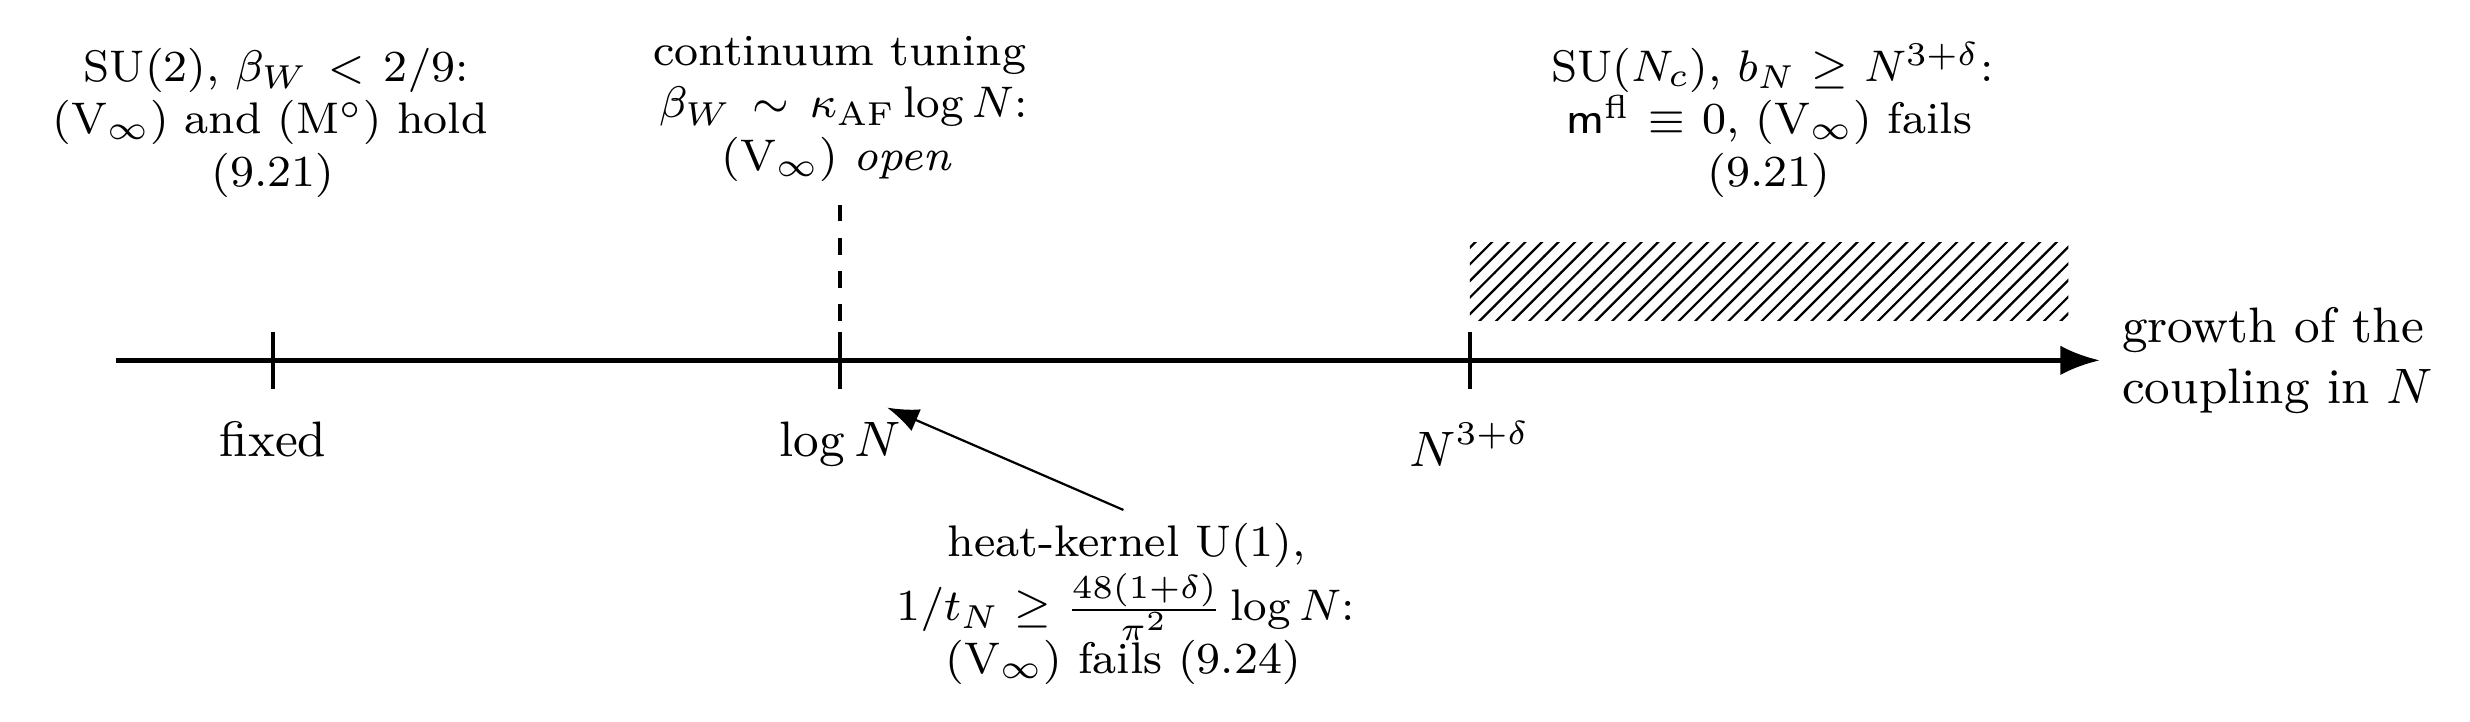
\includegraphics[width=444.6bp]{figures/fig14.png}
\caption{What is known about the vortex rate \textup{(V$_\infty$)} as a function of how fast the coupling grows with the cutoff $N$. At fixed strong coupling it holds; once the coupling grows like $N^{3+\delta}$ the flux energy of every cube of fixed physical size vanishes in physical units; the abelian heat-kernel theory violates it already at a logarithmic coupling of slope $48(1+\delta)/\pi^2$. The continuum tuning of $\SU(N_c)$, of slope $\kappa_{\mathrm{AF}}=11C_A/(24\pi^2)$, lies in the open region.}
\label{fig:vortex}
\end{figure}

The heat-kernel $\U(1)$ theory has a connected compact gauge group, a positive-definite class weight, reflection positivity and the centre grading of \cref{lem:centre-operators}, and along the family of \cref{prop:abelian-vortex} its coupling $1/t_N\ge(48(1+\delta)/\pi^2)\log N$ grows only logarithmically in the cutoff. So no argument from these properties, nor from connectedness of the gauge group with a logarithmic tuning, gives \textup{(V$_\infty$)}; with \cref{prop:no-vortex-comparison} and \cref{rem:neutral-connectedness}, a proof of \textup{(V$_\infty$)} for $\SU(N_c)$ must use the non-abelian structure of the group, as \Mcirc{} must (\cref{thm:abelian}). By \cref{cor:BF-vortex} it must also be posed at a scale at which small-field control has ended. Whether \textup{(V$_\infty$)} holds for the Wilson theory along the continuum tuning remains open.

\subsection{Charged decorrelation at physical times}\label{sec:timed-decorrelation}

The one-step Cheeger inequality \eqref{eq:charged-cheeger} brackets $1-r^{\mathrm{fl}}$ between $\frac12h^2$ and $2h$, and on cubes of physical side $2t$ the two ends correspond to $h\gtrsim N^{-1/2}$ and $h\gtrsim N^{-1}$. Passing to the joint law of two slices a physical time apart removes this loss: the flux condition \textup{(V$_\infty$)} becomes a lower bound of order one on an isoperimetric constant (\cref{thm:timed-poincare}). A sufficient condition in the form of a coupling of the slice process with its centre image follows (\cref{prop:overlap-criterion}). An abelian factor of the gauge group that carries part of $C$ violates \textup{(V$_\infty$)} under a logarithmic tuning of that factor alone (\cref{prop:abelian-factor}), while the deformability of the centre flip through symmetries of the slice action does not distinguish $\U(1)$ from non-abelian groups (\cref{lem:link-multiplications}).

Throughout, the notation is that of \cref{thm:charged-poincare}. For a spatial torus $s$ and an integer $n\ge1$ put
\begin{gather*}
\nu^{(n)}_s(\dd Q\,\dd Q')=\Omegazero(Q)R_s^n(Q,Q')\Omegazero(Q')\dd Q\,\dd Q',\\
\mathcal E^{(n)}_s(F)=\tfrac12\int\abs{F(Q)-F(Q')}^2\nu^{(n)}_s(\dd Q\,\dd Q'),
\end{gather*}
and, for a nonzero character $e$ of $C^3$ with values $\pm1$, $h^{(n)}_e(s)=\inf_A\nu^{(n)}_s(A\times A^c)/\pi_s(A)$, the infimum over the $e$-free sets $A$. Thus $\nu^{(1)}_s=\nu_s$ and $h^{(1)}_e=h_e$.

\begin{theorem}[charged Poincar\'e constant at time separation $n$]\label{thm:timed-poincare}
\begin{enumerate}[label=\textup{(\alph*)},leftmargin=*]
\item Let $s$ be a spatial torus and $n\ge1$. For every character $e$ of $C^3$, $1-\norm{P_eR_s}^n$ is the infimum of $\mathcal E^{(n)}_s(F)/\pi_s(\abs F^2)$ over the bounded measurable $F$ with $F\circ\zeta^k=e(k)F$ for all $k$ and $\pi_s(\abs F^2)>0$; $1-r^{\mathrm{fl}}(s)^n$ is the same infimum over the bounded $F\ne0$ with $\sum_kF\circ\zeta^k=0$; and if $e\ne0$ takes only the values $\pm1$,
\begin{equation}\label{eq:timed-cheeger}
\tfrac12h^{(n)}_e(s)^2\le1-\norm{P_eR_s}^n\le2h^{(n)}_e(s).
\end{equation}
For the Wilson theory, $\int F(Q)H(Q')\,\nu^{(n)}_s=\mu^0_s(F\,\tau_nH)$ for bounded slice functions $F,H$: $\nu^{(n)}_s$ is the joint law of the slices at the times $0$ and $n$ in the slice limit.
\item For a family of systems of \cref{sec:centre} and $\tau,t>0$ let $\Pi_\tau(t)=\liminf_{p\to\infty}\liminf_{N\to\infty}\bigl(1-r^{\mathrm{fl}}_{N,p}(\cube{\lfloor Nt\rfloor})^{\lfloor N\tau\rfloor}\bigr)$. Then
\[
\Pi_\tau(t)=1-e^{-\tau\,\mathsf m^{\mathrm{fl}}(t)} .
\]
Hence \textup{(V$_\infty$)} holds if and only if $\liminf_{t\to\infty}\Pi_\tau(t)>0$ for one $\tau>0$, and if and only if this holds for every $\tau>0$.
\item Let $G=\SU(2)$ with the Wilson weight and $C=\{\pm1\}$, let $h^{(n)}(s)=\min_{e\ne0}h^{(n)}_e(s)$ and $H_\tau(t)=\liminf_p\liminf_Nh^{(\lfloor N\tau\rfloor)}_{N,p}(\cube{\lfloor Nt\rfloor})$. Then
\[
\tfrac12H_\tau(t)^2\le1-e^{-\tau\,\mathsf m^{\mathrm{fl}}(t)}\le2H_\tau(t),
\]
so \textup{(V$_\infty$)} holds if and only if $\liminf_{t\to\infty}H_\tau(t)>0$ for one, equivalently every, $\tau>0$. Moreover $1-r^{\mathrm{fl}}(s)^n\le2\,\mu^0_s(\Tr P_j\cdot\tau_n\Tr P_j<0)$ for every $j$, and
\[
\liminf_{p\to\infty}\liminf_{N\to\infty}\mu^0_{\cube{\lfloor Nt\rfloor}}\bigl(\Tr P_j\cdot\tau_{\lfloor N\tau\rfloor}\Tr P_j<0\bigr)\ge\tfrac12\bigl(1-e^{-\tau\,\mathsf m^{\mathrm{fl}}(t)}\bigr).
\]
\end{enumerate}
\end{theorem}

\begin{proof}
(a) By \cref{lem:transfer-matrix}(i) and \cref{lem:centre-operators}(a), $P_eR_s^n=(P_eR_s)^n\ge0$, so $\norm{P_eR_s^n}=\norm{P_eR_s}^n$, and the norm of $R_s^n$ on $\Kspace^{\ne}$ is $r^{\mathrm{fl}}(s)^n$. The kernel of $R_s^n$ is continuous, strictly positive and symmetric, $R_s^n\Omegazero=\Omegazero$, and $R_s^n$ commutes with every $z^k$. Hence $\nu^{(n)}_s$ is a symmetric probability measure with marginals $\pi_s$, and $\nu^{(n)}_s$ and $\pi_s$ are invariant under the simultaneous action of $\zeta^k$. These are the only properties of $R_s$ and $\nu_s$ used in the proof of \cref{thm:charged-poincare}(a),(b), besides the nonnegativity of $R_s$ on $\Kspace^e_s$, which $R_s^n$ shares; that proof with $R_s^n$ and $\nu^{(n)}_s$ in place of $R_s$ and $\nu_s$ gives the first three claims. The last is \eqref{eq:fp-slice} with $s=n$, valid on every spatial torus (proof of \cref{lem:fp-slice}(a)).

(b) Fix $p$ and $t$, put $x_N=N(-\log r^{\mathrm{fl}}_{N,p}(\cube{\lfloor Nt\rfloor}))\in[0,\infty]$, $n_N=\lfloor N\tau\rfloor$ and $c_N=n_N/N\to\tau$. Then $1-r^{\mathrm{fl}}_{N,p}(\cube{\lfloor Nt\rfloor})^{n_N}=\phi(c_Nx_N)$ with $\phi(y)=1-e^{-y}$, continuous and nondecreasing on $[0,\infty]$. For such $\phi$, $\liminf\phi(y_N)=\phi(\liminf y_N)$, and $\liminf c_Nx_N=\tau\liminf x_N$ since $c_N\to\tau\in(0,\infty)$; so $\liminf_N\phi(c_Nx_N)=\phi(\tau\liminf_Nx_N)$, and the same argument applies to $\liminf_p$. If $\mathsf m^{\mathrm{fl}}_\infty=m>0$, then $\mathsf m^{\mathrm{fl}}(t)\ge m/2$ and $\Pi_\tau(t)\ge1-e^{-\tau m/2}$ for large $t$; if $\Pi_\tau(t)\ge\delta>0$ for large $t$, then $\mathsf m^{\mathrm{fl}}(t)\ge-\tau^{-1}\log(1-\delta)$ there.

(c) As $r^{\mathrm{fl}}=\max_{e\ne0}\norm{P_eR_s}$ (\cref{thm:charged-poincare}(c)), taking the minimum over $e\ne0$ in \eqref{eq:timed-cheeger} gives $\frac12h^{(n)}(s)^2\le1-r^{\mathrm{fl}}(s)^n\le2h^{(n)}(s)$. Limits inferior are monotone and commute with $y\mapsto\frac12y^2$ on $[0,\infty)$, and (b) gives the first display and the equivalence. For the Polyakov loop let $e^{(j)}(k)=(-1)^{k_j}$ and $A=\{\Tr P_j>0\}$. As in the proof of \cref{thm:charged-poincare}(c), $A$ is $e^{(j)}$-free, $\pi_s(A)=\frac12$ and $A^c=\sigma A$ up to a null set; by symmetry of $\nu^{(n)}_s$ and the identity of (a) applied to $1_A\otimes1_{\sigma A}+1_{\sigma A}\otimes1_A$, $2\nu^{(n)}_s(A\times A^c)=\mu^0_s(\Tr P_j\cdot\tau_n\Tr P_j<0)$. The upper bound in \eqref{eq:timed-cheeger} gives $1-r^{\mathrm{fl}}(s)^n\le1-\norm{P_{e^{(j)}}R_s}^n\le4\nu^{(n)}_s(A\times A^c)$, and (b) gives the last display.
\end{proof}

Under \textup{(V$_\infty$)} the sign of the trace of every spatial holonomy winding the cube therefore decorrelates in physical time: it flips between slices a physical time $\tau$ apart with probability at least $\frac12(1-e^{-\tau\mathsf m^{\mathrm{fl}}_\infty/2})$ for large $t$. In the single-step form of \cref{thm:charged-poincare}(c) the necessary condition $h\gtrsim N^{-1}$ and the sufficient condition $h\gtrsim N^{-1/2}$ differ; at the separation $\lfloor N\tau\rfloor$ both are bounds of order one.

For $n\ge1$ the kernel $\mathsf q_n(Q,\dd Q')=R_s^n(Q,Q')\Omegazero(Q')\Omegazero(Q)^{-1}\dd Q'$ is a Markov kernel with $\nu^{(n)}_s(\dd Q\,\dd Q')=\pi_s(\dd Q)\mathsf q_n(Q,\dd Q')$: for the Wilson theory, $\mathsf q_n(Q,\cdot)$ is the law of the slice at time $n$ given the slice $Q$ at time $0$. For $k\in C^3$ write $(\zeta^k)_*\mu=\mu\circ\zeta^{-k}$, $\norm{\mu-\mu'}_{\mathrm{TV}}=\sup_B\abs{\mu(B)-\mu'(B)}$, and
\[
\mathsf d^k_n(Q)=\bigl\Vert\mathsf q_n(Q,\cdot)-(\zeta^k)_*\mathsf q_n(Q,\cdot)\bigr\Vert_{\mathrm{TV}},\qquad \mathsf d_n(s)=\max_{k\ne1}\sup_Q\mathsf d^k_n(Q).
\]
By the computation in the proof of \cref{lem:centre-operators}(b), the density ratio $R_s^n(Q,\zeta^kQ')/R_s^n(Q,Q')$ is the ratio of the integrals over the slab $[0,n]$ with boundary slices $Q$ and $Q'$, with and without a centre twist on one $(j,4)$-stack for each $j$ with $k_j\ne1$; so $\mathsf d^k_n$ measures how far such a twist across the slab is from being screened, uniformly in the boundary data.

\begin{proposition}[an overlap criterion]\label{prop:overlap-criterion}
Let $s$ be a spatial torus and $n\ge1$.
\begin{enumerate}[label=\textup{(\alph*)},leftmargin=*]
\item If $e$ is a character of $C^3$ and $e(k)\ne1$, then $\norm{P_eR_s}^n\le2\abs{1-e(k)}^{-1}\sup_Q\mathsf d^k_n(Q)$. For $C=\{\pm1\}$, $r^{\mathrm{fl}}(s)^n\le\mathsf d_n(s)$.
\item For integers $1\le a<n$ and every $Q$, $\mathsf d^k_n(Q)\le\int\mathsf q_a(Q,\dd Q'')\,\mathsf d^k_{n-a}(Q'')$ and $\mathsf d^k_n(Q)\le\mathsf d^k_a(Q)$; in particular $\sup_Q\mathsf d^k_n(Q)$ is nonincreasing in $n$, and for every measurable set $\mathcal G$, $\mathsf d^k_n(Q)\le\mathsf q_a(Q,\mathcal G^c)+\sup_{\mathcal G}\mathsf d^k_{n-a}$.
\item Let $Z_{N,p}$ be a family of systems of \cref{sec:centre} with $C=\{\pm1\}$, and suppose there are $\tau>0$, $\delta\in(0,1)$ and $t_*$ such that $\limsup_p\limsup_N\mathsf d_{\lfloor N\tau\rfloor}(\cube{\lfloor Nt\rfloor})\le1-\delta$ for every $t\ge t_*$. Then $\mathsf m^{\mathrm{fl}}(t)\ge-\tau^{-1}\log(1-\delta)$ for $t\ge t_*$, and \textup{(V$_\infty$)} holds.
\end{enumerate}
\end{proposition}

\begin{proof}
(a) Let $\omega=e(k)$, let $F$ be bounded with $F\circ\zeta^{k'}=e(k')F$ for all $k'$, and $h=F\Omegazero$. Put $I(Q)=\int F(Q')R_s^n(Q,Q')\Omegazero(Q')\dd Q'$ and $J(Q)=\int F(Q')R_s^n(Q,\zeta^kQ')\Omegazero(Q')\dd Q'$. The substitution $Q'\mapsto\zeta^kQ'$ preserves Haar measure, and $\Omegazero\circ\zeta^k=\Omegazero$, so $I=\omega J$ and $I-J=(1-\bar\omega)I$. With $\kappa(Q,Q')=\Omegazero(Q)\abs{R_s^n(Q,Q')-R_s^n(Q,\zeta^kQ')}\Omegazero(Q')$ and $2ab\le a^2+b^2$,
\begin{align*}
\abs{\ip h{R_s^nh}}&=\Bigl\lvert\int\overline{F(Q)}\Omegazero(Q)I(Q)\dd Q\Bigr\rvert\le\frac1{\abs{1-\omega}}\int\!\!\int\abs{F(Q)}\abs{F(Q')}\kappa(Q,Q')\dd Q\dd Q'\\
&\le\frac1{2\abs{1-\omega}}\Bigl(\int\abs{F(Q)}^2\!\!\int\kappa(Q,Q')\dd Q'\dd Q+\int\abs{F(Q')}^2\!\!\int\kappa(Q,Q')\dd Q\dd Q'\Bigr).
\end{align*}
For $m\in C^3$ the measure with density $R_s^n(Q,\zeta^mQ')\Omegazero(Q')/\Omegazero(Q)$ is $(\zeta^{-m})_*\mathsf q_n(Q,\cdot)$, and the total variation distance is invariant under applying $(\zeta^m)_*$ to both measures; so $\int\kappa(Q,Q')\dd Q'=2\Omegazero(Q)^2\mathsf d^k_n(Q)$. The kernel $R_s^n$ is symmetric and invariant under the simultaneous action of $\zeta^k$, so $R_s^n(Q,\zeta^kQ')=R_s^n(Q',\zeta^{-k}Q)$ and $\int\kappa(Q,Q')\dd Q=2\Omegazero(Q')^2\mathsf d^{-k}_n(Q')=2\Omegazero(Q')^2\mathsf d^k_n(Q')$. Hence $\abs{\ip h{R_s^nh}}\le2\abs{1-\omega}^{-1}\sup_Q\mathsf d^k_n(Q)\norm h^2$. The operator $P_eR_s^n$ is self-adjoint on $\Kspace^e_s$, and the vectors $h$ of this form are dense there (proof of \cref{thm:charged-poincare}(a)); so $\norm{P_eR_s}^n=\norm{P_eR_s^n}$ satisfies the claimed bound. For $C=\{\pm1\}$ every $e\ne0$ has some $k$ with $e(k)=-1$, and $r^{\mathrm{fl}}=\max_{e\ne0}\norm{P_eR_s}$.

(b) $R_s^n=R_s^aR_s^{n-a}$ gives $\mathsf q_n(Q,\cdot)=\int\mathsf q_a(Q,\dd Q'')\mathsf q_{n-a}(Q'',\cdot)$, and the invariance of the kernels gives $(\zeta^k)_*\mathsf q_b(Q'',\cdot)=\mathsf q_b(\zeta^kQ'',\cdot)$, so that $(\zeta^k)_*$ commutes with the action of $\mathsf q_b$ on measures. The first inequality follows from the joint convexity of the total variation distance, the second from its contraction under the Markov kernel $\mathsf q_{n-a}$ applied to $\mathsf q_a(Q,\cdot)$ and $(\zeta^k)_*\mathsf q_a(Q,\cdot)$, and the last by splitting the first integral over $\mathcal G$ and $\mathcal G^c$ and using $\mathsf d^k\le1$.

(c) By (a), $1-r^{\mathrm{fl}}(s)^n\ge1-\mathsf d_n(s)$. Taking $\liminf_N$ and $\liminf_p$ on the cube $\cube{\lfloor Nt\rfloor}$ with $n=\lfloor N\tau\rfloor$, \cref{thm:timed-poincare}(b) gives $1-e^{-\tau\mathsf m^{\mathrm{fl}}(t)}\ge\delta$ for $t\ge t_*$.
\end{proof}

The hypothesis of (c) asks that from every slice,\footnote{Since $(\zeta^k)_*\mathsf q_n(Q,\cdot)=\mathsf q_n(\zeta^kQ,\cdot)$, the quantity $\sup_Q\mathsf d^k_n(Q)$ is the Dobrushin coefficient $\sup_{Q,Q'}\norm{\mathsf q_n(Q,\cdot)-\mathsf q_n(Q',\cdot)}_{\mathrm{TV}}$ of $\mathsf q_n$ restricted to the pairs $Q'=\zeta^kQ$. Part (a) is the analogue, on the centre-charged sectors, of the bound of every nontrivial eigenvalue of a Markov kernel by its Dobrushin coefficient: charged functions are odd under $\zeta^k$, so only these pairs enter.} after a fixed physical time, the slice process gives comparable weight to each configuration and its centre images; by (b) it suffices that the process enters a set $\mathcal G$ of slices within a time $a$ from every start, and that the overlap holds uniformly from $\mathcal G$. It is not known to be necessary: \textup{(V$_\infty$)} controls $\mathsf q_n$ on charged functions in $L^2(\pi_s)$, not uniformly in the starting slice. Along the $\U(1)$ family of \cref{prop:abelian-vortex}, $\mathsf m^{\mathrm{fl}}\equiv0$, so $1-\mathsf d_{\lfloor N\tau\rfloor}(\cube{\lfloor Nt\rfloor})\le1-r^{\mathrm{fl}}(\cube{\lfloor Nt\rfloor})^{\lfloor N\tau\rfloor}$ has limit inferior $0$ by (a) and \cref{thm:timed-poincare}(b), and the hypothesis fails there.

\begin{proposition}[an abelian factor carrying the centre]\label{prop:abelian-factor}
Let $H\subset\U(N_0)$ be closed, $G=H\times\U(1)\subset\U(N_0+1)$ embedded block-diagonally, $f=f^H\otimes p_t$ with $f^H\in\Fclass(H)$ and $t>0$, and $C$ a finite subgroup of the centre $Z(H)\times\U(1)$ whose projection $C_1$ to $\U(1)$ is not $\{1\}$. Then $r^{\mathrm{fl}}(s)\ge r^{\mathrm{fl}}_1(s)$ for every spatial torus $s$, where $r^{\mathrm{fl}}_1$ is computed in the heat-kernel $\U(1)$ system at time $t$ with the group $C_1$. Consequently, if $0<t_N\le\pi^2/(48(1+\delta)\log N)$ for some $\delta>0$ and all large $N$, every family of these systems with $f_{N,p}=f^H_{N,p}\otimes p_{t_N}$ has $\mathsf m^{\mathrm{fl}}\equiv0$, whatever the weights $f^H_{N,p}$: \textup{(V$_\infty$)} and \Mcirc{} fail along it.
\end{proposition}

\begin{proof}
The weight $f$ is a continuous positive class function, and its coefficient against the irreducible representation $\lambda\otimes(g\mapsto g^m)$ of $G$ is $f^H_\lambda e^{-tm^2/2}\ge0$; so $f\in\Fclass(G)$. All plaquette and temporal variables of $G$ are pairs, and Haar measure on $G^{\Lambda_s}$ is the product measure, so the kernel \eqref{eq:cg-kernel} factorises and $\TT_s=\TT^H_s\otimes\TT^1_s$ on $L^2(H^{E_s})\otimes L^2(\U(1)^{E_s})$. Its largest eigenvalue is $\lzero^H\lzero^1$ with the positive eigenvector $\Omegazero^H\otimes\Omegazero^1$, which is therefore the ground state (\cref{lem:transfer-matrix}(ii)), and $R_s=R^H_s\otimes R^1_s$. For $k=(k^H,k^1)\in C^3$ the flip $\zeta^k$ acts on both components, so $z^k=z^{k^H}\otimes z^{k^1}$, and $z^{k^H}\Omegazero^H=\Omegazero^H$ by \cref{lem:centre-operators}(a) for the $H$ system with the projection of $C$ to $Z(H)$. Let $e_1$ be a character of $C_1^3$ with $e_1\ne0$. The operator $P_{e_1}R^1_s$ is compact, self-adjoint and nonnegative, so if $\norm{P_{e_1}R^1_s}>0$ it has a unit eigenvector $h_1\in\Kspace^{e_1}$ with this eigenvalue. Then $z^k(\Omegazero^H\otimes h_1)=e_1(k^1)\,\Omegazero^H\otimes h_1$, and $e:k\mapsto e_1(k^1)$ is a nonzero character of $C^3$ because $C^3\to C_1^3$ is onto; and $R_s(\Omegazero^H\otimes h_1)=\norm{P_{e_1}R^1_s}\,\Omegazero^H\otimes h_1$. Hence $r^{\mathrm{fl}}(s)\ge\norm{P_eR_s}\ge\norm{P_{e_1}R^1_s}$, and maximising over $e_1$ gives the inequality. For the family, the proof of \cref{prop:abelian-vortex} with $C_1$ gives $N(-\log r^{\mathrm{fl}}_1(\cube{\lfloor N\tau\rfloor}))\le39t_NN/\lfloor N\tau\rfloor\to0$ for every $\tau>0$, so $\mathsf m^{\mathrm{fl}}\equiv0$, and \Mcirc{} fails by \cref{thm:sector-criterion}.
\end{proof}

If instead $C\subset H\times\{1\}$, then $r^{\mathrm{fl}}(s)=r^{\mathrm{fl}}_H(s)$ because $\norm{R^1_s}=1$, as in \cref{prop:no-residue-control}(a), and the abelian factor is invisible. If $H$ has no nontrivial continuous character, for instance $H=\SU(N_0)$, the condition $C\subset H\times\{1\}$ says that every continuous character of $G$ is trivial on $C$. The next lemma shows that the mechanism of \cref{prop:abelian-vortex} is not the deformability of the centre flip through symmetries of the slice action.

\begin{lemma}[link multiplications preserving the slice action]\label{lem:link-multiplications}
Let $G\subset\U(N_c)$ be closed with $\int_Gg\dd g=0$, let $s$ be a spatial torus with all sides at least $3$, $S_s(Q)=\sum_p\ReTr Q_p$ over the plaquettes of $\Lambda_s$, $j\le3$, and $\Pi_j=\{(x,j):x_j=0\}$. For $u\in G^{\Pi_j}$ let $M_u$ multiply $Q_b$ on the right by $u_b$ for $b\in\Pi_j$. Then $S_s\circ M_u=S_s$ if and only if there is $c$ in the centre of $G$ with $u_b=c$ for every $b\in\Pi_j$.
\end{lemma}

\begin{proof}
For constant central $u$ this is the computation in the proof of \cref{lem:fp-slice}(b). Conversely, let $x_j=0$, $i\ne j$, $u=u_{(x,j)}$, $v=u_{(x+e_i,j)}$ and $Y=Q_{(x+e_j,i)}$. The plaquettes containing the link $(x+e_j,i)$ are the two $\{i,j\}$-plaquettes based at $x$ and $x+e_j$ and two plaquettes in the third coordinate plane; only the first contains links of $\Pi_j$, since the $j$-links of the second have $j$-coordinate $1\not\equiv0$ and the last two contain no $j$-link. Since $\ReTr$ is invariant under inversion and cyclic permutation, $S_s(M_uQ)-S_s(Q)$ equals $\ReTr\bigl(Y(v^*Wu-W)\bigr)$ plus terms not depending on $Y$, with $W=Q^*_{(x+e_i,j)}Q^*_{(x,i)}Q_{(x,j)}$. So $Y\mapsto\ReTr(YM)$, $M=v^*Wu-W$, is constant on $G$, and its Haar average is $0$. Let $V$ be the real linear span of $G$; it is closed under adjoints, $M\in V$, and $\ReTr(A^*B)$ is an inner product on $V$; as $\ReTr(A^*M)=0$ for all $A\in G$, $M=0$. Since $W$ ranges over $G$ as $Q_{(x,i)}$ does, $v^*Wu=W$ for all $W\in G$: $W=1$ gives $u=v$, and then $u$ is central. The plane $x_j=0$ is connected by the steps $\pm e_i$, $i\ne j$, so $u$ is constant.
\end{proof}

For $\SU(N_c)$ the maps $M_u$ preserving $S_s$ are therefore the finitely many central flips, and no flip $\zeta^c_j$ with $c\ne1$ is joined to the identity through such symmetries; for $\U(1)$ the flip $\zeta_j^{-1}$ is, by the flips $\zeta_j^{e^{i\varphi}}=M_{e^{i\varphi}}$ with $\varphi\in[0,\pi]$, and the flux sector used in the proof of \cref{prop:abelian-vortex} is the charge-one eigenspace of this one-parameter group. The same deformation exists for $G=\U(2)$ and $C=\{\pm1\}$, where every continuous character of $G$ is a power of the determinant and is trivial on $C$, so neither \cref{prop:abelian-vortex} nor \cref{prop:abelian-factor} applies; whether \textup{(V$_\infty$)} holds there is not decided here. The property used in \cref{prop:abelian-factor} is the existence of a character of the gauge group that is nontrivial on $C$; the connectedness of the centre, which $\U(2)$ shares with $\U(1)$, is not used. Whether \textup{(V$_\infty$)} holds for the $\SU(2)$ Wilson theory along the continuum tuning remains open; by \cref{thm:timed-poincare} it is equivalent to a lower bound of order one on the charged isoperimetric constant of the joint law of two slices a fixed physical time apart, and by \cref{prop:overlap-criterion} it follows from a uniform overlap of the slice process with its centre images at a fixed physical time.

\subsection{Averaged overlap and the neutral gap}\label{sec:averaged-overlap}

The criterion of \cref{prop:overlap-criterion} asks for an overlap of the slice process with its centre images that is uniform in the starting slice. In the presence of the neutral gap, the overlap averaged over the starting slice suffices (\cref{thm:averaged-overlap}). Conversely, the averaged overlap is controlled by the flux energy, at the price of the thermal trace at a shorter time (\cref{prop:overlap-converse}). Along a family with $C=\{\pm1\}$, \Mcirc{} is equivalent to the vanishing of the neutral free energy together with the vanishing of the averaged overlap defect at a fixed aspect ratio, and a defect bounded away from $1$ at one fixed physical time suffices (\cref{thm:overlap-criteria}). None of these statements proves \textup{(V$_\infty$)} along the continuum tuning.

The notation is that of \cref{prop:overlap-criterion}. For a bounded measurable function $g$ on $G^{E_s}$ put $(\mathsf q_ng)(Q)=\int g(Q')\,\mathsf q_n(Q,\dd Q')$. Then $R_s^n(g\Omegazero)=(\mathsf q_ng)\Omegazero$, so the unitary map $g\mapsto g\Omegazero$ from $L^2(\pi_s)$ onto $\Kspace_s$ carries $\mathsf q_n$ to $R_s^n$: $\mathsf q_n$ is self-adjoint and nonnegative on $L^2(\pi_s)$, $\mathsf q_{n+n'}=\mathsf q_n\mathsf q_{n'}$, and $\pi_s\mathsf q_n=\pi_s$. Let $L^2_0(\pi_s)$ be the subspace of the functions invariant under every $\zeta^k$. It is carried onto $\Kspace^0_s$ and the constants onto $\C\Omegazero$; since $R_s$ is compact and nonnegative on $\Kspace^0_s$ with the eigenvalue $1$ belonging to $\Omegazero$, and $r_1^0(s)$ is its next eigenvalue with multiplicity, the norm of $\mathsf q_n$ on the orthogonal complement of the constants in $L^2_0(\pi_s)$ is $r_1^0(s)^n$. For $k\in C^3$ and $n\ge1$ put
\[
\mathsf D^k_n(s)=\int\mathsf d^k_n\,\dd\pi_s,\qquad \mathsf D_n(s)=\max_{k\ne1}\mathsf D^k_n(s).
\]
The measure $\nu^{(n)}_s$ is $\pi_s(\dd Q)\,\mathsf q_n(Q,\dd Q')$, and $(1\times\zeta^k)_*\nu^{(n)}_s$ is $\pi_s(\dd Q)\,(\zeta^k)_*\mathsf q_n(Q,\dd Q')$. With respect to Haar measure they have the densities $\Omegazero(Q)R_s^n(Q,Q')\Omegazero(Q')$ and $\Omegazero(Q)R_s^n(Q,\zeta^{-k}Q')\Omegazero(Q')$, so
\begin{gather*}
\mathsf D^k_n(s)=\bigl\Vert\nu^{(n)}_s-(1\times\zeta^k)_*\nu^{(n)}_s\bigr\Vert_{\mathrm{TV}},\\
1-\mathsf D^k_n(s)=\int\!\!\int\Omegazero(Q)\min\bigl\{R_s^n(Q,Q'),R_s^n(Q,\zeta^{-k}Q')\bigr\}\Omegazero(Q')\dd Q\dd Q' .
\end{gather*}
For the Wilson theory $\mathsf D^k_n(s)$ is therefore the total variation distance between the joint law of the slices $Q_0$, $Q_n$ at the times $0$ and $n$ in the slice limit and the joint law of $Q_0$ and $\zeta^kQ_n$ (\cref{thm:timed-poincare}(a)); the density ratio $\rho^k_n(Q,Q')=R_s^n(Q,\zeta^{-k}Q')/R_s^n(Q,Q')$ is the ratio of slab integrals described before \cref{prop:overlap-criterion}, with $-k$ in place of $k$; its integral against $\nu^{(n)}_s$ is $\ip{\Omegazero}{R_s^nz^{k}\Omegazero}=1$, and $1-\mathsf D^k_n(s)=\int\min\{1,\rho^k_n\}\dd\nu^{(n)}_s$. By \cref{prop:overlap-criterion}(b) and $\pi_s\mathsf q_a=\pi_s$, $\mathsf D^k_n(s)$ is nonincreasing in $n$. The function $\mathsf d^k_n$ is measurable, and it is invariant under every $\zeta^{k'}$: $\mathsf q_n(\zeta^{k'}Q,\cdot)=(\zeta^{k'})_*\mathsf q_n(Q,\cdot)$ by the invariance of the kernel, and $(\zeta^{k'})_*$ commutes with $(\zeta^k)_*$ and preserves total variation distances.

\begin{theorem}[averaged overlap]\label{thm:averaged-overlap}
Let $s$ be a spatial torus and $m,a\ge1$ integers.
\begin{enumerate}[label=\textup{(\alph*)},leftmargin=*]
\item If $e$ is a character of $C^3$ and $e(k)\ne1$, then
\[
\norm{P_eR_s}^{m+2a}\le\frac2{\abs{1-e(k)}}\Bigl(r_1^0(s)^{2a}+\bigl(1-r_1^0(s)^{2a}\bigr)\mathsf D^k_m(s)\Bigr).
\]
\item If $C=\{\pm1\}$, then
\begin{equation}\label{eq:averaged-overlap}
1-r^{\mathrm{fl}}(s)^{m+2a}\ge\bigl(1-\mathsf D_m(s)\bigr)\bigl(1-r_1^0(s)^{2a}\bigr),
\end{equation}
and for every measurable set $\mathcal G$ of slices, with $\mathsf d^\ast_m(Q)=\max_{k\ne1}\mathsf d^k_m(Q)$,
\[
1-r^{\mathrm{fl}}(s)^{m+2a}\ge\pi_s(\mathcal G)\Bigl(1-\sup_{\mathcal G}\mathsf d^\ast_m\Bigr)\bigl(1-r_1^0(s)^{2a}\bigr).
\]
\end{enumerate}
\end{theorem}

\begin{proof}
Inner products and norms are those of $L^2(\pi_s)$. Write $\omega=e(k)$, $\varepsilon=r_1^0(s)^{2a}$ and $c_\omega=2\abs{1-\omega}^{-1}$.

\emph{Step 1: a weighted form of \cref{prop:overlap-criterion}(a).} Let $g$ be bounded with $g\circ\zeta^k=\omega g$. Then
\[
\abs{\ip g{\mathsf q_mg}}\le c_\omega\int\mathsf d^k_m\abs g^2\dd\pi_s .
\]
Indeed, let $\lambda_Q=\abs{\mathsf q_m(Q,\cdot)-(\zeta^k)_*\mathsf q_m(Q,\cdot)}$, a measure of mass $2\mathsf d^k_m(Q)$. Since $g\circ\zeta^k=\omega g$,
\begin{align*}
(1-\omega)(\mathsf q_mg)(Q)&=\int g(Q')\,\mathsf q_m(Q,\dd Q')-\int g(\zeta^kQ')\,\mathsf q_m(Q,\dd Q')\\
&=\int g\dd\bigl(\mathsf q_m(Q,\cdot)-(\zeta^k)_*\mathsf q_m(Q,\cdot)\bigr),
\end{align*}
hence $\abs{(\mathsf q_mg)(Q)}\le\abs{1-\omega}^{-1}\int\abs g\dd\lambda_Q$, and by $2\abs{xy}\le\abs x^2+\abs y^2$
\[
\abs{\ip g{\mathsf q_mg}}\le\frac1{2\abs{1-\omega}}\Bigl(\int\abs{g(Q)}^2\lambda_Q(G^{E_s})\,\pi_s(\dd Q)+\int\!\!\int\abs{g(Q')}^2\lambda_Q(\dd Q')\,\pi_s(\dd Q)\Bigr).
\]
The first integral is $\int2\mathsf d^k_m\abs g^2\dd\pi_s$. The measure $\pi_s(\dd Q)\lambda_Q(\dd Q')$ has the density $\Omegazero(Q)\abs{R_s^m(Q,Q')-R_s^m(Q,\zeta^{-k}Q')}\Omegazero(Q')$, and $R_s^m(Q,\zeta^{-k}Q')=R_s^m(Q',\zeta^kQ)$ by the symmetry and the invariance of the kernel; so its second marginal is $2\mathsf d^{-k}_m(Q')\pi_s(\dd Q')$, and $\mathsf d^{-k}_m=\mathsf d^k_m$ because the total variation distance is invariant under applying $(\zeta^k)_*$ to both measures. This gives the claim.

\emph{Step 2: the neutral sector.} Let $B$ be a measurable set invariant under every $\zeta^{k'}$, and $\theta(B)=\varepsilon+(1-\varepsilon)\pi_s(B)$. Then $\int_B\abs{\mathsf q_aH}^2\dd\pi_s\le\theta(B)\norm H^2$ for every $H\in L^2_0(\pi_s)$. Indeed, $A=1_B\mathsf q_a$ maps $L^2_0(\pi_s)$ into itself, its adjoint there is $\mathsf q_a1_B$, and $\int_B\abs{\mathsf q_aH}^2\dd\pi_s=\norm{AH}^2\le\norm{AA^*}\norm H^2$ with $AA^*=1_B\mathsf q_{2a}1_B\ge0$. The norm of $AA^*$ on $L^2_0(\pi_s)$ is the supremum of $\ip K{\mathsf q_{2a}K}$ over the $K\in L^2_0(\pi_s)$ with $\norm K\le1$ that vanish off $B$. For such $K$ write $K=c+K_\perp$ with $c=\int K\dd\pi_s$; then $\abs c^2\le\pi_s(B)\norm K^2$ by the Cauchy--Schwarz inequality, and, as $\mathsf q_{2a}1=1$ and $\mathsf q_{2a}$ is self-adjoint,
\[
\ip K{\mathsf q_{2a}K}=\abs c^2+\ip{K_\perp}{\mathsf q_{2a}K_\perp}\le\abs c^2+\varepsilon\bigl(\norm K^2-\abs c^2\bigr)\le\theta(B)\norm K^2 .
\]

\emph{Step 3.} Let $F$ be bounded with $F\circ\zeta^{k'}=e(k')F$ for every $k'$, and $g=\mathsf q_aF$. Then $g$ is bounded, $g\circ\zeta^k=\omega g$ because $\mathsf q_a$ commutes with composition by $\zeta^k$, $\abs g\le\mathsf q_a\abs F$ pointwise because $\mathsf q_a(Q,\cdot)$ is a probability measure, and $\abs F\in L^2_0(\pi_s)$. Since $\mathsf q_{m+2a}=\mathsf q_a\mathsf q_m\mathsf q_a$ and $\mathsf q_a$ is self-adjoint, Step~1 gives
\[
\ip F{\mathsf q_{m+2a}F}=\ip g{\mathsf q_mg}\le c_\omega\int\mathsf d^k_m\abs g^2\dd\pi_s .
\]
For $0\le\mu<1$ the set $B_\mu=\{\mathsf d^k_m>\mu\}$ is invariant under every $\zeta^{k'}$, and Step~2 with $H=\abs F$ gives $\int_{B_\mu}\abs g^2\dd\pi_s\le\int_{B_\mu}\abs{\mathsf q_a\abs F}^2\dd\pi_s\le\theta(B_\mu)\norm F^2$. As $0\le\mathsf d^k_m\le1$, Fubini's theorem gives
\[
\int\mathsf d^k_m\abs g^2\dd\pi_s=\int_0^1\!\!\int_{B_\mu}\abs g^2\dd\pi_s\dd\mu\le\norm F^2\int_0^1\theta(B_\mu)\dd\mu=\bigl(\varepsilon+(1-\varepsilon)\mathsf D^k_m(s)\bigr)\norm F^2,
\]
because $\int_0^1\pi_s(B_\mu)\dd\mu=\int\mathsf d^k_m\dd\pi_s$. Finally $\ip F{\mathsf q_{m+2a}F}=\ip{F\Omegazero}{R_s^{m+2a}F\Omegazero}$, the operator $P_eR_s^{m+2a}$ is nonnegative on $\Kspace^e_s$, and the vectors $F\Omegazero$ are dense there (proof of \cref{thm:charged-poincare}(a)); so $\norm{P_eR_s}^{m+2a}=\norm{P_eR_s^{m+2a}}$ is the supremum of $\ip F{\mathsf q_{m+2a}F}/\norm F^2$ over these $F$, and (a) follows.

(b) For $C=\{\pm1\}$ every $e\ne0$ has some $k$ with $e(k)=-1$, so that $c_{e(k)}=1$, and $r^{\mathrm{fl}}(s)=\max_{e\ne0}\norm{P_eR_s}$. Part (a) gives $\norm{P_eR_s}^{m+2a}\le\varepsilon+(1-\varepsilon)\mathsf D_m(s)$ for every $e\ne0$, which is \eqref{eq:averaged-overlap}. The last claim follows from $\mathsf D_m(s)\le\int\mathsf d^\ast_m\dd\pi_s\le\pi_s(\mathcal G)\sup_{\mathcal G}\mathsf d^\ast_m+1-\pi_s(\mathcal G)$, as $\mathsf d^\ast_m\le1$.
\end{proof}

In the last form of (b) the set $\mathcal G$ needs only stationary probability bounded below; no condition is imposed on the time the slice process needs to reach $\mathcal G$, which is the condition of \cref{prop:overlap-criterion}(b). The mixing of the information that does not see the centre is supplied by the neutral sector, through Step~2.

\begin{proposition}[the converse up to a thermal trace]\label{prop:overlap-converse}
Let $s$ be a spatial torus, $n,a\ge1$ integers and $k\in C^3$. Then for every slice $Q$
\[
\mathsf d^k_{n+a}(Q)\le\frac{R_s^{2a}(Q,Q)^{1/2}}{\Omegazero(Q)}\,r^{\mathrm{fl}}(s)^n,\qquad \mathsf D^k_{n+a}(s)\le\Zs{s}{2a}^{1/2}\,r^{\mathrm{fl}}(s)^n .
\]
\end{proposition}

\begin{proof}
For bounded $h$ with $\abs h\le1$ put $u=h-h\circ\zeta^k$. Since $\int h\dd(\zeta^k)_*\mu=\int h\circ\zeta^k\dd\mu$, $\mathsf d^k_{n+a}(Q)=\frac12\sup_h\abs{(\mathsf q_{n+a}u)(Q)}$. The average of $u\circ\zeta^{k'}$ over $k'\in C^3$ vanishes, so $u\Omegazero\in(1-P_0)\Kspace_s$, and $\norm{\mathsf q_nu}_{L^2(\pi_s)}\le r^{\mathrm{fl}}(s)^n\norm u_{L^2(\pi_s)}\le2r^{\mathrm{fl}}(s)^n$. The measure $\mathsf q_a(Q,\cdot)$ has the density $\rho_Q(Q'')=R_s^a(Q,Q'')\Omegazero(Q)^{-1}\Omegazero(Q'')^{-1}$ with respect to $\pi_s$, and $\int\rho_Q^2\dd\pi_s=R_s^{2a}(Q,Q)\Omegazero(Q)^{-2}$ by the symmetry of the kernel. By the Cauchy--Schwarz inequality,
\[
\abs{(\mathsf q_{n+a}u)(Q)}=\Bigl\lvert\int\rho_Q\,\mathsf q_nu\dd\pi_s\Bigr\rvert\le2\,\frac{R_s^{2a}(Q,Q)^{1/2}}{\Omegazero(Q)}\,r^{\mathrm{fl}}(s)^n,
\]
which is the first bound. Integrating it against $\pi_s$ and using the Cauchy--Schwarz inequality with $\int\Omegazero^2\dd Q=1$,
\[
\mathsf D^k_{n+a}(s)\le r^{\mathrm{fl}}(s)^n\int\Omegazero(Q)R_s^{2a}(Q,Q)^{1/2}\dd Q\le r^{\mathrm{fl}}(s)^n\Bigl(\int R_s^{2a}(Q,Q)\dd Q\Bigr)^{1/2},
\]
and $\int R_s^{2a}(Q,Q)\dd Q=\int\!\!\int R_s^a(Q,Q'')^2\dd Q\dd Q''$ is the squared Hilbert--Schmidt norm of $R_s^a$, which is $\Tr R_s^{2a}=\Zs{s}{2a}$.
\end{proof}

So the averaged overlap defect and the flux energy determine each other up to two quantities that do not see the centre: the neutral gap, in \cref{thm:averaged-overlap}, and the thermal trace $\Zs{s}{2a}=\exp(\XT{s}{2a})$ at the thermal time $2a$, in \cref{prop:overlap-converse}. In physical units this reads as follows. For a family $(Z_{N,p})$ and $\tau,\alpha,t>0$ put
\[
\bar{\mathsf D}_\tau(t)=\limsup_{p\to\infty}\,\limsup_{N\to\infty}\,\mathsf D_{\lfloor N\tau\rfloor}\bigl(\cube{\lfloor Nt\rfloor}\bigr),\qquad \hat y_\alpha(t)=\limsup_{p\to\infty}\,\limsup_{N\to\infty}\,\XT{\cube{\lfloor Nt\rfloor}}{2\lfloor N\alpha\rfloor},
\]
both computed in $Z_{N,p}$: the averaged overlap defect after the physical time $\tau$ on the cube of physical side $2t$, and the free energy of that cube at the temperature $1/(2\alpha)$.

\begin{corollary}[averaged overlap in physical units]\label{cor:overlap-physical}
Let $(Z_{N,p})$ be a family of systems of \cref{sec:centre} with $C=\{\pm1\}$, and $\tau,\alpha,t>0$.
\begin{enumerate}[label=\textup{(\alph*)},leftmargin=*]
\item $1-e^{-(\tau+2\alpha)\mathsf m^{\mathrm{fl}}(t)}\ge\bigl(1-\bar{\mathsf D}_\tau(t)\bigr)\bigl(1-e^{-2\alpha\mathsf m^0(t)}\bigr)$.
\item If $\hat y_\alpha(t)<\infty$, then $\bar{\mathsf D}_{\tau+\alpha}(t)\le\exp\bigl(\tfrac12\hat y_\alpha(t)-\tau\,\mathsf m^{\mathrm{fl}}(t)\bigr)$.
\item If $\mathsf m^0_\infty>0$ and $\limsup_{t\to\infty}\bar{\mathsf D}_\tau(t)<1$ for some $\tau>0$, then \textup{(V$_\infty$)} holds: whenever $\mathsf m^0(t)\ge\Delta_0>0$ and $\bar{\mathsf D}_\tau(t)\le1-\delta$,
\[
\mathsf m^{\mathrm{fl}}(t)\ge-\frac1{\tau+2}\log\bigl(1-\delta(1-e^{-2\Delta_0})\bigr).
\]
If moreover $\liminf_{t\to\infty}y^0(t)<\infty$, then \Mcirc{} holds along the family.
\end{enumerate}
\end{corollary}

\begin{proof}
(a) Fix $p$ and $t$. For large $N$ put $m_N=\lfloor N\tau\rfloor\ge1$, $a_N=\lfloor N\alpha\rfloor\ge1$, $n_N=m_N+2a_N$ and $s=\cube{\lfloor Nt\rfloor}$; \eqref{eq:averaged-overlap} gives $1-r^{\mathrm{fl}}(s)^{n_N}\ge(1-\mathsf D_{m_N}(s))(1-r_1^0(s)^{2a_N})$ in $Z_{N,p}$. With $x_N=N(-\log r^{\mathrm{fl}}(s))$, $x^0_N=N(-\log r_1^0(s))$ in $[0,\infty]$ and $\phi(y)=1-e^{-y}$, the left side is $\phi((n_N/N)x_N)$ and the second factor on the right is $\phi((2a_N/N)x^0_N)$, where $n_N/N\to\tau+2\alpha$ and $2a_N/N\to2\alpha$. As in the proof of \cref{thm:timed-poincare}(b), $\liminf_N\phi(c_Ny_N)=\phi(c\liminf_Ny_N)$ whenever $c_N\to c\in(0,\infty)$; and the limit inferior of a product of sequences in $[0,1]$ is at least the product of their limits inferior. Hence $\phi((\tau+2\alpha)\liminf_Nx_N)\ge(1-\limsup_N\mathsf D_{m_N}(s))\,\phi(2\alpha\liminf_Nx^0_N)$, and taking $\liminf_p$ in the same way gives (a).

(b) Fix $p$ with $\limsup_N\XT{\cube{\lfloor Nt\rfloor}}{2\lfloor N\alpha\rfloor}<\infty$; since $\hat y_\alpha(t)<\infty$, this holds for all large $p$. For large $N$, $\lfloor N(\tau+\alpha)\rfloor\ge m_N+a_N$, so the monotonicity of $\mathsf D_n$ in $n$ and \cref{prop:overlap-converse} give $\mathsf D_{\lfloor N(\tau+\alpha)\rfloor}(s)\le\exp(\frac12\XT{s}{2a_N})\,r^{\mathrm{fl}}(s)^{m_N}$. The second factor is at most $1$ and $\limsup_Nr^{\mathrm{fl}}(s)^{m_N}=e^{-\tau\liminf_Nx_N}$; the limit superior of a product of nonnegative sequences with finite limits superior is at most the product of these. Taking $\limsup_p$ in the same way, as in the proof of \cref{thm:two-number}, gives (b).

(c) Let $\Delta_0\in(0,\mathsf m^0_\infty)$, with $\Delta_0=1$ if $\mathsf m^0_\infty=\infty$, and choose $\delta\in(0,1)$ and $t_*$ with $\mathsf m^0(t)\ge\Delta_0$ and $\bar{\mathsf D}_\tau(t)\le1-\delta$ for $t\ge t_*$. Part (a) with $\alpha=1$ gives $1-e^{-(\tau+2)\mathsf m^{\mathrm{fl}}(t)}\ge\delta(1-e^{-2\Delta_0})>0$ for $t\ge t_*$, which is the displayed bound, so $\mathsf m^{\mathrm{fl}}_\infty>0$. The last claim is \cref{thm:sector-criterion}.
\end{proof}

\begin{theorem}[overlap criteria]\label{thm:overlap-criteria}
Let $(Z_{N,p})$ be a family of systems of \cref{sec:centre} with $C=\{\pm1\}$, and $L_0=81\log2+\log8194$. The following are equivalent:
\begin{enumerate}[label=\textup{(\alph*)},leftmargin=*]
\item \Mcirc{} along the family;
\item $\lim_{t\to\infty}y^0(t)=0$, and $\lim_{t\to\infty}\bar{\mathsf D}_{\theta t}(t)=0$ for every $\theta>\frac12$;
\item $\lim_{t\to\infty}y^0(t)=0$, and $\liminf_{t\to\infty}\bar{\mathsf D}_{\theta t}(t)<e^{-3\theta L_0}=\bigl(2^{243}\cdot8194^3\bigr)^{-\theta}$ for some $\theta>0$.
\end{enumerate}
Moreover, if $\lim_{t\to\infty}y^0(t)=0$ and $\liminf_{t\to\infty}\bar{\mathsf D}_\tau(t)<1$ for some $\tau>0$, then \Mcirc{} holds along the family.
\end{theorem}

\begin{proof}
Let $g(x)=h(x)-x=-\log(e^x-1)$ for $x>0$, with $h$ as in \cref{lem:sector-thresholds}; $g$ is decreasing and $g(x)\to\infty$ as $x\downarrow0$. We first show:

$(\ast)$ \emph{If $y^0(t)\to0$, and there are $\tau_0,\beta\ge0$ and $b>3\beta L_0$ such that $\tau(t)=\tau_0+\beta t>0$ and $\bar{\mathsf D}_{\tau(t)}(t)\le e^{-b}$ for arbitrarily large $t$, then \Mcirc{} holds along the family.}

Choose $\kappa>0$ and $\eta>0$ with $b>3(\beta+2\kappa)(L_0+\eta)$. Let $t$ be large with $\bar{\mathsf D}_{\tau(t)}(t)\le e^{-b}$, so that $y^0(t)<\infty$ and, by \cref{lem:sector-thresholds}(b), $t\,\mathsf m^0(t)\ge g(y^0(t))$. \Cref{cor:overlap-physical}(a) with $\tau=\tau(t)$ and $\alpha=\kappa t$ gives
\[
1-e^{-(\tau_0+(\beta+2\kappa)t)\,\mathsf m^{\mathrm{fl}}(t)}\ge(1-e^{-b})\bigl(1-e^{-2\kappa g(y^0(t))}\bigr)=:u(t).
\]
Along these $t$, $u(t)\to1-e^{-b}$, so $(\tau_0+(\beta+2\kappa)t)\,\mathsf m^{\mathrm{fl}}(t)\ge-\log(1-u(t))\to b$ and
\[
\liminf\tfrac t3\,\mathsf m^{\mathrm{fl}}(t)\ge\frac b{3(\beta+2\kappa)}>L_0+\eta,\qquad \tfrac t3\,\mathsf m^0(t)\ge\tfrac13g(y^0(t))\to\infty .
\]
Put $t_1=\frac23t$. By \cref{thm:sector-criterion}, $y(t_1)\le y^0(t_1)+3\log2$, so $27y(t_1)+\log8194\le27y^0(t_1)+L_0\to L_0$. Hence for some such $t$, with $t_2=t=\frac32t_1$,
\[
\tfrac12t_1\min\bigl\{\mathsf m^0(t_2),\mathsf m^{\mathrm{fl}}(t_2)\bigr\}=\tfrac{t_2}3\min\bigl\{\mathsf m^0(t_2),\mathsf m^{\mathrm{fl}}(t_2)\bigr\}>27y(t_1)+\log8194,
\]
so \eqref{eq:crossed-exponent} is less than $1/8194$, and \Mcirc{} holds along the family with $\tzero=t_2$ by \cref{thm:two-number}.

(c)$\Rightarrow$(a): there is $b>3\theta L_0$ with $\bar{\mathsf D}_{\theta t}(t)<e^{-b}$ for arbitrarily large $t$; apply $(\ast)$ with $\tau_0=0$ and $\beta=\theta$. The last statement is $(\ast)$ with $\tau_0=\tau$, $\beta=0$ and some $b>0$ with $\bar{\mathsf D}_\tau(t)<e^{-b}$ for arbitrarily large $t$.

(a)$\Rightarrow$(b): \cref{thm:zero-one}(c) gives $y(t)\to0$, and $y^0\le y$ (\cref{thm:sector-criterion}). By \cref{thm:sector-criterion}, $\mathsf m^{\mathrm{fl}}_\infty>0$, so $t\,\mathsf m^{\mathrm{fl}}(t)\to\infty$. Let $\theta>\frac12$, $0<\epsilon<2\theta-1$, $\alpha_t=\frac12(1+\epsilon)t$ and $\tau_t=\theta t-\alpha_t>0$. If $N\epsilon t\ge2$ and $\lfloor Nt\rfloor\ge3$, then $2\lfloor N\alpha_t\rfloor\ge(1+\epsilon)Nt-2\ge\lfloor Nt\rfloor$, and $\XT{s}{M}$ is nonincreasing in $M\ge2$ (\cref{lem:fp-sides}(c)); so $\XT{\cube{\lfloor Nt\rfloor}}{2\lfloor N\alpha_t\rfloor}\le X_{N,p}(\lfloor Nt\rfloor)$ and $\hat y_{\alpha_t}(t)\le y(t)<\infty$ for large $t$. \Cref{cor:overlap-physical}(b) gives
\[
\bar{\mathsf D}_{\theta t}(t)\le\exp\Bigl(\tfrac12y(t)-\bigl(\theta-\tfrac{1+\epsilon}2\bigr)t\,\mathsf m^{\mathrm{fl}}(t)\Bigr)\to0 .
\]
(b)$\Rightarrow$(c): take $\theta=1$.
\end{proof}

With \cref{thm:crossed-criteria}(d): if $y^0(t)\to0$, then $\bar W(t)\to0$ if and only if $\bar{\mathsf D}_{\theta t}(t)\to0$ for every $\theta>\frac12$, both conditions being equivalent to \Mcirc. The last statement of \cref{thm:overlap-criteria} needs no decay of $\bar{\mathsf D}$: in the presence of $y^0(t)\to0$, the only way \Mcirc{} can fail is that $\bar{\mathsf D}_\tau(t)\to1$ as $t\to\infty$ for every $\tau>0$: a centre flip of the later of two slices a physical time $\tau$ apart becomes detectable with probability tending to $1$.

\begin{remark}[what a bound on the overlap defect must use]\label{rem:overlap-obstructions}
For the family of \cref{prop:criterion-independence}(b), $y^0\equiv0$, $\mathsf m^0\equiv\infty$ and $\mathsf m^{\mathrm{fl}}\equiv0$, so \cref{cor:overlap-physical}(a) gives $\bar{\mathsf D}_\tau(t)=1$ for all $\tau,t>0$: the hypothesis on $\bar{\mathsf D}$ in \cref{thm:overlap-criteria} cannot be dropped, and a proof of a bound $\bar{\mathsf D}_\tau(t)<1$ must use a property that the $\{\pm1\}$ theory at large coupling lacks. Along the $\U(1)$ family of \cref{prop:abelian-vortex} with $C=\{\pm1\}$, $\mathsf m^{\mathrm{fl}}\equiv0$, so $\bar{\mathsf D}_\tau(t)=1$ for every $\tau>0$ and every $t$ with $\mathsf m^0(t)>0$. Under the hypotheses of \cref{cor:BF-vortex} at the scale $t$, \cref{cor:overlap-physical}(a) gives
\[
\bigl(1-\bar{\mathsf D}_\tau(t)\bigr)\bigl(1-e^{-2\alpha\mathsf m^0(t)}\bigr)\le1-\bigl(1-224\,\delta_{\mathrm{BF}}(\gamma)\bigr)^{(\tau+2\alpha)/t}
\]
for all $\tau,\alpha>0$, and the right side is at most $\frac{\tau+2\alpha}t\bigl(-\log(1-224\,\delta_{\mathrm{BF}}(\gamma))\bigr)$ because $1-e^{-x}\le x$: on boxes where small-field control holds up to the scale of the box and the neutral gap is of order one, the overlap defect at fixed $\tau$ is close to $1$ once $t$ is large compared with $\tau$, so a bound $\bar{\mathsf D}_\tau(t)\le1-\delta$ must be proved at scales at which small-field control has ended. Reflection positivity gives upper bounds on twisted partition functions (\cref{lem:centre-operators}(c)), and they hold in the $\{\pm1\}$ theory, where $\bar{\mathsf D}\equiv1$. By the identity $1-\mathsf D^k_n(s)=\int\min\{1,\rho^k_n\}\dd\nu^{(n)}_s$, the bound $1-\mathsf D^k_n(s)\ge\delta$ implies $\nu^{(n)}_s(\rho^k_n\ge\delta/2)\ge\delta/2$, and $\nu^{(n)}_s(\rho^k_n\ge c)\ge c'$ with $c\le1$ implies $1-\mathsf D^k_n(s)\ge cc'$: a bound $\bar{\mathsf D}_\tau(t)\le1-\delta$ for large $t$ asks that the ratio of the slab integrals with and without a centre twist, across a slab of physical thickness $\tau$, be bounded below on a set of boundary pairs whose probability under the two-slice law of the vacuum is bounded below, uniformly in the cutoff and in $t$. Whether this holds for the $\SU(2)$ Wilson theory along the continuum tuning is not known; by \cref{thm:overlap-criteria}, together with $y^0(t)\to0$ it gives \Mcirc{}.
\end{remark}
\section{Obstruction and no-go theorems}\label{sec:obstructions}

This section collects obstructions: classes of arguments that provably cannot yield \Mcirc{} at weak coupling, and models that share the structural properties of Wilson theory but violate the datum. The results fall into five groups. Decoupled sectors (\cref{prop:gapless-sector,prop:relativization,thm:hidden-sector}) show that no argument using only the axioms of a \PSTS{}, reflection positivity, locality and the laws of the gauge links can give \Bcirc{}. Gauge-theoretic structure (\cref{thm:semisimplicity,cor:beta-independent,thm:no-convexity,thm:BE-line-field,thm:BE-orbit}) shows where semisimplicity enters and that convexity, Gribov-region and Bakry--\'Emery arguments stop at bounded coupling. Abelian theories and positivity (\cref{thm:abelian,thm:pseudoreality,prop:chessboard}) violate the datum or destroy the correlation inequalities it would need. Finite certificates and universal steps (\cref{thm:finite-rank-obstruction,prop:trivialising-maps,thm:universal-step}) cannot reach a cutoff-uniform statement. Axiom-level and renormalisation-group bounds (\cref{thm:non-implication,prop:balaban-constant}) give the remaining limits.

Throughout, $X(T)=\XT{\cube{T}}{T}$ as in \cref{sec:ascent}, so that \Bcirc{} at $T_0$ is $X(T_0)\le\xconstinl$, and \Mcirc{} at $T_0$ implies \Bcirc{} at $T_0$ (\cref{lem:purity-conversion}). An inequality that fails for \Bcirc{} therefore fails for \Mcirc{}.

\subsection{Decoupled sectors}

\begin{proposition}[a decoupled gapless sector]\label{prop:gapless-sector}
\begin{enumerate}[label=\textup{(\alph*)},leftmargin=*]
\item For $0<q<1$ the function $Z(n)=1+q^{|n|}$ is a simple \PSTS{} with $\Kspace_s=\C^2$, $\TT_s=\operatorname{diag}(1,q^{\Vol{s}})$, $\lzero\equiv1$ and $E_0\equiv0$. Its normalised traces are $\Zs{s}{T}=1+q^{\Vol{s}T}$, so $\Vol{s}^{-1}\log\Zs{s}{T}\le q^{\Vol{s}T}/\Vol{s}$, and every combination of vacuum energies vanishes. Moreover $X(T)=\log(1+q^{8T^4})$, so \Bcirc{} fails at every $T_0$ with $q^{8T_0^4}\ge\frac12$.
\item Let $\tzero>0$ and $q_N=e^{-N^{-5}}$. For $N\ge8\tzero^4/\log2$, \Bcirc{} and \Mcirc{} fail for $Z_N(n)=1+q_N^{|n|}$ at every integer $T_0$ with $3\le T_0\le N\tzero$. The gap of $\TT_{(NL)^3}$ in physical units is $L^3/N\to0$.
\item Let $Z_r(n)=(\cosh K)^{4|n|}\prod_{\mu}(1+r^{n_\mu})^{|n|/n_\mu}$, $r=\tanh K\in(0,1)$, be the symmetrised rings of \cite[Proposition~17]{bhattacharjee2026first}: a simple \PSTS{}, reflection positive in all four directions, with $\Zs{s}{T}=(1+r^T)^{\Vol{s}}$. Let $\Delta>0$, $\tzero>0$ and $r=e^{-\Delta/N}$, so that the gap is $\Delta$ in physical units. If $N>\Delta e^{\Delta\tzero/3}/\log32768$, then \Bcirc{} and \Mcirc{} fail at every integer $T_0$ with $3\le T_0\le N\tzero$.
\end{enumerate}
\end{proposition}

\begin{proof}
(a) $Z\ge1$ and $Z$ is invariant under permutations of $n$, which is (P1). For a spatial torus $s$ and $M\ge3$, $\Tr\TT_s^M=1+q^{\Vol{s}M}=Z(s,M)$, and $\TT_s$ is a nonzero self-adjoint operator $\ge0$ on $\C^2$; this is (P2). Its top eigenvalue $1$ is simple because $q^{\Vol{s}}<1$. Then $R_s=\TT_s$, $\Zs{s}{T}=1+q^{\Vol{s}T}$ and $\log(1+y)\le y$. On the cube $\cube{T}$, $\Vol{s}T=8T^4$, and $\log(1+q^{8T^4})\ge\log\frac32>\xconstinl$ when $q^{8T^4}\ge\frac12$.

(b) For $3\le T\le N\tzero$, $q_N^{8T^4}=e^{-8T^4/N^5}\ge e^{-8\tzero^4/N}\ge\frac12$ once $N\ge8\tzero^4/\log2$; by (a), \Bcirc{} fails, hence \Mcirc{} fails. The gap of $\TT_{(NL)^3}$ is $-\log q_N^{N^3L^3}=L^3/N^2$ in lattice units and $L^3/N$ in physical units.

(c) The \PSTS{} property, reflection positivity and the formula for $\Zs{s}{T}$ are \cite[Proposition~17]{bhattacharjee2026first}; the spectrum of $R_s$ consists of the powers $r^k$, and $r_1=r$. On the cube, $X(T)=8T^3\log(1+r^T)\ge4T^3r^T$, by $\log(1+y)\ge y/2$ on $[0,1]$. Suppose $X(T)\le\xconstinl$ for some integer $3\le T\le N\tzero$. Then $e^{\Delta T/N}\ge32768\,T^3$, that is $\Delta T/N\ge\log(32768T^3)$. Since $\Delta T/N\le\Delta\tzero$, this forces $T^3\le e^{\Delta\tzero}/32768$, so $T\le e^{\Delta\tzero/3}$, and then $\log32768\le\Delta T/N\le\Delta e^{\Delta\tzero/3}/N$, which is false for the stated $N$.
\end{proof}

Part (a) together with \cref{lem:simplicity-not-needed} shows that no argument using only (P1), (P2) and simplicity of $\lzero$ can produce \Bcirc{}, and part (c) shows the same with reflection positivity in every direction and a uniform physical gap added. The obstruction is the decoupled sector: its thermal excitations are counted by $\Zs{s}{T}$ and not by any vacuum quantity. The positivity of the system also points the wrong way. The Cauchy--Schwarz (chessboard) inequality in the time direction gives $\Zpart{s}{2T}\le\Zpart{s}{T}^2$, that is $\psiT{s}{T}\ge0$, while \Mcirc{} is an upper bound on $\psiT{s}{T}$.

\begin{proposition}[relativization]\label{prop:relativization}
Let $Z_A$ be a \PSTS{} with transfer matrices $\TT^A_s$, and $Z_r$ the rings of \cref{prop:gapless-sector}(c), with transfer matrices $\TT^r_s$.
\begin{enumerate}[label=\textup{(\alph*)},leftmargin=*]
\item $Z=Z_AZ_r$ is a \PSTS{} with $\TT_s=\TT^A_s\otimes\TT^r_s$, and $\Zs{s}{T}=\Zc^A_s(T)\,(1+r^T)^{\Vol{s}}$. In particular $X(T)=X^A(T)+8T^3\log(1+r^T)\ge X^A(T)+4T^3r^T$.
\item If $Z_A$ is the partition function of a lattice gauge theory with measures $\mu^A_n$ and the rings are realised by the product $\nu_n$ of the one-dimensional Ising measures with coupling $K$ on all lines of the torus, then under $\mu^A_n\otimes\nu_n$ every expectation of a function of the gauge links is unchanged: Polyakov-loop correlators at every distance, twisted ratios $Z^{\mathrm{tw}}/Z$ and Wilson loops.
\item Let $\tzero>0$, let $\delta_N\to0$ and $r_N=e^{-\delta_N/N}$, so that $N(1-r_N)\to0$; for instance $r_N=e^{-1/N^2}$. Then for all large $N$, \Bcirc{} and \Mcirc{} fail for $Z_AZ_{r_N}$ at every integer $T_0$ with $3\le T_0\le N\tzero$, whatever $Z_A$, and the physical gap of $Z_AZ_{r_N}$ on every spatial torus is at most $\delta_N\to0$.
\end{enumerate}
\end{proposition}

\begin{proof}
(a) $Z\ge1$ and permutation invariance are inherited. Tensor products of nonzero self-adjoint Hilbert--Schmidt operators $\ge0$ are again such, and $\Tr(\TT^A_s\otimes\TT^r_s)^M=Z_A(s,M)Z_r(s,M)$. The eigenvalues of $\TT_s$ are the products of those of the factors, so $\lzero=\lzero^A\lzero^r$, $R_s=R^A_s\otimes R^r_s$ and $\Zs{s}{T}=\Zc^A_s(T)\Zc^r_s(T)$. The last bound is the one used in \cref{prop:gapless-sector}(c).

(b) By Fubini's theorem the expectation of a function of the gauge links is computed with $\mu^A_n$ alone; a twist multiplies only gauge-plaquette weights, so $Z^{\mathrm{tw}}=Z^{\mathrm{tw}}_AZ_r$ and $Z^{\mathrm{tw}}/Z=Z^{\mathrm{tw}}_A/Z_A$.

(c) For $3\le T\le N\tzero$, $4T^3r_N^T\ge108\,e^{-\delta_N\tzero}$, which exceeds $\xconstinl$ once $\delta_N\tzero<\log(108\cdot8192)$; then $X(T)>\xconstinl$ by (a). The spectrum of $R_s$ contains $1\cdot r_N$, so $r_1(s)\ge r_N$ and the gap is at most $-N\log r_N=\delta_N$ in physical units.
\end{proof}

Thus no implication from bounds on gauge-field correlators to \Bcirc{}, or to a uniform gap, can be proved by an argument valid for all products $Z_AZ_r$. With $r=e^{-\Delta/N}$ instead of $r_N$ the gap survives and \Bcirc{} still fails, by \cref{prop:gapless-sector}(c). Polyakov correlators also point the wrong way: $\langle P(x)P(y)^*\rangle_{s,T}$ is the ratio of the thermal trace over the states with a static charge at $x$ and the conjugate charge at $y$ to the full thermal trace $\Tr\TT_s^T$, so an upper bound on it is a lower bound on the full trace relative to the charged one.

For the centre the same mechanism appears inside one theory. The centre sectors of \cref{lem:centre-operators} split $\Kspace_s=\bigoplus_e\Kspace^e_s$, the ground state lies in $\Kspace^0_s$, and $\log\Zs{s}{T}\ge\log\Zc^0_s(T)$ (\cref{thm:residue-split}). A hypothesis on the twisted sectors alone therefore cannot replace the neutral part of \Bcirc{}, which carries the whole difficulty. If the centre of $G$ is trivial, as for $G_2$, $F_4$ and $E_8$, then $\Kspace^0_s=\Kspace_s$, every twisted partition function equals $Z$, and centre-sector hypotheses carry no information beyond \Bcirc{} itself.\footnote{The sector split and this remark are standard consequences of 't Hooft's twisted boundary conditions \cite{thooft1979}.}

\begin{theorem}[hidden-sector invariance]\label{thm:hidden-sector}
Let $\mu^G_{\beta,n}$ be the Wilson measure of a compact group $G$ on the torus $\Lambda(n)$, and let $\nu_n$ be probability measures of a lattice field on the same tori whose total masses (before normalisation) form a simple \PSTS{} $Z_\nu$ with transfer matrices $\TT^\nu_s$. Put $\mu=\mu^G\otimes\nu$.
\begin{enumerate}[label=\textup{(\alph*)},leftmargin=*]
\item $Z=Z_GZ_\nu$ is a simple \PSTS{} with $\TT_s=\TT^G_s\otimes\TT^\nu_s$ and $r_1=\max(r^G_1,r^\nu_1)$. The measure $\mu$ is reflection positive for every lattice reflection for which $\mu^G$ and $\nu$ both are.
\item On every torus and at every $\beta$, every expectation of a function of the $G$-links equals its Wilson value, and so do the twisted ratios $Z^{\mathrm{tw}}/Z$ and the centre traces: $\Tr((z^k\otimes1)\TT_s^T)=Z_G(k)\,Z_\nu(s,T)$.
\item $\Zs{s}{T}=\Zc^G_s(T)\Zc^\nu_s(T)$; hence $X=X^G+X^\nu$ and $\psiT{s}{T}=\psi^G_s(T)+\psi^\nu_s(T)$.
\item Let $\nu=\nu_{r_N}$ be the rings with $r_N=e^{-\Delta/N}$. For every $\tzero>0$ put $B=(e^{\Delta\tzero}/32768)^{1/3}$ and $N_1=\Delta B/\log32768$. For every $N>N_1$ and every $\beta$, $X(T)>\xconstinl$ for all integers $3\le T\le N\tzero$. Hence \Mcirc{} fails for the product along every tuning of $\beta$, while every statement about the laws of the $G$-links is the same as for Wilson-$G$.
\end{enumerate}
\end{theorem}

\begin{proof}
(a) As in \cref{prop:relativization}(a); the top eigenvalue of $\TT_s$ is the product of the simple top eigenvalues of the factors, and the pair of top indices is the only pair giving it, so it is simple, and $r_1=\max(r_1^G,r_1^\nu)$. For reflection positivity let $\Theta$ be the reflection and $F=\sum_\alpha F_\alpha\otimes H_\alpha$ a finite sum of products of functions supported in the positive half. Then $\langle F\,\Theta\bar F\rangle_\mu=\sum_{\alpha,\beta}\langle F_\alpha\Theta\bar F_\beta\rangle_{\mu^G}\langle H_\alpha\Theta\bar H_\beta\rangle_\nu\ge0$, since the Schur product of two positive semidefinite matrices is positive semidefinite. General $F$ follow by density of such sums in $L^2$.

(b) Fubini's theorem, as in \cref{prop:relativization}(b). The centre transformation $z^k$ acts on the $G$-links only, so the trace factorises.

(c) Take traces of tensor powers, normalised by $\lzero=\lzero^G\lzero^\nu$.

(d) By \cref{prop:gapless-sector}(c), $X^\nu(T)\ge4T^3r_N^T$. If $X(T)\le\xconstinl$ for some $3\le T\le N\tzero$, then $X^\nu(T)\le\xconstinl$ because $X^G\ge0$, and the argument of \cref{prop:gapless-sector}(c) gives $T\le B$ and $\log32768\le\Delta T/N\le\Delta B/N$, which is false for $N>N_1$. By \cref{lem:purity-conversion}, \Mcirc{} fails at every such $T_0$.
\end{proof}

\Cref{thm:hidden-sector} is a quantitative form of the decoupled-sector remark of \cite[Proposition~6]{bhattacharjee2026first}. Its consequence is a no-go for every strategy of proof by contradiction that works through the gauge links. Let $\mathcal P$ be a property of a tuned family that depends only on the laws of the $G$-links on all tori at the couplings of the tuning, twisted ones included, and suppose that Wilson-$G$ has $\mathcal P$. Then the product of \cref{thm:hidden-sector}(d) has $\mathcal P$ and violates \Mcirc{}, so no argument proving ``$\neg\Mcirc\Rightarrow\neg\mathcal P$'' is valid on a class that contains these products. The same holds for properties preserved under part (a), such as reflection positivity and locality. A proof of \Mcirc{} must therefore use a property that fails for Wilson-$G\otimes\nu_{r_N}$: the completeness of the Wilson state space, that is, that the slice Hilbert space is $L^2(G^{E_s})$ restricted to gauge-invariant functions and nothing else.\footnote{The first paper makes the same point for its pressure bound: a proof must use ``the completeness of the gauge-invariant slice functions'' \cite{bhattacharjee2026first}. Conditionally on Wilson-$G$ having a uniform physical gap $\Delta_G$ along the tuning, the product has the uniform gap $\min(\Delta_G,\Delta)$, while its neutral thermal excess on the cube of side $2T$ is at least $(1+r_N^{T'})^{8T^3}-1$ at time $T'$, which diverges as $N\to\infty$ at fixed physical $T/N$ and $T'/N$; so in that case a uniform gap together with reflection positivity and locality does not imply a uniform bound on the neutral thermal excess.}

\subsection{Semisimplicity, the Gribov region and convexity}

On a torus $\Lambda=\prod_{\mu=1}^d\Z/L_\mu\Z$ with all $L_\mu\ge3$ ($d=3$ for Coulomb gauge on a spatial torus, $d=4$ for Landau gauge) let $E$ be the set of links $\ell=(x,\mu)$ from $x$ to $y=x+e_\mu$. Gauge transformations act by $U^g_\ell=g_xU_\ell g_y^{-1}$. For $G\subset\U(N)$ put $F_U(g)=\sum_\ell\ReTr(1-U^g_\ell)$; for $\SU(2)$ we use $F_U(g)=\sum_\ell(1-\frac12\Tr U^g_\ell)$ and write $U_\ell=u_{0,\ell}+iu_\ell\cdot\sigma$ with $u_{0,\ell}^2+\abs{u_\ell}^2=1$. The \emph{Gribov region} and the \emph{fundamental modular region} are
\[
\begin{gathered}
\Omega=\{U:\ g=1\text{ is a critical point of }F_U\text{ with nonnegative Hessian}\},\\
\Lambda_{\mathrm{FMR}}=\{U:\ F_U(1)\le F_U(g)\ \forall g\}.
\end{gathered}
\]
Then $\Lambda_{\mathrm{FMR}}\subset\Omega$, and every gauge orbit meets $\Lambda_{\mathrm{FMR}}$ by compactness. Lattice momenta are $k\in\prod_\mu\frac{2\pi}{L_\mu}\Z$, $\hat k_\mu=2\sin(k_\mu/2)$ and $\abs{\hat k}^2=\sum_\mu\hat k_\mu^2$. For an $\SU(2)$ link field let $\bar u_\mu=\abs{\Lambda}^{-1}\sum_xu_{(x,\mu)}$, $\bar u_{0,\mu}=\abs{\Lambda}^{-1}\sum_xu_{0,(x,\mu)}$ and $\tilde u(p,\mu)=\sum_xe^{ip\cdot(x+e_\mu/2)}u_{(x,\mu)}$, and write $\partial^*u=0$ for the transversality condition $\sum_\mu(u_{(x,\mu)}-u_{(x-e_\mu,\mu)})=0$ for all $x$.

For twists the torus is four-dimensional with sides $(\ell_1,\ell_2,\ell_3,T)$ and $\{j,k,l\}=\{1,2,3\}$. A twist in direction $j$ by a central element $c_0$ multiplies $U_p$ by $c_0$ on a stack of $\ell_k\ell_l$ plaquettes of orientation $(j,4)$, one in each $(j,4)$-plane, and $Z^{\mathrm{tw}}_j$ is the corresponding partition function. For $\SU(2)$ the weight is $e^{-cA}$ with $A=\sum_p(2-\Tr U_p)$ and $c=2\beta$, which is \eqref{eq:wilson-weight} up to a constant factor.

\begin{theorem}[where semisimplicity enters]\label{thm:semisimplicity}
\begin{enumerate}[label=\textup{(\alph*)},leftmargin=*]
\item Let $G$ be compact and connected with Lie algebra $\mathfrak g$ and centre $Z(G)$. The following are equivalent: \textup{(N1)} every $c_0\in Z(G)$ is a commutator $aba^{-1}b^{-1}$; \textup{(N2)} $\mathfrak z(\mathfrak g)=0$; $G$ is semisimple.
\item \textup{(Twist cost at fixed size.)} Fix a four-dimensional torus with $\abs\Lambda$ sites.
\begin{enumerate}[label=\textup{(\roman*)}]
\item For $\SU(2)$, $c_0=-1$ and $c\abs\Lambda\ge1$,
\[
\frac{Z^{\mathrm{tw}}_j}{Z}\ge e^{-1}\Bigl[\frac{8}{15\pi}(96\abs\Lambda c)^{-3/2}\Bigr]^{4\abs\Lambda}.
\]
\item For $\U(1)$ with weight $\prod_pe^{\beta\cos(d\theta)_p}$, twist $e^{i\theta}$, $\theta_0=\operatorname{dist}(\theta,2\pi\Z)$ and $\beta\ge1$,
\[
\frac{Z^{\mathrm{tw}}_j(\theta)}{Z}\le e\,(48\pi^2\abs\Lambda\beta)^{2\abs\Lambda}\exp\Bigl(-\beta\,\frac{2\theta_0^2}{\pi^2}\,\frac{\ell_k\ell_l}{\ell_jT}\Bigr).
\]
\item For finite abelian $G$ with a faithful unitary representation $\rho$, weight $e^{-\beta\ReTr(1-\rho(U_p))}$, $\Delta=\min_{g\ne1}\ReTr(1-\rho(g))$ and $c_0\ne1$, $Z^{\mathrm{tw}}_j/Z\le\abs G^{4\abs\Lambda}e^{-\beta\Delta\ell_k\ell_l}$.
\end{enumerate}
\item \textup{(Faddeev--Popov form.)} For $\SU(2)$ and $g_x=e^{t\omega_x}$, $\omega_x=\frac i2w_x\cdot\sigma$, $w_x\in\R^3$,
\[
\begin{gathered}
Q_U(w):=\frac{\dd^2}{\dd t^2}F_U(g)\Big|_{t=0}=\sum_\ell\Bigl[\frac{u_{0,\ell}}4\abs{w_x-w_y}^2-\frac12u_\ell\cdot(w_x\times w_y)\Bigr],\\
\frac{\dd}{\dd t}F_U(g)\Big|_{t=0}=\frac12\sum_xw_x\cdot\sum_\mu\bigl(u_{(x,\mu)}-u_{(x-e_\mu,\mu)}\bigr),
\end{gathered}
\]
so $\Omega=\{\partial^*u=0,\ Q_U\ge0\}$. For $G\subset\U(N)$, writing $U_\ell=H_\ell+A_\ell$ with $H_\ell$ Hermitian and $A_\ell$ anti-Hermitian and $\ip XY=-\Tr XY$,
\[
Q_U(\omega)=\sum_\ell\Bigl[\Tr\bigl(H_\ell(\omega_x-\omega_y)^*(\omega_x-\omega_y)\bigr)+\ip{A_\ell}{[\omega_x,\omega_y]}\Bigr],
\]
and since $F_U(g)$ is affine in $U\in M_N(\C)^E$, $\Omega$ and $\Lambda_{\mathrm{FMR}}$ are intersections of $G^E$ with convex cones.
\item \textup{(The $\SU(2)$ Gribov region is bounded at the scale of the box.)} For every $U\in\Omega$, all lattice momenta $k,p$ and every unit vector $e\in\R^3$,
\[
\Bigl|\sum_\mu\sin\bigl(k_\mu+\tfrac{p_\mu}2\bigr)\,e\cdot\tilde u(p,\mu)\Bigr|\le\frac{\abs\Lambda}2\Bigl(\sum_\mu\hat k_\mu^2\,\bar u_{0,\mu}\Bigr)^{1/2}\Bigl(\sum_\mu\widehat{(k+p)}_\mu^{\,2}\,\bar u_{0,\mu}\Bigr)^{1/2}\le\frac{\abs\Lambda}2\abs{\hat k}\,\abs{\widehat{k+p}}.
\]
In particular $\abs{\bar u_\mu}\le\tan(\pi/L_\mu)\,\bar u_{0,\mu}\le\tan(\pi/L_\mu)$, and this is sharp: the configuration with $U_{(x,\mu)}=e^{ic\sigma_3}$ for all $x$ and all other links equal to $1$ lies in $\Omega$ if and only if $\abs c\le\pi/L_\mu$. Conversely, if $\partial^*u=0$, $u_{0,\ell}\ge0$ and $\abs{u_\ell}\le\sin(\pi/L_{\max})/\sqrt{d+1}$ for all $\ell$, then $U\in\Omega$.
\item \textup{(Abelian and central directions.)} For $G=\U(1)$, $\Omega\supset\{\partial^*\sin\theta=0,\ \abs{\theta_\ell}\le\pi/2\}$, which in the chart $s=\sin\theta$ is the whole cube $[-1,1]^E\cap\ker\partial^*$. For every $G\subset\U(N)$, every $Z\in\mathfrak z(\mathfrak g)$, every momentum $p$ with $p_\nu=0$ and every $t$ with $\abs t\,\norm Z_{\mathrm{op}}\le\pi/2$, the configuration $U_{(x,\nu)}=\exp(t\cos(p\cdot x)Z)$, all other links $1$, lies in $\Omega$.
\end{enumerate}
\end{theorem}

\begin{proof}
(a) Write $\mathfrak g=\mathfrak z\oplus[\mathfrak g,\mathfrak g]$. The commutator subgroup $[G,G]$ is a closed connected subgroup with Lie algebra $[\mathfrak g,\mathfrak g]$, and every commutator lies in it. If $\mathfrak z\ne0$, then $\exp\mathfrak z\subset Z(G)$ is not contained in $[G,G]$, since otherwise $\mathfrak z\subset[\mathfrak g,\mathfrak g]$; so (N1) fails. If $\mathfrak z=0$, $G$ is semisimple and every element of $G$ is a commutator \cite{goto1949}. For a compact connected group, $\mathfrak z=0$ is semisimplicity. For $\SU(N)$ no citation is needed: the clock and shift matrices, multiplied by phases so that they lie in $\SU(N)$, have commutator $e^{\pm2\pi i/N}$, the $k$-th power of the clock matrix and the shift matrix have commutator $e^{\pm2\pi ik/N}$, so every central element is a commutator, and for $\SU(2)$, $(i\sigma_1)(i\sigma_2)(i\sigma_1)^{-1}(i\sigma_2)^{-1}=-1$.

(b)(i) Let $U^0_{(x,j)}=i\sigma_1$ if $x_j=\ell_j-1$, $U^0_{(x,4)}=i\sigma_2$ if $x_4=T-1$, and $U^0=1$ on all other links. Since $U^0_{(x,a)}$ depends only on $x_a$, a plaquette in the plane $(a,b)$ equals $\alpha\beta\alpha^{-1}\beta^{-1}$, with $\alpha$ and $\beta$ the values on its $a$- and $b$-links. So $U^0_p=-1$ exactly on the $(j,4)$-plaquettes at $(x_j,x_4)=(\ell_j-1,T-1)$, which form a stack, and $U^0_p=1$ elsewhere: all twisted plaquettes $\tau_pU^0_p$ equal $1$. Put $U_\ell=U^0_\ell V_\ell$ with $\norm{V_\ell-1}_F\le\rho$. Telescoping and unitary invariance give $\norm{\tau_pU_p-1}_F\le4\rho$, and with $2-\Tr W=\frac12\norm{W-1}_F^2$ and $6\abs\Lambda$ plaquettes, $A^{\mathrm{tw}}\le48\abs\Lambda\rho^2$. Take $\rho^2=1/(48\abs\Lambda c)$; then $e^{-cA^{\mathrm{tw}}}\ge e^{-1}$. For $V=\cos\psi+i\sin\psi\,n\cdot\sigma$, $\norm{V-1}_F^2=8\sin^2(\psi/2)\le2\psi^2$, and $\mathrm{Haar}\{\psi\le\psi_0\}=(\psi_0-\sin\psi_0\cos\psi_0)/\pi\ge\frac8{15\pi}\psi_0^3$ for $\psi_0\le1$, by the alternating series $\frac23\psi^3-\frac2{15}\psi^5+\frac4{315}\psi^7-\cdots$. With $\psi_0=\rho/\sqrt2=(96\abs\Lambda c)^{-1/2}\le1$ on each of the $4\abs\Lambda$ links, the twisted integral of the weight normalised to be at most $1$ is at least $e^{-1}[\frac8{15\pi}(96\abs\Lambda c)^{-3/2}]^{4\abs\Lambda}$, and the untwisted one is at most $1$.

(ii) With real lifts $\theta_\ell\in[-\pi,\pi)$ the sum of $(d\theta)_p$ over the plaquettes of one $(j,4)$-plane is $0$ and that of the twist is $\theta$. With $x_p\in(-\pi,\pi]$ the twisted plaquette angle, $\abs{\sum_{p\subset\text{plane}}x_p}\ge\theta_0$. Since $1-\cos x\ge2x^2/\pi^2$ on $[-\pi,\pi]$, the Cauchy--Schwarz inequality over the $\ell_jT$ plaquettes of the plane gives $\sum_{p\subset\text{plane}}(1-\cos x_p)\ge2\theta_0^2/(\pi^2\ell_jT)$; sum over the $\ell_k\ell_l$ planes. For the untwisted weight, $\sum_p(1-\cos(d\theta)_p)\le\frac12\sum_p(d\theta)_p^2\le12\abs\theta^2\le1/\beta$ on the cube $\abs{\theta_\ell}\le(12\abs E\beta)^{-1/2}$, $\abs E=4\abs\Lambda$, whose normalised volume is $(12\pi^2\abs E\beta)^{-\abs E/2}=(48\pi^2\abs\Lambda\beta)^{-2\abs\Lambda}$.

(iii) In an abelian group the product of the twisted plaquette variables over one $(j,4)$-plane is $c_0\ne1$, since each link cancels. So every configuration has at least $\ell_k\ell_l$ plaquettes of weight at most $e^{-\beta\Delta}$, and $\Delta>0$ because $\rho$ is faithful. The normalised untwisted integral is at least $\abs G^{-\abs E}$, from the trivial configuration.

(c) $\frac{\dd^2}{\dd t^2}\ReTr(e^{t\omega_x}Ue^{-t\omega_y})|_0=\ReTr(\omega_x^2U+U\omega_y^2-2\omega_xU\omega_y)$. Here $\Tr(\omega^2A)$ is imaginary and $\Tr(\omega^2H)$ real, $\ReTr(\omega_xH\omega_y)=\frac12\Tr(H\{\omega_x,\omega_y\})$ and $\ReTr(\omega_xA\omega_y)=\frac12\Tr(A[\omega_y,\omega_x])$; this gives the general formula. For $\SU(2)$, $\omega^2=-\abs w^2/4$ and $\Tr(\omega_xU\omega_y)=-\frac12u_0\,w_x\cdot w_y-\frac12u\cdot(w_x\times w_y)$, which give $Q_U$; the first variation is obtained in the same way. At a critical point the second derivative along $e^{t\omega}$ is the Hessian.

(d) Extend $Q_U$ to complex $w=a+ib$ by $Q(w)=Q(a)+Q(b)\ge0$. Its sesquilinear form is
\[
B(w,w')=\sum_\ell\Bigl[\frac{u_{0,\ell}}4(\bar w_x-\bar w_y)\cdot(w'_x-w'_y)-\frac14u_\ell\cdot(\bar w_x\times w'_y-\bar w_y\times w'_x)\Bigr].
\]
For orthonormal $e_1,e_2$ with $e=e_1\times e_2$ put $w=e_1e^{ik\cdot x}$ and $w'=e_2e^{i(k+p)\cdot x}$. Then $Q(w)=\frac{\abs\Lambda}4\sum_\mu\hat k_\mu^2\bar u_{0,\mu}$, likewise for $w'$, and since $e_1\cdot e_2=0$ and $e^{i(k+p)_\mu}-e^{-ik_\mu}=2ie^{ip_\mu/2}\sin(k_\mu+p_\mu/2)$,
\[
B(w,w')=-\frac i2\sum_\mu\sin\bigl(k_\mu+\tfrac{p_\mu}2\bigr)\,e\cdot\tilde u(p,\mu).
\]
Positivity of the Gram matrix gives $\abs{B(w,w')}^2\le Q(w)Q(w')$, the first bound; the second uses $\bar u_{0,\mu}\le1$ and $\sum_\mu\hat k_\mu^2\bar u_{0,\mu}=4Q(w)/\abs\Lambda\ge0$ for every $k$. For $p=0$ and $k=\frac{2\pi}{L_\mu}e_\mu$ the bound reads $\sin(2\pi/L_\mu)\abs\Lambda\abs{e\cdot\bar u_\mu}\le2\abs\Lambda\sin^2(\pi/L_\mu)\bar u_{0,\mu}$, that is $\abs{e\cdot\bar u_\mu}\le\tan(\pi/L_\mu)\bar u_{0,\mu}$.

For the constant configuration $U_{(x,\mu)}=e^{ic\sigma_3}$, $c\in[-\pi,\pi]$, the first variation vanishes. Split $w=w^3e_3+w^\perp$ and write $z=w^1+iw^2$. Then $e_3\cdot(w_x\times w_y)=\operatorname{Im}(\bar z_xz_y)$ involves only $z$, so $Q_U$ is the sum of a form in $w^3$ and a form in $z$. The first is $\frac14\sum_{\nu\ne\mu}\sum_x\abs{w^3_{x+e_\nu}-w^3_x}^2+\frac{\cos c}4\sum_x\abs{w^3_{x+e_\mu}-w^3_x}^2$. The second is a Hermitian form in $z$ diagonalised by $z=e^{ik\cdot x}$, with eigenvalue per site
\[
\sum_{\nu\ne\mu}\sin^2\tfrac{k_\nu}2+\tfrac12\bigl(\cos c-\cos(k_\mu-c)\bigr)=\sum_{\nu\ne\mu}\sin^2\tfrac{k_\nu}2+\sin\tfrac{k_\mu}2\,\sin\bigl(\tfrac{k_\mu}2-c\bigr).
\]
At $k=\pm\frac{2\pi}{L_\mu}e_\mu$ this is $\sin\frac\pi{L_\mu}\sin(\frac\pi{L_\mu}\mp c)$, negative for one sign if $\abs c>\pi/L_\mu$. If $\abs c\le\pi/L_\mu$, then $\cos c>0$, and for $k_\mu/2\in(-\frac\pi2,\frac\pi2]$ with $k_\mu\ne0$ one has $\abs{k_\mu/2}\ge\pi/L_\mu\ge\abs c$, so $k_\mu/2$ and $k_\mu/2-c$ have the same sign; hence $Q_U\ge0$.

For the inner ball write $w_x=\bar w+v_x$ with $\sum_xv_x=0$ and $w_x\times w_y=w_x\times(dw)_\ell$, $(dw)_\ell=w_y-w_x$. The term $\sum_\ell u_\ell\cdot(\bar w\times(dw)_\ell)=\ip{dw}{u\times\bar w}=\ip w{\partial^*(u\times\bar w)}$ vanishes by transversality. With $\rho=\max_\ell\abs{u_\ell}$ the rest is at most $\frac12\rho\sum_\ell\abs{v_x}\abs{(dw)_\ell}\le\frac12\rho\sqrt d\,\norm v\norm{dw}\le\frac{\rho\sqrt d}{4\sin(\pi/L_{\max})}\norm{dw}^2$, because the smallest nonzero eigenvalue of the lattice Laplacian is $4\sin^2(\pi/L_{\max})$. Since $u_{0,\ell}\ge\sqrt{1-\rho^2}$, $Q_U\ge0$ when $\rho\sqrt d\le\sin(\pi/L_{\max})\sqrt{1-\rho^2}$, which holds for $\rho\le\sin(\pi/L_{\max})/\sqrt{d+1}$.

(e) For $\U(1)$, $F_\theta(\lambda)=\sum_\ell(1-\cos(\theta_\ell+\lambda_x-\lambda_y))$ has first variation $\sum_x\lambda_x(\partial^*\sin\theta)_x$ and Hessian $\sum_\ell\cos\theta_\ell(\lambda_x-\lambda_y)^2$. For central $Z=iK$, $K$ Hermitian, $A_\ell=i\sin(t\cos(p\cdot x)K)$ is a function of $Z$ and commutes with $\mathfrak g$, so $\ip{A_\ell}{[\omega_x,\omega_y]}=-\Tr([A_\ell,\omega_x]\omega_y)=0$, and $H_\ell=\cos(t\cos(p\cdot x)K)\ge0$. The first variation is $\sum_x\ReTr\bigl(\omega_x\sum_\mu(A_{(x-e_\mu,\mu)}-A_{(x,\mu)})\bigr)$, which vanishes because $U_{(x,\nu)}$ does not depend on $x_\nu$.
\end{proof}

Semisimplicity is thus the structural input that separates $\SU(N)$ from abelian theories at the level of the twist and of the Gribov region; these statements are the lattice form of the Dell'Antonio--Zwanziger picture of the Gribov region \cite{dellantonio1991,zwanziger1994,gribov1978}, with explicit constants.

\begin{corollary}[$\beta$-independent data cannot give a gap]\label{cor:beta-independent}
Let $G=\SU(2)$, let $t$ be a spatial torus, and let $\mathcal U_+=\{u_{0,\ell}\ge0\ \forall\ell\}\cong(\bar B^3)^E$ with coordinates $u$.
\begin{enumerate}[label=\textup{(\alph*)},leftmargin=*]
\item $u\mapsto M(u)$, the matrix of $Q_U$, is operator concave on $\mathcal U_+$; $\Omega\cap\mathcal U_+$ and $\Lambda_{\mathrm{FMR}}\cap\mathcal U_+$ are convex; and $u\mapsto\log\det(M(u)|_W)$ is concave on $\Omega\cap\mathcal U_+$, where $W=\{\sum_xw_x=0\}$. The Haar density in this chart, $\prod_\ell(1-\abs{u_\ell}^2)^{-1/2}$, is log-convex.
\item These sets, their convexity, the bounds of \cref{thm:semisimplicity}(d),(e) and the function $\det M|_W$ do not depend on $\beta$, while $1-r_1(t)\to0$ as $\beta\to\infty$ (\cref{thm:fixed-torus-gap}). Hence no positive lower bound on the gap of $\TT_t$ that depends only on these data exists.
\item If a gauge-fixed probability measure $\nu$ on $\Lambda_{\mathrm{FMR}}\cap\mathcal U_+$ satisfies a Poincar\'e inequality $\Var_\nu f\le c_P\,\nu(\abs{\nabla_uf}^2)$, then $\Var_\nu(a\cdot u)\le c_P$ for every unit vector $a\in\R^{3E}$; in particular the gauge-fixed two-point function $D_\nu(p)$, the largest variance of a normalised real Fourier mode of $u$ at momentum $p$, satisfies $\sup_pD_\nu(p)\le c_P$.
\end{enumerate}
\end{corollary}

\begin{proof}
(a) $M(u)=\sum_\ell\frac{u_{0,\ell}}4D_\ell+M_1(u)$, where $D_\ell\ge0$ is the form $\abs{w_x-w_y}^2$, $M_1$ is linear in $u$, and $u_{0,\ell}=\sqrt{1-\abs{u_\ell}^2}$ is concave. Transversality is linear, and $\{M(u)\ge0\}$ is convex by operator concavity. For the fundamental modular region, with $h=g_y^{-1}g_x=h_0+ih\cdot\sigma$ one has $\frac12\Tr(hU_\ell)=h_0u_{0,\ell}-h\cdot u_\ell$, so $F_U(1)-F_U(g)=\sum_\ell[-(1-h_{0,\ell})u_{0,\ell}-h_\ell\cdot u_\ell]$ with $1-h_{0,\ell}\ge0$; each condition $F_U(1)\le F_U(g)$ is ``linear $\le$ concave'' and defines a convex set. Constants lie in the kernel of the symmetric matrix $M(u)$, so $M(u)W\subset W$, and $\log\det$ is increasing and concave on positive operators. Finally $-\frac12\log(1-\abs u^2)$ is convex on the unit ball.

(b) All listed objects are defined by $U$ alone. By \cref{thm:fixed-torus-gap}, $1-r_1(t)\le\frac{14}3(\ell_1^2+\ell_2^2+\ell_3^2)\varepsilon(2\beta)\to0$.

(c) For $f=a\cdot u$, $\nabla_uf=a$. A normalised real Fourier mode is such an $a$.
\end{proof}

A Poincar\'e inequality for a gauge-fixed measure thus contains a bounded, ``massive'', gluon propagator, which is a statement of the same strength as the gap it would be used to prove.

For the next theorem let $\Lambda=\prod_{\mu=1}^4\Z/\ell_\mu\Z$ with all $\ell_\mu\ge3$ and $V_4=\prod_\mu\ell_\mu$; each link lies in exactly $6$ plaquettes. For $\SU(2)$ we use the unit quaternions, with $\mathfrak{su}(2)=\operatorname{Im}\mathbb H$ carrying the quaternion norm, so that $\SU(2)$ is the unit sphere $S^3$ with its round metric, and $i,j,k$ denote the quaternion units. For a plaquette $p$ with links $(e_1,e_2,e_3,e_4)$ put $q_p=Q_1Q_2Q_3^{-1}Q_4^{-1}=\cos\theta_p+\sin\theta_p\,n_p$ with $\theta_p\in[0,\pi]$ and $n_p\in S^2\subset\operatorname{Im}\mathbb H$, and $S_W=\betaW\sum_p(1-\operatorname{Re}q_p)$, which is the Wilson action of \eqref{eq:wilson-weight} up to a constant. A tangent vector $v=(v_e)\in(\operatorname{Im}\mathbb H)^E$ acts by $t\mapsto e^{tv}Q$, a geodesic of the bi-invariant metric.

\begin{theorem}[no convexity]\label{thm:no-convexity}
\begin{enumerate}[label=\textup{(\alph*)},leftmargin=*]
\item Let $G$ be a compact Lie group whose Lie algebra $\mathfrak g$ has trivial centre, let $E$ be the edge set of a graph without loops or multiple edges \textup{(}for instance a four-dimensional torus with sides $\ge3$\textup{)}, and give $G^E$ the bi-invariant product metric. If $f\in C^2(G^E)$ is gauge invariant and $\Hess f(U)\ge0$, then $\nabla f(U)=0$. If $G$ is moreover connected, a non-constant real-analytic gauge-invariant function, such as the Wilson action or minus the logarithm of an analytic gauge-invariant density, is geodesically convex on no nonempty open subset of $G^E$, and $\{\Hess f\ge0\}$ is Haar-null.
\item \textup{(Hessian of the $\SU(2)$ action.)} For a plaquette $p$ put $Y_1=v_1$, $Y_2=\mathrm{Ad}(Q_1)v_2$, $Y_3=-\mathrm{Ad}(Q_1Q_2Q_3^{-1})v_3$, $Y_4=-\mathrm{Ad}(q_p)v_4$ and $S_p=\sum_iY_i$. Then
\[
\begin{gathered}
dS_W(Q)v=\betaW\sum_p\sin\theta_p\,n_p\cdot S_p,\\
\Hess S_W(Q)(v,v)=\betaW\sum_p\Bigl[\cos\theta_p\abs{S_p}^2+2\sin\theta_p\,n_p\cdot\sum_{i<j}Y_i\times Y_j\Bigr].
\end{gathered}
\]
\item \textup{(Axial gauge: the convexity radius is $0$.)} Let $\tau$ be the axial tree consisting of the temporal links $(x,t;4)$ with $t\le\ell_4-2$, the direction-$3$ links at $t=0$ with $x_3\le\ell_3-2$, the direction-$2$ links at $t=x_3=0$ with $x_2\le\ell_2-2$, and the direction-$1$ links at $t=x_3=x_2=0$ with $x_1\le\ell_1-2$, and let $\Sigma_\tau=\{Q:Q_e=1\ \forall e\in\tau\}$. For $\varepsilon\in(0,\pi)$ let $Q_\varepsilon$ equal $e^{-\varepsilon k}$ on the corner links $(\ell_1-1,\ell_2-1,x_3,t;1)$ and $1$ elsewhere, and let $h=\ell_1i$ on the links $(\ell_1-1,x_2,x_3,t;1)$, $h=\ell_2j$ on the links $(x_1,\ell_2-1,x_3,t;2)$ and $h=0$ elsewhere. Then $Q_\varepsilon\in\Sigma_\tau$, $h|_\tau=0$, $\max_p\theta_p(Q_\varepsilon)=\varepsilon$, $\Hess S_W(Q_\varepsilon)(h,h)=-4\betaW V_4\sin\varepsilon$ and $\abs h^2=V_4(\ell_1+\ell_2)$. Hence $\lambda_{\min}\Hess(S_W|_{\Sigma_\tau})(Q_\varepsilon)\le-4\betaW\sin\varepsilon/(\ell_1+\ell_2)<0$, and $S_W|_{\Sigma_\tau}$ is geodesically convex on no set containing some $Q_\varepsilon$ in its interior; in particular on no set $\{\max_p\theta_p\le\delta\}\cap\Sigma_\tau\cap U$ with $\delta>0$ and $U\ni1$ open.
\item \textup{(Uniform-flux critical points.)} Let $\ell_1\ge\ell_2\ge3$, $k\in\Nat$ and $\phi=2\pi k/(\ell_1\ell_2)\in(0,\frac1{10}]$. With representatives $x_1\in\{0,\dots,\ell_1-1\}$, $x_2\in\{0,\dots,\ell_2-1\}$ let $Q^{(\phi)}$ be given by $U_{(x,2)}=e^{\phi x_1k}$, $U_{(x,1)}=e^{-\phi\ell_1x_2k}$ if $x_1=\ell_1-1$ and $U_{(x,1)}=1$ otherwise, and $U_{(x,3)}=U_{(x,4)}=1$.
\begin{enumerate}[label=\textup{(\roman*)}]
\item Every $(1,2)$-plaquette has $q_p=e^{\phi k}$, all other plaquettes have $q_p=1$, and $Q^{(\phi)}$ is a critical point of $S_W$.
\item If some $c\in\bigl(-\frac12-\frac{\ell_1}{2k}\Z\bigr)\cap[0,\ell_1-2]$ has $d:=\min(c,\ell_1-2-c)$ with $2\phi d^2\ge20+\log(1/\phi)$, then $\lambda_{\min}\Hess S_W(Q^{(\phi)})\le-1.89\,\betaW\phi$.
\item Let $\Sigma$ be a submanifold through $gQ^{(\phi)}$, $g$ a gauge transformation, with $T\Sigma+T(\text{orbit})=TG^E$ there; every maximal-tree slice is such. Then $gQ^{(\phi)}$ is a critical point of $S_W|_\Sigma$ whose Hessian has a negative eigenvalue in every smooth chart, and the same holds for the Hessian restricted to the horizontal subspace.
\item If $\ell_1\ge24$ and $\ell_1\ell_2\ge1500$, then $k_*=\lceil15+0.72\log(\ell_1\ell_2)\rceil$ satisfies the hypothesis of \textup{(ii)}, and $\phi_*=2\pi k_*/(\ell_1\ell_2)\le\min\{\frac1{10},\,2\pi(16+0.72\log\ell_1\ell_2)/(\ell_1\ell_2)\}$.
\end{enumerate}
\item \textup{(The window.)} Let $T_0\ge20$, and let the torus have time extent $T_0$ and spatial sides in $[2T_0,48T_0)$, the two largest being $\ell_1\ge\ell_2\ge2T_0$. Then there is an admissible flux $\phi_*\le(26.71+2.27\log T_0)/T_0^2$ in \textup{(d)}: on every set $\{\max_p\theta_p\le\delta\}\cap\Sigma$ with $\delta>\phi_*$ and $\Sigma$ as in \textup{(d)(iii)}, $S_W|_\Sigma$ is not convex in any chart.
\end{enumerate}
\end{theorem}

\begin{proof}
(a) Fix a link $e$ from $x$ to $y\ne x$ and $X,Y\in\mathfrak g$, and gauge-transform by $g_x=e^{tX}$, $g_y=e^{tY}$, $g=1$ elsewhere. Since there are no loops or multiple edges, every other link moves along a left or right translate of a one-parameter subgroup, which is a geodesic, and $e$ moves along $\gamma(t)=U_ee^{tA}e^{-tY}$ with $A=\mathrm{Ad}_{U_e^{-1}}X$. Its left-trivialised velocity is $\omega(t)=\mathrm{Ad}_{e^{tY}}(A-Y)$, and in a bi-invariant metric the covariant acceleration is $U_e\,\omega'(0)=U_e[Y,A]$. Gauge invariance makes $f$ constant along the whole curve, so
\[
0=\Hess f(\xi,\xi)+\ip{\nabla_ef}{[Y,A]},
\]
with $\xi$ the velocity at $t=0$. If $\Hess f(U)\ge0$, then $\ip{\nabla_ef}{[Y,A]}\le0$ for all $X,Y$; applying this to $(X,Y)$ and to $(X,-Y)$ gives $\ip{\nabla_ef}{[Y,A]}=0$ for all $Y$ and all $A\in\mathfrak g$. So $\nabla_ef\perp[\mathfrak g,\mathfrak g]=\mathfrak g$, the last equality because $\mathfrak z(\mathfrak g)=0$. For the second statement, convexity on an open set forces $\nabla f=0$ there, so a real-analytic $f$ on the connected $G^E$ is constant; and $\{\Hess f\ge0\}\subset\{\abs{\nabla f}^2=0\}$, the zero set of an analytic function that does not vanish identically.

(b) Since $e^{tv_1}Q_1e^{tv_2}Q_2=e^{tv_1}e^{t\mathrm{Ad}(Q_1)v_2}Q_1Q_2$, and similarly for the other factors, $q_p(t)=e^{tY_1}e^{tY_2}e^{tY_3}e^{tY_4}q_p$. At $t=0$ the second derivative of the product of exponentials is $\sum_iY_i^2+2\sum_{i<j}Y_iY_j=-\abs{S_p}^2+2\sum_{i<j}Y_i\times Y_j$, because $xy=-x\cdot y+x\times y$ on $\operatorname{Im}\mathbb H$, and its first derivative is $S_p$. For imaginary $w$, $\operatorname{Re}(wq_p)=-\sin\theta_p\,n_p\cdot w$.

(c) The tree and slice statements are read off from the definitions, and the corner links commute. Use $\mathrm{Ad}(e^{\alpha k})i=\cos2\alpha\,i+\sin2\alpha\,j$, $\mathrm{Ad}(e^{\alpha k})j=-\sin2\alpha\,i+\cos2\alpha\,j$, and write $c=\cos2\varepsilon$, $s=\sin2\varepsilon$. At the $(1,2)$-plaquettes based at $(\ell_1-1,\ell_2-1,\cdot,\cdot)$, $q_p=e^{-\varepsilon k}$, so $\theta_p=\varepsilon$ and $n_p=-k$; $Y_1=\ell_1i$, $Y_2=\ell_2(si+cj)$, $Y_3=-\ell_1(ci-sj)$, $Y_4=-Y_2$, $S_p=\ell_1[(1-c)i+sj]$ with $\abs{S_p}^2=4\ell_1^2\sin^2\varepsilon$, and $\sum_{i<j}Y_i\times Y_j=Y_1\times Y_3+2Y_2\times Y_3=(\ell_1^2s+2\ell_1\ell_2)k$. The contribution is $4\ell_1^2\sin^2\varepsilon\cos\varepsilon-2\sin\varepsilon(\ell_1^2\sin2\varepsilon+2\ell_1\ell_2)=-4\ell_1\ell_2\sin\varepsilon$. At the $(1,2)$-plaquettes based at $(\ell_1-1,\ell_2-2,\cdot,\cdot)$, which exist since $\ell_2\ge3$, $q_p=Q_3^{-1}=e^{\varepsilon k}$, $Y_2=Y_4=0$, $Y_1=\ell_1i$, $Y_3=-\ell_1(ci+sj)$, $\abs{S_p}^2=4\ell_1^2\sin^2\varepsilon$ and $n_p\cdot Y_1\times Y_3=-\ell_1^2s$, so the contribution is $4\ell_1^2\sin^2\varepsilon\cos\varepsilon-2\ell_1^2\sin\varepsilon\sin2\varepsilon=0$. On a $(1,\nu)$-plaquette with $\nu\in\{3,4\}$ the links $Q_1,Q_3$ are both corner links or both trivial, so $q_p=1$, $Y_3=-Y_1$ and $Y_2=Y_4=0$; on all other plaquettes $q_p=1$ and $h$ enters with opposite signs, so $S_p=0$. There are $\ell_3\ell_4$ plaquettes of the first kind, and $\abs h^2=\ell_2\ell_3\ell_4\ell_1^2+\ell_1\ell_3\ell_4\ell_2^2$. Since $\Sigma_\tau$ is a coset of a product subgroup, it is totally geodesic, with tangent space $\{v:v|_\tau=0\}\ni h$.

(d)(i) The configuration takes values in the one-parameter group $e^{\R k}$, so plaquette angles add. For $x_1\le\ell_1-2$ the exponent of a $(1,2)$-plaquette is $\phi(x_1+1)-\phi x_1=\phi$; at $x_1=\ell_1-1$ it is $-\phi\ell_1x_2+\phi\ell_1(x_2+1)-\phi(\ell_1-1)=\phi$; at the corner it is $\phi-2\pi k$, and $e^{2\pi k\cdot k}=1$. By (b), $dS_W(v)=\betaW\sin\phi\sum_{(1,2)}k\cdot S_p$ with $k\cdot S_p=v^k_1+v^k_2-v^k_3-v^k_4$, since $\mathrm{Ad}(e^{\alpha k})$ fixes $k$; each link of direction $1$ or $2$ appears once with each sign, so $dS_W=0$.

(ii) \emph{Reduction.} Use vectors $v=\operatorname{Re}z\,i+\operatorname{Im}z\,j$ on the links of directions $1$ and $2$ that do not depend on $(x_3,x_4)$. The $(1,\nu)$- and $(2,\nu)$-plaquettes contribute nothing ($q_p=1$, $Y_3=-Y_1$, $Y_2=Y_4=0$), so the Rayleigh quotient is that of the two-dimensional torus. $\mathrm{Ad}(e^{\alpha k})$ acts on $z$ by $e^{2i\alpha}$ and $k\cdot(a\times b)=\operatorname{Im}(\bar ab)$, so for a plaquette with $x_1\le\ell_1-2$ the vectors are $(y_1,y_2,y_3,y_4)=(z_{x,1},z_{x+e_1,2},-e^{2i\phi(x_1+1)}z_{x+e_2,1},-e^{2i\phi}z_{x,2})$.

\emph{Test vector.} Put $p=-2\phi(c+\frac12)$, which lies in $\frac{2\pi}{\ell_2}\Z$ because $c+\frac12\in\frac{\ell_1}{2k}\Z$, and for $a\in\{0,\dots,\ell_1-1\}$
\[
z_{(a,b),1}=e^{-\phi(a-c+\frac12)^2}e^{ipb},\qquad z_{(a,b),2}=-i\,e^{-\phi(a-c)^2}e^{ipb}.
\]
With $s=a-c$, $A=e^{-\phi(s+\frac12)^2}$, $B=e^{-\phi(s+1)^2}$, $C=e^{-\phi s^2}$ and $\psi=2\phi(s+\frac12)$, a plaquette with $x_1\le\ell_1-2$ has $y=(A,-iB,-e^{i\psi}A,ie^{2i\phi}C)e^{ipb}$ and contributes $q(s)=\cos\phi\abs{\Sigma y}^2+2\sin\phi\,X$, where
\begin{align*}
\abs{\Sigma y}^2&=2A^2(1-\cos\psi)+B^2+C^2-2BC\cos2\phi\\&\qquad+2A\bigl[B\sin\psi-C\sin2\phi-C\sin(\psi-2\phi)\bigr],\\
X&=-AB(1+\cos\psi)-A^2\sin\psi+AC\bigl(\cos2\phi-\cos(\psi-2\phi)\bigr)-BC\sin2\phi .
\end{align*}

\emph{Poisson summation.} $AB=e^{-\phi/8}e^{-2\phi(s+\frac34)^2}$, $AC=e^{-\phi/8}e^{-2\phi(s+\frac14)^2}$ and $BC=e^{-\phi/2}e^{-2\phi(s+\frac12)^2}$. With $Z_\phi=\sqrt{\pi/(2\phi)}$ and $\abs\kappa\le2\phi$,
\[
\sum_{s\in\Z-c}e^{-2\phi(s-t_0)^2+i\kappa s}=Z_\phi\bigl[e^{i\kappa t_0-\kappa^2/(8\phi)}+R\bigr],\qquad\abs R\le\rho:=\sum_{m\ne0}e^{-(2\pi\abs m-\abs\kappa)^2/(8\phi)}.
\]
This gives $\sum_sq(s)=Z_\phi[G(\phi)+R_N]$ and $\sum_s(A^2+C^2)=Z_\phi[2+R_D]$, with $E=e^{-\phi/2}$, $e_8=e^{-\phi/8}$,
\begin{multline*}
G=\cos\phi\,\bigl[4-2E-2E\cos2\phi-2e_8\sin2\phi-2e_8E\sin\tfrac\phi2+2e_8E\sin\tfrac{3\phi}2\bigr]\\
+2\sin\phi\,\bigl[-e_8(1+E\cos\tfrac\phi2)+e_8(\cos2\phi-E\cos\tfrac{3\phi}2)-E\sin2\phi\bigr],
\end{multline*}
and total absolute weights of the Poisson terms at most $16$ in the numerator and $2$ in the denominator, so $\abs{R_N}\le16\rho$ and $\abs{R_D}\le2\rho$.

\emph{Bounds.} The Taylor coefficients of $G$ are $g_0,\dots,g_6=0,-4,\frac54,\frac{79}{192},-\frac{673}{1536},\frac{21473}{245760},\frac{9643}{393216}$, computed exactly up to $g_{12}$; the majorant obtained by replacing $\cos,\sin,e^{-x}$ by $\cosh,\sinh,e^x$ and all signs by $+$ has value at most $100.39$ at $1$ and Taylor tail beyond order $12$ at most $0.0038$ (check J14 of \cref{app:verification}). Hence $G(\phi)/\phi\le-3.870$ on $(0,\frac1{10}]$. Since $(2\pi-0.2)^2/8\ge4.61$, $\rho\le2.0001e^{-4.61/\phi}\le21\phi e^{-46}$. Each plaquette satisfies $\abs q\le4.3\sum_i\abs{y_i}^2$. The torus numerator differs from $\ell_2\sum_{s\in\Z-c}q(s)$ by the tails $a\notin[0,\ell_1-2]$, at most $34.4e^{-2\phi d^2}(1+Z_\phi/2)$ after division by $\ell_2$, and by the seam plaquettes $x_1=\ell_1-1$, at most $17.2e^{-2\phi d^2}$ after division by $\ell_2$: every Gaussian involved sits at distance at least $d$ from its centre, and $\sum_{j\ge0}e^{-2\phi(d+j)^2}\le e^{-2\phi d^2}(1+Z_\phi/2)$. The torus denominator is at most $\ell_2Z_\phi(2+2\rho)$.

\emph{Conclusion.} With $1/Z_\phi\le0.2524$, the error constant is $34.4\cdot0.2524+17.2\cdot0.2524+17.2\le31$, and $e^{-2\phi d^2}\le\phi e^{-20}$. Since the numerator is negative,
\[
\begin{aligned}
\frac{\ip z{\Hess S_W\,z}}{\betaW\abs z^2}&\le\frac{G(\phi)+16\rho+31e^{-2\phi d^2}}{2+2\rho}\le-\frac{(3.870-6.5\cdot10^{-8})\,\phi}{2(1+\rho)}\\
&\le-\frac{1.93499\,\phi}{1+\rho}\le-1.89\,\phi .
\end{aligned}
\]

(iii) Gauge transformations act isometrically and leave $S_W$ invariant, so $gQ^{(\phi)}$ is critical. For a gauge generator $X$, $dS_W(X)\equiv0$, and differentiating along $v$ at a critical point gives $\Hess S_W(v,X)=0$. Write the negative vector of (ii) as $v=\sigma+o$ with $\sigma\in T\Sigma$ and $o$ tangent to the orbit; then $\Hess S_W(\sigma,\sigma)=\Hess S_W(v,v)<0$. At a critical point $\Hess(S_W|_\Sigma)=\Hess S_W|_{T\Sigma}$, because the second fundamental form multiplies $dS_W=0$, and chart Hessians are congruent to the Riemannian one by Sylvester's law. For a maximal tree $\tau$, $v-D\omega$ vanishes on $\tau$ for $\omega$ solved recursively along $\tau$, which gives transversality. For the horizontal Hessian take $\sigma$ the horizontal projection.

(iv) For $k\ge2$ the admissible $c$ have spacing $\ell_1/(2k)\le\ell_1/4$, so some $c$ lies within $\ell_1/8$ of $(\ell_1-2)/2$ and has $d\ge3\ell_1/8-1\ge\ell_1/3$, using $\ell_1\ge24$. Then $2\phi d^2\ge\frac{4\pi}9k\frac{\ell_1}{\ell_2}\ge1.396k\ge20+\log(\ell_1\ell_2)\ge20+\log(1/\phi)$ for $k=k_*$. The map $x\mapsto2\pi(16+0.72\log x)/x$ is decreasing and at most $\frac1{10}$ at $x=1500$.

(e) Here $\ell_1\ge2T_0\ge40$ and $\ell_1\ell_2\ge4T_0^2\ge1600$, so (d)(iv) applies, and monotonicity gives $\phi_*\le2\pi(16+0.72\log4T_0^2)/(4T_0^2)\le(26.71+2.27\log T_0)/T_0^2$, using $\frac\pi2(16+0.72\log4)<26.71$ and $\frac\pi2\cdot1.44<2.27$. Gauge copies of $Q^{(\phi_*)}$ lie in the relative interior of $\{\max_p\theta_p\le\delta\}\cap\Sigma$ when $\delta>\phi_*$, and (d)(iii) applies.
\end{proof}

For $\U(1)$, by contrast, $\sum_p(1-\cos\theta_p)$ is convex on $\{\abs{\theta_p}<\pi/2\}$; abelian convexity is available without gauge fixing, non-abelian convexity is not, and after gauge fixing it fails on every small-field set of radius larger than $O(\log T_0/T_0^2)$ on the window, and on every small-field set in axial gauge.

\subsection{Bakry--\'Emery constants}

The first paper proves decay and a gap for the Wilson measure of $\SU(N)$ at $N\abs\beta<\frac1{29}\cdot2\kappa_G$, that is $\abs\beta<\frac1{29}$, by a Bakry--\'Emery argument \cite{bakry1985} in a gauge \cite[Theorems~1 and~A]{bhattacharjee2026first}. We recall the setting. The period-$2$ line field $\sigma$ of \cite[Section~3 and Table~A1]{bhattacharjee2026first} defines $F=\{(x,\sigma(x))\}$, which contains exactly one link of every plaquette \cite[Lemma~2]{bhattacharjee2026first}; the gauge-fixed measure $\mu^F_\Lambda$ lives on the remaining, active, links, with $Q=I$ on $F$ \cite[Lemma~3]{bhattacharjee2026first}. With $\ip XY=-\Tr XY$ on $\mathfrak{su}(N)$ the Ricci curvature of $\SU(N)$ is $\frac N2\ip\cdot\cdot$ \cite[Lemma~7]{bhattacharjee2026first}. Along $Q_e(t)=e^{tX_e}Q_e$, with $Y_1=X_{e_1}$, $Y_2=Q_{e_1}X_{e_2}Q_{e_1}^*$, $Y_3=Q_{e_4}X_{e_3}Q_{e_4}^*$, $Y_4=X_{e_4}$ and $W=Q_p$, the action $S=\sum_p\ReTr Q_p$ has $\Hess S(X,X)=\sum_pf_p$ with
\begin{equation}\label{eq:BE-fp}
f_p=\sum_i\ReTr(Y_i^2W)+2\ReTr(Y_1Y_2W)+2\ReTr(Y_3Y_4W)-2\sum_{i\in\{1,2\},\,j\in\{3,4\}}\ReTr(Y_iWY_j).
\end{equation}
For the potential $-N\beta S$ the best Bakry--\'Emery constant of $\mu^F_\Lambda$, the largest $K$ with $\mathrm{Ric}+\Hess(-N\beta S)\ge K$ on vectors vanishing on $F$, is therefore
\[
K_F(\Lambda)=\tfrac N2-N\abs\beta\,c_s(\Lambda),\qquad c_\pm(\Lambda)=\sup_Q\sup_{X|_F=0}\frac{\pm\Hess S_\Lambda(X,X)}{\abs X^2},\qquad s=\operatorname{sgn}\beta,
\]
and \cite[Theorem~1]{bhattacharjee2026first} gives $c_\pm\le\frac{29}2$. Let $c^*_\pm=\sup_mc_\pm(\Lambda_m)$, where $\Lambda_m=[0,2m]^4\cap\Z^4$ with free boundary.

\begin{theorem}[the Bakry--\'Emery constant in the line-field gauge]\label{thm:BE-line-field}
Let $N\ge2$ and $m\ge1$.
\begin{enumerate}[label=\textup{(\alph*)},leftmargin=*]
\item $c_\pm(\Lambda_m)\ge9+\sqrt{17}-42/m$, attained by fields whose plaquettes are all central; $9+\sqrt{17}=13.1231\ldots$
\item $c_+(\Lambda_m)\ge R_+-56/m$ and $c_-(\Lambda_m)\ge R_--59/m$, where $R_+=13.97233130\ldots\ge\frac{1397}{100}$ and $R_-=13.94719581\ldots\ge\frac{1394}{100}$ are the exact rational Rayleigh quotients of two explicit certificates.
\item Consequently $13.9723\le c^*_+\le\frac{29}2$ and $13.9471\le c^*_-\le\frac{29}2$. No Bakry--\'Emery argument for $\mu^F$ enlarges the range of \cite[Theorem~A]{bhattacharjee2026first} by more than the factor $14.5/13.9723<1.0378$ for $\beta\ge0$, or $14.5/13.9471<1.0397$ for $\beta<0$. For $\SU(2)$ such an argument needs $\betaW<2/13.9723<0.14315$ for $\beta\ge0$ and $\abs\betaW<2/13.9471<0.1434$ for $\beta<0$, against $\frac4{29}=0.13793$ from \cite[Theorem~A]{bhattacharjee2026first}.
\end{enumerate}
\end{theorem}

\begin{proof}
\emph{Step 1: reduction to $\SU(2)$.} Let $\iota(g)=g\oplus I_{N-2}$, and take fields with values in $\iota(\SU(2))$ and vectors $X_e=x_e\oplus0$. Every matrix inside a trace in \eqref{eq:BE-fp} contains a factor $Y_i$, so its lower $(N-2)$-block vanishes, and $f_p$ and $\abs X^2$ equal their $2\times2$ values. Hence $c^{\SU(N)}_\pm\ge c^{\SU(2)}_\pm$.

\emph{Step 2: from a periodic cell to the box.} Let $Q$ be a $2$-periodic field with $Q=I$ on $F$, $X$ a $2$-periodic vector on the active links, $C=\{0,1\}^4$, and
\[
R(Q,X)=\sum_{p\text{ based in }C}f_p(X)\Big/\sum_{e\text{ based in }C}\abs{X_e}^2 .
\]
The box $B=[0,2m-1]^4$ is the disjoint union of $m^4$ translates $2z+C$. Put $X^{(m)}=X\cdot1[e\text{ based in }B]$ and restrict $Q$ to $\Lambda_m$; then $X^{(m)}|_F=0$ and $\abs{X^{(m)}}^2=m^4\sum_C\abs{X_e}^2$. A plaquette of $\Lambda_m$ in the plane $\mu<\nu$ has base $x$ with $x_\mu,x_\nu\le2m-1$. If $x\notin B$, another coordinate equals $2m$, all four links are based outside $B$ and $f_p(X^{(m)})=0$. If $x\in B$ and all four links are based in $B$, $f_p(X^{(m)})=f_p(X)$. The remaining plaquettes have $x\in B$ and $x_\mu=2m-1$ or $x_\nu=2m-1$; there are at most $6\cdot2\cdot(2m)^3=96m^3$ of them. For unitary $W$, $\abs{\ReTr(ABW)},\abs{\ReTr(AWB)}\le\abs A\abs B$, so \eqref{eq:BE-fp} gives $\abs{f_p}\le(\sum_i\abs{Y_i})^2$ with $\abs{Y_i}=\abs{X_{e_i}}$; since one link of $p$ lies in $F$, $\abs{f_p}\le9\max_e\abs{X_e}^2$. Therefore
\[
\frac{\Hess S_{\Lambda_m}(X^{(m)},X^{(m)})}{\abs{X^{(m)}}^2}\ge R(Q,X)-\frac{1728\max_e\abs{X_e}^2}{m\sum_C\abs{X_e}^2},
\]
and if every $f_p\ge0$ only the one-sided error appears and $1728$ becomes $864$. The same holds with $-f_p$ in place of $f_p$.

\emph{Step 3: central fields, part (a).} For $\beta\ge0$ take a field with values $\pm I$, $Q=I$ on $F$ and all plaquettes equal to $-I$; it exists on $\Lambda_m$ by the construction in the proof of \cite[Theorem~A5]{bhattacharjee2026first}. For $\beta<0$ take $Q\equiv I$. All transports are trivial and $W=\mp I$, so \eqref{eq:BE-fp} gives $f_p=\mp\Tr\bigl((Y_1+Y_2-Y_3-Y_4)^2\bigr)=\pm\abs{Z_p}^2$ with $Z_p=X_{e_1}+X_{e_2}-X_{e_3}-X_{e_4}$; in both cases $\pm\Hess S=\sum_p\abs{Z_p}^2$, which does not depend on $Q$. Take $X_e=x_eE$ with $\abs E=1$. Then $\abs{Z_p}^2=(Dx)_p^2$ with $D$ the signed plaquette--link incidence matrix with the $F$ columns deleted, and on the cell $\sum_{p\in C}(Dx)_p^2=x^TMx$, where $M=D_C^TD_C$ is the $48\times48$ integer matrix of the period-$2$ torus: its $96$ rows are the plaquettes $(x,\mu<\nu)$, $x\in C$, with links $(x,\mu),(x+e_\mu,\nu),(x+e_\nu,\mu),(x,\nu)$ taken modulo $2$, and its columns are the $48$ active links of $C$ in lexicographic order of $(x,\mu)$. The integer vector
\[
\begin{aligned}
u=(&0,0,0,0,0,0,1,0,0,0,-1,0,0,0,-1,-1,\\
&0,1,0,0,1,1,0,-1,1,0,-1,0,0,1,-1,0,\\
&1,0,0,-1,0,-1,0,1,0,0,0,0,0,0,0,0)
\end{aligned}
\]
satisfies $(M^2-18M+64)u=0$, verified in exact integer arithmetic. Put $v=(Mu-9u)+\sqrt{17}\,u$; then $v\ne0$, since its $\sqrt{17}$-part is $u$, and $(M-(9+\sqrt{17}))v=(M^2-18M+64)u=0$. So $R=9+\sqrt{17}$, and $864\max_ev_e^2/\abs v^2=41.69<42$. The same computation returns the value $38/3$ of \cite[Theorem~A5]{bhattacharjee2026first} for the vector $X_{(x,\mu)}=c_\mu(-1)^{\abs x}E$, $c=(1,-1,0,0)$.

\emph{Step 4: non-central certificates, part (b).} Each certificate lists, for the $48$ active links of $C$ in the same order, a flag S or N, a vector $r\in\frac1{100}\Z^3$ and a vector $\xi\in\Z^3$. With $s=\abs r^2$ the link variable is the exact unit quaternion $(\frac{1-s}{1+s},\frac{2r}{1+s})$ for flag S and $(-\frac{1-s}{1+s},\frac{2r}{1+s})$ for flag N, under $\SU(2)\cong S^3$ with $\ReTr\leftrightarrow2\operatorname{Re}$; the vector is $X_e=\xi_1\mathbf i+\xi_2\mathbf j+\xi_3\mathbf k$, with $\abs{X_e}^2=2\abs\xi^2$, and $Q=I$ on $F$. Evaluating $\sum_{p\in C}f_p$ in $\mathbb Q$ from \eqref{eq:BE-fp} gives $R_+=\sum f_p/\sum\abs X^2\ge\frac{1397}{100}$ for the certificate $(+)$ and $R_-=-\sum f_p/\sum\abs X^2\ge\frac{1394}{100}$ for the certificate $(-)$. The ratios $\max\abs{X_e}^2/\sum_C\abs{X_e}^2$ are $\frac{525483}{16378696}$ and $\frac{543521}{16161106}$, so $1728$ times them is $55.44<56$ and $58.12<59$. The two fields are listed at the end of \cref{app:certificates}; the script \texttt{be\_certificates.jl} of the repository \cite{repo4YM} repeats Steps~3 and~4 in exact rational arithmetic.

\emph{Part (c).} Parts (a), (b) and $m\to\infty$ give the lower bounds, and \cite[Theorem~1]{bhattacharjee2026first} the upper bounds. $K_F>0$ requires $\abs\beta<1/(2c^*_s)$, and $\betaW=4\beta$ for $\SU(2)$.
\end{proof}

Part (a) replaces the value $\frac{38}3$ of \cite[Theorem~A5]{bhattacharjee2026first}, which is $\SU(2)$ only, by $9+\sqrt{17}$ for every $\SU(N)$, and part (b) pins the single-scale curvature constant of this gauge to $[13.97,14.5]$ for $\beta\ge0$. Any gain beyond \cite[Theorem~A]{bhattacharjee2026first} along this route must come from covariance control at larger scales, not from curvature at one scale.

The orbit space gives no better constant at weak coupling. Let $G=\SU(2)$ with $\ip XY=-\Tr XY$, so that $\mathrm{Ric}=\kappa\ip\cdot\cdot$ with $\kappa=1$, let $\Lambda=(\Z/L\Z)^3$ with $L\ge3$, links $E$ and plaquettes $P$, $\abs E=\abs P=3L^3$, and $M=G^E$ with the product metric, on which $\mathcal G=G^\Lambda$ acts isometrically. Put $V=\sum_p(2-\ReTr U_p)$ and $H_\lambda=-\Delta+\lambda V$ on $L^2(M)$; the Kogut--Susskind Hamiltonian is $\frac{g^2}4H_\lambda$ with $\lambda=8/g^4$. The ground state $\Omega>0$ of $H_\lambda$ is simple and smooth and invariant under every isometry of $M$ that preserves $V$. With $\varphi=-\log\Omega$ and $\mathcal L=\Delta-2\nabla\varphi\cdot\nabla$ one has $\Delta\varphi-\abs{\nabla\varphi}^2=E_0-\lambda V$ and $\Omega^{-1}(H_\lambda-E_0)(f\Omega)=-\mathcal Lf$. Let $\Gamma(f)=\abs{\nabla f}^2$ and, by Bochner's formula, $\Gamma_2(f)=\frac12\mathcal L\Gamma(f)-\Gamma(f,\mathcal Lf)=\abs{\Hess f}^2+(\kappa+2\Hess\varphi)(\nabla f,\nabla f)$. Let $\rho^*(\lambda,L)$ be the best constant $\rho$ in $\Gamma_2(f)\ge\rho\,\Gamma(f)$ for all smooth gauge-invariant $f$; then $\int(\mathcal Lf)^2\dd\mu=\int\Gamma_2(f)\dd\mu$ for $\mu=\Omega^2\dd U/\norm\Omega^2$, so every gauge-invariant excitation energy of $H_\lambda$ is at least $\rho^*$. In the right trivialisation, tangent vectors are $Z=(z_eU_e)$, and for $\xi\in\mathfrak g^\Lambda$ and $e=(s\to t)$ put $(D\xi)_e=\xi_s-\mathrm{Ad}_{U_e}\xi_t$ and $(S\xi)_e=\xi_s+\mathrm{Ad}_{U_e}\xi_t$. The action field of $\xi$ is $V_\xi=((D\xi)_eU_e)$, the vertical space is $\operatorname{ran}D$, the horizontal space is $\ker D^*$, and $D^*D+S^*S=12$. A point $y$ is regular if its stabiliser in $\mathcal G$ consists of the constant central elements; then $D$ is injective at $y$, and we put $G_y=(D^*D)^{-1}$.

\begin{theorem}[no Bakry--\'Emery bound on the orbit space at weak coupling]\label{thm:BE-orbit}
For $G=\SU(2)$, $d=3$, $L\ge3$ and $\lambda>0$ there is a regular point $y$ with
\[
\rho^*(\lambda,L)\le\frac{E_0-\lambda V(y)}{3L^3}+\frac{4\Tr G_y}{L^3}\le\begin{cases}12\sqrt3-2\lambda,&L\text{ odd},\\ 9\sqrt3\,(1+\frac1L)-2\lambda\,(1-\frac8{3L}),&L\text{ even}.\end{cases}
\]
Hence $\rho^*\le-\frac23\lambda+21$ for all $L\ge3$, and $\rho^*<0$ for $\lambda>30$, that is for $g^2<0.516$: there are a gauge-invariant $f$ and a regular point at which $\Gamma_2(f)<0<\Gamma(f)$.
\end{theorem}

\begin{proof}
\emph{Covariant derivatives.} On $G$ let $R_a(U)=aU$ and $L_b(U)=Ub$. Then $\nabla_{L_a}L_b=\frac12L_{[a,b]}$, $\nabla_{R_a}R_b=-\frac12R_{[a,b]}$, and since $R_a=L_{a'}$ at $U$ with $a'=\mathrm{Ad}_{U^{-1}}a$, $\nabla_{R_a}L_b=\frac12[a,\mathrm{Ad}_Ub]U$. On the link $e$, $V_\xi=R_{\xi_s}-L_{\xi_t}$, so $\nabla_ZV_\xi=(-\frac12[z_e,(S\xi)_e]U_e)_e$. If $f$ is gauge invariant with $\nabla f=(w_eU_e)$, then $V_\xi f\equiv0$ and
\[
\Hess f(Z,V_\xi)=Z(V_\xi f)-(\nabla_ZV_\xi)f=\tfrac12\sum_e\ip{[z_e,(S\xi)_e]}{w_e}.
\]

\emph{The reduced Bochner bound.} Let $y$ be regular, $\xi_j=G_y^{1/2}\epsilon_j$ for an orthonormal basis $(\epsilon_j)$ of $\mathfrak g^\Lambda$, so that $v_j=V_{\xi_j}(y)$ is an orthonormal basis of the vertical space, and let $(h_i)$ be an orthonormal basis of the horizontal space. For gauge-invariant $f$ with $Y=\nabla f(y)=(y_eU_e)$, which is horizontal, split $\abs{\Hess f}^2$ in the basis $(h_i)\cup(v_j)$ and use the last display for the mixed and vertical entries:
\[
\Gamma_2(f)(y)=\abs{\Hess^{hh}f}^2+Q_y(Y,Y),\qquad Q_y(Y,Y)=\kappa\abs Y^2+2\Hess\varphi(Y,Y)+R_y(Y),
\]
with $R_y(Y)=\frac12\sum_{i,j}\ip{[h_i,S\xi_j]}y^2+\frac14\sum_{j,k}\ip{[D\xi_k,S\xi_j]}y^2\le\frac12\sum_j\abs{[S\xi_j,y]}^2$, the bound by extending both sums to an orthonormal basis $(Z)$ of $T_yM$ and using $\sum_Z\ip{[z,s]}y^2=\abs{[s,y]}^2$. Since the effective gauge group acts freely near $y$, for every horizontal $Y$ the function $f=\ip Y{\exp_y^{-1}(\cdot)}$ on the slice $\exp_y(\text{horizontal ball})$, extended gauge invariantly and cut off, has $\nabla f(y)=Y$ and $\Hess f(y)(h,h)=\frac{\dd^2}{\dd t^2}f(\exp_y(th))=0$. Hence $\rho^*\le Q_y(Y,Y)$ for every unit horizontal $Y$.

\emph{Vortex points.} Let $y_Q$ have $U_{(x,\mu)}=i\sigma_\mu$ ($L$ odd), and let $y'_Q$ have $U_{(x,1)}=i\sigma_1$ if $x_1\ne0$ and $1$ if $x_1=0$, $U_{(x,2)}=i\sigma_2$ if $x_2\ne0$ and $1$ if $x_2=0$, and $U_{(x,3)}=i\sigma_3$ ($L$ even). Since $U_{(x,\mu)}$ depends on $x_\mu$ only, a plaquette is $aba^{-1}b^{-1}$ with $a,b$ its two link values, equal to $-1$ if both are nontrivial and $+1$ otherwise; so $V(y_Q)=12L^3$, while $y'_Q$ has $L(2L-1)+2L^2$ plaquettes equal to $+1$ and $V(y'_Q)=4(3L^3-4L^2+L)$. A stabilising $g$ satisfies $g_{x+e_\mu}=U_{(x,\mu)}^{-1}g_xU_{(x,\mu)}$, so $g_x$ commutes with the holonomies of the straight loops through $x$, which are $\pm i\sigma_\mu$ for all $\mu$ (resp.\ for $\mu=1,2$); hence $g_x=\pm1$, constant, and $y$ is regular. For $\nu=1,2,3$ let $k_\nu(U)_e=c_e\,(i\sigma_\nu)U_e(i\sigma_\nu)^{-1}$, with $c_e=-1$ if $y_e\in\{i\sigma_\mu:\mu\ne\nu\}$ and $c_e=1$ otherwise. The two $\mu$-links of a plaquette carry the same $c$, so $k_\nu$ is an isometry preserving $V$; hence $\Omega\circ k_\nu=\Omega$, and $k_\nu(y)=y$, with differential $z_e\mapsto\mathrm{Ad}_{i\sigma_\nu}z_e$ at $y$. Each component of $\nabla\varphi(y)$ is fixed by the rotations by $\pi$ about all three axes, so $\nabla\varphi(y)=0$. Then $\Hess\varphi(Z,V_\xi)=Z(V_\xi\varphi)-(\nabla_ZV_\xi)\varphi=0$ at $y$, so the vertical space lies in $\ker\Hess\varphi(y)$ and the horizontal trace of $\Hess\varphi(y)$ is $\Delta\varphi(y)=E_0-\lambda V(y)$. Finally $E_0\le\ip1{H_\lambda1}=\lambda\int V=2\lambda\abs P=6\lambda L^3$.

\emph{Averaging.} Let $(Y_l)$ be an orthonormal basis of the horizontal space at $y\in\{y_Q,y'_Q\}$, of dimension $9L^3-3L^3=6L^3$. Summing $\rho^*\le Q_y(Y_l,Y_l)$,
\[
6L^3\rho^*\le6L^3\kappa+2(E_0-\lambda V(y))+\tfrac12\sum_j\sum_l\abs{[S\xi_j,y_l]}^2 .
\]
For $s\in\mathfrak g^E$, $\sum_l\abs{[s,y_l]}^2\le\sum_{e,a}\abs{[s_e,e_a]}^2=4\kappa\abs s^2$, so the last term is at most $2\kappa\sum_j\abs{S\xi_j}^2=2\kappa\Tr(G_yS^*S)=2\kappa(12\Tr G_y-3L^3)$. With $\kappa=1$ this gives the first inequality.

\emph{The trace of $G_y$.} $\mathrm{Ad}_{y_e}$ is diagonal with entries $\pm1$ in the basis $(\sigma_\nu)$, so $D^*D=\bigoplus_\nu\Delta^{(\nu)}$ with $\Delta^{(\nu)}$ the Laplacian of the $\Z_2$-connection $(\mathrm{Ad}_{y_e})_{\nu\nu}$. It is flat, because the plaquettes are central, hence $\Z_2$-gauge equivalent to the connection with $-1$ exactly on the links crossing $\{x_\mu=0\}$ for the directions $\mu$ of holonomy $-1$, and its eigenvalues are $\sum_\mu(2-2\cos\frac{2\pi n_\mu}L)$, $n\in\Z^3+s$, with $s_\mu=\frac12$ in those directions. For $y_Q$ the holonomy of colour $\nu$ in direction $\mu$ is $-1$ iff $\mu\ne\nu$; for $y'_Q$ it is $-1$ for $(\nu,\mu)=(1,2),(2,1),(3,1),(3,2)$ only. In all cases $s\ne0$, and $\Tr G_y/L^3=\sum_\nu\gamma_L(s^{(\nu)})$ with
\[
\gamma_L(s)=L^{-3}\sum_{n}\Bigl(\sum_\mu\bigl(2-2\cos\tfrac{2\pi n_\mu}L\bigr)\Bigr)^{-1}\le\tfrac{3\sqrt3}4\bigl(1+\tfrac1L\bigr),
\]
where we sum over the superset $\{n\in\Z^3+s:\abs{n_\mu}\le L/2\}$ of a set of representatives. Indeed $2-2\cos\theta\ge4\theta^2/\pi^2$ on $[-\pi,\pi]$, so $\gamma_L\le\frac1{16L}\sum_n\abs n^{-2}$; the function $\abs x^{-2}$ is subharmonic on $\R^3\setminus\{0\}$ and $\abs n\ge\frac12$, so $\abs n^{-2}\le\frac6\pi\int_{B(n,1/2)}\abs x^{-2}\dd x$; the balls are disjoint and lie in the ball of radius $\sqrt3(L+1)/2$, whence $\sum_n\abs n^{-2}\le\frac6\pi\cdot4\pi\cdot\frac{\sqrt3(L+1)}2=12\sqrt3(L+1)$. So $4\Tr G_y/L^3\le9\sqrt3(1+\frac1L)$.

\emph{Conclusion.} $E_0-\lambda V(y_Q)\le-6\lambda L^3$ and $E_0-\lambda V(y'_Q)\le-6\lambda L^3+16\lambda L^2$. For $L$ odd, $9\sqrt3(1+\frac1L)\le12\sqrt3$. For $L$ even, $L\ge4$, so $1-\frac8{3L}\ge\frac13$ and $9\sqrt3(1+\frac1L)\le\frac{45\sqrt3}4$; the bound is negative for $\lambda>\frac{135\sqrt3}8$, and $\frac{135\sqrt3}8<30$. Since $12\sqrt3<21$ and $\frac{45\sqrt3}4<21$, $\rho^*\le-\frac23\lambda+21$ in both cases. Finally $\lambda=8/g^4>30$ means $g^4<\frac4{15}$.
\end{proof}

\subsection{Abelian theories and positivity}

For $\U(1)$ we use the heat-kernel weight $p_t$ of \cref{prop:class-weight-psts}, whose Fourier coefficients $e^{-tk^2/2}$ are positive; for every $t>0$ it defines a simple \PSTS{}, reflection positive in all four directions, and the Villain theory at $\beta$ is the case $t=1/\beta$. For a spatial torus $s$ and a spatial direction $j$, $p_e$ denotes the weight of electric flux $e\in\Z$ in direction $j$, defined through the centre operators $z_j(\alpha)$ in \cref{app:villain} (\cref{lem:villain-flux}); $\sum_ep_e=1$.

\begin{theorem}[abelian theories violate the datum]\label{thm:abelian}
\begin{enumerate}[label=\textup{(\alph*)},leftmargin=*]
\item \textup{(Villain.)} Let $\beta\ge1$. If \Bstar{} holds at $T_0\ge3$, then $T_0>0.2754\,e^{\pi^2\beta/48}$.
\item \textup{(Heat kernel.)} Let $t\le1$, $T\ge3$, and let $s$ be a spatial torus all of whose sides are at least $2T$, with $V=\Vol{s}$. Then $\psiT sT\ge8e^{-\pi}-24\,VT\,e^{-\pi^2/(8t)}$. At every integer $T_0$ with $3\le T_0\le0.2\,e^{\pi^2/(32t)}$ the datum \Mcirc{}, its free-energy form \Bcirc{}, the rational condition \eqref{ms:eq:rational-condition} on the cube $\cube{T_0}$ and \Bstar{} all fail. Such $T_0$ exist if and only if $t\le\pi^2/(32\log15)$, and $\pi^2/(32\log15)<0.114$.
\item \textup{(Conditional.)} Let $\beta\ge1$ and, for integers $m\ge3$, let $c_1(m)=e^{1/(4\beta)}p_1/p_0$ on $\cube m\times\Z/m\Z$ for the Villain theory. If
\[
\textup{(FS$_{\mathrm{per}}$)}_\beta:\qquad\liminf_{m\to\infty}c_1(m)>0
\]
holds, then \Bcirc{}, \Mcirc{} and \Bstar{} fail at every $T_0\ge3$.
\end{enumerate}
\end{theorem}

The proof is given in \cref{app:villain}. It rests on the two-sided Gaussian law for the flux weights in \cref{prop:villain-weights} and, for (b), on the exact factorisation of \cref{thm:heat-kernel}, in which the two lowest photons contribute at least $8e^{-\pi}>0.3457$ to $\psiT sT$ and the monopole factor costs at most $24VTe^{-\pi^2/(8t)}$.

The hypothesis \textup{(FS$_{\mathrm{per}}$)}$_\beta$ is not proved. It says that the electric flux through a periodic box of aspect ratio $2$ keeps a weight comparable with its Gaussian value at all scales, which is the statement that the renormalised coupling of the four-dimensional Villain model stays finite on periodic tori; the results of Fr\"ohlich and Spencer \cite{frohlich1982} and of Guth \cite{guth1980} concern boxes with free boundary conditions and infinite-volume limits, and do not cover it. Parts (a) and (b) are unconditional: an abelian theory with a positive-definite weight shares positivity, reflection positivity, locality, symmetry and compactness of the gauge group with $\SU(N)$, and violates the datum on a range of base scales that grows exponentially in the inverse coupling. Together with \cref{thm:semisimplicity}(b), where the cost of a central twist is proportional to $\beta$ for $\U(1)$ and to $\log\beta$ for $\SU(2)$, this places the non-abelian input of \Mcirc{} in the centre and in the commutator structure of $G$.

Let now $G=\SU(2)$, with plaquette variables $x_p=\frac12\Tr U_p$; the Wilson weight \eqref{eq:wilson-weight} is $\exp(\betaW\sum_px_p)$. For spins $j\in\{0,\frac12,1,\frac32,\dots\}$ let $d_j=2j+1$, $\chi_j$ the character and $\iota_j=(-1)^{2j}$ the Frobenius--Schur indicator. For $t\in\R$,
\begin{equation}\label{eq:su2-character-expansion}
e^{tx}=\sum_{j\in\{0,\frac12,1,\dots\}}c_j(t)\,\chi_j,\qquad c_j(t)=I_{2j}(t)-I_{2j+2}(t)=\frac{2d_j}{t}I_{d_j}(t),
\end{equation}
where $x=\frac12\Tr U$ and the second form holds for $t\ne0$. Indeed, if $U$ has eigenvalues $e^{\pm i\theta}$, then $e^{t\cos\theta}=\sum_{n\in\Z}I_n(t)e^{in\theta}$ and $\chi_j-\chi_{j-1}=e^{2ij\theta}+e^{-2ij\theta}$ for $j\ge\frac12$, with $\chi_{-1/2}=0$, so summation by parts and $I_{-n}=I_n$ give the first form, and the recurrence $I_{\nu-1}-I_{\nu+1}=(2\nu/t)I_\nu$ gives the second. Hence $c_j(t)>0$ for $t>0$, $c_j(-t)=\iota_jc_j(t)$ because $I_n(-t)=(-1)^nI_n(t)$, $c_j(0)=\delta_{j0}$, and the series converges absolutely and uniformly since $\abs{\chi_j}\le d_j$. Closed and link-connected plaquette sets $S$, their invariants $F,E,\hat V$ and $\chi(S)=\hat V-E+F$, the sign $s(S)$ and the surfaces $S\subset\Z^4$ and $S'$ on $(\Z/4\Z)^3\times\Z/3\Z$ are those of \cref{app:surfaces} (\cref{def:closed-surface,thm:surface-integral,thm:surfaces}, \cref{fig:surfaces}). For couplings $(t_p)_{p\in S}$ put $Z_S(t)=\int\exp(\sum_{p\in S}t_px_p)\prod_\ell\dd U_\ell$.

\begin{theorem}[pseudoreality destroys Griffiths--Ginibre positivity]\label{thm:pseudoreality}
Let $S$ be closed and link-connected. Then
\begin{equation}\label{eq:surface-series}
Z_S(t)=\sum_{j=0,1,2,\dots}d_j^{\hat V-E}\prod_{p\in S}c_j(t_p)+s(S)\sum_{j=\frac12,\frac32,\dots}d_j^{\hat V-E}\prod_{p\in S}c_j(t_p).
\end{equation}
For the surfaces $S$ and $S'$ of \cref{thm:surfaces}:
\begin{enumerate}[label=\textup{(\alph*)},leftmargin=*]
\item \textup{(Griffiths' first inequality fails.)} On every finite periodic box all of whose sides are at least $3$, at $\betaW=0$, $\bigl\langle\prod_{p\in S}\Tr U_p\bigr\rangle=-2^{-27}$, and there is $\beta_0(\Lambda)>0$ with $\bigl\langle\prod_{p\in S}\Tr U_p\bigr\rangle_{\Lambda,\betaW}<0$ for $0\le\betaW<\beta_0(\Lambda)$. In particular the functions $U\mapsto\Tr U_p$ lie in no Ginibre cone for the product Haar measure.
\item \textup{(Sign domination fails.)} For $t_p\equiv t>0$ on $S$ and $q\in S$, $Z_S(t;t_q\to-t)-Z_S(t)=2\sum_{j=\frac12,\frac32,\dots}c_j(t)^{28}d_j^{-27}>0$.
\item \textup{(Twist domination fails.)} On $L=(\Z/4\Z)^3\times\Z/3\Z$ with plaquette couplings $t\mathbf 1_{S'}$, $t>0$, let $Z^{\mathrm{tw}}$ be the partition function in which the couplings are reversed on one stack $\mathcal V(\alpha,\beta)$ of $(1,3)$-plaquettes. Then
\[
Z^{\mathrm{tw}}-Z=2\sum_{j=\frac12,\frac32,\dots}c_j(t)^{42}d_j^{-43}>0\qquad\text{for every }t>0 .
\]
\end{enumerate}
\end{theorem}

\begin{proof}
Insert \eqref{eq:su2-character-expansion} in each factor of $\prod_{p\in S}e^{t_px_p}$. The resulting series $\sum_{(j_p)}\prod_pc_{j_p}(t_p)\chi_{j_p}(U_p)$ is dominated by $\prod_p\sum_jd_j\abs{c_j(t_p)}<\infty$, so it may be integrated term by term. By \cref{thm:surface-integral} only constant spins $j_p\equiv j$ survive, with integral $d_j^{\hat V-E}$ for integer $j$ and $s(S)d_j^{\hat V-E}$ for half-integer $j$; this is \eqref{eq:surface-series}.

(a) At $\betaW=0$ the Wilson measure is the product Haar measure, links outside $S$ integrate to $1$, and the integral is $-2^{-27}$ by \cref{thm:surfaces}(a), which also gives that the image of $S$ in such a box is closed and link-connected with the same invariants. The expectation is a ratio of integrals of continuous functions of $\betaW$ over a compact group, with positive denominator, hence continuous in $\betaW$. If functions $f_1,\dots,f_n$ satisfy Ginibre's condition $\iint\prod_i(f_i(U)\pm f_i(U'))\,\dd U\dd U'\ge0$ for all choices of signs \cite{ginibre1970}, then writing $f_i(U)=\frac12[(f_i(U)+f_i(U'))+(f_i(U)-f_i(U'))]$ and expanding gives $\int\prod_if_i\ge0$; the value $-2^{-27}$ excludes this for the family $(\Tr U_p)_{p\in S}$.

(b), (c) Reversing the sign of an odd number of couplings multiplies each half-integer term of \eqref{eq:surface-series} by $-1$, since $c_j(-t)=\iota_jc_j(t)$, and leaves the integer terms unchanged. With $s(S)=s(S')=-1$ and $c_j(t)>0$, the difference of the two series is twice the half-integer sum. In (b) one coupling is reversed and $(F,E,\hat V)=(28,56,29)$. In (c) the number of reversed couplings is $\abs{S'\cap\mathcal V(\alpha,\beta)}$, odd by \cref{thm:surfaces}(b), the remaining plaquettes of $L$ have coupling $0$ and their links integrate to $1$, and $(F,E,\hat V)=(42,84,41)$.
\end{proof}

At $t=0$ both partition functions in (c) equal $1$, and $\log(Z^{\mathrm{tw}}/Z)>0$ at every $t>0$ along the ray $t\mathbf 1_{S'}$. Hence the inequality $Z^{\mathrm{tw}}\le Z$ fails for $\SU(2)$ with general nonnegative couplings, and so does a decrease of the twist ratio in each individual coupling, which would imply it. For an abelian group with positive character coefficients, the expansion over closed integer $2$-chains is termwise nonnegative and a twist multiplies the terms by phases, so $\abs{Z^{\mathrm{tw}}}\le Z$ for all nonnegative couplings. For $\SU(2)$ the fundamental representation is pseudoreal, $\iota_{1/2}=-1$, and closed plaquette surfaces in four dimensions can be non-orientable; the sign $s(S)=(-1)^{\chi(S)}$ is the lattice form of the cross-cap sign of two-dimensional gauge theory on non-orientable surfaces \cite{witten1991,drouffe1983} (\cref{rem:crosscap-sign}). For translation-invariant reflection-positive couplings, $0\le Z^{\mathrm{tw}}\le Z$ holds (\cref{lem:centre-operators}); the couplings $t\mathbf 1_{S'}$ are not reflection positive. So a bound on the twist ratio cannot come from a Griffiths, Ginibre or duplicate-variable argument that does not use translation invariance and reflection positivity.

\begin{proposition}[the twist plane]\label{prop:chessboard}
Let $G=\SU(2)$ with weight $\exp(\betaW\sum_px_p)$ on a torus with sides $(\ell_1,\ell_2,\ell_3,T)$, and let $Z^{\mathrm{tw}}_k$, $k\in\{0,1\}^3\setminus\{0\}$, be the partition function with a twist by $-1$ in every direction $j$ with $k_j=1$.
\begin{enumerate}[label=\textup{(\alph*)},leftmargin=*]
\item Let $Z^{\mathrm{all}}_j$ be the partition function with $x_p$ replaced by $-x_p$ on every $(j,4)$-plaquette. If $T$ or $\ell_j$ is even, then $Z^{\mathrm{all}}_j=Z$. If both are odd, then $Z^{\mathrm{all}}_j=Z^{\mathrm{tw}}_{e_j}$.
\item For $\betaW\ge1$ and every $k\ne0$,
\[
0\le-\log\frac{Z^{\mathrm{tw}}_k}{Z}\le\abs{\Lambda}\bigl(6\log\betaW+56\bigr).
\]
\end{enumerate}
\end{proposition}

\begin{proof}
(a) Every substitution below multiplies link variables by $\pm1$ and preserves Haar measure. If $T$ is even, replace $U_{(x,j)}$ by $(-1)^{x_4}U_{(x,j)}$. A $(j,4)$-plaquette contains $j$-links at two consecutive times and changes sign; every other plaquette contains $j$-links never or twice at equal time and is unchanged. If $\ell_j$ is even, do the same with $U_{(x,4)}$ and $(-1)^{x_j}$. If both are odd, the substitution $U_{(x,j)}\mapsto(-1)^{x_4}U_{(x,j)}$ with $x_4\in\{0,\dots,T-1\}$ flips the $(j,4)$-plaquettes at times $x_4\le T-2$ and not those at $x_4=T-1$, since $T-1$ is even. It therefore maps $Z^{\mathrm{all}}_j$ to the partition function with the $\ell_j$ parallel stacks $\{x_4=T-1,\ x_j=a\}$ reversed. For $a<b$ the substitution $U_{(x,4)}\mapsto-U_{(x,4)}$ for $x_4=T-1$ and $a<x_j\le b$ flips exactly the $(j,4)$-plaquettes at $x_4=T-1$ with $x_j\in\{a,b\}$, because such a plaquette contains $U_{(x+e_j,4)}$ and $U_{(x,4)}$; a $(k,4)$-plaquette, $k\ne j$, contains two of the flipped links or none, and spatial plaquettes contain none. Removing $(\ell_j-1)/2$ pairs of stacks leaves one stack, which is $Z^{\mathrm{tw}}_{e_j}$.

(b) The lower bound is $Z^{\mathrm{tw}}_k\le Z$ (\cref{lem:centre-operators}). Let $U^*_{(x,j)}=i\sigma_1$ if $k_j=1$ and $x_j=\ell_j-1$, $U^*_{(x,4)}=i\sigma_3$ if $x_4=T-1$, and $U^*=1$ on all other links. Since $U^*_{(x,a)}$ depends only on $x_a$, a plaquette is a commutator of its two link values; as $i\sigma_1$ and $i\sigma_3$ anticommute and every element commutes with itself, $U^*_p=-1$ exactly on the twisted stacks at $(x_j,x_4)=(\ell_j-1,T-1)$, so every twisted plaquette variable equals $1$. Put $U_\ell=U^*_\ell V_\ell$, where $V_\ell$ has rotation half-angle $\theta(V_\ell)\le\varepsilon\le1$. The half-angle is the bi-invariant distance from $1$ on $\SU(2)$, so a twisted plaquette variable, a product of four conjugates of $V_\ell^{\pm1}$, has half-angle at most $4\varepsilon$, and its $x$-value is at least $\cos4\varepsilon\ge1-8\varepsilon^2$. The Haar measure of $\{\theta\le\varepsilon\}$ is $\frac1\pi(\varepsilon-\frac12\sin2\varepsilon)\ge\frac8{15\pi}\varepsilon^3>0.169\,\varepsilon^3$ by the alternating series. With $6\abs{\Lambda}$ plaquettes and $4\abs\Lambda$ links, $\varepsilon=\betaW^{-1/2}$ gives
\[
Z^{\mathrm{tw}}_ke^{-6\betaW\abs\Lambda}\ge e^{-48\abs\Lambda}\bigl(0.169\,\betaW^{-3/2}\bigr)^{4\abs\Lambda},\qquad Ze^{-6\betaW\abs\Lambda}\le1,
\]
and $48+4\log(1/0.169)<56$.
\end{proof}

The chessboard estimate \cite{frohlich1978} in the $(j,4)$-plane, available when $\ell_j$ and $T$ are even, bounds $Z^{\mathrm{tw}}_{e_j}/Z$ by $(Z^{\mathrm{all}}_j/Z)^{1/(\ell_jT)}$, which equals $1$ by (a); it gives only the bound $Z^{\mathrm{tw}}\le Z$ of reflection positivity. Part (b) removes the factor $\log\abs\Lambda$ from \cref{thm:semisimplicity}(b)(i): at fixed lattice size the non-abelian twist has no energy barrier, only an entropy cost of order $\abs{\Lambda}\log\betaW$, whereas for a finite abelian group it costs at least $\betaW\Delta\ell_k\ell_l$ up to an entropy term (\cref{thm:semisimplicity}(b)(iii)). Neither bound bears on tori of fixed physical size along the continuum tuning.

\subsection{Finite certificates, trivialising maps and universal steps}

Let $K\ge0$ be a nonzero Hilbert--Schmidt operator with eigenvalues $\lambda_0\ge\lambda_1\ge\dots\ge0$, listed with multiplicity and padded by zeros, $R=K/\lambda_0$, $r_j=\lambda_j/\lambda_0$, $\psi_T(K)=2\log\Tr K^T-\log\Tr K^{2T}$, and for $\delta>0$
\[
m_{\min}(\delta)=\min\Bigl\{n:\ \sum_{j\ge n}r_j^2\le\delta\Bigr\}.
\]
\Cref{ms:thm:finite-rank} bounds $\Tr R^T-1$ by $d_T=\sum_{j=1}^{m-1}((\mu_j+\varepsilon)/\ell)^T+(\varepsilon/\ell)^T$ for $B\ge0$ of rank at most $m$ with eigenvalues $\mu_j$, $\norm{K-B}_{\mathrm{HS}}\le\varepsilon$ and $\ell=\mu_0-\varepsilon>0$; for $K=\TT_s$ the error $\varepsilon$ is computable through \eqref{ms:eq:HS-tail-identity}, and the seed condition \eqref{ms:eq:finite-rank-seed} gives \eqref{ms:eq:rational-condition} on $s$. Put $\theta_T=1/(161(48T)^3)$.

\begin{theorem}[limits of finite-rank certificates]\label{thm:finite-rank-obstruction}
\begin{enumerate}[label=\textup{(\alph*)},leftmargin=*]
\item \textup{(Improved certificate.)} Let $B=B^*$ have finite rank, $\varepsilon\ge\norm{K-B}_{\mathrm{HS}}$, let $\mu_0\ge\mu_1\ge\dots$ be the decreasing rearrangement of the positive parts of the eigenvalues of $B$, padded by zeros, and assume $\ell=\mu_0-\varepsilon>0$. Then $\sum_j(\lambda_j-\mu_j)^2\le\varepsilon^2$, $\ell\le\lambda_0\le\mu_0+\varepsilon$, and for every real $T\ge2$
\[
\Tr R^T-1\le D_T:=\ell^{-T}\Bigl(\Bigl(\sum_{j\ge1}\mu_j^T\Bigr)^{1/T}+\varepsilon\Bigr)^T .
\]
If $B\ge0$ has rank at most $m$, then $D_T\le d_T$.
\item \textup{(Rank and precision are necessary.)} Suppose that $B$ has rank at most $m$ and either $D_T\le\theta$, or $B\ge0$ and $d_T\le\theta$. Then $\varepsilon\le\theta^{1/T}\lambda_0$, $\sum_{j\ge m}r_j^2\le\theta^{2/T}$, and
\[
m\ge m_{\min}(\theta^{2/T})\ge\Tr R^2-\theta^{2/T}.
\]
If $B=P_mKP_m$ and $\varepsilon^2$ is the right side of \eqref{ms:eq:HS-tail-identity}, then $\Tr K^2-\sum_{i,j<m}\abs{G_{ij}}^2\le\theta^{2/T}\lambda_0^2$.
\item \textup{(Symmetry sectors.)} Let $T>2$, $\mathcal H=\bigoplus_\rho\C^{d_\rho}\otimes M_\rho$ (a finite sum) and $K=\bigoplus_\rho1\otimes K_\rho$, and let certificates $(B_\rho,\varepsilon_\rho)$ for $K_\rho$ as in \textup{(a)}, of ranks at most $m_\rho$, be combined into a final bound that is at least $\sum_\rho d_\rho(\varepsilon_\rho/\ell)^T$ for some $0<\ell\le\lambda_0$. If the final bound is at most $\theta$, then $\sum_\rho d_\rho m_\rho\ge m_{\min}\bigl((\sum_\rho d_\rho)^{1-2/T}\theta^{2/T}\bigr)$. For the isotypic decomposition under a finite group $\Gamma$, $\sum_\rho d_\rho\le\abs\Gamma$.
\item \textup{(Two dimensions.)} For two-dimensional $\SU(2)$ at $\betaW>0$ on a circle of $L$ sites, the normalised transfer matrix has the simple eigenvalues $\alpha_n^L$, $n\ge0$, with $\alpha_n=I_{n+1}(\betaW)/I_1(\betaW)$. If $2L\le\betaW$, then $\Tr R^2\ge e^{-4}\sqrt{\betaW/(2L)}$. Hence along every sequence with $L/\betaW\to0$ the rank of every certificate as in \textup{(b)} with a fixed $\theta<1$ tends to infinity. On $L=T=\lceil\sqrt{4.6\betaW}\rceil$, at the seven couplings $\betaW=2,8,32,128,512,2048,8192$, one has $\Tr R^T-1\le9.4626\cdot10^{-4}$.
\item \textup{(Continuum limits.)} Let $R_a$, $a\downarrow0$, be normalised Hilbert--Schmidt transfer matrices $\ge0$, and $N_a(E)=\#\{j:r_{a,j}\ge e^{-aE}\}$. If $\liminf_{a\to0}N_a(E)\ge N(E)$ for every $E$, with $N(E)\to\infty$ as $E\to\infty$, then $\Tr R_a^2\to\infty$, and for fixed $\theta<1$ and $t>0$ the rank in \textup{(b)} with $T=\lfloor t/a\rfloor$ tends to infinity.
\item \textup{(Finitely many certificates.)} Let $\mathfrak F$ be a finite set of statements $\psiT{s_i}{T_i}(b_i)\le(\theta_{T_i}-\eta_i)\Vol{s_i}$ with $T_i\ge3$, $\eta_i>0$ and couplings $b_i\ge0$ in the normalisation $b=\betaW$ of \cref{prop:thermal-response}. For given $T_0$ and $s$ they give $\psiT{s}{T_0}(b)\le\theta_{T_0}\Vol s$ for $b\ge0$ in the union of the intervals $\abs{b-b_i}\le\eta_i/(24T_0)$ over the $i$ with $(T_i,s_i)=(T_0,s)$, and each interval has length at most $\theta_{T_0}/(12T_0)$; so an interval of couplings of length $\lambda$ needs at least $12T_0\cdot161(48T_0)^3\lambda$ statements for each torus of $\Wwin_{T_0}$. At $T_0=3$ this number is $17\,306\,763\,264\,\lambda$, and $\Wwin_3$ has $138^3=2\,628\,072$ tori. For $G=\SU(2)$, $c=2\beta\ge\frac1{32}$ and $\tau(\beta)=\min\{(0.632/(56\varepsilon(2\beta)))^{1/2},(9.6/(56\varepsilon(2\beta)))^{1/3}\}$, if every torus occurring in $\mathfrak F$ has all sides at most $M$, then for every $\beta$ with $2\tau(\beta)>M$ no torus of $\mathfrak F$ lies in a window $\Wwin_{T_0}$ at which \Bstar{} or \eqref{ms:eq:rational-condition} holds at coupling $\beta$; and $\tau(\beta)\to\infty$.
\end{enumerate}
\end{theorem}

\begin{proof}
(a) Write $B=B_+-B_-$ with $B_\pm\ge0$ and $B_+B_-=0$. Then $\norm{K-B}_{\mathrm{HS}}^2=\norm{K-B_+}_{\mathrm{HS}}^2+\norm{B_-}_{\mathrm{HS}}^2+2\Tr(K^{1/2}B_-K^{1/2})\ge\norm{K-B_+}_{\mathrm{HS}}^2$. Let $(e_j)$ be eigenvectors of $K$, $P_n$ the projection onto the span of $\operatorname{ran}B_+$ and $e_0,\dots,e_{n-1}$, and $A_n=P_nKP_n$ on the finite-dimensional space $\operatorname{ran}P_n$. By the min--max principle $\lambda_j(A_n)\le\lambda_j$ for all $j$, and $\lambda_j(A_n)\ge\lambda_j$ for $j<n$ since $e_0,\dots,e_j\in\operatorname{ran}P_n$; so $\lambda_j(A_n)=\lambda_j$ for $j<n$. As $B_+=P_nB_+P_n$, the Hoffman--Wielandt inequality \cite{hoffman1953} for the Hermitian operators $A_n$ and $B_+$ on $\operatorname{ran}P_n$, with decreasingly ordered spectra, gives $\sum_{j<n}(\lambda_j-\mu_j)^2\le\norm{P_n(K-B_+)P_n}_{\mathrm{HS}}^2\le\varepsilon^2$; let $n\to\infty$. The bounds on $\lambda_0$ are the case $j=0$. Minkowski's inequality in $\ell^T(\{j\ge1\})$ and $\norm\cdot_{\ell^T}\le\norm\cdot_{\ell^2}$ give $(\sum_{j\ge1}\lambda_j^T)^{1/T}\le(\sum_{j\ge1}\mu_j^T)^{1/T}+\varepsilon$; divide by $\lambda_0^T\ge\ell^T$. If $B\ge0$ has rank at most $m$, let $v=(\mu_1,\dots,\mu_{m-1})$ and $\phi(t)=\norm{v+t\mathbf 1}_{\ell^T}$. For $t>0$, $\phi'(t)=(\norm{v+t\mathbf1}_{\ell^{T-1}}/\phi(t))^{T-1}\ge1$, so $\norm v_{\ell^T}+\varepsilon\le\phi(\varepsilon)$ and $\ell^TD_T\le\sum_{j=1}^{m-1}(\mu_j+\varepsilon)^T\le\ell^Td_T$; for $m=1$, $D_T=d_T=(\varepsilon/\ell)^T$.

(b) Both $D_T$ and $d_T$ are at least $(\varepsilon/\ell)^T$, and $\ell\le\lambda_0$, so $\varepsilon\le\theta^{1/T}\lambda_0$. As $\mu_j=0$ for $j\ge m$, (a) gives $\sum_{j\ge m}\lambda_j^2\le\varepsilon^2\le\theta^{2/T}\lambda_0^2$, so $m_{\min}(\theta^{2/T})\le m$; and $r_j\le1$ gives $\Tr R^2\le n+\sum_{j\ge n}r_j^2$ at $n=m_{\min}(\theta^{2/T})$. The last statement is \eqref{ms:eq:HS-tail-identity} with $\Tr K^2=\lambda_0^2\Tr R^2$.

(c) By (a) in each sector, $\sum_{j\ge m_\rho}\lambda_{\rho,j}^2\le\varepsilon_\rho^2$. H\"older's inequality with weights $d_\rho$ and exponents $T/2$ and $T/(T-2)$ gives $\sum_\rho d_\rho(\varepsilon_\rho/\lambda_0)^2\le(\sum_\rho d_\rho)^{1-2/T}(\sum_\rho d_\rho(\varepsilon_\rho/\ell)^T)^{2/T}\le(\sum_\rho d_\rho)^{1-2/T}\theta^{2/T}$. So the normalised Hilbert--Schmidt mass outside a set of $\sum_\rho d_\rho m_\rho$ eigenvalues of $K$, counted with multiplicity, is at most this number, and the complement of the top $n$ eigenvalues has the least such mass among all sets of $n$ eigenvalues. For a finite group, $\sum_\rho d_\rho\le\sum_\rho d_\rho^2\le\abs\Gamma$.

(d) In temporal gauge the gauge-invariant functions of the spatial links are the class functions of their ordered product, and one time step acts on them by convolution with the $L$-fold convolution power of the normalised weight $e^{(\betaW/2)\Tr g}/\int e^{(\betaW/2)\Tr}$. By \eqref{eq:su2-character-expansion} with $t=\betaW$ this weight acts on $\chi_j$ by $c_j(\betaW)/(d_jc_0(\betaW))=I_{2j+1}(\betaW)/I_1(\betaW)$, which gives the eigenvalues $\alpha_n^L$, $n=2j$, and the formula of \cref{thm:two-dim}(i). By \eqref{eq:2d-ratio} and $\sqrt{(k+\frac12)^2+x^2}\le k+\frac12+x$, $I_k/I_{k-1}>(1+2k/x)^{-1}$, so $\alpha_n=\prod_{k=2}^{n+1}I_k/I_{k-1}\ge\exp(-\sum_{k=2}^{n+1}2k/\betaW)=e^{-n(n+3)/\betaW}$. Let $a=2L/\betaW\le1$ and $N=\lfloor a^{-1/2}\rfloor\ge1$. For $n\le N$, $an(n+3)\le1+3\sqrt a\le4$, so $\Tr R^2=\sum_n\alpha_n^{2L}\ge\sum_{n\le N}e^{-an(n+3)}\ge(N+1)e^{-4}\ge a^{-1/2}e^{-4}$. The rank statement follows from (b), since $m\ge\Tr R^2-1$. The seven values are enclosures computed from the series $\Tr R^T-1=\sum_{n\ge1}\alpha_n^{LT}$ (check J13 of \cref{app:verification}).

(e) $\Tr R_a^2\ge N_a(E)e^{-2aE}$, so $\liminf_{a\to0}\Tr R_a^2\ge N(E)$ for every $E$; then apply (b).

(f) By \cref{prop:thermal-response}(a), $\psiT{s}{T_0}(b)\le\psiT{s}{T_0}(b_i)+24\Vol sT_0\abs{b-b_i}\le\theta_{T_0}\Vol s$ when $\abs{b-b_i}\le\eta_i/(24T_0)$. Since $\psiT{s}{T_0}\ge0$, by the Cauchy--Schwarz inequality $\Tr R^{2T}\le(\Tr R^T)^2$, $\eta_i\le\theta_{T_0}$, which bounds the lengths; the count is $\lambda\cdot12T_0/\theta_{T_0}$, and $12\cdot3\cdot161\cdot144^3=17\,306\,763\,264$. The window $\Wwin_3$ has sides $6,\dots,143$. Condition \eqref{ms:eq:rational-condition} implies \Bstar{} (\cref{ms:cor:rational}), and \Bstar{} at $T_0$ gives $T_0\ge\tau(\beta)$ by \cref{cor:base-scale}(a). Tori in $\Wwin_{T_0}$ have sides at least $2T_0\ge2\tau(\beta)$. Finally $\varepsilon(c)=12(\log c+5.42)/c\to0$.
\end{proof}

The certificate is limited by a mismatch of powers: the datum involves $\Tr R^T$, while the computable residual is the Hilbert--Schmidt norm; $M$ eigenvalues equal to $r$ contribute $Mr^T$ to $\Tr R^T-1$ and $Mr^2$ to the residual. The hypothesis of (e), infinitely many levels at finite physical energy in the limit, is not known for four-dimensional Yang--Mills theory, so (e) is a conditional obstruction. By (f), a computer-assisted proof of \eqref{ms:eq:rational-condition} along the continuum tuning needs an inductive estimate valid for all large couplings, which a computation can at most seed.

For a trivialising map, let $t$ be a finite spatial torus with $\abs t$ sites, $E$ the set of links of the cylinder $t\times\Z$, $\lambda$ the Haar measure on $G^E$, $\mu$ the Wilson state of the cylinder at $\beta\ge0$, and $d(U,U')=\norm{U-U'}_F$ on $G\subset\U(N_c)$. A measurable $F\colon G^E\to G^E$ is \emph{trivialising} if $F_*\lambda$ agrees with $\mu$ on gauge-invariant local functions. For $R\ge0$ let
\[
\varepsilon(R)=\sup_{e\in E}\ \sup_{S\supseteq B_R(e)}\mathbb E\,d\bigl(F(V)_e,F(V^S)_e\bigr),
\]
where $B_R(e)$ is the set of links within time distance $R$ of $e$, $V\sim\lambda$, and $V^S$ agrees with $V$ on $S$ and is an independent Haar copy off $S$.

\begin{proposition}[trivialising maps]\label{prop:trivialising-maps}
\begin{enumerate}[label=\textup{(\alph*)},leftmargin=*]
\item If $F_1,F_2$ depend on the spatial links of the time slices $0$ and $r>2R$ and are Lipschitz for $\sum_ed(U_e,U'_e)$, then $\abs{\mathrm{Cov}_\mu(F_1,F_2)}\le3\abs t\bigl(\norm{F_2}_\infty\mathrm{Lip}(F_1)+\norm{F_1}_\infty\mathrm{Lip}(F_2)\bigr)\varepsilon(R)$.
\item If $\varepsilon(R)\le Ce^{-R/\rho}$ for all $R\ge0$, then $r_1(t)\le e^{-1/(2\rho)}$.
\item If $G\subset\U(N_c)$ is compact and connected, $G\ne\{1\}$, and $\beta>0$, then $\varepsilon(R)>0$ for every $R$: no trivialising map has finite range in time.
\item Let $G=\SU(2)$, $c=2\beta\ge\frac1{32}$ and $\varepsilon(c)=12(\log c+5.42)/c<\frac1{99}$; for $c\ge\frac1{32}$ the last condition holds for $c\ge18085$ and fails for $c\le18084$. Every trivialising map of $3^3\times\Z$ with $\varepsilon(R)\le Ce^{-R/\rho}$ has
\[
\rho\ge\frac{c\,(1-99\varepsilon(c))}{1728(\log c+5.42)} .
\]
\end{enumerate}
\end{proposition}

\begin{proof}
(a) Let $S_X$ and $S_Y$ be the links at times in $[-R,R]$ and $[r-R,r+R]$, which are disjoint, let $W,W'$ be Haar copies independent of $V$ and of each other, and $V^X=(V|_{S_X},W|_{S_X^c})$, $V^Y=(V|_{S_Y},W'|_{S_Y^c})$. Then $V^X$ and $V^Y$ are independent and Haar distributed, so $A=F_1(F(V^X))$ and $B=F_2(F(V^Y))$ are independent with means $\mu(F_1)$ and $\mu(F_2)$, and $\mathrm{Cov}_\mu(F_1,F_2)=\mathbb E[(F_1(F(V))-A)F_2(F(V))]+\mathbb E[A(F_2(F(V))-B)]$. The slice $0$ has $3\abs t$ spatial links, each $e$ with $B_R(e)\subseteq S_X$, so $\mathbb E\abs{F_1(F(V))-A}\le3\abs t\,\mathrm{Lip}(F_1)\varepsilon(R)$, and likewise for the second term.

(b) Let $F$ be a real, gauge-invariant Lipschitz function of the slice $0$ and $F_2=\tau_rF$ its translate. By the transfer-matrix representation of the cylinder state (\cref{lem:transfer-matrix}), $\mathrm{Cov}_\mu(F,\tau_rF)=\ip{\tilde F}{R^r\tilde F}$ with $R=\TT_t/\lzero$ and $\tilde F=F\Omegazero-\ip{\Omegazero}{F\Omegazero}\Omegazero$. With $R'=\lceil r/2\rceil-1\ge r/2-1$ in place of $R$, (a) gives $\ip{\tilde F}{R^r\tilde F}\le C_Fe^{-r/(2\rho)}$ for all $r$, so the spectral measure of $0\le R\le1$ at $\tilde F$ vanishes on $(e^{-1/(2\rho)},1]$. Gauge-invariant Lipschitz functions are dense in the continuous ones, so the vectors $\tilde F$ are dense in the gauge-invariant part of $\Omegazero^\perp$ because $\Omegazero>0$, and every eigenvector of $\TT_t$ with nonzero eigenvalue is gauge invariant (\cref{lem:transfer-matrix}(ii)).

(c) If $\varepsilon(R)=0$, (a) gives $\ip{\tilde F}{R^r\tilde F}=0$ for $r>2R$. By \cref{lem:transfer-matrix}(i), $\TT_t=D\Pi K\Pi D$ with $D$ invertible and $K$ the tensor product over the spatial links of the convolutions by $k(g)=\exp(N_c\beta\ReTr g)=\sum_m\frac{(N_c\beta)^m}{2^mm!}(\chi_f+\bar\chi_f)^m$, $f$ the defining representation. Every irreducible representation occurs in some $(f\oplus\bar f)^{\otimes m}$ because $f$ is faithful, so every Fourier coefficient of $k$ is positive, $K$ is injective, and $R$ is injective and $\ge0$ on gauge-invariant functions. Hence $\ip{\tilde F}{R^r\tilde F}=\norm{R^{r/2}\tilde F}^2>0$ whenever $\tilde F\ne0$, that is whenever $F$ is not constant, and the real part of the trace of a spatial plaquette variable, which is Lipschitz for $d$, is not constant because $G\ne\{1\}$.

(d) By \cite[Theorem~8]{bhattacharjee2026first} with $\ell_1=\ell_2=\ell_3=3$, whose hypothesis $81\varepsilon(c)<3$ holds, $1-r_1\le\delta:=72\varepsilon/(1-27\varepsilon)$ with $\varepsilon=\varepsilon(c)$. By (b), $\rho\ge1/(2\log(1/r_1))\ge r_1/(2(1-r_1))\ge(1-\delta)/(2\delta)$, using $\log(1/r)\le(1-r)/r$ and that $r/(1-r)$ increases; and $(1-\delta)/(2\delta)=(1-99\varepsilon)/(144\varepsilon)$ with $144\cdot12=1728$. The threshold $18084<c_*<18085$ is in \cref{app:certificates}.
\end{proof}

A trivialising map turns the Wilson measure into independent Haar variables, so its locality length bounds the correlation length, and conversely a gap requires $\rho$ to stay bounded in physical units. Part (d) shows that $\rho$ grows at least like $\beta/\log\beta$ on the smallest cylinder, and nothing bounds it from above along the continuum tuning; a trivialising map therefore relocates the problem into its locality estimate.

For a \PSTS{} $Z$ write $X_Z(T)=\XT{\cube T}{T}$ for its cube traces. A \emph{universal step at $T_0=3$} is a function $\Phi\colon(0,\infty)\to[0,\infty]$ with $X_Z(6)\le\Phi(X_Z(3))$ for every \PSTS{} $Z$; the recursion of \cref{thm:ascent} gives one, and a step valid at every $T_0\ge3$ is in particular a step at $T_0=3$.

\begin{theorem}[universal steps]\label{thm:universal-step}
\begin{enumerate}[label=\textup{(\alph*)},leftmargin=*]
\item \textup{(Witnesses.)} For an integer $m\ge1$ and $0<r<1$, $Z(n)=\prod_{\mu=1}^4(1+mr^{n_\mu})^{\abs n/n_\mu}$ is a simple \PSTS{} with $\Zs sT=(1+mr^T)^{\Vol s}$. With $\rho=r^3$, $X_Z(3)=216\log(1+m\rho)$ and $X_Z(6)=1728\log(1+m\rho^2)$.
\item \textup{(Lower bound.)} Every universal step at $T_0=3$ satisfies, for every $q>0$,
\[
\Phi(q)\ge\Lambda(q):=1728\log\Bigl(1+\frac{y^2}{m(y)}\Bigr),\qquad y=e^{q/216}-1,\quad m(y)=\begin{cases}1,&y<1,\\\lfloor y\rfloor+1,&y\ge1.\end{cases}
\]
Moreover $\Lambda(q)=q^2/27+O(q^3)$ as $q\to0$, and $\Phi(q)\ge q$ for every $q\ge q_*:=216\log\frac98$, where $25.43<q_*<25.46$; so the set $\{q:\Phi(q)<q\}$ is contained in $(0,q_*)$. Also $\Lambda(24)<23.71$ and $\Lambda(26)>28$.
\item \textup{(No downward step.)} For every $q>0$, $\sup\{X_Z(3):Z\text{ a \PSTS{} with }X_Z(6)=q\}=\infty$. Hence no function $\Psi$ satisfies $X_Z(3)\le\Psi(X_Z(6))$ for every \PSTS{} $Z$.
\item \textup{(The harmonic reference.)} Let $\mathcal C$ be a class of torus systems with cube traces that contains the reference $\Gharm$ of \cref{app:harmonic}, and let $\Phi$ satisfy $X(2^{k+1}T_0)\le\Phi(X(2^kT_0))$ for all members of $\mathcal C$, all $T_0\ge3$ and all $k\ge0$. Then for every $\vartheta<1$ and $\delta>0$ there is $x$ with $\abs{x-q_\Gharm}<\delta$ and $\Phi(x)>\vartheta x$, where $q_\Gharm=\lim_{T\to\infty}X_\Gharm(T)\approx0.985(N^2-1)$.
\item In the family \textup{(a)} with $m=1$, \Bcirc{} at $T_0=3$ forces $3\log(1/r)>14.38$.
\end{enumerate}
\end{theorem}

\begin{proof}
(a) $Z\ge1$ and the symmetry are evident. For the direction $4$ and $s=(n_1,n_2,n_3)$, $V=\Vol s$, the $V$ lines of length $T$ in direction $4$ contribute $(\Tr K^T)^V=\Tr(K^{\otimes V})^T$ with $K=\operatorname{diag}(1,r,\dots,r)$ on $\C^{m+1}$, and the $VT/n_i$ lines in direction $i\le3$ contribute $c_i(s)^T$ with $c_i(s)=(1+mr^{n_i})^{V/n_i}$. So $Z(s,T)=\Tr\TT_s^T$ with $\TT_s=c_1c_2c_3\,K^{\otimes V}$, a finite-rank operator $\ge0$ whose top eigenvalue is simple since $r<1$, and $\Zs sT=(\Tr K^T)^V$. On the cube $6^3$ at time $3$, $V=216$ and $r^3=\rho$; on the cube $12^3$ at time $6$, $V=1728$ and $r^6=\rho^2$. For $m=1$ these are the rings of \cref{prop:gapless-sector}(c).

(b) Given $q>0$, if $y<1$ take $m=1$ and $\rho=y$; if $y\ge1$ take $m=\lfloor y\rfloor+1>y$ and $\rho=y/m<1$. In both cases $X_Z(3)=216\log(1+y)=q$ and $X_Z(6)=\Lambda(q)$, so $\Phi(q)\ge\Lambda(q)$. As $q\to0$, $y=q/216+O(q^2)$ and $1728/216^2=1/27$. Next, $\Lambda(q)\ge q$ if and only if $(1+y^2/m(y))^8\ge1+y$. For $\frac18\le y<1$, $(1+y^2)^8\ge1+8y^2\ge1+y$; for $y\ge1$, $y^2/m\ge y^2/(y+1)\ge y/2$ and $(1+\frac y2)^8\ge1+4y$. And $y\ge\frac18$ if and only if $q\ge q_*$. The numerical bounds are in \cref{app:certificates}.

(c) Fix $q>0$, put $w=e^{q/1728}-1$, and in (a) take $m>w$ and $\rho=\sqrt{w/m}<1$. Then $X_Z(6)=1728\log(1+w)=q$ and $X_Z(3)=216\log(1+\sqrt{mw})\to\infty$ as $m\to\infty$.

(d) By \cref{thm:free-gluon}(d), $X_\Gharm(2^kT_0)\to q_\Gharm>0$. If $\Phi(x)\le\vartheta x$ for $\abs{x-q_\Gharm}<\delta$, then $X_\Gharm(2^{k+1}T_0)\le\vartheta X_\Gharm(2^kT_0)$ for all large $k$, and in the limit $q_\Gharm\le\vartheta q_\Gharm$, a contradiction.

(e) $216\log(1+\rho)\le\xconstinl$ gives $\rho\le e^{1/1769472}-1\le1/1769471<e^{-14.38}$.
\end{proof}

Part (b) shows that a universal step can contract only below $q_*$; the recursion of \cref{thm:ascent} contracts exactly below its fixed point $x_c$ (\cref{thm:zero-one}), so the sharp universal threshold lies in $[x_c,q_*]$ (\cref{fig:ascent}(b)). Part (c) shows that within the class information propagates only upward in scale. The reference $\Gharm$ never satisfies the seed, since $X_\Gharm(T)\ge12(N^2-1)e^{-\pi}>4248(N^2-1)/8192$ for $T\ge3$ (\cref{thm:free-gluon}(a)), and it is not known to be the cube trace of any \PSTS{} (\cref{app:harmonic}); so (d) excludes contraction at the free-field value only in classes that contain $\Gharm$.

\subsection{Axioms and the renormalisation group}

By \cref{thm:soft-limit}, a uniform ultraviolet bound gives limits that are $W_4$ invariant and reflection positive for each coordinate reflection; $O(4)$ invariance and a unique vacuum are not among its conclusions. The next theorem shows that this is not a weakness of the proof. Two-sided stability of the free energy with a remainder independent of the cutoff, bounded mixed source terms, reflection positivity, hypercubic invariance, convergent smears with smooth kernels, nontriviality and exponential clustering together do not imply $O(4)$ invariance, and without clustering they do not imply a unique vacuum.

Let $n=N\Lp$ be an even integer, $a=\aN=1/N$ and $\Lambda_n=(\Z/n)^4$, and fix $\kappa>0$ and $c>0$. \emph{Model~A} has four real fields $\varphi^{(\mu)}$, $\mu=0,\dots,3$, on $\Lambda_n$, the action
\begin{equation}\label{eq:model-A}
S_n=\sum_{\mu=0}^3\frac12\sum_x\Bigl[(\kappa a)^2\bigl(\varphi^{(\mu)}_x\bigr)^2+\sum_{\nu=0}^3\bigl(c^{(\mu)}_\nu\bigr)^2\bigl(\varphi^{(\mu)}_{x+e_\nu}-\varphi^{(\mu)}_x\bigr)^2\Bigr],\qquad c^{(\mu)}_\nu=\begin{cases}c,&\nu=\mu,\\1,&\nu\ne\mu,\end{cases}
\end{equation}
the measure $\mu_n=Z_n^{-1}e^{-S_n}\prod\dd\varphi$ and the token $\Phi(x)=a^{-1}\sum_\mu\varphi^{(\mu)}_x$. \emph{Model~B} has $c=1$ and, in addition, Ising variables $s_x=\pm1$ with weight $\prod_{\langle xy\rangle}\mathbf 1[s_x=s_y]$, so that $s$ is one of the two constant configurations, each with probability $\frac12$ and independent of $\varphi$; its token is $\Phi(x)=a^{-1}\sum_\mu\varphi^{(\mu)}_x+s_x$. The smears $S_{N,p}(t)=a^{4m}\sum_xt(ax)\mu_n(\prod_i\Phi(x_i))$, $t\in C^\infty_c(D_m)$, are those of \eqref{eq:cont-smear} for the single token $\Phi$ on the symmetric torus, and $\Phi(g)=a^4\sum_xg(ax)\Phi(x)$. With $\hat k_\nu=2\sin(k_\nu/2)$ and $D^{(\mu)}(k)=(\kappa a)^2+\sum_\nu(c^{(\mu)}_\nu)^2\hat k_\nu^2$ one has $\mu_n(\varphi^{(\mu)}_x\varphi^{(\mu')}_y)=\delta_{\mu\mu'}C^{(\mu)}_n(x-y)$, where $C^{(\mu)}_n(z)=n^{-4}\sum_ke^{ik\cdot z}/D^{(\mu)}(k)$, $k\in\frac{2\pi}n(\Z/n)^4$. The \emph{mixed part} of a function of $\epsilon_1,\dots,\epsilon_j$ is the sum of its terms that involve at least two of the $\epsilon_i$.

\begin{theorem}[stability and positivity give neither rotations nor clustering]\label{thm:non-implication}
Let $\kappa\le N$ and $\kappa\Lp\ge1$. Models~A and~B have the following properties.
\begin{enumerate}[label=\textup{(\roman*)},leftmargin=*]
\item $\mu_n$ is invariant under the translations of $\Lambda_n$ and under the hypercubic group $W_4$, acting on the sites and permuting the four fields as it permutes the coordinate axes; $\Phi$ is $W_4$ invariant.
\item For each $\nu$, the site reflection $\vartheta_\nu\colon x_\nu\mapsto-x_\nu$ satisfies $\mu_n(\vartheta_\nu\bar F\cdot F)\ge0$ for every $F$ that depends only on the sites with $0\le x_\nu\le n/2$.
\item There are numbers $e_N$, independent of $p$, and $C=C(\kappa,c)$ with $\abs{\log Z_n-e_Nn^4}\le C$ for all $N,p$ as above. In Model~A, for $g_1,\dots,g_j\in C^\infty_c(\R^4)$ with pairwise disjoint supports, $\epsilon\mapsto\log\mu_n(e^{\sum_i\epsilon_i\Phi(g_i)})$ is a quadratic polynomial whose mixed part is bounded uniformly in $N,p$. In Model~B the generating function is that of Model~A plus $\log\cosh(\sum_i\epsilon_ia^4\sum_xg_i(ax))$, and its mixed part is bounded uniformly in $N,p$ for real $\epsilon$ in bounded sets.
\item For every $m\ge1$ and $t\in C^\infty_c(D_m)$ the limit $S(t)=\lim_p\lim_NS_{N,p}(t)$ exists, and $S(t)=\int tS_m$ with $S_m$ smooth on $D_m$. In Model~A, $S_m$ is the Wick sum of products of $G(x_i-x_l)$, where $\hat G(q)=\sum_\mu\bigl(\kappa^2+\sum_\nu(c^{(\mu)}_\nu)^2q_\nu^2\bigr)^{-1}$; in Model~B, $S_m(x)=\sum_AS^{\mathrm A}_{\abs A}(x_A)$ over the subsets $A\subseteq\{1,\dots,m\}$ with $m-\abs A$ even, $S^{\mathrm A}$ being the kernels of Model~A at $c=1$.
\item $S_2$ is not constant, and in Model~A $\abs{G(z)}\le C'e^{-\kappa'\abs z_\infty}$ for $\abs z_\infty\ge1$, with $\kappa'=\kappa/\max(c,1)$ and $C'=C'(\kappa,c)$.
\end{enumerate}
Nevertheless:
\begin{enumerate}[label=\textup{(\Alph*)},leftmargin=*]
\item in Model~A with $c\ne1$ the limit is not $O(4)$ invariant: $G\circ R\ne G$ on $\R^4\setminus\{0\}$ for some rotation $R$;
\item in Model~B the limit does not cluster: $S_1=0$ and $S_2(x,y+\lambda e)\to1$ as $\lambda\to\infty$ for every unit vector $e$, and the Hamiltonian $H$ of the Osterwalder--Schrader reconstruction of the limit has $\dim\ker H\ge2$.
\end{enumerate}
\end{theorem}

\begin{proof}
(i) A permutation of the axes maps the $\mu$-th summand of $S_n$ to the summand with the permuted index, and $x_\nu\mapsto-x_\nu$ maps every summand to itself after the relabelling $x\to x-e_\nu$ in the difference terms; the constraint on $s$ is invariant.

(ii) Call a term of $S_n$ lower if all its sites have $0\le x_\nu\le n/2$ and upper if all have $n/2\le x_\nu\le n$. Every term is lower or upper, $\vartheta_\nu$ exchanges the two kinds, and the terms of both kinds lie in the two planes $x_\nu\in\{0,n/2\}$, which $\vartheta_\nu$ fixes pointwise: these are the on-site terms and the bonds in the directions other than $\nu$ in these planes. Let $S_+$ be the sum of the terms that are only lower plus one half of the terms of both kinds. Then $S_n=S_++\vartheta_\nu S_+$, $S_+$ depends only on the sites with $0\le x_\nu\le n/2$, and since $S_+$ is real,
\[
\int\vartheta_\nu\bar F\,F\,e^{-S_n}\prod\dd\varphi=\int\prod_{x_\nu\in\{0,n/2\}}\dd\varphi_x\,\Bigl|\int\prod_{0<x_\nu<n/2}\dd\varphi_x\,F\,e^{-S_+}\Bigr|^2\ge0 .
\]
In Model~B the two constant configurations are $\vartheta_\nu$ invariant, so $\mu_n(\vartheta_\nu\bar F\cdot F)=\frac12\sum_{s=\pm1}\mu^{\mathrm A}_n(\vartheta_\nu\bar F_s\,F_s)\ge0$ with $F_s(\varphi)=F(\varphi,s\mathbf 1)$.

(iii) $Z^{\mathrm B}_n=2Z^{\mathrm A}_n$ and $\log Z^{\mathrm A}_n=\sum_\mu\bigl[\frac{n^4}2\log2\pi-\frac12\sum_k\log D^{(\mu)}(k)\bigr]$. Fix $\mu$, write $c_0=c^{(\mu)}_0$ and $A(\vec k)=(\kappa a)^2+\sum_{i=1}^3(c^{(\mu)}_i)^2\hat k_i^2$, and define $\omega(\vec k)>0$ by $\cosh\omega=1+A/(2c_0^2)$. The product of $D^{(\mu)}(k)$ over $k_0$ is the determinant of the periodic Jacobi matrix of size $n$ with diagonal $A+2c_0^2$ and off-diagonal entries $-c_0^2$. By $\prod_{l=0}^{n-1}(x-2\cos\frac{2\pi l}n)=2(T_n(x/2)-1)$ with $x=2\cosh\omega$ and $T_n$ the Chebyshev polynomial, it equals $c_0^{2n}(2\cosh n\omega-2)=(c_0^2e^\omega)^n(1-e^{-n\omega})^2$. Hence
\[
\sum_k\log D^{(\mu)}(k)=n\sum_{\vec k}\bigl(\omega(\vec k)+2\log c_0\bigr)+2\sum_{\vec k}\log\bigl(1-e^{-n\omega(\vec k)}\bigr).
\]
Since $\sinh(\omega/2)=\sqrt A/(2c_0)$, $\operatorname{arcsinh}$ is concave, $A$ is bounded because $\kappa a\le1$, $A\ge\frac12(\kappa a+\frac2\pi\min(c,1)\abs{\vec k})^2$ and $na=\Lp$, there is $\gamma'=\gamma'(\kappa,c)>0$ with $n\omega(\vec k)\ge\gamma'(\kappa\Lp+2\pi\abs w)$ for $\vec k=2\pi w/n$, $w\in\Z^3$, $\abs{w_i}\le n/2$. With $-\log(1-y)\le y/(1-y)$ and $\kappa\Lp\ge1$,
\[
\Bigl|2\sum_{\vec k}\log\bigl(1-e^{-n\omega}\bigr)\Bigr|\le\frac{2e^{-\gamma'}}{1-e^{-\gamma'}}\sum_{w\in\Z^3}e^{-2\pi\gamma'\abs w}=:C_1 .
\]
Next, $\omega=h\circ A$ with $h(\sigma)=2\operatorname{arcsinh}(\sqrt\sigma/(2c_0))=\sqrt\sigma\,\phi(\sigma)$, $\phi$ smooth on $[0,\infty)$, so $\abs{h^{(i)}(\sigma)}\le C_i\sigma^{1/2-i}$ for $0<\sigma\le\max A$. Moreover $A$ is comparable to $(\kappa a+\abs{\vec k})^2$ and $\abs{\partial^\alpha A}\le C_\alpha(\kappa a+\abs{\vec k})^{2-\abs\alpha}$, because $\abs{\partial_iA}=2(c^{(\mu)}_i)^2\abs{\sin k_i}\le2c^{(\mu)}_i\sqrt A$. By the Fa\`a di Bruno formula, $\abs{\partial^\alpha\omega}\le C_\alpha(\kappa a+\abs{\vec k})^{1-\abs\alpha}$, so $\norm{\partial_i^5\omega}_{L^1([-\pi,\pi]^3)}\le C\int_0^{\sqrt3\pi}r^2(\kappa a+r)^{-4}\dd r\le C''/(\kappa a)$. For a smooth $2\pi$-periodic $g$ on $\R^3$ with Fourier coefficients $\hat g(w)=\int g(k)e^{-iw\cdot k}\dd^3k/(2\pi)^3$, Poisson summation and five integrations by parts in a coordinate $i$ with $\abs{w_i}=\abs w_\infty$ give
\[
\Bigl|\sum_{\vec k}g-n^3\int g\,\frac{\dd^3k}{(2\pi)^3}\Bigr|=n^3\Bigl|\sum_{w\ne0}\hat g(nw)\Bigr|\le\frac{n^{-2}}{(2\pi)^3}\max_i\norm{\partial_i^5g}_{L^1}\sum_{w\ne0}\abs w_\infty^{-5}.
\]
For $g=\omega$ this gives $\abs{n\sum_{\vec k}\omega-n^4\int\omega\,\dd^3k/(2\pi)^3}\le C_2/(\kappa\Lp)\le C_2$ with $C_2=(2\pi)^{-3}C''\sum_{w\ne0}\abs w_\infty^{-5}$. Put
\[
e_N=\sum_\mu\frac12\Bigl[\log2\pi-\int\omega^{(\mu)}\,\frac{\dd^3k}{(2\pi)^3}-2\log c^{(\mu)}_0\Bigr],
\]
which depends on $N$ only through $\kappa a$. Then $\abs{\log Z^{\mathrm A}_n-e_Nn^4}\le2(C_1+C_2)$, and Model~B adds $\log2$. For the sources, $\log\mu^{\mathrm A}_n(e^{\sum_i\epsilon_i\Phi(g_i)})=\frac12\sum_{i,l}\epsilon_i\epsilon_lQ_n(g_i,g_l)$ with $Q_n(g,g')=a^8\sum_{x,y}g(ax)g'(ay)a^{-2}\sum_\mu C^{(\mu)}_n(x-y)$. For $i\ne l$ the function $g_i\otimes g_l$ lies in $C^\infty_c(D_2)$, and the bound on $\widehat T_a$ in the proof of (iv) bounds $Q_n(g_i,g_l)$ uniformly in $N,p$. In Model~B, $\Phi=\Phi^{\mathrm A}+s$ with $s$ constant and independent of $\varphi$, which adds $\log\cosh(\sum_i\epsilon_ia^4\sum_xg_i(ax))$; since $\abs{\log\cosh u}\le\abs u$ for real $u$, this term and its mixed part are bounded for real bounded $\epsilon$.

(iv) Put $q=k/a$, $\hat q_\nu=\frac2a\sin(aq_\nu/2)$ and $D_a(q)=\kappa^2+\sum_\nu(c^{(\mu)}_\nu)^2\hat q_\nu^2\ge\kappa^2$, which tends to $D(q)=\kappa^2+\sum_\nu(c^{(\mu)}_\nu)^2q_\nu^2$. For $t\in C^\infty_c(D_2)$,
\[
a^8\sum_{x,y}t(ax,ay)\,a^{-2}C^{(\mu)}_n(x-y)=\Lp^{-4}\sum_q\frac{\widehat T_a(q)}{D_a(q)},\qquad\widehat T_a(q)=a^8\sum_{x,y}t(ax,ay)e^{iq\cdot a(x-y)},
\]
the sum running over $q\in\frac{2\pi}{\Lp}\Z^4$ with $\abs{q_\nu}\le\pi/a$. Summation by parts $J$ times in a coordinate $\nu$ with $\abs{q_\nu}=\abs q_\infty$, using $\abs{e^{iaq_\nu}-1}\ge\frac2\pi a\abs{q_\nu}$ for $\abs{aq_\nu}\le\pi$, gives $\abs{\widehat T_a(q)}\le C_J(1+\abs q_\infty)^{-J}\norm t_{C^J}$ uniformly in $a$, and $\widehat T_a(q)\to\hat T(q)=\int t(x,y)e^{iq\cdot(x-y)}\dd x\dd y$ by Riemann sums. With $J=5$ and $D_a\ge\kappa^2$, dominated convergence gives the limit $\Lp^{-4}\sum_{q\in\frac{2\pi}{\Lp}\Z^4}\hat T(q)/D(q)$ as $N\to\infty$, and then $(2\pi)^{-4}\int\hat T/D\,\dd^4q=\int t(x,y)G^{(\mu)}(x-y)\dd x\dd y$ as $p\to\infty$, with $G^{(\mu)}=\mathcal F^{-1}(1/D)$ tempered. It is smooth on $\R^4\setminus\{0\}$: for $\chi\in C^\infty_c(\R^4)$ with $\chi=1$ near $0$, $\mathcal F^{-1}(\chi/D)$ is smooth, and $f=(1-\chi)/D$ satisfies $\abs{\partial^\beta(q^\alpha f)}\le C(1+\abs q)^{\abs\alpha-\abs\beta-2}$, so $z_\nu^{\abs\alpha+3}\partial^\alpha\mathcal F^{-1}f=\pm\mathcal F^{-1}(\partial_\nu^{\abs\alpha+3}(q^\alpha f))$ is the transform of an integrable function, hence continuous, and $\partial^\alpha\mathcal F^{-1}f$ is continuous on $\{z_\nu\ne0\}$ for every $\nu$. The higher moments are Wick sums, and each term converges by the same argument with $J>2m$. In Model~B, $\mu_n(\prod_i\Phi(x_i))=\sum_A\mu^{\mathrm A}_n(\prod_{i\in A}\Phi(x_i))\,\mathbf 1[m-\abs A\text{ even}]$ because $\mu_n(s^i)=\mathbf 1[i\text{ even}]$.

(v) $G$ is not constant because $\hat G$ is not supported at $0$, and the same holds for $S_2$ in Model~B. For $z_0\ne0$ the residue theorem gives $\int\frac{\dd q_0}{2\pi}\frac{e^{iq_0z_0}}{c_0^2q_0^2+\Omega^2}=\frac{e^{-\Omega\abs{z_0}/c_0}}{2c_0\Omega}$ with $\Omega(\vec q)^2=\kappa^2+\sum_i(c^{(\mu)}_i)^2q_i^2$, so for $\abs{z_0}\ge1$, using $\Omega\ge\kappa$,
\[
\abs{G^{(\mu)}(z)}\le e^{-\kappa(\abs{z_0}-1)/c_0}\int\frac{\dd^3q}{(2\pi)^3}\frac{e^{-\Omega/c_0}}{2c_0\Omega}.
\]
The same argument applies in every direction $\nu$, with $c^{(\mu)}_\nu\le\max(c,1)$ in place of $c_0$; for $\abs z_\infty=\abs{z_\nu}\ge1$ it gives the stated bound.

(A) If $G\circ R=G$ on $\R^4\setminus\{0\}$ for a rotation $R$, then $G\circ R-G$ is supported at $0$, so its Fourier transform $\hat G\circ R-\hat G$ is a polynomial. Since $0<\hat G(q)\le4/(\kappa^2+\min(c,1)^2\abs q^2)$, the polynomial tends to $0$ at infinity and vanishes, so $\hat G\circ R=\hat G$. Let $R$ be the rotation by $\pi/4$ in the plane of $e_0,e_1$, with $Re_0=e'=(e_0+e_1)/\sqrt2$. Then $\lim_{Q\to\infty}Q^2\hat G(Qe_0)=c^{-2}+3$ and $\lim_{Q\to\infty}Q^2\hat G(Qe')=4/(c^2+1)+2$, whose difference is $(c^2-1)^2/(c^2(c^2+1))\ne0$. At $c^2=\frac12,\frac9{10},2,4$ the two limits are $(5,\frac{14}3)$, $(\frac{37}9,\frac{78}{19})$, $(\frac72,\frac{10}3)$ and $(\frac{13}4,\frac{14}5)$.

(B) $S_1=\mu(\Phi)=0$, $S_2(x,y)=G(x-y)+1$, and $G(x-y-\lambda e)\to0$ by (v). By (ii) and (iv) the limit is reflection positive, and the construction of Osterwalder and Schrader \cite{osterwalder1973} gives a Hilbert space with vacuum $\Omega$ and a Hamiltonian $H\ge0$. For real $f\in C^\infty_c(\R^4)$ supported at positive times with $\int f=1$ and $\psi=[\Phi(f)]$, $\ip{\psi}{e^{-\sigma H}\psi}=\int f(\vartheta x)f(y-\sigma e_0)S_2(x,y)\dd x\dd y\to1$ as $\sigma\to\infty$, while $\abs{\ip\Omega\psi}^2=S_1(f)^2=0$. Hence the spectral projection of $H$ at $0$ is not the projection onto $\C\Omega$, and $\dim\ker H\ge2$.
\end{proof}

Model~A has a local, hypercubic invariant action, and its limit has every property in (i)--(v), a mass gap included, without being Euclidean invariant. So $O(4)$ invariance of a continuum limit depends on the particular action and does not follow from stability and lattice positivity.\footnote{For a single gauge field the only local operator of dimension four that is gauge invariant, hypercubic invariant and invariant under the coordinate reflections is $\sum_{\mu,\nu}\tr F_{\mu\nu}^2$, which is $O(4)$ invariant. The mechanism of Model~A, an exactly marginal operator that is hypercubic but not $O(4)$ invariant, therefore has no analogue in pure Yang--Mills theory, and \cref{thm:non-implication} limits only arguments that use properties of the kind (i)--(v).} Model~B is a mixture of two phases, each a free field with a unique vacuum. A unique vacuum needs information beyond (i)--(v); in \cref{thm:main} it comes from the datum \Mcirc. The source term $\log\cosh$ of Model~B is singular at the zeros of $\cosh$ for complex $\epsilon$, the Lee--Yang zeros of the mixture, so Model~B has no analogue of \San{} for complex sources, and whether \San{} forces clustering is not decided by \cref{thm:non-implication}.

The renormalisation group compares the theory at mesh $a$ with a coarse theory after blocking by a factor $b$. By \cref{ms:prop:RG-defect} the bulk term of the comparison cancels exactly in the purity defect, and the fine and coarse values of $p=T^3\psi/V$ differ by the thermal combination $2\mathcal R(s,T)-\mathcal R(s,2T)$ of the remainders. The next proposition measures what bounds on the remainders give. Let $C_*=1/(161\cdot48^3)=1/17\,805\,312$, so that \eqref{ms:eq:rational-condition} at $s$ reads $p_f\le C_*$ in the notation of \cref{ms:prop:RG-defect}(b).

For the multiscale form let $s=(s_1,s_2,s_3)$, $V=\Vol s$ and $\Lambda_t=\prod_i\Z/s_i\times\Z/t$ for $t\in\{T,2T\}$, and let $J$ be a finite set. For $j\in J$ let $\ell_j\ge1$ divide $s_1,s_2,s_3$ and $T$, with $\tau_j=T/\ell_j\ge3$; the $j$-blocks of $\Lambda_t$ form the torus $\mathbb B_j(t)=\prod_i\Z/(s_i/\ell_j)\times\Z/(t/\ell_j)$. Fix $\mathcal D=-\mathcal D\subseteq\{-1,0,1\}^4\setminus\{0\}$, call distinct blocks $y,y'$ adjacent if $y'-y\in\mathcal D$ modulo the sides, and put $\Delta=\abs{\mathcal D}$, so $\Delta=80$ for all neighbours and $\Delta=8$ for faces. A $j$-polymer is a nonempty connected $X\subseteq\mathbb B_j(t)$, and $\mathcal P_j(t)$ is the set of $j$-polymers. The map $\pi\colon\mathbb B_j(2T)\to\mathbb B_j(T)$ reduces the time coordinate modulo $\tau_j$. A polymer $X\in\mathcal P_j(T)$ is \emph{contractible} if some $\theta\in\Z/\tau_j$ is the time coordinate of no block of $X$, and $Y\in\mathcal P_j(2T)$ is contractible if $\pi(Y)$ misses some $\theta$. For contractible $X$ the set $\pi^{-1}(X)$ has exactly two connected components, each mapped bijectively onto $X$ by $\pi$ (step (1) of the proof below); they are the two \emph{lifts} of $X$.

\begin{proposition}[bulk bounds and winding cancellation]\label{prop:balaban-constant}
\leavevmode
\begin{enumerate}[label=\textup{(\alph*)},leftmargin=*]
\item In the setting of \cref{ms:prop:RG-defect} let $\tau=T/b$. If $\abs{\mathcal R(s,t)}\le BVt/b^4$ for $t=T,2T$, then $\abs{p_f-p_c}\le4B\tau^4$. Moreover $4B\tau^4\le C_*$ if and only if $B\le1/(71\,221\,248\,\tau^4)$, and $1/71\,221\,248<1.41\cdot10^{-8}$.
\item Let $F(t)=\alpha Vt+\sum_{j\in J}\sum_{X\in\mathcal P_j(t)}h^t_j(X)+G(t)$ for $t\in\{T,2T\}$, with real $\alpha$, $h^t_j(X)$ and $G(t)$, the same $\alpha$ at both times. Let $A_j,\delta_j\ge0$, $\kappa>2\log\Delta$ and $q=\Delta^2e^{-\kappa}$, and assume
\begin{itemize}[leftmargin=3em]
\item[\textup{(D)}] $\abs{h^t_j(X)}\le A_je^{-\kappa\abs X}$ for all $j$, $t$ and $X\in\mathcal P_j(t)$;
\item[\textup{(L)}] $\abs{h^{2T}_j(\tilde X)-h^T_j(X)}\le\delta_jA_je^{-\kappa\abs X}$ for every contractible $X\in\mathcal P_j(T)$ and each of its two lifts $\tilde X$.
\end{itemize}
Then, with $\psi_F=2F(T)-F(2T)$ and $\psi_G=2G(T)-G(2T)$,
\begin{equation}\label{eq:winding-defect}
\frac{T^3}{V}\abs{\psi_F-\psi_G}\le\frac2{\Delta^2(1-q)}\sum_{j\in J}A_j\tau_j^4\bigl(\delta_jq+2q^{\tau_j}\bigr).
\end{equation}
\item Let $J=\{0,\dots,K\}$ and $\tau_j=\tau L^{K-j}$ with integers $L\ge2$ and $\tau\ge3$, and in \textup{(b)} let $A_j\le A$, $\delta_j\le Dq^{\tau_j-1}$ and $\varrho:=L^4q^{\tau(L-1)}<1$. Then
\[
\frac{T^3}V\abs{\psi_F-\psi_G}\le\eta(\tau):=\frac{2A(2+D)\,\tau^4q^\tau}{\Delta^2(1-q)(1-\varrho)},
\]
independently of $K$, $T$ and $V$. If $F(t)=\log\Zpart st$ and $G\equiv0$, then $\psiT sT\le\eta(\tau)V/T^3$, and \eqref{ms:eq:rational-condition} holds at $s$ with $T_0=T$ as soon as $\eta(\tau)\le C_*$.
\end{enumerate}
\end{proposition}

\begin{proof}
(a) \Cref{ms:prop:RG-defect}(c) with $\varepsilon=B/b^4$ gives $\abs{p_f-p_c}\le4BT^4/b^4=4B\tau^4$, and $4\cdot17\,805\,312=71\,221\,248$.

(b) \emph{Lifts.} Let $\theta\in\Z/\tau_j$ and $S=\{y\in\mathbb B_j(T):y_4\ne\theta\}$, represent $\Z/\tau_j\setminus\{\theta\}$ by the integers $I=\{\theta+1,\dots,\theta+\tau_j-1\}$, let $S_1\subseteq\mathbb B_j(2T)$ be the set of blocks with time in $I$ modulo $2\tau_j$, and $S_2=S_1+\tau_je_4$. Then $\pi^{-1}(S)=S_1\sqcup S_2$, and $\pi\colon S_i\to S$ is bijective. For $y,y'\in S_1$ with times $u,u'\in I$ one has $\abs{u'-u}\le\tau_j-2$, so $u'-u\equiv d\pmod{\tau_j}$ with $d\in\{-1,0,1\}$ forces $u'-u=d$; since $\pi$ does not change the spatial coordinates, $y$ and $y'$ are adjacent if and only if $\pi(y)$ and $\pi(y')$ are. The times of a block of $S_1$ and a block of $S_2$ differ by an integer in $[2,2\tau_j-2]$, so they are neither equal nor adjacent. Consequently: (1) if $X\in\mathcal P_j(T)$ is contractible and misses $\theta$, then $\pi^{-1}(X)=\tilde X_1\sqcup\tilde X_2$ with $\tilde X_i=(\pi|_{S_i})^{-1}(X)$ connected, contractible and mapped bijectively onto $X$, and these are the connected components of $\pi^{-1}(X)$, hence independent of $\theta$; (2) every contractible $Y\in\mathcal P_j(2T)$ is a lift of the contractible polymer $\pi(Y)$, because for $\theta$ missed by $\pi(Y)$ the connected set $Y\subseteq S_1\sqcup S_2$ lies in one $S_i$; (3) a non-contractible polymer of either torus, or its image under $\pi$, meets each of the $\tau_j$ time layers, so it has at least $\tau_j$ blocks; (4) in a graph of maximal degree $\Delta$ at most $\Delta^{2(n-1)}$ connected sets of $n$ vertices contain a given vertex, since a depth-first traversal of a spanning tree from that vertex is a walk of $2(n-1)$ steps that determines the set.

\emph{The estimate.} The term $\alpha Vt$ cancels in $\psi_F$. By (1) and (2), $(X,i)\mapsto\tilde X_i$ is a bijection from the contractible polymers of $\mathbb B_j(T)$ times $\{1,2\}$ onto the contractible polymers of $\mathbb B_j(2T)$, so the scale-$j$ part of $\psi_F-\psi_G$ is
\[
\sum_{X\text{ contr.}}\bigl[2h^T_j(X)-h^{2T}_j(\tilde X_1)-h^{2T}_j(\tilde X_2)\bigr]+2\sum_{X\text{ non-contr.}}h^T_j(X)-\sum_{Y\text{ non-contr.}}h^{2T}_j(Y).
\]
The torus $\mathbb B_j(T)$ has $N_j=VT/\ell_j^4$ blocks and $\mathbb B_j(2T)$ has $2N_j$. By (4) the number of polymers of $n$ blocks is at most the number of blocks times $\Delta^{2(n-1)}$, and $\sum_{n\ge n_0}\Delta^{2(n-1)}e^{-\kappa n}=\Delta^{-2}q^{n_0}/(1-q)$. By (L) the first sum is at most $2\delta_jA_jN_j\Delta^{-2}q/(1-q)$, and by (D) and (3) each of the other two is at most $2A_jN_j\Delta^{-2}q^{\tau_j}/(1-q)$. Summing over $j$ and using $N_jT^3/V=\tau_j^4$ gives \eqref{eq:winding-defect}.

(c) $\delta_jq+2q^{\tau_j}\le(D+2)q^{\tau_j}$, and $(\tau L^i)^4q^{\tau L^i}=\tau^4q^\tau L^{4i}q^{\tau(L^i-1)}\le\tau^4q^\tau\varrho^i$ because $L^i-1\ge i(L-1)$ and $q<1$; sum over $i=K-j$. If $G\equiv0$, \eqref{eq:winding-defect} bounds $\psi_F=\psiT sT$, and $T^3\psiT sT/V\le C_*$ is \eqref{ms:eq:rational-condition} at $s$.
\end{proof}

Part (a) concerns bulk bounds. Theorem~1 of \cite{balaban1989b} states that if all effective coupling constants of the block-spin sequence lie in an interval $(0,\gamma]$ with $\gamma>0$ sufficiently small, then the effective densities $\rho_k$ satisfy the bounds of that series of papers, in particular $\chi_k\exp[-g_k^{-2}A(U_k)-E_-\abs{T_\eta}]\le\rho_k\le\exp(E_+\abs{T_\eta})$ with constants $E_\pm$ independent of the step $k$, of the lattice $T_\eta$ and of the configuration $U_k$. The same paper states that the proof of the result that removes the hypothesis on the effective couplings, Theorem~2 of \cite{balaban1987}, has not been published, and we found no later publication of it. Under further hypotheses on the normalisation constants and on the integral of the small-field term, a bound of this type gives the hypothesis of (a) with $B$ of order one and not quantified. It has the scaling of \cref{ms:prop:RG-defect}(c), an error density $B/b^4=B\tau^4T^{-4}$ per site at fixed $\tau$, but (a) asks $B<1.41\cdot10^{-8}\tau^{-4}$. For the one-cube datum the requirement is of the same kind: at $s=\cube{T_0}$, \Mcirc{} reads $p_f\le1/32\,776$, and (a) asks $4B\tau^4\le1/32\,776$. The sizes of the remainders cannot decide the datum; their cancellation in $2\mathcal R(s,T)-\mathcal R(s,2T)$ has to be used.

Part (b) is the multiscale form of \cref{ms:prop:RG-defect} with that cancellation. The polymer activities need not agree on the two tori, a lift defect $\delta_j$ being allowed; polymers that wind in space cancel with the others, and only polymers that wind in time cost $q^{\tau_j}$. The estimate is two-sided, and under the hypotheses of (c) the polymer contribution is at most $\eta(\tau)=O(\tau^4q^\tau)$, uniformly in the cutoff. For example, with $\Delta=80$, $A=1$, $D=0$ and $L=2$, $\eta(\tau)\le C_*/2$ holds from $\tau=37$ on if $q=\frac12$ and from $\tau=9$ on if $q=\frac1{10}$. No expansion of a four-dimensional gauge theory beyond strong coupling is known to satisfy (D) with $\kappa>2\log\Delta$, which is $\kappa>8.76$ per block for $\Delta=80$, or (L). Since (b) is two-sided, $\psi_G$ differs from $\psi_F$ by at most $\eta(\tau)V/T^3$: blocking transports the defect between scales and leaves it, up to $\eta(\tau)$, in the terminal term $G$.

The divisibility of $s$ and $T$ by $b$ in \cref{ms:prop:RG-defect} costs nothing for the one-cube datum. If $b\mid T_0$, the cube $\cube{T_0}$ and the time $T_0$ are divisible by $b$, and \cref{thm:cube-control,thm:ascent} pass from that cube to every torus, divisible by $b$ or not; no condition on the size $N\Lp$ of the symmetric torus enters.\footnote{A window form restricted to the $b$-divisible shapes of $\Wwin_{T_0}$, carried through the argument of \cite[Theorems~7 and~F]{bhattacharjee2026first}, needs $b\mid N\Lp$. Let $b=L^K$, let $N$ run through an arithmetic progression $N_1+kd$, and let $l$ be a prime dividing $L$. Infinitely many $N$ of the progression have $l$-adic valuation at most $v_l(d)$: if $l\nmid d$, infinitely many $N$ are prime to $l$; if $e=v_l(d)\ge1$, either $v_l(N_1)<e$ and $v_l(N)=v_l(N_1)$ for all $k$, or $N/l^e=N_1/l^e+k\,d/l^e$ runs through all residues modulo $l$. For these $N$, $L^K\mid N\Lp$ forces $K\le v_l(d)+v_l(\Lp)$, while $T_0=\tau L^K$ must grow with the coupling (for $\SU(2)$, \cref{cor:base-scale}). Such a form is available for all large $N$ only along sequences such as $N=N_1L^k$, on which $L^K\mid N$ for $k\ge K$.}
\section{Exact identities}\label{sec:identities}

The coupling derivative of the purity defect is a weighted sum of the coupling derivatives of the gaps, with weights that are nonnegative when $r_1(s)^T\Zs{s}{T}\le1$ (\cref{prop:thermal-response}); every contribution to $\psiT{s}{T}$ from plaquette sets that do not wind around the time circle cancels identically (\cref{prop:winding}); and the heat-kernel $\U(1)$ theory factorises exactly into photons, flux sectors and a monopole factor (\cref{thm:heat-kernel}). These identities contain no small parameter at weak coupling. The identities describe the quantity that a proof has to estimate.

\medskip\noindent\textit{Conventions.} $G\subset\U(N_c)$ is a closed subgroup, $a(g)=N_c^{-1}\ReTr g\in[-1,1]$, and $b=\betaW=N_c^2\beta$, so that the Wilson weight \eqref{eq:wilson-weight} is $\exp(b\sum_pa(Q_p))$. For a spatial torus $s$ with $V=\Vol{s}$ and an integer $t\ge3$, $\Lambda_t=\Lambda_s\times\Z/t\Z$ has the set $P_t$ of $6Vt$ plaquettes. We write $\Zpart{s}{t}(b)$, $\TT_s(b)$ and $\psiT{s}{T}(b)$ when the coupling matters, and a prime denotes $\partial_b$.

\subsection{The thermal response}

Let $S_t=\sum_{p\in P_t}\bigl(1-a(Q_p)\bigr)\in[0,12Vt]$, let $\mu_{s,t}$ be the Wilson measure on $\Lambda_t$ at coupling $b$, and let
\[
e_t(b)=\frac{\mathbb{E}_{\mu_{s,t}}S_t}{6Vt}\in[0,2],\qquad \Delta_T(b)=e_{2T}(b)-e_T(b)
\]
be the mean plaquette action and its thermal shift. By \eqref{eq:transfer-kernel} with $N_c\beta=b/N_c$, the kernel of $\TT_s(b)$ is $k_b(Q,Q')=\int\exp\bigl(b\,F(Q,U,Q')/N_c\bigr)\prod_x\dd U_x$ with $F=\frac12S_s(Q)+\frac12S_s(Q')+S_0(Q,U,Q')$. Let $\TT_s'(b)$ be the integral operator with kernel $\partial_bk_b$. Let $\lambda_0>\lambda_1\ge\lambda_2\ge\dots>0$ be the positive eigenvalues of $\TT_s(b)$, listed with multiplicity, with orthonormal eigenvectors $\psi_i$ (the top eigenvalue is simple by \cref{lem:transfer-matrix}), and put $E_i=-\log\lambda_i$, so that $E_i-E_0=-\log r_i(s)$. For $t\ge3$ set
\begin{equation}\label{eq:response-weights}
m_i=\frac{\ip{\psi_i}{\TT_s'\psi_i}}{\lambda_i},\qquad p_i(t)=\frac{\lambda_i^t}{\Zpart{s}{t}}=\frac{r_i(s)^t}{\Zs{s}{t}},\qquad w_i=p_i(T)-p_i(2T).
\end{equation}

\begin{proposition}[thermal response]\label{prop:thermal-response}
Let $G\subset\U(N_c)$ be closed, $s$ a spatial torus, $T\ge3$ and $b\ge0$.
\begin{enumerate}[label=(\alph*)]
\item $\psiT{s}{T}$ is a smooth function of $b$ with $\psiT{s}{T}(0)=0$, and
\begin{equation}\label{eq:response-identity}
\frac1V\,\psiT{s}{T}'=12T\,\Delta_T,\qquad \psiT{s}{T}(b)=12VT\int_0^b\Delta_T(u)\dd u,
\end{equation}
and $\abs{\psiT{s}{T}(b)-\psiT{s}{T}(b_0)}\le24VT\abs{b-b_0}$ for $b,b_0\ge0$.
\item For $t\ge3$, $(\log\Zpart{s}{t})'=t\sum_ip_i(t)\,m_i$, the series converging absolutely, and $e_t=1-(6V)^{-1}\sum_ip_i(t)\,m_i$. Consequently
\begin{equation}\label{eq:response-spectral}
\Delta_T=\frac{1}{6V}\sum_{i\ge1}w_i\,(m_i-m_0),\qquad \sum_{i\ge1}w_i=\Zs{s}{2T}^{-1}-\Zs{s}{T}^{-1}\ge0 .
\end{equation}
Moreover $m_0=(\log\lzero)'=-E_0'$, and if $\lambda_i$ is a simple eigenvalue at $b$, then $m_i=(\log\lambda_i)'$ and $m_i-m_0=-(E_i-E_0)'$.
\item $p_i(2T)=p_i(T)^2/\sum_jp_j(T)^2$. If $r_1(s)^T\Zs{s}{T}\le1$, in particular if $\Zs{s}{T}\le(1+\sqrt5)/2$, then $w_i\ge0$ for every $i\ge1$, and, when some positive eigenvalue $\lambda_i$ with $i\ge1$ exists (otherwise $\Delta_T=0$), $6V\Delta_T\in(\Zs{s}{2T}^{-1}-\Zs{s}{T}^{-1})\,[\inf_{i\ge1}(m_i-m_0),\sup_{i\ge1}(m_i-m_0)]$, with infimum and supremum in $[-\infty,\infty]$. If in addition every positive eigenvalue of $\TT_s(b)$ is simple and $(E_i-E_0)'\le0$ for every $i\ge1$, then $\psiT{s}{T}'\ge0$. For $s=\cube{T}$ the hypothesis holds whenever \Bcirc{} holds at $T$, hence whenever \Mcirc{} holds at $T$.
\item For $t\ge3$, $\XT{s}{t}'=t\sum_{i\ge1}p_i(t)\,(m_i-m_0)$, which equals $-t\sum_{i\ge1}p_i(t)\,(E_i-E_0)'$ when every positive eigenvalue is simple, and $\psiT{s}{T}'=2\,\XT{s}{T}'-\XT{s}{2T}'$, both thermal free energies being taken on the same spatial torus $s$.
\end{enumerate}
\end{proposition}

Part (a) is \cref{ms:prop:response}; (b)--(d) refine it. The constant $1$ in $e_t$ appears because \eqref{eq:wilson-weight} equals $e^{6Vtb}e^{-bS_t}$; it cancels in $\Delta_T$.

\begin{proof}
(a) $\Zpart{s}{t}(b)=\int\exp\bigl(b\sum_{p\in P_t}a(Q_p)\bigr)\prod\dd U$ is the integral, over a compact space with a probability measure, of a function that is entire in $b$ with bounded derivatives of every order. It is positive for real $b$, so $\log\Zpart{s}{t}$ is smooth and
\[
(\log\Zpart{s}{t})'=\mathbb{E}_{\mu_{s,t}}\sum_{p\in P_t}a(Q_p)=6Vt-\mathbb{E}_{\mu_{s,t}}S_t=6Vt\,(1-e_t).
\]
By \eqref{eq:psi-def}, $\psiT{s}{T}'=2\cdot6VT(1-e_T)-12VT(1-e_{2T})=12VT\Delta_T$. At $b=0$ both partition functions equal $1$, so $\psiT{s}{T}(0)=0$ and the integral form follows. As $e_t\in[0,2]$, $\abs{\Delta_T}\le2$, which gives the Lipschitz bound.

(b) $F$ is a combination of $9V$ real parts of traces of matrices in $\U(N_c)$ with coefficients $\frac12$ or $1$ adding up to $6V$, so $\abs{F}\le6VN_c$, $\abs{\partial_b^2k_b}\le36V^2e^{6V\abs{b}}$ and $\sup_{Q,Q'}\abs{k_{b+h}-k_b-h\,\partial_bk_b}\le18V^2h^2e^{6V(\abs{b}+\abs{h})}$. As the measure is a probability measure, $b\mapsto\TT_s(b)$ is differentiable in Hilbert--Schmidt norm with derivative $\TT_s'(b)$, bounded and self-adjoint since $\partial_bk_b$ is real and symmetric. Write $\TT=\TT_s(b)$, $\TT'=\TT_s'(b)$ and, for $t\ge3$,
\[
\TT_s(b+h)^t-\TT^t=\sum_{j=0}^{t-1}\TT_s(b+h)^j\bigl(\TT_s(b+h)-\TT\bigr)\TT^{\,t-1-j}.
\]
Each term contains $t-1\ge2$ Hilbert--Schmidt factors $\TT_s(\cdot)$, so it is trace class with trace norm at most the product of two Hilbert--Schmidt norms and the operator norms of the other factors. Dividing by $h$ and letting $h\to0$ gives $(\Tr\TT^t)'=\sum_j\Tr(\TT^j\TT'\TT^{t-1-j})=t\Tr(\TT^{t-1}\TT')$ by cyclicity of the trace. Evaluate this trace in an orthonormal basis formed by the $\psi_i$ and a basis of $\ker\TT$: a vector $\varphi\in\ker\TT$ contributes $\ip{\TT^{t-1}\varphi}{\TT'\varphi}=0$, and $\psi_i$ contributes $\lambda_i^{t-1}\ip{\psi_i}{\TT'\psi_i}=\lambda_i^tm_i$. The series converges absolutely, since $\abs{\lambda_i^tm_i}\le\norm{\TT'}\lambda_i^{t-1}$ and $\sum_i\lambda_i^{t-1}=\Tr\TT^{t-1}<\infty$. As $\Zpart{s}{t}=\Tr\TT^t$ for $t\ge3$, $(\log\Zpart{s}{t})'=t\sum_ip_i(t)m_i$, and comparison with (a) gives the formula for $e_t$. Then $6V\Delta_T=\sum_i\bigl(p_i(T)-p_i(2T)\bigr)m_i$. Since $\sum_ip_i(t)=1$, $\sum_iw_i=0$, and subtracting $m_0\sum_iw_i$ gives \eqref{eq:response-spectral}; moreover $\sum_{i\ge1}w_i=-w_0=p_0(2T)-p_0(T)$ with $p_0(t)=\Zs{s}{t}^{-1}$, which is nonnegative by (E2) of \cref{lem:E1-E3}.

Let $\lambda_i(b_0)$ be simple and $\Gamma$ a circle separating it from the rest of the spectrum and from $0$. For $b$ near $b_0$ the Riesz projection $P(b)=(2\pi i)^{-1}\oint_\Gamma(z-\TT_s(b))^{-1}\dd z$ is differentiable and of rank one, since $\norm{P(b)-P(b_0)}<1$; by min--max the $i$-th eigenvalue moves by at most $\norm{\TT_s(b)-\TT_s(b_0)}$, so it is the one inside $\Gamma$ and $\lambda_i=\Tr(\TT P)$. Differentiating $P^2=P$ gives $P'=PP'+P'P$, hence $PP'P=0$, and with $\TT P=P\TT=\lambda_iP$, $\Tr(\TT P')=2\lambda_i\Tr(PP'P)=0$. So $\lambda_i'=\Tr(\TT'P)=\ip{\psi_i}{\TT'\psi_i}$, that is, $m_i=(\log\lambda_i)'$. As $\lzero$ is simple for every $b$, $m_0=-E_0'$ and $m_i-m_0=-(E_i-E_0)'$.

(c) $p_i(2T)=\lambda_i^{2T}/\Zpart{s}{2T}$ and $\Zpart{s}{2T}/\Zpart{s}{T}^2=\sum_jp_j(T)^2$ give the first formula, so $w_i=p_i(T)\bigl(1-p_i(T)/\sum_jp_j(T)^2\bigr)$, which is nonnegative when $p_i(T)\le\sum_jp_j(T)^2$. For $i\ge1$, $p_i(T)\le p_1(T)$, and $p_1(T)\le p_0(T)^2\le\sum_jp_j(T)^2$ is the condition $r_1^T/\Zs{s}{T}\le\Zs{s}{T}^{-2}$, that is, $r_1^T\Zs{s}{T}\le1$. Since $r_1^T\le\Zs{s}{T}-1$, it holds when $(\Zs{s}{T}-1)\Zs{s}{T}\le1$, that is, when $\Zs{s}{T}\le(1+\sqrt5)/2$. With all $w_i\ge0$ ($i\ge1$), \eqref{eq:response-spectral} exhibits $6V\Delta_T$ as a combination of the numbers $m_i-m_0$ with nonnegative coefficients of sum $\Zs{s}{2T}^{-1}-\Zs{s}{T}^{-1}$, which gives the two bounds. For simple spectrum $m_i-m_0=-(E_i-E_0)'\ge0$ under the stated monotonicity, so $\Delta_T\ge0$ and $\psiT{s}{T}'\ge0$ by (a). \Bcirc{} at $T$ means $\Zs{\cube{T}}{T}\le e^{\xconstinl}<(1+\sqrt5)/2$, and \Mcirc{} at $T$ implies \Bcirc{} at $T$ by \cref{lem:purity-conversion}.

(d) For $t\ge3$, $\XT{s}{t}=\log\Zpart{s}{t}-t\log\lzero$, so $\XT{s}{t}'=t\sum_ip_i(t)m_i-tm_0=t\sum_{i\ge1}p_i(t)(m_i-m_0)$, and (b) gives the form when every positive eigenvalue is simple. The last identity is the derivative of \eqref{eq:psi-def}.
\end{proof}

The target $\psiT{s}{T}/V\le1/(161(48T)^3)$ of \eqref{ms:eq:rational-condition} is of order $T^{-3}$, so the Lipschitz bound in (a) transports it only over coupling intervals of length of order $T^{-4}$: $\abs{\psiT{s}{T}(b)-\psiT{s}{T}(b_0)}/V\le24T\abs{b-b_0}$ keeps $\psiT{s}{T}/V$ below the target only for $\abs{b-b_0}=O(T^{-4})$ (see the remark after \cref{ms:prop:response}). Integrating \eqref{eq:response-identity} from strong coupling requires control of the weighted gap derivatives in \eqref{eq:response-spectral} on the whole interval; no such control is proved here.

\subsection{Winding representation of the purity defect}

\paragraph{Setting}
Let $G\subset\U(N_c)$ be closed, $s$ a spatial torus with all sides at least $3$, $V=\Vol{s}$, $T\ge3$, and $t\in\{T,2T\}$; the coupling $b\in\R$ is arbitrary. For $X\subset P_t$ put
\[
Z_X(b)=\int\prod_{p\in X}e^{b\,a(Q_p)}\prod\dd U>0,
\]
the Haar integral over all links of $\Lambda_t$, so that $Z_{P_t}(b)=\Zpart{s}{t}(b)$ for $b\ge0$; for every real $b$ we define $\psiT{s}{T}(b)=2\log Z_{P_T}(b)-\log Z_{P_{2T}}(b)$. Two plaquettes are \emph{adjacent} if they share a link, a set of plaquettes is \emph{connected} if it is nonempty and connected for adjacency, and $L(X)$ is the set of links of the plaquettes of $X$. The \emph{layers} $\mathrm{lay}(c)\subset\Z/t\Z$ of a cell $c$ (site, link or plaquette) of $\Lambda_t$ are the time coordinates of its vertices: one layer, or two consecutive layers $\{u,u+1\}$ for temporal links and temporal plaquettes, which then lie \emph{over the time edge} $\{u,u+1\}$; $\mathrm{lay}(X)$ is the union over $p\in X$.

Let $\pi\colon\Lambda_{2T}\to\Lambda_T$ reduce the time coordinate modulo $T$. It maps cells to cells of the same kind and preserves incidence. The time translation $\tau$ by $T$ on $\Lambda_{2T}$ satisfies $\pi\circ\tau=\pi$ and acts freely on cells, and the two cells above a cell $c$ of $\Lambda_T$ are $\tilde c$ and $\tau\tilde c$, with layer sets differing by $T$. A \emph{lift} of $Y\subset P_T$ is a set $\tilde Y\subset P_{2T}$ such that $\pi$ maps $\tilde Y$ bijectively onto $Y$ and is injective on $L(\tilde Y)$; $Y$ is \emph{liftable} if it has a lift. Let $\mathsf W_T$ be the set of connected subsets of $P_T$ that are not liftable, and $\mathsf W'_{2T}$ the set of connected $\tilde Y\subset P_{2T}$ on which $\pi$ is not injective on $L(\tilde Y)$, that is, such that $L(\tilde Y)$ contains a link together with its translate by $T$. By part (c) below, both consist of sets that wind around the time circle.

For $Y\subset P_t$ let
\begin{equation}\label{eq:winding-activity}
A_Y(b)=\sum_{X\subset Y}(-1)^{\abs{Y\setminus X}}\log Z_X(b),\qquad G_Y(u)=\log\int\prod_{p\in Y}e^{u_p\,a(Q_p)}\prod\dd U\quad(u\in\R^Y),
\end{equation}
and let $\kappa_{Y,u}$ be the joint cumulant of the $\abs{Y}$ random variables $a(Q_p)$, $p\in Y$, under the probability measure proportional to $\prod_{p\in Y}e^{u_pa(Q_p)}\prod\dd U$.

\begin{proposition}[winding representation]\label{prop:winding}
For every closed $G\subset\U(N_c)$, every spatial torus $s$ with sides at least $3$, every $T\ge3$ and every $b\in\R$:
\begin{enumerate}[label=(\alph*)]
\item $A_Y(b)=\int_0^b\!\cdots\!\int_0^b\kappa_{Y,u}\prod_{p\in Y}\dd u_p$, with oriented integrals; $A_Y=0$ unless $Y$ is connected; and $\abs{A_Y(b)}\le\abs{b}^{\abs{Y}}\sup_u\abs{\kappa_{Y,u}}$, the supremum over $u\in[-\abs{b},\abs{b}]^Y$.
\item The purity defect is a signed sum over winding sets:
\begin{equation}\label{eq:winding}
\psiT{s}{T}(b)=2\sum_{Y\in\mathsf W_T}A_Y(b)-\sum_{\tilde Y\in\mathsf W'_{2T}}A_{\tilde Y}(b).
\end{equation}
Every connected set that does not wind contributes nothing.
\item Every $Y\in\mathsf W_T$ contains, over each of the $T$ time edges of $\Z/T\Z$, a temporal plaquette, and $\mathrm{lay}(\tilde Y)$ contains $T+1$ consecutive residues of $\Z/2T\Z$ for every $\tilde Y\in\mathsf W'_{2T}$. In particular $\abs{Y}\ge T$ and $\abs{\tilde Y}\ge T$.
\item Every term on the right of \eqref{eq:winding} is a real-analytic function of $b$ with a zero of order at least $T$ at $b=0$. Hence $\partial_b^n\psiT{s}{T}(0)=0$ for $0\le n<T$.
\end{enumerate}
\end{proposition}

Part (d) is the finite-order cancellation of \cref{ms:thm:Haar-cancel}; (b) replaces it by an identity at every coupling.

\begin{proof}
\emph{Step 1: M\"obius inversion and cumulants.} On the Boolean lattice of subsets of the finite set $P_t$,
\[
\sum_{Y\subset P_t}A_Y=\sum_{X\subset P_t}\log Z_X\sum_{Y:\,X\subset Y\subset P_t}(-1)^{\abs{Y\setminus X}}=\log Z_{P_t},
\]
since the inner sum is $1$ for $X=P_t$ and $0$ otherwise; all $Z_X$ are positive, so there is no convergence question. The integrand of $G_Y$ is positive and entire in $u$, so $G_Y$ is real-analytic on $\R^Y$, and $\log Z_X=G_Y(b\mathbf 1_X)$ for $X\subset Y$. Thus $A_Y=\sum_{\varepsilon\in\{0,1\}^Y}(-1)^{\abs{Y}-\abs{\varepsilon}}G_Y(b\varepsilon)$ is the mixed difference of $G_Y$ over the box with vertices $\{0,b\}^Y$, and the fundamental theorem of calculus in each coordinate gives $A_Y=\int_0^b\cdots\int_0^b\partial^YG_Y(u)\prod_p\dd u_p$. Since $G_Y(u+\eta)-G_Y(u)$ is the logarithm of the moment-generating function of $(a(Q_p))_{p\in Y}$ under the tilted measure at $u$, evaluated at $\eta$, the mixed derivative $\partial^YG_Y(u)$ is the joint cumulant $\kappa_{Y,u}$; the bound in (a) follows. If $Y=Y_1\sqcup Y_2$ with $Y_1,Y_2$ nonempty and $L(Y_1)\cap L(Y_2)=\emptyset$, product Haar measure gives $\log Z_X=\log Z_{X\cap Y_1}+\log Z_{X\cap Y_2}$ for $X\subset Y$. Writing $X=X_1\sqcup X_2$ with $X_j\subset Y_j$, the part of $A_Y$ containing $\log Z_{X_1}$ carries the factor $\sum_{X_2\subset Y_2}(-1)^{\abs{Y_2\setminus X_2}}=0$, and symmetrically, so $A_Y=0$. A nonempty set that is not connected splits in this way, and $A_\emptyset=\log Z_\emptyset=0$. Hence
\begin{equation}\label{eq:winding-mobius}
\log Z_{P_t}=\sum_{Y\subset P_t\ \text{connected}}A_Y .
\end{equation}

\emph{Step 2: lifts preserve the terms.} The four links of a plaquette $\tilde p$ of $\Lambda_{2T}$ lie in at most two consecutive layers, so $\pi$ maps them bijectively onto the four links of $\pi\tilde p$, preserving their order and orientation along the boundary. Let $\tilde Y$ be a lift of $Y$. For $\tilde X\subset\tilde Y$ with image $X$, $\pi$ restricts to a bijection $L(\tilde X)\to L(X)$; renaming the variables $U_{\tilde\ell}$ as $U_{\pi\tilde\ell}$ turns $\prod_{\tilde p\in\tilde X}e^{ba(Q_{\tilde p})}$ into $\prod_{p\in X}e^{ba(Q_p)}$, and the remaining links integrate to $1$. So $Z_{\tilde X}=Z_X$ for all $\tilde X\subset\tilde Y$, and $A_{\tilde Y}=A_Y$. Two plaquettes of $Y$ share a link exactly when their lifts in $\tilde Y$ do: if $p,q$ share $\ell$, both lifts contain a link above $\ell$, and these coincide by injectivity on $L(\tilde Y)$; the converse holds because $\pi$ maps the links of $\tilde p$ to those of $p$. In particular $\tilde Y$ is connected exactly when $Y$ is.

\emph{Step 3: a connected liftable set has exactly two lifts.} Let $Y$ be connected with lift $\tilde Y$. As $\pi\circ\tau=\pi$, $\tau\tilde Y$ is a lift, distinct from $\tilde Y$ because $\pi$ is injective on $\tilde Y$. Let $\tilde Y'$ be a lift containing the plaquette $\tilde p\in\tilde Y$ above some $p\in Y$, and let $q\in Y$ share the link $\ell$ with $p$. By Step 2 the lifts of $q$ in $\tilde Y$ and in $\tilde Y'$ both contain the link $\tilde\ell$ of $\tilde p$ above $\ell$, and exactly one of the two plaquettes above $q$ contains $\tilde\ell$; so they agree, and by connectedness $\tilde Y'=\tilde Y$. If $\tilde Y'\cap\tilde Y=\emptyset$, then $\tilde Y'$ contains $\tau\tilde p$ for every $p$, and $\tilde Y'=\tau\tilde Y$. Conversely, if $\tilde Y\subset P_{2T}$ is connected and $\pi$ is injective on $L(\tilde Y)$, then $\pi$ is injective on $\tilde Y$, since two plaquettes with the same image are $\tilde p$ and $\tau\tilde p$, whose links are translates; so $\tilde Y$ is a lift of $\pi\tilde Y$, which is connected by Step 2.

\emph{Step 4: cutting the time circle, and part (c).} Let $Y\subset P_T$ contain no temporal plaquette over the time edge $\{u_*,u_*+1\}$, fix an integer representative of $u_*$, and let $\sigma(u_*+j\bmod T)=u_*+j\bmod2T$ for $1\le j\le T$. A cell $c$ of $\Lambda_T$ whose layer set is not $\{u_*,u_*+1\}$ has layers $\{u_*+j\}$ ($1\le j\le T$) or $\{u_*+j,u_*+j+1\}$ ($1\le j\le T-1$), and exactly one of the two cells above $c$, called $\sigma(c)$, has the layer set $\sigma(\mathrm{lay}(c))$; the face of $\sigma(c)$ above a face $c'$ of $c$ has its layers in $\sigma(\mathrm{lay}(c))$, so it is $\sigma(c')$. Only the temporal links and plaquettes over $\{u_*,u_*+1\}$ have that layer set, and a plaquette containing such a link is such a plaquette. Hence $\sigma$ is defined on $Y$ and on $L(Y)$, $L(\sigma(Y))=\sigma(L(Y))$, and $\pi\circ\sigma=\mathrm{id}$ makes $\sigma(Y)$ a lift of $Y$. So each $Y\in\mathsf W_T$ contains a temporal plaquette over each of the $T$ time edges, and $\abs{Y}\ge T$.

Let $\tilde Y=\{\tilde p_1,\dots,\tilde p_q\}\in\mathsf W'_{2T}$, numbered so that each $\tilde p_k$, $k\ge2$, shares a link with an earlier plaquette. Adjacent plaquettes share a layer, and the layer set of a plaquette is one layer or two consecutive ones. So $\tilde p_1$ contributes at most two layers and each later plaquette at most one new layer, whence $\abs{\mathrm{lay}(\tilde Y)}\le q+1$, and $\mathrm{lay}(\tilde Y)$ is a connected subset of the cycle $\Z/2T\Z$. It contains $\mathrm{lay}(\tilde\ell)$ and $\mathrm{lay}(\tau\tilde\ell)=\mathrm{lay}(\tilde\ell)+T$ for a link $\tilde\ell$ with $\tilde\ell,\tau\tilde\ell\in L(\tilde Y)$, hence residues $u$ and $u+T$, and a connected subset of the cycle containing both contains $T+1$ consecutive residues. Therefore $q\ge T$.\footnote{The lifting argument of Steps 2--4 is the two-sheeted form of the covering argument of \cite[Lemma~20]{bhattacharjee2026first} and of the cutting argument in the proof of \cite[Proposition~11]{bhattacharjee2026first}, which are used there for small or non-wrapping sets in a cluster expansion at strong coupling. Here it is applied to the exact M\"obius decomposition \eqref{eq:winding-mobius}, which needs no expansion.}

\emph{Step 5: cancellation.} By \eqref{eq:winding-mobius} both logarithms are sums over connected sets. The connected subsets of $P_T$ are the liftable ones and those of $\mathsf W_T$. By Step 3 the connected subsets of $P_{2T}$ outside $\mathsf W'_{2T}$ are exactly the lifts of the connected liftable subsets of $P_T$, two for each, and by Step 2 both lifts of $Y$ carry the term $A_Y$. Hence
\[
\log Z_{P_T}=\sum_{Y\ \text{liftable}}A_Y+\sum_{Y\in\mathsf W_T}A_Y,\qquad \log Z_{P_{2T}}=2\sum_{Y\ \text{liftable}}A_Y+\sum_{\tilde Y\in\mathsf W'_{2T}}A_{\tilde Y},
\]
the first sums running over connected liftable $Y\subset P_T$, and $2\log Z_{P_T}-\log Z_{P_{2T}}$ is \eqref{eq:winding}.

(d) Each $Z_X$ extends to an entire function of $b$ and is positive on $\R$, so $\log Z_X$ and $A_Y$ are real-analytic on $\R$. By (a), $\abs{A_Y(b)}\le C_Y\abs{b}^{\abs{Y}}$ for $\abs{b}\le1$, with $C_Y=\sup_{u\in[-1,1]^Y}\abs{\kappa_{Y,u}}<\infty$ by continuity. So $A_Y$ has a zero of order at least $\abs{Y}\ge T$ at $b=0$, by (c), and so has the finite sum \eqref{eq:winding}.
\end{proof}

The number of winding sets grows exponentially with $VT$ and the bound in (a) is useless once $\abs{b}\ge1$. Steps~1--5 use only locality and hold for every positive plaquette weight, including the abelian weights of \cref{thm:abelian}, which violate the datum; so the cancellation cannot by itself distinguish a theory satisfying \Mcirc{} from one violating it.

\subsection{The heat-kernel \texorpdfstring{$\U(1)$}{U(1)} theory}

In this subsection $t>0$ is the heat-kernel parameter. Let $\Lambda=\prod_{\mu=1}^4\Z/n_\mu\Z$ with all $n_\mu\ge3$ and $\abs{\Lambda}=n_1n_2n_3n_4$, carry angles $\theta_e\in\R/2\pi\Z$ on the links, and let $(\dd\theta)_p$ be the oriented sum of the angles around the plaquette $p$. With the heat-kernel weight $p_t$ of \cref{prop:class-weight-psts}, which is even,
\[
Z_t(\Lambda)=\int\prod_e\frac{\dd\theta_e}{2\pi}\prod_pp_t\bigl((\dd\theta)_p\bigr),\qquad p_t(\varphi)=\Bigl(\frac{2\pi}{t}\Bigr)^{1/2}\sum_{m\in\Z}e^{-(\varphi-2\pi m)^2/(2t)} .
\]
Let $C^k$ be the real $k$-cochains on $\Lambda$ (one orientation fixed for every $k$-cell) with the Euclidean inner product, $d_k\colon C^k\to C^{k+1}$ the coboundary, $\partial_k=d_{k-1}^{\mathsf T}$, and $\Delta_0=\partial_1d_0$ the lattice Laplacian on sites, with eigenvalues $\sum_\mu4\sin^2(k_\mu/2)$, $k_\mu\in\frac{2\pi}{n_\mu}\{0,\dots,n_\mu-1\}$; $\det{}'\Delta_0$ is the product of its nonzero eigenvalues, and $\vartheta(c)=\sum_{m\in\Z}e^{-cm^2}$ for $c>0$.

\begin{theorem}[heat-kernel $\U(1)$ factorisation]\label{thm:heat-kernel}
For every $t>0$, $Z_t(\Lambda)=Z^0_t(\Lambda)\,\Xi_t(\Lambda)$ with
\begin{equation}\label{eq:heat-kernel-free}
Z^0_t(\Lambda)=\Bigl(\frac{2\pi}{t}\Bigr)^{\frac{3\abs{\Lambda}+3}{2}}\frac{\abs{\Lambda}^{1/2}}{\det{}'\Delta_0}\prod_{\mu<\nu}\vartheta\Bigl(\frac{2\pi^2\abs{\Lambda}}{t\,n_\mu^2n_\nu^2}\Bigr)
\end{equation}
and a monopole factor $\Xi_t(\Lambda)$ satisfying
\begin{equation}\label{eq:heat-kernel-monopole}
1\le\Xi_t(\Lambda)\le\vartheta\Bigl(\frac{\pi^2}{8t}\Bigr)^{4\abs{\Lambda}},\qquad\text{and}\qquad \vartheta\Bigl(\frac{\pi^2}{8t}\Bigr)^{4\abs{\Lambda}}\le e^{12\abs{\Lambda}e^{-\pi^2/(8t)}}\quad\text{if }t\le1 .
\end{equation}
For $\Lambda=s\times\Z/T\Z$ with $s=(n_1,n_2,n_3)$, $V=n_1n_2n_3$, spatial momenta $\mathbf q$ with $q_i\in\frac{2\pi}{n_i}\{0,\dots,n_i-1\}$ and $\omega_{\mathbf q}=2\operatorname{arsinh}\bigl(\frac12(\sum_{i=1}^34\sin^2\frac{q_i}{2})^{1/2}\bigr)$, one has
\begin{equation}\label{eq:heat-kernel-product}
Z^0_t(s,T)=\Bigl(\frac{2\pi}{t}\Bigr)^{\frac{3VT}{2}}\prod_{i=1}^3\vartheta\Bigl(\frac{t\,n_i^2\,T}{2V}\Bigr)\prod_{\mathbf q\ne0}\Bigl(2\sinh\frac{T\omega_{\mathbf q}}{2}\Bigr)^{-2}\prod_{1\le i<j\le3}\vartheta\Bigl(\frac{2\pi^2VT}{t\,n_i^2n_j^2}\Bigr).
\end{equation}
\end{theorem}

The proof is given in \cref{app:villain}: integrating out the angles gives a Gaussian sum over divergence-free integer plaquette fields; Poisson summation turns it into a sum over the dual lattice, whose covolume gives $\abs{\Lambda}^{1/2}/\det{}'\Delta_0$; the harmonic part of the dual sum gives the theta factors of \eqref{eq:heat-kernel-free}, and the sum over the integer $3$-coboundaries $d_2n$ (the monopoles), normalised by its term $d_2n=0$, is $\Xi_t(\Lambda)$.

In \eqref{eq:heat-kernel-product}, $\vartheta(tn_i^2T/(2V))$ is the electric-flux rotor of direction $i$, $(2\sinh(T\omega_{\mathbf q}/2))^{-2}=\bigl(\sum_{k\ge0}e^{-(k+1/2)T\omega_{\mathbf q}}\bigr)^2$ carries the two photon polarisations at momentum $\mathbf q\ne0$, and the last product sums over the magnetic flux through the $(i,j)$-planes; the compactness of $\U(1)$ enters beyond the flux sectors only through $\Xi_t$. This is the duality of the Villain model \cite{banks1977,savit1980,frohlich1982} in exact form on a finite torus; \cref{thm:abelian} uses the photon factor and \eqref{eq:heat-kernel-monopole}.
\section{Thermal purity and positive kernels}\label{sec:ms}

This section proves the results on thermal purity,\footnote{For a density $\rho$ the number $\Tr\rho^2$ is its purity; it equals $1$ exactly for a pure state. For the thermal density $\rho=\TT_s^T/\Tr\TT_s^T$ of a transfer matrix, $\Tr\rho^2=\Zpart s{2T}/\Zpart sT^2=e^{-\psiT sT}$, so a small defect is the same as a nearly pure thermal state.} the window form of the datum, the coupling response, finite-rank certificates, certified data with approximation errors, positive transfer kernels, blocking and the ultraviolet trace coefficient that the other sections use; the longer proofs are in \cref{app:ms-proofs}. No result of this section proves the window condition \eqref{ms:eq:rational-condition} there.

\medskip\noindent\textit{Conventions.} For a compact operator $K\ge0$ on a separable Hilbert space, $\lambda_0(K)\ge\lambda_1(K)\ge\dots\ge0$ are its positive eigenvalues counted with multiplicity, followed by zeros if there are finitely many; so $\lambda_0(K)=\norm K$, and $\lambda_1(K)=\lambda_0(K)$ exactly when $\lambda_0(K)$ is degenerate. For nonzero Hilbert--Schmidt $K\ge0$, $R=K/\lambda_0(K)$ and an integer $T\ge2$, $\psi_T(K)=2\log\Tr K^T-\log\Tr K^{2T}=2\log\Tr R^T-\log\Tr R^{2T}$. For the transfer matrix of a \PSTS{} and $T\ge3$, (P2) and \eqref{eq:psi-def} give $\psi_T(\TT_s)=\psiT{s}{T}$ and $\log\Tr R_s^T=\XT{s}{T}$. For $\frac12<p\le1$ and real $y$ let
\[
d(p)=\frac{1-\sqrt{2p-1}}{1+\sqrt{2p-1}},\qquad h(y)=y^2+(1-y)^2=\tfrac12\bigl(1+(2y-1)^2\bigr);
\]
$d$ decreases from $1$ to $0$ on $(\frac12,1]$, and $h$ increases strictly from $\frac12$ to $1$ on $[\frac12,1]$.

\subsection{The sharp purity-to-gap conversion}

\begin{lemma}[occupation]\label{ms:lem:occupation}
Let $\rho\ge0$ be a trace-class operator with $\Tr\rho=1$, let $q=\lambda_0(\rho)$ be its largest eigenvalue and $P=\Tr\rho^2$ its purity. Then $P\le q$. If $P\ge p>\frac12$, then $q$ is a simple eigenvalue and
\begin{equation}\label{ms:eq:occupation}
q\ge\frac{1+\sqrt{2p-1}}{2}.
\end{equation}
The bound \eqref{ms:eq:occupation} is attained for every $p$, and the threshold $\frac12$ cannot be lowered.
\end{lemma}

\begin{proof}
Let $p_j=\lambda_j(\rho)$, so that $q=p_0\ge p_1\ge\dots\ge0$, $\sum_jp_j=1$ and $P=\sum_jp_j^2$. Termwise $p_j^2\le qp_j$, so $P\le q$. If $P>\frac12$, then $q>\frac12$, and $p_1=q$ would give $p_0+p_1>1$; so $q$ is simple. Moreover
\[
P=q^2+\sum_{j\ge1}p_j^2\le q^2+\Bigl(\sum_{j\ge1}p_j\Bigr)^2=h(q).
\]
As $q\in(\frac12,1]$ and $h(q)\ge p$, we get $(2q-1)^2\ge2p-1$, and $2q-1>0$ gives \eqref{ms:eq:occupation}. The density with the two eigenvalues $q_p=\frac12(1+\sqrt{2p-1})$ and $1-q_p$ has purity $h(q_p)=p$ and largest eigenvalue $q_p$. The density with the two eigenvalues $\frac12,\frac12$ has purity $\frac12$ and a two-dimensional top eigenspace.
\end{proof}

\begin{theorem}[optimal purity-to-gap bound]\label{ms:thm:sharp}
Let $K\ge0$ be a nonzero compact operator such that $K^T$ is trace class for some real $T>0$, and let $\rho_T=K^T/\Tr K^T$, $\lambda_j=\lambda_j(K)$ and $R=K/\lambda_0$. If $\Tr\rho_T^2\ge p>\frac12$, then $\lambda_0$ is simple and
\begin{equation}
\Tr R^T-1\le d(p),\qquad \frac{\lambda_1}{\lambda_0}\le d(p)^{1/T},\qquad -\log\frac{\lambda_1}{\lambda_0}\ge\frac1T\log\frac{1+\sqrt{2p-1}}{1-\sqrt{2p-1}},
\end{equation}
with $-\log0=+\infty$ and $\log(x/0)=+\infty$ for $x>0$ (both occur only at $p=1$). For every $p\in(\frac12,1]$ and $T>0$ the operator $R=\mathrm{diag}(1,d(p)^{1/T})$ on $\C^2$ has $\Tr\rho_T^2=p$ and attains equality in all three bounds.
\end{theorem}

\begin{proof}
The eigenvalues of $\rho_T$ are the numbers $\lambda_j^T/\Tr K^T$, and its largest eigenvalue is $q=\lambda_0^T/\Tr K^T=1/\Tr R^T$, with the multiplicity of $\lambda_0$. With $\sigma=\sqrt{2p-1}$, \cref{ms:lem:occupation} gives simplicity and $q\ge\frac12(1+\sigma)$, hence
\[
\Tr R^T-1=\frac{1-q}{q}\le\frac{1-\sigma}{1+\sigma}=d(p).
\]
Every term of $\Tr R^T-1=\sum_{j\ge1}(\lambda_j/\lambda_0)^T$ is nonnegative, so $(\lambda_1/\lambda_0)^T\le d(p)$, which is the second bound; the third is its logarithm. For $R=\mathrm{diag}(1,r)$ with $r^T=d=d(p)$, $\Tr R^T=1+d=2/(1+\sigma)$ and $\Tr R^{2T}=1+d^2=2(1+\sigma^2)/(1+\sigma)^2$, so $\Tr\rho_T^2=\frac12(1+\sigma^2)=p$, and the three bounds are equalities.
\end{proof}

For $0\le\varepsilon<\log2$ put
\[
F(\varepsilon)=-\log\frac{1+\sqrt{2e^{-\varepsilon}-1}}{2},\qquad B(\varepsilon)=e^{F(\varepsilon)}-1=d\bigl(e^{-\varepsilon}\bigr).
\]
For a \PSTS{}, a spatial torus $s$ and $T\ge3$, the density $\TT_s^T/\Tr\TT_s^T$ has purity $e^{-\psiT{s}{T}}$ by (E3) of \cref{lem:E1-E3}, and \cref{ms:thm:sharp} gives $\Zs{s}{T}\le1+d(e^{-\psiT{s}{T}})$, that is,
\begin{equation}\label{ms:eq:pressure-form}
\XT{s}{T}\le F\bigl(\psiT{s}{T}\bigr)\qquad\text{whenever }\psiT{s}{T}<\log2 .
\end{equation}

\begin{lemma}[convex conversion]\label{ms:lem:convex}
The function $F$ is smooth, increasing and convex on $[0,\log2)$, with $F(0)=0$ and $F'(0)=\frac12$. For $0<\varepsilon_*<\log2$ and $0\le\varepsilon\le\varepsilon_*$,
\begin{equation}\label{ms:eq:chord}
F(\varepsilon)\le\frac{F(\varepsilon_*)}{\varepsilon_*}\,\varepsilon .
\end{equation}
As $\varepsilon\downarrow0$, $F(\varepsilon)=\frac\varepsilon2+\frac{\varepsilon^2}8+O(\varepsilon^3)$ and $B(\varepsilon)=\frac\varepsilon2+\frac{\varepsilon^2}4+O(\varepsilon^3)$.
\end{lemma}

\begin{proof}
Put $u=\sqrt{2e^{-\varepsilon}-1}$, a smooth decreasing function of $\varepsilon\in[0,\log2)$ with values in $(0,1]$; from $u^2=2e^{-\varepsilon}-1$, $u'=-e^{-\varepsilon}/u=-(1+u^2)/(2u)$. Hence
\[
F'(\varepsilon)=-\frac{u'}{1+u}=\frac{1+u^2}{2u(1+u)}>0,\qquad \frac{\dd}{\dd u}\,\frac{1+u^2}{2u(1+u)}=\frac{u^2-2u-1}{2u^2(1+u)^2}<0\quad(0<u\le1),
\]
because $u^2-2u-1=(u-1)^2-2<0$. As $u$ decreases with $\varepsilon$, $F'$ increases, and $F$ is convex. At $\varepsilon=0$, $u=1$, so $F(0)=0$ and $F'(0)=\frac12$. For $\theta=\varepsilon/\varepsilon_*\in[0,1]$, convexity and $F(0)=0$ give $F(\varepsilon)=F(\theta\varepsilon_*+(1-\theta)\cdot0)\le\theta F(\varepsilon_*)$, which is \eqref{ms:eq:chord}. Finally $2e^{-\varepsilon}-1=(1-\varepsilon)^2-\frac{\varepsilon^3}3+O(\varepsilon^4)$, so $u=1-\varepsilon+O(\varepsilon^3)$ and $\frac12(1+u)=1-\frac\varepsilon2+O(\varepsilon^3)$, which gives $F=-\log(1-\frac\varepsilon2+O(\varepsilon^3))=\frac\varepsilon2+\frac{\varepsilon^2}8+O(\varepsilon^3)$ and $B=(1-\frac\varepsilon2+O(\varepsilon^3))^{-1}-1=\frac\varepsilon2+\frac{\varepsilon^2}4+O(\varepsilon^3)$.
\end{proof}

\subsection{The window conversion and the rational datum}

For an integer $T_0\ge3$ let $\Wwin_{T_0}=\{s:2T_0\le s_j<48T_0,\ j=1,2,3\}$. By \eqref{eq:Bstar}, \Bstar{} at $T_0$ is the condition $\XT{s}{T_0}\le\gamma\Vol{s}$ for every $s\in\Wwin_{T_0}$ with $y_0=2\gamma(96T_0)^3\le\frac1{20}$, the hypothesis of the ascent theorem \cite[Theorem~7]{bhattacharjee2026first}. Convexity lets a bound $\psiT{s}{T_0}\le c\Vol{s}$ on the window be converted once, at the volume $(48T_0)^3$, which exceeds every window volume, and transferred linearly by \eqref{ms:eq:chord} to every smaller volume.

\begin{theorem}[sharp purity conversion of the window]\label{ms:thm:window}
Let $Z$ be a \PSTS{}, $T_0\ge3$ an integer and $c\ge0$, and suppose that $\psiT{s}{T_0}\le c\Vol{s}$ for every $s\in\Wwin_{T_0}$ and that $\varepsilon_m=c(48T_0)^3<\log2$. Then
\begin{equation}\label{ms:eq:improved-pressure}
\XT{s}{T_0}\le\frac{F(\varepsilon_m)}{(48T_0)^3}\,\Vol{s}\qquad(s\in\Wwin_{T_0}).
\end{equation}
Thus the window bound of \Bstar{} holds with $\gamma=F(\varepsilon_m)/(48T_0)^3$ and $y_0=16F(\varepsilon_m)$, and \Bstar{} holds at $T_0$ whenever $F(\varepsilon_m)\le\frac1{320}$. Let
\[
\varepsilon_*=-\log\Bigl[e^{-1/160}+\bigl(1-e^{-1/320}\bigr)^2\Bigr]=-\log h\bigl(e^{-1/320}\bigr).
\]
Then $0<\varepsilon_*<\log2$, $F(\varepsilon_*)=\frac1{320}$, and $\varepsilon_m\le\varepsilon_*$ implies \Bstar{} at $T_0$.
\end{theorem}

\begin{corollary}[a rational datum]\label{ms:cor:rational}
Let $Z$ be a \PSTS{} and $T_0\ge3$ an integer. If
\begin{equation}\label{ms:eq:rational-condition}
\psiT{s}{T_0}\le\frac{\Vol{s}}{161(48T_0)^3}\qquad\text{for every }s\in\Wwin_{T_0},
\end{equation}
that is, $\Zpart{s}{T_0}^2\le\exp\bigl(\Vol{s}/(161(48T_0)^3)\bigr)\Zpart{s}{2T_0}$ on $\Wwin_{T_0}$, then \Bstar{} holds at $T_0$ with $\gamma=F(\frac1{161})/(48T_0)^3$ and $y_0=16F(\frac1{161})\le\frac1{20}$. The coefficient in \eqref{ms:eq:rational-condition} is $\frac{320}{161}$ times the coefficient $1/(320(48T_0)^3)$ for which \eqref{eq:X-psi} alone gives \Bstar{}.
\end{corollary}

The proofs of \cref{ms:thm:window,ms:cor:rational} are in \cref{app:ms-proofs}. The corollary is \cref{ms:thm:window} with $\varepsilon_m=\frac1{161}$, once $\frac1{161}<\varepsilon_*$ is known. With $x=\frac1{320}$, the Taylor polynomial $q_U=1-x+\frac12x^2=\frac{204161}{204800}$ satisfies $\frac12<e^{-x}\le q_U<1$; as $h$ increases on $[\frac12,1]$ and $\frac{160}{161}\le e^{-1/161}$, the inequality $\frac1{161}<\varepsilon_*$ follows from the exact identity
\begin{equation}\label{ms:eq:rational-margin}
\frac{160}{161}-\bigl[q_U^2+(1-q_U)^2\bigr]=\frac{32359519}{3376414720000}>0 ,
\end{equation}
which is among the certificates of \cref{app:certificates}. At the cube $s=\cube{T_0}$, \eqref{ms:eq:rational-condition} reads $\psiT{\cube{T_0}}{T_0}\le8/(161\cdot48^3)=1/2\,225\,664$.

\subsection{The thermal response and the finite-order cancellation}

Let $G\subset\U(N_c)$ be closed, $s$ a spatial torus and $V=\Vol{s}$, and for an integer $t\ge3$ let $P_t$ be the set of the $6Vt$ plaquettes of $\Lambda_s\times\Z/t\Z$. With $a(g)=N_c^{-1}\ReTr g\in[-1,1]$ and $b=\betaW=N_c^2\beta$, the Wilson weight \eqref{eq:wilson-weight} on $(s,t)$ is $e^{bA_t}$ with $A_t=\sum_{p\in P_t}a(Q_p)$. For $b\in\R$ let $\Zpart{s}{t}(b)=\int e^{bA_t}\prod\dd U>0$, let $\langle\cdot\rangle_{b,t}$ be the expectation in the probability measure proportional to $e^{bA_t}\prod\dd U$, and let $\psiT{s}{T}(b)=2\log\Zpart{s}{T}(b)-\log\Zpart{s}{2T}(b)$, which for $b\ge0$ is \eqref{eq:psi-def}. Put
\[
S_t=\sum_{p\in P_t}\bigl(1-a(Q_p)\bigr)\in[0,12Vt],\qquad e_t(b)=\frac{\langle S_t\rangle_{b,t}}{6Vt}\in[0,2].
\]
As $\Zpart{s}{t}(b)=e^{6Vtb}\int e^{-bS_t}\prod\dd U$, the factor $e^{6Vtb}$ cancels in $\psiT{s}{T}(b)$; the weights $e^{bA_t}$ and $e^{-bS_t}$ have the same purity defect.

\begin{proposition}[thermal response formula]\label{ms:prop:response}
Let $T\ge3$. The function $b\mapsto\psiT{s}{T}(b)$ is real-analytic on $\R$, $\psiT{s}{T}(0)=0$, and for all $b,b_0\in\R$
\begin{gather}
\frac1V\,\partial_b\psiT{s}{T}(b)=12T\bigl(e_{2T}(b)-e_T(b)\bigr),\qquad \frac{\psiT{s}{T}(b)}{V}=12T\int_0^b\bigl(e_{2T}(u)-e_T(u)\bigr)\dd u,\label{ms:eq:response}\\
\frac{\abs{\psiT{s}{T}(b)-\psiT{s}{T}(b_0)}}{V}\le24T\,\abs{b-b_0}.\label{ms:eq:coupling-lipschitz}
\end{gather}
No sign of the integrand in \eqref{ms:eq:response} is assumed.
\end{proposition}

\begin{proof}
Since $\abs{A_t}\le6Vt$, $\Zpart{s}{t}(b)$ is the integral of $e^{bA_t}$ against a probability measure on a compact space; it is an entire function of $b$ whose derivatives are obtained under the integral sign, and it is positive on $\R$. So $\log\Zpart{s}{t}$ is real-analytic on $\R$ and
\[
\partial_b\log\Zpart{s}{t}(b)=\langle A_t\rangle_{b,t}=6Vt-\langle S_t\rangle_{b,t}=6Vt\bigl(1-e_t(b)\bigr).
\]
Hence $\partial_b\psiT{s}{T}=12VT(1-e_T)-12VT(1-e_{2T})=12VT(e_{2T}-e_T)$. At $b=0$ both partition functions equal $1$, which gives $\psiT{s}{T}(0)=0$ and the integral form. Since $e_T,e_{2T}\in[0,2]$, $\abs{e_{2T}-e_T}\le2$, and integration gives \eqref{ms:eq:coupling-lipschitz}.
\end{proof}

\Cref{prop:thermal-response} refines \eqref{ms:eq:response} to a spectral formula. If $\psiT{s}{T}(b_0)/V\le\theta_T-\eta$ with $\eta>0$, where $\theta_T=1/(161(48T)^3)$ is the threshold per unit volume in \eqref{ms:eq:rational-condition}, then \eqref{ms:eq:coupling-lipschitz} gives $\psiT{s}{T}(b)/V\le\theta_T$ for $\abs{b-b_0}\le\eta/(24T)$, a radius $1/(7728\cdot48^3T^4)$ for $\eta=\theta_T/2$.

\begin{corollary}[finite-order nonwrapping cancellation]\label{ms:thm:Haar-cancel}
Let $T\ge3$ and, for $z\in\C$ and $t\in\{T,2T\}$, $Z_t(z)=\int e^{zA_t}\prod\dd U$. On the disc $\abs z<\log2/(12VT)$ the functions $Z_T$ and $Z_{2T}$ have no zeros, and $\Psi_T(z)=2\log Z_T(z)-\log Z_{2T}(z)$, with the branches of the logarithm that vanish at $z=0$, is holomorphic and equals $\psiT{s}{T}(z)$ at real $z$. Moreover:
\begin{enumerate}[label=(\alph*)]
\item $\Psi_T^{(n)}(0)=0$ for $0\le n<T$;
\item with $z_T=\log(3/2)/(12VT)$, the functions $Z_T$ and $Z_{2T}$ have no zeros on $\abs z\le z_T$, and
\[
\abs{\Psi_T(z)}\le3\log2\,\frac{(\abs z/z_T)^T}{1-\abs z/z_T}\qquad(\abs z<z_T).
\]
\end{enumerate}
\end{corollary}

\begin{proof}
For $t\in\{T,2T\}$, $\abs{A_t}\le6Vt\le12VT$, and $\abs{e^w-1}\le e^{\abs w}-1$ gives $\abs{Z_t(z)-1}\le e^{12VT\abs z}-1$. For $\abs z<\log2/(12VT)$ this is less than $1$, so $Z_t$ has no zeros, and the principal logarithm of $Z_t$ is the branch that vanishes at $0$; it is holomorphic, and real at real $z$, where $Z_t(z)=\Zpart{s}{t}(z)>0$. So $\Psi_T$ is holomorphic on the disc and equals $\psiT{s}{T}(z)$ at real $z$, and its derivatives at $0$ are those of the real-analytic function $b\mapsto\psiT{s}{T}(b)$ of \cref{prop:winding}, in which $Z_{P_t}(b)=Z_t(b)$. Part~(d) of \cref{prop:winding} gives~(a). For $\abs z\le z_T$, $\abs{Z_t(z)-1}\le e^{\log(3/2)}-1=\frac12$, so $\abs{\log Z_t(z)}\le\sum_{k\ge1}2^{-k}/k=\log2$ and $\abs{\Psi_T(z)}\le3\log2$. Cauchy's estimate on the circle $\abs z=z_T$, which lies in the disc of holomorphy, bounds the Taylor coefficients $c_n$ of $\Psi_T$ at $0$ by $\abs{c_n}\le3\log2\,z_T^{-n}$, and $c_n=0$ for $n<T$ by~(a). Summing $\abs{c_n}\abs z^n$ over $n\ge T$ gives~(b).
\end{proof}

The cancellation holds for every closed $G\subset\U(N_c)$, abelian or not. Part~(b) concerns a disc of radius of order $(VT)^{-1}$ about $b=0$ and says nothing along the continuum tuning, where $b\to\infty$.

\subsection{The finite-rank certificate}

\begin{theorem}[finite-rank thermal certificate]\label{ms:thm:finite-rank}
\leavevmode
\begin{enumerate}[label=(\alph*)]
\item Let $K\ge0$ be a nonzero Hilbert--Schmidt operator, $\lambda_j=\lambda_j(K)$ and $R=K/\lambda_0$. Let $B\ge0$ have rank at most $m\ge1$, with eigenvalues $\mu_j=\lambda_j(B)$, so that $\mu_j=0$ for $j\ge m$, and suppose that $\norm{K-B}_{\mathrm{HS}}\le\varepsilon$ and $\ell=\mu_0-\varepsilon>0$. Then $\lambda_0\ge\ell$, and for every integer $T\ge2$
\[
\Tr R^T-1\le d_T:=\sum_{j=1}^{m-1}\Bigl(\frac{\mu_j+\varepsilon}{\ell}\Bigr)^T+\Bigl(\frac{\varepsilon}{\ell}\Bigr)^T,
\]
the sum being empty for $m=1$. Consequently $\psi_T(K)\le2\log(1+d_T)$ and $(\lambda_j/\lambda_0)^T\le d_T$ for every $j\ge1$; if $d_T<1$, then $\lambda_0$ is simple.
\item Let $K$ be a self-adjoint Hilbert--Schmidt operator on a separable space $L^2(X,\nu)$, with kernel $K(x,y)$, let $P_m$ be the orthogonal projection onto the span of orthonormal $\varphi_0,\dots,\varphi_{m-1}$, and let $G_{ij}=\ip{\varphi_i}{K\varphi_j}$. Then
\begin{equation}\label{ms:eq:HS-tail-identity}
\norm{K-P_mKP_m}_{\mathrm{HS}}^2=\iint\abs{K(x,y)}^2\dd\nu(x)\dd\nu(y)-\sum_{i,j<m}\abs{G_{ij}}^2 .
\end{equation}
If $K\ge0$ and $\varepsilon^2$ bounds the right side of \eqref{ms:eq:HS-tail-identity}, then $B=P_mKP_m\ge0$ has rank at most $m$ and positive eigenvalues equal to those of the matrix $(G_{ij})_{i,j<m}\ge0$, so (a) applies whenever $\lambda_0(G)>\varepsilon$.
\item Let $Z$ be a \PSTS{}, $T_0\ge3$ and $s\in\Wwin_{T_0}$. If $B$, $m$ and $\varepsilon$ satisfy the hypotheses of (a) for $K=\TT_s$, and
\begin{equation}\label{ms:eq:finite-rank-seed}
d_{T_0}\le\exp\Bigl(\frac{\Vol{s}}{322(48T_0)^3}\Bigr)-1,
\end{equation}
then $\psiT{s}{T_0}\le\Vol{s}/(161(48T_0)^3)$, which is \eqref{ms:eq:rational-condition} at $s$.
\end{enumerate}
\end{theorem}

The proof in \cref{app:ms-proofs} uses Weyl's inequality for the first $m$ eigenvalues and Ky Fan's inequality for the tail $\sum_{j\ge m}\lambda_j^2\le\varepsilon^2$. For the Wilson transfer matrix the first term on the right of \eqref{ms:eq:HS-tail-identity} is the integral of the square of the kernel \eqref{eq:transfer-kernel}. No certificate of this kind is obtained in this paper for the Wilson transfer matrices along the continuum tuning, where it would be needed on every torus of $\Wwin_{T_0}$ and every sufficiently fine lattice.

\subsection{Certified data and approximation errors}

A certificate for \eqref{ms:eq:rational-condition} has to bound the actual partition functions, not a replacement model. The next two statements say what such data must contain. For a density $\rho$, that is a trace-class $\rho\ge0$ with $\Tr\rho=1$, write $\norm{\cdot}_1$ for the trace norm.

\begin{proposition}[truncation with a tail bound]\label{ms:prop:truncation}
Let $\rho$ be a density, $P$ an orthogonal projection, $Q=I-P$, $q=\Tr Q\rho<1$ and $\sigma=P\rho P/(1-q)$. Then $\norm{\rho-\sigma}_1\le2\sqrt q+q$; if $P$ commutes with $\rho$, then $\norm{\rho-\sigma}_1=2q$.
\end{proposition}

\begin{proof}
Write $\rho-P\rho P=Q\rho+P\rho Q$. H\"older's inequality for Hilbert--Schmidt factors gives $\norm{Q\rho}_1\le\norm{Q\rho^{1/2}}_{\mathrm{HS}}\norm{\rho^{1/2}}_{\mathrm{HS}}=\sqrt q$ and $\norm{P\rho Q}_1\le\norm{P\rho^{1/2}}_{\mathrm{HS}}\norm{\rho^{1/2}Q}_{\mathrm{HS}}=\sqrt{q(1-q)}\le\sqrt q$, and $\norm{P\rho P-\sigma}_1=q\norm{P\rho P}_1/(1-q)=q$. The triangle inequality gives the bound. If $P\rho=\rho P$, then $\rho-\sigma=Q\rho Q-\frac{q}{1-q}P\rho P$ is a sum of two operators of definite sign on orthogonal ranges, with trace norms $q$ and $q$.
\end{proof}

Thus a finite matrix computation, even with exact entries, certifies nothing until the discarded weight $q$ is bounded.

\begin{proposition}[partition-function intervals]\label{ms:prop:intervals}
Let $Z$ be a \PSTS, $s$ a spatial torus and $T\ge3$, and let $P_T=e^{-\psiT{s}{T}}=\Zpart{s}{2T}/\Zpart{s}{T}^2$. If $\Zpart{s}{T}\in[\ell_1,u_1]$ and $\Zpart{s}{2T}\in[\ell_2,u_2]$ with $\ell_1,\ell_2>0$, then $\ell_2/u_1^2\le P_T\le u_2/\ell_1^2$. If $\abs{\log\Zpart{s}{jT}-z_j}\le\eta_j$ for $j=1,2$, then $\psiT{s}{T}\le2z_1-z_2+2\eta_1+\eta_2$.
\end{proposition}

\begin{proof}
The ratio is increasing in the numerator and decreasing in the denominator, and $\psiT{s}{T}=2\log\Zpart{s}{T}-\log\Zpart{s}{2T}\le2(z_1+\eta_1)-(z_2-\eta_2)$.
\end{proof}

A lower bound $\ell_2/u_1^2>1$ means the intervals are inconsistent with a positive transfer matrix ($P_T\le1$ by (E3) of \cref{lem:E1-E3}); a certified lower bound in $(\frac12,1]$ enters \cref{ms:thm:sharp} directly. The ratio $P_T$ does not change under $\TT_s\mapsto c\TT_s$, $c>0$, so the vacuum energy cancels; an error whose dependence on the time extent is not linear does not. A continuum certificate would have to supply such data, by exact quadrature, by a positive character expansion with a tail bound, or by a truncation controlled through \cref{ms:prop:truncation}, for every torus of $\Wwin_{T_0}$ at every sufficiently fine lattice spacing, with error budgets meeting \eqref{ms:eq:rational-condition} uniformly. No such Wilson certificate along the continuum tuning is obtained here.

\subsection{Positive kernels and the Wilson cylinder}

For probability measures $\mu,\mu'$ let $\TV(\mu,\mu')=\sup_E\abs{\mu(E)-\mu'(E)}$.

\begin{theorem}[total-variation contraction]\label{ms:lem:tv}
Let $w$ be a nonzero finite positive measure and let $f,g$ be measurable functions with values in $[a,b]$, where $0<a\le b<\infty$. Then
\[
\TV\Bigl(\frac{f\dd w}{\int f\dd w},\frac{g\dd w}{\int g\dd w}\Bigr)\le\frac{b-a}{b+a}.
\]
Equality holds for two points of mass one, $f=(b,a)$ and $g=(a,b)$.
\end{theorem}

\begin{theorem}[positive-kernel contraction]\label{ms:thm:kernel}
Let $X$ be a compact metric space, $\nu$ a Borel probability measure on $X$ with full support, $D\colon X\to(0,\infty)$ continuous, and $A\colon X\times X\to\R$ continuous and symmetric with $0<a\le A\le b$. The operator $K$ on $L^2(\nu)$ with kernel $K(x,y)=D(x)A(x,y)D(y)$ is self-adjoint and Hilbert--Schmidt. Its largest eigenvalue $\lambda_0>0$ is simple, with a continuous strictly positive eigenfunction, and every other eigenvalue $\lambda$ satisfies
\[
\abs{\lambda}\le\tau\lambda_0,\qquad \tau=\frac{b-a}{b+a}.
\]
The constant $\tau$ depends on $a$ and $b$ only, not on $D$. If $K\ge0$, the eigenvalues of $-\log(K/\lambda_0)$ on $(\ker K)^\perp$ other than $0$ are at least $-\log\tau$, read as $+\infty$ if $a=b$. For $D=1$, $\nu$ uniform on two points and $A=\bigl(\begin{smallmatrix}b&a\\a&b\end{smallmatrix}\bigr)$ the eigenvalue ratio is $\tau$.
\end{theorem}

The proof in \cref{app:ms-proofs} turns $K/\lambda_0$, by division by its positive eigenfunction, into a Markov operator in which the factor $D(x)$ cancels, and contracts oscillations by \cref{ms:lem:tv}; it is a quantitative form of the contraction of positive operators of Birkhoff and Bushell \cite{birkhoff1957,bushell1973}, with the eigenfunction of Jentzsch \cite{jentzsch1912}.

For Wilson theory with closed $G\subset\U(N_c)$ and $\betaW=N_c^2\beta\ge0$, let $s$ be a spatial torus with sides at least $3$ and $M=\abs{E_s}=3\Vol{s}$; in \cref{ms:thm:Wilson-cylinder} $s=L^3$. As $N_c\beta=\betaW/N_c$, the kernel \eqref{eq:transfer-kernel} is $\TT_s(Q,Q')=D(Q)A(Q,Q')D(Q')$ with $D(Q)=\exp(\betaW S_s(Q)/(2N_c))$ and the gauge-averaged kernel
\[
A(Q,Q')=\int_{G^{\Lambda_s}}\exp\Bigl(\frac{\betaW}{N_c}\,S_0(Q,U,Q')\Bigr)\prod_{x\in\Lambda_s}\dd U_x ,
\]
in which the temporal links of one time step are integrated \cite{luscher1977}. Let $P_G=\int_Gg\dd g$, the orthogonal projection of $\C^{N_c}$ onto the $G$-invariant vectors, and $q=\rank P_G$; for $G=\SU(N_c)$, $N_c\ge2$, $q=0$.

\begin{lemma}[the gauge-averaged Wilson kernel]\label{ms:lem:Wilson-positive}
For $\betaW\ge0$, $\TT_s\ge0$ is Hilbert--Schmidt and vanishes on the orthogonal complement of the gauge-invariant functions. For $\betaW>0$ it is injective on the gauge-invariant functions, so that the gauge-invariant subspace of $L^2(G^{E_s})$ is $(\ker\TT_s)^\perp$. For all $Q,Q'$,
\begin{equation}\label{ms:eq:Jensen-bounds}
e^{\betaW Mq/N_c}\le A(Q,Q')\le e^{\betaW M}.
\end{equation}
\end{lemma}

\begin{theorem}[the Wilson cylinder at every finite coupling]\label{ms:thm:Wilson-cylinder}
Let $\betaW>0$. Then $\lzero(s)$ is simple, and every eigenvalue $\lambda\ne\lzero(s)$ of $\TT_s$ with a gauge-invariant eigenvector satisfies
\[
0<\frac{\lambda}{\lzero(s)}\le\tanh\Bigl[\frac32\betaW L^3\Bigl(1-\frac{q}{N_c}\Bigr)\Bigr]\le\tanh\Bigl(\frac32\betaW L^3\Bigr)<1 .
\]
Hence $r_1(s)\le\tanh(\frac32\betaW L^3)$ and $-\log r_1(s)\ge-\log\tanh(\frac32\betaW L^3)>0$. With $y=e^{-3\betaW L^3}$,
\begin{equation}\label{ms:eq:finite-degeneration}
2e^{-3\betaW L^3}=2y\le-\log\tanh\Bigl(\frac32\betaW L^3\Bigr)\le\frac{2y}{1-y^2}.
\end{equation}
At $\betaW=0$, $\TT_s$ is the rank-one projection onto the constants.
\end{theorem}

The lower bound in \eqref{ms:eq:Jensen-bounds} is Jensen's inequality, since the Haar mean of each term of $S_0$ is $\ReTr(Q_eP_GQ'^*_eP_G)=q$, and the theorem is \cref{ms:thm:kernel} with $a=e^{\betaW Mq/N_c}$, $b=e^{\betaW M}$ and $(b-a)/(b+a)=\tanh(\frac12\log(b/a))$. The cube enters these proofs only through $\abs{E_s}=3\Vol{s}$ and the distinctness of the endpoints of each link; for every spatial torus $s$ they give \eqref{ms:eq:Jensen-bounds} with $M=3\Vol{s}$ and $r_1(s)\le\tanh[\frac32\betaW\Vol{s}(1-q/N_c)]$.

By \eqref{ms:eq:finite-degeneration} the lower bound on the gap tends to $0$ as $L\to\infty$ at fixed $\betaW$, and also in physical units: $-a^{-1}\log\tanh(\frac32\betaW L^3)\to0$ if the lattice spacing $a\to0$ with $aL\to\ell>0$ and $\betaW\ge\beta_{\min}>0$ (\cref{app:ms-proofs}). This is a property of the bound; \cref{ms:thm:Wilson-cylinder} gives no continuum gap. The positive injective kernels $K_a=\bigl(\begin{smallmatrix}a^{-2}&1\\1&a^{-2}\end{smallmatrix}\bigr)$, $0<a<1$, of \cref{app:ms-proofs} have the form $DAD$ with $D=1$ and $1\le A\le a^{-2}$, attain the ratio $\tau$, and have thermal purity tending to $\frac12$ at the times $\lfloor t/a\rfloor$, $t>0$ fixed: the extrema of a kernel give no purity bound uniform in the cutoff, and on the growing window the bound of \cref{ms:prop:kernel-trace} fails outright (\cref{ms:prop:window-failure}).

\begin{proposition}[thermal trace from a bounded kernel]\label{ms:prop:kernel-trace}
In the setting of \cref{ms:thm:kernel} assume $K\ge0$ and $b>a$, and put $R=K/\lambda_0$, $\nu_D=D^2\nu/\int D^2\dd\nu$ and $\mu=\int A\dd(\nu_D\otimes\nu_D)$. For every integer $T\ge2$
\begin{gather*}
\Tr R^2-1\le\frac{\Var_{\nu_D\otimes\nu_D}(A)}{\mu^2}\le\frac{(b-a)^2}{4ab}=\frac{\tau^2}{1-\tau^2},\\
\Tr R^T-1\le\frac{\tau^T}{1-\tau^2},\qquad \psi_T(K)\le2\log\Bigl(1+\frac{\tau^T}{1-\tau^2}\Bigr).
\end{gather*}
\end{proposition}

\begin{proof}
Let $S=\int D^2\dd\nu>0$. The unit vector $D/\sqrt S$ gives
\begin{gather*}
\lambda_0\ge\frac1S\iint D(x)^2A(x,y)D(y)^2\dd\nu(x)\dd\nu(y)=S\mu,\\
\Tr K^2=\iint K(x,y)^2\dd\nu(x)\dd\nu(y)=S^2\int A^2\dd(\nu_D\otimes\nu_D),
\end{gather*}
so $\Tr R^2\le1+\Var_{\nu_D\otimes\nu_D}(A)/\mu^2$. Integrating $(A-a)(b-A)\ge0$ against $\nu_D\otimes\nu_D$ gives $\Var_{\nu_D\otimes\nu_D}(A)\le(\mu-a)(b-\mu)$, and $\mu\mapsto(\mu-a)(b-\mu)/\mu^2=-1+(a+b)/\mu-ab/\mu^2$ is maximal at $\mu=2ab/(a+b)$, with value $(b-a)^2/(4ab)$, which equals $\tau^2/(1-\tau^2)$ because $1-\tau^2=4ab/(a+b)^2$. By \cref{ms:thm:kernel}, $\lambda_0$ is simple and the other eigenvalues $r_j$ of $R$ lie in $[0,\tau]$, so $\Tr R^2-1=\sum_{j\ge1}r_j^2$ and $\sum_{j\ge1}r_j^T\le\tau^{T-2}\sum_{j\ge1}r_j^2\le\tau^T/(1-\tau^2)$. Finally $\Tr R^{2T}\ge1$ gives $\psi_T(K)\le2\log\Tr R^T$.
\end{proof}

\begin{proposition}[failure of the kernel bound on the growing window]\label{ms:prop:window-failure}
Let $G\subset\U(N_c)$ be closed with $q=0$, let $T\ge3$, $s\in\Wwin_T$ and $\betaW\ge\frac1{24}$, and put $\kappa=3\betaW\Vol{s}$ and $U_T=\tanh(\kappa/2)^T/(1-\tanh(\kappa/2)^2)$. Then $\log U_T\ge22$. Consequently the bound $\psiT{s}{T}\le2\log(1+U_T)$ that \cref{ms:prop:kernel-trace} gives for $K=\TT_s$ with $a=1$, $b=e^\kappa$ has right side greater than $44$, whereas \eqref{ms:eq:rational-condition} at $T_0=T$ requires $\psiT{s}{T}\le\Vol{s}/(161(48T)^3)<\frac1{161}$.
\end{proposition}

\begin{proof}
On $X=G^{E_s}$ with product Haar measure, which has full support, $\TT_s=DAD$ with $D>0$ continuous and $A$ continuous and symmetric, and $\TT_s\ge0$ by \cref{lem:transfer-matrix}. By \cref{ms:lem:Wilson-positive}, \eqref{ms:eq:Jensen-bounds} holds on $s$ with $M=3\Vol{s}$, and $q=0$ gives $1\le A\le e^\kappa$; so \cref{ms:prop:kernel-trace} applies with $a=1$, $b=e^\kappa$ and $\tau=\tanh(\kappa/2)$, and $\psi_T(\TT_s)=\psiT{s}{T}$. As $\Vol{s}\ge(2T)^3$, $\kappa\ge T^3\ge27$. With $y=e^{-\kappa}$, $\tanh(\kappa/2)=(1-y)/(1+y)$ and
\[
-\log\tanh(\kappa/2)=2\operatorname{artanh}y\le\frac{2y}{1-y^2}\le3e^{-\kappa},
\]
since $y^2\le e^{-2}<\frac13$. Also $(1-\tanh(\kappa/2)^2)^{-1}=\cosh^2(\kappa/2)\ge e^\kappa/4$. Hence $\log U_T\ge\kappa-\log4-3Te^{-\kappa}\ge\kappa-5\ge22$, by $\log4<2$ and $e^\kappa\ge1+\kappa\ge T$. Finally $2\log(1+U_T)>2\log U_T\ge44$, and $\Vol{s}<(48T)^3$ on $\Wwin_T$.
\end{proof}

The proposition shows that this upper bound fails, not that the window condition fails for Wilson theory: a useful estimate has to retain cancellations, spectral counting or local structure that the pointwise extrema of the kernel discard.

\subsection{Bulk cancellation under blocking}

\begin{proposition}[exact cancellation of the bulk term]\label{ms:prop:RG-defect}
Let $s$ be a spatial torus, $V=\Vol{s}$, $T\ge3$, and let an integer $b\ge1$ divide $s_1,s_2,s_3$ and $T$. Let $Z_f$ and $Z_c$ be positive functions on the tori involved, $\alpha\in\R$, and define the remainder $\mathcal R$ by
\[
\log Z_f(s,t)=\alpha Vt+\log Z_c(s/b,t/b)+\mathcal R(s,t)\qquad(t=T,2T).
\]
Let $\psi_f=2\log Z_f(s,T)-\log Z_f(s,2T)$, $\psi_c=2\log Z_c(s/b,T/b)-\log Z_c(s/b,2T/b)$, $p_f=T^3\psi_f/V$ and $p_c=(T/b)^3\psi_c/\Vol{s/b}$. Then
\begin{enumerate}[label=(\alph*)]
\item $\psi_f=\psi_c+2\mathcal R(s,T)-\mathcal R(s,2T)$ and $p_f=p_c+(T^3/V)\bigl(2\mathcal R(s,T)-\mathcal R(s,2T)\bigr)$;
\item if $\abs{\mathcal R(s,t)}\le\varepsilon Vt$ for $t=T,2T$, then $\abs{p_f-p_c}\le4\varepsilon T^4$.
\end{enumerate}
\end{proposition}

\begin{proof}
Twice the bulk term at $T$ equals the bulk term at $2T$, $2\alpha VT=\alpha V\cdot2T$, so it cancels in $\psi_f$, and substitution gives the first identity. As $\Vol{s/b}=V/b^3$, $(T/b)^3/\Vol{s/b}=T^3/V$, and multiplying the first identity by $T^3/V$ gives the second. Under the hypothesis of (b), $\abs{2\mathcal R(s,T)-\mathcal R(s,2T)}\le2\varepsilon VT+2\varepsilon VT=4\varepsilon VT$.
\end{proof}

The coefficient $\alpha$ may be large and cutoff dependent; its cancellation is exact, and the coarse system need not be of Wilson form. In these units \eqref{ms:eq:rational-condition} at $s$ reads $p\le C_*=1/(161\cdot48^3)$, so $p_c\le C_*-\delta$ with $\delta>0$ gives $p_f\le C_*$ once $2\mathcal R(s,T)-\mathcal R(s,2T)\le\delta V/T^3$. Separate bounds on the two remainders discard the cancellation: by (b) they preserve the margin $\delta$ only if $\varepsilon\le\delta/(4T^4)$. Tori of the window not divisible by $b$ need their own estimates.

For several blocking steps with accumulated factors $B_j$, $B_0=1$, and coarse systems $Z_j$ on $s_j=s/B_j$ at $T_j=T/B_j$, part (a) iterates to
\[
p_0=p_J+\sum_{j=0}^{J-1}\frac{T_j^3}{\Vol{s_j}}\bigl(2\mathcal R_j(s_j,T_j)-\mathcal R_j(s_j,2T_j)\bigr),
\]
so a summable budget of thermal defects together with the terminal coarse value suffices. This is an identity; it proves neither estimate for a Yang--Mills effective action through intermediate coupling.

The ascent of \cref{thm:ascent} tolerates errors that decay doubly exponentially, and only those.

\begin{lemma}[error-stable quadratic ascent]\label{ms:lem:noisy-ascent}
Let $0\le c,q\le1$ and $z_i\ge0$ with $z_0\le cq$, $z_{i+1}\le z_i^2+e_i$ and $0\le e_i\le c(1-c)q^{2^{i+1}}$ for $i\ge0$. Then $z_i\le cq^{2^i}$ for every $i\ge0$. If $y_{i+1}\le Ay_i^2+\varepsilon_i$ with $A>0$, the lemma applies to $z_i=Ay_i$ and $e_i=A\varepsilon_i$.
\end{lemma}

\begin{proof}
Induction: $z_{i+1}\le c^2q^{2^{i+1}}+c(1-c)q^{2^{i+1}}=cq^{2^{i+1}}$.
\end{proof}

A constant tolerance is not enough: for $0<\varepsilon<1/(4A)$ the constant sequence equal to the smaller root of $r=Ar^2+\varepsilon$ satisfies $y_{i+1}\le Ay_i^2+\varepsilon$ and does not tend to $0$. Errors of a renormalisation scheme that enter each step of the ascent must therefore decay like $q^{2^{i}}$ along the dyadic scales.

\subsection{Ultraviolet coefficients}

The next statement locates what an ultraviolet law adds to a gap.

\begin{proposition}[a matched ultraviolet coefficient without a gap]\label{ms:prop:GFF}
For every $d_*>0$ there is a local generalized free scalar field in four dimensions \cite{greenberg1961}, with positive energy and a unique vacuum but no mass gap, whose Euclidean two-point function at time separation $r>0$ satisfies
\[
\lim_{r\downarrow0}r^8\log^2(1/r)\,C(r)=\frac{3d_*}{\pi^4}.
\]
\end{proposition}

\begin{proof}
Let $\rho(s)=cs^2/\log^2(e+s)$ on $s>0$, $c=d_*/(16\pi^2)$. Polynomial growth makes $\int\rho(s)\Delta_+(x;s)\dd s$, the superposition of the positive-energy two-point functions of mass $\sqrt s$, a tempered positive-definite Wightman two-point function, and the Fock construction gives a generalized free field; its commutator is a superposition of free commutators, so it vanishes at spacelike separation. The one-particle energy $E=\sqrt{\abs p^2+s}$ takes values in $(0,\epsilon)$ on a set of positive measure for every $\epsilon>0$ (take $s<\epsilon^2/4$, $\abs p<\epsilon/2$), so there is no gap, and $E>0$ almost everywhere, so the vacuum is the only zero-energy vector. At time separation $r>0$
\[
C(r)=\int_0^\infty\rho(s)\frac{\sqrt s}{4\pi^2r}K_1(r\sqrt s)\dd s ,
\]
and with $u=r\sqrt s$ and $L=\log(1/r)$,
\[
r^8L^2C(r)=\frac{c}{2\pi^2}\int_0^\infty u^6K_1(u)\,\frac{L^2}{\log^2(e+u^2/r^2)}\dd u .
\]
The last factor tends to $\frac14$ at every fixed $u>0$ and is at most $1$ for $u\ge\sqrt r$. By $K_1(u)=\int_0^\infty e^{-u\sqrt{1+q^2}}\dd q\le1/u$ \cite[(10.32.9)]{dlmf}, the part $u<\sqrt r$ contributes at most $L^2r^3/6\to0$ (times $c/2\pi^2$). On $u\ge\sqrt r$ dominated convergence applies, and $\int_0^\infty u^6K_1(u)\dd u=2^5\Gamma(3)\Gamma(4)=384$. The limit is $\frac{c}{2\pi^2}\cdot\frac{384}{4}=\frac{48c}{\pi^2}=\frac{3d_*}{\pi^4}$.
\end{proof}

With $d_*=\dim_\R\mathfrak g$ this is the short-distance coefficient of the two-point function of the trace of the stress tensor of asymptotically free Yang--Mills theory in four dimensions. So a positive local field with this coefficient need not have a gap: the coefficient tests freeness against finite sums of mass shells, not against continuous spectral weight down to zero. The example is not a Yang--Mills theory.
\section{The wall, and what a proof must contain}\label{sec:wall}

Every continuum conclusion of this paper rests on one inequality on one cube: \Mcirc{} of \eqref{eq:datum-M}, or its free-energy form \Bcirc{} of \eqref{eq:datum-B}, at one integer $3\le\Tzero\le N\tzero$ for the Wilson system at $\betaNp$, for all large $p$ and $N\ge N_0(p)$. This section collects the proved equivalent forms of that inequality with the loss of scale in each direction, the four properties that the proved theorems require of any argument for it, and the list of what is not proved. It contains no new result.

\subsection*{Equivalent forms}
\Cref{tab:wall} lists the forms. In it $\kappa(\cube{L})=E_0(\cube{L})-8E_0(L^3)$ is the Casimir defect of \cref{sec:criteria}; $P_0$ is the projection onto the centre-neutral sector, $\Zc^0=\Tr(P_0R^{T_0})$ and $w_0=\Zc^0/\Zc$ on $\cube{T_0}\times T_0$, so that $X=\XT{\cube{T_0}}{T_0}=a+\varphi$ with the neutral part $a=\log\Zc^0$ and the flux part $\varphi=-\log w_0$; $W^P_*$ is the weight of nonzero electric flux through one $T_0$-circle of the crossed box $(T_0,2T_0,2T_0)$ at time $2T_0$ (\cref{thm:residue-split,thm:projected-split}); $X^{[b]}$ refers to the decimated system $Z^{[b]}(n)=Z(bn)$ of \cref{thm:decimation}; and $y(t)$ is the double upper limit over $p$ and $N$ of $\XT{\cube{\lfloor Nt\rfloor}}{\lfloor Nt\rfloor}$ along the family, as in \cref{thm:zero-one}. The form \hypY{} is the condition $\lim_{t\to\infty}y(t)=0$. Along a family there is one further form, without a fixed scale: \Mcirc{} holds if and only if the centre-neutral sector has a gap and a bounded free energy on cubes of fixed physical size and the vortex weight decays at a rate bounded below in physical units (\cref{thm:sector-criterion}). Either rate may be traded for a thermodynamic quantity tending to $0$: \Mcirc{} holds if and only if the neutral free energy and 't~Hooft's flux weight of the crossed box both tend to $0$ in physical units (\cref{thm:crossed-criteria}), and the gaps are the exponential decay rates of these quantities (\cref{thm:decay-rates}). Under the neutral condition, the flux weight either has limit inferior above $8\cdot10^{-5}$ or tends to $0$ exponentially (\cref{cor:sharp-crossed}), and it need not decrease with the size of the cube (\cref{prop:flux-nonmonotone}). For $C=\{\pm1\}$ and a vanishing neutral free energy, the datum fails only if a centre flip of the later of two slices a fixed physical time apart becomes detectable with probability tending to $1$ (\cref{thm:overlap-criteria}).

\begin{table}[htbp]
\centering\footnotesize
\setlength{\tabcolsep}{4pt}
\caption{Equivalent forms of the open datum. Each form implies \Bcirc{} at the scale in the third column and follows from \Bcirc{} at $T_0$ at the scale in the fourth; the ratio of the two scales is the loss. As conditions along the tuning all forms are equivalent to \Mcirc, with $\tzero$ multiplied by at most the loss. The last row concerns a continuum family: $y(t_1)<c<x_c$ gives \Bcirc{} along the tuning with $\tzero=2^{i_0(c)}t_1$, and \Bcirc{} along the tuning with $\tzero$ gives the stated decay, $\Delta=\tzero^{-1}\log\frac{63}{32}$.}
\label{tab:wall}
\begin{tabular}{@{}lllll@{}}
\toprule
Form & Condition & \begin{tabular}[t]{@{}l@{}}implies\\ \Bcirc{} at\end{tabular} & \begin{tabular}[t]{@{}l@{}}follows from\\ \Bcirc{} at $T_0$ at\end{tabular} & Results\\
\midrule
\Mcirc & $\psiT{\cube{T_0}}{T_0}\le\dconstinl$ & $T_0$ & every $T\ge8T_0$ & \ref{lem:purity-conversion}, \ref{thm:upward-closed}(a)\\
\Hcirc & $16\log Z(T_0^4)-\log Z((2T_0)^4)\le\dconstinl$ & $T_0$ & $2T_0$ & \ref{thm:hypercube}, \ref{prop:hypercube-converse}\\
\Kone+\Ktwo & \begin{tabular}[t]{@{}l@{}}$L\kappa(\cube{L})\le11\cdot10^{-5}$,\\ $\XT{L^3}{L}\le1/300$\end{tabular} & $L$ & $L=2T_0$ & \ref{thm:casimir-criterion}\\
\hypN+\hypP & $a\le2^{-14}$, $W^P_*\le1/49155$ & $T_0$ & \begin{tabular}[t]{@{}l@{}}$T_0$, both with\\ tolerance $2^{-13}$\end{tabular} & \ref{thm:residue-split}\\
split & $a+\varphi\le\xconstinl$ & \multicolumn{2}{l}{the same statement as \Bcirc{} at $T_0$} & \ref{thm:projected-split}\\
seed & $X^{[b]}_{6^3}(3)\le\xconstinl$ & \multicolumn{2}{l}{the same statement as \Bcirc{} at $T_0=3b$} & \ref{thm:decimation}, \ref{thm:upward-closed}(b)\\
\Bstar & \begin{tabular}[t]{@{}l@{}}$\log\Zs{s}{T_0}\le\gamma\Vol{s}$ on $\Wwin_{T_0}$,\\ $2\gamma(96T_0)^3\le\frac1{20}$\end{tabular} & $T_0$ & $16T_0$ & \ref{cor:window-datum}, \ref{thm:ascent}\\
\hypY & $\lim_{t\to\infty}y(t)=0$ & $\tzero=2^{i_0(c)}t_1$ & \begin{tabular}[t]{@{}l@{}}$y(t)\le e^{-\Delta t/2}/64$\\ for $t>\tzero$\end{tabular} & \ref{thm:zero-one}\\
\bottomrule
\end{tabular}
\end{table}

At one scale \Bcirc{} is the weaker statement. \Mcirc{} at $T_0$ implies \Bcirc{} at $T_0$, and \Bcirc{} at $T_0$ gives only $\psiT{\cube{T_0}}{T_0}\le1/4096$ (\cref{lem:purity-conversion}), which does not imply \Mcirc{} at $T_0$.\footnote{In the system of \cref{thm:universal-step}(a) with $m=1$ and $\rho=r^3=1/1\,769\,473$, $X(3)=216\log(1+\rho)<216\rho<\xconstinl$ because $216\cdot8192=1\,769\,472$, while $\psiT{6^3}{3}=432\log(1+\rho)-216\log(1+\rho^2)>432\rho-432\rho^2>2.4414\cdot10^{-4}>\dconstinl$.} \Bcirc{} at $T_0$ gives \Mcirc{} and \Bcirc{} at every integer $T\ge8T_0$ (\cref{thm:upward-closed}(a)), and along the tuning the two are equivalent (\cref{thm:zero-one}(c)). The zero--one law gives the threshold-free form \hypY: one value $y(t_1)<x_c$, with $x_c\in(1/4160,1/4159)$, gives \Bcirc{} along the tuning; otherwise $y(t)\ge x_c$ for every $t>0$, and $y$ cannot tend to $0$ at only a power-law rate.

The two sharpest forms isolate one torus and one sector. The first is the decimated terminal seed. By \cref{thm:decimation}(a), \Bcirc{} for $Z$ at $T_0=3b$ is the same statement as \Bcirc{} for $Z^{[b]}$ at $T_0=3$, an inequality on the single torus $6^3\times3$ of the decimated system, and \Bcirc{} along the tuning holds if and only if there is $t_1>0$ such that for all large $p$ and $N\ge N_0(p)$ some $b\le Nt_1$ has $X^{[b]}_{6^3}(3)\le\xconstinl$ (\cref{thm:upward-closed}(c)). The quantities $X^{[b]}$ and $\psi^{[b]}$ do not change under any blocking $c^{|n|}Z(bn)$ of \cref{thm:decimation}(b), and in the comparison of a fine with a coarse theory the bulk term cancels exactly (\cref{ms:prop:RG-defect}); the seed is therefore a statement about the terminal effective theory after blocking by $b$.

The second is the flux-count form of \hypP. Let $R_\times$ be the normalised transfer matrix of the crossed box $s_\times=(T_0,2T_0,2T_0)$, $P_{\ne}$ the projection onto the sectors with nonzero electric flux in direction $1$, $r_{\ne}=\norm{P_{\ne}R_\times}$, so that $-\log r_{\ne}$ is the lowest energy of such a state, and $\mathcal N_m=\Tr(P_{\ne}R_\times^m)\le\Zs{s_\times}{m}-1$. Then $W^P_*\le\mathcal N_m\,r_{\ne}^{2T_0-m}$ for $2\le m\le2T_0$ (\cref{thm:flux-count}(a)). The conditional theorem \cref{thm:flux-count}(b) derives \hypP{} from the Hamiltonian area law $r_{\ne}\le e^{-\sigma T_0}$ with the count $\sigma T_0^2\ge\log49155+\log\mathcal N_{T_0}$, where $\log49155\in(10.80,10.81)$. This hypothesis is not proved here; it is not weaker than \Mcirc{} in any sense proved here. In the other direction \hypP{} gives only $-\log r_{\ne}\ge(\log49155-X')/(2T_0)$ with $X'=\XT{s_\times}{2T_0}$ (\cref{thm:flux-count}(c)). At the threshold value of $\sigma$ the hypothesis of (b) reads $-\log r_{\ne}\ge(\log49155+\log\mathcal N_{T_0})/T_0$; the two conditions differ by the count $\mathcal N_{T_0}$ and a factor $2$.

The neutral half is independent of the flux half: the product with a centre-blind \PSTS{} leaves \hypP{} and all twist ratios unchanged while \hypN{} fails (\cref{prop:no-residue-control}), and \hypN{} forces $T_0E\ge-\log(e^{2^{-14}}-1)>9.7040$ for every neutral excitation energy $E$ (\cref{cor:neutral-threshold}). Finally, no step valid in every \PSTS{} produces the seed. Such a step $X(6)\le\Phi(X(3))$ satisfies $\Phi(q)\ge\Lambda(q)=q^2/27+O(q^3)$ and $\Phi(q)\ge q$ for $q\ge q_*=216\log\frac98\in(25.43,25.46)$; no step runs downward; and in a class containing the harmonic reference $\Gharm$, for every $\vartheta<1$ there are points $x$ arbitrarily close to $q_\Gharm$ with $\Phi(x)>\vartheta x$ (\cref{thm:universal-step}). The systems of \cref{prop:gapless-sector}(b) are \PSTS{} that fail \Bcirc{} at every $3\le T_0\le N\tzero$, so such steps transport the seed and cannot produce it. \Cref{fig:wall} shows the split of the datum and the results attached to each part.

\begin{figure}[htbp]
\centering
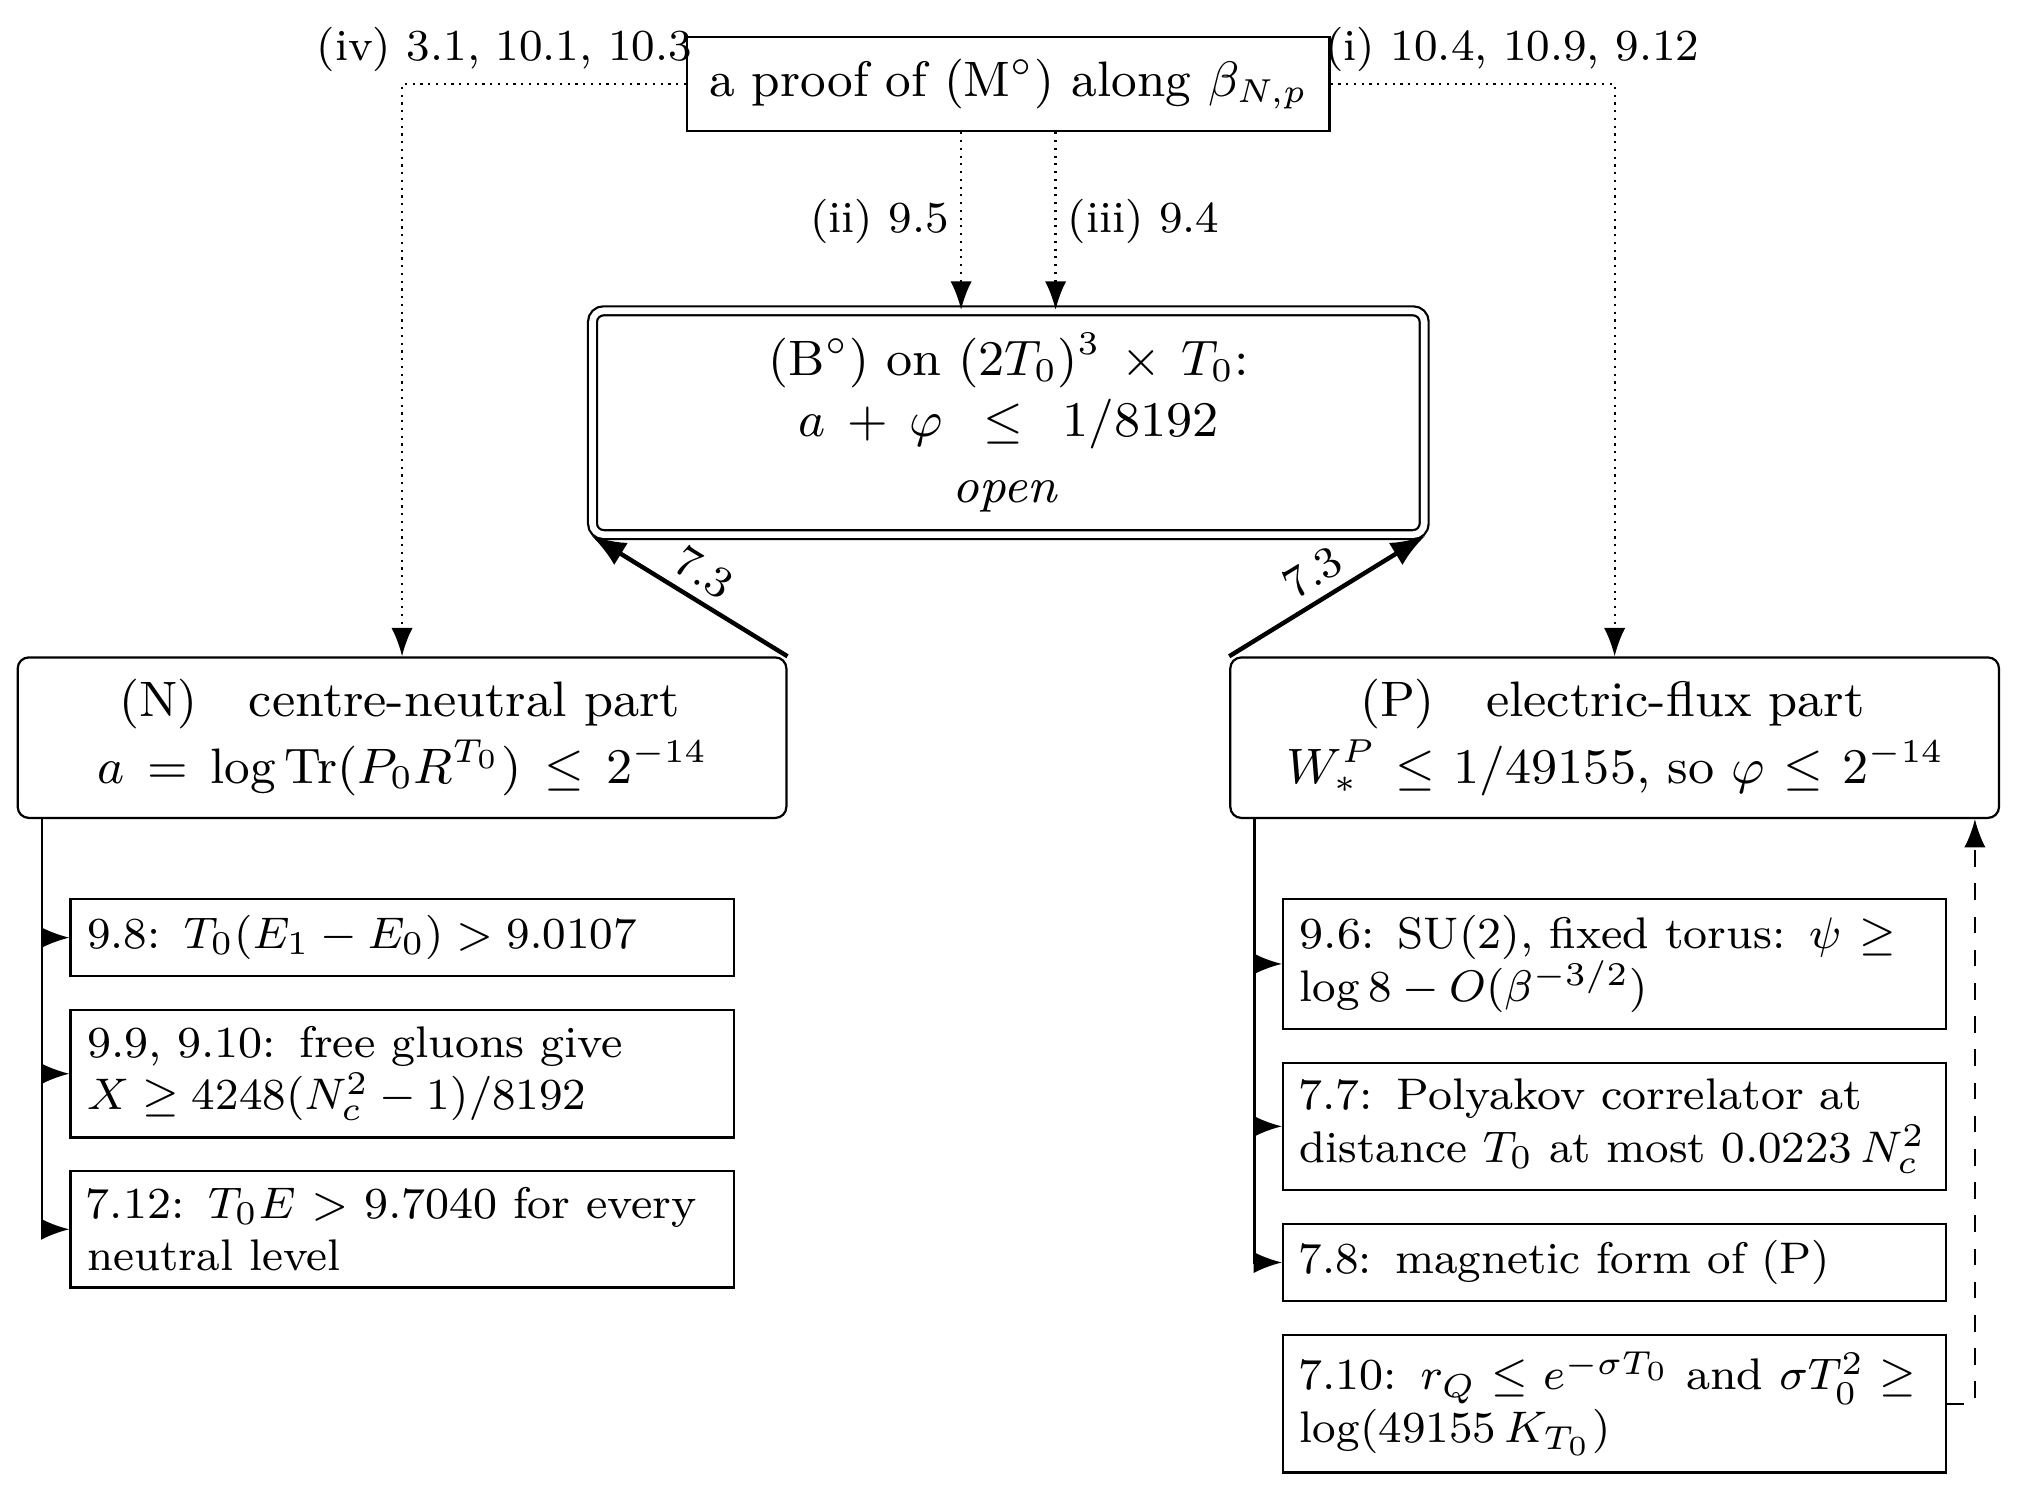
\includegraphics[width=363.0bp]{figures/fig15.png}
\caption{The wall. The open datum \Bcirc{} on $\cube{T_0}\times T_0$ (double frame) is the sum $X=a+\varphi$ of a centre-neutral part and an electric-flux part (\cref{thm:projected-split}). The conditions \hypN{} and \hypP{} imply \Bcirc{} at the same $T_0$, and \Bcirc{} implies both with tolerance $2^{-13}$ (\cref{thm:residue-split}). Below each part: proved results that bear on it, necessary conditions on the spectrum and the count of levels for the neutral part, and for the flux part the saturation on fixed tori, the Polyakov bound, the magnetic form and the conditional flux-count theorem (dashed; its hypothesis is not proved). Dotted arrows carry the requirements (i)--(iv) on a proof listed in \cref{sec:wall}.}
\label{fig:wall}
\end{figure}

\subsection*{What a proof must contain}
The proved theorems impose four requirements on any argument for \Mcirc{} along the tuning.

(i) \emph{Semisimplicity.} For compact connected $G$, every central element is a commutator if and only if $\mathfrak z(\mathfrak g)=0$, that is, if and only if $G$ is semisimple (\cref{thm:semisimplicity}(a)). On a fixed torus the cost $-\log(Z^{\mathrm{tw}}/Z)$ of a central twist is $O(\abs\Lambda\log(\abs\Lambda c))$ for $\SU(2)$ and grows linearly in $\beta$ for $\U(1)$ and for finite abelian groups (\cref{thm:semisimplicity}(b)). Abelian theories with positive-definite weights violate the datum: for Villain $\U(1)$ with $\beta\ge1$, \Bstar{} at $T_0$ forces $T_0>0.2754\,e^{\pi^2\beta/48}$, and the heat-kernel $\U(1)$ theory with $t\le1$ violates \Mcirc, \Bcirc{} and \Bstar{} at every integer $T_0\in[3,0.2\,e^{\pi^2/(32t)}]$, a range that is nonempty if and only if $t\le\pi^2/(32\log15)<0.114$ (\cref{thm:abelian}(a),(b)). For $\SU(N_c)$ the datum cannot hold together with the datum of $\SU(N_c)/\Z_{N_c}$ (\cref{thm:exclusivity}). These theorems place the non-abelian input of \Mcirc{} in the centre and in the commutator structure of $G$; that a proof must use semisimplicity is our reading of them, not a theorem.

(ii) \emph{Non-perturbative input.} On every fixed spatial torus with sides at least $3$ and every $T\ge2$, $\liminf_{\beta\to\infty}\psiT{s}{T}\ge\log2$ (\cref{thm:fixed-window}(c)), so \Mcirc{} at a fixed $T_0$ fails at all sufficiently weak couplings; for $\SU(2)$ the flux residue saturates, $\psiT{s}{T}\ge\log8-O(\beta^{-3/2})$ (\cref{prop:flux-saturation}). If the window datum holds at couplings $g_n\to0$, no infinite subfamily of these windows is uniformly controlled to any order (\cref{thm:fixed-window}(d)).

(iii) \emph{A growing base scale.} For $\SU(2)$ at $c=2\beta\ge\frac1{32}$ the gap of the cube of side $\ell$ satisfies $1-r_1\le14\ell^2\varepsilon(c)$, $\varepsilon(c)=12(\log c+5.42)/c$ (\cref{thm:fixed-torus-gap}). Hence \Bstar{} at $T_0$ with $\beta\ge3\cdot10^6$ forces $T_0^3\ge\beta/(35(\log2\beta+5.42))$, and \Bcirc{} at $T_0\ge4$ with $\betaW\ge\frac1{16}$ forces $T_0^4\varepsilon(\betaW/2)>3/32$ (\cref{cor:base-scale}(b),(c)). $T_0\ge(\beta/(35(\log2\beta+5.42)))^{1/3}$ is proved; the physically expected $T_0\ge e^{c\beta}$ is not proved.\footnote{The exponential growth is the heuristic expectation from asymptotic freedom (see the discussion after \cref{cor:base-scale}); it is used in no proof.}

(iv) \emph{A free-energy difference on one cube, and completeness of the Wilson state space.} The datum compares two partition functions, and the normalisation of the weight and $\lzero$ cancel in it (\cref{sec:psts}). The passage from one cube to all boxes and to the gap (\cref{thm:cube-control,thm:ascent}) uses only (P1) and (P2) (\cref{lem:simplicity-not-needed}): it transports the datum and does not produce it. The datum is not determined by the gauge-link observables. The product of the Wilson measure with the rings of \cref{prop:gapless-sector}(c) at $r_N=e^{-\Delta/N}$ is a simple, reflection-positive \PSTS{} with the Wilson expectations of all functions of the $G$-links, the Wilson twist ratios and the Wilson centre traces, and \Mcirc{} fails for it along every tuning (\cref{thm:hidden-sector}); the two-level systems of \cref{prop:gapless-sector}(b), whose gap in physical units tends to $0$, fail \Bcirc{} and \Mcirc{} at every $3\le T_0\le N\tzero$. A sector that does not see the centre enters only the neutral part (\cref{prop:no-residue-control}). A proof must therefore use that the transfer-matrix space of a time slice is exactly the space of square-integrable functions of the Wilson link variables of that slice.

\subsection*{What is not proved}
The four-dimensional Yang--Mills mass gap is not proved in this paper. Hypothesis \hypW, a continuum limit along the tuning whose phases are Wightman theories with a unique vacuum, is not proved. The one-cube datum \Mcirc{} is not proved at any weak coupling along the continuum tuning. For the Wilson family of \cite{openaiym} the convergence part of \hypW{} holds (\cref{lem:oai-family}); \Mcirc{} along its tuning is not proved, and the reconstruction of its non-selected phases used in \cref{thm:constructed-phases} is taken from \cite{ymgroup2026}, not proved here. Every continuum conclusion in this paper is conditional on \Mcirc{} and on \hypW, \UVB{} or the statements of \cite{openaiym}; every unconditional result is a reduction, an identity, a range at strong coupling or in two dimensions, a necessary condition, or an obstruction. The datum is proved for $\tanh\betaW<1/18$ for every compact group, for $\betaW<2/9$ for $\SU(2)$, for $\betaW<N_c^2/48$ for $\SU(N_c)$, and in two dimensions exactly; these are strong-coupling statements and do not touch the continuum tuning. \Cref{thm:San-UVB,thm:flux-count}(b) are conditional theorems. Their hypotheses, \San{} and the Hamiltonian area law with count, are not proved here; they are not weaker than \Mcirc{} in any sense proved here.

The following are open.
\begin{enumerate}[label=\textup{(\arabic*)},leftmargin=*]
\item The datum along the tuning: \Mcirc, or equivalently \Bcirc, \Hcirc{} or \Kone+\Ktwo, for the Wilson system at $\betaNp$ at some $3\le T_0\le N\tzero$, for all large $p$ and $N\ge N_0(p)$.
\item Hypothesis \hypW: in particular \UVB{} for insertions with divergent normalisation (bounded normalisation gives constant fields by \cref{thm:bounded-tokens}), $O(4)$ covariance of the limit, and its nontriviality.
\item An exponential lower bound $T_0\ge e^{c\beta}$ on the base scale; only the power bound of \cref{cor:base-scale} is proved.
\item The renormalisation-group estimates (M1) that the effective couplings of the block-spin sequence of \cite{balaban1989b} stay in $(0,\gamma]$ up to the scale $T_0$, (M2) that the localised vacuum terms satisfy the bounds (D) and (L) of \cref{prop:balaban-constant}(b) in the form (c), $A_j\le A$ and $\delta_j\le Dq^{\tau_j-1}$, with constants independent of $N$, $p$ and $s$, and (M3) that the terminal effective density satisfies \eqref{ms:eq:rational-condition} with $C_*$ replaced by $C_*-\eta(\tau)$.
\item For $\SU(2)$, the twist bound
\[
\textup{(TW)}\qquad\frac18\sum_{k\in\Z_2^3\setminus0}\Bigl(1-\frac{Z^{\mathrm{tw}}_k(s,T_0)}{Z(s,T_0)}\Bigr)\le\frac{\Vol{s}}{645(48T_0)^3}
\]
on all $s\in\Wwin_{T_0}$, uniformly along the tuning, and the monotonicity in $\beta$ of $Z^{\mathrm{tw}}/Z$ for the uniform Wilson action, which fails for general nonnegative couplings (\cref{thm:pseudoreality}).
\item The hypothesis \textup{(FS$_{\mathrm{per}}$)}$_\beta$ for the Villain $\U(1)$ theory, under which \Bcirc, \Mcirc{} and \Bstar{} fail at every $T_0\ge3$ (\cref{thm:abelian}(c)).
\item Gap monotonicity (GD$_\kappa$): $E_i(\beta_1)-E_0(\beta_1)\ge e^{-\kappa(\beta_1-\beta_0)}\bigl(E_i(\beta_0)-E_0(\beta_0)\bigr)$ for all $i\ge1$ and $\beta_1\ge\beta_0$ on the cube $\cube{T}$.
\item Explicit ranges of the datum for $\SU(N_c)$, $N_c\ge4$, beyond $\betaW<N_c^2/48$ and $\tanh\betaW<1/18$, and ranges at $\beta<0$.\footnote{For $\SU(3)$ at $\beta\ge0$ the first paper \cite[Theorem~C(i)]{bhattacharjee2026first} gives explicit ranges up to $\betaW=0.45$; this case is not listed.}
\item Non-analyticity of $\beta\mapsto\XT{\cube{T}}{T}$ at $\beta=\infty$; the only upper bound on $1-r_1$ proved here is the power law of \cref{thm:fixed-torus-gap}.
\end{enumerate}

\appendix
\section{Exact-rational constant certificates}\label{app:certificates}

This appendix lists the numerical inequalities used in the proofs, each with an exact certificate and the identifier of its machine check (\cref{app:verification}, \cref{tab:lean-julia}). An identifier L$n$ is a Lean~4 check in rational arithmetic. An identifier J$n$ is an enclosure computed with directed rounding; its endpoints are exported as rationals and checked again in Lean as rational inequalities. A dash marks an entry without a separate identifier in \cref{tab:lean-julia}; its certificate is the one written in the table. A decimal number inside an inequality denotes the rational it spells; a decimal followed by an ellipsis is a value, not a bound, and no proof uses it. The table certifies constants and nothing else.

\subsection{Enclosure rules}
Every bound on an exponential, a logarithm, $\pi$ or a root in \cref{tab:certificates} reduces to rational arithmetic through the following facts, valid for $x,y\ge0$, $0\le w\le1$ and integers $n,m\ge1$:
\begin{align}
&e^{y}-1\le\frac{y}{1-y},\qquad -\log(1-y)\le\frac{y}{1-y}\qquad(y<1);\label{eq:A-expm1}\\
&y-\frac{y^2}{2}\le\log(1+y)\le y,\qquad x-\frac{x^2}{2}\le1-e^{-x}\le x;\label{eq:A-log}\\
&S_n(y)\le e^{y}\le S_n(y)+\frac{y^{n+1}}{(n+1)!}\Bigl(1-\frac{y}{n+2}\Bigr)^{-1}\quad(y<n+2),\qquad S_n(y)=\sum_{k=0}^{n}\frac{y^k}{k!};\label{eq:A-taylor}\\
&\sum_{k=1}^{2m}\frac{(-1)^{k+1}w^k}{k}\le\log(1+w)\le\sum_{k=1}^{2m+1}\frac{(-1)^{k+1}w^k}{k};\qquad 3.141592<\pi<3.141593.\label{eq:A-alt}
\end{align}
\emph{Proofs.} $e^{-y}\ge1-y$ gives $e^{y}\le(1-y)^{-1}$, and $-\log(1-y)=\log(1+\frac{y}{1-y})\le\frac{y}{1-y}$ by \eqref{eq:A-log}. The four differences in \eqref{eq:A-log}, $\log(1+y)-y+\frac{y^2}2$, $y-\log(1+y)$, $1-e^{-x}-x+\frac{x^2}2$ and $x-1+e^{-x}$, vanish at $0$ and have the nonnegative derivatives $\frac{y^2}{1+y}$, $\frac{y}{1+y}$, $e^{-x}-1+x$, $1-e^{-x}$. In \eqref{eq:A-taylor}, $k!\ge(n+1)!\,(n+2)^{k-n-1}$ for $k>n$ bounds the tail by a geometric series of ratio $y/(n+2)$. In \eqref{eq:A-alt} the terms $w^k/k$ decrease to $0$, so consecutive partial sums bracket the alternating series; the same argument applied to Machin's formula $\pi=16\arctan\frac15-4\arctan\frac1{239}$ gives the enclosure of $\pi$.

\emph{Use.} A lower bound $\log a>b$ is certified as $e^{b}<a$ by the upper half of \eqref{eq:A-taylor}, an upper bound $\log a<b$ as $e^{b}>a$ by the lower half; for $b>1$ one writes $e^{b}=(e^{b/2^k})^{2^k}$ with $b/2^k\le1$. Bounds on $e^{-x}$ are reciprocals of bounds on $e^{x}$, roots are compared through powers ($\sqrt a<b\iff a<b^2$ for $b>0$), and $\pi$ enters only through \eqref{eq:A-alt}. Every upper bound on $e^{\pi}$ or $e^{2\pi}$ in the table uses $\pi<3.141593$.

\subsection{Three recurring computations}
\emph{The ascent map.} \Cref{thm:ascent,thm:zero-one,thm:upward-closed} use $f(x)=(e^{64x}-1)^2$, and \eqref{eq:A-expm1} gives
\begin{equation}\label{eq:A-majorant}
f(x)\le g(x):=\Bigl(\frac{64x}{1-64x}\Bigr)^{2}\qquad\bigl(0\le x<\tfrac1{64}\bigr).
\end{equation}
The quotient $f(x)/x=\frac{e^{64x}-1}{x}(e^{64x}-1)$ is a product of two positive increasing functions and tends to $0$ as $x\downarrow0$. Hence $f(x)=x$ has exactly one positive root $x_c$, with $f(x)<x$ on $(0,x_c)$ and $f(x)>x$ on $(x_c,\infty)$, and a bracket of $x_c$ needs only two values of $f$. The majorant iterates $x_{i+1}=g(x_i)$, $x_0=\xconstinl$, computed in exact rational arithmetic and rounded upward to the grid $10^{-40}$ after each step, satisfy
\begin{equation}\label{eq:A-iterates}
\begin{aligned}
&x_1=\tfrac1{16129}\le6.2001\cdot10^{-5},&&x_2\le1.5871\cdot10^{-5},\\
&x_3\le1.03381\cdot10^{-6},&&x_4\le4.3783\cdot10^{-9}.
\end{aligned}
\end{equation}
Since $f\le g$ and both maps are increasing, the exact iterates of $f$ lie below those of $g$; every upper bound stated through the exact iterates remains true with \eqref{eq:A-iterates}.

\emph{The theta series of \cref{thm:two-dim}.} There $\psi_{\mathrm{cont}}(x)=2\log\Theta(x)-\log\Theta(2x)$ with $\Theta(x)=\sum_{n\ge1}e^{-(n^2-1)x/8}$. Since $(n^2-1)/8\ge(n-1)/2$ for $n\ge3$,
\begin{equation}\label{eq:A-theta}
1+e^{-3x/8}\le\Theta(x)\le1+e^{-3x/8}+\frac{e^{-x}}{1-e^{-x/2}}\qquad(x>0),
\end{equation}
and the bracket of $\kappa_c$ follows from \eqref{eq:A-theta}, \eqref{eq:A-taylor} and \eqref{eq:A-log} at $x=23.872$ and $x=23.874$.

\emph{The certified triples of \cref{cor:certified-triples}.} For a row $(\betaW,z,T_*)$ of \cref{tab:certified-triples} put $\kappa(z)=\max\{12+4z+2z^2,\,6+12z\}$, $\theta=c\,\kappa(z)$ with $c=\tanh\betaW$ (any compact group; bounded above through an upper bound on $e^{2\betaW}$ in $\tanh\betaW=\frac{e^{2\betaW}-1}{e^{2\betaW}+1}$) or $c=\betaW/4$ ($\SU(2)$), and $L=(1-\theta)/(96\cdot161\cdot48^3\betaW z)$. The check verifies in rational arithmetic that $\theta<1$, $T_*$ is even, $(1+2/T_*)^2\le z$ and $(T_*+1)^4\le Lz^{T_*}$. The last two give the datum for every $T\ge T_*$: $T^4z^{-2\lfloor T/2\rfloor}\le L$ at $T\in\{T_*,T_*+1\}$, and $T^4z^{-2\lfloor T/2\rfloor}$ does not increase under $T\mapsto T+2$.

Numbers displayed in the body with the sign $\approx$ are numerical illustrations and enter no proof: $\tau_c\sqrt{\sigma_{\mathrm{ph}}}\approx2.1157$ in \cref{thm:two-dim}, $q_{\Gharm}\approx0.985(N^2-1)$ in \cref{thm:universal-step}, and the Julia values listed as sanity checks in \cref{app:verification}. The finite identities of \cref{prop:sector-zero} (a character identity on $(\Z/N)^3$, check L10) and of \cref{lem:lemma-W} (polynomial identities in quaternion coordinates, check L11) are exact but are not numerical inequalities; they are treated in \cref{app:verification,app:lemma-W}. None of the certificates above bears on the datum \Mcirc{} along the continuum tuning, on hypothesis \hypW, or on the mass gap.

\Cref{tab:certificates} is ordered by the section in which each inequality is used; the first column gives the results whose proofs use it, and \emph{Cert.}\ introduces the certificate.

{\footnotesize\sloppy\setlength{\tabcolsep}{3pt}\renewcommand{\arraystretch}{1.05}
\begin{longtable}{@{}p{0.11\textwidth}p{0.80\textwidth}p{0.055\textwidth}@{}}
\caption{Exact certificates for the numerical inequalities used in the proofs.}\label{tab:certificates}\\
\toprule
Item & Inequality or identity, and certificate & Check\\
\midrule
\endfirsthead
\caption[]{(continued)}\\
\toprule
Item & Inequality or identity, and certificate & Check\\
\midrule
\endhead
\bottomrule
\endfoot
\labelcref{lem:purity-conversion}, \labelcref{thm:ascent} & $2x-3x^2\ge\dconstinl$ at $x=\xconstinl$. \emph{Cert.}\ $2x-3x^2=\frac{16381}{67108864}$ and $\frac{16381}{67108864}-\frac1{4097}=\frac{4093}{274945015808}$. & L1\\
\labelcref{cor:window-datum} & $40\cdot96^3=35\,389\,440$; $161\cdot48^3=17\,805\,312$; $2x-3x^2\ge\frac1{17\,805\,313}$ at $x=\frac1{322\cdot48^3}$. \emph{Cert.}\ With $a=161\cdot48^3$: $2x=\frac1a$ and $\frac1a-\frac1{a+1}=\frac1{a(a+1)}\ge\frac3{4a^2}=3x^2$, because $a\ge3$. & L2\\
\labelcref{thm:ascent} & $v_i:=e^{64x_i}-1\le\theta^{-1}u^{2^i}/64$ for the exact iterates $x_{i+1}=v_i^2$, $x_0=\xconstinl$, where $\theta=\frac{127}{126}$, $u=\frac{32}{63}$. \emph{Cert.}\ $\theta^{-1}u/64=\frac1{127}\ge e^{1/128}-1$ by \eqref{eq:A-expm1}; inductively $64v_i^2\le\frac{64}{127^2}<\frac1{252}$, so $v_{i+1}\le\frac{252}{251}\,64v_i^2$ by \eqref{eq:A-expm1}, and $\frac{252}{251}\le\theta$. & J2\\
\labelcref{thm:ascent}, \labelcref{thm:main} & $\log\frac{63}{32}>0.67725>0.677$; $u^8<\frac1{128}$. \emph{Cert.}\ $e^{0.67725}\le S_8(0.67725)+10^{-7}<1.96846<\frac{63}{32}=1.96875$ by \eqref{eq:A-taylor}; $u^8=2^{40}/63^8<0.00444$. & J2\\
\labelcref{thm:ascent} & $x_4<\frac1{40\cdot96^3}$, so \Bcirc{} at $T_0$ gives \Bstar{} at $16T_0$. \emph{Cert.}\ \eqref{eq:A-iterates}: $x_4\le4.3783\cdot10^{-9}<2.825\cdot10^{-8}<\frac1{35\,389\,440}$. & L14, L2\\
\labelcref{thm:dyadic-gap} & $10(e^{6.4}-1)<e^{8.71}$, so $\delta T_0\ge8.71$ suffices. \emph{Cert.}\ $e^{6.4}<601.85$ and $e^{8.71}>6063$ by \eqref{eq:A-taylor}; $10\cdot600.85=6008.5$. & --\\
\labelcref{thm:zero-one} & $x_c\in(\frac1{4160},\frac1{4159})$; $e^{1/4159}<2$. \emph{Cert.}\ Monotonicity of $f(x)/x$; $4160\,f(\frac1{4160})<0.99991$ by the upper and $4159\,f(\frac1{4159})>1.00014$ by the lower half of \eqref{eq:A-taylor}; $e^{1/4159}-1\le\frac1{4158}<1$ by \eqref{eq:A-expm1}. & J1\\
\labelcref{thm:upward-closed} & $64x_1<3.9681\cdot10^{-3}$, $64x_2<1.0158\cdot10^{-3}$, $64x_3\le6.6164\cdot10^{-5}<\xconstinl$; $2\cdot\xconstinl=\frac1{4096}$. \emph{Cert.}\ \eqref{eq:A-iterates}, with $64x_1=\frac{64}{16129}$; as $64x_1,64x_2>\xconstinl$, the bound starts at the third scale; the inequality (E3) of \cref{lem:E1-E3} gives $\psi\le2X\le\frac1{4096}$. & L14\\
\labelcref{thm:upward-closed} & At $\rho=\frac1{1\,769\,473}$: $216\log(1+\rho)<\xconstinl$ and $432\log(1+\rho)-216\log(1+\rho^2)>\dconstinl$, so the converse implication fails. \emph{Cert.}\ $216\cdot8192=1\,769\,472$, hence $216\log(1+\rho)\le216\rho<\frac1{8192}$; by \eqref{eq:A-log} the second quantity is $\ge432\rho(1-\rho)$, and with $a=1\,769\,473$: $432\cdot4097\,(a-1)-a^2=430a-431>0$. & J11, L14\\
\midrule
\labelcref{prop:hypercube-converse} & $\frac{16}{8191^2}+\frac8{511^2}+\frac4{255^2}+\frac2{127^2}<2.17\cdot10^{-4}<\dconstinl$. \emph{Cert.}\ The terms come from $e^{k/8192}-1\le\frac{k}{8192-k}$, $k=1,16,32,64$ \eqref{eq:A-expm1}; the sum is $<2.1640\cdot10^{-4}$, and $\frac1{4097}>2.4408\cdot10^{-4}$. & L4, J12\\
\labelcref{thm:casimir-criterion} & $\frac{11}{10^5}+\frac1{299^2}<\xconstinl$; $\frac1{127^2}+\frac2{255^2}+\frac4{511^2}<1.081\cdot10^{-4}<\frac{11}{10^5}$; $8191^{-2}\le\frac1{300}$. \emph{Cert.}\ $e^{1/300}-1\le\frac1{299}$ by \eqref{eq:A-expm1}; $\frac{11}{10^5}+\frac1{299^2}<1.21186\cdot10^{-4}<1.22070\cdot10^{-4}<\frac1{8192}$; the second sum is $<1.08077\cdot10^{-4}$. & --\\
\cref{fn:kogut-susskind} & $9.0108<-\log(e^{1/8192}-1)<13\log2<9.011$. \emph{Cert.}\ With $h=2^{-13}$, $e^{h}-1>h$ gives the upper bound; $e^{h}-1\le h(1+0.5001h)$ by \eqref{eq:A-taylor} ($n=2$) and $13\log2>9.0109$ give $-\log(e^{h}-1)\ge13\log2-0.5001h>9.0108$. & J3\\
\labelcref{thm:residue-split} & $\frac3{49155}=\frac1{16385}$; $\frac{1/16385}{1-1/16385}=2^{-14}$; $-\log(1-\frac1{16385})\le2^{-14}$; $2\cdot2^{-14}=2^{-13}$; $1-e^{-2^{-13}}\le2^{-13}$. \emph{Cert.}\ $49155=3\cdot16385$, $16385=2^{14}+1$; \eqref{eq:A-expm1}, \eqref{eq:A-log}. & L3\\
\labelcref{prop:window-split} & $2\cdot\frac{161}{645}\cdot\frac{645}{644}=\frac12$; $1-x-x^2\ge1-2x+2x^2$ for $0\le x\le\frac13$, used at $x\le\frac1{161}$. \emph{Cert.}\ $644=4\cdot161$; the inequality is $x\ge3x^2$. & L8\\
\labelcref{prop:polyakov-bound} & $\frac2{\sqrt{8192}}+\frac1{8192}<0.0223$. \emph{Cert.}\ $\frac2{\sqrt{8192}}=\frac{\sqrt2}{64}$ and $\bigl(\frac{\sqrt2}{64}\bigr)^2=\frac1{2048}<4.8829\cdot10^{-4}<4.9186\cdot10^{-4}<\bigl(0.0223-\frac1{8192}\bigr)^2$. & --\\
\cref{fn:area-law}, \labelcref{thm:magnetic-P}, \labelcref{thm:flux-count} & $e^{10.80}<49155<e^{10.81}$, so $\frac12\log49155\in(5.40,5.41)$; $2\cdot49155^{-1/4}\in(0.1342,0.1344)$; $\frac2{49153}<4.07\cdot10^{-5}$, $\frac3{49152}=\frac1{16384}$; $1-t\ge e^{-t/(1-t)}$ for $0\le t<1$; $\frac{49155}{8192}\in(6.00036,6.00037)$. \emph{Cert.}\ $e^{10.80}<49020.81$ and $e^{10.81}>49513.4$ by \eqref{eq:A-taylor}; $(2/0.1344)^4<49037<49155<49329<(2/0.1342)^4$; the fourth claim is \eqref{eq:A-expm1}; $\frac{49155}{8192}=6+\frac3{8192}$. & J10\\
\labelcref{cor:neutral-threshold} & $9.70403<-\log(e^{2^{-14}}-1)<9.70404<14\log2$. \emph{Cert.}\ With $h=2^{-14}$, $-\log(e^h-1)=14\log2-\log\frac{e^h-1}h$, where $\frac h2-\frac{h^2}8\le\log\frac{e^h-1}h\le\frac h2+\frac{h^2}5$ by \eqref{eq:A-log}, \eqref{eq:A-taylor}, and $14\log2\in(9.70406052,9.70406053)$. & J3\\
\midrule
\labelcref{thm:strong-coupling} & $\tanh\betaW<\frac1{18}\iff\betaW<\operatorname{artanh}\frac1{18}\in(0.0556128,0.0556129)$; for $\SU(2)$, $18\cdot\frac{\betaW}4<1\iff\betaW<\frac29$. \emph{Cert.}\ $\operatorname{artanh}\frac1{18}=\frac12\log(1+\frac2{17})$, bracketed by \eqref{eq:A-alt}. & J8\\
\labelcref{cor:certified-triples} & The four conditions above on each row of \cref{tab:certified-triples}. \emph{Cert.}\ $\theta\le0.522$, $0.820$, $0.840$, $0.960$, $0.99917$, $0.99890$ (any $G$) and $\theta=0.96$, $0.975$, $0.99$, $0.9999$ ($\SU(2)$); in every row the last condition fails with $T_*-2$ in place of $T_*$, that is, the bound $T^4z^{-2\lfloor T/2\rfloor}\le L$ fails at $T=T_*-1$; e.g.\ for $(\betaW,z)=(\frac1{1000},15)$ it holds at $T=10$ and fails at $T=11$. & J8\\
\labelcref{cor:certified-triples} & $u=32(e^{\eta_0}-1)^2/\eta_0\le0.478892<0.479$ for $\eta_0=\frac{128}{27}F(\frac1{161})\le0.014746$, $F$ the inverse of $x\mapsto-\log[e^{-2x}+(1-e^{-x})^2]$; $(4095\cdot32)^{-2}<5.9\cdot10^{-11}$. \emph{Cert.}\ With $t=1-e^{-x}$ the bracket is $1-2t+2t^2$, which decreases in $t\in[0,\frac12]$, that is, in $x\in[0,\log2]$; so $F$ is increasing. At $x_+=0.00311048$: $t\ge t_-:=1-1/S_6(x_+)$ by \eqref{eq:A-taylor}, and $(1-2t_-+2t_-^2)\,e^{1/161}<1-7\cdot10^{-8}$ by the upper half of \eqref{eq:A-taylor}; hence $F(\frac1{161})<x_+$ and $\eta_0<\frac{128}{27}x_+<0.014746$. As $(e^{\eta}-1)/\eta$ and $e^\eta-1$ increase in $\eta$, $u<32\cdot0.01485526^2/0.014746<0.478891$, using $e^{0.014746}-1<0.01485526$ from \eqref{eq:A-taylor} ($n=3$). Finally $(4095\cdot32)^{-2}=5.8236\ldots\cdot10^{-11}$; $e^x-1\le\frac{4096}{4095}x$ for $0\le x\le\frac1{4096}$ by \eqref{eq:A-expm1}. & --\\
\labelcref{thm:large-N} & $K_0=239\cdot161\cdot48^3=4\,255\,469\,568$; $48\pi\sqrt{5/2}<239$; $4\pi\sqrt{5/2}<19.87$; $4K_0<1.71\cdot10^{10}$. \emph{Cert.}\ $\pi<3.1416$ and $\bigl(\frac{238.44}{48\cdot3.1416}\bigr)^2>2.5$, with $238.44=12\cdot19.87$; $4K_0=17\,021\,878\,272$; $\alpha=\frac{36\beta}{1-12\beta}=\frac1{13},\frac15,\frac37,\frac9{13}$ at $\beta=\frac1{480},\frac1{192},\frac1{96},\frac1{64}$. & L6\\
\labelcref{thm:large-N} & Least $T_*$ with $K_0N_c^2\beta T^4\alpha^h\le h+1$, $h=\lfloor\frac{T-3}2\rfloor$, for every $T\ge T_*$: $25,41,81,199$ ($N_c=2$); $27,43,83,205$ ($N_c=3$); $29,45,89,219$ ($N_c=10$); $47,77,147,351$ ($N_c=10^6$). \emph{Cert.}\ Exact evaluation for $5\le T<6000$; for $T\ge6000$ the explicit $T_*(\beta,N_c)$ of \cref{thm:large-N} applies, its value being below $601$ in all sixteen cases. & J9\\
\labelcref{thm:two-dim} & $\frac{2T_0}{161\cdot48T_0}=\frac1{3864}=\frac2{7728}$; $e^9>7729$; $\log7729<8.953$; $\log7700>8.948$; $\frac2{7700}-\frac2{7700^2}>\frac1{3864}$; $\frac43\cdot8.953<11.9374$, $\frac43\cdot8.948>11.9306$. \emph{Cert.}\ \eqref{eq:A-taylor}; the fifth claim is $15398\cdot3864=59\,497\,872>7700^2=59\,290\,000$; $\frac43\cdot8.953=11.93733\ldots$, $\frac43\cdot8.948=11.93066\ldots$. & J7\\
\labelcref{thm:two-dim} & $\kappa_c\in(11.936,11.937)$, where $\psi_{\mathrm{cont}}(2\kappa_c)=\frac1{3864}$. \emph{Cert.}\ $\psi_{\mathrm{cont}}(23.872)>2.5892\cdot10^{-4}>\frac1{3864}>2.5873\cdot10^{-4}>\psi_{\mathrm{cont}}(23.874)$, from \eqref{eq:A-theta}. & J7\\
\midrule
\labelcref{thm:fixed-torus-gap}, \labelcref{cor:base-scale} & $\frac12+\frac83+\frac32=\frac{14}3$; $3\cdot\frac{14}3=14$; $\frac{9.6}{56\cdot6}=\frac1{35}$. \emph{Cert.}\ Exact. & L7\\
\labelcref{thm:SUN-gap} & $(1-\frac{0.58^2}6)^2>0.94^2$; $\frac1{c_2}<16.05$ for $c_2=\frac{0.94^3\cdot4\pi/3}{4\sqrt2\,\pi^2}=\frac{0.94^3}{3\sqrt2\,\pi}$; $1+\frac23\log\frac1{c_2}+\log8<4.931$, so $\varepsilon_2(b)\le\frac{12}b(\log b+4.931)$. \emph{Cert.}\ $6-0.58^2=5.6636>5.64=6\cdot0.94$; $\sqrt2<1.41422$, $\pi<3.1416$ give $\frac1{c_2}<16.0475$; $\frac23\log16.05<1.8505$, $\log8<2.0795$. & --\\
\labelcref{cor:base-scale} & $D=e^{1/(5\cdot96^3)}-1\le2.2606\cdot10^{-7}$, $\log\frac1D\ge15.3024$; $1-e^{-1}\ge0.632$; $0.632\cdot15.30\ge9.6$; $\varepsilon_0=\frac{0.632^3}{56\cdot9.6^2}>4.8912\cdot10^{-5}>\varepsilon(6\cdot10^6)$ for $\varepsilon(b)=\frac{12}b(\log b+5.42)$; $\frac{9.6}{0.632}<15.19$. \emph{Cert.}\ $5\cdot96^3=4\,423\,680$ and \eqref{eq:A-expm1}; $\varepsilon$ decreases for $b>e^{-4.42}$; $\varepsilon(6\cdot10^6)<4.2055\cdot10^{-5}$. & J5, L7\\
\labelcref{cor:base-scale} & One-cube $\SU(2)$ form and crossing coupling: $0.632\cdot9.0107>5.69$; $\frac{64\cdot3}{320}<5.69$; $\frac{64\cdot3}{32\cdot16}=0.375<0.632$; $e^{10.39}<2^{15}$, $e^{3.27}>26.22$; $\frac8{17\,805\,312}<\dconstinl$; $e^9<8191$. \emph{Cert.}\ \eqref{eq:A-taylor}: $e^{10.39}<32533$, $e^{3.27}>26.31$, $e^9<8103.1$; $0.632\cdot9.0107=5.6947\ldots$. & --\\
\labelcref{prop:spectral-conditions} & $13\log2\in(9.0109,9.011)$; $13\log2-2^{-13}>9.0107$; $e^{2^{-13}}-1\le2^{-13}(1+2^{-13})<\frac1{8191}$; $2^{-12}(1+2^{-13})<\frac1{4095}$; $8192e^{-9.01}>1$. \emph{Cert.}\ $e^{9.0109}<8191.9<8192<8192.7<e^{9.011}$; $e^{h}-1\le h+h^2$ for $0\le h\le1$; $8193\cdot8191<8192^2$; $\frac1{4095}-\frac{8193}{4096\cdot8192}=\frac{4097}{4095\cdot4096\cdot8192}$; $e^{9.01}<8184.6$. & J3\\
\labelcref{prop:no-stefan-boltzmann} & $12e^{-2\pi}>0.0223>2^{-13}$; $\frac{9.01}{2\pi}>1.43$; the $12$ two-gluon singlet states. \emph{Cert.}\ $e^{2\pi}<535.5$, so $12e^{-2\pi}>0.02240$; $1.43\cdot6.283186<8.986$; the count is a finite enumeration. & J4, L13\\
\labelcref{thm:free-gluon} & $e^{-\pi}>0.04321$, $12e^{-\pi}>0.518$; $12\cdot8192\,e^{-\pi}>4248$; $24\cdot4097\,e^{-\pi}>4249$; $-\log(e^{1/8192}-1)>9.0108$; $e^{9.0108-\pi}>353$; $\log(2+\sqrt3)\ge0.76\sqrt3$; with $b=\frac{1.52}{\sqrt3}$, $\frac{2}{1-e^{-1.52}}\bigl[\bigl(\frac{1+e^{-b}}{1-e^{-b}}\bigr)^3-1\bigr]\le33.88<34$. \emph{Cert.}\ $e^{\pi}<e^{3.141593}<23.1408<\frac{98304}{4248}=23.1412\ldots$ (margin $5\cdot10^{-4}$); $\frac{98328}{23.1408}>4249.1$; row of \cref{fn:kogut-susskind}; $e^{9.0108}>8191$; $0.76\sqrt3<1.31637$ and $e^{1.31637}<3.72986<2+\sqrt3$; $\sqrt3<1.7320509$ gives $b>0.87757$, and $e^{1.52}>4.5722$, $e^{0.87757}>2.405$ by \eqref{eq:A-taylor}; the expression increases in $e^{-1.52}$ and in $e^{-b}$, so it is $<\frac{2}{1-1/4.5722}\bigl[\bigl(\frac{1+1/2.405}{1-1/2.405}\bigr)^3-1\bigr]<33.878$. & J4, J11\\
\labelcref{thm:free-gluon} & $12\log2>8.317>2\pi$; $f(k)=-\log(1-e^{-2\pi/k})\bigl(\frac{2k}{k-1}\bigr)^6\ge81$ for $k>1$, so the shortfall is $\ge12\cdot81=972$. \emph{Cert.}\ $12\log2=4\log8$ and $e^{2.0794}<7.9997<8$ by \eqref{eq:A-taylor}, so $12\log2>8.3176$; $2\pi<6.283186$; for $f$: if $k\le1.25$, $(\frac{2k}{k-1})^6\ge10^6$ and the logarithm is $\ge e^{-2\pi}>1.86\cdot10^{-3}$; for $k\ge20$ the power is $\ge64$ and the logarithm, increasing in $k$, exceeds $1.31$, with $64\cdot1.31>83.8$; on $[1.25,20]$ a grid of step $\frac1{500}$ with the two factors bounded at opposite ends. & J4\\
\labelcref{thm:pair} & $\log(1+e^{-2\pi})>\frac{15}{8192}$. \emph{Cert.}\ $y=e^{-2\pi}>\frac1{535.5}$; by \eqref{eq:A-log}, $\log(1+y)\ge y-\frac{y^2}2>1.8656\cdot10^{-3}>1.8311\cdot10^{-3}>\frac{15}{8192}$. & J4\\
\labelcref{thm:exclusivity} & $q_N=\frac{4N^3-6N+3}{N^3}\ge q_2=\frac{23}8$ for $N\ge2$; $\bigl(\frac{23}8-\frac{4097}{4096}\bigr)/\frac98>1.666$; $\bigl(\frac{23}8-\frac{4097}{4096}\bigr)/4>0.468$; $\frac{23}8-\frac98\cdot\frac1{4096}>2.874$. \emph{Cert.}\ $q_N=4-6N^{-2}+3N^{-3}$ and $\frac{d}{dN}q_N=\frac{12N-9}{N^4}>0$. & L5\\
\labelcref{prop:finite-volume-gap} & $\theta_d=\frac1{161\cdot24^{d-1}}=\frac1{2\,225\,664},\frac1{92\,736},\frac1{3864}$ ($d=4,3,2$); $\sqrt{1-2\theta}\ge1-\theta-\theta^2$ for $0\le\theta\le\sqrt2-1$; for $q\le\frac{\theta+\theta^2}{2-\theta-\theta^2}$, $\log\frac1q\ge15.3087$, $12.1306$, $8.9522$, whence $\delta\ell\ge30.6$, $24.2$, $17.9$; $\frac{13}8\cdot17\,805\,312\,e^{-\pi\sqrt3}\ge125\,381>1.25\cdot10^5$; $370\,944\,e^{-\pi\sqrt2}\ge4363>4.3\cdot10^3$. \emph{Cert.}\ $(1-\theta-\theta^2)^2=1-2\theta-\theta^2(1-2\theta-\theta^2)$; \eqref{eq:A-taylor}; $370\,944=161\cdot48^2$; $\sqrt3<1.7320509$, $\sqrt2<1.4142136$. & J7\\
\midrule
\labelcref{thm:no-convexity} & $\frac\pi2(16+0.72\log4)<26.71$; $\frac\pi2\cdot1.44<2.27$; $-\frac{3.870-6.5\cdot10^{-8}}{2(1+\rho)}\le-1.89$ for $0\le\rho\le21\phi e^{-46}$; $\frac{(2\pi-0.2)^2}8\ge4.61$; $G(\phi)/\phi\le-3.870$ on $(0,\frac1{10}]$ for the function $G$ of the proof. \emph{Cert.}\ $\log4<1.3863$; $\frac{3.870-6.5\cdot10^{-8}}2>1.93499$, and $1.93499/(1+\rho)\ge1.89$ for $\rho\le0.0238$, while $21\phi e^{-46}<10^{-19}$; $\pi>3.141592$. For $G$: $G(\phi)=\sum_{n\ge1}g_n\phi^n$ with $g_1,\dots,g_6=-4,\frac54,\frac{79}{192},-\frac{673}{1536},\frac{21473}{245760},\frac{9643}{393216}$ (exact); the function $M$ obtained from the formula for $G$ by replacing $\cos,\sin,e^{-x}$ by $\cosh,\sinh,e^{x}$ and every minus sign by a plus sign has coefficients $m_n\ge\abs{g_n}$, and $\sum_nm_n=M(1)<100.39$ by \eqref{eq:A-taylor}; so for $0<\phi\le\frac1{10}$, $G(\phi)/\phi\le-4+\sum_{n=2}^6\abs{g_n}10^{1-n}+10^{-6}M(1)<-3.87033$. & --\\
\labelcref{thm:BE-line-field} & $c_+^*\ge13.9723$, $c_-^*\ge13.9471$; $9+\sqrt{17}>\frac{38}3$; $\frac{14.5}{13.9723}<1.0378$ ($\beta\ge0$); $\frac{14.5}{13.9471}<1.0397$ ($\beta<0$). \emph{Cert.}\ $c_+(\Lambda_m)\ge R_+-\frac{56}m$ and $c_-(\Lambda_m)\ge R_--\frac{59}m$, where $R_\pm$ are the exact rational Rayleigh quotients of the two test fields listed at the end of this appendix: $R_+>13.97233$, $R_->13.94719$; the boundary losses come from $\max_e\abs{X_e}^2/\sum_e\abs{X_e}^2=\frac{525483}{16378696},\frac{543521}{16161106}$, with $1728\cdot\frac{525483}{16378696}<55.45$ and $1728\cdot\frac{543521}{16161106}<58.12$; let $m\to\infty$. $\sqrt{17}>\frac{11}3$ as $17>\frac{121}9$. & --\\
\labelcref{thm:BE-orbit} & $\frac{135\sqrt3}8<30$; $12\sqrt3<21$. \emph{Cert.}\ $135^2\cdot3=54\,675<240^2$; $432<441$. & --\\
\labelcref{thm:abelian} & $De^{1/4}\le2.903\cdot10^{-7}$; $\log(1.5-1.4515\cdot10^{-7})\ge0.405465$; $\frac{0.405465}{70.4}>0.2754^4$. \emph{Cert.}\ $D$ as for \cref{cor:base-scale}; $\frac{0.405465}{70.4}>0.0057594>0.0057525>0.2754^4$; with $d=1.4515\cdot10^{-7}$, \eqref{eq:A-expm1} gives $\log(1.5-d)\ge\log1.5-\frac d{1.5-d}$ and $\frac d{1.5-d}<9.677\cdot10^{-8}$, while \eqref{eq:A-alt} with $w=\frac12$, $m=11$ gives $\log1.5>0.40546510$; the difference exceeds $0.405465$ by more than $3\cdot10^{-9}$. & J5\\
\labelcref{thm:abelian} & Heat-kernel $\U(1)$: $8e^{-\pi}-0.3072>0.0385>\dconstinl>\frac8{161\cdot48^3}$, where $0.3072=192\cdot0.2^4$; $\frac{16}{40\cdot96^3}<4.6\cdot10^{-7}$; $0.2\,e^{\pi^2/(32t)}\ge3\iff t\le\frac{\pi^2}{32\log15}$, and $\frac{\pi^2}{32\log15}<0.114$; $\vartheta(c)-1\le3e^{-c}$ for $c\ge\frac13\log3$. \emph{Cert.}\ $8e^{-\pi}>\frac8{23.1408}>0.345709$ and $0.345709-0.3072=0.038509$; $\pi^2<9.8697$ and $e^{2.708}<14.9993$ by \eqref{eq:A-taylor}, so $\frac{\pi^2}{32\log15}<\frac{9.8697}{86.656}<0.11390$; $\frac8{17805312}<4.5\cdot10^{-7}$; $\vartheta(c)=\sum_{m\in\Z}e^{-cm^2}$ and $m^2\ge3m-2$ give $\vartheta(c)-1\le\frac{2e^{-c}}{1-e^{-3c}}$. & --\\
\labelcref{thm:pseudoreality} & $\int\prod_{p\in S}\Tr U_p=-2^{-27}=-\frac1{134\,217\,728}$; for $S'$ the value is $-2^{-43}$; $(F,E,\hat V,\chi)=(28,56,29,1)$ and $(42,84,41,-1)$. \emph{Cert.}\ Finite $\SU(2)$ Haar moment computations (\cref{app:surfaces}); $\chi=\hat V-E+F$. & L12\\
\labelcref{thm:finite-rank-obstruction} & $12\cdot3\cdot161\cdot144^3=17\,306\,763\,264$; Lipschitz radius $\frac1{72\cdot161\cdot144^3}=\frac1{34\,613\,526\,528}<2.8891\cdot10^{-11}$; $138^3=2\,628\,072$ window tori; thermal quantity $\Tr R^T-1\le9.5\cdot10^{-4}$ at the seven certified couplings. \emph{Cert.}\ The counts are exact. With the plaquette weight $e^{(\beta/2)\tr U_p}$ one has $\Tr R^T-1=\sum_{n\ge1}\alpha_n^{LT}$, $\alpha_n=I_{n+1}(\beta)/I_1(\beta)$; on $L=T=\lceil\sqrt{4.6\beta}\rceil$ the outward-rounded enclosures give the upper values $1.5341\cdot10^{-6}$, $5.7200\cdot10^{-5}$, $3.2022\cdot10^{-4}$, $6.4075\cdot10^{-4}$, $8.7522\cdot10^{-4}$, $8.7974\cdot10^{-4}$, $9.4626\cdot10^{-4}$ at $(\beta,L)=(2,4)$, $(8,7)$, $(32,13)$, $(128,25)$, $(512,49)$, $(2048,98)$, $(8192,195)$, the ratios computed by backward recurrence and the tail $n\ge N\ge\beta$ bounded by $I_{n+2}/I_{n+1}\le\beta/(2(n+2))\le\frac12$. & --\\
\labelcref{prop:trivialising-maps} & $\delta=\frac{72\varepsilon}{1-27\varepsilon}\Rightarrow\frac{1-\delta}{2\delta}=\frac{1-99\varepsilon}{144\varepsilon}$; $144\cdot12=1728$; for $c\ge\frac1{32}$, $\varepsilon_8(c)=\frac{12(\log c+5.42)}c<\frac1{99}$ holds for $c\ge18085$ and fails for $c\le18084$. \emph{Cert.}\ $1-\delta=\frac{1-99\varepsilon}{1-27\varepsilon}$; $c-1188(\log c+5.42)$ decreases on $[\frac1{32},1188]$, is negative there and increases afterwards, with root $18084.71\ldots$. & --\\
\labelcref{thm:universal-step} & $\frac{1728}{216^2}=\frac1{27}$; $(1+y^2)^8\ge1+8y^2\ge1+y$ for $y\ge\frac18$; $(1+\frac y2)^8\ge1+4y$; $\frac{y^2}m\ge\frac y2$ for $y\ge1$, $m=\lfloor y\rfloor+1$; $216\log\frac98\in(25.43,25.46)$; $\Lambda(24)<23.71<24$, $\Lambda(26)>28>26$; $12\cdot8192\,e^{-\pi}>4248$; $e^{1/1769472}-1\le\frac1{1769471}$ and $e^{14.38}<1\,769\,471$. \emph{Cert.}\ Binomial expansion; $8y^2\ge y$ iff $y\ge\frac18$; $m\le y+1\le2y$; \eqref{eq:A-alt} at $w=\frac18$; \eqref{eq:A-taylor} for $y=e^{q/216}-1$ and \eqref{eq:A-log} for $\Lambda$; row of \cref{thm:free-gluon}; \eqref{eq:A-expm1}; $e^{14.38}<1.7586\cdot10^6$. & L14, J11\\
\labelcref{thm:non-implication} & $\bigl(\frac1{c^2}+3,\frac4{c^2+1}+2\bigr)=(5,\frac{14}3),(\frac{37}9,\frac{78}{19}),(\frac72,\frac{10}3),(\frac{13}4,\frac{14}5)$ at $c^2=\frac12,\frac9{10},2,4$; $\prod_{j=0}^{n-1}\bigl(x-2\cos\frac{2\pi j}n\bigr)=2\bigl(T_n(\frac x2)-1\bigr)$. \emph{Cert.}\ The difference of each pair is $\frac{(c^2-1)^2}{c^2(c^2+1)}$; the product is the factorisation of the Chebyshev polynomial $T_n$, checked exactly for $n=3,\dots,9$. & L15, L16\\
\labelcref{prop:balaban-constant} & $4B\tau^4\le\frac1{17\,805\,312}\iff B\le\frac1{71\,221\,248\,\tau^4}$, and $\frac1{71\,221\,248}>1.404\cdot10^{-8}$. \emph{Cert.}\ $4\cdot17\,805\,312=71\,221\,248$. & L2\\
\addlinespace
\labelcref{ms:thm:window} & $\frac{160}{161}-\bigl[q_U^2+(1-q_U)^2\bigr]=\frac{32359519}{3376414720000}>0$ for $q_U=1-\frac1{320}+\frac1{2\cdot320^2}$. \emph{Cert.}\ Exact. & L9\\
\labelcref{ms:prop:window-failure} & $\kappa=3\betaW V\ge T^3\ge27$ for $\betaW\ge\frac1{24}$, $V\ge(2T)^3$, $T\ge3$; $\kappa-\log4-3Te^{-\kappa}\ge\kappa-5\ge22$. \emph{Cert.}\ $\log4<2$ and $3Te^{-T^3}<3$. & --\\
\end{longtable}}

\subsection{The test fields in the line-field gauge}
The quotients $R_\pm$ in the row of \cref{thm:BE-line-field} in \cref{tab:certificates} are evaluated on the period-two cell $C=\{0,1\}^4$ with coordinates $x=(x_0,x_1,x_2,x_3)$, directions $\mu\in\{0,1,2,3\}$ and the line field $\sigma$ of \cite[Table~A1]{bhattacharjee2026first}; $Q_e=1$ on the links $(x,\sigma(x))$. The $48$ remaining links $(x,\mu)$, $\mu\ne\sigma(x)$, are numbered $k=1,\dots,48$ in lexicographic order of $(x_0,x_1,x_2,x_3,\mu)$. Link $k$ carries a flag $\mathrm S$ or $\mathrm N$, a vector $r\in\frac1{100}\Z^3$ and a vector $\xi\in\Z^3$; with $s=\abs r^2$ its variable is the unit quaternion $\bigl(\pm\frac{1-s}{1+s},\frac{2r}{1+s}\bigr)\in\SU(2)$, with $+$ for $\mathrm S$ and $-$ for $\mathrm N$, and its tangent vector is $X_e=\xi_1\mathbf i+\xi_2\mathbf j+\xi_3\mathbf k$, so that $\abs{X_e}^2=-\Tr X_e^2=2\abs\xi^2$. For the plaquette with links $e_1=(x,\mu)$, $e_2=(x+e_\mu,\nu)$, $e_3=(x+e_\nu,\mu)$, $e_4=(x,\nu)$, $\mu<\nu$, indices modulo $2$, put $W=Q_{e_1}Q_{e_2}Q_{e_3}^*Q_{e_4}^*$, $Y_1=X_{e_1}$, $Y_2=Q_{e_1}X_{e_2}Q_{e_1}^*$, $Y_3=Q_{e_4}X_{e_3}Q_{e_4}^*$, $Y_4=X_{e_4}$. The second derivative of $\ReTr Q_p$ along $Q_e(t)=e^{tX_e}Q_e$ is
\begin{align*}
f_p={}&\ReTr\bigl((Y_1^2+2Y_1Y_2+Y_2^2)W\bigr)+\ReTr\bigl(W(Y_3^2+2Y_3Y_4+Y_4^2)\bigr)\\
&-2\ReTr\bigl((Y_1+Y_2)W(Y_3+Y_4)\bigr),
\end{align*}
and $R_\pm=\pm\sum_pf_p/\sum_e\abs{X_e}^2$, the sums over the $96$ plaquettes and the $48$ links of $C$, computed exactly in rational quaternion arithmetic; every plaquette of $C$ contains exactly one link $(x,\sigma(x))$.
\begin{table}[!htbp]
\centering
\caption{The test fields of \cref{thm:BE-line-field} on the active links $k=1,\dots,24$ (first block) and $k=25,\dots,48$ (\cref{tab:be-fields-2}).}\label{tab:be-fields-1}
\scriptsize\setlength{\tabcolsep}{2.4pt}\renewcommand{\arraystretch}{1.0}
\begin{tabular}{@{}r@{\quad}c*{6}{r}@{\quad}c*{6}{r}@{}}
\toprule
$k$ & \multicolumn{7}{c}{field of $R_+$} & \multicolumn{7}{c}{field of $R_-$}\\
\cmidrule(lr){2-8}\cmidrule(l){9-15}
 & & \multicolumn{3}{c}{$100\,r$} & \multicolumn{3}{c}{$\xi$} & & \multicolumn{3}{c}{$100\,r$} & \multicolumn{3}{c}{$\xi$}\\
\midrule
1 & N & 20 & $-12$ & $-37$ & 286 & $-629$ & 209 & N & $-2$ & 18 & 51 & 147 & $-111$ & 456\\
2 & N & 34 & $-21$ & $-9$ & $-111$ & 204 & $-55$ & S & $-18$ & 13 & $-38$ & $-181$ & 259 & $-636$\\
3 & S & 15 & $-13$ & 76 & $-121$ & 458 & $-199$ & S & $-24$ & 47 & 21 & 54 & $-66$ & 208\\
4 & N & 1 & $-4$ & 2 & 137 & $-433$ & $-565$ & S & $-64$ & $-8$ & 35 & 312 & 182 & 388\\
5 & S & 3 & 18 & $-2$ & $-25$ & 144 & 189 & S & 46 & $-3$ & $-44$ & $-540$ & $-255$ & $-388$\\
6 & S & $-16$ & 12 & $-75$ & $-191$ & 277 & 383 & S & 22 & $-49$ & $-23$ & 201 & 49 & 63\\
7 & S & 77 & 16 & $-29$ & 297 & $-337$ & $-245$ & S & $-12$ & 17 & 3 & $-707$ & 204 & 41\\
8 & N & 3 & 25 & $-23$ & $-305$ & 501 & 423 & N & $-29$ & 28 & 7 & 386 & 118 & $-580$\\
9 & N & $-34$ & 20 & 9 & 80 & $-165$ & $-153$ & S & 21 & $-14$ & 42 & 335 & $-328$ & 534\\
10 & S & $-2$ & $-11$ & $-3$ & $-400$ & 484 & 361 & N & $-22$ & $-37$ & 28 & 699 & $-226$ & $-62$\\
11 & N & 1 & $-2$ & 0 & 196 & $-360$ & $-315$ & N & $-21$ & 3 & 0 & $-352$ & $-89$ & 608\\
12 & S & $-3$ & $-18$ & 2 & 147 & $-156$ & $-106$ & S & $-47$ & $-2$ & 50 & $-377$ & 290 & $-525$\\
13 & N & 11 & 24 & 5 & 116 & $-593$ & $-398$ & S & $-49$ & $-71$ & 24 & 19 & 548 & 455\\
14 & N & $-20$ & 12 & 37 & 548 & 323 & 340 & N & 2 & $-18$ & $-52$ & $-154$ & $-368$ & $-290$\\
15 & S & $-6$ & $-21$ & 11 & $-670$ & 268 & 56 & N & $-12$ & $-46$ & $-73$ & 29 & $-199$ & $-180$\\
16 & S & $-3$ & $-16$ & $-1$ & $-77$ & 316 & 401 & S & 64 & $-22$ & 7 & $-399$ & $-252$ & $-537$\\
17 & S & 7 & 70 & $-53$ & $-101$ & 126 & 174 & S & $-94$ & 14 & 23 & 387 & 181 & 269\\
18 & S & 5 & 21 & $-10$ & 251 & $-402$ & $-547$ & N & $-9$ & 53 & 73 & 58 & 109 & 269\\
19 & S & 73 & 7 & $-50$ & $-120$ & 583 & 409 & N & 36 & $-76$ & $-7$ & $-19$ & $-405$ & $-346$\\
20 & N & $-3$ & $-25$ & 23 & $-553$ & $-322$ & $-335$ & N & 28 & $-28$ & $-8$ & 209 & 531 & 417\\
21 & N & $-10$ & $-43$ & 40 & 673 & $-260$ & $-68$ & S & $-6$ & 26 & $-5$ & $-99$ & $-157$ & $-111$\\
22 & N & $-2$ & 2 & 0 & $-222$ & 339 & 320 & N & 21 & $-3$ & $-1$ & 285 & $-393$ & $-516$\\
23 & S & $-7$ & $-70$ & 53 & $-42$ & 154 & 176 & S & 88 & $-9$ & $-27$ & $-151$ & 279 & 385\\
24 & N & 10 & 43 & $-40$ & 188 & $-477$ & $-512$ & S & 6 & $-24$ & 4 & $-51$ & 115 & 159\\
\bottomrule
\end{tabular}
\end{table}
\begin{table}[!htbp]
\centering
\caption{(continued) Active links $k=25,\dots,48$.}\label{tab:be-fields-2}
\scriptsize\setlength{\tabcolsep}{2.4pt}\renewcommand{\arraystretch}{1.0}
\begin{tabular}{@{}r@{\quad}c*{6}{r}@{\quad}c*{6}{r}@{}}
\toprule
$k$ & \multicolumn{7}{c}{field of $R_+$} & \multicolumn{7}{c}{field of $R_-$}\\
\cmidrule(lr){2-8}\cmidrule(l){9-15}
 & & \multicolumn{3}{c}{$100\,r$} & \multicolumn{3}{c}{$\xi$} & & \multicolumn{3}{c}{$100\,r$} & \multicolumn{3}{c}{$\xi$}\\
\midrule
25 & N & 27 & 13 & $-25$ & $-224$ & 441 & $-135$ & S & 74 & 18 & 1 & $-199$ & 164 & $-663$\\
26 & S & 5 & 56 & 4 & $-46$ & 212 & $-94$ & S & $-31$ & 25 & $-43$ & 120 & $-218$ & 455\\
27 & S & $-10$ & $-6$ & 53 & 201 & $-644$ & 255 & S & $-38$ & $-45$ & 35 & 62 & $-48$ & 206\\
28 & N & $-1$ & 4 & $-2$ & $-259$ & 391 & 552 & S & 68 & 4 & $-35$ & 20 & 399 & 340\\
29 & S & $-8$ & $-4$ & $-10$ & $-447$ & $-396$ & $-406$ & N & 39 & $-9$ & $-38$ & $-143$ & $-580$ & $-393$\\
30 & S & 10 & 5 & $-52$ & 705 & 15 & $-149$ & S & 38 & 45 & $-35$ & 74 & 174 & 100\\
31 & S & $-78$ & $-15$ & 29 & $-301$ & $-381$ & $-157$ & S & 10 & $-18$ & $-4$ & 566 & $-362$ & 302\\
32 & S & $-5$ & $-56$ & $-4$ & $-144$ & $-187$ & $-8$ & S & 37 & $-28$ & 54 & $-328$ & 301 & $-250$\\
33 & N & 64 & 36 & $-14$ & 436 & 566 & 89 & N & $-36$ & $-31$ & 10 & $-221$ & 106 & $-87$\\
34 & S & 2 & 11 & 4 & 260 & $-403$ & $-543$ & N & 24 & 39 & $-27$ & $-15$ & $-573$ & $-461$\\
35 & S & 3 & 28 & $-10$ & 446 & 395 & 409 & S & $-2$ & $-46$ & 53 & 116 & 419 & 267\\
36 & N & $-63$ & $-35$ & 14 & $-707$ & 8 & 136 & N & 32 & 33 & $-11$ & $-24$ & 191 & 186\\
37 & N & $-11$ & $-25$ & $-5$ & 281 & 384 & 546 & S & 50 & 72 & $-23$ & $-434$ & 71 & 558\\
38 & N & $-27$ & $-13$ & 24 & $-259$ & $-299$ & $-322$ & S & $-75$ & $-16$ & $-1$ & 54 & 537 & $-464$\\
39 & N & 51 & 36 & $-77$ & $-75$ & $-118$ & $-194$ & S & $-37$ & $-43$ & $-68$ & 369 & $-610$ & $-113$\\
40 & S & 3 & 17 & 2 & $-181$ & $-268$ & $-403$ & S & $-62$ & 24 & $-7$ & 396 & $-69$ & $-589$\\
41 & S & 8 & 4 & 10 & 350 & 418 & 474 & N & $-38$ & 9 & 38 & $-22$ & $-521$ & 489\\
42 & N & $-3$ & $-37$ & 1 & $-135$ & $-139$ & $-139$ & N & $-2$ & 34 & 16 & $-389$ & 596 & 99\\
43 & S & $-73$ & $-6$ & 49 & 434 & 542 & 200 & N & $-33$ & 80 & 7 & $-400$ & 263 & $-212$\\
44 & N & $-51$ & $-36$ & 77 & $-143$ & $-172$ & $-86$ & S & 31 & 46 & 73 & 471 & $-423$ & 345\\
45 & S & $-23$ & $-23$ & $-35$ & $-312$ & $-402$ & $-44$ & N & $-40$ & $-22$ & $-18$ & $-115$ & 161 & $-115$\\
46 & S & $-2$ & $-28$ & 10 & 281 & $-478$ & $-464$ & S & 0 & 47 & $-52$ & $-226$ & 283 & 355\\
47 & N & 3 & 37 & 0 & $-108$ & 158 & 140 & N & 3 & $-36$ & $-17$ & 230 & $-397$ & $-550$\\
48 & S & 23 & 22 & 35 & $-115$ & 335 & 368 & N & 39 & 22 & 18 & $-79$ & 120 & 174\\
\bottomrule
\end{tabular}
\end{table}

\clearpage
\section{Lemma W and Lemma N}\label{app:lemma-W}

This appendix proves \cref{lem:lemma-W}, used in \cref{thm:fixed-torus-gap}, and three lemmas on triples of $\SU(N)$ matrices, used in \cref{thm:SUN-gap}. The matrices are the holonomies $P_1,P_2,P_3$ of the time-zero slice of a spatial torus $t=(\ell_1,\ell_2,\ell_3)$: $P_j$ is the ordered product of the links of the straight lattice loop that starts at a fixed site $o$ and winds once around the $j$-th cycle (\cref{fig:holonomies}). The centre flip $z_j$ multiplies by $\omega=e^{2\pi i/N}$ every link $(x,j)$ with $x_j=0$, at every time; it replaces $P_j$ by $\omega P_j$ and fixes $P_i$ for $i\neq j$.

Let $F_3$ be the free group on $x_1,x_2,x_3$. For a word $W\in F_3$ and $P=(P_1,P_2,P_3)\in\SU(N)^3$ let $W(P)$ be the matrix obtained by substituting $P_j$ for $x_j$, and let $n(W)=(n_1(W),n_2(W),n_3(W))\in\Z^3$ be the vector of exponent sums. Since $\omega$ is central,
\begin{equation}\label{eq:lw-flip}
W(P)\big|_{P_j\mapsto\omega P_j}=\omega^{n_j(W)}\,W(P)\qquad(j=1,2,3).
\end{equation}
A word is \emph{charged} if $n(W)\not\equiv0\pmod N$. By \eqref{eq:lw-flip} the trace of a charged word is multiplied by a nontrivial $N$-th root of unity under some flip, so it has mean zero in every flip-invariant state; this is how charged words give vectors orthogonal to the ground state in \cref{thm:fixed-torus-gap,thm:SUN-gap}. The lemmas below say that charged traces cannot all be small at one point.

\begin{figure}[htbp]
\centering
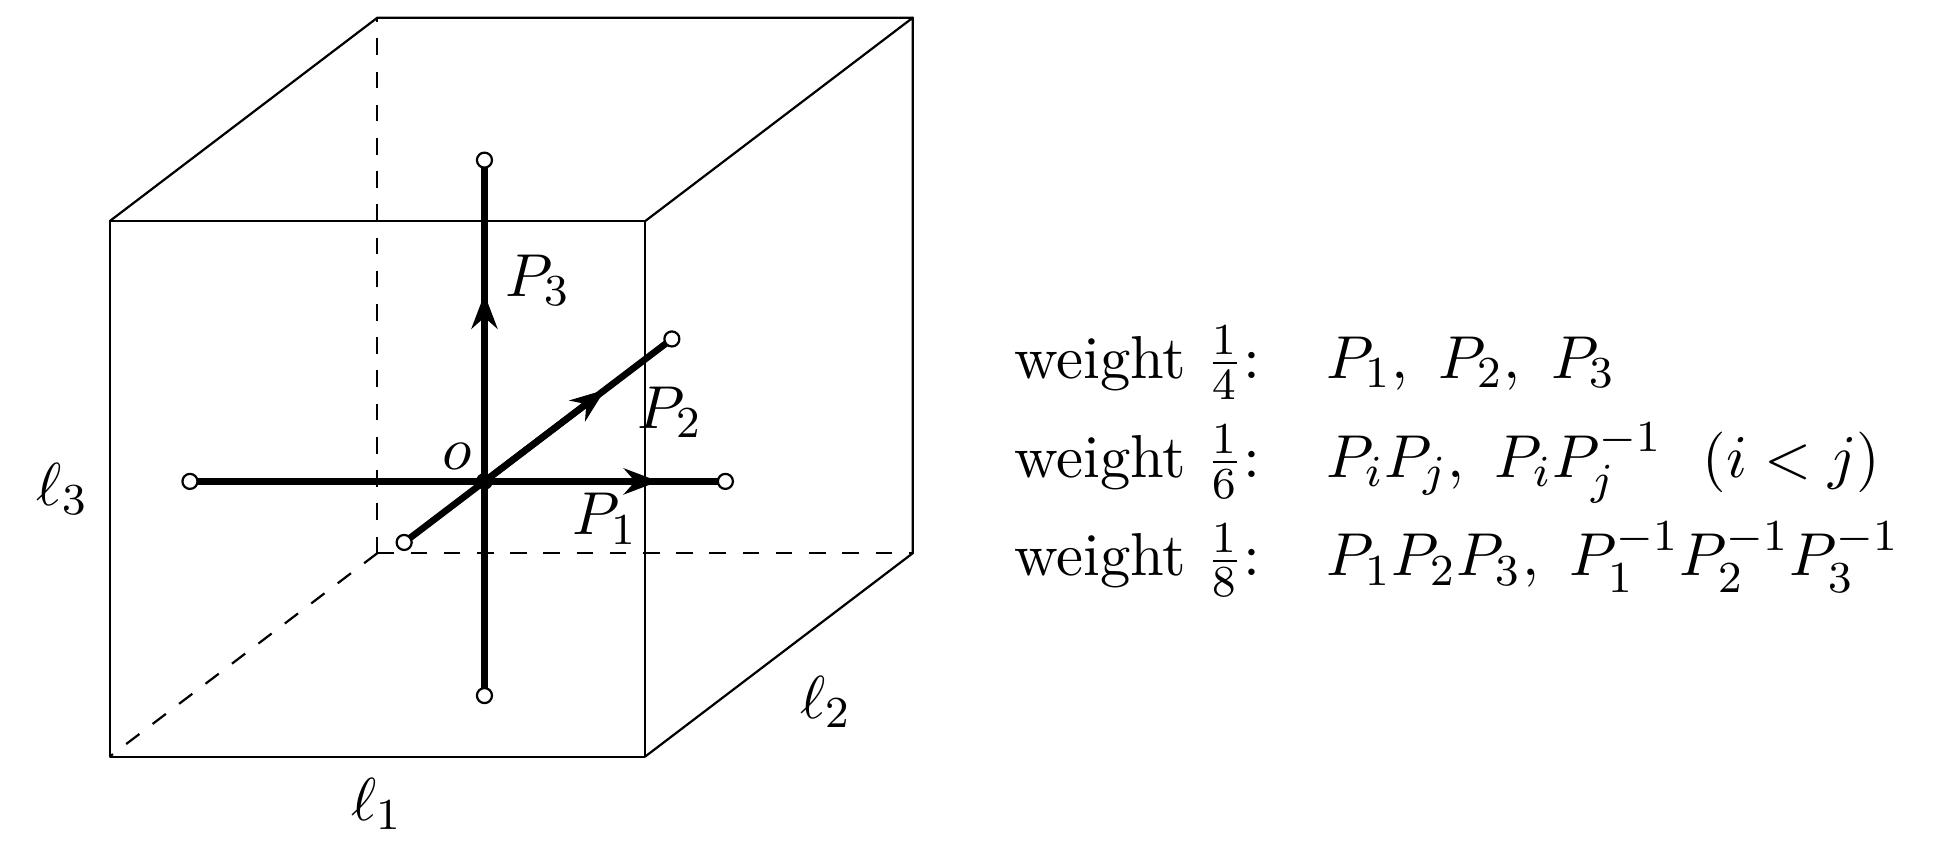
\includegraphics[width=348.6bp]{figures/fig16.png}
\caption{Left: the spatial torus $t=(\ell_1,\ell_2,\ell_3)$ drawn as a box whose opposite faces are identified, and the three holonomies $P_1,P_2,P_3$ based at the site $o$. The two open endpoints of each segment are the same site, so each loop winds once around one cycle and is not contractible. Right: the eleven charged words of \cref{lem:lemma-W}, grouped by weight; their traces are listed in \cref{tab:charged-words}.}
\label{fig:holonomies}
\end{figure}

\begin{table}[htbp]
\centering
\caption{The eleven charged words for $N=2$. Here $1\le i<j\le3$, the traces are written in the coordinates \eqref{eq:lw-coordinates}, $m_W$ is the length of the lattice loop at $o$ that realises $W$, and the last column lists the flips that change the sign of $\Tr W(P)$.}
\label{tab:charged-words}
\begin{tabular}{@{}lccccc@{}}
\toprule
word $W$ & number & weight $w_W$ & $\Tr W(P)$ & $m_W$ & odd under\\
\midrule
$P_i$ & $3$ & $1/4$ & $2a_i$ & $\ell_i$ & $z_i$\\
$P_iP_j$ & $3$ & $1/6$ & $2(a_ia_j-g_{ij})$ & $\ell_i+\ell_j$ & $z_i,z_j$\\
$P_iP_j^{-1}$ & $3$ & $1/6$ & $2(a_ia_j+g_{ij})$ & $\ell_i+\ell_j$ & $z_i,z_j$\\
$P_1P_2P_3$ & $1$ & $1/8$ & $2(s+d)$ & $\ell_1+\ell_2+\ell_3$ & $z_1,z_2,z_3$\\
$P_1^{-1}P_2^{-1}P_3^{-1}$ & $1$ & $1/8$ & $2(s-d)$ & $\ell_1+\ell_2+\ell_3$ & $z_1,z_2,z_3$\\
\bottomrule
\end{tabular}
\end{table}

\subsection{The eleven charged words}
Let $\sigma=(\sigma_1,\sigma_2,\sigma_3)$ be the Pauli matrices. Every element of $\SU(2)$ is a unit quaternion, and we write
\begin{equation}\label{eq:lw-coordinates}
P_k=a_k+i\,b_k\cdot\sigma,\qquad(a_k,b_k)\in\R\times\R^3,\qquad a_k^2+\abs{b_k}^2=1\qquad(k=1,2,3),
\end{equation}
and put
\begin{gather*}
g_{ij}=b_i\cdot b_j,\qquad d=\det(b_1,b_2,b_3),\qquad A=\sum_ka_k^2,\qquad S=\sum_{i<j}g_{ij}^2,\\
s=a_1a_2a_3-a_1g_{23}-a_2g_{13}-a_3g_{12}.
\end{gather*}
For $u,v\in\R^3$ one has $(iu\cdot\sigma)(iv\cdot\sigma)=-u\cdot v-i(u\times v)\cdot\sigma$, while $\Tr1=2$ and $\Tr\sigma_k=0$. Hence, for $i\neq j$,
\[
P_iP_j=(a_ia_j-g_{ij})+i\,(a_ib_j+a_jb_i-b_i\times b_j)\cdot\sigma ,
\]
and since $P_j^{-1}=P_j^{*}=a_j-i\,b_j\cdot\sigma$ arises from $P_j$ by $b_j\mapsto-b_j$,
\begin{equation}\label{eq:lw-traces}
\Tr P_k=2a_k,\qquad\Tr P_iP_j^{\pm1}=2(a_ia_j\mp g_{ij})\qquad(i\neq j).
\end{equation}
Multiplying $P_1P_2$ by $P_3$ and taking the trace gives
$\Tr P_1P_2P_3=2[(a_1a_2-g_{12})a_3-(a_1b_2+a_2b_1-b_1\times b_2)\cdot b_3]=2(s+d)$, because $(b_1\times b_2)\cdot b_3=d$. Every $U\in\SU(2)$ has real trace and $\Tr U^{-1}=\overline{\Tr U}$, so $\Tr P_1^{-1}P_2^{-1}P_3^{-1}=\Tr P_3P_2P_1$; the same computation with the indices reversed gives $2(s+\det(b_3,b_2,b_1))$. As $s$ is symmetric in the indices and the determinant is alternating,
\begin{equation}\label{eq:lw-triple}
\Tr P_1P_2P_3=2(s+d),\qquad\Tr P_1^{-1}P_2^{-1}P_3^{-1}=2(s-d).
\end{equation}

For $N=2$ the eleven words of \cref{tab:charged-words} are charged: each contains each of its letters exactly once, so its trace is odd under the flip of each of its letters. Their weighted sum of squared traces is
\begin{equation}\label{eq:lw-phi}
\begin{split}
\Phi(P)={}&\frac14\sum_i(\Tr P_i)^2+\frac16\sum_{i<j}\bigl[(\Tr P_iP_j)^2+(\Tr P_iP_j^{-1})^2\bigr]\\
&+\frac18\bigl[(\Tr P_1P_2P_3)^2+(\Tr P_1^{-1}P_2^{-1}P_3^{-1})^2\bigr],
\end{split}
\end{equation}
and \cref{lem:lemma-W} asserts that $\Phi\ge1$ on $\SU(2)^3$, with equality in particular at the three configurations
(i) $(i\sigma_1,i\sigma_2,i\sigma_3)$, (ii) $(1,i\sigma_1,i\sigma_2)$ and (iii) $(i\,n_1\cdot\sigma,i\,n_2\cdot\sigma,i\,n_3\cdot\sigma)$ with coplanar unit vectors $n_1,n_2,n_3$ at mutual angles $2\pi/3$.

\begin{proof}[Proof of \cref{lem:lemma-W}]
\emph{Gram expansion.} By \eqref{eq:lw-traces} and \eqref{eq:lw-triple}, $\frac14(\Tr P_k)^2=a_k^2$,
\[
\tfrac16\bigl[(\Tr P_iP_j)^2+(\Tr P_iP_j^{-1})^2\bigr]=\tfrac23\bigl[(a_ia_j-g_{ij})^2+(a_ia_j+g_{ij})^2\bigr]=\tfrac43\bigl(a_i^2a_j^2+g_{ij}^2\bigr),
\]
and $\frac18[4(s+d)^2+4(s-d)^2]=s^2+d^2$. Hence
\begin{equation}\label{eq:lw-gram}
\Phi=A+\frac43\sum_{i<j}a_i^2a_j^2+\frac43S+s^2+d^2 .
\end{equation}
Let $B$ be the real $3\times3$ matrix with columns $b_1,b_2,b_3$ and $G=B^{\mathsf T}B=(g_{ij})$ their Gram matrix. Then $d^2=(\det B)^2=\det G$, and dropping the nonnegative terms $\frac43\sum_{i<j}a_i^2a_j^2$ and $s^2$ gives
\begin{equation}\label{eq:lw-first}
\Phi\ \ge\ A+\tfrac43S+\det G .
\end{equation}

\emph{Lower bound for $\det G$.} The diagonal entries of $G$ are $p_k=\abs{b_k}^2=1-a_k^2\in[0,1]$, and
\[
\det G=p_1p_2p_3+2g_{12}g_{13}g_{23}-p_1g_{23}^2-p_2g_{13}^2-p_3g_{12}^2 .
\]
We bound the three groups of terms. First, $\prod_k(1-x_k)\ge1-\sum_kx_k$ for $x_k\in[0,1]$, by induction on the number of factors and $(1-X)(1-x)\ge1-X-x$ for $X,x\ge0$; hence $p_1p_2p_3\ge1-A$. Second, the arithmetic--geometric mean inequality for $g_{12}^2,g_{13}^2,g_{23}^2$ gives $\abs{g_{12}g_{13}g_{23}}\le(S/3)^{3/2}$. Third, $p_k\le1$ gives $p_1g_{23}^2+p_2g_{13}^2+p_3g_{12}^2\le S$. Therefore
\begin{equation}\label{eq:lw-det-bound}
\det G\ \ge\ 1-A-\kappa(S),\qquad\kappa(S)=S+2\Bigl(\frac S3\Bigr)^{3/2}.
\end{equation}
The function $\kappa$ is increasing on $[0,\infty)$, and $\kappa(3/4)=\frac34+2\cdot\frac18=1$.

\emph{Three cases.} Since $\det G=d^2\ge0$, \eqref{eq:lw-first} and \eqref{eq:lw-det-bound} give
\[
\Phi\ \ge\ h:=A+\tfrac43S+\max\{0,\,1-A-\kappa(S)\}.
\]
If $S\ge3/4$, then $h\ge\frac43S\ge1$. If $A+\kappa(S)\le1$, then $\kappa(S)\le1=\kappa(3/4)$, so $S\le3/4$, and $h=1+\frac S3-2(\frac S3)^{3/2}$. If $A+\kappa(S)>1$ and $S<3/4$, then $h\ge A+\frac43S>1-\kappa(S)+\frac43S=1+\frac S3-2(\frac S3)^{3/2}$. In the last two cases $0\le S\le3/4$, hence $(S/3)^{1/2}\le\frac12$ and
\[
h\ \ge\ 1+\frac S3\Bigl(1-2\Bigl(\frac S3\Bigr)^{1/2}\Bigr)\ \ge\ 1 .
\]
Thus $\Phi\ge1$ on $\SU(2)^3$.

\emph{Equality.} We evaluate \eqref{eq:lw-gram}. At (i), $a=0$ and $b_k=e_k$, so $A=S=s=0$ and $d=1$, and $\Phi=1$. At (ii), $a=(1,0,0)$, $b_1=0$, $b_2=e_1$, $b_3=e_2$, so $A=1$, every product $a_ia_j$ ($i<j$) and every $g_{ij}$ vanishes, $s=0$ and $d=0$, and $\Phi=1$. At (iii), $a=0$ and $b_k=n_k$, so $g_{ij}=\cos(2\pi/3)=-\frac12$, $S=\frac34$, $s=0$, and $d=0$ because the $n_k$ are coplanar; hence $\Phi=\frac43\cdot\frac34=1$.\footnote{Following the equalities through the proof identifies the whole set $\{\Phi=1\}$: it consists of the triples with $g_{ij}=0$ for all $i<j$ and at most one $a_k\neq0$, and of the triples with $a_1=a_2=a_3=0$ whose unit vectors $b_k$ are coplanar and span lines meeting pairwise at angle $\pi/3$. Indeed, if $S=0$ then $s=a_1a_2a_3$ and $d^2=\prod_k(1-a_k^2)$, and \eqref{eq:lw-gram} becomes $\Phi=1+\frac73\sum_{i<j}a_i^2a_j^2$; if $S>3/4$ or $0<S<3/4$ the three cases give $\Phi>1$; if $S=3/4$ then \eqref{eq:lw-first} gives $\Phi\ge1+A+d^2$, so $A=d=0$, and coplanar unit vectors at angles $\theta_1,\theta_2,\theta_3$ in their plane have $S=\frac34+\frac14\abs{\sum_ke^{2i\theta_k}}^2$, so $S=\frac34$ exactly when the doubled angles $2\theta_1,2\theta_2,2\theta_3$ are equally spaced on the circle. The set contains the curve $(\cos\theta+i\sin\theta\,\sigma_3,\,i\sigma_1,\,i\sigma_2)$, which joins (ii) to a permutation of (i).}
\end{proof}

In the proof of \cref{thm:fixed-torus-gap} each word $W$ is realised by a closed lattice loop at $o$ of length $m_W$ (\cref{tab:charged-words}), and the constant in front of $\varepsilon(c)$ is $2\sum_Ww_Wm_W^2$. By the table,
\begin{equation}\label{eq:lw-lengths}
\begin{split}
2\sum_Ww_Wm_W^2&=\frac12\sum_i\ell_i^2+\frac23\sum_{i<j}(\ell_i+\ell_j)^2+\frac12(\ell_1+\ell_2+\ell_3)^2\\
&\le\Bigl(\frac12+\frac83+\frac32\Bigr)\sum_i\ell_i^2=\frac{14}{3}\sum_i\ell_i^2,
\end{split}
\end{equation}
where the inequality uses $(\ell_i+\ell_j)^2\le2(\ell_i^2+\ell_j^2)$, each index lying in two pairs, and $(\ell_1+\ell_2+\ell_3)^2\le3\sum_i\ell_i^2$. On the cube $\ell_1=\ell_2=\ell_3=\ell$ both sides of \eqref{eq:lw-lengths} equal $14\ell^2$. No weighting of the eleven words that is constant on words of equal length does better on the cube: with weights $\alpha_1,\alpha_2,\alpha_3$ on the words of length one, two and three, the weighted sum $\Phi_\alpha$ of squared traces equals $8\alpha_3$, $4\alpha_1$ and $6\alpha_2$ at (i), (ii) and (iii), so $\min\Phi_\alpha\le\mu:=\min\{4\alpha_1,6\alpha_2,8\alpha_3\}$, and the cube constant $2\sum_W\alpha_{\abs{W}}m_W^2/\min\Phi_\alpha$ is at least $2\sum_W\alpha_{\abs{W}}m_W^2/\mu=(6\alpha_1+48\alpha_2+36\alpha_3)\ell^2/\mu\ge(\frac64+\frac{48}6+\frac{36}8)\ell^2=14\ell^2$.

\begin{remark}
Three holonomies are needed. The pair $(P_1,P_2)=(i\sigma_1,i\sigma_2)$ generates the quaternion group $\{\pm1,\pm i\sigma_1,\pm i\sigma_2,\pm i\sigma_3\}$, whose quotient by $\{\pm1\}$ is $\Z_2\times\Z_2$; the image of a word in the quotient is determined by $(n_1,n_2)\bmod2$, so every word with $n_1$ or $n_2$ odd is sent to some $\pm i\sigma_k$ and is traceless. All charged traces in two letters vanish at this point, and no inequality of the type of \cref{lem:lemma-W} holds for two holonomies. This is why the two-holonomy argument of \cite[Theorem~8]{bhattacharjee2026first} needs the near-flatness condition $(\ell_1\ell_2)^2\varepsilon(c)<3$, which \cref{thm:fixed-torus-gap} does not need. Here $g_1=i\sigma_2$ and $g_2=i\sigma_1$ conjugate $(P_1,P_2)$ to $(-P_1,P_2)$ and to $(P_1,-P_2)$; the no-triple-twist lemma below excludes this for three letters.
\end{remark}

\subsection{Three holonomies in \texorpdfstring{$\SU(N)$}{SU(N)}}
Let $N\ge2$ and $\omega=e^{2\pi i/N}$. The no-triple-twist lemma is the $\SU(N)$ form of the last remark, the equal-traces lemma turns equal traces into a conjugacy, and the charged-lower-bound lemma combines the two into a uniform lower bound by compactness. A triple $P\in\SU(N)^3$ is \emph{twistable in direction $j$} if some $g_j\in\mathrm{GL}_N(\C)$ satisfies
\begin{equation}\label{eq:lw-twist}
g_jP_jg_j^{-1}=\omega P_j,\qquad g_jP_ig_j^{-1}=P_i\quad(i\neq j).
\end{equation}

\begin{lemma}[No triple twist]
No triple $P\in\SU(N)^3$ is twistable in all three directions.
\end{lemma}

\begin{proof}
Suppose that $g_1,g_2,g_3$ satisfy \eqref{eq:lw-twist}.

\emph{Distinct eigenvalues.} The spectrum of $P_1$, counted with multiplicity, is a multiset of $N$ points of the unit circle; it is invariant under multiplication by $\omega$ because $P_1$ is similar to $\omega P_1$. Multiplication by powers of $\omega$ is a free action of $\Z_N$ on the circle with orbits of $N$ points, and the multiplicity function is constant on orbits. Hence the spectrum is one orbit $\{\lambda\omega^k:0\le k<N\}$ and every eigenvalue is simple. Let $e_k$ be an eigenvector for $\lambda\omega^k$, indices modulo $N$.

\emph{$g_1$ is a weighted cyclic shift.} By \eqref{eq:lw-twist}, $P_1g_1=\omega^{-1}g_1P_1$, so $P_1(g_1e_k)=\lambda\omega^{k-1}g_1e_k$. The eigenspace of $\lambda\omega^{k-1}$ is the line $\C e_{k-1}$, hence $g_1e_k=c_ke_{k-1}$, and $c_k\neq0$ because $g_1$ is invertible. Therefore $g_1^N=c\,1$ with $c=\prod_kc_k\neq0$, and $e_0$ is a cyclic vector for $g_1$. The minimal polynomial of $g_1$ has degree $N$ and divides $x^N-c$, so it equals $x^N-c$, whose $N$ roots are distinct: $g_1$ has $N$ distinct eigenvalues.

\emph{Commutation.} A matrix commuting with $g_1$ preserves each eigenline of $g_1$, so the commutant of $g_1$ consists of the matrices diagonal in an eigenbasis of $g_1$, and it is commutative. By \eqref{eq:lw-twist}, $P_2$ and $P_3$ commute with $g_1$; hence $P_2P_3=P_3P_2$. The same argument with $g_2$ and with $g_3$ gives $P_1P_3=P_3P_1$ and $P_1P_2=P_2P_1$.

\emph{Joint spectrum.} Commuting unitary matrices are simultaneously diagonalisable, so $\C^N$ is the direct sum of the joint eigenspaces $E(\mu)=\{v:P_jv=\mu_jv,\ j=1,2,3\}$, $\mu\in(S^1)^3$, and $\sum_\mu\dim E(\mu)=N$. If $v\in E(\mu)$, then \eqref{eq:lw-twist} gives $g_1v\in E(\omega^{-1}\mu_1,\mu_2,\mu_3)$, and $g_1^{-1}$ maps $E(\omega^{-1}\mu_1,\mu_2,\mu_3)$ into $E(\mu)$; so $\dim E(\mu)=\dim E(\omega^{-1}\mu_1,\mu_2,\mu_3)$, and in the same way for the second and third coordinates. The function $\mu\mapsto\dim E(\mu)$ is therefore invariant under the action of $\Z_N^3$ by coordinatewise multiplication with powers of $\omega$. This action is free with orbits of $N^3$ points, so $N=\sum_\mu\dim E(\mu)$ is a positive multiple of $N^3$, which is impossible for $N\ge2$.
\end{proof}

\begin{lemma}[Equal traces]
Let $\rho,\rho'$ be unitary representations of a group $\Gamma$ on $\C^N$ with $\Tr\rho(\gamma)=\Tr\rho'(\gamma)$ for all $\gamma\in\Gamma$. Then $\rho$ and $\rho'$ are equivalent: some $g\in\mathrm{GL}_N(\C)$ satisfies $g\rho(\gamma)g^{-1}=\rho'(\gamma)$ for all $\gamma\in\Gamma$.
\end{lemma}

\begin{proof}
Let $K$ be the closure of $\{(\rho(\gamma),\rho'(\gamma)):\gamma\in\Gamma\}$ in $\U(N)\times\U(N)$. It is a closed subgroup of a compact group, hence compact; let $\dd k$ be its normalised Haar measure, and let $\pi,\pi'$ be the two coordinate representations of $K$ on $\C^N$, with characters $\chi,\chi'$. These agree on the dense subset $\{(\rho(\gamma),\rho'(\gamma))\}$, hence on $K$. For a finite-dimensional continuous unitary representation $\tau$ of $K$ on a space $V$, the operator $\int_K\tau(k)\dd k$ is the orthogonal projection onto the invariant vectors $V^K$, so $\int_K\Tr\tau(k)\dd k=\dim V^K$. Apply this to the space of linear maps $X:\C^N\to\C^N$, on which $K$ acts by $X\mapsto\pi_b(k)X\pi_a(k)^{-1}$ for $\pi_a,\pi_b\in\{\pi,\pi'\}$; the character of this action is $\chi_b\overline{\chi_a}$, and its invariant vectors are the intertwiners from $\pi_a$ to $\pi_b$. Hence
\[
\dim\operatorname{Hom}_K(\pi_a,\pi_b)=\int_K\chi_b(k)\,\overline{\chi_a(k)}\dd k ,
\]
and the right side is the same for all four pairs because $\chi=\chi'$. Decompose $\pi\cong\bigoplus_km_k\eta_k$ and $\pi'\cong\bigoplus_kn_k\eta_k$ into pairwise inequivalent irreducible representations $\eta_k$. By Schur's lemma, $\dim\operatorname{Hom}_K(\pi,\pi)=\sum_km_k^2$, $\dim\operatorname{Hom}_K(\pi,\pi')=\sum_km_kn_k$ and $\dim\operatorname{Hom}_K(\pi',\pi')=\sum_kn_k^2$. These are equal, so $\sum_k(m_k-n_k)^2=0$ and $m_k=n_k$ for all $k$. Thus $\pi\cong\pi'$, and an invertible intertwiner $g$ satisfies $g\pi(k)=\pi'(k)g$ on $K$, in particular $g\rho(\gamma)g^{-1}=\rho'(\gamma)$.
\end{proof}

\begin{lemma}[Charged lower bound]
Let $\mathcal{C}_N$ be the set of charged words, $n(W)\not\equiv0\pmod N$. There are a finite set $\mathcal{F}_N\subset\mathcal{C}_N$ and a constant $\gamma_N>0$ such that
\begin{equation}\label{eq:lw-charged-bound}
\Phi_{\mathcal{F}_N}(P):=\sum_{W\in\mathcal{F}_N}\abs{\Tr W(P)}^2\ \ge\ \gamma_N\qquad\text{for all }P\in\SU(N)^3 .
\end{equation}
\end{lemma}

\begin{proof}
Let $P\in\SU(N)^3$ and suppose that $\Tr W(P)=0$ for every $W\in\mathcal{C}_N$. Define unitary representations $\rho,\rho_1,\rho_2,\rho_3$ of $F_3$ on $\C^N$ by $\rho(x_i)=P_i$ and $\rho_j(x_i)=\omega^{\delta_{ij}}P_i$. By \eqref{eq:lw-flip}, $\Tr\rho_j(W)=\omega^{n_j(W)}\Tr\rho(W)$ for every word $W$. If $n_j(W)\equiv0\pmod N$ the two traces are equal; otherwise $W\in\mathcal{C}_N$ and both vanish. So $\rho_j$ and $\rho$ have equal traces, and the equal-traces lemma gives $g_j\in\mathrm{GL}_N(\C)$ with $g_j\rho(\gamma)g_j^{-1}=\rho_j(\gamma)$ for all $\gamma\in F_3$; on the generators this is \eqref{eq:lw-twist}. Since this holds for $j=1,2,3$, it contradicts the no-triple-twist lemma. Hence the closed sets $\{P\in\SU(N)^3:\Tr W(P)=0\}$, $W\in\mathcal{C}_N$, have empty intersection. As $\SU(N)^3$ is compact, finitely many of them, say those with $W\in\mathcal{F}_N$, already have empty intersection. Then $\Phi_{\mathcal{F}_N}$ is continuous and strictly positive on the compact set $\SU(N)^3$, and its minimum $\gamma_N$ is positive.
\end{proof}

For $N=2$ the eleven words of \cref{tab:charged-words} satisfy \eqref{eq:lw-charged-bound} with $\mathcal{F}_2$ the eleven words and $\gamma_2=4$, since every weight in \eqref{eq:lw-phi} is at most $\frac14$ and so $\sum_W(\Tr W(P))^2\ge4\Phi(P)\ge4$; the value $4$ is attained at (ii). For $N\ge3$ compactness gives no value of $\gamma_N$, and the constant $K_N$ of \cref{thm:SUN-gap}, built from $\mathcal{F}_N$ and $\gamma_N$, is not explicit. In that theorem the real and imaginary parts of $\Tr W(P)$, $W\in\mathcal{F}_N$, replace the eleven traces, and \eqref{eq:lw-charged-bound} replaces $\Phi\ge1$.
\section{The harmonic (free-gluon) reference}\label{app:harmonic}

This appendix defines the reference system $\Gharm$ used in \cref{prop:no-stefan-boltzmann,thm:free-gluon,thm:pair,thm:universal-step}, computes its spectrum and thermal traces, and exhibits the twelve two-gluon colour singlets of \cref{prop:no-stefan-boltzmann}. The system $\Gharm$ is a family of explicit operators $R_{\Gharm}(s)$, one for each triple $s=(s_1,s_2,s_3)$ of sides $s_j\ge2$, which play the role of the normalised transfer matrix $R=\TT_s/\lzero$ of \cref{sec:psts} on $\Lambda_s\times\Z$. It is not the Wilson transfer matrix, and no statement about $\Gharm$ is a statement about the Wilson measure.\footnote{By \cite[Proposition~38 and its proof, Lemma~47]{bhattacharjee2026first}, the transfer operator of $N^2-1$ independent Gaussian lattice Maxwell fields on $\Lambda_s$ is a tensor product of one-mode kernels with eigenvalues $\sqrt{2\pi}\,e^{-\omega_p/2}e^{-j\omega_p}$, $j\ge0$, two for each colour and each nonzero momentum $p$, and of kernels for the constant modes. Without the latter and normalised, it has the spectrum of $R_{\Gharm}(s)$ (\cref{lem:harmonic-spectrum}). This explains the name and is used in no proof.}

Throughout this appendix, $N\ge2$ is the number of colours (the matrix size $N_c$ of \cref{sec:psts}; the mesh index plays no role here), $\mathfrak g=\mathfrak{su}(N)$ carries the real, positive definite, $\mathrm{Ad}$-invariant inner product $\ip{X}{Y}=-\tr(XY)$, $(t_a)_{a=1}^{N^2-1}$ is an orthonormal basis of $\mathfrak g$, and $\mathfrak g_\C=\mathfrak{sl}(N,\C)$ carries $\ip{X}{Y}=\tr(X^*Y)$. For a triple $s=(s_1,s_2,s_3)$ of integers $s_j\ge2$ let $\Lambda_s=\Z_{s_1}\times\Z_{s_2}\times\Z_{s_3}$, so $\abs{\Lambda_s}=\Vol{s}$, and $\Lambda_s^*=\{(2\pi n_j/s_j)_{j=1}^3:n\in\Lambda_s\}$. For $p\in\Lambda_s^*$ define $\lambda_p\ge0$ and $\omega_p\ge0$ by
\[
 \lambda_p=\sum_{j=1}^34\sin^2\frac{p_j}2=\sum_{j=1}^34\sin^2\frac{\pi n_j}{s_j},\qquad 4\sinh^2\frac{\omega_p}2=\lambda_p ;
\]
$\omega_p>0$ for $p\ne0$. A vector field is a map $A=(A_1,A_2,A_3):\Lambda_s\to\mathfrak g^3$, $A_j(x)$ sitting on the link from $x$ to $x+e_j$, with the inner product $\sum_x\sum_j\ip{A_j(x)}{A'_j(x)}$, the divergence and the componentwise Laplacian
\[
 (\operatorname{div}A)(x)=\sum_j\bigl(A_j(x)-A_j(x-e_j)\bigr),\qquad (-\Delta A)_j(x)=\sum_{l=1}^3\bigl(2A_j(x)-A_j(x+e_l)-A_j(x-e_l)\bigr).
\]

\begin{definition}[the harmonic reference $\Gharm$]\label{def:harmonic}
Let $s$ have sides $\ge2$.
\begin{enumerate}[label=(\roman*)]
\item $\mathfrak h^{\R}_s=\{A:\operatorname{div}A=0,\ \sum_xA_j(x)=0\ (j=1,2,3)\}$ is the space of transverse fields with the zero mode removed, and $\mathfrak h_s=\mathfrak h^{\R}_s\otimes\C$, with the complex conjugation $J$ fixing $\mathfrak h^{\R}_s$. Both $-\Delta$ and $\operatorname{div}$ are built from translations acting componentwise, so they commute, and $\sum_x(-\Delta A)_j(x)=0$; hence $-\Delta$ maps $\mathfrak h^{\R}_s$ into itself. Its restriction $-\Delta_\perp$ is nonnegative, since $\ip{A}{-\Delta A}=\sum_{x,j,l}\abs{A_j(x+e_l)-A_j(x)}^2$, and $\omega_s=2\operatorname{arsinh}\bigl(\tfrac12(-\Delta_\perp)^{1/2}\bigr)$. The same symbols denote complex-linear extensions to $\mathfrak h_s$.
\item On the bosonic Fock space $\mathcal F(\mathfrak h_s)$, with vacuum $\Omega$ and creation operators $a^\dagger(f)$, put $R_{\Gharm}(s)=\Gamma(e^{-\omega_s})$, where $\Gamma(B)\,a^\dagger(f_1)\cdots a^\dagger(f_n)\Omega=a^\dagger(Bf_1)\cdots a^\dagger(Bf_n)\Omega$ for a contraction $B$ of $\mathfrak h_s$. An eigenvalue $e^{-E}$ of $R_{\Gharm}(s)$ has energy $E$.
\item For integers $T\ge1$: $\Zs{\Gharm,s}{T}=\Tr R_{\Gharm}(s)^T$, $\XT{\Gharm,s}{T}=\log\Zs{\Gharm,s}{T}$, $\psiT{\Gharm,s}{T}=2\XT{\Gharm,s}{T}-\XT{\Gharm,s}{2T}$, and on the cube $\XT{\Gharm}{T}=\XT{\Gharm,\cube{T}}{T}$, $\psiT{\Gharm}{T}=\psiT{\Gharm,\cube{T}}{T}$.
\end{enumerate}
\end{definition}

For a \PSTS{} the factors $\lzero^{2T}$ cancel in $2\log\Zpart{s}{T}-\log\Zpart{s}{2T}$, so $\psiT{s}{T}=2\XT{s}{T}-\XT{s}{2T}$, the expression used in (iii).

\begin{lemma}[spectrum, traces and symmetries]\label{lem:harmonic-spectrum}
Let $s$ have sides $\ge2$.
\begin{enumerate}[label=(\roman*)]
\item For $p\in\Lambda_s^*\setminus\{0\}$ let $E_p\subset\mathfrak h_s$ be spanned by the fields $e^{ip\cdot x}(\varepsilon_1X,\varepsilon_2X,\varepsilon_3X)$ with $X\in\mathfrak g_\C$, $\varepsilon\in\C^3$ and $\sum_j(1-e^{-ip_j})\varepsilon_j=0$. Then $\dim_\C E_p=2(N^2-1)$, $\mathfrak h_s=\bigoplus_{p\ne0}E_p$ orthogonally, and $\omega_s=\omega_p$ on $E_p$. So $\omega_s>0$, and its eigenvalues listed with multiplicity are the numbers $\omega_p$, $p\in\Lambda_s^*\setminus\{0\}$, each repeated $2(N^2-1)$ times.
\item $R_{\Gharm}(s)\ge0$ is trace class, its largest eigenvalue $1$ is simple with eigenvector $\Omega$, and for $T\ge1$
\begin{equation}\label{eq:harmonic-traces}
\begin{gathered}
 \XT{\Gharm,s}{T}=-2(N^2-1)\sum_{p\in\Lambda_s^*\setminus\{0\}}\log\bigl(1-e^{-T\omega_p}\bigr),\\
 \psiT{\Gharm,s}{T}=2(N^2-1)\sum_{p\in\Lambda_s^*\setminus\{0\}}2\operatorname{artanh}e^{-T\omega_p} .
\end{gathered}
\end{equation}
\item The translations $(\tau_yA)(x)=A(x-y)$, the global colour rotations $A\mapsto gAg^{-1}$ ($g\in\SU(N)$), the charge conjugation $A\mapsto-A^{\mathsf T}$ and, if $s$ is a cube, the axis permutations $(\pi A)_{\pi(j)}(\pi x)=A_j(x)$ and the reflections $(r_kA)_k(x)=-A_k(r_kx-e_k)$, $(r_kA)_j(x)=A_j(r_kx)$ ($j\ne k$), $r_kx=x-2x_ke_k$, are real orthogonal maps of $\mathfrak h^{\R}_s$ commuting with $\omega_s$; their complex-linear extensions commute with $J$, and their second quantisations commute with $R_{\Gharm}(s)$. Central elements of $\SU(N)$ act as the identity.
\item If $s=(L,L,L)$, $L\ge3$, the smallest eigenvalue of $\omega_s$ is $\omega_1(L)=2\operatorname{arsinh}(\sin\frac\pi L)\le\frac{2\pi}L$, with eigenspace $\bigoplus E_p$ over the six momenta $p=\pm\frac{2\pi}Le_j$, of dimension $12(N^2-1)$. On $\cube{T}$, $T\ge2$, the lowest shell has $T\omega_1(2T)\le\pi$.
\end{enumerate}
\end{lemma}

\begin{proof}
(i) Expand $A(x)=\Vol{s}^{-1/2}\sum_{p\in\Lambda_s^*}e^{ip\cdot x}\hat A(p)$ with $\hat A(p)\in\mathfrak g_\C^3$; plane waves of distinct momenta are orthogonal. Termwise, $\operatorname{div}$ multiplies $\hat A(p)$ by the row vector $w(p)=(1-e^{-ip_j})_j$, $-\Delta$ multiplies it by $\sum_l(2-2\cos p_l)=\lambda_p$, and $\sum_xA_j(x)=\Vol{s}^{1/2}\hat A_j(0)$. Hence $\mathfrak h_s=\bigoplus_{p\ne0}E_p$ and $-\Delta_\perp=\lambda_p$, $\omega_s=\omega_p>0$ on $E_p$. For $p\ne0$ some $p_j\not\equiv0$, so $w(p)\ne0$; writing $\hat A(p)=\sum_a\varepsilon^{(a)}t_a$, the condition $w(p)\cdot\varepsilon^{(a)}=0$ leaves two dimensions for each $a$.

(ii) Let $(\chi_r)_{r=1}^D$, $D=2(N^2-1)(\Vol{s}-1)$, be an orthonormal eigenbasis of $\omega_s$ with eigenvalues $\varpi_r>0$. The normalised vectors $\prod_ra^\dagger(\chi_r)^{\nu_r}\Omega$, $\nu\in\{0,1,2,\dots\}^D$, form an orthonormal basis of $\mathcal F(\mathfrak h_s)$ on which $R_{\Gharm}(s)$ acts by $e^{-E_\nu}$, $E_\nu=\sum_r\nu_r\varpi_r$. So $R_{\Gharm}(s)\ge0$, the eigenvalue $1$ occurs only at $\nu=0$, and $\Zs{\Gharm,s}{T}=\prod_r(1-e^{-T\varpi_r})^{-1}<\infty$. With (i) this is the formula for $X$; for $\psi$, each $r$ contributes $-2\log(1-q)+\log(1-q^2)=2\operatorname{artanh}q$, $q=e^{-T\varpi_r}$.

(iii) Each map is orthogonal and preserves the conditions $\sum_xA_j(x)=0$. Translations commute with $\operatorname{div}$ and $-\Delta$, and colour rotations and charge conjugation act on the values only; for the latter, $-X^{\mathsf T}=\bar X\in\mathfrak g$ and $\ip{-X^{\mathsf T}}{-Y^{\mathsf T}}=-\tr(YX)=\ip{X}{Y}$ for $X,Y\in\mathfrak g$. For $\pi$ and $r_k$ direct substitution gives $\operatorname{div}(\pi A)(\pi x)=(\operatorname{div}A)(x)$, $\operatorname{div}(r_kA)(x)=(\operatorname{div}A)(r_kx)$, and $-\Delta(\pi A)=\pi(-\Delta A)$, $-\Delta(r_kA)=r_k(-\Delta A)$; for instance $(r_kA)_k(x)-(r_kA)_k(x-e_k)=A_k(r_kx)-A_k(r_kx-e_k)$. So every map preserves $\mathfrak h^{\R}_s$ and commutes with $-\Delta_\perp$, hence with $\omega_s$; real maps commute with $J$, and $\Gamma(U)\Gamma(e^{-\omega_s})=\Gamma(Ue^{-\omega_s})=\Gamma(e^{-\omega_s})\Gamma(U)$.

(iv) With representatives $\abs{n_j}\le L/2$, every $p\ne0$ has some $n_j\ne0$ and $\sin^2(\pi n_j/L)\ge\sin^2(\pi/L)$, with equality iff $n_j=\pm1$. So $\lambda_p\ge4\sin^2(\pi/L)$, with equality exactly at the six momenta (distinct as $L\ge3$), and $\omega_p$ increases with $\lambda_p$. Finally $\operatorname{arsinh}y\le y$ and $\sin y\le y$ for $y\ge0$.
\end{proof}

On the cube, \eqref{eq:harmonic-traces} reads $\XT{\Gharm}{T}=-2(N^2-1)\sum_{n\in\Z_{2T}^3\setminus\{0\}}\log(1-e^{-T\omega_n})$ with $4\sinh^2(\omega_n/2)=\sum_j4\sin^2(\pi n_j/2T)$. The bounds on $\XT{\Gharm}{T}$ and $\psiT{\Gharm}{T}$ are proved in \cref{thm:free-gluon}.\footnote{Numerically, as a sanity check entering no proof (\cref{app:verification}), $\XT{\Gharm}{T}/(N^2-1)=2.2063$, $1.6520$, $1.2187$, $1.1015$ at $T=3,4,6,8$; since $T\omega_n\to\pi\abs n$ for fixed $n$, the sum of the termwise limits is $-2(N^2-1)\sum_{n\in\Z^3\setminus\{0\}}\log(1-e^{-\pi\abs n})=0.984703\,(N^2-1)$.}

\begin{lemma}[the twelve two-gluon colour singlets]\label{lem:two-gluon-singlets}
Let $T\ge2$, $s=\cube{T}$, $\omega_1=2\operatorname{arsinh}(\sin\frac\pi{2T})$, $p_j=\frac\pi Te_j$, and $\varepsilon^{(j,\lambda)}=e_{j+\lambda}$ for $\lambda\in\{1,2\}$ (indices modulo $3$). Let $f^{\pm}_{j,\lambda,a}(x)=\Vol{s}^{-1/2}e^{\pm ip_j\cdot x}\,\varepsilon^{(j,\lambda)}t_a$ and, for $j\in\{1,2,3\}$ and $(\lambda,\lambda')\in\{1,2\}^2$,
\[
 \Phi_{j,\lambda,\lambda'}=\sum_{a=1}^{N^2-1}a^\dagger\bigl(f^{+}_{j,\lambda,a}\bigr)\,a^\dagger\bigl(f^{-}_{j,\lambda',a}\bigr)\,\Omega .
\]
\begin{enumerate}[label=(\roman*)]
\item Each $\Phi_{j,\lambda,\lambda'}$ is invariant under every $\Gamma(\mathrm{Ad}\,g)$, $g\in\SU(N)$ (colour singlet), and every $\Gamma(\tau_y)$, $y\in\Lambda_s$ (zero momentum).
\item $\ip{\Phi_{j,\lambda,\lambda'}}{\Phi_{k,\mu,\mu'}}=(N^2-1)\delta_{jk}\delta_{\lambda\mu}\delta_{\lambda'\mu'}$, and $\Phi_{j,\lambda,\lambda'}\perp\Omega$.
\item $R_{\Gharm}(s)\Phi_{j,\lambda,\lambda'}=e^{-2\omega_1}\Phi_{j,\lambda,\lambda'}$, and $2\omega_1\le2\pi/T$.
\item If $P$ projects onto the vectors invariant under all $\Gamma(\mathrm{Ad}\,g)$ and $\Gamma(\tau_y)$, then $P$ commutes with $R_{\Gharm}(s)$ and $\Tr(PR_{\Gharm}(s)^T)\ge1+12e^{-2T\omega_1}\ge1+12e^{-2\pi}$.
\end{enumerate}
\end{lemma}

\begin{proof}
As $T\ge2$, the six momenta $\pm p_j$ are nonzero and pairwise distinct modulo $2\pi$. Since $1-e^{\pm i(p_j)_l}$ vanishes for $l\ne j$ and $\varepsilon^{(j,\lambda)}_j=0$, $f^{\pm}_{j,\lambda,a}\in E_{\pm p_j}$, so $\omega_sf^{\pm}_{j,\lambda,a}=\omega_1f^{\pm}_{j,\lambda,a}$ by \cref{lem:harmonic-spectrum}(i); and the $f^{\pm}_{j,\lambda,a}$ are orthonormal (distinct momenta, or orthonormal polarisations and colours). This gives (iii), with \cref{lem:harmonic-spectrum}(iv) for $2T\omega_1\le2\pi$. (i): $\tau_yf^{\pm}_{j,\lambda,a}=e^{\mp ip_j\cdot y}f^{\pm}_{j,\lambda,a}$ and the phases cancel; $\mathrm{Ad}(g)t_a=\sum_bO_{ba}t_b$ with $O$ real orthogonal, so $\Gamma(\mathrm{Ad}\,g)\Phi_{j,\lambda,\lambda'}=\sum_{b,c}(OO^{\mathsf T})_{bc}a^\dagger(f^{+}_{j,\lambda,b})a^\dagger(f^{-}_{j,\lambda',c})\Omega=\Phi_{j,\lambda,\lambda'}$. (ii): $\ip{a^\dagger(f_1)a^\dagger(f_2)\Omega}{a^\dagger(g_1)a^\dagger(g_2)\Omega}=\ip{f_1}{g_1}\ip{f_2}{g_2}+\ip{f_1}{g_2}\ip{f_2}{g_1}$; the exchange terms vanish because $p_j\not\equiv-p_k$, and the direct terms give $\sum_{a,b}\delta_{jk}\delta_{\lambda\mu}\delta_{\lambda'\mu'}\delta_{ab}$. (iv): $\Gamma(\mathrm{Ad}\,g)$ and $\Gamma(\tau_y)$ commute with $R=R_{\Gharm}(s)$ (\cref{lem:harmonic-spectrum}(iii)), so the self-adjoint $R$ leaves their common fixed space invariant and commutes with $P$. The trace of $PR^TP\ge0$ is at least the sum of its diagonal entries on the orthonormal family $\Omega$, $(N^2-1)^{-1/2}\Phi_{j,\lambda,\lambda'}$ in $\operatorname{Ran}P$, which is $1+12e^{-2T\omega_1}$.
\end{proof}

So the colour-singlet, zero-momentum subspace contains thirteen orthonormal eigenvectors of $R_{\Gharm}(\cube{T})$ of energy at most $2\pi/T$, the count used in \cref{prop:no-stefan-boltzmann}; \cref{thm:pair} gives $1+e^{-2\pi}$ for the invariant vectors of any group of maps as in \cref{lem:harmonic-spectrum}(iii).

\begin{remark}[$\Gharm$ is a reference, not a \PSTS]\label{rem:harmonic-not-psts}
$\Gharm$ is one operator for each triple $s$, not a four-side-symmetric function, and the natural symmetric function attached to it violates (P2). For $n=(n_1,\dots,n_4)$, $n_\mu\ge2$, let $n^*=\{(2\pi m_\mu/n_\mu)_{\mu=1}^4:m\in\prod_{\mu=1}^4\Z_{n_\mu}\}$, $\lambda_k=\sum_{\mu=1}^44\sin^2(k_\mu/2)$ for $k\in n^*$, and $Z^\sharp(n)=\prod_{k\in n^*\setminus\{0\}}\lambda_k^{-(N^2-1)}$, the zero-mode-removed Gaussian weight with one factor $\prod_{k\ne0}\lambda_k^{-1}$ per colour. It is symmetric in the four sides, and for $s$ with sides $\ge2$ and $T\ge2$
\begin{equation}\label{eq:harmonic-sym}
 Z^\sharp(s,T)=T^{-2(N^2-1)}\kappa_s^{\,T}\,\Zs{\Gharm,s}{T},\qquad \kappa_s=\exp\Bigl(-(N^2-1)\sum_{p\in\Lambda_s^*\setminus\{0\}}\omega_p\Bigr).
\end{equation}
Indeed, for $\omega\ge0$ and $\theta_j=2\pi j/T$, $\abs{e^\omega-e^{i\theta}}^2=e^\omega(2\cosh\omega-2\cos\theta)$ and $\prod_{j=0}^{T-1}(z-e^{i\theta_j})=z^T-1$ give
\[
 \prod_{j=0}^{T-1}\Bigl(4\sinh^2\frac\omega2+4\sin^2\frac{\theta_j}2\Bigr)=e^{-T\omega}\bigl(e^{T\omega}-1\bigr)^2=e^{T\omega}\bigl(1-e^{-T\omega}\bigr)^2,
\]
and dividing by the factor $j=0$ and letting $\omega\downarrow0$ gives $\prod_{j=1}^{T-1}4\sin^2(\theta_j/2)=T^2$. With $k=(p,\theta_j)$, $\lambda_k=\lambda_p+4\sin^2(\theta_j/2)$, the product over $k\ne0$ is $T^2\prod_{p\ne0}e^{T\omega_p}(1-e^{-T\omega_p})^2$, and \eqref{eq:harmonic-sym} follows from \cref{lem:harmonic-spectrum}(ii).

Hence for no $c>0$ is there a compact $\TT_s\ge0$ with $\Tr\TT_s^M=c^{\Vol{s}M}Z^\sharp(s,M)$ for all $M\ge M_1$, with some $M_1\ge2$. Otherwise let $\mu_0=\norm{\TT_s}>0$, $m\ge1$ its multiplicity and $\mu'<\mu_0$ the next eigenvalue (or $0$); then $m\le\mu_0^{-M}\Tr\TT_s^M\le m+(\mu'/\mu_0)^{M-M_1}\mu_0^{-M_1}\Tr\TT_s^{M_1}$, so $(\Tr\TT_s^M)^{1/M}\to\mu_0$. Since $1\le\Zs{\Gharm,s}{M}\le\Zs{\Gharm,s}{1}$, \eqref{eq:harmonic-sym} gives $\mu_0=c^{\Vol{s}}\kappa_s$ and $\mu_0^{-M}\Tr\TT_s^M=M^{-2(N^2-1)}\Zs{\Gharm,s}{M}\to0$, a contradiction. The obstruction is the factor $T^{-2(N^2-1)}$ of the spatially constant modes $p=0$.

Whether some \PSTS{} has cube traces $\XT{\Gharm}{T}$ for all $T$ is not decided here. So theorems proved for every \PSTS{} do not by themselves apply to $\Gharm$: \cref{prop:no-stefan-boltzmann,thm:free-gluon,thm:pair} use $R_{\Gharm}(s)$ and \eqref{eq:harmonic-traces} directly, and \cref{thm:universal-step} uses $\Gharm$ only through its cube traces.
\end{remark}
\section{The surfaces $S$ ($\mathbb{R}P^2$, $28$ plaquettes) and $S'$ ($42$ plaquettes)}\label{app:surfaces}

This appendix supplies the Haar-integral input of \cref{thm:pseudoreality}: the integral of a product of characters over a closed plaquette surface (\cref{thm:surface-integral}), and two explicit surfaces in four dimensions whose moments in the fundamental representation are negative\footnote{The sign is the Frobenius--Schur indicator $\iota_j=(-1)^{2j}$ of the spin-$j$ representation of $\SU(2)$, which enters once when the surface is non-orientable, as for the two-dimensional continuum theory on a non-orientable surface \cite{witten1991}.} (\cref{thm:surfaces}, \cref{fig:surfaces}). Throughout, $G=\SU(2)$ and every link variable carries the normalised Haar measure $\dd U$. For $j\in\{0,\frac12,1,\frac32,\dots\}$ let $D^j$ be the spin-$j$ representation in its standard basis, $d_j=2j+1$, $\chi_j=\Tr D^j$, and $\iota_j=(-1)^{2j}$, the Frobenius--Schur indicator of $D^j$. Thus $\chi_{1/2}(U)=\Tr U$ is the trace of the $2\times2$ matrix $U$.

\subsection{Closed plaquette surfaces}

\begin{definition}\label{def:closed-surface}
Let $\mathbb{L}$ be $\Z^4$ or a periodic box with all sides at least $3$, with directions $0,1,2,3$ and unit vectors $\hat\mu$. The plaquette $p=(x;\mu\nu)$, $\mu<\nu$, carries the word
\[
U_p=U_\mu(x)\,U_\nu(x+\hat\mu)\,U_\mu(x+\hat\nu)^{-1}\,U_\nu(x)^{-1}.
\]
A finite set $S$ of plaquettes is \emph{closed} if every link lying in a plaquette of $S$ lies in exactly two plaquettes of $S$, and \emph{link-connected} if the graph on $S$ in which two plaquettes are adjacent when they share a link is connected. We write $F=\abs{S}$ and $E$ for the number of links of $S$. A \emph{corner} is a pair $(p,x)$ with $p\in S$ and $x$ a vertex of $p$; it contains the two links of $p$ at $x$. Two corners at the same vertex are \emph{adjacent} if they share a link.
\end{definition}

Let $S$ be closed. Each of the two links of a corner $(p,x)$ lies in exactly one further plaquette of $S$, and that plaquette contains $x$. The two neighbours so obtained are distinct, because on $\mathbb{L}$ a plaquette is determined by two of its links at a common vertex. Hence every corner has exactly two neighbours, and the corners at each vertex fall into cycles. Let $\hat V$ be the total number of these cycles, and
\[
\chi(S)=\hat V-E+F.
\]
Gluing the squares of $S$ along their common links, with one vertex for each corner cycle, produces a closed surface with $F$ faces, $E$ edges and $\hat V$ vertices; $\chi(S)$ is its Euler characteristic, and the surface is connected when $S$ is link-connected. For spins $(j_p)_{p\in S}$ put
\begin{equation}\label{eq:surface-integral}
I_S\bigl((j_p)\bigr)=\int\prod_{p\in S}\chi_{j_p}(U_p)\prod_{\ell}\dd U_\ell,\qquad I_S(j)=I_S\bigl((j)_{p\in S}\bigr),
\end{equation}
the second product running over the links of $S$; links outside $S$ integrate to $1$.

\begin{lemma}\label{lem:pairing}
Let $D=D^j$, $d=d_j$, $\iota=\iota_j$, and $C=D(i\sigma_2)$ with $i\sigma_2=\bigl(\begin{smallmatrix}0&1\\-1&0\end{smallmatrix}\bigr)$. Then $C$ is real orthogonal, $C\,D(U)\,C^{-1}=\overline{D(U)}$ for $U\in\SU(2)$, $C^2=\iota$, and $C^T=C^{-1}=\iota C$. For Haar distributed $U$ and all indices,
\begin{equation}\label{eq:pairing}
\int D_{ab}(U)\,D_{dc}(U^{-1})\dd U=\frac{\delta_{ac}\delta_{bd}}{d},\qquad
\int D_{ab}(U)\,D_{cd}(U)\dd U=\frac{C_{ac}C_{bd}}{d},
\end{equation}
and $\int D^{j}_{ab}(U)\,D^{j'}_{cd}(U^{\pm1})\dd U=0$ for $j\ne j'$. Consequently, for all $A,B\in\SU(2)$,
\begin{align}
\int\chi_j(AU)\,\chi_j(U^{-1}B)\dd U&=\tfrac1d\,\chi_j(AB),\tag{R1}\\
\int\chi_j(AUBU^{-1})\dd U&=\tfrac1d\,\chi_j(A)\,\chi_j(B),\tag{R2}\\
\int\chi_j(AU)\,\chi_j(BU)\dd U&=\tfrac1d\,\chi_j(AB^{-1}),\tag{R3}\\
\int\chi_j(AUBU)\dd U&=\tfrac{\iota}{d}\,\chi_j(AB^{-1}).\tag{R4}
\end{align}
\end{lemma}

\begin{proof}
For $U=\bigl(\begin{smallmatrix}\alpha&\beta\\-\bar\beta&\bar\alpha\end{smallmatrix}\bigr)\in\SU(2)$ one checks $(i\sigma_2)\,U\,(i\sigma_2)^{-1}=\bar U$. In the standard basis the entries of $D(U)$ are polynomials with real coefficients in the entries of $U$, so $D(\bar U)=\overline{D(U)}$, which gives $C\,D(U)\,C^{-1}=\overline{D(U)}$. The matrix $C$ is real because $i\sigma_2$ is real, and unitary, hence orthogonal; $C^2=D((i\sigma_2)^2)=D(-1)=\iota$, so $C^T=C^{-1}=\iota C$. Schur orthogonality reads $\int D_{ab}(U)\overline{D_{ef}(U)}\dd U=\delta_{ae}\delta_{bf}/d$. Since $\overline{D_{cd}(U)}=D_{dc}(U^{-1})$, this is the first identity in \eqref{eq:pairing}. Writing $D(U)=C^{-1}\overline{D(U)}\,C$ and using $C^{-1}=C^T$,
\[
\int D_{ab}(U)\,D_{cd}(U)\dd U=\sum_{e,f}(C^{-1})_{ce}\,C_{fd}\,\frac{\delta_{ae}\delta_{bf}}{d}=\frac{C_{ac}C_{bd}}{d}.
\]
For $j\ne j'$ the same two rewritings reduce the integral to Schur orthogonality of inequivalent representations.

For (R1)--(R4) expand the traces in matrix entries and integrate $U$ by \eqref{eq:pairing}. In (R1) the $U$-dependence is $D_{ai}(U)D_{kb}(U^{-1})$ and in (R2) it is $D_{ab}(U)D_{ci}(U^{-1})$, so the first identity gives
\begin{align*}
\int\chi_j(AU)\,\chi_j(U^{-1}B)\dd U&=\sum D(A)_{ia}\,D(B)_{bk}\,\frac{\delta_{ab}\delta_{ik}}{d}=\frac1d\,\chi_j(AB),\\
\int\chi_j(AUBU^{-1})\dd U&=\sum D(A)_{ia}\,D(B)_{bc}\,\frac{\delta_{ai}\delta_{bc}}{d}=\frac1d\,\chi_j(A)\,\chi_j(B),
\end{align*}
which are (R1) and (R2). The second identity gives
\begin{align*}
\int\chi_j(AU)\,\chi_j(BU)\dd U&=\frac1d\sum D(A)_{ia}\,C_{ab}\,D(B)_{kb}\,C_{ik}=\frac1d\Tr\bigl(D(A)\,C\,D(B)^TC^T\bigr),\\
\int\chi_j(AUBU)\dd U&=\frac1d\sum D(A)_{ia}\,C_{ac}\,D(B)_{bc}\,C_{bi}=\frac1d\Tr\bigl(D(A)\,C\,D(B)^TC\bigr).
\end{align*}
By unitarity $D(B)^T=\overline{D(B^{-1})}=C\,D(B^{-1})\,C^{-1}$, hence
\[
C\,D(B)^TC^T=C^2\,D(B^{-1})\,(C^T)^2=\iota^2D(B^{-1})=D(B^{-1}),
\]
which gives (R3); and $C=\iota\,C^T$ turns the second line into $\frac{\iota}{d}\Tr\bigl(D(A)D(B^{-1})\bigr)$, which is (R4).
\end{proof}

\begin{theorem}\label{thm:surface-integral}
Let $S$ be closed and link-connected. There is $N(S)\in\{0,1\}$, depending only on $S$, such that for every $j$
\[
I_S(j)=\iota_j^{\,N(S)}\,d_j^{\,\hat V-E}.
\]
Thus $I_S(j)=d_j^{\hat V-E}$ for every integer $j$, and $I_S(j)=s(S)\,d_j^{\hat V-E}$ with $s(S)=(-1)^{N(S)}$ for every half-integer $j$. If the spins $j_p$ are not all equal, then $I_S((j_p))=0$. Moreover $N(S)\equiv\chi(S)\pmod 2$, that is,
\begin{equation}\label{eq:crosscap-sign}
I_S(j)=\iota_j^{\,\chi(S)}\,d_j^{\,\hat V-E}\quad\text{for every }j,\qquad s(S)=(-1)^{\chi(S)}.
\end{equation}
\end{theorem}

\begin{proof}
If the $j_p$ are not all equal, link-connectedness gives a link $\ell$ in two plaquettes $p,p'$ with $j_p\ne j_{p'}$. Expanding the characters in matrix entries and integrating $U_\ell$ first, every term vanishes by \cref{lem:pairing}. Let now $j_p=j$ for all $p$, and write $D=D^j$, $d=d_j$, $\iota=\iota_j$.

Write $\chi_j(U_p)$ as the trace of the product of the four matrices $D(U_\ell^{\pm1})$ along the word of $p$. The word visits the four vertices of $p$ in turn, and the summation index between two consecutive letters sits at the common vertex $x$ of their links, that is, at the corner $(p,x)$. Call \emph{flag} a triple $(p,x,\ell)$ with $\ell$ a link of $p$ at $x$. It carries the index of the corner $(p,x)$, which is the row index of the letter of $\ell$ if the word of $p$ leaves $x$ along $\ell$ (we put $\sigma=+1$) and its column index if the word arrives at $x$ along $\ell$ ($\sigma=-1$). The two flags of a corner have opposite $\sigma$, since the word arrives at $x$ along one of its two links and leaves along the other.

After expansion every term is a product of functions of single link variables, so it integrates link by link. Each link $\ell$ of $S$ occurs in exactly two plaquettes $p\ne p'$, once in each word. If the exponents of $U_\ell$ in the two words are opposite, the first identity of \eqref{eq:pairing} gives $1/d$ times two Kronecker deltas: at each endpoint of $\ell$ the index of the flag of $p$ is set equal to that of the flag of $p'$, and these two flags have opposite $\sigma$, because at that endpoint one word leaves along $\ell$ and the other arrives. If the exponents agree, then, after the substitution $U_\ell\mapsto U_\ell^{-1}$ when both are $-1$, the second identity of \eqref{eq:pairing} gives $1/d$ times two entries of $C$, read in the fixed order $(p,p')$: the two row indices are paired at one endpoint and the two column indices at the other, so the paired flags have equal $\sigma$. Passing alternately through a corner (from one of its flags to the other) and through a pairing (to the flag of the adjacent corner), one runs once around a corner cycle. Summing over the indices therefore gives
\[
I_S(j)=d^{-E}\prod_{c}\Tr\bigl(M^{(c)}_1M^{(c)}_2\cdots M^{(c)}_{n_c}\bigr),
\]
the product running over the $\hat V$ corner cycles $c$, where $n_c$ is the number of corners of $c$ and $M^{(c)}_i\in\{1,C,C^T\}$ are the pairings met along $c$: $1$ for a delta, $C$ for an entry of $C$ traversed in its fixed order, $C^T$ for one traversed against it.

\emph{Parity.} Let $c$ have $n$ corners and $m$ pairings by $C$ or $C^T$. Going once around $c$, $\sigma$ changes at each of the $n$ corners and at each of the $n-m$ deltas, and it is unchanged at the other $m$ pairings. Returning to the starting flag forces $2n-m$ to be even, so $m$ is even. Let $r_c$ be the number of factors $C^T$. Since $C^T=\iota C$ and $C^m=(C^2)^{m/2}=\iota^{m/2}$, the trace along $c$ equals $\iota^{\,r_c+m/2}\Tr 1=\iota^{\,r_c+m/2}\,d$. Hence
\[
I_S(j)=\iota^{\,\sum_c(r_c+m_c/2)}\;d^{\,\hat V-E}.
\]
The integers $r_c$ and $m_c$ are fixed by the words of the plaquettes of $S$ (which links carry equal exponents, and in which direction each cycle traverses each pairing), and do not depend on $j$. Put $N(S)\equiv\sum_c(r_c+m_c/2)\pmod 2$.

\emph{The cross-cap sign.} Evaluate $I_S(j)$ a second time, integrating the links one at a time with \cref{lem:pairing}, in an order fixed once and for all. At each stage the integrand is a constant times a product of traces $\chi_j(w)$ of words $w$, empty words included ($\chi_j(1)=d_j$), in which every remaining link occurs exactly twice: initially by closedness, and afterwards because each of (R1)--(R4) deletes the two occurrences of the integrated link and only rearranges or inverts the other letters. For the link to be integrated, cyclicity of the trace and, if needed, the substitution $U_\ell\mapsto U_\ell^{-1}$ bring its two occurrences into the form of exactly one of (R1)--(R4): (R1) or (R3) when they lie in two different words, with opposite or equal exponents, and (R2) or (R4) when they lie in one word, with opposite or equal exponents. After $E$ steps all words are empty. If $n_k$ steps are of type (R$k$) and $F_{\mathrm{end}}$ words remain, then
\[
I_S(j)=\iota_j^{\,n_4}\,d_j^{\,F_{\mathrm{end}}-E},\qquad F_{\mathrm{end}}=F-n_1-n_3+n_2,\qquad E=n_1+n_2+n_3+n_4,
\]
since (R1) and (R3) merge two words into one, (R2) splits one word into two, and (R4) keeps one word. The words met along the way, and hence $n_1,\dots,n_4$ and $F_{\mathrm{end}}$, are determined by $S$ and the chosen order and do not depend on $j$. Comparing with the first part at $j=1$, where $\iota_1=1$ and $d_1=3$, gives $F_{\mathrm{end}}=\hat V$; comparing at $j=\frac12$ then gives $(-1)^{N(S)}=(-1)^{n_4}$. Hence
\[
\chi(S)=F_{\mathrm{end}}-E+F=2(F-n_1-n_3)-n_4\equiv n_4\equiv N(S)\pmod 2,
\]
which is \eqref{eq:crosscap-sign}.
\end{proof}

\begin{remark}\label{rem:crosscap-sign}
The identity \eqref{eq:crosscap-sign} is classical in substance: it is the lattice form of the Frobenius--Schur cross-cap sign of two-dimensional gauge theory on non-orientable surfaces \cite{witten1991,drouffe1983}. A closed connected surface of odd Euler characteristic is non-orientable, so $s(S)=-1$ forces the surface of $S$ to be non-orientable. In four dimensions closed plaquette surfaces can be non-orientable, as the surfaces $S$ and $S'$ of \cref{thm:surfaces} are.
\end{remark}

\subsection{The two surfaces}

\begin{figure}[htbp]
\centering
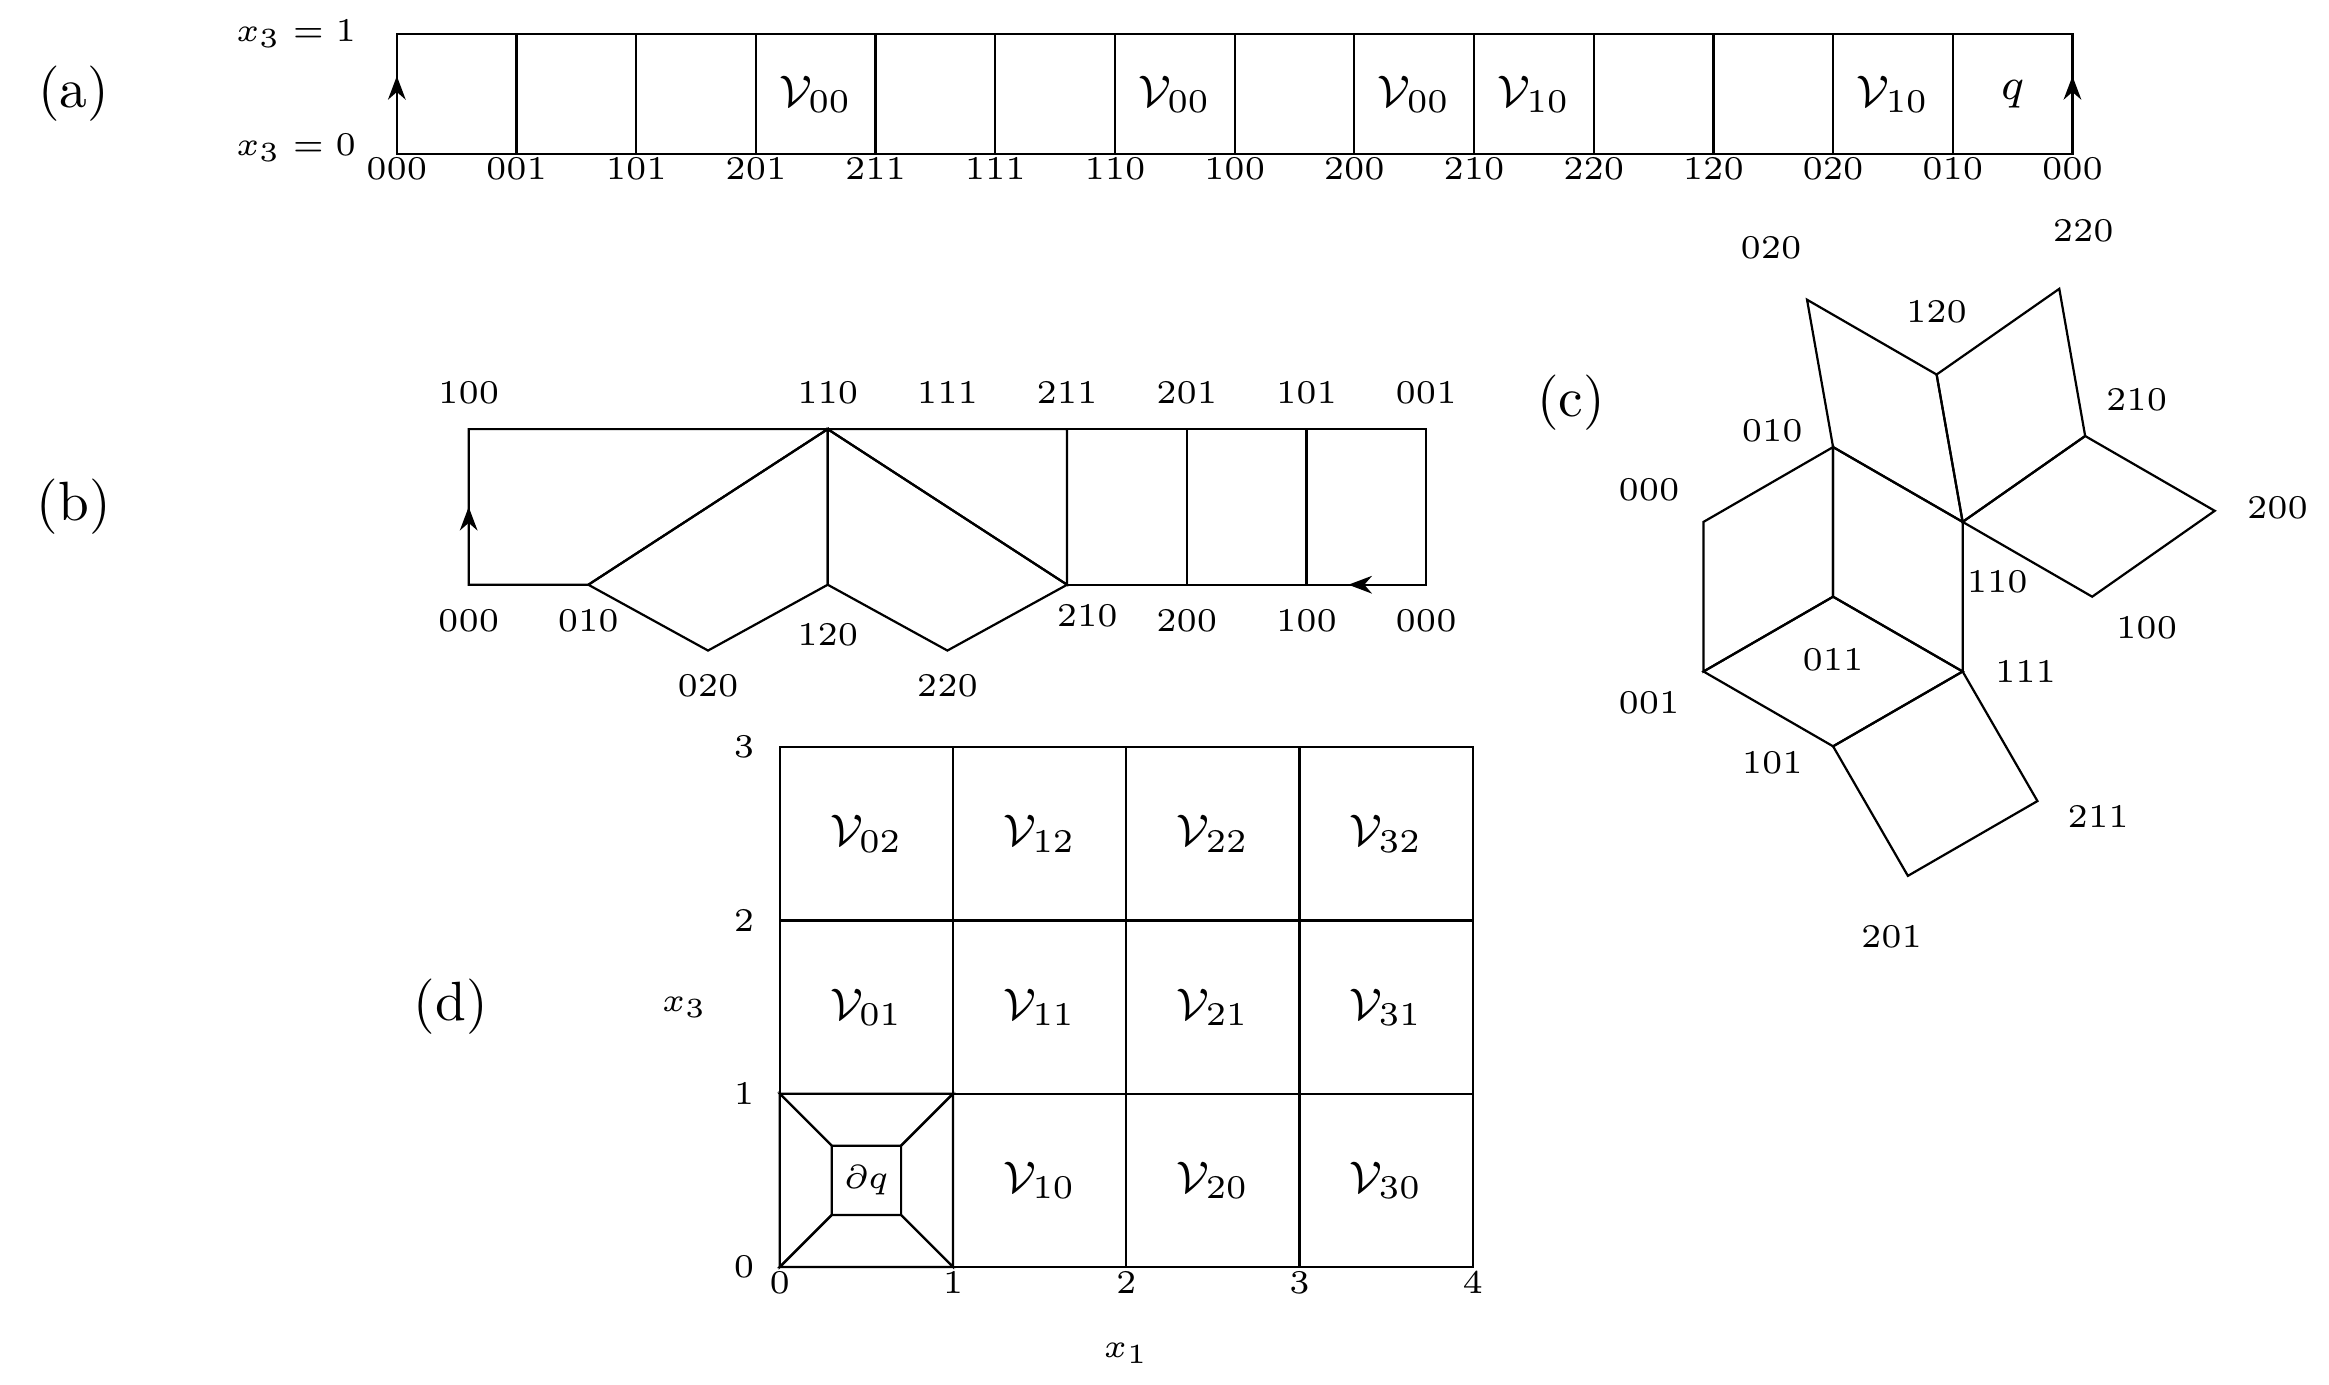
\includegraphics[width=419.1bp]{figures/fig17.png}
\caption{Nets of the surfaces of \cref{thm:surfaces}. Vertex labels in (a)--(c) are $x_0x_1x_2$; edges with equal end labels are identified, and arrows mark the two copies of a cut link. (a)~The cylinder $Y$ between the loop $\gamma$ ($x_3=0$) and $\gamma+\hat3$ ($x_3=1$); the vertex above $x_0x_1x_2$ is $x_0x_1x_21$. (b)~The band $M$ in the slice $x_3=0$; its end links are glued with a half twist. (c)~The cap $K$ in the slice $x_3=1$. Together (a)--(c) form $S$, a lattice $\mathbb{R}P^2$. (d)~The part of $S'$ outside $S\setminus\{q\}$, at $x_0=3$, $x_2=0$: the cell with lower left corner $(x_1,x_3)=(\alpha,\beta)$ is the plaquette $(3\alpha0\beta;13)$ of the torus, and opposite sides of the grid are identified ($x_1$ modulo $4$, $x_3$ modulo $3$); the cell $(0,0)$ is replaced by the tube $T$, whose inner square is glued to the boundary of $q$. A square marked $\mathcal{V}_{\alpha\beta}$ lies in the stack $\mathcal{V}(\alpha,\beta)$; $q=(0000;13)$ lies in $\mathcal{V}(0,0)$ and is absent from $S'$.}
\label{fig:surfaces}
\end{figure}

Plaquettes are written $(x_0x_1x_2x_3;\mu\nu)$. The surface $S\subset\Z^4$ consists of $28$ plaquettes in three groups: a band $M$ in the slice $x_3=0$, a cylinder $Y$ formed by the plaquettes containing direction $3$, and a cap $K$ in the slice $x_3=1$. The plaquettes of $M$ and of $Y$ are listed in cyclic order:
\begin{equation}\label{eq:surface-S}
\begin{aligned}
M:\ &(0000;01),\ (0100;01),\ (1100;01),\ (1100;02),\\
    &(2000;12),\ (1000;02),\ (0000;02);\\
Y:\ &(0000;13),\ (0000;23),\ (0010;03),\ (1010;03),\ (2010;13),\\
    &(1110;03),\ (1100;23),\ (1000;13),\ (1000;03),\ (2000;13),\\
    &(2100;13),\ (1200;03),\ (0200;03),\ (0100;13);\\
K:\ &(0001;12),\ (0011;01),\ (0101;02),\ (0101;01),\\
    &(1101;01),\ (1001;01),\ (1011;01).
\end{aligned}
\end{equation}
The surface $S'$ lies on the periodic lattice $L=(\Z/4\Z)^3\times\Z/3\Z$, with sides $4,4,4,3$ in the directions $0,1,2,3$:
\begin{equation}\label{eq:surface-Sprime}
\begin{aligned}
S'&=\bigl(S\setminus\{q\}\bigr)\cup T\cup Q,\qquad q=(0000;13),\\
T&=\{(3000;01),\ (3000;03),\ (3001;01),\ (3100;03)\},\\
Q&=\{(3\alpha0\beta;13):\ (\alpha,\beta)\in\Z/4\Z\times\Z/3\Z,\ (\alpha,\beta)\ne(0,0)\}.
\end{aligned}
\end{equation}
For $(\alpha,\beta)\in\Z/4\Z\times\Z/3\Z$ the \emph{stack} $\mathcal{V}(\alpha,\beta)=\{(x;13)\in L:x_1=\alpha,\ x_3=\beta\}$ consists of the $16$ plaquettes of the $(1,3)$-planes at these values of $x_1$ and $x_3$.

\begin{theorem}\label{thm:surfaces}
\begin{enumerate}[label=\textup{(\alph*)},leftmargin=*]
\item $S$ is closed and link-connected, $(F,E,\hat V,\chi)=(28,56,29,1)$, and
\[
\int\prod_{p\in S}\Tr U_p\prod_\ell\dd U_\ell=-2^{-27},\qquad\text{hence } s(S)=-1.
\]
Since the vertices of $S$ lie in $\{0,1,2\}^2\times\{0,1\}^2$, reduction to a periodic box with all sides at least $3$ is injective on them, and there links and plaquettes are determined by their vertices. Hence the image of $S$ in such a box is closed and link-connected, with the same $(F,E,\hat V,\chi)$ and the same integral.
\item $S'$ is closed and link-connected on $L$, $(F,E,\hat V,\chi)=(42,84,41,-1)$, and
\[
\int\prod_{p\in S'}\Tr U_p\prod_\ell\dd U_\ell=-2^{-43},\qquad\text{hence } s(S')=-1.
\]
For every $(\alpha,\beta)\in\Z/4\Z\times\Z/3\Z$ the stack $\mathcal{V}(\alpha,\beta)$ meets $S'$ in an odd number of plaquettes.
\end{enumerate}
\end{theorem}

\begin{proof}
\emph{The surface $S$.} Consecutive plaquettes of $M$ in \eqref{eq:surface-S}, the last followed by the first, share exactly one link, and no other two plaquettes of $M$ share a link. The remaining $14$ links of $M$, each in exactly one plaquette of $M$, form the closed loop $\gamma$ through
\[
0000,\ 0010,\ 1010,\ 2010,\ 2110,\ 1110,\ 1100,\ 1000,\ 2000,\ 2100,\ 2200,\ 1200,\ 0200,\ 0100.
\]
The plaquettes of $Y$ are the $14$ plaquettes spanned by a link of $\gamma$ and direction $3$, listed along $\gamma$; consecutive ones share the link in direction $3$ at their common vertex of $\gamma$. The links of $K$ are the $14$ links of $\gamma+\hat3$, each in exactly one plaquette of $K$, and $7$ further links, each in exactly two plaquettes of $K$; three of these meet at $0111$, the only vertex of $K$ off $\gamma+\hat3$. Hence every link of $S$ lies in exactly two plaquettes, $S$ is link-connected, and $E=7+14+14+14+7=56$. The lattice vertices of $S$ are the $14$ vertices of $\gamma$, the $14$ vertices of $\gamma+\hat3$, and $0111$ (\cref{fig:surfaces}); at each of them the corners form a single cycle. Indeed, two plaquettes of $M$ share a link only if they are cyclic neighbours, and the seven shared links have no common endpoint, so at any vertex $x$ the corners of $M$, joined when they share a link, form disjoint chains; an end of a chain contains a link at $x$ lying in only one plaquette of $M$, that is, a link of $\gamma$. If $x$ is a vertex of $\gamma$, then $\gamma$ passes through $x$ once and has two links at $x$, so the corners of $M$ at $x$ form a single chain from one of these links to the other. The only other corners at $x$ are those of the two plaquettes of $Y$ over these two links; they share the link from $x$ to $x+\hat3$ and close the chain to one cycle. The same argument applies at the vertices of $\gamma+\hat3$ with $K$ in place of $M$: the adjacency graph of $K$ is connected, with seven plaquettes and seven shared links, so it has exactly one cycle, formed by $(0001;12)$, $(0011;01)$, $(0101;02)$; the three links they share meet only at $0111$, so at a vertex of $\gamma+\hat3$ the corners of $K$ again form chains, and there is one chain, closed by the two corners of $Y$. At $0111$ the only corners are those of these three plaquettes of $K$, and they form one cycle. Thus $\hat V=29$ and $\chi(S)=29-56+28=1$. If the plaquettes of $M$ are oriented one after the other so that each of the first six shared links is traversed in opposite directions by its two plaquettes, the link shared by the last and the first plaquette is traversed in the same direction by both: $M$ is a M\"obius band, $Y\cup K$ is a disc bounded by $\gamma$, and $S$ is a lattice projective plane.

\emph{The surface $S'$.} On $L$ the vertices of $S$ keep distinct images, so $S\setminus\{q\}$ has the incidences of $S$, except that the four links of the boundary loop $0000,0100,0101,0001$ of $q$ now lie in one plaquette each. The set $Q$ is the torus of the $12$ plaquettes $(3\alpha0\beta;13)$ less $q'=(3000;13)$; its $24$ links lie in two plaquettes of $Q$ each, except the four links of the boundary loop $3000,3100,3101,3001$ of $q'$, which lie in one. Since direction $0$ has period $4$, the four plaquettes of $T$ form a tube joining the loop of $q'$ to the loop of $q$ through the four links in direction $0$ from $x_0=3$ to $x_0=4\equiv0$; each of these links lies in two plaquettes of $T$, and each link of the two loops in one. Hence $S'$ is closed and link-connected, with $F=27+4+11=42$ and $E=56+24+4=84$. Its lattice vertices are the $29$ vertices of $S$ and the $12$ vertices $3\alpha0\beta$ of the torus, and at each of them the corners form a single cycle. At a vertex of $S$ off the loop of $q$ the corners are those of $S$. At a vertex $v$ of the loop of $q$, deleting the corner of $q$ from the cycle of $S$ at $v$ leaves a chain whose ends contain the two links of the loop at $v$; the two plaquettes of $T$ at $v$ give two corners that share the link in direction $0$ at $v$ and contain these two links, so they close the chain. At a vertex of the loop of $q'$ the four plaquettes of the torus around it form one cycle of corners; deleting $q'$ leaves a chain, closed in the same way by the two corners of $T$. At each of the other eight vertices of the torus the corners are those of the four plaquettes of $Q$ around it, which form one cycle. So $\hat V=41$ and $\chi(S')=41-84+42=-1$. The plaquettes of $S'$ in the $(1,3)$-planes are $(0100;13)$, $(1000;13)$, $(2000;13)$, $(2010;13)$, $(2100;13)$ and the eleven plaquettes of $Q$. Thus $\mathcal V(0,0)\cap S'=\{(1000;13),(2000;13),(2010;13)\}$ and $\mathcal V(1,0)\cap S'=\{(0100;13),(2100;13),(3100;13)\}$ have three elements, and each of the other ten stacks meets $S'$ only in its plaquette of $Q$.

\emph{The moments.} By \eqref{eq:crosscap-sign} at $j=\frac12$ and the counts above, $I_S(\frac12)=(-1)^{1}\,2^{29-56}=-2^{-27}$ and $I_{S'}(\frac12)=(-1)^{-1}\,2^{41-84}=-2^{-43}$, and $s(S)=s(S')=-1$. Both values also result, without the use of \eqref{eq:crosscap-sign}, from carrying out the elimination of the proof of \cref{thm:surface-integral} in exact rational arithmetic (\cref{app:verification}).
\end{proof}
\section{Morse--Bott computation for twisted-flat $\mathrm{SU}(2)$ connections}\label{app:morse-bott}

This appendix proves the estimate on which \cref{prop:flux-saturation} rests: on a fixed four-dimensional torus every twisted partition function of the $\SU(2)$ Wilson theory is at most $C_\Lambda\betaW^{-3/2}$ times the untwisted one. As $\betaW\to\infty$ both integrals concentrate on the zero sets of the normalised actions. The untwisted zero set contains a smooth family of abelian flat connections of dimension $3\abs\Lambda+3$ (\cref{lem:mb-lower}); a twisted zero set is a finite union of gauge orbits of dimension $3\abs\Lambda$ and a nondegenerate critical manifold in the sense of Bott \cite{bott1954} (\cref{lem:mb-upper}), because the groups $H^0$ and $H^1$ of the deformation complex of a twisted-flat connection vanish (\cref{lem:mb-H0,lem:mb-H1}). Gaussian integration over the normal directions bounds the untwisted integral from below by a multiple of $\betaW^{-(9\abs\Lambda-3)/2}$ and each twisted integral from above by a multiple of $\betaW^{-9\abs\Lambda/2}$, so $Z(k)/Z\le C_\Lambda\betaW^{-3/2}$ (\cref{prop:mb-ratio}).

\subsection{Setting}
Let $\Lambda=(\Z/n_0\Z)\times(\Z/n_1\Z)\times(\Z/n_2\Z)\times(\Z/n_3\Z)$ with all $n_\mu\ge2$; direction $0$ is time, $n_0=T$, and $s=(n_1,n_2,n_3)$ is the spatial torus. As in \cref{sec:necessary} we also write $\Lambda=s\times(\Z/T\Z)$; the order of the factors is immaterial, and the time axis is the axis labelled $4$ in \cref{sec:centre}. Write $e_\mu$ for the unit vectors, $E$ for the set of links $(x,\mu)$ and $P$ for the set of plaquettes $p=(x;\mu,\nu)$ with $0\le\mu<\nu\le3$, so that $\abs E=4\abs\Lambda$ and $\abs P=6\abs\Lambda$; a $(j,0)$-plaquette is a plaquette $(x;0,j)$. A configuration is $U=(U_{x,\mu})\in\mathcal C:=\SU(2)^E$, $\dd U$ is the product of the normalised Haar measures, and
\begin{equation}\label{eq:mb-plaquette}
U_p=U_{x,\mu}U_{x+e_\mu,\nu}U_{x+e_\nu,\mu}^{-1}U_{x,\nu}^{-1}\qquad(p=(x;\mu,\nu))
\end{equation}
is the plaquette variable, written $Q_p$ in \eqref{eq:wilson-weight}. On $\mathfrak g=\mathfrak{su}(2)$ we use the inner product $\ip XY=-\frac12\Tr(XY)$. For $X=i(y_1\sigma_1+y_2\sigma_2+y_3\sigma_3)$ one has $X^2=-\abs y^2\mathbf 1$, hence $\abs X=\abs y$, $e^X=\cos\abs X\,\mathbf 1+\abs X^{-1}\sin\abs X\,X$, and
\begin{equation}\label{eq:mb-cos}
1-\tfrac12\Tr e^X=1-\cos\abs X\qquad(X\in\mathfrak g).
\end{equation}
In particular $\frac12\Tr u\le1$ for $u\in\SU(2)$, with equality only at $u=\mathbf 1$. The adjoint representation maps $\SU(2)$ onto $\mathrm{SO}(\mathfrak g)$ with kernel $\{\pm\mathbf 1\}$. The spaces $\mathfrak g^\Lambda$, $\mathfrak g^E$, $\mathfrak g^P$ carry the sum inner products. The gauge group $\mathcal G=\SU(2)^\Lambda$ acts by $(g\cdot U)_{x,\mu}=g_xU_{x,\mu}g_{x+e_\mu}^{-1}$, so that $(g\cdot U)_p=g_xU_pg_x^{-1}$; the action preserves $\dd U$, because it multiplies each link variable on the left and on the right by fixed elements.

\emph{The deformation complex.} For $\gamma=(\gamma_{x,\mu})\in\mathrm{SO}(\mathfrak g)^E$ define $\gamma_p$ by \eqref{eq:mb-plaquette} and linear maps $\delta^0_\gamma\colon\mathfrak g^\Lambda\to\mathfrak g^E$, $\delta^1_\gamma\colon\mathfrak g^E\to\mathfrak g^P$ by
\begin{equation}\label{eq:mb-complex}
\begin{aligned}
(\delta^0_\gamma\xi)_{x,\mu}&=\xi_x-\gamma_{x,\mu}\xi_{x+e_\mu},\\
(\delta^1_\gamma X)_{(x;\mu,\nu)}&=X_{x,\mu}+\gamma_{x,\mu}X_{x+e_\mu,\nu}-\gamma_{x,\nu}X_{x+e_\nu,\mu}-X_{x,\nu}.
\end{aligned}
\end{equation}
Call $\gamma$ flat if $\gamma_p=1$ for all $p$, that is, $\gamma_{x,\mu}\gamma_{x+e_\mu,\nu}=\gamma_{x,\nu}\gamma_{x+e_\nu,\mu}$. Substituting $X=\delta^0_\gamma\xi$ in \eqref{eq:mb-complex} gives $(\delta^1_\gamma\delta^0_\gamma\xi)_{(x;\mu,\nu)}=(\gamma_{x,\nu}\gamma_{x+e_\nu,\mu}-\gamma_{x,\mu}\gamma_{x+e_\mu,\nu})\xi_{x+e_\mu+e_\nu}$, so
\begin{equation}\label{eq:mb-dd}
\delta^1_\gamma\delta^0_\gamma=0\qquad\text{if $\gamma$ is flat.}
\end{equation}
For $\kappa\in\mathrm{SO}(\mathfrak g)^\Lambda$ put $\gamma^\kappa_{x,\mu}=\kappa_x\gamma_{x,\mu}\kappa_{x+e_\mu}^{-1}$, and let $\kappa$ act on $\mathfrak g^\Lambda$, $\mathfrak g^E$, $\mathfrak g^P$ by applying $\kappa_x$ to the component at $x$, at $(x,\mu)$ and at $(x;\mu,\nu)$. Then $\gamma^\kappa_p=\kappa_x\gamma_p\kappa_x^{-1}$ for $p=(x;\mu,\nu)$, and directly from \eqref{eq:mb-complex}
\begin{equation}\label{eq:mb-covariance}
\delta^i_{\gamma^\kappa}\circ\kappa=\kappa\circ\delta^i_\gamma\qquad(i=0,1),
\end{equation}
so $\kappa$ maps $\ker\delta^i_\gamma$ and $\operatorname{im}\delta^i_\gamma$ onto $\ker\delta^i_{\gamma^\kappa}$ and $\operatorname{im}\delta^i_{\gamma^\kappa}$. For $U\in\mathcal C$ write $\delta^i_U=\delta^i_{\operatorname{Ad}U}$, where $(\operatorname{Ad}U)_{x,\mu}=\operatorname{Ad}(U_{x,\mu})$. Then $\operatorname{Ad}(g\cdot U)=(\operatorname{Ad}U)^{\operatorname{Ad}g}$ for $g\in\mathcal G$, and differentiating $g_xU_{x,\mu}g_{x+e_\mu}^{-1}$ gives, for $\xi\in\mathfrak g^\Lambda$,
\begin{equation}\label{eq:mb-orbit}
\frac{\mathrm d}{\mathrm dt}\Big|_{t=0}\bigl(e^{t\xi}\cdot U\bigr)_{x,\mu}=(\delta^0_U\xi)_{x,\mu}\,U_{x,\mu}.
\end{equation}

\emph{Twisted actions.} Fix $k\in\{0,1\}^3$, and put $\eta_p=-1$ if $p=(x;0,j)$ with $k_j=1$, $x_j=n_j-1$ and $x_0=n_0-1$, and $\eta_p=1$ otherwise. For each $j$ with $k_j=1$ the plaquettes with $\eta_p=-1$ form a stack $\Sigma_j$ of $(j,0)$-plaquettes, which meets every $(j,0)$ coordinate $2$-torus $\{y+ae_j+be_0\}$ of $\Lambda$ in exactly one plaquette. For $G=\SU(2)$ the Wilson weight \eqref{eq:wilson-weight} is $\exp(2\beta\sum_p\Tr U_p)=\exp(\betaW\sum_p\frac12\Tr U_p)$, with $\betaW=4\beta$. Let $Z(k)$ be the integral of $\exp(\betaW\sum_p\frac12\eta'_p\Tr U_p)\dd U$, where $\eta'_p=-1$ exactly on the stack of $(j,0)$-plaquettes with $x_j=0$ and $x_0=n_0-1$ for each $j$ with $k_j=1$, and $\eta'_p=1$ on all other plaquettes; and $Z=Z(0)$. For $T\ge3$, \cref{lem:centre-operators}\textup{(c)} states that $Z(k)=\Tr(z^k\TT_s^T)$, with one and the same normalisation for every $k$, including $k=0$; the plaquettes of that lemma carry the opposite orientation, which does not change the weight, because $\Tr u^{-1}=\Tr u$ on $\SU(2)$. For $T=2$ we take the integral as the definition of $Z(k)$. Multiplying by $-\mathbf 1$ the links $(y,j)$ (resp.\ $(y,0)$) with $y_j=a$, $y_0=b$ preserves $\dd U$ and changes the sign of $U_p$ exactly for the $(j,0)$-plaquettes with $x_j=a$, $x_0\in\{b-1,b\}$ (resp.\ $x_j\in\{a-1,a\}$, $x_0=b$), since every other plaquette contains two or none of these links; so it moves a stack from $(x_j,x_0)=(a,b-1)$ (resp.\ $(a-1,b)$) to $(a,b)$, and we may take $\eta'=\eta$. With the normalised actions
\begin{equation}\label{eq:mb-actions}
S(U)=\sum_{p\in P}\bigl(1-\tfrac12\Tr U_p\bigr),\qquad S^k(U)=\sum_{p\in P}\bigl(1-\tfrac12\eta_p\Tr U_p\bigr),
\end{equation}
which are nonnegative and gauge invariant, $Z(k)=e^{\betaW\abs P}\int_{\mathcal C}e^{-\betaW S^k(U)}\dd U$ for every $k$, the factor $e^{\betaW\abs P}$ cancels, and
\begin{equation}\label{eq:mb-ratio-integrals}
\frac{Z(k)}{Z}=\frac{\int_{\mathcal C}e^{-\betaW S^k(U)}\dd U}{\int_{\mathcal C}e^{-\betaW S(U)}\dd U}.
\end{equation}

\subsection{Abelian flat connections and the lower bound}

\begin{lemma}\label{lem:mb-lower}
There is $c_1>0$, depending only on $\Lambda$, such that $\int_{\mathcal C}e^{-\lambda S}\dd U\ge c_1\lambda^{-(9\abs\Lambda-3)/2}$ for every $\lambda\ge1$.
\end{lemma}

\begin{proof}
For $\theta\in(0,\pi)^4$ let $A(\theta)_{x,\mu}=\exp(i\theta_\mu\sigma_3/n_\mu)$. These elements commute and $A(\theta)_{x,\mu}$ depends only on $\mu$, so $A(\theta)_p=\mathbf 1$ for every $p$, and $S(g\cdot A(\theta))=0$ for every $g\in\mathcal G$. Let $\mathfrak m=\operatorname{span}\{i\sigma_1,i\sigma_2\}$, fix a site $o$, and let
\[
\mathcal D=\bigl\{(g,\theta)\in\mathcal G\times(0,\pi)^4:\ g_o=e^Y\ \text{for some }Y\in\mathfrak m\text{ with }\abs Y<1\bigr\}.
\]
Since the exponential map is a diffeomorphism from $\{Y\in\mathfrak g:\abs Y<\pi\}$ onto $\SU(2)\setminus\{-\mathbf 1\}$, $\mathcal D$ is a submanifold of dimension $N_{\mathcal D}:=3(\abs\Lambda-1)+2+4=3\abs\Lambda+3$. Put $\Phi(g,\theta)=g\cdot A(\theta)$, fix $\theta\in(0,\pi)^4$ and write $A=A(\theta)$. A tangent vector to $\mathcal D$ at $(\mathbf 1,\theta)$ is a pair $(\xi,\dot\theta)$ with $\xi\in\mathfrak g^\Lambda$, $\xi_o\in\mathfrak m$, $\dot\theta\in\R^4$, and by \eqref{eq:mb-orbit}
\[
\bigl(\mathrm d\Phi(\xi,\dot\theta)\bigr)_{x,\mu}A_{x,\mu}^{-1}=\xi_x-\operatorname{Ad}(A_{x,\mu})\xi_{x+e_\mu}+i\dot\theta_\mu\sigma_3/n_\mu .
\]
Suppose that this vanishes for all $(x,\mu)$, and write $\xi_x=\alpha_x\,i\sigma_3+\xi^\perp_x$ with $\alpha_x\in\R$, $\xi^\perp_x\in\mathfrak m$. The map $\operatorname{Ad}(e^{i\varphi\sigma_3})$ fixes $i\sigma_3$ and rotates $\mathfrak m$ by the angle $2\varphi$. The $i\sigma_3$-component gives $\alpha_x-\alpha_{x+e_\mu}+\dot\theta_\mu/n_\mu=0$; summing over the $n_\mu$ sites of a line in direction $\mu$ gives $\dot\theta_\mu=0$, and then $\alpha$ is constant. The $\mathfrak m$-component gives $\xi^\perp_x=\operatorname{Ad}(A_{x,\mu})\xi^\perp_{x+e_\mu}$; applying this $n_\mu$ times along a line gives $\xi^\perp_x=\operatorname{Ad}(e^{i\theta_\mu\sigma_3})\xi^\perp_x$, a rotation by $2\theta_\mu\in(0,2\pi)$, so $\xi^\perp=0$. Hence $\xi=\alpha\,i\sigma_3$ with $\alpha$ constant, and $\xi_o\in\mathfrak m$ forces $\alpha=0$. So $\Phi$ is an immersion at $(\mathbf 1,\theta)$.

By the immersion theorem there are a chart $\chi$ of $\mathcal C$ at $A$ and $\delta\in(0,1]$ such that, with $N_E:=3\abs E=12\abs\Lambda$, the image of $\chi$ contains $K=\bar B^{N_{\mathcal D}}_\delta\times\bar B^{N_E-N_{\mathcal D}}_\delta\subset\R^{N_{\mathcal D}}\times\R^{N_E-N_{\mathcal D}}$ and $\chi^{-1}(y,0)\in\Phi(\mathcal D)$ for $\abs y\le\delta$. On $K$ let $f=S\circ\chi^{-1}$, and let $\rho$ be the density of the image of $\dd U$ under $\chi$, which is smooth and positive; let $\rho_0>0$ be the minimum of $\rho$ and $M$ the maximum of the norm of $\partial_z^2f$ on $K$. Since $f\ge0$ and $f(y,0)=0$, also $\partial_zf(y,0)=0$, and Taylor's formula in $z$ gives $f(y,z)\le\frac12M\abs z^2$ on $K$. For $\lambda\ge1$, substituting $z=\lambda^{-1/2}w$,
\begin{align*}
\int_{\mathcal C}e^{-\lambda S}\dd U&\ge\rho_0\int_{\abs y\le\delta}\int_{\abs z\le\delta}e^{-\lambda M\abs z^2/2}\dd z\dd y\\
&=\rho_0\abs{B^{N_{\mathcal D}}_\delta}\,\lambda^{-\frac{N_E-N_{\mathcal D}}2}\int_{\abs w\le\delta\sqrt\lambda}e^{-M\abs w^2/2}\dd w\ge c_1\lambda^{-\frac{N_E-N_{\mathcal D}}2},
\end{align*}
with $c_1=\rho_0\abs{B^{N_{\mathcal D}}_\delta}\int_{\abs w\le\delta}e^{-M\abs w^2/2}\dd w$. Finally $N_E-N_{\mathcal D}=9\abs\Lambda-3$.
\end{proof}

\subsection{Twisted-flat connections}
Let $k\ne0$ and $F^k=\{U\in\mathcal C:S^k(U)=0\}$. By \eqref{eq:mb-cos} every summand of $S^k$ is nonnegative and vanishes exactly when $\eta_pU_p=\mathbf 1$, so
\[
F^k=\{U\in\mathcal C:\ U_p=\eta_p\mathbf 1\ \text{for all }p\in P\},
\]
a compact $\mathcal G$-invariant set, whose elements are the twisted-flat connections. For $U\in F^k$ the connection $\operatorname{Ad}U$ is flat, because $\operatorname{Ad}(U_p)=\operatorname{Ad}(\pm\mathbf 1)=1$.

\begin{lemma}\label{lem:mb-nonempty}
Let $U^\sharp_{x,j}=i\sigma_1$ if $k_j=1$ and $x_j=n_j-1$, $U^\sharp_{x,0}=i\sigma_3$ if $x_0=n_0-1$, and $U^\sharp_\ell=\mathbf 1$ on all other links. Then $U^\sharp\in F^k$; in particular $F^k\ne\emptyset$.
\end{lemma}

\begin{proof}
$U^\sharp_{x,\mu}$ depends only on $\mu$ and $x_\mu$. Hence for $p=(x;\mu,\nu)$ one has $U^\sharp_{x+e_\nu,\mu}=U^\sharp_{x,\mu}$ and $U^\sharp_{x+e_\mu,\nu}=U^\sharp_{x,\nu}$, so $U^\sharp_p=aba^{-1}b^{-1}$ with $a=U^\sharp_{x,\mu}$, $b=U^\sharp_{x,\nu}$. If $\mu\ge1$, then $a,b\in\{\mathbf 1,i\sigma_1\}$ commute and $U^\sharp_p=\mathbf 1$. If $\mu=0$ and $\nu=j$, then $a\in\{\mathbf 1,i\sigma_3\}$, $b\in\{\mathbf 1,i\sigma_1\}$, and $U^\sharp_p\ne\mathbf 1$ only if $a=i\sigma_3$ and $b=i\sigma_1$, that is, if $x_0=n_0-1$, $k_j=1$ and $x_j=n_j-1$; then $U^\sharp_p=(i\sigma_3)(i\sigma_1)(i\sigma_3)^{-1}(i\sigma_1)^{-1}=(\sigma_3\sigma_1)^2=(i\sigma_2)^2=-\mathbf 1$. So $U^\sharp_p=\eta_p\mathbf 1$ for every $p$.
\end{proof}

\begin{lemma}\label{lem:mb-hessian}
Let $U\in F^k$ and, for $X\in\mathfrak g^E$, let $(e^XU)_\ell=e^{X_\ell}U_\ell$. Then $\delta^1_U\delta^0_U=0$, and there is $C_U\in(0,\infty)$ such that
\begin{equation}\label{eq:mb-taylor}
\Bigl|S^k(e^XU)-\tfrac12\abs{\delta^1_UX}^2\Bigr|\le C_U\abs X^3\qquad(\abs X\le1).
\end{equation}
\end{lemma}

\begin{proof}
The first claim is \eqref{eq:mb-dd}. Fix $p=(x;\mu,\nu)$, put $a=U_{x,\mu}$, $b=U_{x+e_\mu,\nu}$, $c=U_{x+e_\nu,\mu}$, $d=U_{x,\nu}$, and write $X_1,X_2,X_3,X_4$ for the corresponding components of $X$. Moving the exponentials to the left with $ue^Yu^{-1}=e^{\operatorname{Ad}(u)Y}$ gives
\[
(e^XU)_p=e^{X_1}e^{\operatorname{Ad}(a)X_2}e^{-\operatorname{Ad}(abc^{-1})X_3}e^{-\operatorname{Ad}(U_p)X_4}U_p .
\]
Since $U_p=\eta_p\mathbf 1$ is central, $\operatorname{Ad}(U_p)=1$ and $\operatorname{Ad}(abc^{-1})=\operatorname{Ad}(U_pd)=\operatorname{Ad}(d)$, so
\begin{equation}\label{eq:mb-product}
\eta_p(e^XU)_p=e^{X_{x,\mu}}\,e^{\operatorname{Ad}(U_{x,\mu})X_{x+e_\mu,\nu}}\,e^{-\operatorname{Ad}(U_{x,\nu})X_{x+e_\nu,\mu}}\,e^{-X_{x,\nu}}.
\end{equation}
Let $f(X)=S^k(e^XU)$; it is smooth, $f\ge0$ and $f(0)=0$. Fix $X$. By \eqref{eq:mb-product}, $t\mapsto\eta_p(e^{tX}U)_p$ is a smooth curve in $\SU(2)$ through $\mathbf 1$ with velocity $(\delta^1_UX)_p$ at $t=0$. The exponential map of $\SU(2)$ is a local diffeomorphism at $0$ with differential the identity, so for small $\abs t$ the curve equals $e^{Z_p(t)}$ with $Z_p$ smooth, $Z_p(0)=0$ and $Z_p'(0)=(\delta^1_UX)_p$. By \eqref{eq:mb-cos}, $f(tX)=\sum_p(1-\cos\abs{Z_p(t)})=\frac12t^2\abs{\delta^1_UX}^2+O(t^3)$. So the first derivative of $f$ at $0$ vanishes and the second is the quadratic form $X\mapsto\abs{\delta^1_UX}^2$, and Taylor's formula, with the third derivatives of $f$ bounded on $\{\abs X\le1\}$, gives \eqref{eq:mb-taylor}.
\end{proof}

\begin{lemma}[$H^0=0$]\label{lem:mb-H0}
For $U\in F^k$, $k\ne0$, one has $\ker\delta^0_U=0$.
\end{lemma}

\begin{proof}
Let $\delta^0_U\xi=0$, that is, $\xi_x=\operatorname{Ad}(U_{x,\mu})\xi_{x+e_\mu}$ for all $(x,\mu)$. Since $\operatorname{Ad}$ is isometric and $\Lambda$ is connected, $\abs{\xi_x}=r$ does not depend on $x$. Suppose $r>0$. As $\mathrm{SO}(\mathfrak g)=\operatorname{Ad}(\SU(2))$ acts transitively on the sphere of radius $r$, there is $g\in\mathcal G$ with $\operatorname{Ad}(g_x)\xi_x=r\,i\sigma_3$ for every $x$. Put $U'=g\cdot U\in F^k$ and $\xi'_x=r\,i\sigma_3$. By \eqref{eq:mb-covariance} with $\kappa=\operatorname{Ad}g$, $\delta^0_{U'}\xi'=0$; so $\operatorname{Ad}(U'_{x,\mu})$ fixes $i\sigma_3$, $U'_{x,\mu}$ commutes with $\sigma_3$, and $U'_{x,\mu}=\exp(i\phi_{x,\mu}\sigma_3)$ with $\phi_{x,\mu}\in\R$. Then $U'_p=\exp(i(\mathrm d\phi)_p\sigma_3)$ with $(\mathrm d\phi)_{(x;\mu,\nu)}=\phi_{x,\mu}+\phi_{x+e_\mu,\nu}-\phi_{x+e_\nu,\mu}-\phi_{x,\nu}$. Choose $j$ with $k_j=1$ and a $(j,0)$ coordinate $2$-torus $\Pi=\{y+ae_j+be_0\}$. In the sum of $(\mathrm d\phi)_{(x;0,j)}$ over the $n_0n_j$ points $x\in\Pi$, the terms $\phi_{x,0}-\phi_{x+e_j,0}$ cancel in the sum over $a$ and the terms $\phi_{x+e_0,j}-\phi_{x,j}$ cancel in the sum over $b$; since the factors commute, $\prod_{x\in\Pi}U'_{(x;0,j)}=\mathbf 1$. On the other hand $U'_p=\eta_p\mathbf 1$, and exactly one plaquette $(x;0,j)$ with $x\in\Pi$ lies in $\Sigma_j$, so the product equals $-\mathbf 1$. This contradiction shows $r=0$.
\end{proof}

\begin{lemma}[$H^1=0$]\label{lem:mb-H1}
For $U\in F^k$, $k\ne0$, one has $\ker\delta^1_U=\operatorname{im}\delta^0_U$. Consequently $\dim\ker\delta^1_U=3\abs\Lambda$ and $\rank\delta^1_U=9\abs\Lambda$.
\end{lemma}

\begin{proof}
Let $\gamma=\operatorname{Ad}U$; it is flat.

\emph{Step 1: seam gauge.} Let $B_0=\prod_\mu\{0,\dots,n_\mu-1\}\subset\Z^4$, identified with $\Lambda$ by reduction modulo $(n_0,\dots,n_3)$. A link $(x,\mu)$, $x\in B_0$, is \emph{interior} if $x_\mu\le n_\mu-2$ and a \emph{seam} link if $x_\mu=n_\mu-1$. An edge path in $B_0$ uses only interior links; its transport is the ordered product of $\gamma_{x,\mu}$ over its steps $x\to x+e_\mu$ and of $\gamma_{x,\mu}^{-1}$ over its steps $x+e_\mu\to x$. Two consecutive steps $y\to y+\epsilon e_\mu\to y+\epsilon e_\mu+\epsilon'e_\nu$ ($\mu\ne\nu$, $\epsilon,\epsilon'\in\{\pm1\}$) can be replaced by $y\to y+\epsilon'e_\nu\to y+\epsilon e_\mu+\epsilon'e_\nu$, whose middle vertex again lies in $B_0$; the transport does not change, because the four vertices span a plaquette $p$ with $\gamma_p=1$. Deleting two consecutive opposite steps does not change it either. Using the first replacement to sort the steps by direction (each transposition keeps the path in $B_0$), and then deleting consecutive opposite steps, turns every edge path in $B_0$ from $0$ to $x$ into the path that runs monotonically in direction $0$, then $1$, $2$, $3$. So the transport $\kappa_x$ from $0$ to $x$ does not depend on the path, $\kappa_{x+e_\mu}=\kappa_x\gamma_{x,\mu}$ for every interior link, and $\gamma':=\gamma^\kappa$ equals $1$ on all interior links. For a seam link put $h_\mu(x)=\gamma'_{x,\mu}$. If $x_\mu=n_\mu-1$ and $x_\nu\le n_\nu-2$, the plaquette spanned at $x$ by $e_\mu$ and $e_\nu$ has the interior links $(x+e_\mu,\nu)$, $(x,\nu)$ and the seam links $(x,\mu)$, $(x+e_\nu,\mu)$, and flatness gives $h_\mu(x)=h_\mu(x+e_\nu)$; so $h_\mu(x)=:h_\mu$ does not depend on $x$. If $x_\mu=n_\mu-1$ and $x_\nu=n_\nu-1$, all four links are seam links and flatness gives $h_\mu h_\nu=h_\nu h_\mu$. Thus $h_0,\dots,h_3\in\mathrm{SO}(\mathfrak g)$ commute. By \eqref{eq:mb-covariance} it suffices to prove the lemma for $\gamma'$.

\emph{Step 2: unfolding.} Because the $h_\mu$ commute, every $\xi\in\mathfrak g^\Lambda$ extends uniquely to a map $f\colon\Z^4\to\mathfrak g$ with $f|_{B_0}=\xi$ and $f(y+n_\mu e_\mu)=h_\mu f(y)$ for all $y$ and $\mu$. Likewise $X\in\mathfrak g^E$ and $Y\in\mathfrak g^P$ give quasi-periodic families $(F_\mu)$ and $(F_{\mu\nu})_{\mu<\nu}$ with $F_\mu(x)=X_{x,\mu}$ and $F_{\mu\nu}(x)=Y_{(x;\mu,\nu)}$ for $x\in B_0$. In these terms
\begin{equation}\label{eq:mb-unfolded}
(\delta^0_{\gamma'}\xi)_\mu(x)=f(x)-f(x+e_\mu),\qquad(\delta^1_{\gamma'}X)_{\mu\nu}(x)=F_\mu(x)+F_\nu(x+e_\mu)-F_\mu(x+e_\nu)-F_\nu(x)
\end{equation}
for all $x\in\Z^4$. Indeed both sides are quasi-periodic, and for $x\in B_0$ \eqref{eq:mb-unfolded} is \eqref{eq:mb-complex}: $\gamma'_{x,\mu}=1$ on interior links, and on a seam link $h_\mu$ applied to the value at $x+e_\mu-n_\mu e_\mu$ is the value at $x+e_\mu$.

\emph{Step 3: Fourier modes.} Complexify. The commuting orthogonal maps $h_\mu$ are simultaneously unitarily diagonalisable on $\mathfrak g\otimes\C\cong\C^3$: there are orthogonal lines $\ell_1,\ell_2,\ell_3$ with $h_\mu=e^{i\vartheta_{\tau,\mu}}$ on $\ell_\tau$, $\vartheta_{\tau,\mu}\in\R$. For $w_\tau\in\ell_\tau\setminus\{0\}$, the quasi-periodic maps $\Z^4\to\ell_\tau$ form a space of dimension $\abs\Lambda$, as they are determined by their values on $B_0$. It contains the $\abs\Lambda$ maps $x\mapsto e^{iq\cdot x}w_\tau$ with $q\in\Theta_\tau=\{q:\ q_\mu=(\vartheta_{\tau,\mu}+2\pi r_\mu)/n_\mu,\ 0\le r_\mu<n_\mu\}$, which are linearly independent as distinct characters of $\Z^4$; so they form a basis. Hence, in each degree, the complexification of \eqref{eq:mb-unfolded} is the direct sum over $\tau$ and $q\in\Theta_\tau$ of the subcomplexes formed by $e^{iq\cdot x}w_\tau$ times constant vectors in $\C$, $\C^4$, $\C^6$, and on such a summand, with $v_\mu=e^{iq_\mu}-1$, it reads
\begin{equation}\label{eq:mb-koszul}
\C\longrightarrow\C^4\longrightarrow\C^6,\qquad c\longmapsto-c\,v,\qquad(a_\mu)\longmapsto(v_\mu a_\nu-v_\nu a_\mu)_{\mu<\nu}.
\end{equation}
This is a Koszul complex. If $v\ne0$, it is exact at $\C^4$: if $v_\mu a_\nu=v_\nu a_\mu$ for all $\mu,\nu$ and $v_{\mu_0}\ne0$, then $a=(a_{\mu_0}/v_{\mu_0})v$ is the image of $-a_{\mu_0}/v_{\mu_0}$. If $v=0$, then $e^{i\vartheta_{\tau,\mu}}=e^{in_\mu q_\mu}=1$ for every $\mu$, so the $h_\mu$ have a common fixed vector in $\C^3$; being real, they have a common fixed vector $w\in\mathfrak g\setminus\{0\}$. The constant map $f\equiv w$ is quasi-periodic, and $\delta^0_{\gamma'}f=0$ by \eqref{eq:mb-unfolded}; by \eqref{eq:mb-covariance}, $\ker\delta^0_U\ne0$, contrary to \cref{lem:mb-H0}. So $v\ne0$ on every summand, and the complexified complex is exact at $(\mathfrak g\otimes\C)^E$. As $\delta^0_{\gamma'}$ and $\delta^1_{\gamma'}$ are real, $\ker\delta^1_{\gamma'}=\operatorname{im}\delta^0_{\gamma'}$. The dimension count follows from the injectivity of $\delta^0_U$ (\cref{lem:mb-H0}) and $\dim\mathfrak g^E=12\abs\Lambda$.
\end{proof}

\subsection{The Morse--Bott upper bound}

\begin{lemma}\label{lem:mb-upper}
Let $k\ne0$.
\begin{enumerate}[label=\textup{(\roman*)},leftmargin=*]
\item $F^k$ is the disjoint union of finitely many $\mathcal G$-orbits. Each orbit $\mathcal G\cdot U$ is a compact embedded submanifold of $\mathcal C$ of dimension $3\abs\Lambda$, with tangent space $\{(X_\ell U_\ell)_\ell:X\in\operatorname{im}\delta^0_U\}$ at $U$, and the quadratic form $X\mapsto\abs{\delta^1_UX}^2$ of \cref{lem:mb-hessian} is positive definite on the normal space $\mathfrak n_U:=(\operatorname{im}\delta^0_U)^\perp\subset\mathfrak g^E$, which has dimension $9\abs\Lambda$.
\item There is $C_2<\infty$, depending only on $\Lambda$ and $k$, such that $\int_{\mathcal C}e^{-\lambda S^k}\dd U\le C_2\lambda^{-9\abs\Lambda/2}$ for every $\lambda>0$.
\end{enumerate}
\end{lemma}

\begin{proof}
Let $U\in F^k$. By \eqref{eq:mb-orbit} the Lie algebra of the stabiliser of $U$ in $\mathcal G$ lies in $\ker\delta^0_U=0$ (\cref{lem:mb-H0}). So the stabiliser is finite, the orbit map is an immersion at every point, and $\mathcal G\cdot U$ is a compact embedded submanifold of dimension $\dim\mathcal G=3\abs\Lambda$ with the stated tangent space. By \cref{lem:mb-H1}, $\mathfrak n_U=(\ker\delta^1_U)^\perp$ has dimension $12\abs\Lambda-3\abs\Lambda$, and $\delta^1_U$ is injective on it; hence $\abs{\delta^1_UX}^2\ge\mu_U\abs X^2$ on $\mathfrak n_U$ for some $\mu_U>0$. This proves the statements of (i) about a single orbit. By \eqref{eq:mb-taylor},
\begin{equation}\label{eq:mb-quadratic}
S^k(e^XU)\ge\tfrac14\mu_U\abs X^2\qquad\bigl(X\in\mathfrak n_U,\ \abs X\le\varepsilon_U\bigr),\qquad\varepsilon_U:=\min\{1,\mu_U/(4C_U)\}.
\end{equation}
Let $\Psi_U\colon\mathcal G\times\mathfrak n_U\to\mathcal C$, $\Psi_U(g,X)=g\cdot(e^XU)$. By \eqref{eq:mb-orbit}, its differential at $(\mathbf 1,0)$ is $(\xi,X)\mapsto((\delta^0_U\xi+X)_\ell U_\ell)_\ell$, which is bijective because $\delta^0_U$ is injective and $\mathfrak g^E=\operatorname{im}\delta^0_U\oplus\mathfrak n_U$. By the inverse function theorem there are an open neighbourhood $O$ of $\mathbf 1$ in $\mathcal G$ and $\varepsilon\in(0,\varepsilon_U]$ such that $\Psi_U$ maps a neighbourhood of $\bar O\times\bar B_\varepsilon$, where $B_\varepsilon=\{X\in\mathfrak n_U:\abs X<\varepsilon\}$, diffeomorphically onto an open set; let $J_U$ bound its Jacobian on $\bar O\times\bar B_\varepsilon$ with respect to $\dd g\,\dd X$, where $\dd g$ is the Haar probability measure and $\dd X$ the Lebesgue measure of $\mathfrak n_U$. Cover $\mathcal G$ by translates $h_1O,\dots,h_qO$. Since $\Psi_U(hg,X)=h\cdot\Psi_U(g,X)$, the set
\[
W_U:=\Psi_U(\mathcal G\times B_\varepsilon)=\bigcup_{i=1}^qh_i\cdot\Psi_U(O\times B_\varepsilon)
\]
is open and contains $\mathcal G\cdot U$. If $\Psi_U(g,X)\in F^k$ with $X\in B_\varepsilon$, then $0=S^k(g\cdot e^XU)=S^k(e^XU)\ge\frac14\mu_U\abs X^2$, so $X=0$; hence $F^k\cap W_U=\mathcal G\cdot U$. Since $S^k$ and $\dd U$ are gauge invariant, the change of variables $u=\Psi_U(g,X)$ on $O\times B_\varepsilon$ and \eqref{eq:mb-quadratic} give, for every $\lambda>0$,
\begin{equation}\label{eq:mb-gaussian}
\int_{W_U}e^{-\lambda S^k}\dd U\le q\int_{\Psi_U(O\times B_\varepsilon)}e^{-\lambda S^k}\dd U\le qJ_U\int_{\mathfrak n_U}e^{-\lambda\mu_U\abs X^2/4}\dd X=qJ_U\Bigl(\frac{4\pi}{\mu_U\lambda}\Bigr)^{9\abs\Lambda/2}.
\end{equation}
The open sets $W_U$, $U\in F^k$, cover the compact set $F^k$; choose $U_1,\dots,U_r$ with $F^k\subset W:=W_{U_1}\cup\dots\cup W_{U_r}$. Then $F^k=\mathcal G\cdot U_1\cup\dots\cup\mathcal G\cdot U_r$, and distinct orbits are disjoint; with \cref{lem:mb-nonempty} this proves (i). The continuous function $S^k$ is positive on the compact set $\mathcal C\setminus W$, so $S^k\ge c'>0$ there. Now \eqref{eq:mb-gaussian} for $U_1,\dots,U_r$ and $e^{-\lambda c'}\le(9\abs\Lambda/(2ec'))^{9\abs\Lambda/2}\lambda^{-9\abs\Lambda/2}$ give (ii).
\end{proof}

\begin{proposition}\label{prop:mb-ratio}
Let $G=\SU(2)$, let all four sides of $\Lambda=s\times(\Z/T\Z)$ be at least $2$, and let $k\in\{0,1\}^3\setminus\{0\}$. There is $C_\Lambda<\infty$, depending only on $\Lambda$, such that
\begin{equation}\label{eq:mb-main}
0<\frac{Z(k)}Z\le C_\Lambda\,\betaW^{-3/2}\qquad(\betaW\ge1).
\end{equation}
In terms of $b=2\beta=\betaW/2$ of \cref{sec:necessary}, $Z(k)/Z\le2^{-3/2}C_\Lambda\,b^{-3/2}$ for $b\ge\frac12$.
\end{proposition}

\begin{proof}
The integrand of $Z(k)$ is positive. By \eqref{eq:mb-ratio-integrals}, \cref{lem:mb-lower} and \cref{lem:mb-upper}(ii) with $\lambda=\betaW$,
\[
\frac{Z(k)}Z\le\frac{C_2}{c_1}\,\betaW^{-\frac{9\abs\Lambda}2+\frac{9\abs\Lambda-3}2}=\frac{C_2}{c_1}\,\betaW^{-3/2};
\]
take for $C_\Lambda$ the largest of the seven values of $C_2/c_1$.
\end{proof}

\Cref{prop:mb-ratio} gives the bound on $Z(k)/Z$ in \cref{prop:flux-saturation}, with $C=2^{-3/2}C_\Lambda$ and $b_0=\frac12$.

\begin{remark}[the exponent]\label{rem:mb-exponent}
The exponent $\frac32$ is half the difference of the codimensions $9\abs\Lambda$ of the orbits in $F^k$ (\cref{lem:mb-upper}) and $9\abs\Lambda-3$ of the abelian family of \cref{lem:mb-lower}; the three extra dimensions are the four holonomy angles $\theta$ minus the constant diagonal gauge transformations, which fix $A(\theta)$.\footnote{As a numerical check that enters no proof (\cref{app:verification}), a finite-difference Hessian of $S^k$ at a gauge transform of $U^\sharp$ has rank $144=9\abs\Lambda$ on $2^4$ for $k=(1,0,0)$ and $(1,1,1)$; the Hessian of $S$ at a point $A(\theta)$ of the abelian family on $2^4$ has rank $141=9\abs\Lambda-3$.} Only the upper bound \eqref{eq:mb-main} is proved; \cref{lem:mb-lower} bounds $\int e^{-\lambda S}\dd U$ from below only, and whether the exponent $\frac32$ is optimal is not decided here.
\end{remark}
\section{Villain duality and the monopole factor}\label{app:villain}

This appendix proves \cref{thm:heat-kernel,thm:abelian} for $\U(1)$ with the heat-kernel weight $p_t$ of \cref{prop:class-weight-psts}; the Villain theory at $\beta$ is the same \PSTS{} with $t=1/\beta$. The duality with a gas of integer cycles goes back to \cite{banks1977} (see \cite{savit1980}); the bounds need its exact torus form.

\subsection{Cochains, lattices and Poisson summation}

Let $\Lambda=\Lambda(n)$, $|\Lambda|=|n|$. A $k$-cell is a pair $(x,I)$, $x\in\Lambda$, $I=\{\mu_1<\dots<\mu_k\}\subset\{1,\dots,4\}$; there are $\binom4k|\Lambda|$ of them. Let $C^k$ be the real functions on $k$-cells, with $\ip fg=\sum fg$ and $\abs f^2=\ip ff$, and $C^k_\Z$ the integer-valued ones. The coboundary $d=d_k\colon C^k\to C^{k+1}$ is
\begin{equation}\label{eq:villain-d}
(df)(x,I)=\sum_{r=1}^{k+1}(-1)^{r-1}\bigl[f(x+e_{\mu_r},I\setminus\{\mu_r\})-f(x,I\setminus\{\mu_r\})\bigr],\qquad I=\{\mu_1<\dots<\mu_{k+1}\},
\end{equation}
and $\partial=\partial_{k+1}=d_k^{\mathsf T}$. Then $dd=0$, and for $U_{(x,\mu)}=e^{i\theta_{(x,\mu)}}$, $(d\theta)_p$ is an angle of $Q_p$. Let $h_I$ be the indicator of all cells of type $I$ ($\abs{h_I}^2=|\Lambda|$), $w_I$ the indicator of the cells $(x,I)$ with $x_\mu=0$ for $\mu\in I$, $\Delta_k=d\partial+\partial d$, $\Lambda^*=\prod_\mu\frac{2\pi}{n_\mu}\{0,\dots,n_\mu-1\}$, $\lambda(p)=\sum_\mu4\sin^2(p_\mu/2)$, and $\det{}'$ the product of the nonzero eigenvalues.

\begin{lemma}\label{lem:villain-hodge}
\begin{enumerate}[label=(\roman*),leftmargin=2.2em]
\item The eigenvalues of $\Delta_k$ are the $\lambda(p)$, $p\in\Lambda^*$, each $\binom4k$ times; hence $\abs{df}^2,\abs{\partial f}^2\le16\abs f^2$.
\item $C^k=\operatorname{im}d\oplus\mathcal A^k\oplus\operatorname{im}\partial$ orthogonally, $\mathcal A^k=\ker\Delta_k=\operatorname{span}\{h_I:|I|=k\}$ (projection $P_{\mathcal A}$), with $\ker d=\operatorname{im}d\oplus\mathcal A^k$, $\ker\partial=\mathcal A^k\oplus\operatorname{im}\partial$.
\item $\det{}'(\partial_2d_1)=(\det{}'\Delta_0)^3$, where $\det{}'\Delta_0=\prod_{p\ne0}\lambda(p)$, and $\dim\ker\partial_2=3|\Lambda|+3$.
\item An integer cochain in $\operatorname{im}_\R d_{k-1}$ lies in $dC^{k-1}_\Z$, and $\ker d_k\cap C^k_\Z=dC^{k-1}_\Z+\sum_{|I|=k}\Z w_I$.
\item The $w_I$ are cocycles, and $P_{\mathcal A}w_I=h_I/\prod_{\mu\in I}n_\mu$.
\end{enumerate}
\end{lemma}

\begin{proof}
Complexify. For $p\in\Lambda^*$ the cochains $e^{i\ip px}v_I$, $v\in\Lambda^k\C^4$, form a space preserved by $d$ and $\partial$; these spaces are orthogonal and span. By \eqref{eq:villain-d}, $d$ acts there as $v\mapsto a\wedge v$, $a=(e^{ip_\mu}-1)_\mu$, and $\partial$ as the contraction $\iota_{\bar a}$, so $\Delta=\iota_{\bar a}(a\wedge\cdot)+a\wedge\iota_{\bar a}=\sum_\mu\abs{a_\mu}^2=\lambda(p)\le16$; with $\abs{df}^2+\abs{\partial f}^2=\ip f{\Delta f}$ this is (i). In (ii), $\operatorname{im}d\perp\operatorname{im}\partial$, the complement of their sum is $\ker d\cap\ker\partial=\ker\Delta$, the momentum-zero space, and $\ker d=(\operatorname{im}\partial)^\perp$, $\ker\partial=(\operatorname{im}d)^\perp$. For (iii) let $k=1$, $p\ne0$: $d_0\partial_1v=a\ip av$ is $\lambda(p)$ times the projection onto $\C a$, so $\partial_2d_1=\Delta_1-d_0\partial_1$ has eigenvalues $\lambda(p)$ (three times) and $0$; at $p=0$ it vanishes. Also $\ker\partial_2=\mathcal A^2\oplus\operatorname{im}\partial_3$, and for $p\ne0$ the image of $\iota_{\bar a}$ on $\Lambda^3\C^4$ is its kernel on $\Lambda^2\C^4$, of dimension $3$; so $\dim\ker\partial_2=6+3(|\Lambda|-1)$. For (iv), the integer complex is the tensor product, with the signs of \eqref{eq:villain-d}, of the circle complexes $g\mapsto g(\cdot+1)-g$ on $\Z^{\Z/n_\mu}$, whose cohomology is free: $\Z\cdot1$ in degree $0$, $\Z[\delta_0]$ in degree $1$. By the K\"unneth theorem the integer and the real cohomology are free with the common basis $[w_I]$, $w_I=\bigotimes_{\mu\in I}\delta_0\otimes\bigotimes_{\mu\notin I}1$. So integer cohomology injects into real cohomology; as an integer cochain $du$ with $u$ real has zero real class, this is the first claim, and an integer cocycle minus an integer combination of the $w_I$ is an integer coboundary. (v) follows from $\ip{w_I}{h_I}=|\Lambda|/\prod_{\mu\in I}n_\mu$ and the orthogonality of the $h_J$.
\end{proof}

For a lattice $M$ let $\operatorname{covol}(M)$ be the volume of a fundamental cell in its span and $M^*$ its dual lattice there; $P_U$ is the orthogonal projection onto a subspace $U$. A subspace $U\subset\R^N$ is rational if $U\cap\Z^N$ spans it; $U^\perp$, kernels and images of integer matrices are then rational.

\begin{lemma}\label{lem:villain-lattice}
Let $U\subset\R^N$ be rational and $M=U\cap\Z^N$.
\begin{enumerate}[label=(\roman*),leftmargin=2.2em]
\item $M^*=P_U\Z^N$ and $\operatorname{covol}(M)=\operatorname{covol}(U^\perp\cap\Z^N)$.
\item For an integer matrix $D$ on $\R^N$, $\operatorname{covol}(D\Z^N)=\det{}'(D^{\mathsf T}D)^{1/2}/\operatorname{covol}(\ker D\cap\Z^N)$.
\item For a lattice $M'$ of rank $r$, $c>0$ and $v\in\operatorname{span}M'$,
\[
\sum_{k\in M'}e^{-c\abs{k+v}^2}=\Bigl(\frac\pi c\Bigr)^{r/2}\frac1{\operatorname{covol}(M')}\sum_{y\in M'^*}e^{-\pi^2\abs y^2/c+2\pi i\ip yv};
\]
for every vector $v$ the left side is at most its value at $v=0$.
\end{enumerate}
\end{lemma}

\begin{proof}
If $\Lambda'$ has full rank in a Euclidean space $E$ and $\Lambda'\cap U'$ spans $U'\subset E$, a basis of the primitive sublattice $\Lambda'\cap U'$ extends to a basis of $\Lambda'$, the added vectors project to a basis of $P_{E\ominus U'}\Lambda'$, and Gram--Schmidt gives
\begin{equation}\label{eq:villain-fubini}
\operatorname{covol}(\Lambda')=\operatorname{covol}(\Lambda'\cap U')\operatorname{covol}(P_{E\ominus U'}\Lambda').
\end{equation}
(i) $\ip{P_Uz}k=\ip zk\in\Z$ for $z\in\Z^N$, $k\in M$, so $P_U\Z^N\subset M^*$. Conversely, for $y\in M^*$ extend a basis of $M$ to one of $\Z^N$; the homomorphism equal to $\ip y\cdot$ on $M$ and to $0$ on the added vectors is $\ip z\cdot$ with $z\in\Z^N$, and $P_Uz-y\in U$ is orthogonal to $M$, so $y=P_Uz$. Then \eqref{eq:villain-fubini} with $\Lambda'=\Z^N$, $U'=U^\perp$ gives $1=\operatorname{covol}(U^\perp\cap\Z^N)\operatorname{covol}(M^*)$, and $\operatorname{covol}(M^*)=\operatorname{covol}(M)^{-1}$. (ii) $D$ maps $(\ker D)^\perp$ onto $\operatorname{im}D$, multiplying volumes by $\det{}'(D^{\mathsf T}D)^{1/2}$, and it maps $P_{(\ker D)^\perp}\Z^N$, of covolume $\operatorname{covol}(\ker D\cap\Z^N)^{-1}$ by \eqref{eq:villain-fubini}, onto $D\Z^N$. (iii) is Poisson summation; the coefficients on the right are positive, and a component of $v$ orthogonal to $M'$ only adds $\abs{v_\perp}^2$ to every exponent.
\end{proof}

For $t>0$ and $\eta\in C^2$, inserting $p_t(\varphi)=\sum_ke^{-tk^2/2}e^{ik\varphi}$ at every plaquette and integrating, with $\ip k{d\theta}=\ip{\partial k}\theta$, gives the absolutely convergent cycle representation
\begin{equation}\label{eq:villain-cycles}
Z_t(\Lambda;\eta)=\int\prod_pp_t\bigl((d\theta)_p+\eta_p\bigr)\prod_{(x,\mu)}\frac{\dd\theta_{(x,\mu)}}{2\pi}=\sum_{k\in L}e^{-t\abs k^2/2+i\ip k\eta},\qquad L=\ker\partial_2\cap C^2_\Z .
\end{equation}
Write $Z_t(\Lambda)=Z_t(\Lambda;0)$ and $\mathcal N(X)=\sum_{k\in X}e^{-t\abs k^2/2}$. By \cref{prop:class-weight-psts} the \PSTS{} of $p_t$ is $Z(n)=\kappa^{|n|}Z_t(\Lambda(n))$ with $\kappa=(\min p_t)^{-6}$, so all normalised quantities may be computed from $Z_t$. Let $\vartheta(c)=\sum_{m\in\Z}e^{-cm^2}$, written $\rho$ where it counts electric flux. Poisson summation gives $\vartheta(\pi^2/x)=(x/\pi)^{1/2}\rho(x)$, and $m^2\ge3m-2$ for integers $m\ge1$ gives
\begin{equation}\label{eq:villain-theta}
\vartheta(c)-1\le2e^{-c}/(1-e^{-3c})\quad(c>0),\qquad \vartheta(c)-1\le3e^{-c}\quad(c\ge\tfrac13\log3).
\end{equation}

\subsection{The factorisation}

\begin{proof}[Proof of \cref{thm:heat-kernel}]
We show $Z_t(\Lambda)=Z^0_t(\Lambda)\,\Xi_t(\Lambda)$, where
\begin{equation}\label{eq:villain-Z0}
Z^0_t(\Lambda)=\Bigl(\frac{2\pi}t\Bigr)^{\frac{3|\Lambda|+3}2}\frac{|\Lambda|^{1/2}}{\det{}'\Delta_0}\prod_{\mu<\nu}\vartheta(c_{\mu\nu}),\quad c_{\mu\nu}=\frac{2\pi^2|\Lambda|}{t\,n_\mu^2n_\nu^2},\qquad 1\le\Xi_t(\Lambda)\le\vartheta\Bigl(\frac{\pi^2}{8t}\Bigr)^{4|\Lambda|},
\end{equation}
that $\Xi_t(\Lambda)\le e^{12|\Lambda|e^{-\pi^2/(8t)}}$ for $t\le1$, and the product form \eqref{eq:villain-product}.

\emph{Step 1.} $W=\ker\partial_2$ is rational, $\dim W=r=3|\Lambda|+3$, $L=W\cap C^2_\Z$, and \cref{lem:villain-lattice}(i),(iii) with $c=t/2$ give $Z_t(\Lambda)=(2\pi/t)^{r/2}\operatorname{covol}(L)^{-1}\sum_{m\in L^*}e^{-2\pi^2\abs m^2/t}$, $L^*=P_WC^2_\Z$.

\emph{Step 2 (covolume).} As $W^\perp=\operatorname{im}d_1$, \cref{lem:villain-lattice}(i), \cref{lem:villain-hodge}(iv), \cref{lem:villain-lattice}(ii) and \cref{lem:villain-hodge}(iii) give $\operatorname{covol}(L)=\operatorname{covol}(d_1C^1_\Z)=(\det{}'\Delta_0)^{3/2}/\operatorname{covol}(K_1)$, $K_1=\ker d_1\cap C^1_\Z$. By \cref{lem:villain-hodge}(iv),(v), $K_1=d_0C^0_\Z+\sum_\mu\Z w_\mu$, $K_1\cap\operatorname{im}d_0=d_0C^0_\Z$, and the projection of $K_1$ onto $\mathcal A^1=\ker d_1\ominus\operatorname{im}d_0$ is $\bigoplus_\mu\Z h_\mu/n_\mu$, of covolume $\prod_\mu|\Lambda|^{1/2}/n_\mu=|\Lambda|$. Since $\ker d_0\cap C^0_\Z=\Z\cdot1$ and $\abs1=|\Lambda|^{1/2}$, \cref{lem:villain-lattice}(ii) gives $\operatorname{covol}(d_0C^0_\Z)=(\det{}'\Delta_0/|\Lambda|)^{1/2}$, and \eqref{eq:villain-fubini} in $E=\ker d_1$ gives $\operatorname{covol}(K_1)=(|\Lambda|\det{}'\Delta_0)^{1/2}$. Hence $\operatorname{covol}(L)=\det{}'\Delta_0/|\Lambda|^{1/2}$.

\emph{Step 3 (monopole sectors).} For $n\in C^2_\Z$ let $m=P_Wn$ and $q=d_2n=d_2m\in C^3_\Z$. Write $m=P_{\mathcal A}n+u$ with $u\in\operatorname{im}\partial_3$; as $d_2$ is injective on $\operatorname{im}\partial_3$, $u=u_q$ depends only on $q$, and $\abs q^2\le16\abs{u_q}^2$ by \cref{lem:villain-hodge}(i). If $d_2n=d_2n'$, then by \cref{lem:villain-hodge}(iv),(v) $P_{\mathcal A}(n-n')$ runs through $\{\sum_{\mu<\nu}f_{\mu\nu}h_{\mu\nu}/(n_\mu n_\nu):f\in\Z^6\}$. So the $m\in L^*$ with $d_2m=q$ are the points $u_q+\sum_{\mu<\nu}(f_{\mu\nu}+\sigma_{\mu\nu})h_{\mu\nu}/(n_\mu n_\nu)$, $f\in\Z^6$, for some $\sigma=\sigma(q)$ with $\sigma(0)=0$ if the sector is nonempty (an empty sector contributes $0$), and they contribute
\[
e^{-2\pi^2\abs{u_q}^2/t}\prod_{\mu<\nu}\sum_{f\in\Z}e^{-c_{\mu\nu}(f+\sigma_{\mu\nu})^2}\ \le\ e^{-\pi^2\abs q^2/(8t)}\,\Theta_0,\qquad\Theta_0=\prod_{\mu<\nu}\vartheta(c_{\mu\nu}),
\]
by \cref{lem:villain-lattice}(iii), with equality to $\Theta_0$ for $q=0$. Distinct sectors have distinct $q\in C^3_\Z\cong\Z^{4|\Lambda|}$, so $\sum_{m\in L^*}e^{-2\pi^2\abs m^2/t}=\Theta_0\Xi_t$ with $1\le\Xi_t\le\sum_{q\in\Z^{4|\Lambda|}}e^{-\pi^2\abs q^2/(8t)}=\vartheta(\pi^2/(8t))^{4|\Lambda|}$. With Steps 1--2 this is \eqref{eq:villain-Z0}. For $t\le1$, $\pi^2/(8t)\ge\pi^2/8>\frac13\log3$, and \eqref{eq:villain-theta} and $1+x\le e^x$ give $\Xi_t\le e^{12|\Lambda|e^{-\pi^2/(8t)}}$.

\emph{Step 4 (product form).} Let $\Lambda=s\times\Z/T\Z$ and $V=\Vol s$. For a spatial momentum $\mathbf p\ne0$ let $\omega_{\mathbf p}=2\operatorname{arsinh}\bigl(\frac12(\sum_{i\le3}4\sin^2\frac{p_i}2)^{1/2}\bigr)$, so $\lambda(\mathbf p,\frac{2\pi k}T)=2\cosh\omega_{\mathbf p}-2\cos\frac{2\pi k}T$. From $\prod_{k=0}^{T-1}(z-e^{2\pi ik/T})=z^T-1$ at $z=e^\omega$, $\prod_{k=0}^{T-1}(2\cosh\omega-2\cos\frac{2\pi k}T)=e^{-T\omega}(e^{T\omega}-1)^2=4\sinh^2\frac{T\omega}2$; with $\prod_{k=1}^{T-1}4\sin^2\frac{\pi k}T=T^2$ this gives $\det{}'\Delta_0=T^2\prod_{\mathbf p\ne0}4\sinh^2\frac{T\omega_{\mathbf p}}2$. The planes $(i,4)$ have $c_{i4}=\pi^2/(a_iT)$, $a_i=ts_i^2/(2V)$, so $\vartheta(c_{i4})=(a_iT/\pi)^{1/2}\rho(a_iT)$ with $\prod_i(a_iT/\pi)^{1/2}=(tT/2\pi)^{3/2}V^{-1/2}$; the spatial planes have $c_{ij}=b_{ij}T$, $b_{ij}=2\pi^2V/(ts_i^2s_j^2)$. The powers of $2\pi/t$, $T$ and $V$ combine, and
\begin{equation}\label{eq:villain-product}
Z^0_t(s,T)=\Bigl(\frac{2\pi}t\Bigr)^{\frac{3VT}2}\prod_{i=1}^3\rho(a_iT)\prod_{\mathbf p\ne0}\Bigl(2\sinh\frac{T\omega_{\mathbf p}}2\Bigr)^{-2}\prod_{i<j}\vartheta(b_{ij}T):
\end{equation}
three electric-flux rotors with energies $a_ie^2$, two photon polarisations for each $\mathbf p\ne0$, and three magnetic-flux sectors. The factor $\Xi_t$ collects the sectors $q\ne0$, the monopole loops.
\end{proof}

\subsection{Electric flux and the Villain weights}

Let $s$ be a spatial torus, $T\ge3$, $\Lambda=s\times\Z/T\Z$, and $j,k,l$ the spatial directions. Write $z_j(\alpha)=z_j^{c}$ for $c=e^{i\alpha}$. By \cref{lem:transfer-matrix}(iv) and \cref{prop:class-weight-psts}, $z_j(\alpha)$ is unitary, commutes with $\TT_s$, fixes $\Omegazero$, and $z_j(\alpha)z_j(\alpha')=z_j(\alpha+\alpha')$. So it preserves each eigenspace $E_\lambda$ of $\TT_s$ with $\lambda>0$, which is finite-dimensional, and there $\alpha\mapsto z_j(\alpha)$ (continuous, by continuity of translations in $L^2$) is a sum of characters $e^{ie\alpha}$, $e\in\Z$, with multiplicities $m_e(\lambda)$. The weight of electric flux $e$ in direction $j$ is $p_e=\sum_{\lambda>0}m_e(\lambda)\lambda^T/\Tr\TT_s^T$.

\begin{lemma}\label{lem:villain-flux}
Let $C=\{(x,\{j,4\}):x_j=0,\ x_4=T-1\}$ and $\phi(k)=\ip k{1_C}$. Then $p_e=\mathcal N(L_e)/\mathcal N(L)$ with $L_e=\{k\in L:\phi(k)=e\}$, $\sum_ep_e=1$, $p_0\ge1/\Zs sT$, and $p_e/p_0\le\Dexc sT$ for $e\ne0$. Moreover $\phi(k)=\ip k{h_{j4}}/(s_jT)$ for $k\in\ker\partial_2$.
\end{lemma}

\begin{proof}
With $\zeta=\zeta_j^{e^{i\alpha}}$, $\TT_s^Tz_j(\alpha)$ has kernel $\TT_s^T(Q,\zeta^{-1}Q')$, so its trace is the integral of $\TT_s(Q^{(0)},Q^{(1)})\cdots\TT_s(Q^{(T-1)},\zeta^{-1}Q^{(0)})$. In the last factor the spatial plaquettes of $\zeta^{-1}Q^{(0)}$ equal those of $Q^{(0)}$ (proof of \cref{lem:transfer-matrix}(iv)), and in a temporal factor $p_t(Q_{(x,j)}U_{x+e_j}Q'^*_{(x,j)}U_x^*)$ with $x_j=0$ the substitution $Q'_{(x,j)}\mapsto e^{-i\alpha}Q'_{(x,j)}$ adds $\alpha$ to the angle; these are the plaquettes of $C$. By \eqref{eq:villain-cycles}, $\Tr(\TT_s^Tz_j(\alpha))=\kappa^{|\Lambda|}Z_t(\Lambda;\alpha1_C)=\kappa^{|\Lambda|}\sum_{k\in L}e^{-t\abs k^2/2+i\alpha\phi(k)}$, while also $\Tr(\TT_s^Tz_j(\alpha))=\sum_{\lambda>0}\lambda^T\sum_em_e(\lambda)e^{ie\alpha}$, both absolutely convergent. Comparing Fourier coefficients, with $\Tr\TT_s^T=\kappa^{|\Lambda|}\mathcal N(L)$, gives the formula for $p_e$ and $\sum_ep_e=1$. As $\Omegazero\in E_{\lzero}$ is fixed, $m_0(\lzero)\ge1$, so $p_0\ge\lzero^T/\Tr\TT_s^T=1/\Zs sT$ and $p_e/p_0\le(1-p_0)/p_0\le\Zs sT-1$ for $e\ne0$. Finally $1_C$ is a translate of $w_{\{j,4\}}$, hence a cocycle with $P_{\mathcal A}1_C=h_{j4}/(s_jT)$ by \cref{lem:villain-hodge}(v); a cocycle is orthogonal to $\operatorname{im}\partial_3$, and $\ker\partial_2=\mathcal A^2\oplus\operatorname{im}\partial_3$, so $\ip k{1_C}=\ip k{P_{\mathcal A}1_C}$ on $\ker\partial_2$.
\end{proof}

\begin{proposition}\label{prop:villain-weights}
Let $g_e=\exp\bigl(-te^2s_jT/(2s_ks_l)\bigr)$, the rotor factor $e^{-a_jTe^2}$ of \eqref{eq:villain-product}.
\begin{enumerate}[label=(\alph*),leftmargin=2.2em]
\item $p_e\le p_0\,g_e$ for every $e\in\Z$ and every $t>0$.
\item If $t\le1$, then $p_e\ge p_0\,g_e\,(1-2\varepsilon)$ for every $e$, where $\varepsilon=\exp\bigl(8.8\,|\Lambda|\,e^{-\pi^2/(12t)}\bigr)-1$.
\end{enumerate}
\end{proposition}

\begin{proof}
Let $S$ be the indicator of one $(j,4)$-plane ($x_k,x_l$ fixed), an integer cycle with $\abs S^2=s_jT$ and $\phi(S)=1$, and let $h=h_{j4}/(s_ks_l)$, so $\abs h^2=s_jT/(s_ks_l)$ and $\ip xh=\abs h^2\phi(x)$ on $\ker\partial_2$ (\cref{lem:villain-flux}). Put $b=S-h$. Taking $x=S$ and $x=h$ gives $\ip bh=0$ and $\phi(b)=0$; and $P_{\mathcal A}S=h$, so $b\in\ker\partial_2\ominus\mathcal A^2=\operatorname{im}\partial_3$. Since $L_e=L_0+eS$ and $L_0\perp h$, $\abs{x+eS}^2=e^2\abs h^2+\abs{x+eb}^2$ for $x\in L_0$, and \cref{lem:villain-flux} gives $p_e/p_0=g_ec_e$ with $c_e=\mathcal N(L_0+eb)/\mathcal N(L_0)$. Now $L_0=V'\cap C^2_\Z$ for the rational space $V'=\ker\partial_2\cap1_C^\perp\ni b$, and \cref{lem:villain-lattice}(iii) gives $c_e=\sum_{y\in L_0^*}w(y)\cos(2\pi e\ip yb)\big/\sum_{y\in L_0^*}w(y)$ with $w(y)=e^{-2\pi^2\abs y^2/t}$. So $c_e\le1$: this is (a). For (b), let $y\in L_0^*$ and $q=d_2y$. For an integer $3$-cochain $a$, $\partial_3a$ is an integer cycle with $\phi(\partial_3a)=\ip a{d_21_C}=0$, so $\partial_3a\in L_0$ and $\ip qa=\ip y{\partial_3a}\in\Z$; thus $q\in C^3_\Z$. Writing $b=\partial_3a_0$, $\ip yb=\ip q{a_0}$ depends only on $q$ and vanishes for $q=0$. The fibre $F_q=\{y\in L_0^*:d_2y=q\}$ is empty or a coset of $F_0=L_0^*\cap\ker d_2$. Split $y=y_\parallel+y_\perp$ with $y_\parallel\in V'\cap\ker d_2$ and $y_\perp\in V'\ominus(V'\cap\ker d_2)$. On $F_q$, $y_\perp=v_q$ is constant with $\abs q^2=\abs{d_2v_q}^2\le16\abs{v_q}^2$, and $y_\parallel$ runs through a translate of $F_0$. By \cref{lem:villain-lattice}(iii), $W_q=\sum_{F_q}w\le e^{-2\pi^2\abs{v_q}^2/t}W_0\le e^{-\pi^2\abs q^2/(8t)}W_0$, so $X=\sum_{q\ne0}W_q\le\varepsilon'W_0$ with $\varepsilon'=\vartheta(\pi^2/(8t))^{4|\Lambda|}-1$, and $c_e\ge(W_0-X)/(W_0+X)\ge(1-\varepsilon')/(1+\varepsilon')\ge1-2\varepsilon'$. Finally $\vartheta$ decreases, and for $a=\pi^2/(12t)\ge\pi^2/12$, $e^{3a}\ge e^{\pi^2/4}>e^{2.4}>11$, so \eqref{eq:villain-theta} gives $\vartheta(\pi^2/(8t))\le\vartheta(a)\le1+2.2e^{-a}$, and $(1+2.2e^{-a})^{4|\Lambda|}\le e^{8.8|\Lambda|e^{-a}}$: $\varepsilon'\le\varepsilon$.
\end{proof}

\subsection{The abelian theories}

\begin{proof}[Proof of \cref{thm:abelian}]
\emph{The Villain bound.} Let $\beta\ge1$, so $t=1/\beta\le1$, and let \Bstar{} hold at $T_0\ge3$. Apply \cref{lem:villain-flux} and \cref{prop:villain-weights}(b) with $e=1$ on $\Lambda=\cube{T_0}\times\Z/T_0\Z$, where $|\Lambda|=8T_0^4$ and $g_1=e^{-t/4}\ge e^{-1/4}$. The cube lies in the window of \Bstar{}, so $\XT{\cube{T_0}}{T_0}\le8\gamma T_0^3\le1/(5\cdot96^3)$ and $p_1/p_0\le D=e^{1/(5\cdot96^3)}-1<2.2605616\cdot10^{-7}$. Hence $1-2\varepsilon\le p_1/(p_0g_1)\le De^{1/4}\le2.903\cdot10^{-7}$, so $\varepsilon\ge\frac12-1.4515\cdot10^{-7}$ and $70.4\,T_0^4e^{-\pi^2\beta/12}=\log(1+\varepsilon)\ge\log(1.5-1.4515\cdot10^{-7})\ge0.405465$. Therefore $T_0^4\ge(0.405465/70.4)\,e^{\pi^2\beta/12}>0.2754^4\,e^{\pi^2\beta/12}$, i.e.\ $T_0>0.2754\,e^{\pi^2\beta/48}$ (\cref{app:certificates}).

\emph{The heat-kernel range.} For $t\le1$, $T\ge3$, every side of $s$ at least $2T$, and $V=\Vol s$,
\begin{equation}\label{eq:villain-psi}
\psiT sT\ge8e^{-\pi}-24\,VT\,e^{-\pi^2/(8t)} .
\end{equation}
The factor $\kappa^{|n|}$ cancels in \eqref{eq:psi-def}, so by \cref{thm:heat-kernel}, $\psiT sT=\psi^0+2\log\Xi_t(s,T)-\log\Xi_t(s,2T)\ge\psi^0-12\cdot2VTe^{-\pi^2/(8t)}$ with $\psi^0=2\log Z^0_t(s,T)-\log Z^0_t(s,2T)$. In \eqref{eq:villain-product} the power of $2\pi/t$ contributes $0$ to $\psi^0$. Every other factor is $F(T)=\sum_ie^{-TE_i}$ with positive terms and $E_i$ independent of $T$ (for the photon factor of a momentum $\mathbf p$, the pair of polarisations, $(2\sinh\frac{T\omega}2)^{-2}=\sum_{m\ge1}me^{-mT\omega}$), and contributes $\log(F(T)^2/F(2T))\ge0$. The photon factor of $\mathbf p$ contributes exactly
\[
2\log\frac{2\sinh T\omega}{(2\sinh\frac{T\omega}2)^2}=2\log\coth\frac{T\omega}2=4\operatorname{artanh}e^{-T\omega}\ge4e^{-T\omega},
\] and the two momenta $\mathbf p=(\pm2\pi/s_1,0,0)$, distinct as $s_1\ge3$, have $\omega_{\mathbf p}=2\operatorname{arsinh}\sin\frac\pi{s_1}\le\frac{2\pi}{s_1}\le\frac\pi T$. Hence $\psi^0\ge8e^{-\pi}$, and \eqref{eq:villain-psi} follows. Now let $s=\cube{T_0}$, $T=T_0\ge3$ and $T_0\le0.2\,e^{\pi^2/(32t)}$. Then $24VT_0e^{-\pi^2/(8t)}=192T_0^4e^{-\pi^2/(8t)}\le192\cdot0.2^4=0.3072$, and $\psiT{\cube{T_0}}{T_0}\ge8e^{-\pi}-0.3072>0.0385>\dconstinl>8/(161\cdot48^3)$. So \Mcirc{} fails at $T_0$; \Bcirc{} fails, as $\XT{\cube{T_0}}{T_0}\ge\frac12\psiT{\cube{T_0}}{T_0}>\xconstinl$ by \eqref{eq:X-psi}; the rational condition \eqref{ms:eq:rational-condition} fails on the cube, where its right side is $8/(161\cdot48^3)$; and \Bstar{} fails, as it would give $\psiT{\cube{T_0}}{T_0}\le2\XT{\cube{T_0}}{T_0}\le16/(40\cdot96^3)<4.6\cdot10^{-7}$. An integer $T_0\ge3$ with $T_0\le0.2\,e^{\pi^2/(32t)}$ exists if and only if $t\le\pi^2/(32\log15)$, and $\pi^2/(32\log15)<0.114$.

\emph{The conditional statement.} Let $\beta\ge1$, $t=1/\beta$, and for integers $m\ge3$ let $c_1(m)=p_1/(p_0g_1)$ on $\cube m\times\Z/m\Z$, with $g_1=e^{-1/(4\beta)}$. The hypothesis \textup{(FS$_{\mathrm{per}}$)}$_\beta$ is
\[
\liminf_{m\to\infty}c_1(m)>0.
\] Suppose that \Bcirc{} holds at some $T_0\ge3$. Then \cref{thm:ascent} gives $\XT{\cube{T_i}}{T_i}\le x_i$ at $T_i=2^iT_0$ with $x_i\to0$. By \cref{lem:villain-flux}, $c_1(T_i)\le e^{1/(4\beta)}(e^{x_i}-1)\to0$, contradicting \textup{(FS$_{\mathrm{per}}$)}$_\beta$. Since \Bstar{} implies \Bcirc{} (as $1/(5\cdot96^3)<\xconstinl$) and \Mcirc{} implies \Bcirc{} (\cref{lem:purity-conversion}), under \textup{(FS$_{\mathrm{per}}$)}$_\beta$ none of \Bcirc{}, \Mcirc{}, \Bstar{} holds at any $T_0\ge3$.
\end{proof}

The hypothesis \textup{(FS$_{\mathrm{per}}$)}$_\beta$ is not proved; it is listed among the open problems in \cref{sec:wall}.\footnote{Fr\"ohlich and Spencer \cite{frohlich1982} prove Coulomb behaviour of the four-dimensional Villain model at large $\beta$ in boxes with free boundary conditions, for divergence-free test currents supported in the interior of the box, and Guth \cite{guth1980} proves the non-confining phase for infinite-volume limits from boxes. The torus flux $c_1(m)$ pairs with a harmonic class and the boundary is periodic, so their hypotheses are not met.} For $t\le1$ the heat-kernel $\U(1)$ system is a simple \PSTS{} of a positive-definite class weight violating \Mcirc{} at every integer $T_0\in[3,0.2\,e^{\pi^2/(32t)}]$, so no argument from properties it shares can give \Mcirc{} at such $T_0$. The one-cube datum \Mcirc{} is not proved at any weak coupling along the continuum tuning.
\section{Proofs for Section~\ref{sec:ms}}\label{app:ms-proofs}

This appendix proves \cref{ms:thm:window,ms:cor:rational}, \cref{ms:thm:finite-rank} with the tail identity \eqref{ms:eq:HS-tail-identity} and the seed condition \eqref{ms:eq:finite-rank-seed}, and the positive-kernel results \cref{ms:lem:tv,ms:thm:kernel,ms:lem:Wilson-positive,ms:thm:Wilson-cylinder} with the degeneration bound \eqref{ms:eq:finite-degeneration}. The notation $\lambda_j(K)$, $R$, $\psi_T(K)$, $F$, $h$ and $\Wwin_{T_0}$ is that of \cref{sec:ms}.

\subsection{Two eigenvalue inequalities}
By the min--max principle $\lambda_j(K)$ is the supremum over $(j+1)$-dimensional subspaces $V$ of $\inf\{\ip{v}{Kv}:v\in V,\norm v=1\}$ (on a space of dimension at most $j$ all $\lambda_j$ vanish), and $\abs{\ip{v}{Kv}-\ip{v}{Bv}}\le\norm{K-B}$ for unit $v$; this gives Weyl's inequality
\[
\abs{\lambda_j(K)-\lambda_j(B)}\le\norm{K-B}\qquad(K,B\ge0\ \text{compact},\ j\ge0).
\]
Ky Fan's inequality states that for trace-class $A\ge0$ with $\alpha_j=\lambda_j(A)$ and an orthogonal projection $P$ of rank at most $m$,
\[
\Tr(PA)\le\textstyle\sum_{j<m}\alpha_j .
\]
Indeed, with orthonormal eigenvectors $u_j$ for the positive $\alpha_j$ and $c_j=\norm{Pu_j}^2\in[0,1]$ (and $c_j=0$ for the other indices), $\Tr(PA)=\Tr(A^{1/2}PA^{1/2})=\sum_j\alpha_jc_j$ and $\sum_jc_j\le\Tr P\le m$ by Bessel's inequality, so $\sum_j\alpha_jc_j-\sum_{j<m}\alpha_j=\sum_{j<m}\alpha_j(c_j-1)+\sum_{j\ge m}\alpha_jc_j\le\alpha_m(\sum_jc_j-m)\le0$.

\subsection{The window conversion and the rational datum}
Recall that $F$ is increasing and convex on $[0,\log2)$ with $F(0)=0$ (\cref{ms:lem:convex}), and that $h(y)=\frac12(1+(2y-1)^2)$ increases strictly from $\frac12$ to $1$ on $[\frac12,1]$. By \eqref{eq:Bstar}, \Bstar{} at $T_0$ is the condition $\XT{s}{T_0}\le\gamma\Vol{s}$ on $\Wwin_{T_0}$ with $y_0=2\gamma(96T_0)^3\le\frac1{20}$.

\begin{proof}[Proof of \cref{ms:thm:window}]
The hypotheses are $c\ge0$, $\psiT{s}{T_0}\le c\Vol{s}$ for $s\in\Wwin_{T_0}$, and $\varepsilon_m=c(48T_0)^3<\log2$.

\emph{The window.} For $s\in\Wwin_{T_0}$ the sides are at most $48T_0-1$, so $\Vol{s}<(48T_0)^3$. If $c=0$, then $0\le\XT{s}{T_0}\le\psiT{s}{T_0}\le0$ by \eqref{eq:X-psi}, and the bound below holds with both sides zero. If $c>0$, then $0\le\psiT{s}{T_0}\le c\Vol{s}<\varepsilon_m<\log2$. Convexity and $F(0)=0$ give $F(\varepsilon)\le(\varepsilon/\varepsilon')F(\varepsilon')$ for $0<\varepsilon\le\varepsilon'<\log2$, and with \eqref{ms:eq:pressure-form} and monotonicity,
\[
\XT{s}{T_0}\le F\bigl(\psiT{s}{T_0}\bigr)\le F\bigl(c\Vol{s}\bigr)\le\frac{F(\varepsilon_m)}{\varepsilon_m}\,c\Vol{s}=\frac{F(\varepsilon_m)}{(48T_0)^3}\,\Vol{s}\qquad(s\in\Wwin_{T_0}).
\]
So the window bound of \Bstar{} holds with $\gamma=F(\varepsilon_m)/(48T_0)^3$ and $y_0=2\gamma(96T_0)^3=16F(\varepsilon_m)$. For this $\gamma$ the condition $y_0\le\frac1{20}$ holds if and only if $F(\varepsilon_m)\le\frac1{320}$, so \Bstar{} holds at $T_0$ whenever $F(\varepsilon_m)\le\frac1{320}$.

\emph{The threshold.} Let $q_*=e^{-1/320}\in(\frac12,1)$ and $p_*=h(q_*)=e^{-1/160}+(1-e^{-1/320})^2$, so that $\varepsilon_*=-\log p_*\in(0,\log2)$. On $[\frac12,1]$ the equation $h(y)=p_*$ reads $(2y-1)^2=2p_*-1$ and has the single root $\frac12(1+\sqrt{2p_*-1})$, which is therefore $q_*$. Hence $F(\varepsilon_*)=-\log q_*=\frac1{320}$, and $\varepsilon_m\le\varepsilon_*$ gives $F(\varepsilon_m)\le\frac1{320}$, hence \Bstar{} at $T_0$. The elementary bound $\XT{s}{T_0}\le\psiT{s}{T_0}$ gives only $y_0\le16\varepsilon_m$, which needs $\varepsilon_m\le\frac1{320}$; the threshold $\varepsilon_*$ is larger by the factor $320\varepsilon_*$.\footnote{Its value is $320\varepsilon_*=1.996865\ldots$; no proof uses this decimal.}
\end{proof}

\begin{proof}[Proof of \cref{ms:cor:rational}]
Condition \eqref{ms:eq:rational-condition} is the hypothesis of \cref{ms:thm:window} with $c=1/(161(48T_0)^3)$, that is, $\varepsilon_m=\frac1{161}$; it suffices to show $\frac1{161}<\varepsilon_*$, which also gives $\varepsilon_m<\log2$. Let $x=\frac1{320}$ and $q_U=1-x+\frac12x^2=\frac{204161}{204800}$. Taylor's formula with remainder $-e^{-\xi}x^3/6\le0$ gives $e^{-x}\le q_U$; moreover $\frac12<e^{-x}$ and $q_U<1$. As $h$ is increasing on $[\frac12,1]$,
\[
e^{-\varepsilon_*}=h(e^{-x})\le h(q_U)=\frac{204161^2+639^2}{204800^2}=\frac{20841061121}{20971520000}.
\]
Exact arithmetic gives the margin \eqref{ms:eq:rational-margin}, $\frac{160}{161}-h(q_U)=\frac{160\cdot20971520000-161\cdot20841061121}{161\cdot20971520000}=\frac{32359519}{3376414720000}>0$, and $\frac{160}{161}=1-\frac1{161}\le e^{-1/161}$. Hence $e^{-\varepsilon_*}<e^{-1/161}$, so $\varepsilon_*>\frac1{161}$, and \Bstar{} holds with $y_0=16F(\frac1{161})\le\frac1{20}$. The coefficient of \eqref{ms:eq:rational-condition} is $\frac{320}{161}$ times the coefficient $1/(320(48T_0)^3)$ required by the elementary bound.\footnote{The margin is certificate L9 (\cref{app:certificates,app:verification}).}
\end{proof}

\subsection{The finite-rank certificate}
\begin{proof}[Proof of \cref{ms:thm:finite-rank}(a)]
Here $K\ge0$ is nonzero and Hilbert--Schmidt, $\lambda_j=\lambda_j(K)$, $R=K/\lambda_0$, $B\ge0$ has rank at most $m\ge1$ and eigenvalues $\mu_j=\lambda_j(B)$ (so $\mu_j=0$ for $j\ge m$), $\norm{K-B}_{\mathrm{HS}}\le\varepsilon$ and $\ell=\mu_0-\varepsilon>0$. Since $\norm{K-B}\le\norm{K-B}_{\mathrm{HS}}$, Weyl's inequality gives
\[
\lambda_0\ge\ell>0,\qquad \lambda_j\le\mu_j+\varepsilon\quad(1\le j\le m-1),\qquad \lambda_j\le\varepsilon\quad(j\ge m).
\]
Let $P$ be the orthogonal projection onto the range of $B$, of rank at most $m$. As $(1-P)B=0$, $\norm{(1-P)K}_{\mathrm{HS}}=\norm{(1-P)(K-B)}_{\mathrm{HS}}\le\varepsilon$, and by cyclicity of the trace and Ky Fan's inequality for $A=K^2$, whose eigenvalues are the $\lambda_j^2$,
\[
\varepsilon^2\ge\norm{(1-P)K}_{\mathrm{HS}}^2=\Tr K^2-\Tr(PK^2)\ge\sum_j\lambda_j^2-\sum_{j<m}\lambda_j^2=\sum_{j\ge m}\lambda_j^2 .
\]
For $j\ge m$, $0\le\lambda_j\le\varepsilon$ gives $\lambda_j^T\le\varepsilon^{T-2}\lambda_j^2$ ($T\ge2$, $\varepsilon^0=1$), so $\sum_{j\ge m}\lambda_j^T\le\varepsilon^T$. Dividing by $\lambda_0^T\ge\ell^T$,
\[
\Tr R^T-1=\sum_{j\ge1}\Bigl(\frac{\lambda_j}{\lambda_0}\Bigr)^T\le\sum_{j=1}^{m-1}\Bigl(\frac{\mu_j+\varepsilon}{\ell}\Bigr)^T+\Bigl(\frac{\varepsilon}{\ell}\Bigr)^T=d_T ,
\]
the first sum being empty if $m=1$. Since $\Tr R^{2T}\ge1$, $\psi_T(K)\le2\log\Tr R^T\le2\log(1+d_T)$. Each term of $\Tr R^T-1$ is nonnegative, so $(\lambda_j/\lambda_0)^T\le d_T$ for $j\ge1$; a degenerate $\lambda_0$ would give $\Tr R^T-1\ge1$, so $d_T<1$ forces simplicity.
\end{proof}

\begin{proof}[Proof of \cref{ms:thm:finite-rank}(b) and (c)]
Let $K$ be self-adjoint and Hilbert--Schmidt on $L^2(X,\nu)$ with kernel $K(x,y)$, let $P_m$ project onto the span of the orthonormal $\varphi_0,\dots,\varphi_{m-1}$, and $G_{ij}=\ip{\varphi_i}{K\varphi_j}$. The map $Y\mapsto P_mYP_m$ on Hilbert--Schmidt operators is idempotent and self-adjoint for $\ip{Y}{Y'}_{\mathrm{HS}}=\Tr(Y^*Y')$, since $\Tr((P_mYP_m)^*Y')=\Tr(Y^*P_mY'P_m)$; so it is an orthogonal projection and $\norm{K-P_mKP_m}_{\mathrm{HS}}^2=\norm{K}_{\mathrm{HS}}^2-\norm{P_mKP_m}_{\mathrm{HS}}^2$. Here $\norm{K}_{\mathrm{HS}}^2=\Tr K^2=\iint\abs{K(x,y)}^2\dd\nu\dd\nu$, and in an orthonormal basis extending $(\varphi_i)$ the matrix of $P_mKP_m$ is $(G_{ij})$ bordered by zeros, so $\norm{P_mKP_m}_{\mathrm{HS}}^2=\Tr(P_mKP_m)^2=\sum_{i,j<m}\abs{G_{ij}}^2$. This is \eqref{ms:eq:HS-tail-identity}. If $K\ge0$, then $B=P_mKP_m\ge0$ has rank at most $m$ and its positive eigenvalues are those of the matrix $(G_{ij})\ge0$, so part (a) applies, with $\varepsilon^2$ an upper bound for the right-hand side of \eqref{ms:eq:HS-tail-identity}, whenever $\lambda_0(G)>\varepsilon$. For $\TT_s$ the first term there is the group integral of the square of the continuous kernel \eqref{eq:transfer-kernel}, with the gauge average kept and no configurations removed.

For $s\in\Wwin_{T_0}$ and $K=\TT_s$, $\psi_{T_0}(\TT_s)=\psiT{s}{T_0}$, and part (a) and \eqref{ms:eq:finite-rank-seed} give $\psiT{s}{T_0}\le2\log(1+d_{T_0})\le2\Vol{s}/(322(48T_0)^3)=\Vol{s}/(161(48T_0)^3)$, which is \eqref{ms:eq:rational-condition} at $s$.
\end{proof}

The theorem converts a finite matrix computation with a certified Hilbert--Schmidt residual into the window datum on one torus; no such certificate is obtained here for the Wilson transfer matrices along the continuum tuning.

\subsection{Positive kernels and the Wilson cylinder}
Let $\mu,\mu'\ll\nu$ be probability measures and $u$ a real bounded measurable function with $\nu$-essential range in $[u_-,u_+]$. With $\bar u=\frac12(u_-+u_+)$, the oscillation bound
\[
\Bigl\lvert\int u\dd\mu-\int u\dd\mu'\Bigr\rvert=\Bigl\lvert\int(u-\bar u)\dd(\mu-\mu')\Bigr\rvert\le\tfrac12(u_+-u_-)\cdot2\TV(\mu,\mu')
\]
holds, since $\abs{u-\bar u}\le\frac12(u_+-u_-)$ outside a $\nu$-null set and the total variation of $\mu-\mu'$ is $2\TV(\mu,\mu')$, with $\TV(\mu,\mu')=\sup_E\abs{\mu(E)-\mu'(E)}$.
The contraction argument is of the type studied by Birkhoff and Bushell \cite{birkhoff1957,bushell1973}; the positive eigenfunction is Jentzsch's \cite{jentzsch1912}.

\begin{proof}[Proof of the total-variation bound of \cref{ms:lem:tv}]
Let $\mu=f\dd w/\int f\dd w$ and $\mu'=g\dd w/\int g\dd w$ with $a\le f,g\le b$. They are mutually absolutely continuous with density $\rho=\dd\mu/\dd\mu'=(f/g)\int g\dd w/\int f\dd w$, whose $\mu'$-essential infimum $m_\rho$ and supremum $M_\rho$ satisfy $M_\rho\le(b/a)^2m_\rho$, because $a/b\le f/g\le b/a$, and $m_\rho\le1\le M_\rho$, because $\int\rho\dd\mu'=1$. As $\mu(E)-\mu'(E)=\int_E(\rho-1)\dd\mu'$, $\TV(\mu,\mu')=\int(\rho-1)_+\dd\mu'$, which vanishes if $m_\rho=M_\rho$. Otherwise the convex function $(x-1)_+$ vanishes at $m_\rho$ and lies below its chord on $[m_\rho,M_\rho]$, so $\TV(\mu,\mu')\le\int(M_\rho-1)(\rho-m_\rho)/(M_\rho-m_\rho)\dd\mu'=(M_\rho-1)(1-m_\rho)/(M_\rho-m_\rho)$. With $M_\rho=\kappa m_\rho$, $1<\kappa\le(b/a)^2$, this equals $\chi(m_\rho)=(\kappa+1-\kappa m_\rho-m_\rho^{-1})/(\kappa-1)$, where $m_\rho\in[\kappa^{-1},1]$. The concave function $\chi$ is maximal at $\kappa^{-1/2}$, where $\chi=(\kappa+1-2\sqrt\kappa)/(\kappa-1)=(\sqrt\kappa-1)/(\sqrt\kappa+1)\le(b/a-1)/(b/a+1)=(b-a)/(b+a)$. Equality holds for two points of mass one with $f=(b,a)$, $g=(a,b)$, where $\mu=(b,a)/(a+b)$ and $\mu'=(a,b)/(a+b)$.
\end{proof}

\begin{proof}[Proof of \cref{ms:thm:kernel}]
The kernel $K=DAD$ is continuous, real and symmetric on the compact space $X\times X$, so $K$ is self-adjoint and Hilbert--Schmidt on $L^2(\nu)$, and $k_-=\min K>0$. Let $\tau=(b-a)/(b+a)$.

\emph{The positive eigenfunction.} Let $\lambda_0=\sup\{\ip{f}{Kf}:\norm f=1\}\ge\ip{1}{K1}>0$, the largest point of the spectrum; as $K$ is compact and $\lambda_0\ne0$, it is an eigenvalue. Since $\lambda_0-K\ge0$, a unit vector $f$ attains the supremum exactly when $\norm{(\lambda_0-K)^{1/2}f}=0$, that is, when $Kf=\lambda_0f$. Since $K(x,y)>0$, $\ip{\abs f}{K\abs f}\ge\abs{\ip{f}{Kf}}$, so for a maximiser $f$ also $K\abs f=\lambda_0\abs f$. Then $H(x)=\lambda_0^{-1}\int K(x,y)\abs{f(y)}\dd\nu(y)$ equals $\abs f$ in $L^2(\nu)$, is continuous, satisfies $H\ge\lambda_0^{-1}k_-\int\abs f\dd\nu>0$, and $KH=\lambda_0H$ holds at every point.

\emph{The Doob transform.} The kernels $P(x,\dd y)=K(x,y)H(y)\dd\nu(y)/(\lambda_0H(x))$ are probability measures. With $\dd w=DH\dd\nu$,
\[
P(x,\dd y)=\frac{A(x,y)\dd w(y)}{\int A(x,z)\dd w(z)},
\]
so $D(x)$ cancels, and \cref{ms:lem:tv} for $A(x,\cdot),A(x',\cdot)\in[a,b]$ gives $\TV(P(x,\cdot),P(x',\cdot))\le\tau$. For real continuous $u$ the $\nu$-essential infimum and supremum are $\inf u$ and $\sup u$, since $\nu$ has full support, so the oscillation bound gives, with $(Pu)(x)=\int u(y)P(x,\dd y)$, the contraction bound
\[
\osc(Pu)\le\tau\,\osc(u)\qquad(u\in C(X;\R)).
\]

\emph{The spectrum.} Let $K\varphi=\lambda\varphi$, $\lambda\ne0$. The eigenvalue is real and the kernel is real, so we may take $\varphi$ real; $\varphi=\lambda^{-1}K\varphi$ is continuous, $u=\varphi/H\in C(X;\R)$, and $Pu=(\lambda/\lambda_0)u$. By the contraction bound, $\abs{\lambda/\lambda_0}\osc(u)\le\tau\osc(u)$. If $u$ is not constant, $\abs\lambda\le\tau\lambda_0<\lambda_0$; if $u$ is constant, $\varphi\in\R H$ and $\lambda=\lambda_0$. So the eigenspace of $\lambda_0$ is $\C H$, and every other nonzero eigenvalue satisfies $\abs\lambda\le\tau\lambda_0$; the rest of the spectrum of the compact operator $K$ is $\{0\}$. The bound involves only $a$ and $b$. If $K\ge0$, the nonzero eigenvalues are positive, and the eigenvalues of $-\log(K/\lambda_0)$ on $(\ker K)^\perp$ other than $0$ are at least $-\log\tau$ (read as $+\infty$ if $a=b$). The two-point kernel $A=\bigl(\begin{smallmatrix}b&a\\a&b\end{smallmatrix}\bigr)$, $D=1$, $\nu$ uniform, has eigenvalues $\frac12(b+a)$ and $\frac12(b-a)$, with ratio $\tau$.
\end{proof}

For the Wilson theory let $G\subset\U(N_c)$ be closed, $\betaW=N_c^2\beta\ge0$, $s$ a spatial torus (all sides at least $3$), and $M=\abs{E_s}=3\Vol{s}$; in the proof of \cref{ms:thm:Wilson-cylinder}, $s=L^3$. In the notation of \eqref{eq:transfer-kernel}, $\TT_s(Q,Q')=D(Q)A(Q,Q')D(Q')$ with $D(Q)=\exp(\betaW S_s(Q)/(2N_c))$ and the gauge-averaged kernel
\[
A(Q,Q')=\int_{G^{\Lambda_s}}\exp\Bigl(\frac{\betaW}{N_c}\sum_{x\in\Lambda_s}\sum_{i=1}^3\ReTr\bigl(Q_{(x,i)}U_{x+e_i}Q'^{*}_{(x,i)}U_x^*\bigr)\Bigr)\prod_{x}\dd U_x ,
\]
since $N_c\beta=\betaW/N_c$. Let $P_G=\int_Gg\dd g$, the orthogonal projection onto the $G$-invariant vectors of $\C^{N_c}$, and $q=\rank P_G$.

\begin{proof}[Proof of \cref{ms:lem:Wilson-positive}]
By \cref{lem:transfer-matrix}(i), $\TT_s=D\Pi A_0\Pi D\ge0$ is Hilbert--Schmidt, where $\Pi$ projects onto gauge-invariant functions, $A_0$ (called $K$ there) has kernel $\exp(N_c\beta\sum_e\ip{Q_e}{Q'_e}_{\R})$, $A_0\Pi$ has kernel $A$, and $D$ commutes with $\Pi$.

\emph{Injectivity.} Let $\betaW>0$ and $f=\Pi f$ with $\TT_sf=0$. For $\tilde f=Df=\Pi Df$, the expansion in the proof of \cref{lem:transfer-matrix}(i) gives
\[
0=\ip{f}{\TT_sf}=\ip{\tilde f}{A_0\tilde f}=\sum_{k\ge0}\frac{(N_c\beta)^k}{k!}\Bigl\lVert\int\tilde f(Q)\,\Phi(Q)^{\otimes k}\dd Q\Bigr\rVert^2 ,
\]
$\Phi(Q)$ being the vector of real and imaginary parts of the entries of all $Q_e$. Hence $\int\tilde f\,p\dd Q=0$ for every monomial, and so for every complex polynomial $p$, in these coordinates. These polynomials form a conjugation-closed algebra of continuous functions on the compact set $G^{E_s}$ that contains the constants and separates points; by the Stone--Weierstrass theorem it is dense in $C(G^{E_s})$ and hence in $L^2(G^{E_s})$. Taking $\bar p\to\tilde f$ in $L^2$ gives $\tilde f=0$, so $f=0$ as $D>0$. Since $\Pi D(1-\Pi)=0$, $\TT_s$ vanishes on the non-invariant functions, and the gauge-invariant space is $(\ker\TT_s)^\perp$.

\emph{The bounds.} For a link $e=(x,i)$ the sites $x$ and $x+e_i$ are distinct because every side is at least $3$, so $U_{x+e_i}$ and $U_x$ are independent Haar variables, and with $\int U^*\dd U=P_G$,
\[
\int\!\!\int\ReTr\bigl(Q_eU_{x+e_i}Q'^*_eU_x^*\bigr)\dd U_{x+e_i}\dd U_x=\ReTr\bigl(Q_eP_GQ'^*_eP_G\bigr)=\Tr P_G=q ,
\]
because elements of $G$ fix the range of $P_G$, so $Q_eP_G=P_G=Q'^*_eP_G$. The exponent in $A$ therefore has Haar mean $\betaW Mq/N_c$, and Jensen's inequality gives $A\ge e^{\betaW Mq/N_c}$. The bound $A\le e^{\betaW M}$ follows from $\ReTr W\le N_c$ for $W\in\U(N_c)$.
\end{proof}

\begin{proof}[Proof of \cref{ms:thm:Wilson-cylinder}]
Let $\betaW>0$. Product Haar measure on the compact metric space $G^{E_s}$ has full support, $D>0$ is continuous, and $A$ is continuous and symmetric (because $\TT_s$ and $D$ are) with $a=e^{\betaW Mq/N_c}\le A\le e^{\betaW M}=b$. By \cref{ms:thm:kernel}, $\lzero$ is simple and every other eigenvalue satisfies $\abs\lambda\le\tau\lzero$, where, using $(e^{2t}-1)/(e^{2t}+1)=\tanh t$ with $e^{2t}=b/a$,
\[
\tau=\frac{b-a}{b+a}=\tanh\Bigl[\frac12\betaW M\Bigl(1-\frac q{N_c}\Bigr)\Bigr]=\tanh\Bigl[\frac32\betaW L^3\Bigl(1-\frac q{N_c}\Bigr)\Bigr]\le\tanh\Bigl(\frac32\betaW L^3\Bigr)<1 .
\]
Since $\TT_s\ge0$, nonzero eigenvalues are positive; eigenvectors with nonzero eigenvalues are gauge invariant (\cref{lem:transfer-matrix}(ii)), and on the gauge-invariant space all eigenvalues are nonzero (\cref{ms:lem:Wilson-positive}). Hence $r_1(s)\le\tanh(\frac32\betaW L^3)$ and $-\log r_1(s)\ge-\log\tanh(\frac32\betaW L^3)>0$.\footnote{Only the distinctness of the two endpoints of each link and $\abs{E_s}=3\Vol{s}$ are used; for every spatial torus $s$ the proof gives $r_1(s)\le\tanh[\frac32\betaW\Vol{s}(1-q/N_c)]$.} At $\betaW=0$ the kernel is identically $1$ and $\TT_s$ is the rank-one projection onto the constants.
\end{proof}

\begin{proof}[Proof of \eqref{ms:eq:finite-degeneration}]
With $x=\frac32\betaW L^3$ and $y=e^{-2x}=e^{-3\betaW L^3}\in(0,1)$, $\tanh x=(1-y)/(1+y)$ and
\[
-\log\tanh x=2\operatorname{artanh}y=2\sum_{j\ge0}\frac{y^{2j+1}}{2j+1}\in\Bigl[\,2y,\ \frac{2y}{1-y^2}\Bigr],
\]
by keeping the first term and by replacing every $1/(2j+1)$ by $1$; this is \eqref{ms:eq:finite-degeneration}. At fixed coupling the bound tends to $0$ as $L\to\infty$. Let $a_{\mathrm{lat}}\to0$ be the lattice spacing, with $a_{\mathrm{lat}}L\to\ell>0$ and $\betaW\ge\beta_{\min}>0$ (along the continuum tuning $\betaW\to\infty$), and put $z=3\beta_{\min}\ell^3/(8a_{\mathrm{lat}}^3)$. For small $a_{\mathrm{lat}}$, $3\betaW L^3\ge z$, so $y\le e^{-z}$, and since $2y/(1-y^2)$ increases in $y$, the bound in physical units satisfies $-a_{\mathrm{lat}}^{-1}\log\tanh x\le2a_{\mathrm{lat}}^{-1}e^{-z}/(1-e^{-2z})$, which tends to $0$. This is a property of the bound, not of the actual gap.
\end{proof}

The degeneration is not an artefact of the constant $\tau$. For $0<a<1$ the kernel $K_a=\bigl(\begin{smallmatrix}a^{-2}&1\\1&a^{-2}\end{smallmatrix}\bigr)$ on two points of mass $\frac12$ is of the form $DAD$ with $D=1$, $1\le A\le a^{-2}$, and has the positive eigenvalues $\frac12(a^{-2}\pm1)$; it is positive and injective, and its ratio $r_a=(1-a^2)/(1+a^2)=(a^{-2}-1)/(a^{-2}+1)$ attains the bound $\tau$ of \cref{ms:thm:kernel}. Since $-\log r_a=2\operatorname{artanh}(a^2)\le2a^2/(1-a^4)$, $-a^{-1}\log r_a\to0$, and for fixed $t>0$ and $T_a=\lfloor t/a\rfloor$, $T_a(-\log r_a)\le2ta/(1-a^4)\to0$; so $r_a^{T_a}\to1$ and the thermal purity $(1+r_a^{2T_a})/(1+r_a^{T_a})^2$ tends to $\frac12$. The family $K_a$ is not a Wilson family: it shows that positivity, injectivity and the extrema of a kernel do not imply a purity bound uniform in the cutoff, so a proof of \eqref{ms:eq:rational-condition} along the continuum tuning needs information on the Wilson kernel beyond them.
\section{Verification record}\label{app:verification}

This appendix lists the machine checks of the finite computations and explicit constants used in the proofs, and records the sources of the results and the conditions their statements carry. In this appendix a constant or a finite computation is \emph{verified} when it is checked by exact arithmetic in Lean~4 or by the stated computation in Julia. Every check concerns a finite computation, an explicit number, or an elementary inequality in one or two real or integer parameters. None of them proves, or bears on, the one-cube datum \Mcirc{} at any weak coupling along the continuum tuning, hypothesis \hypW{}, or the four-dimensional mass gap, and none of these three is proved in this paper.

\subsection{Machine checks}
The checks are in the repository \cite{repo4YM}, \url{https://github.com/anaxia-research/4Y-M}. The Lean checks are the modules \texttt{YangMills.OneCube.$\langle$Topic$\rangle$} in the directory \texttt{YangMills/OneCube/}, grouped by topic: \texttt{Constants} (L1--L9, L14, L15, and the rational parts of L3), \texttt{Transcendental} (the logarithm bounds of L3, and J1--J5, J7, J10--J12), \texttt{Fourier} (L10), \texttt{LemmaW} (L11), \texttt{Haar} (L12), \texttt{Counting} (L13), \texttt{Chebyshev} (L16), \texttt{Tables} (J8, J9), \texttt{LineField} (L17), \texttt{Casimir} (L18), \texttt{StepScaling} (L19) and \texttt{Enclosures}. The Julia code is in \texttt{julia/onecube/}: \texttt{jchecks.jl} computes the enclosures of J1--J12, \texttt{jchecks2.jl} those of J13--J21, \texttt{intervals.jl} implements the directed rounding, \texttt{sanity.jl} computes the numerical sanity checks below, \texttt{be\_certificates.jl} with the data in \texttt{certificates/} evaluates the line-field quotients of \cref{thm:BE-line-field} exactly, and \texttt{run\_all.jl} runs the enclosure scripts and the sanity checks; the output of a full run is \texttt{julia/onecube/output.txt}. The Lean library is built by \texttt{lake build}. The command \texttt{\#print axioms} applied to each theorem of these modules lists only \texttt{propext}, \texttt{Classical.choice} and \texttt{Quot.sound}, so no proof uses \texttt{sorry} or an additional axiom. The toolchain is Lean~4 version~4.33.0 \cite{demoura2021} with Mathlib \cite{mathlib2020} at tag \texttt{v4.33.0}, revision \texttt{db584cd6d46c92f209a44c0f1c829460d327499d}, as pinned in \texttt{lean-toolchain} and \texttt{lake-manifest.json}, and Julia \cite{bezanson2017} version~1.11.7 with its standard library only.

An L check is a proof checked by the Lean kernel: rational statements by \texttt{norm\_num} or \texttt{decide}, statements with $\exp$, $\log$, $\pi$ or roots from the Mathlib bounds that correspond to the enclosure rules of \cref{app:certificates}. L5 and L10 are proved for every integer $N\ge2$. L16 is proved for every $n\ge1$; it is the identity used in \cref{thm:non-implication}. L12 checks the link elimination for the two surfaces, given the pairing rules (R1)--(R4) of \cref{app:surfaces}, which are Schur orthogonality for $\SU(2)$; the pairing rules are proved in the text and are not formalised. L11 checks the identities of \cref{lem:lemma-W}; the inequality $\Phi\ge1$ itself is proved in \cref{app:lemma-W} and is not formalised. A J check has three parts. The scripts \texttt{jchecks.jl} and \texttt{jchecks2.jl} enclose each constant in \texttt{BigFloat} arithmetic (MPFR, $256$ bits) with every operation rounded towards the side required by the bound, or use exact rational arithmetic when no transcendental function occurs, and export a rational endpoint; the module \texttt{Enclosures} proves by \texttt{norm\_num} the $308$ rational inequalities that remain when each transcendental quantity is replaced by its exported endpoint; and the inequalities of J1--J5 and J10--J12, except the grid of J4, and the logarithm bounds of J7 are also proved directly in \texttt{Transcendental} from the Mathlib bounds on $\exp$, $\log$ and $\pi$, while every row of the two tables of J8 and J9 is proved in \texttt{Tables} by kernel evaluation. The check J6 of the repository is not used in this paper. \Cref{tab:lean-julia} gives the content of each check; the exact statements, with a written certificate for each, are the rows of \cref{tab:certificates} that carry its identifier. For J8, J9 and the grid of J4 the long evaluation is itself the certificate, and every other certificate can be checked by hand. Most rows of \cref{tab:certificates} marked with a dash rest on their written certificate alone. The quotients $R_\pm$ of \cref{thm:BE-line-field} are exact rational numbers computed in quaternion arithmetic over the $96$ plaquettes of the period-two cell from the test fields listed at the end of \cref{app:certificates}; the Julia script \texttt{be\_certificates.jl} evaluates them, and the eigenvalue $9+\sqrt{17}$ of its Step~3, in exact rational arithmetic, and L17 (module \texttt{LineField}) proves the same statements in Lean, the kernel evaluating the rational arithmetic. J13 encloses the seven values of \cref{thm:finite-rank-obstruction}(d): the Bessel functions by their positive series with a geometric tail bound, and the terms $n>40$ by \eqref{eq:2d-ratio}; the largest upper end, at $\betaW=8192$, is $9.46253\cdot10^{-4}$. J14 computes the Taylor coefficients $g_0,\dots,g_{12}$ of $G$ in \cref{thm:no-convexity} in exact rational arithmetic, encloses the majorant at $1$, and checks every numerical constant of parts (d) and (e) of that proof. J15 computes the adjoint Casimir of $\mathfrak{su}(N_c)$ in the normalisation of \cite{openaiym} in exact arithmetic over $\mathbb Q(i)$, and L18 proves the case $N_c=2$ in Lean from the quaternion units; they give the slope $\kappa$ of \cref{sec:constructed}.

{\footnotesize\setlength{\tabcolsep}{3pt}\renewcommand{\arraystretch}{1.05}
\begin{longtable}{@{}p{0.045\textwidth}p{0.6\textwidth}p{0.32\textwidth}@{}}
\caption{The Lean~4 checks L1--L19 and the Julia checks J1--J21 with their Lean re-checks, and the results whose proofs use them.}\label{tab:lean-julia}\\
\toprule
Id & Content & Used in\\
\midrule
\endfirsthead
\caption[]{(continued)}\\
\toprule
Id & Content & Used in\\
\midrule
\endhead
\bottomrule
\endfoot
L1 & $2x-3x^2=\frac{16381}{67108864}\ge\dconstinl$ at $x=\xconstinl$ & \labelcref{lem:purity-conversion}, \labelcref{thm:ascent}\\
L2 & $40\cdot96^3$, $161\cdot48^3$, and $2x-3x^2\ge\frac1{17\,805\,313}$ at $x=\frac1{322\cdot48^3}$ & \labelcref{cor:window-datum}, \labelcref{thm:ascent}, \labelcref{prop:balaban-constant}\\
L3 & identities and logarithm bounds at $\frac1{16385}$, $2^{-14}$, $2^{-13}$ & \labelcref{thm:residue-split}\\
L4 & $\frac{16}{8191^2}+\frac8{511^2}+\frac4{255^2}+\frac2{127^2}<2.17\cdot10^{-4}<\dconstinl$ & \labelcref{prop:hypercube-converse}\\
L5 & $q_N=\frac{4N^3-6N+3}{N^3}\ge\frac{23}8$ for every integer $N\ge2$, and three margins & \labelcref{thm:exclusivity}\\
L6 & $K_0=4\,255\,469\,568$, $48\pi\sqrt{5/2}<239$, the four values of $\alpha$ & \labelcref{thm:large-N}\\
L7 & $\frac12+\frac83+\frac32=\frac{14}3$, $\frac{9.6}{56\cdot6}=\frac1{35}$ & \labelcref{thm:fixed-torus-gap}, \labelcref{cor:base-scale}\\
L8 & $2\cdot\frac{161}{645}\cdot\frac{645}{644}=\frac12$; $1-x-x^2\ge1-2x+2x^2$ on $[0,\frac13]$ & \labelcref{prop:window-split}\\
L9 & the rational margin $\frac{32359519}{3376414720000}$ & \labelcref{ms:thm:window}\\
L10 & the character identity on $(\Z/N)^3$ for $w_0-w_e$ & \labelcref{prop:sector-zero}\\
L11 & Gram expansion and trace identities for $\Phi$; $\Phi=1$ at three points and along a curve & \labelcref{lem:lemma-W}\\
L12 & Haar moments $-2^{-27}$, $-2^{-43}$, given the pairing rules (R1)--(R4), which are not formalised; surface data $(F,E,\hat V,\chi)$ & \labelcref{thm:pseudoreality}\\
L13 & the twelve two-gluon singlets, by enumeration & \labelcref{prop:no-stefan-boltzmann}\\
L14 & binomial bounds; $64x_3<\xconstinl$; $x_4<\frac1{40\cdot96^3}$; $216\cdot8192$ & \labelcref{thm:ascent}, \labelcref{thm:upward-closed}, \labelcref{thm:universal-step}\\
L15 & the four coefficient pairs at $c^2=\frac12,\frac9{10},2,4$ & \labelcref{thm:non-implication}\\
L16 & $\prod_{j<n}(x-2\cos\frac{2\pi j}n)=2T_n(\frac x2)-2$ over $\R$, every $n\ge1$ & \labelcref{thm:non-implication}\\
L17 & the exact quotients $R_+\ge13.97$, $R_-\ge13.94$ of the line-field test fields; the eigenvalue $9+\sqrt{17}$ & \labelcref{thm:BE-line-field}\\
L18 & the adjoint Casimir $C_A=8$ of $\mathfrak{su}(2)$ for $\langle X,Y\rangle=-\frac12\ReTr XY$; $\frac{11\cdot8}{24\pi^2}=\frac{11\cdot2^2}{12\pi^2}$ & \cref{sec:constructed}\\
L19 & choice of the odd integer $q$ and the coupling window in \cref{prop:step-scaling}; $1/2225664<1/4097$; $\frac{11}{3\pi^2}\in(0.37151,0.371531)$; $e^8\ge2978$, $\Gamma\le2.3\cdot10^{-15}$ and $\log8-\log(1+7\Gamma)>2.07$ in \cref{lem:z2-violation} & \cref{sec:constructed}\\
\midrule
J1 & $x_c\in(\frac1{4160},\frac1{4159})$; $e^{1/4159}<2$ & \labelcref{thm:zero-one}\\
J2 & $e^{64x_i}-1\le\frac{126}{127}\cdot\frac{u^{2^i}}{64}$, $u=\frac{32}{63}$; $\log\frac{63}{32}>0.677$; $u^8<\frac1{128}$ & \labelcref{thm:ascent}, \labelcref{thm:main}\\
J3 & $13\log2\in(9.0109,9.011)$; $-\log(e^{2^{-13}}-1)$ and $-\log(e^{2^{-14}}-1)$ & \labelcref{prop:spectral-conditions}, \labelcref{cor:neutral-threshold}, \cref{fn:kogut-susskind}\\
J4 & bounds on $e^{-\pi}$ and $e^{-2\pi}$; the constant $33.88<34$; $-\log(1-e^{-2\pi/k})(\frac{2k}{k-1})^6\ge81$ for $k>1$ & \labelcref{prop:no-stefan-boltzmann}, \labelcref{thm:free-gluon}, \labelcref{thm:pair}\\
J5 & $D\le2.2606\cdot10^{-7}$, $\varepsilon(6\cdot10^6)<4.8912\cdot10^{-5}$; $\frac{0.405465}{70.4}>0.2754^4$ & \labelcref{cor:base-scale}, \labelcref{thm:abelian}\\
J7 & $\kappa_c\in(11.936,11.937)$; $\log\frac1q\ge15.3087,12.1306,8.9522$ & \labelcref{thm:two-dim}, \labelcref{prop:finite-volume-gap}\\
J8 & $\operatorname{artanh}\frac1{18}\in(0.0556128,0.0556129)$; every row of \cref{tab:certified-triples} & \labelcref{thm:strong-coupling}, \labelcref{cor:certified-triples}\\
J9 & the sixteen least $T_*$, by exact evaluation for $5\le T<6000$ & \labelcref{thm:large-N}\\
J10 & $e^{10.80}<49155<e^{10.81}$ and the constants of the flux count & \labelcref{thm:magnetic-P}, \labelcref{thm:flux-count}, \cref{fn:area-law}\\
J11 & $216\log\frac98\in(25.43,25.46)$; $\Lambda(24)<24<26<\Lambda(26)$; the witness $\rho=1/1\,769\,473$ & \labelcref{thm:upward-closed}, \labelcref{thm:universal-step}, \labelcref{thm:free-gluon}\\
J12 & the sum of L4 with the exponentials $e^{k/8192}-1$ in place of their bounds, $<2.17\cdot10^{-4}$ & \labelcref{prop:hypercube-converse}\\
J13 & $\operatorname{Tr}R^T-1\le9.4626\cdot10^{-4}$ for two-dimensional $\SU(2)$ at the seven couplings $\betaW=2,8,\dots,8192$ & \labelcref{thm:finite-rank-obstruction}\\
J14 & $g_0,\dots,g_{12}$ exactly; majorant $\le100.39$ at $1$, tail $\le0.0038$; the constants of parts (d), (e) & \labelcref{thm:no-convexity}\\
J15 & $C_A=2N_c^2$ for $\mathfrak{su}(N_c)$, $N_c=2,\dots,5$, for $\langle X,Y\rangle=-N_c^{-1}\ReTr XY$, exactly & \cref{sec:constructed}\\
J16 & $\Gamma$ and $\log8-\log(1+7\Gamma)$ of \cref{lem:z2-violation}; $\kappa_{\mathrm{AF}}$ for $\SU(2)$, $\SU(3)$; the choice of $q$ in \cref{prop:step-scaling} for $\beta_N=5,\dots,60$; $\psi>0$ in the two-dimensional $\SU(2)$ analogue of \cref{prop:psi-positive} & \cref{sec:constructed}\\
J17 & $\log\bigl(1/\sum_pp^{-3}\bigr)>1.744$ and $J_3(N)=N^3\prod_{p\mid N}(1-p^{-3})$ for $N\le40$ in \cref{prop:flux-saturation-N}; $\kappa_{\mathrm{AF}}\log3>0.408$ and the two-loop exponent $51/121$ in \cref{rem:step-general}; the constants of \cref{thm:box-disorder}(d) & \cref{sec:necessary,sec:constructed}\\
J18 & $\min_{k>1}8k^3/(k-1)=54$ at $k=\frac32$, $(32/63)^{1/2}/64<0.011136$ and the factor $41.24$ in \cref{cor:gap-sb}; $2(e^{2^{-13}}-1)<1/4095$ in \cref{prop:no-vortex-comparison} & \cref{sec:centre}\\
J19 & $2\operatorname{arsinh}(\sqrt3)/\sqrt3\ge1.5206$, $\vartheta(\frac14)<3.5450$, the bounds $33.84$, $0.1522$, $38.49$ and $39$ and the range condition $281.6\cdot7.9\cdot10^{-4}\le\log\frac54$ in \cref{prop:abelian-vortex}; $82\eta_C<1$ and the coefficients of \cref{thm:crossed-criteria}; $\max_x(Kx^{3/4}-x/2)=\frac{27}{32}K^4$ in \cref{cor:sb-scale-invariant}; $27/(216\cdot512)=1/4096$ in \cref{rem:volume-bounds} & \cref{sec:centre,sec:necessary}\\
J20 & $c_*>1/12500$, $3/49167=1/16389$ and $\log(1+\frac1{16388})\le\frac1{16388}$ in \cref{cor:sharp-crossed}; $8\cdot3^3=216$ and $2^{j+1}\le3^j$ in \cref{lem:neutral-bootstrap}; $\log q<-14.0085$, $\log\rho_6<-1003.5$, $3888e^{-20}/(1-q)<10^{-5}$ and $\log\rho_3>-717.12$ in \cref{prop:flux-nonmonotone} & \cref{sec:centre}\\
J21 & $65.156<L_0<65.1561$, $3L_0=\log(2^{243}\cdot8194^3)$ and $2\lfloor N\alpha_t\rfloor\ge\lfloor Nt\rfloor$ in \cref{thm:overlap-criteria} & \cref{sec:necessary}\\
\end{longtable}}

\emph{Numerical sanity checks.} The script \texttt{julia/onecube/sanity.jl} computes the following numbers in double precision. They are illustrations, not proofs, and no proof uses them: (a) local minimisation of $\Phi$ of \cref{lem:lemma-W} on $\SU(2)^3$ gives the smallest value $0.9999999999999993$, which is $1$ to double precision; (b) $\XT{\Gharm}{T}/(N^2-1)=2.2063$, $1.6520$, $1.2187$, $1.1015$ at $T=3,4,6,8$ in \cref{app:harmonic}, against the sum $0.984703$ of the termwise limits; (c) on the lattice $2^4$ the finite-difference Hessians of \cref{app:morse-bott} have rank $144$ at the twisted-flat minimisers with $k=(1,0,0)$ and $k=(1,1,1)$, and rank $141$ at a point of the untwisted abelian family; (d) for Model~A of \cref{thm:non-implication}, the site-reflection Gram matrix over a half torus is positive semidefinite in all four directions on $4^4$ and $6^4$ for $c_0=\sqrt2,\frac12$ and $ma=\frac12$ (smallest eigenvalue $-1.58\cdot10^{-15}$, singular as the Markov property predicts), and $\log Z-e_Nn^4=5.28$, $4.53$, $4.39$, $4.37$ at $N=4,8,16,24$ for $m=1$, $c^2=2$, $\Lp=1$; (e) the series of the proof of \cref{thm:San-UVB} at $m=2$, $k_0=1$, convergent if and only if $s>10$, has partial sums up to $j=2\cdot10^4$ that reach $15065$ and still grow at $s=10$, and approach $280.8$, $37.69$, $9.993$ at $s=11,12,13$.

\subsection{Sources and conditions of the results}
Every numbered result of \cref{sec:psts} to \cref{sec:ms} is proved in full in this paper, at its statement or in an appendix, except the quoted statements listed at the end of this paragraph: \cref{lem:lemma-W} in \cref{app:lemma-W}, \cref{prop:flux-saturation} in \cref{app:morse-bott}, \cref{thm:abelian,thm:heat-kernel} in \cref{app:villain}, \cref{thm:pseudoreality} in \cref{app:surfaces}, and \cref{ms:thm:window,ms:thm:finite-rank,ms:lem:tv} in \cref{app:ms-proofs}. The results of the first paper \cite{bhattacharjee2026first} that the proofs use are restated with complete proofs, in the body or in \cref{app:first-paper}, whose table gives the correspondence; in the body these are \cref{lem:transfer-matrix} (Lemma~11(i),(ii),(vii) there; the commutation with the centre operators is added here), \cref{lem:E1-E3} (Lemmas~15, 22, 25), \cref{lem:exchange} (Proposition~21(i) and Lemma~24, extended to every \PSTS{}), \cref{lem:gap-decay} (Lemmas~12, 14) and Lemma~28(ii) in \cref{prop:casimir-chain}; Theorem~8 is restated in \cref{app:first-paper}, and \cref{thm:fixed-torus-gap} uses its Steps~1, 3 and~4; Lemma~A32 is restated as \cref{lem:fp-continuum-gap}. Classical results proved in full are the twisted boundary conditions of 't~Hooft \cite{thooft1979} in \cref{lem:centre-operators} and the weighted Dobrushin comparison of F\"ollmer \cite{follmer1982} and K\"unsch \cite{kunsch1982} in \cref{lem:dobrushin}; the sign in \cref{thm:pseudoreality} is a lattice form of the Frobenius--Schur cross-cap sign \cite{witten1991,drouffe1983}. The following statements are quoted without proof. From the first paper: \cref{cor:phase-form}, which is \cite[Theorem~F(iii)]{bhattacharjee2026first}; the $\SU(2)$ constant $\betaW/4$ in \cref{thm:strong-coupling}, which rests on \cite[Theorem~A1]{bhattacharjee2026first} (the constant $\tanh\betaW$ for every compact $G$ is proved here); \cite[Proposition~17]{bhattacharjee2026first}, that the rings of \cref{prop:gapless-sector}(c) and \cref{prop:relativization} are \PSTS{} with reflection positivity; and \cite[Lemma~13(ii)]{bhattacharjee2026first}, used in \cref{thm:bounded-tokens}. From the literature: Got\^o's theorem \cite{goto1949} for a general compact semisimple $G$, whose case $G=\SU(N)$ is proved in \cref{thm:semisimplicity}(a); and the Tomboulis--Yaffe-type inequality of Kanazawa \cite{kanazawa2009} in \cref{fn:area-law}, applied for $G=\SU(N_c)$ with the Wilson action, the setting of that theorem. The bound of Ba{\l}aban \cite{balaban1989b} in \cref{prop:balaban-constant} is quoted for comparison and is used in no proof; its hypothesis on the effective couplings is not verified here.

\Cref{tab:verification} records, for each result whose statement carries one, the condition that is easy to overlook: a hypothesis, the unproved hypothesis of a conditional theorem, or a stronger form that is false or not proved and is therefore not stated. Every result not listed carries no condition beyond those displayed in it.

\begin{table}[htbp]
\caption{Conditions carried by the statements of the results.}\label{tab:verification}
\footnotesize\setlength{\tabcolsep}{3pt}\renewcommand{\arraystretch}{1.05}
\begin{tabular}{@{}p{0.13\textwidth}p{0.85\textwidth}@{}}
\toprule
Result & Condition\\
\midrule
\labelcref{prop:step-scaling} & Conditional on the step-scaling hypothesis $\mathrm{MON}_\kappa$ of \eqref{eq:MON}, which is not proved; its seed interval must avoid coupling $0$ (\cref{prop:psi-positive}).\\
\labelcref{prop:step-rigidity} & Part (a) assumes (R) and uses the family of \cite{openaiym}; part (b) is unconditional.\\
\labelcref{thm:decimation} & Part (c) gives \CW{} as a sufficient condition only; \CW{} needs $3\mid\Tzero$ and is not implied by \Mcirc{} at an arbitrary $\Tzero$.\\
\labelcref{thm:dyadic-gap} & The gap is a hypothesis on every cube $\cube{T_i}$, $i\ge1$, and on the target cube; with $X(\Tzero)\le\frac1{10}$ it assumes $\delta\Tzero\ge8.71$.\\
\labelcref{thm:upward-closed} & One direction only: $\psi^{[b]}_{6^3}(3)\le\dconstinl\Rightarrow X^{[b]}_{6^3}(3)\le\xconstinl\Rightarrow\psi^{[b]}_{6^3}(3)\le\frac1{4096}$; the converse of the first implication fails at $\rho=\frac1{1\,769\,473}$ (J11). The divisor $b$ satisfies $\Tzero/b\ge3$.\\
\labelcref{thm:main} & Needs $\Lp\ge2\tzero$. Part (iii) has content only for a nontrivial limit, which is not proved; the growth condition of Wightman reconstruction is not proved.\\
\labelcref{thm:bounded-tokens} & Local fields in finite covariant multiplets; excludes nontrivial instances of \hypW{} with bounded normalisation only.\\
\labelcref{thm:San-UVB} & Conditional on \San{} for $Z[\betaW-\sum_i\epsilon_ig_i]$, which is not proved and is not weaker than \Mcirc{} in any sense proved here; when $\beta_{N,p}\to\infty$, the $\betaW$-normalised variant forces every limit of the token to vanish.\\
\labelcref{thm:casimir-criterion} & The continuum conclusion needs \UVB{} or \hypW{}, and $\Lp\ge2\tzero$, besides \Kone{} and \Ktwo{}.\\
\cref{fn:kogut-susskind} & Only $\Tzero\Delta>9.01$; no relation between the Wilson and the Kogut--Susskind gap is claimed.\\
\labelcref{prop:window-split} & $G=\SU(2)$ with centre $\Z_2$.\\
\labelcref{prop:no-residue-control} & Spatial sides at least $2$.\\
\cref{fn:area-law} & Needs $\Tzero$ even; silent when the witness $\Tzero$ of \Mcirc{} is odd.\\
\labelcref{thm:magnetic-P} & The sufficient condition $X'\le-\log(1-\frac1{49155})$ for \hypP{} is a remark.\\
\labelcref{thm:flux-count} & Conditional on the Hamiltonian area law with count, which is not proved and is not weaker than \Mcirc{} in any sense proved here; the converse gives only $-\log r_{\ne}\ge(10.80-X')/(2\Tzero)$.\\
\labelcref{thm:two-dim} & Along $\betaW=4/(g^2a^2)$ the datum holds for small $a$ if $g^2\tzero^2>\kappa_c$ and fails if $g^2\tzero^2<\kappa_c$; $g^2\tzero^2=\kappa_c$ is not decided.\\
\labelcref{lem:lemma-W} & Equality at the three listed configurations; the full equality set is a continuum.\\
\labelcref{thm:SUN-gap} & $K_N$ is not explicit; $\kappa_N$ is explicit only for $N=2$.\\
\labelcref{cor:base-scale} & For $\SU(2)$, $\beta\ge3\cdot10^6$ and under \Bstar{}: $\Tzero\ge(\beta/(35(\log2\beta+5.42)))^{1/3}$ is proved; $\Tzero\ge e^{c\beta}$ is not proved.\\
\labelcref{thm:fixed-window} & Part (a) needs $T\ge2$ and sides $\ge3$, part (b) needs $T\ge3$; part (d) follows from (c).\\
\labelcref{prop:flux-saturation} & $G=\SU(2)$, sides $\ge2$.\\
\labelcref{thm:free-gluon} & Part (f) concerns the majorant of the ascent only, not every method of proof.\\
\labelcref{thm:rotation-triviality} & Rotations with $Re_0=\pm e_j$ only; the action of $R$ on clusters is a hypothesis.\\
\labelcref{prop:gapless-sector} & Only the axioms of a \PSTS{} for $Z=1+q^{\abs n}$; not reflection positivity or locality.\\
\labelcref{prop:relativization} & The ring parameter satisfies $N(1-r_N)\to0$.\\
\labelcref{thm:semisimplicity} & That a proof of \Mcirc{} must use semisimplicity is an interpretation, not a part of the theorem.\\
\labelcref{thm:no-convexity} & The bound on admissible fluxes is on windows with $\Tzero\ge20$.\\
\labelcref{thm:BE-line-field} & Factor $1.0378$ for $\beta\ge0$ and $1.0397$ for $\beta<0$.\\
\labelcref{thm:abelian} & The statement under $(\mathrm{FS}_{\mathrm{per}})_\beta$ is conditional, and $(\mathrm{FS}_{\mathrm{per}})_\beta$ is not proved.\\
\labelcref{thm:pseudoreality} & Part (a) holds on every finite periodic box with all sides at least $3$; part (c) is proved on $(\Z/4\Z)^3\times\Z/3\Z$ only.\\
\labelcref{prop:chessboard} & Only the identity $Z^{\mathrm{all}}_j=Z^{\mathrm{tw}}_{e_j}$ for $T$ and $\ell_j$ odd (otherwise $Z^{\mathrm{all}}_j=Z$) and the twist cost $O(\abs\Lambda\log\beta)$ at fixed lattice size.\\
\labelcref{thm:finite-rank-obstruction} & The bound $9.5\cdot10^{-4}$ at seven couplings only; the divergence of the rank assumes infinitely many levels at finite energy, which is not known in four dimensions.\\
\labelcref{prop:trivialising-maps} & $G\ne\{1\}$ and $c\ge\frac1{32}$.\\
\labelcref{thm:universal-step} & Only the form at $\Tzero=3$ with $m(y)$; it is not claimed that no $\beta$-free induction reaches the seed.\\
\labelcref{thm:non-implication} & In-plane bonds of the two fixed planes split evenly; Model~B with real bounded sources; a statement about the axioms, not a single gauge field.\\
\labelcref{prop:balaban-constant} & Divisible window along $N_1L^k$; the bound of \cite{balaban1989b} would need $4B\tau^4\le\frac1{17\,805\,312}$.\\
\labelcref{prop:thermal-response} & The sign statements need $w_i\ge0$; the identity is \cref{ms:prop:response}.\\
\labelcref{ms:thm:Wilson-cylinder} & The cylinder gap bound degenerates as $2e^{-3\betaW L^3}$ and gives no continuum gap.\\
\labelcref{ms:prop:window-failure} & An obstruction to pointwise kernel bounds on the growing window only.\\
\bottomrule
\end{tabular}
\end{table}
\section{Results restated from the first paper}\label{app:first-paper}

This appendix restates, with complete proofs, the results of the first paper \cite{bhattacharjee2026first}\footnote{Numbers of lemmas, propositions and theorems of the first paper refer to its version~11.} that this paper uses and does not restate in the body. Several of them are stated there for Wilson theory, but their proofs use only (P1) and (P2); they are stated here for every \PSTS{}. Throughout this appendix $\beta\ge0$. The correspondence is as follows.
\begin{center}
\small
\begin{tabular}{@{}ll@{}}
\toprule
\cite{bhattacharjee2026first} & this paper\\
\midrule
Lemma~11(i), (ii), (vii) & \cref{lem:transfer-matrix}; \cref{lem:fp-slice}(d)\\
Lemma~11(iii)--(v); Lemmas~12, 14 & \cref{lem:gap-decay}; \cref{lem:fp-slice}(a) for every spatial torus\\
Lemmas~15, 25; Lemma~22, second claim & \cref{lem:E1-E3}; \cref{lem:fp-sides}(c)\\
Lemma~22, first claim; Lemmas~24(ii), (iii), 28 & \cref{lem:fp-sides}\\
Lemma~24(i); Proposition~21(i) & \cref{lem:exchange}\\
Proposition~21(ii) & \cref{lem:elongation}\\
Theorem~8 & \cref{lem:fp-slice,lem:fp-strip,lem:fp-energy,thm:fp-fixed-size}\\
Lemma~A32 & \cref{lem:fp-continuum-gap}\\
\bottomrule
\end{tabular}
\end{center}

\subsection{Slice limits and centre flips}

Let $G\subset\U(N_c)$ be closed and $t$ a spatial torus. Let $\mu_{t,M}$ be the Wilson probability measure on $\Lambda(t,M)$, $M\ge3$, given by the weight \eqref{eq:wilson-weight}; let $\TT_t$, $\lzero$ and $\Omegazero$ be as in \cref{lem:transfer-matrix}, $R=\TT_t/\lzero$, and $r_1(t)=\lambda_1/\lzero$, where $\lambda_1$ is the largest eigenvalue of $\TT_t$ below $\lzero$ (and $\lambda_1=0$ if there is none); since $\lzero$ is simple, this agrees with the definition of $r_1$ in \cref{sec:psts}. Functions of a slab, slab operators and the time reflection $\vartheta$ are as in \cref{sec:continuum}, with the cube $L^3$ replaced by $t$; $\tau_s$ is the time translation by $s$, and a \emph{slice function} is a function of the slab $[0,0]$, an element of $\Kspace$ when it is bounded. For $c$ in the centre of $G$ and $j\in\{1,2,3\}$ let $\hat\zeta_j^c$ multiply $U_{(x,j)}$ by $c$ for every link $(x,j)$ of $\Lambda(t,M)$ with $x_j=0$, at all times, leaving the other links unchanged. On slice functions $F\mapsto F\circ\hat\zeta_j^c$ is the operator $z_j^c$ of \cref{lem:transfer-matrix}(iv).

\begin{lemma}[{\cite[Lemma~11(i), (iii)--(v) and Theorem~8, Steps~2, 4 and~5]{bhattacharjee2026first}}]\label{lem:fp-slice}
\leavevmode
\begin{enumerate}[label=(\alph*),leftmargin=2.2em]
\item For every bounded measurable function $F$ of a slab the limit $\mu^0_t(F)=\lim_{M\to\infty}\mu_{t,M}(F)$ exists. The functional $\mu^0_t$ is linear, positive and normalised, $\abs{\mu^0_t(F)}\le\norm{F}_\infty$, $\mu^0_t(\tau_sF)=\mu^0_t(F)$, and for real $F$ every bound $\alpha\le\mu_{t,M}(F)\le\alpha'$ valid for all large $M$ holds for $\mu^0_t(F)$. For bounded slice functions $F,H$ and integers $s\ge0$,
\begin{equation}\label{eq:fp-slice}
\ip{F\Omegazero}{R^sH\Omegazero}=\mu^0_t(\bar F\,\tau_sH),\qquad \ip{\Omegazero}{H\Omegazero}=\mu^0_t(H).
\end{equation}
\item $\hat\zeta_j^c$ preserves $\mu_{t,M}$ and $\mu^0_t$. If $F$ is a bounded function of a slab with $F\circ\hat\zeta_j^c=\omega F$ for a constant $\omega\ne1$, then $\mu^0_t(F)=0$; for a slice function this says $F\Omegazero\perp\Omegazero$.
\item For every bounded slice function $F$, real or complex,
\begin{equation}\label{eq:fp-dirichlet}
\ip{F\Omegazero}{(1-R)F\Omegazero}=\tfrac12\,\mu^0_t\bigl(\abs{F-\tau_1F}^2\bigr).
\end{equation}
\item $r_1(t)<1$, and $\ip{\varphi}{R\varphi}\le r_1(t)\norm{\varphi}^2$ for every $\varphi\perp\Omegazero$.
\end{enumerate}
\end{lemma}

\begin{proof}
(a) The proof of \cref{lem:gap-decay}(a) uses of the cube only the decomposition of the Wilson weight into transfer kernels and \cref{lem:transfer-matrix}, both valid for every spatial torus; so it gives the limit for functions of slabs $[0,w]$, together with $\mu^0_t(\vartheta\bar F\,\tau_sH)=\ip{\Psi_F}{R^s\Psi_H}$ and $\mu^0_t(H)=\ip{\Omegazero}{\Psi_H}$, where $\Psi_F=\lzero^{-w}\hat F\Omegazero$. A function of the slab $[a,b]$ is $\tau_a$ of a function of $[0,b-a]$, and $\mu_{t,M}$ is invariant under time translations; hence the limit exists for every slab, and $\mu^0_t$ is $\tau_s$-invariant. Linearity, positivity, normalisation and the bound by $\norm{F}_\infty$ hold for each $\mu_{t,M}$ and are preserved in the limit, as are bounds valid for all large $M$. For slice functions $w=w'=0$, $\hat F$ is multiplication by $F$, $\Psi_F=F\Omegazero$, and $\vartheta\bar F=\bar F$ because $\vartheta$ fixes the spatial links at time $0$; this gives \eqref{eq:fp-slice}.

(b) Left multiplication by $c$ preserves Haar measure. A plaquette based at $y$ in a $(j,k)$-plane, $k\ne j$, contains exactly the two $j$-links $(y,j)$ and $(y+e_k,j)$, which have the same $j$-coordinate, so either both or neither are multiplied by $c$; in the first case $Q_p$ becomes $cU_{(y,j)}U_{(y+e_j,k)}U^*_{(y+e_k,j)}c^*U^*_{(y,k)}=Q_p$, since $c$ is central and unitary. This holds also for $k$ the time direction, because the flip acts at all times, and the plaquettes in the other planes contain no $j$-link. So $\hat\zeta_j^c$ preserves the Wilson weight and $\mu_{t,M}$. For a bounded function $F$ of a slab, $F\circ\hat\zeta_j^c$ is a function of the same slab, $\mu_{t,M}(F\circ\hat\zeta_j^c)=\mu_{t,M}(F)$ for every $M$, and by (a) $\mu^0_t(F\circ\hat\zeta_j^c)=\mu^0_t(F)$. If $F\circ\hat\zeta_j^c=\omega F$, then $\mu^0_t(F)=\omega\,\mu^0_t(F)$, so $\mu^0_t(F)=0$; for a slice function, $\ip{\Omegazero}{F\Omegazero}=\mu^0_t(F)$ by \eqref{eq:fp-slice}.

(c) By \eqref{eq:fp-slice}, $\norm{F\Omegazero}^2=\mu^0_t(\abs F^2)$ and $\ip{F\Omegazero}{RF\Omegazero}=\mu^0_t(\bar F\,\tau_1F)$, which is real because $R$ is self-adjoint. By $\tau_1$-invariance $\mu^0_t(\abs{\tau_1F}^2)=\mu^0_t(\abs F^2)$, so $\frac12\mu^0_t(\abs{F-\tau_1F}^2)=\mu^0_t(\abs F^2)-\operatorname{Re}\mu^0_t(\bar F\,\tau_1F)=\ip{F\Omegazero}{(1-R)F\Omegazero}$.

(d) $\TT_t$ is compact, self-adjoint and nonnegative, and $\lzero$ is simple (\cref{lem:transfer-matrix}(i), (ii)). Its nonzero eigenvalues accumulate only at $0$, so $\lambda_1<\lzero$ is attained, and $\Omegazero^\perp$ has an orthonormal basis of eigenvectors with eigenvalues in $[0,\lambda_1]$; this gives the bound.
\end{proof}

\subsection{Sides of a torus and the thermal trace}

For a \PSTS{} and integers $b,c\ge3$ let $E_0(\ell)=E_0(\ell,b,c)=-\log\lzero(\ell,b,c)$, and write $\zeta_{b,c}$ for the function $\zeta$ of \cref{lem:exchange} when the transverse sides must be named.

\begin{lemma}[{\cite[Lemmas~15, 22, 24(ii), (iii), 25 and 28]{bhattacharjee2026first}}]\label{lem:fp-sides}
Let $Z$ be a \PSTS{}.
\begin{enumerate}[label=(\alph*),leftmargin=2.2em]
\item If $n$, $n'$, $n''$ agree except in one position $\mu$, where $n_\mu=n'_\mu+n''_\mu$ with $n'_\mu,n''_\mu\ge3$, then $Z(n)\le Z(n')Z(n'')$. The function $n_\mu\mapsto\log Z(n)$ is convex on the integers $\ge3$.
\item Let $b,c\ge3$. Then $\ell\mapsto E_0(\ell)$ is concave and $\zeta=\zeta_{b,c}$ is convex on the integers $\ge3$, and for $\ell',\ell''\ge3$
\begin{equation}\label{eq:fp-superadd}
\max\{\zeta(\ell'),\zeta(\ell'')\}\le E_0(\ell'+\ell'')-E_0(\ell')-E_0(\ell'')=\zeta(\ell')+\zeta(\ell'')-\zeta(\ell'+\ell'')\le\zeta(\ell')+\zeta(\ell'').
\end{equation}
In particular $E_0$ is superadditive. By (E1) the same holds with the varying side in any position.
\item For every spatial torus $s$, $M\mapsto\XT{s}{M}$ is convex and nonincreasing on $M\ge2$. Either $\Dexc{s}{M}=0$ for all $M\ge2$, or $\Dexc{s}{M}>0$ for all $M\ge2$ and $M\mapsto\log\Dexc{s}{M}$ is convex. For $M\ge3$, $\XT{s}{M}=\sum_{k\ge0}2^{-k-1}\psiT{s}{2^kM}$.
\item Let $\ell=(\ell_1,\ell_2,\ell_3)$ with $\ell_i=\ell'_i+\ell''_i$, $\ell'_i,\ell''_i\ge3$, let $S$ be the set of the eight spatial tori $(\ell_1^{a},\ell_2^{b},\ell_3^{c})$ with $a,b,c\in\{{}',{}''\}$, and $\kappa(\ell)=E_0(\ell)-\sum_{s\in S}E_0(s)$. Then $\kappa(\ell)$ is a sum of seven differences of the form \eqref{eq:fp-superadd}, one with the varying side in position $1$ and transverse sides $(\ell_2,\ell_3)$, two in position $2$ with transverse sides $(\ell_1^a,\ell_3)$, and four in position $3$ with transverse sides $(\ell_1^a,\ell_2^b)$. Hence $0\le\kappa(\ell)\le14\,\zeta_{\max}$, where $\zeta_{\max}$ is the largest of the fourteen values $\zeta_{b,c}(\ell_i^a)$ entering these differences, $(b,c)$ being the transverse sides of the difference. In particular $\kappa(\cube{T})=E_0(\cube{T})-8E_0(T^3)\ge0$ for $T\ge3$.
\end{enumerate}
\end{lemma}

\begin{proof}
(a) By (P1) we may take $\mu=4$; let $t$ be the common spatial torus. By (P2), $Z(t,m)=\sum_i\lambda_i^m$ for $m\ge3$, with the eigenvalues $\lambda_i\ge0$ of $\TT_t$ listed with multiplicity. Then $\sum_i\lambda_i^{m'+m''}\le\sum_i\lambda_i^{m'}\sum_k\lambda_k^{m''}$, the omitted terms being nonnegative. For $m\ge4$ the Cauchy--Schwarz inequality with $\lambda_i^m=\lambda_i^{(m-1)/2}\lambda_i^{(m+1)/2}$ gives $Z(t,m)^2\le Z(t,m-1)Z(t,m+1)$, which is the convexity.

(b) Put $g=-E_0$. By (E1), $g(\ell)=\lim_{M\to\infty}M^{-1}\log Z(\ell,b,c,M)$. By (a) in the first position, $\ell\mapsto\log Z(\ell,b,c,M)$ has nonnegative second differences at every $\ell\ge4$; dividing by $M$ and letting $M\to\infty$, so has $g$. Hence $g$ is convex, $E_0$ is concave, and $\zeta(\ell)=g(\ell)-\ell\bar e$ is convex. Substituting $g=\zeta+\ell\bar e$, the terms with $\bar e$ cancel in $g(\ell')+g(\ell'')-g(\ell'+\ell'')$, which gives the identity in \eqref{eq:fp-superadd}. The bounds follow from $0\le\zeta(\ell'+\ell'')\le\min\{\zeta(\ell'),\zeta(\ell'')\}$, since $\zeta$ is nonnegative and nonincreasing (\cref{lem:exchange}(a)). By (E1), $E_0$ is invariant under permutations of the sides.

(c) $\Zs{s}{M}=\sum_ir_i^M$ and $\Dexc{s}{M}=\sum_{i\ge1}r_i^M$ with $0\le r_i\le1$, the sums being finite for $M\ge2$. Both are nonincreasing, and for $M\ge3$ the Cauchy--Schwarz inequality as in (a) gives $\Zs{s}{M}^2\le\Zs{s}{M-1}\Zs{s}{M+1}$ and the same for $\Dexc{s}{\cdot}$; if some $r_i>0$ with $i\ge1$, then $\Dexc{s}{M}>0$ for all $M$, and otherwise $\Dexc{s}{\cdot}=0$. For the series put $F_k=\XT{s}{2^kM}$. By \eqref{eq:psi-def}, $\psiT{s}{2^kM}=2F_k-F_{k+1}$, so $\sum_{k<K}2^{-k-1}\psiT{s}{2^kM}=F_0-2^{-K}F_K$, and $0\le F_K\le F_0$ by (E2).

(d) Telescope by halving first $\ell_1$, then $\ell_2$ in both halves, then $\ell_3$ in the four quarters:
\begin{align*}
\kappa(\ell)={}&\bigl[E_0(\ell_1,\ell_2,\ell_3)-E_0(\ell'_1,\ell_2,\ell_3)-E_0(\ell''_1,\ell_2,\ell_3)\bigr]\\
&+\sum_{a}\bigl[E_0(\ell_1^a,\ell_2,\ell_3)-E_0(\ell_1^a,\ell'_2,\ell_3)-E_0(\ell_1^a,\ell''_2,\ell_3)\bigr]\\
&+\sum_{a,b}\bigl[E_0(\ell_1^a,\ell_2^b,\ell_3)-E_0(\ell_1^a,\ell_2^b,\ell'_3)-E_0(\ell_1^a,\ell_2^b,\ell''_3)\bigr].
\end{align*}
Each bracket is a difference \eqref{eq:fp-superadd} for the stated transverse sides, so it lies in $[0,2\zeta_{\max}]$. For $\ell=\cube{T}$ and $\ell'_i=\ell''_i=T$ the eight tori of $S$ are copies of $T^3$.
\end{proof}
\subsection{An upper bound on the gap at a fixed lattice size}

On a torus $n$ with sides at least $3$ the \emph{transport} of a step from $x$ to $x+e_\mu$ is $U_{(x,\mu)}$, and that of a step from $x$ to $x-e_\mu$ is $U^*_{(x-e_\mu,\mu)}$; the transport of a path is the ordered product of the transports of its steps. Norms of matrices are Frobenius norms, which are invariant under multiplication by unitaries, and $\norm{V^*-1}_F=\norm{V-1}_F$ for unitary $V$.

\begin{lemma}[{\cite[Theorem~8, Steps~3 and~4]{bhattacharjee2026first}}]\label{lem:fp-strip}
Let $G\subset\U(N_c)$ be closed and $U$ a configuration on a torus $n$ with sides at least $3$.
\begin{enumerate}[label=(\alph*),leftmargin=2.2em]
\item Let $d$ be a direction and $x_0,x_1,\dots,x_m=x_0$ a closed path whose steps are in directions other than $d$, with transports $e_1,\dots,e_m$. Let $e'_1,\dots,e'_m$ be the transports of the steps of the translated path $x_0+e_d,\dots,x_m+e_d$, and $u_x=U_{(x,d)}$. Put $X=e_1\cdots e_m$ and $Y=u_{x_0}e'_1\cdots e'_mu^*_{x_0}$. Then
\[
\norm{X-Y}_F\le\sum_{k=1}^m\norm{Q_{p_k}-1}_F,\qquad \abs{\Tr X-\Tr Y}\le\sqrt{N_c}\,\norm{X-Y}_F,
\]
where $p_k$ is the plaquette spanned by the $k$-th step and the direction $d$.
\item Let $j\ne k$ be directions and $P_j$, $P_k$ the transports of the paths from the origin once around the directions $j$ and $k$. Then $\norm{P_jP_kP_j^*P_k^*-1}_F\le\sum_p\norm{Q_p-1}_F$, the sum over the $n_jn_k$ plaquettes of the $(j,k)$-plane through the origin.
\end{enumerate}
\end{lemma}

\begin{proof}
(a) For $0\le k\le m$ put $X_k=e_1\cdots e_k\,u_{x_k}\,e'_{k+1}\cdots e'_m\,u^*_{x_0}$. Then $X_0=Y$ and $X_m=X$, since $x_m=x_0$. For $1\le k\le m$,
\begin{equation}\label{eq:fp-strip-step}
X_k-X_{k-1}=e_1\cdots e_{k-1}\,(Q_k-1)\,u_{x_{k-1}}e'_k\cdots e'_m\,u^*_{x_0},\qquad Q_k=e_k\,u_{x_k}\,e'^{*}_k\,u^*_{x_{k-1}} .
\end{equation}
If the $k$-th step is $x_k=x_{k-1}+e_\mu$, then with $y=x_{k-1}$, $Q_k=U_{(y,\mu)}U_{(y+e_\mu,d)}U^*_{(y+e_d,\mu)}U^*_{(y,d)}$ is the plaquette variable of $p_k$. If $x_k=x_{k-1}-e_\mu$, then with $y=x_k$, $Q_k=U^*_{(y,\mu)}U_{(y,d)}U_{(y+e_d,\mu)}U^*_{(y+e_\mu,d)}=U^*_{(y,\mu)}Q_{p_k}^*U_{(y,\mu)}$. In both cases $\norm{Q_k-1}_F=\norm{Q_{p_k}-1}_F$, and since the other factors in \eqref{eq:fp-strip-step} are unitary, $\norm{X_k-X_{k-1}}_F=\norm{Q_{p_k}-1}_F$; the triangle inequality gives the first bound. The second is the Cauchy--Schwarz inequality for $\Tr A=\ip{1}{A}_F$ with $\norm{1}_F=\sqrt{N_c}$.

(b) For $0\le i\le n_k$ let $w_i$ be the transport of the path from the origin to $ie_k$ in the direction $k$, $P^{(i)}$ the transport of the path from $ie_k$ once around the direction $j$, and $W_i=w_iP^{(i)}w_i^*$. Then $W_0=P_j$, and $W_{n_k}=P_kP_jP_k^*$ because $w_{n_k}=P_k$ and $P^{(n_k)}=P^{(0)}=P_j$. With $u=U_{((i-1)e_k,k)}$ one has $w_i=w_{i-1}u$, so $W_{i-1}-W_i=w_{i-1}\bigl(P^{(i-1)}-uP^{(i)}u^*\bigr)w_{i-1}^*$, and (a) with $d=k$ for the path from $(i-1)e_k$ once around the direction $j$ bounds its norm by the sum over the $n_j$ plaquettes of the $(j,k)$-plane between $(i-1)e_k$ and $ie_k$. Summing over $i$, $\norm{P_j-P_kP_jP_k^*}_F\le\sum_p\norm{Q_p-1}_F$. Finally $P_jP_kP_j^*P_k^*-1=(P_j-P_kP_jP_k^*)P_kP_j^*P_k^*$ has the same norm.
\end{proof}

For $G=\SU(2)$ the trace is real and the Wilson weight is $\exp(c\sum_p\Tr Q_p)$ with $c=2\beta$, so $\betaW=2c$; as in \cref{sec:necessary}, $A_p=2-\Tr Q_p=\frac12\norm{Q_p-1}_F^2\in[0,4]$, since $\norm{V-1}_F^2=4-2\Tr V$ for $V\in\SU(2)$, and $\varepsilon(c)=12(\log c+5.42)/c$. On a torus $n$ put $A=\sum_pA_p$ over its $6|n|$ plaquettes. Then $\exp(c\sum_p\Tr Q_p)=e^{12c|n|}e^{-cA}$, and the Wilson measure is $\mu_n=\tilde Z(c)^{-1}e^{-cA}\prod_e\dd U_e$ with $\tilde Z(c)=\int e^{-cA}\prod_e\dd U_e\le1$.

\begin{lemma}[{\cite[Theorem~8, Step~1]{bhattacharjee2026first}}]\label{lem:fp-energy}
Let $G=\SU(2)$ and $c=2\beta\ge\frac1{32}$. On every torus $n$ with sides at least $3$, $\mu_n(A)\le|n|\,\varepsilon(c)$ and $\mu_n(A_p)\le\varepsilon(c)$ for every plaquette $p$. For every spatial torus $t$ and every plaquette $p$ of $t\times\Z$, $\mu^0_t(A_p)\le\varepsilon(c)$.
\end{lemma}

\begin{proof}
Write $E_{c}$ for the expectation under $\mu_n$ at the coupling $c$. Then $E_c[A]=-(\log\tilde Z)'(c)$ and $(\log\tilde Z)''(c)=\Var_c(A)\ge0$, so $E_c[A]$ is nonincreasing in $c$, and, as $\tilde Z(c/2)\le1$,
\[
\frac c2\,E_c[A]\le\int_{c/2}^cE_{c'}[A]\dd c'=\log\tilde Z(c/2)-\log\tilde Z(c)\le-\log\tilde Z(c).
\]
To bound $\tilde Z(c)$ from below, use the class angle $\theta\in[0,\pi]$ of $V\in\SU(2)$, with $\Tr V=2\cos\theta$. Haar measure is $\frac2\pi\sin^2\theta\dd\theta$, and $\norm{V-1}_F=\sqrt8\sin(\theta/2)$. For $0<r\le2$ the ball $B_r=\{V:\norm{V-1}_F\le r\}$ is $\{\theta\le\theta_r\}$ with $\theta_r=2\arcsin(r/\sqrt8)\in[r/\sqrt2,\pi/2]$, and by $\sin\theta\ge2\theta/\pi$ on $[0,\pi/2]$,
\[
\int_{B_r}\dd V\ge\frac2\pi\int_0^{\theta_r}\Bigl(\frac{2\theta}\pi\Bigr)^2\dd\theta=\frac{8\theta_r^3}{3\pi^3}\ge\frac{2\sqrt2\,r^3}{3\pi^3}\ge\frac{r^3}{33},
\]
the last step because $3\pi^3=93.02\ldots\le66\sqrt2=93.33\ldots$. If every link variable lies in $B_r$, then $\norm{Q_p-1}_F\le4r$ by the triangle inequality, so $A_p\le8r^2$. Take $r^2=1/(8c)$; then $r\le2$ because $c\ge\frac1{32}$, and $cA\le6|n|$ on the product of the balls over the $4|n|$ links. Restricting the integral to this product gives $\tilde Z(c)\ge e^{-6|n|}(r^3/33)^{4|n|}$, hence
\[
E_c[A]\le\frac2c\,|n|\bigl(6+4\log33+6\log(8c)\bigr)=\frac{12}c\,|n|\Bigl(\log c+1+\tfrac23\log33+\log8\Bigr)\le|n|\,\varepsilon(c),
\]
since $1+\frac23\log33+\log8=5.4104\ldots\le5.42$. The plaquettes of $n$ fall into six classes of $|n|$ translates; translates have equal expectations under $\mu_n$, and $A_{p'}\ge0$, so $|n|\,E_c[A_p]\le E_c[A]$ for every $p$. Finally, for $n=(t,M)$ each $A_p$ is a function of a slab with values in $[0,4]$, and the bound $\mu_{t,M}(A_p)\le\varepsilon(c)$ holds for all $M\ge3$; by \cref{lem:fp-slice}(a) it holds for $\mu^0_t$.
\end{proof}

\begin{theorem}[{an upper bound on the gap at a fixed lattice size; \cite[Theorem~8]{bhattacharjee2026first}}]\label{thm:fp-fixed-size}
Let $G=\SU(2)$ and $c=2\beta\ge\frac1{32}$. For every spatial torus $t=(\ell_1,\ell_2,\ell_3)$ with $(\ell_1\ell_2)^2\varepsilon(c)<3$,
\[
1-r_1(t)\le\frac{2(\ell_1+\ell_2)^2\,\varepsilon(c)}{1-(\ell_1\ell_2)^2\varepsilon(c)/3}.
\]
\end{theorem}

\begin{proof}
Write $\varepsilon=\varepsilon(c)$. In the slice at time $0$ let $P_1$ and $P_2$ be the transports of the paths from the origin once around the directions $1$ and $2$, and put $F_1=\Tr P_1$, $F_2=\Tr P_2$ and $F_3=\Tr(P_1P_2)$. They are real, continuous and bounded slice functions.

\emph{Mean zero.} The flip $\hat\zeta_1^{-1}$ changes exactly one link of the path of $P_1$, the link $(0,1)$, and no link in the direction $2$; so it maps $F_1$ to $-F_1$ and $F_3$ to $-F_3$. Likewise $\hat\zeta_2^{-1}$ maps $F_2$ to $-F_2$. By \cref{lem:fp-slice}(b), $F_k\Omegazero\perp\Omegazero$ for $k=1,2,3$.

\emph{One of the three is not small.} For $C\in\SU(2)$ the Cayley--Hamilton theorem gives $C+C^{-1}=(\Tr C)\,1$, hence $\Tr C^{-1}=\Tr C$ and $\Tr(XC)+\Tr(XC^{-1})=\Tr X\Tr C$ for every $2\times2$ matrix $X$. For $A,B\in\SU(2)$ with $x=\Tr A$, $y=\Tr B$, $z=\Tr AB$, this identity for the pairs $(X,C)=(AB,A^{-1}B^{-1})$, $(A^2B,B)$, $(A,AB)$ and $(A,A)$ gives $\Tr(ABA^{-1}B^{-1})=z^2-\Tr(A^2B^2)$, $\Tr(A^2B^2)=y\Tr(A^2B)-\Tr A^2$, $\Tr(A^2B)=xz-y$ and $\Tr A^2=x^2-2$, hence Fricke's identity
\[
\Tr(ABA^{-1}B^{-1})=x^2+y^2+z^2-xyz-2 .
\]
Put $\sigma=x^2+y^2+z^2$ and $\eta=2-\Tr(ABA^{-1}B^{-1})\ge0$. Since $\abs{xyz}\le(\sigma/3)^{3/2}$, the function $\phi(\sigma)=\sigma+(\sigma/3)^{3/2}$ satisfies $\phi(\sigma)\ge\sigma-xyz=4-\eta$. As $\phi(3)=4$ and $\phi'\ge1$, $\sigma<3$ gives $3-\sigma\le\phi(3)-\phi(\sigma)\le\eta$; so $\sigma\ge3-\eta$ in every case. Take $A=P_1$, $B=P_2$, so that $\sigma=F_1^2+F_2^2+F_3^2$, and let $K=P_1P_2P_1^{-1}P_2^{-1}$. By \cref{lem:fp-strip}(b), $\norm{K-1}_F\le\sum_p\norm{Q_p-1}_F=\sum_p\sqrt{2A_p}$ over the $\ell_1\ell_2$ plaquettes of the sheet of the $(1,2)$-plane through the origin, and by the Cauchy--Schwarz inequality
\[
\eta=\tfrac12\norm{K-1}_F^2\le\ell_1\ell_2\sum_pA_p,\qquad \mu^0_t(\eta)\le(\ell_1\ell_2)^2\varepsilon,
\]
the second by \cref{lem:fp-energy}. By \eqref{eq:fp-slice}, $\norm{F_k\Omegazero}^2=\mu^0_t(F_k^2)$, so $\sum_k\norm{F_k\Omegazero}^2\ge3-(\ell_1\ell_2)^2\varepsilon$, and some $k$ has $\norm{F_k\Omegazero}^2\ge1-(\ell_1\ell_2)^2\varepsilon/3>0$.

\emph{The Dirichlet form.} The path of $F_k$ has $m_k$ spatial steps, $m_1=\ell_1$, $m_2=\ell_2$, $m_3=\ell_1+\ell_2$. \Cref{lem:fp-strip}(a) with $d$ the time direction gives $F_k=\Tr X$ and $\tau_1F_k=\Tr Y$, so $\abs{F_k-\tau_1F_k}\le\sqrt2\sum_p\sqrt{2A_p}$ over the $m_k$ temporal plaquettes of the strip between the path and its translate, and $(F_k-\tau_1F_k)^2\le4m_k\sum_pA_p$. By \eqref{eq:fp-dirichlet} and \cref{lem:fp-energy},
\[
\ip{F_k\Omegazero}{(1-R)F_k\Omegazero}=\tfrac12\,\mu^0_t\bigl((F_k-\tau_1F_k)^2\bigr)\le2m_k^2\varepsilon\le2(\ell_1+\ell_2)^2\varepsilon .
\]

\emph{Conclusion.} For the $k$ chosen above, $F_k\Omegazero\perp\Omegazero$, so \cref{lem:fp-slice}(d) gives $(1-r_1(t))\norm{F_k\Omegazero}^2\le\ip{F_k\Omegazero}{(1-R)F_k\Omegazero}\le2(\ell_1+\ell_2)^2\varepsilon$, and dividing by $\norm{F_k\Omegazero}^2\ge1-(\ell_1\ell_2)^2\varepsilon/3$ gives the claim.
\end{proof}

\subsection{Lattice gaps in continuum limits}

For $k\in\Nat$ let $\Hilb_k$ be a Hilbert space with a unit vector $\Omega_k$ and a self-adjoint operator $T_k$ with $0\le T_k\le1$ and $T_k\Omega_k=\Omega_k$; put $\gamma_k=\norm{T_k|_{\Omega_k^\perp}}$ and $m_k=-\log\gamma_k\in[0,\infty]$. Let $a_k>0$ with $a_k\to0$, let $D\subset[0,\infty)$ be dense with $0\in D$ and such that for every $\tau\in D$ the number $\tau/a_k$ is an integer for all large $k$, and let $\mathcal T$ be a complex vector space with linear maps $\psi_k\colon\mathcal T\to\Hilb_k$. A \emph{continuum limit} is a Hilbert space $\Hilb$ with a unit vector $\Omega$, a self-adjoint $H\ge0$ with $H\Omega=0$, and a linear map $\psi\colon\mathcal T\to\Hilb$ with dense range, such that for all $f,f'\in\mathcal T$ and $\tau\in D$
\begin{equation}\label{eq:fp-continuum-limit}
\ip{\psi(f)}{e^{-\tau H}\psi(f')}=\lim_k\ip{\psi_k(f)}{T_k^{\tau/a_k}\psi_k(f')},\qquad \ip{\Omega}{\psi(f)}=\lim_k\ip{\Omega_k}{\psi_k(f)},
\end{equation}
the limits over the $k$ with $\tau/a_k\in\Z$. Definition~2 of \cite{bhattacharjee2026first}, in the setting of its Appendix~H.6, is the case $D=\{a_0p2^{-q}:p,q\in\Z_{\ge0}\}$, $a_k=a_02^{-j_k}$ with $j_k$ strictly increasing, and $\psi_k(f)=\Psi_k(O_k(f))$, where $T_k$, $\Omega_k$ and $\Psi_k$ are the transfer matrix, the vacuum and the reconstruction map of a translation-invariant reflection-positive state; reflection positivity turns the two-point functions of that definition into the inner products in \eqref{eq:fp-continuum-limit}.

\begin{lemma}[{\cite[Lemma~A32]{bhattacharjee2026first}}]\label{lem:fp-continuum-gap}
Let $(\Hilb,\Omega,H,\psi)$ be a continuum limit, and put $\bar E=\limsup_km_k/a_k\in[0,\infty]$. Then $\ip{\varphi}{e^{-\tau H}\varphi}\le e^{-\bar E\tau}\norm{\varphi}^2$ for all $\varphi\in\Omega^\perp$ and $\tau\ge0$, where $e^{-\bar E\tau}$ is read as $1$ for $\tau=0$ and as $0$ for $\bar E=\infty$ and $\tau>0$. Hence $\sigma(H|_{\Omega^\perp})\subset[\bar E,\infty)$, and $\Omega^\perp=\{0\}$ if $\bar E=\infty$. In particular $\Hilb=\C\Omega$ whenever $\liminf_km_k>0$.
\end{lemma}

\begin{proof}
Fix $f\in\mathcal T$ and put $\varphi_k=\psi_k(f)-\ip{\Omega_k}{\psi_k(f)}\Omega_k\perp\Omega_k$ and $\varphi_f=\psi(f)-\ip{\Omega}{\psi(f)}\Omega\in\Omega^\perp$. Since $T_k$ is self-adjoint and fixes $\Omega_k$, it preserves $\Omega_k^\perp$, and by the spectral theorem, for $\tau\in D$ and $t=\tau/a_k\in\Z$,
\[
\ip{\psi_k(f)}{T_k^t\psi_k(f)}-\abs{\ip{\Omega_k}{\psi_k(f)}}^2=\ip{\varphi_k}{T_k^t\varphi_k}\le\gamma_k^t\norm{\varphi_k}^2=e^{-\tau m_k/a_k}\norm{\varphi_k}^2 .
\]
Likewise $\ip{\varphi_f}{e^{-\tau H}\varphi_f}=\ip{\psi(f)}{e^{-\tau H}\psi(f)}-\abs{\ip{\Omega}{\psi(f)}}^2$, because $e^{-\tau H}$ is self-adjoint and fixes $\Omega$. By \eqref{eq:fp-continuum-limit} the left side converges to $\ip{\varphi_f}{e^{-\tau H}\varphi_f}$, and the case $\tau=0$ gives $\norm{\varphi_k}^2\to\norm{\varphi_f}^2$. Along a subsequence with $m_k/a_k\to\bar E$ the right side converges to $e^{-\bar E\tau}\norm{\varphi_f}^2$. So the inequality holds for $\varphi=\varphi_f$ and $\tau\in D$. The vectors $\varphi_f$ are the orthogonal projections onto $\Omega^\perp$ of the dense set $\psi(\mathcal T)$, so they are dense in $\Omega^\perp$, and both sides are continuous in $\varphi$; hence the inequality holds on $\Omega^\perp$ for $\tau\in D$.

If $\bar E=\infty$, then $\norm{e^{-\tau H/2}\varphi}^2=0$ for $\tau\in D$, $\tau>0$, and letting $\tau\to0$ in $D$, strong continuity of the semigroup gives $\varphi=0$; so $\Omega^\perp=\{0\}$. If $\bar E<\infty$, both sides are continuous in $\tau$ and $D$ is dense, so the inequality holds for all $\tau\ge0$. If then the spectral measure $\mu_\varphi$ of $H$ at some $\varphi\in\Omega^\perp$ had $\mu_\varphi([0,\bar E-\eta])=c>0$ for some $\eta>0$, then $\ip{\varphi}{e^{-\tau H}\varphi}\ge c\,e^{-(\bar E-\eta)\tau}>e^{-\bar E\tau}\norm\varphi^2$ for large $\tau$; so $\mu_\varphi([0,\bar E))=0$ for every $\varphi\in\Omega^\perp$, which is $\sigma(H|_{\Omega^\perp})\subset[\bar E,\infty)$. Finally, if $\liminf_km_k>0$, then $m_k/a_k\to\infty$ because $a_k\to0$, so $\bar E=\infty$.
\end{proof}

A continuum limit along a subsequence of $k$ is a continuum limit of the subsequence of the data, and the lemma applies with $\bar E$ the upper limit along it, as in \cite{bhattacharjee2026first}. \Cref{prop:lattice-unit-triviality}(a) is the same statement with the semigroups $e^{-\tau H_k/a_k}$ in place of the powers $T_k^{\tau/a_k}$ and the spectral gaps $\delta_k$ of $H_k$ in place of $m_k$.

\FloatBarrier
\section*{Author Contributions}
Deep Bhattacharjee conceived this paper together with the other authors, building on the results of our first paper \cite{bhattacharjee2026first} and on the work of others cited here; he derived the mass-gap bound $\Delta=t_0^{-1}\log\frac{63}{32}$ of the one-cube reduction and led all computations and calculations of the project. All authors have read and agreed to the published version of the manuscript.

\section*{Funding}
This research received no external funding.

\section*{Institutional Review Board Statement}
Not applicable.

\section*{Informed Consent Statement}
Not applicable.

\section*{Data Availability Statement}
The Lean~4 and Julia checks of the finite computations and exact constants described in \cref{app:verification} are available at \url{https://github.com/anaxia-research/4Y-M}.

\section*{Acknowledgements}
% Names marked "if kept" in PLAN section 8: Froehlich-Israel-Lieb-Simon (row 9.12), Kogut-Susskind (footnote to Sec. 5); drop a name if its row is trimmed.
This paper continues the programme of the first paper \cite{bhattacharjee2026first}. It relies on published work of many researchers: Osterwalder and Schrader (axioms and reconstruction); Osterwalder and Seiler, L\"uscher and Creutz (the transfer matrix and its positivity); Jentzsch, Birkhoff and Bushell (positive kernels); 't~Hooft (electric and magnetic flux and twisted boundary conditions); Tomboulis and Yaffe, Kanazawa, Borgs and Seiler (vortex free energy and area laws); Koller and van Baal, and L\"uscher (the torus spectrum and electric flux energies); Dobrushin, F\"ollmer and K\"unsch (uniqueness and covariance comparison); Amos and Segura (ratios of Bessel functions); Ba{\l}aban, Dimock, and Magnen, Rivasseau and S\'en\'eor (the renormalisation-group programme); Fr\"ohlich, Israel, Lieb and Simon (chessboard estimates); Fr\"ohlich and Spencer, Guth, Banks, Myerson and Kogut, and Savit (abelian duality and the Coulomb phase); Dell'Antonio and Zwanziger, Zwanziger, and Gribov (the Gribov region); Witten, and Drouffe and Zuber (the Frobenius--Schur sign); Got\^o (commutators in compact semisimple groups); Ginibre (correlation inequalities); Bott (Morse--Bott theory); Hoffman and Wielandt (spectral variation); Kogut and Susskind (the Hamiltonian formulation); and Jaffe and Witten (the formulation of the problem).

\section*{Conflicts of Interest}
The authors declare no conflicts of interest.

\providecommand{\bysame}{\leavevmode\hbox to3em{\hrulefill}\thinspace}
\providecommand{\MR}{\relax\ifhmode\unskip\space\fi MR }
% \MRhref is called by the amsart/book/proc definition of \MR.
\providecommand{\MRhref}[2]{%
  \href{http://www.ams.org/mathscinet-getitem?mr=#1}{#2}
}
\providecommand{\href}[2]{#2}
\begin{thebibliography}{10}

\bibitem{repo4YM}
\emph{4{Y}-{M}: {L}ean~4 and {J}ulia checks for the {Y}ang--{M}ills papers},
  GitHub repository, \url{https://github.com/anaxia-research/4Y-M}.

\bibitem{adhikari2025}
Arka Adhikari and Sky Cao, \emph{Correlation decay for finite lattice gauge
  theories at weak coupling}, Ann. Probab. \textbf{53} (2025), 140--174.

\bibitem{amos1974}
D.~E. Amos, \emph{Computation of modified {B}essel functions and their ratios},
  Math. Comp. \textbf{28} (1974), 239--251.

\bibitem{bakry1985}
Dominique Bakry and Michel {\'E}mery, \emph{Diffusions hypercontractives},
  S{\'e}minaire de Probabilit{\'e}s {XIX}, 1983/84, Lecture Notes in Math.,
  vol. 1123, Springer, Berlin, 1985, pp.~177--206.

\bibitem{balaban1987}
Tadeusz Ba{\l}aban, \emph{Renormalization group approach to lattice gauge field
  theories. {I}. {G}eneration of effective actions in a small field
  approximation and a coupling constant renormalization in four dimensions},
  Comm. Math. Phys. \textbf{109} (1987), 249--301.

\bibitem{balaban1988b}
\bysame, \emph{Convergent renormalization expansions for lattice gauge
  theories}, Comm. Math. Phys. \textbf{119} (1988), 243--285.

\bibitem{balaban1988a}
\bysame, \emph{Renormalization group approach to lattice gauge field theories.
  {II}. {C}luster expansions}, Comm. Math. Phys. \textbf{116} (1988), 1--22.

\bibitem{balaban1989a}
\bysame, \emph{Large field renormalization. {I}. {T}he basic step of the {R}
  operation}, Comm. Math. Phys. \textbf{122} (1989), 175--202.

\bibitem{balaban1989b}
\bysame, \emph{Large field renormalization. {II}. {L}ocalization,
  exponentiation, and bounds for the {R} operation}, Comm. Math. Phys.
  \textbf{122} (1989), 355--392.

\bibitem{banks1977}
T.~Banks, R.~Myerson, and J.~Kogut, \emph{Phase transitions in {A}belian
  lattice gauge theories}, Nuclear Phys. B \textbf{129} (1977), 493--510.

\bibitem{bezanson2017}
Jeff Bezanson, Alan Edelman, Stefan Karpinski, and Viral~B. Shah, \emph{Julia:
  A fresh approach to numerical computing}, SIAM Rev. \textbf{59} (2017),
  65--98.

\bibitem{bhattacharjee2026first}
Deep Bhattacharjee, Ushashi Bhattacharya, James~Montgomery Lockwood, Tristan
  Romanov, Ikailo~John Sessford, and Sanjeevan Singha~Roy, \emph{The
  {Y}ang--{M}ills mass gap from one bound at one scale}, Preprints.org, 2026,
  Version~11.

\bibitem{birkhoff1957}
Garrett Birkhoff, \emph{Extensions of {J}entzsch's theorem}, Trans. Amer. Math.
  Soc. \textbf{85} (1957), 219--227.

\bibitem{borgs1983}
Christian Borgs and Erhard Seiler, \emph{Lattice {Y}ang--{M}ills theory at
  nonzero temperature and the confinement problem}, Comm. Math. Phys.
  \textbf{91} (1983), 329--380.

\bibitem{bott1954}
Raoul Bott, \emph{Nondegenerate critical manifolds}, Ann. of Math. (2)
  \textbf{60} (1954), 248--261.

\bibitem{bringmann2026}
Bjoern Bringmann, Sky Cao, Martin Hairer, and Wenhao Zhao, \emph{Construction
  of the {2D} non-{A}belian {Y}ang--{M}ills--{H}iggs measure via stochastic
  quantisation}, arXiv:2611.03640, 2026.

\bibitem{brydges2009}
David~C. Brydges, \emph{Lectures on the renormalisation group}, Statistical
  Mechanics, IAS/Park City Math. Ser., vol.~16, Amer. Math. Soc., Providence,
  RI, 2009, pp.~7--94.

\bibitem{bushell1973}
P.~J. Bushell, \emph{On the projective contraction ratio for positive linear
  mappings}, J. London Math. Soc. (2) \textbf{6} (1973), 256--258.

\bibitem{cao2025dynamical}
Sky Cao, Ron Nissim, and Scott Sheffield, \emph{Dynamical approach to area law
  for lattice {Y}ang--{M}ills}, arXiv:2509.04688, 2025.

\bibitem{cao2025expanded}
\bysame, \emph{Expanded regimes of area law for lattice {Y}ang--{M}ills
  theories}, arXiv:2505.16585, 2025.

\bibitem{chatterjee2016}
Sourav Chatterjee, \emph{The leading term of the {Y}ang--{M}ills free energy},
  J. Funct. Anal. \textbf{271} (2016), no.~10, 2944--3005.

\bibitem{chatterjee2019}
\bysame, \emph{{Y}ang--{M}ills for probabilists}, Probability and Analysis in
  Interacting Physical Systems, Springer Proc. Math. Stat., vol. 283, Springer,
  Cham, 2019, pp.~1--16.

\bibitem{chatterjee2021}
\bysame, \emph{A probabilistic mechanism for quark confinement}, Comm. Math.
  Phys. \textbf{385} (2021), 1007--1039.

\bibitem{creutz1977}
Michael Creutz, \emph{Gauge fixing, the transfer matrix, and confinement on a
  lattice}, Phys. Rev. D \textbf{15} (1977), 1128--1136.

\bibitem{demoura2021}
Leonardo de~Moura and Sebastian Ullrich, \emph{The {L}ean 4 theorem prover and
  programming language}, Automated Deduction -- {CADE} 28, Lecture Notes in
  Comput. Sci., vol. 12699, Springer, 2021, pp.~625--635.

\bibitem{dellantonio1991}
Gianfausto Dell'Antonio and Daniel Zwanziger, \emph{Every gauge orbit passes
  inside the {G}ribov horizon}, Comm. Math. Phys. \textbf{138} (1991),
  291--299.

\bibitem{dimock2013}
J.~Dimock, \emph{The renormalization group according to {B}alaban, {I}. {S}mall
  fields}, Rev. Math. Phys. \textbf{25} (2013), 1330010.

\bibitem{dobrushin1970}
R.~L. Dobrushin, \emph{Prescribing a system of random variables by conditional
  distributions}, Theory Probab. Appl. \textbf{15} (1970), 458--486.

\bibitem{ymgroup2026}
Michael~R. Douglas, Arthur Jaffe, Ron Nissim, and Fred Rajasekaran,
  \emph{Validation of the {OpenAI} {Y}ang--{M}ills construction}, Assessment of
  the {Y}ang--{M}ills group, 10 November 2026,
  \url{https://github.com/yang-mills-group/YM/blob/main/docs/assessment-1.pdf},
  2026.

\bibitem{drouffe1983}
Jean-Michel Drouffe and Jean-Bernard Zuber, \emph{Strong coupling and mean
  field methods in lattice gauge theories}, Phys. Rep. \textbf{102} (1983),
  1--119.

\bibitem{follmer1982}
Hans F{\"o}llmer, \emph{A covariance estimate for {G}ibbs measures}, J. Funct.
  Anal. \textbf{46} (1982), 387--395.

\bibitem{frohlich1978}
J{\"u}rg Fr{\"o}hlich, Robert Israel, Elliott~H. Lieb, and Barry Simon,
  \emph{Phase transitions and reflection positivity. {I}. {G}eneral theory and
  long range lattice models}, Comm. Math. Phys. \textbf{62} (1978), no.~1,
  1--34.

\bibitem{frohlich1982}
J{\"u}rg Fr{\"o}hlich and Thomas Spencer, \emph{Massless phases and symmetry
  restoration in abelian gauge theories and spin systems}, Comm. Math. Phys.
  \textbf{83} (1982), 411--454.

\bibitem{ginibre1970}
J.~Ginibre, \emph{General formulation of {G}riffiths' inequalities}, Comm.
  Math. Phys. \textbf{16} (1970), 310--328.

\bibitem{glimm1987}
James Glimm and Arthur Jaffe, \emph{Quantum physics: A functional integral
  point of view}, second ed., Springer, New York, 1987.

\bibitem{goto1949}
Morikuni Got{\^o}, \emph{A theorem on compact semi-simple groups}, J. Math.
  Soc. Japan \textbf{1} (1949), 270--272.

\bibitem{greenberg1961}
O.~W. Greenberg, \emph{Generalized free fields and models of local field
  theory}, Ann. Physics \textbf{16} (1961), 158--176.

\bibitem{gribov1978}
V.~N. Gribov, \emph{Quantization of non-{A}belian gauge theories}, Nuclear
  Phys. B \textbf{139} (1978), 1--19.

\bibitem{gross1973}
David~J. Gross and Frank Wilczek, \emph{Ultraviolet behavior of non-{A}belian
  gauge theories}, Phys. Rev. Lett. \textbf{30} (1973), 1343--1346.

\bibitem{guth1980}
Alan~H. Guth, \emph{Existence proof of a nonconfining phase in four-dimensional
  {U}(1) lattice gauge theory}, Phys. Rev. D \textbf{21} (1980), 2291--2307.

\bibitem{hoffman1953}
A.~J. Hoffman and H.~W. Wielandt, \emph{The variation of the spectrum of a
  normal matrix}, Duke Math. J. \textbf{20} (1953), 37--39.

\bibitem{jaffe2006}
Arthur Jaffe and Edward Witten, \emph{Quantum {Y}ang--{M}ills theory}, The
  Millennium Prize Problems, Clay Mathematics Institute and American
  Mathematical Society, 2006, pp.~129--152.

\bibitem{jentzsch1912}
Robert Jentzsch, \emph{{\"U}ber {I}ntegralgleichungen mit positivem {K}ern}, J.
  Reine Angew. Math. \textbf{141} (1912), 235--244.

\bibitem{kanazawa2009}
Takuya Kanazawa, \emph{Generalizing the {T}omboulis--{Y}affe inequality to
  {SU}$(n)$ lattice gauge theories and general classical spin systems}, Ann.
  Physics \textbf{324} (2009), 1634--1665.

\bibitem{kogut1975}
John Kogut and Leonard Susskind, \emph{{H}amiltonian formulation of {W}ilson's
  lattice gauge theories}, Phys. Rev. D \textbf{11} (1975), 395--408.

\bibitem{kunsch1982}
Hans K{\"u}nsch, \emph{Decay of correlations under {D}obrushin's uniqueness
  condition and its applications}, Comm. Math. Phys. \textbf{84} (1982),
  207--222.

\bibitem{luscher1977}
Martin L{\"u}scher, \emph{Construction of a selfadjoint, strictly positive
  transfer matrix for {E}uclidean lattice gauge theories}, Comm. Math. Phys.
  \textbf{54} (1977), 283--292.

\bibitem{luscher1983}
\bysame, \emph{Some analytic results concerning the mass spectrum of
  {Y}ang--{M}ills gauge theories on a torus}, Nuclear Phys. B \textbf{219}
  (1983), 233--261.

\bibitem{magnen1993}
Jacques Magnen, Vincent Rivasseau, and Roland S{\'e}n{\'e}or,
  \emph{Construction of {YM}$_4$ with an infrared cutoff}, Comm. Math. Phys.
  \textbf{155} (1993), 325--383.

\bibitem{mihajlovic2026}
Aleksandar Mihajlovic, \emph{{SU(2)} {Y}ang--{M}ills: Spectral bounds, vacuum
  concentration, and criteria for the continuum limit}, arXiv:2611.11534, 2026.

\bibitem{dlmf}
{National Institute of Standards and Technology}, \emph{{NIST} digital library
  of mathematical functions}, 2026, Release 1.2.8 of 2026-09-15, Sections 10.29
  and 10.32, \url{https://dlmf.nist.gov/10.32}.

\bibitem{openaiym}
{OpenAI}, \emph{Wilson {Y}ang--{M}ills source distribution: a {L}ean~4
  construction of four-dimensional quantum {Y}ang--{M}ills theory}, GitHub
  repository \url{https://github.com/yang-mills-group/OpenAI-YM-20261028},
  commit 3456e5e, 2026.

\bibitem{osterwalder1973}
Konrad Osterwalder and Robert Schrader, \emph{Axioms for {E}uclidean {G}reen's
  functions}, Comm. Math. Phys. \textbf{31} (1973), 83--112.

\bibitem{osterwalder1975}
\bysame, \emph{Axioms for {E}uclidean {G}reen's functions. {II}}, Comm. Math.
  Phys. \textbf{42} (1975), 281--305.

\bibitem{osterwalder1978}
Konrad Osterwalder and Erhard Seiler, \emph{Gauge field theories on a lattice},
  Ann. Physics \textbf{110} (1978), 440--471.

\bibitem{piazza2026}
Jack Piazza and Hao Shen, \emph{Log-{S}obolev inequality for {2D} {SU(N)}
  lattice gauge theory at all couplings}, arXiv:2610.35286, 2026.

\bibitem{politzer1973}
H.~David Politzer, \emph{Reliable perturbative results for strong
  interactions?}, Phys. Rev. Lett. \textbf{30} (1973), 1346--1349.

\bibitem{savit1980}
Robert Savit, \emph{Duality in field theory and statistical systems}, Rev. Mod.
  Phys. \textbf{52} (1980), 453--487.

\bibitem{segura2011}
Javier Segura, \emph{Bounds for ratios of modified {B}essel functions and
  associated {T}ur{\'a}n-type inequalities}, J. Math. Anal. Appl. \textbf{374}
  (2011), 516--528.

\bibitem{seiler1982}
Erhard Seiler, \emph{Gauge theories as a problem of constructive quantum field
  theory and statistical mechanics}, Lecture Notes in Phys., vol. 159,
  Springer, Berlin, 1982.

\bibitem{shen2023}
Hao Shen, Rongchan Zhu, and Xiangchan Zhu, \emph{A stochastic analysis approach
  to lattice {Y}ang--{M}ills at strong coupling}, Comm. Math. Phys.
  \textbf{400} (2023), 805--851.

\bibitem{streater2000}
Raymond~F. Streater and Arthur~S. Wightman, \emph{{PCT}, spin and statistics,
  and all that}, Princeton Landmarks in Physics, Princeton University Press,
  Princeton, NJ, 2000.

\bibitem{thooft1979}
Gerard {'t Hooft}, \emph{A property of electric and magnetic flux in
  non-{A}belian gauge theories}, Nuclear Phys. B \textbf{153} (1979), 141--160.

\bibitem{thooft1981}
Gerard 't~Hooft, \emph{Some twisted self-dual solutions for the {Y}ang--{M}ills
  equations on a hypertorus}, Comm. Math. Phys. \textbf{81} (1981), 267--275.

\bibitem{teper1998}
Michael Teper, \emph{Glueball masses and other physical properties of {SU(N)}
  gauge theories in {$D=3+1$}: A review of lattice results for theorists},
  arXiv:hep-th/9812187, 1998.

\bibitem{mathlib2020}
{The mathlib Community}, \emph{The {L}ean mathematical library}, Proceedings of
  the 9th {ACM} {SIGPLAN} International Conference on Certified Programs and
  Proofs ({CPP} 2020), 2020, pp.~367--381.

\bibitem{tomboulis1985}
E.~T. Tomboulis and L.~G. Yaffe, \emph{Finite temperature {SU}(2) lattice gauge
  theory}, Comm. Math. Phys. \textbf{100} (1985), 313--341.

\bibitem{koller1987}
Pierre van Baal and Jeffrey Koller, \emph{{QCD} on a torus, and electric flux
  energies from tunneling}, Ann. Physics \textbf{174} (1987), 299--371.

\bibitem{wightman1956}
Arthur~S. Wightman, \emph{Quantum field theory in terms of vacuum expectation
  values}, Phys. Rev. \textbf{101} (1956), 860--866.

\bibitem{wilson1974}
Kenneth~G. Wilson, \emph{Confinement of quarks}, Phys. Rev. D \textbf{10}
  (1974), 2445--2459.

\bibitem{witten1991}
Edward Witten, \emph{On quantum gauge theories in two dimensions}, Comm. Math.
  Phys. \textbf{141} (1991), 153--209.

\bibitem{zwanziger1994}
Daniel Zwanziger, \emph{Fundamental modular region, {B}oltzmann factor and area
  law in lattice theory}, Nuclear Phys. B \textbf{412} (1994), 657--730.

\end{thebibliography}
\end{document}
